% Options for packages loaded elsewhere
% Options for packages loaded elsewhere
\PassOptionsToPackage{unicode}{hyperref}
\PassOptionsToPackage{hyphens}{url}
\PassOptionsToPackage{dvipsnames,svgnames,x11names}{xcolor}
%
\documentclass[
  american,
  letterpaper,
]{scrreprt}
\usepackage{xcolor}
\usepackage{amsmath,amssymb}
\setcounter{secnumdepth}{5}
\usepackage{iftex}
\ifPDFTeX
  \usepackage[T1]{fontenc}
  \usepackage[utf8]{inputenc}
  \usepackage{textcomp} % provide euro and other symbols
\else % if luatex or xetex
  \usepackage{unicode-math} % this also loads fontspec
  \defaultfontfeatures{Scale=MatchLowercase}
  \defaultfontfeatures[\rmfamily]{Ligatures=TeX,Scale=1}
\fi
\usepackage{lmodern}
\ifPDFTeX\else
  % xetex/luatex font selection
\fi
% Use upquote if available, for straight quotes in verbatim environments
\IfFileExists{upquote.sty}{\usepackage{upquote}}{}
\IfFileExists{microtype.sty}{% use microtype if available
  \usepackage[]{microtype}
  \UseMicrotypeSet[protrusion]{basicmath} % disable protrusion for tt fonts
}{}
\makeatletter
\@ifundefined{KOMAClassName}{% if non-KOMA class
  \IfFileExists{parskip.sty}{%
    \usepackage{parskip}
  }{% else
    \setlength{\parindent}{0pt}
    \setlength{\parskip}{6pt plus 2pt minus 1pt}}
}{% if KOMA class
  \KOMAoptions{parskip=half}}
\makeatother
% Make \paragraph and \subparagraph free-standing
\makeatletter
\ifx\paragraph\undefined\else
  \let\oldparagraph\paragraph
  \renewcommand{\paragraph}{
    \@ifstar
      \xxxParagraphStar
      \xxxParagraphNoStar
  }
  \newcommand{\xxxParagraphStar}[1]{\oldparagraph*{#1}\mbox{}}
  \newcommand{\xxxParagraphNoStar}[1]{\oldparagraph{#1}\mbox{}}
\fi
\ifx\subparagraph\undefined\else
  \let\oldsubparagraph\subparagraph
  \renewcommand{\subparagraph}{
    \@ifstar
      \xxxSubParagraphStar
      \xxxSubParagraphNoStar
  }
  \newcommand{\xxxSubParagraphStar}[1]{\oldsubparagraph*{#1}\mbox{}}
  \newcommand{\xxxSubParagraphNoStar}[1]{\oldsubparagraph{#1}\mbox{}}
\fi
\makeatother


\providecommand{\tightlist}{%
  \setlength{\itemsep}{0pt}\setlength{\parskip}{0pt}}\usepackage{longtable,booktabs,array}
\usepackage{calc} % for calculating minipage widths
% Correct order of tables after \paragraph or \subparagraph
\usepackage{etoolbox}
\makeatletter
\patchcmd\longtable{\par}{\if@noskipsec\mbox{}\fi\par}{}{}
\makeatother
% Allow footnotes in longtable head/foot
\IfFileExists{footnotehyper.sty}{\usepackage{footnotehyper}}{\usepackage{footnote}}
\makesavenoteenv{longtable}
\usepackage{graphicx}
\makeatletter
\newsavebox\pandoc@box
\newcommand*\pandocbounded[1]{% scales image to fit in text height/width
  \sbox\pandoc@box{#1}%
  \Gscale@div\@tempa{\textheight}{\dimexpr\ht\pandoc@box+\dp\pandoc@box\relax}%
  \Gscale@div\@tempb{\linewidth}{\wd\pandoc@box}%
  \ifdim\@tempb\p@<\@tempa\p@\let\@tempa\@tempb\fi% select the smaller of both
  \ifdim\@tempa\p@<\p@\scalebox{\@tempa}{\usebox\pandoc@box}%
  \else\usebox{\pandoc@box}%
  \fi%
}
% Set default figure placement to htbp
\def\fps@figure{htbp}
\makeatother
% definitions for citeproc citations
\NewDocumentCommand\citeproctext{}{}
\NewDocumentCommand\citeproc{mm}{%
  \begingroup\def\citeproctext{#2}\cite{#1}\endgroup}
\makeatletter
 % allow citations to break across lines
 \let\@cite@ofmt\@firstofone
 % avoid brackets around text for \cite:
 \def\@biblabel#1{}
 \def\@cite#1#2{{#1\if@tempswa , #2\fi}}
\makeatother
\newlength{\cslhangindent}
\setlength{\cslhangindent}{1.5em}
\newlength{\csllabelwidth}
\setlength{\csllabelwidth}{3em}
\newenvironment{CSLReferences}[2] % #1 hanging-indent, #2 entry-spacing
 {\begin{list}{}{%
  \setlength{\itemindent}{0pt}
  \setlength{\leftmargin}{0pt}
  \setlength{\parsep}{0pt}
  % turn on hanging indent if param 1 is 1
  \ifodd #1
   \setlength{\leftmargin}{\cslhangindent}
   \setlength{\itemindent}{-1\cslhangindent}
  \fi
  % set entry spacing
  \setlength{\itemsep}{#2\baselineskip}}}
 {\end{list}}
\usepackage{calc}
\newcommand{\CSLBlock}[1]{\hfill\break\parbox[t]{\linewidth}{\strut\ignorespaces#1\strut}}
\newcommand{\CSLLeftMargin}[1]{\parbox[t]{\csllabelwidth}{\strut#1\strut}}
\newcommand{\CSLRightInline}[1]{\parbox[t]{\linewidth - \csllabelwidth}{\strut#1\strut}}
\newcommand{\CSLIndent}[1]{\hspace{\cslhangindent}#1}

% ===============================================================
% PACKAGES FOR LAYOUT AND FORMATTING
% ===============================================================

\usepackage{changepage}  % change page layout (optional; remove if unused)
\usepackage{etoolbox}    % Provides programming tools for LaTeX (needed for some patching)
\usepackage{epigraph}    % For typesetting epigraphs 
\usepackage{chngcntr}    % Manipulate counters (e.g., figures, tables)
\usepackage[scale=2]{ccicons}  % Creative Commons icons

% ===============================================================
% GLOBAL TYPOGRAPHY & PAGE LAYOUT SETTINGS
% ===============================================================

% Prevent widows and orphans globally
\widowpenalty=10000         % avoid widows
\clubpenalty=10000          % avoid orphans

% ===============================================================
% EPIGRAPH FORMATTING (CMOS STYLE)
% ===============================================================

\setlength{\epigraphwidth}{0.8\textwidth}  % Width of the epigraph block
\setlength{\epigraphrule}{0pt}             % Remove horizontal line above epigraph
\renewcommand{\epigraphflush}{flushright} % Right-align the epigraph source (author/source)
\renewcommand{\textflush}{flushleft}      % Left-align the epigraph text itself
\renewcommand{\sourceflush}{flushright}   % Ensure source is consistently right-aligned

% ===============================================================
% FIGURE NUMBERING
% ===============================================================

% Remove chapter number prefix from figure numbers. This results in flat figure numbering throughout the document, which solves issues with figures inside unnumbered chapters.
\counterwithout{figure}{chapter}

% ===============================================================
% CUSTOM ENVIRONMENTS
% ===============================================================

% Centered dedication with vertical fill above and below, small italic text
\newenvironment{mydedication}
  {\vspace*{\fill}\begin{center}\small\itshape}
  {\end{center}\vspace*{\fill}}

% Right-aligned acknowledgments block
\newenvironment{acknowledgments}
  {\begin{flushright}}
  {\end{flushright}}

% Italicized anecdote quote environment
\newenvironment{anecdote}
  {\begin{quote}\itshape}
  {\end{quote}}


\makeatletter
\@ifpackageloaded{bookmark}{}{\usepackage{bookmark}}
\makeatother
\makeatletter
\@ifpackageloaded{caption}{}{\usepackage{caption}}
\AtBeginDocument{%
\ifdefined\contentsname
  \renewcommand*\contentsname{Table of contents}
\else
  \newcommand\contentsname{Table of contents}
\fi
\ifdefined\listfigurename
  \renewcommand*\listfigurename{List of Figures}
\else
  \newcommand\listfigurename{List of Figures}
\fi
\ifdefined\listtablename
  \renewcommand*\listtablename{List of Tables}
\else
  \newcommand\listtablename{List of Tables}
\fi
\ifdefined\figurename
  \renewcommand*\figurename{Figure}
\else
  \newcommand\figurename{Figure}
\fi
\ifdefined\tablename
  \renewcommand*\tablename{Table}
\else
  \newcommand\tablename{Table}
\fi
}
\@ifpackageloaded{float}{}{\usepackage{float}}
\floatstyle{ruled}
\@ifundefined{c@chapter}{\newfloat{codelisting}{h}{lop}}{\newfloat{codelisting}{h}{lop}[chapter]}
\floatname{codelisting}{List of Chapters}
\newcommand*\listoflistings{\listof{codelisting}{List of Listings}}
\makeatother
\makeatletter
\makeatother
\makeatletter
\@ifpackageloaded{caption}{}{\usepackage{caption}}
\@ifpackageloaded{subcaption}{}{\usepackage{subcaption}}
\makeatother

\usepackage{hyphenat}
\usepackage{ifthen}
\usepackage{calc}
\usepackage{calculator}


\usepackage{geometry}

\usepackage{graphicx}
\usepackage{geometry}
\usepackage{afterpage}
\usepackage{tikz}
\usetikzlibrary{calc}
\usetikzlibrary{fadings}
\usepackage[pagecolor=none]{pagecolor}


% Set the titlepage font families




\usepackage{fontspec}
\newfontfamily{\titlepagefooterfont}{QTHelvetCnd.otf}



% Set the coverpage font families

\usepackage{bookmark}
\IfFileExists{xurl.sty}{\usepackage{xurl}}{} % add URL line breaks if available
\urlstyle{same}
\hypersetup{
  pdftitle={Making Indiana University},
  pdfauthor={James H. Capshew},
  pdflang={en-US},
  pdfsubject={History of Indiana University},
  pdfkeywords={historical documentation, history, historiography,
university culture, campus design history, university biography,
university necrology, historical preservation, historians, archivists},
  colorlinks=true,
  linkcolor={blue},
  filecolor={Maroon},
  citecolor={Blue},
  urlcolor={Blue},
  pdfcreator={LaTeX via pandoc}}


\title{Making Indiana University}
\usepackage{etoolbox}
\makeatletter
\providecommand{\subtitle}[1]{% add subtitle to \maketitle
  \apptocmd{\@title}{\par {\large #1 \par}}{}{}
}
\makeatother
\subtitle{History, Landscape, and a Sense of Place}
\author{James H. Capshew}
\date{2025}
\begin{document}
%%%%% begin titlepage extension code


\begin{titlepage}
% This is a combination of Pandoc templating and LaTeX
% Pandoc templating https://pandoc.org/MANUAL.html#templates
% See the README for help

\thispagestyle{empty}

\newgeometry{top=-100in}

% Page color

\newcommand{\coverauthorstyle}[1]{{{#1}}}

\begin{tikzpicture}[remember picture, overlay, inner sep=0pt, outer sep=0pt]

\tikzfading[name=fadeout, inner color=transparent!0,outer color=transparent!100]
\tikzfading[name=fadein, inner color=transparent!100,outer color=transparent!0]
\node[anchor=south west, rotate=0.0, opacity=1.0] at ($(current page.south west)+(0.0, 0.0)$) {
\includegraphics[width=\paperwidth, keepaspectratio]{images/cover1-4.png}};


\end{tikzpicture}
\clearpage
\restoregeometry
%%% TITLE PAGE START

% Set up alignment commands
%Page
\newcommand{\titlepagepagealign}{
\ifthenelse{\equal{left}{right}}{\raggedleft}{}
\ifthenelse{\equal{left}{center}}{\centering}{}
\ifthenelse{\equal{left}{left}}{\raggedright}{}
}


\newcommand{\titleandsubtitle}{
% Title and subtitle
{\fontsize{24}{28.799999999999997}\selectfont
{\textbf{\nohyphens{Making Indiana University}}}\par
}%

\vspace{\betweentitlesubtitle}
{
\fontsize{16}{19.2}\selectfont
{\textit{\nohyphens{History, Landscape, and a Sense of Place}}}\par
}}
\newcommand{\titlepagetitleblock}{
\titleandsubtitle
}

\newcommand{\authorstyle}[1]{{\fontsize{16}{19.2}\selectfont
#1}}

\newcommand{\affiliationstyle}[1]{{#1}}

\newcommand{\titlepageauthorblock}{
{\authorstyle{\nohyphens{James H. Capshew}\\}}
}

\newcommand{\titlepageaffiliationblock}{}
\newcommand{\headerstyled}{%
{}
}
\newcommand{\footerstyled}{%
{\fontsize{12}{14.399999999999999}\selectfont
Indiana University Bloomington Libraries Publishing\\
Bloomington, Indiana}
}
\newcommand{\datestyled}{%
{2025}
}


\newcommand{\titlepageheaderblock}{\headerstyled}

\newcommand{\titlepagefooterblock}{
\footerstyled
}

\newcommand{\titlepagedateblock}{
\datestyled
}

%set up blocks so user can specify order
\newcommand{\titleblock}{\newlength{\betweentitlesubtitle}
\setlength{\betweentitlesubtitle}{1pt}
{

{\titlepagetitleblock}
}

\vspace{1cm}
}

\newcommand{\authorblock}{{\titlepageauthorblock}

\vspace{2\baselineskip}
}

\newcommand{\affiliationblock}{{\titlepageaffiliationblock}

\vspace{2\baselineskip}
}

\newcommand{\logoblock}{{\includegraphics[width=0.5\paperwidth]{images/iubl\_pub\_logo.png}}

\vspace{1\baselineskip}
}

\newcommand{\footerblock}{{\titlepagefooterfont
\titlepagefooterblock}

\vspace{1pt}
}

\newcommand{\dateblock}{{\titlepagedateblock}

\vspace{0pt}
}

\newcommand{\headerblock}{}
\newgeometry{top=2in,bottom=1in,right=1in,left=1in}

\thispagestyle{empty} % no page numbers on titlepages


\newlength{\minipagewidth}
\setlength{\minipagewidth}{\textwidth}
\raggedright % single minipage
% [position of box][box height][inner position]{width}
% [s] means stretch out vertically; assuming there is a vfill
\begin{minipage}[b][\textheight][s]{\minipagewidth}
\titlepagepagealign
\titleblock

\authorblock

\vfill

\logoblock

\footerblock
\par

\end{minipage}\ifthenelse{\equal{}{right} \OR \equal{}{leftright} }{
\hspace{\B}
\vrulecode}{}
\clearpage
\restoregeometry
%%% TITLE PAGE END

\begin{flushleft}
\thispagestyle{empty}
\begin{small}
Indiana University Bloomington Libraries Publishing\\
1320 E. Tenth Street\\
Bloomington, IN 47405
\vspace{2mm}

© 2025 James H. Capshew

\vspace{2mm}
\ccbyncnd

\textit{Making Indiana University: History, Landscape, and a Sense of Place} © 2025 by James H. Capshew is licensed under \href{https://creativecommons.org/licenses/by-nc-nd/4.0/?ref=chooser-v1}{Creative Commons Attribution-NonCommercial-NoDerivatives 4.0 International} \textbf{unless otherwise indicated}.  

\textbf{You are free to:}
\begin{itemize}
\tightlist
\item \textbf{Share}---copy and redistribute the material in any medium or format
  \begin{itemize}
    \item The licensor cannot revoke these freedoms as long as you follow the license terms.
  \end{itemize}
\end{itemize}

\textbf{Under the following terms:}
\begin{itemize}
\tightlist
\item \textbf{Attribution}---You must give \href{https://creativecommons.org/licenses/by-nc-nd/4.0/?ref=chooser-v1#ref-appropriate-credit}{appropriate credit}, provide a link to the license, and \href{https://creativecommons.org/licenses/by-nc-nd/4.0/?ref=chooser-v1#ref-indicate-changes}{indicate if changes were made}. You may do so in any reasonable manner but not in any way that suggests the licensor endorses you or your use.\\
\item \textbf{NonCommercial}---You may not use the material for \href{https://creativecommons.org/licenses/by-nc-nd/4.0/?ref=chooser-v1#ref-commercial-purposes}{commercial purposes}.
\item \textbf{NoDerivatives}---If you \href{https://creativecommons.org/licenses/by-nc-nd/4.0/?ref=chooser-v1#ref-some-kinds-of-mods}{remix, transform, or build upon} the material, you may not distribute the modified material.
\item \textbf{No additional restrictions}---You may not apply legal terms or \href{https://creativecommons.org/licenses/by-nc-nd/4.0/?ref=chooser-v1#ref-technological-measures}{technological measures} that legally restrict others from doing anything the license permits.
\end{itemize}

\textbf{Notices:}
\begin{itemize}
\tightlist
\item You do not have to comply with the license for elements of the material in the public domain or where your use is permitted by an applicable \href{https://creativecommons.org/licenses/by-nc-nd/4.0/?ref=chooser-v1#ref-exception-or-limitation}{exception or limitation}.\\
\item No warranties are given. The license may not give you all of the permissions necessary for your intended use. For example, other rights such as \href{https://creativecommons.org/licenses/by-nc-nd/4.0/?ref=chooser-v1#ref-publicity-privacy-or-moral-rights}{publicity, privacy, or moral rights} may limit how you use the material.
\end{itemize}


\textbf{Cover Image:} Joe Lee, 2024; © 2024 James H. Capshew\\
\textbf{Cover Design:} Adam Mazel

\vspace{2mm}
DOI: TKTKTKTKTKTKTK
\end{small}
\end{flushleft}

\clearpage
\end{titlepage}
\setcounter{page}{1}

%%%%% end titlepage extension code

\renewcommand*\contentsname{Table of Contents}
{
\hypersetup{linkcolor=blue}
\setcounter{tocdepth}{2}
\tableofcontents
}
\listoffigures

\bookmarksetup{startatroot}

\chapter*{Front Matter}\label{front-matter}
\addcontentsline{toc}{chapter}{Front Matter}

\markboth{Front Matter}{Front Matter}

\section*{Abstract}\label{abstract}
\addcontentsline{toc}{section}{Abstract}

\markright{Abstract}

This book sheds light on the creation of Indiana University's
institutional identity and image over its two centuries of existence by
investigating the role of historians, archivists, and others in
documenting its historical record. As such, it is an exercise in
historiography, or the study of the history of IU history. The first
part presents a rationale for an inclusive view of contributors to IU
history, including not only historians and archivists but also
architects, groundskeepers, and other members of its academic community.
Essays on the contributions of the first professor as well as the
invention of the genre of Indiana University history provides a useful
provenance. The second section supplies a chronological study of the
history of IU's distinctive campus design, from its beginning in 1885 to
2020, to illustrate the essential role that place plays in university
culture. The third and final part are essays that uncover hidden efforts
to sustain the university's historical record in publications, faculty
memorials, and historic preservation. By its interrogation of the
sources and methods that construct the historical record, this book
makes a unique contribution to the study of Indiana University history
and culture.

\bookmarksetup{startatroot}

\chapter*{Dedication}\label{dedication}

\markboth{Dedication}{Dedication}

\begin{mydedication}
For Sheila,\\
who was present at the sunrise of my scholarship,\\
returning now for the sunset.\\
Together\ldots{}at the last.
\end{mydedication}

\bookmarksetup{startatroot}

\chapter*{Introduction: Past Writers of a Present
History}\label{introduction-past-writers-of-a-present-history}
\addcontentsline{toc}{chapter}{Introduction: Past Writers of a Present
History}

\markboth{Introduction: Past Writers of a Present History}{Introduction:
Past Writers of a Present History}

\begin{figure}[H]

{\centering 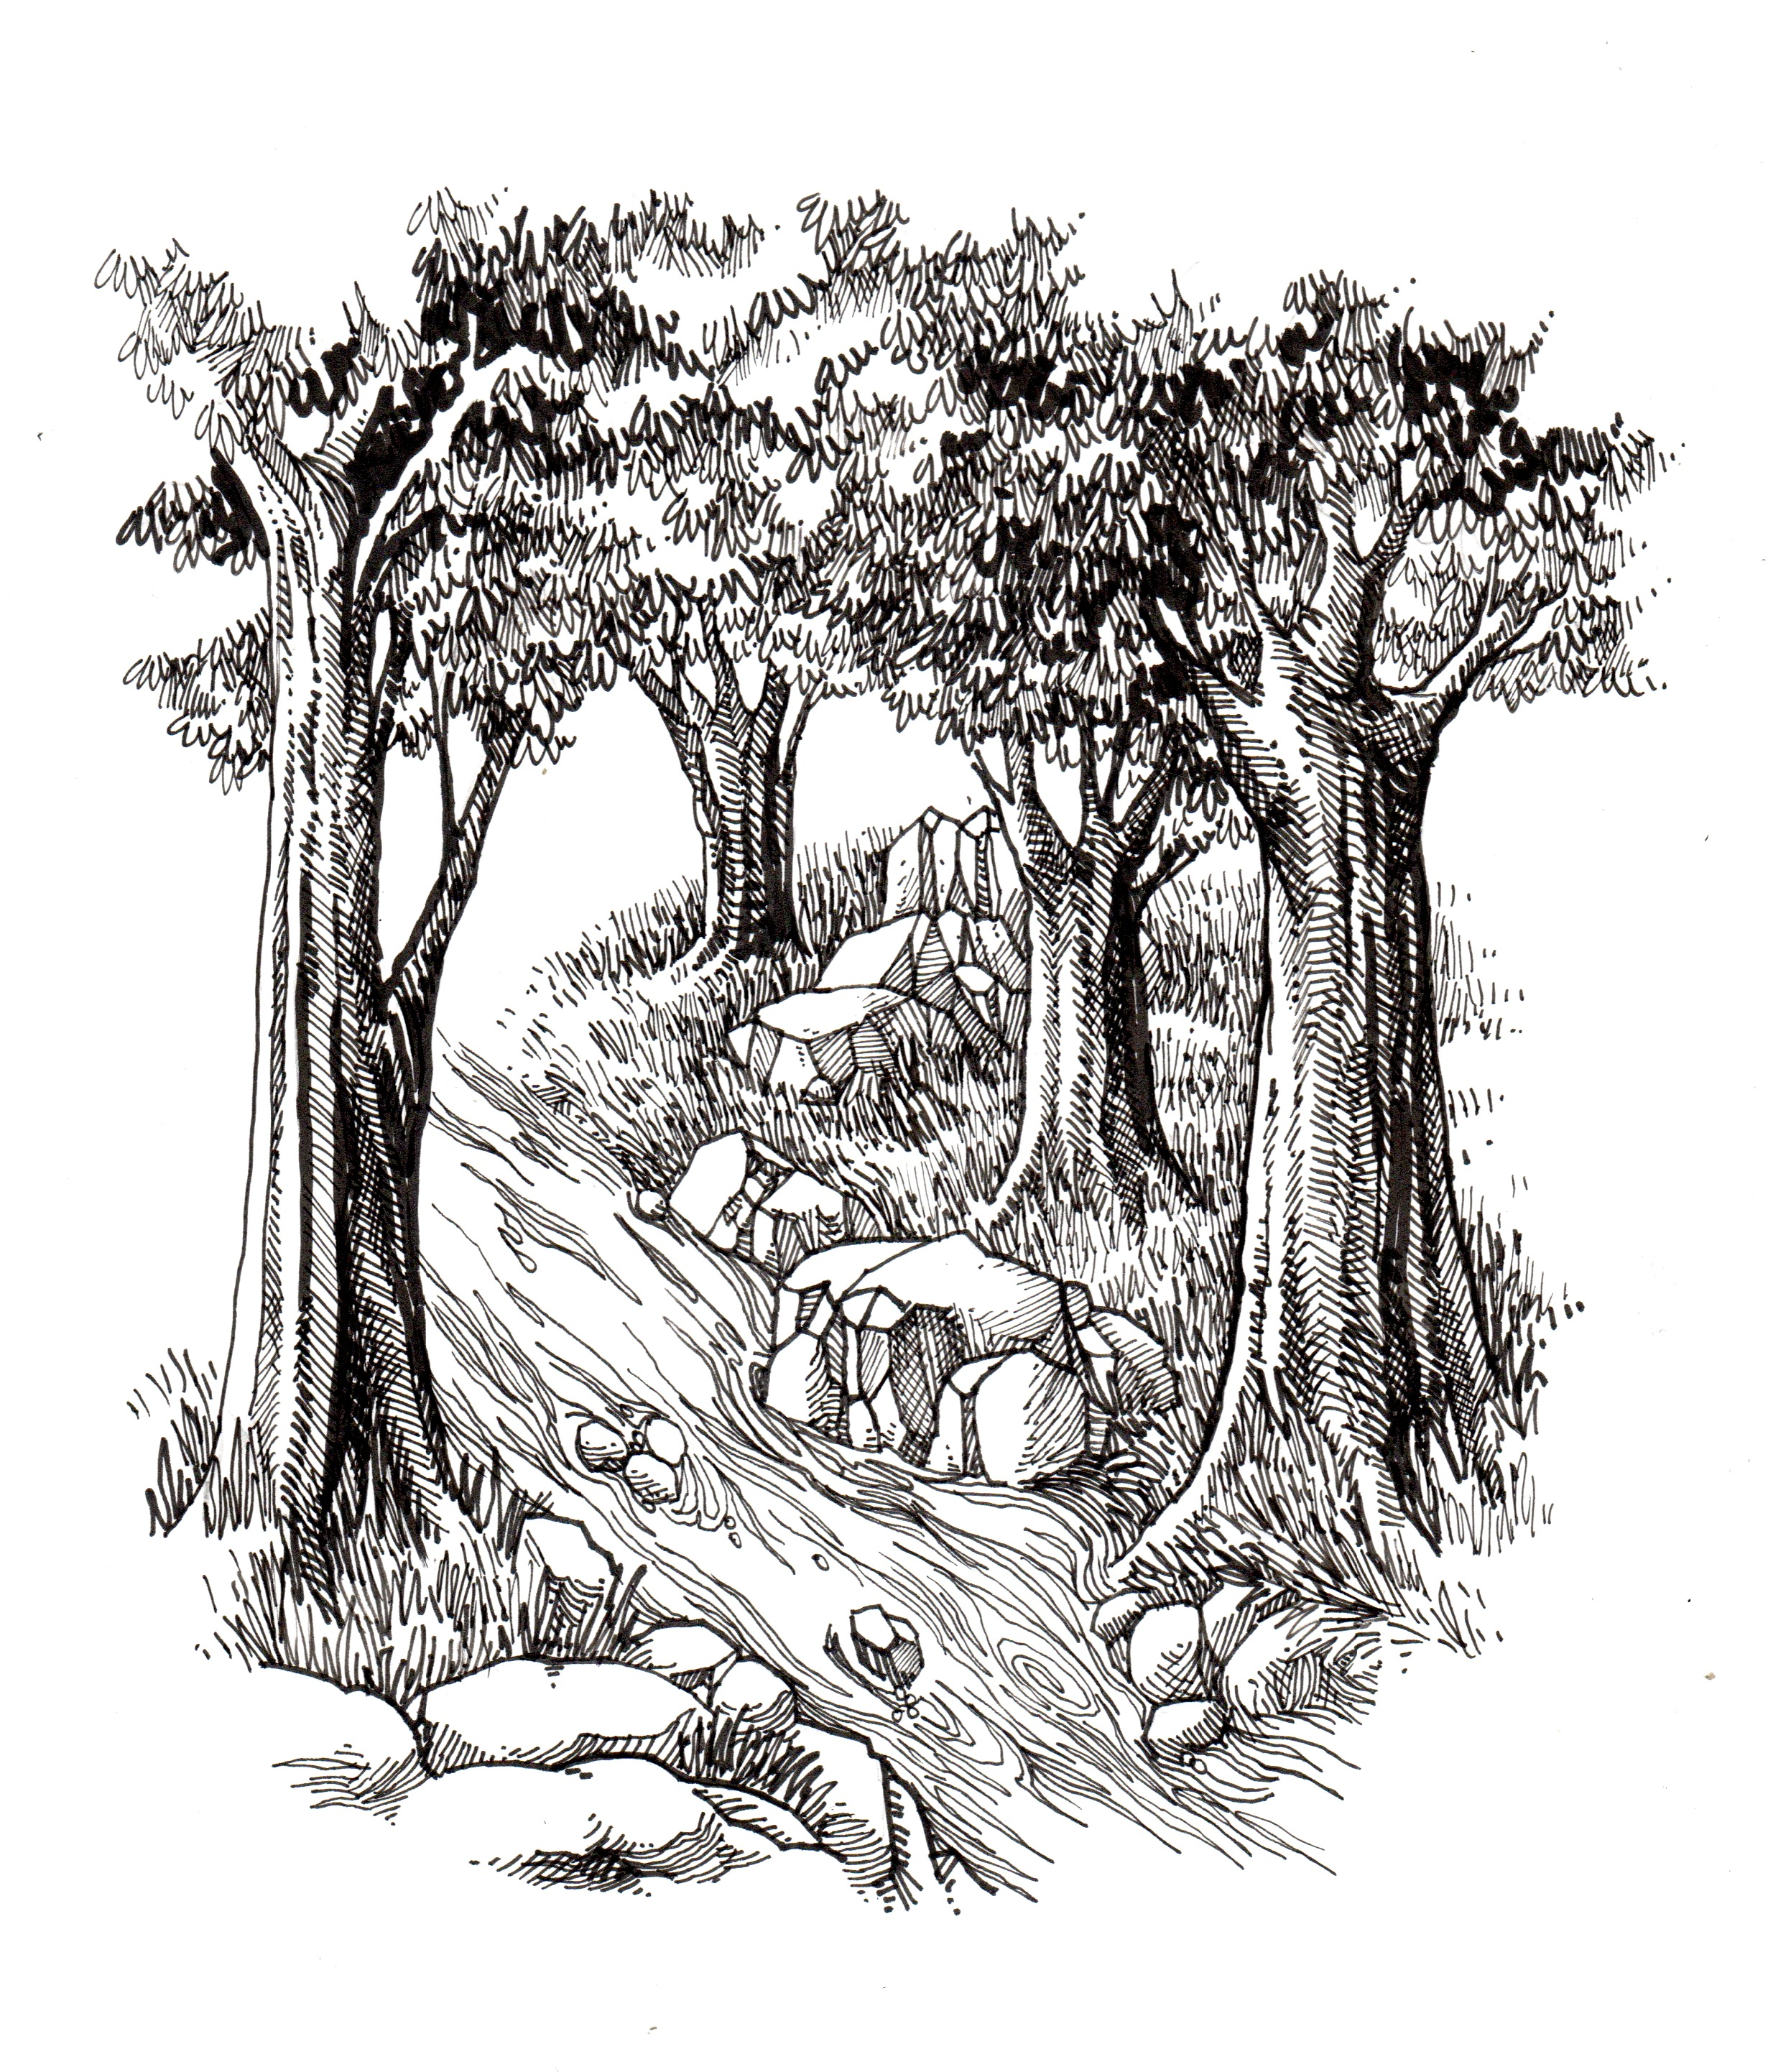
\includegraphics[width=0.6\linewidth,height=\textheight,keepaspectratio]{images/introduction.jpeg}

}

\caption{Jordan River}

\end{figure}%

\epigraph{
Institutions of higher learning in fact have a long history of association with the garden, be it the parks and groves of the famous Greek schools, the Roman villa, the bowers of Sainte-Geneviève in medieval Paris, the Italian garden academies of the Renaissance, the British "college garden," or the idyll of the traditional American campus. The question that interests us here is whether there is more to this association than just a matter of setting. }
{\parbox{.75\textwidth}{\raggedleft---Robert Pogue Harrison, \textit{Gardens: An Essay on the Human Condition}}}

A university's natural environment, modified by human intervention,
provides more than a setting for higher education. The physical campus
becomes part and parcel of institutional image, identity, and integrity.
``The singular magic of a place is evident from what happens there, from
what befalls oneself or others when in its vicinity,'' ecological
philosopher David Abram has written. ``To tell of such events is
implicitly to tell of the particular power of that site, and indeed to
participate in its expressive potency.''\footnote{\citeproc{ref-abram1996a}{David
  Abram, \emph{The Spell of the Sensuous: Perception and Language in a
  More-Than-Human World} (New York: Vintage, 1996), 182}.} By touching
the place with hands and eyes, by walking through it and observing the
interacting patterns of natural landscape and built environment, by
listening to and reading stories about the lore of the place and its
denizens, one might activate an ancient and ineffable sensibility. This
book explores how history and landscape and place-making contribute to
Indiana University (IU)'s institutional identity.

\section*{Voices along the Way}\label{voices-along-the-way}
\addcontentsline{toc}{section}{Voices along the Way}

\markright{Voices along the Way}

Between 1890 and 1977, a handful of books dealing with the narrative
history of IU were published. The authors were faculty men, nearly all
of whom were retired. These books' content reflected a loose consensus
on the dominant themes found in the institution's history. Among them
were the value of public education, the worth of individual students,
curricular changes responding to social needs, the academic community at
the juncture of intellectual ideals and practical living, the symbiosis
between students and teachers, and the animating ideal of research as
the basis for knowledge.\footnote{\citeproc{ref-wylie1890a}{Theophilus
  A. Wylie, \emph{Indiana University, Its History from 1820, When
  Founded, to 1890, with Biographical Sketches of Its Presidents,
  Professor and Graduates, and a List of Its Students from 1820 to 1887}
  (Indianapolis: Wm. B. Burford, 1890)};
  \citeproc{ref-harding1904a}{Samuel Bannister Harding, ed.,
  \emph{Indiana University, 1820--1904} (Bloomington: Indiana
  University, 1904)}; \citeproc{ref-woodburn1940a}{James A. Woodburn,
  \emph{History of Indiana University: Volume {I}, 1820--1902}
  (Bloomington: Indiana University, 1940)};
  \citeproc{ref-myers1952a}{Burton Dorr Myers, \emph{History of Indiana
  University: Volume {II}, 1902--1937, {The} Bryan Administration}, ed.
  Burton D. Myers and Ivy L. Chamness (Bloomington: Indiana University,
  1952)}; \citeproc{ref-clark1970a}{Thomas D. Clark, \emph{Indiana
  University: Midwestern Pioneer}, 4 vols. (Bloomington: Indiana
  University Press, 1970/1977)}.}

But general narratives are but one form of university history at IU.
Casting a wider net, one finds program, department, school, or campus
histories; studies of student life; biographical directories of
administrative officers and trustees; autobiographies, memoirs, and
biographies; and various thematic and topical works. They defy easy
summary since they vary widely in tone, approach, and length. Their
authorial demography, perhaps not surprisingly, is more diverse in
gender, ethnicity, and age---although the vast majority have either
worked or studied at IU.\footnote{See
  \href{https://guides.libraries.indiana.edu/iuarchives_howto}{``How To
  Conduct Research at the IU Libraries University Archives''}.}

In 2020, Indiana University commemorated its 200\textsuperscript{th}
anniversary with a broad and inclusive public history
program.\footnote{\citeproc{ref-iu2020a}{Office of the Bicentennial,
  {``Indiana University Bicentennial Final Report''} (Bloomington:
  Indiana University, 2020),
  \url{https://wayback.archive-it.org/219/20240413230003/https://200.iu.edu/doc/IU-bicentennial-final.pdf}}.}
One of its goals was to engage critically with past institutional
narratives; to reexamine their assumptions, sources, and methods; and to
write new, empirically based historical accounts that take a more
inclusive and equitable approach that does not privilege one set of
historical actors over another. In this way, more voices could be heard
as well as new perspectives explored, especially ones that are
underrepresented in existing histories.

This book focuses attention on record-keepers (archivists, historians,
editors, faculty, and staff) who preserve, make accessible, and
interpret written documentation about university programs, events, and
people. In addition, because the campus is the physical embodiment of
the institution, and it too has a history, physical plant staff
(planners, architects, landscapers, gardeners, and groundskeepers)
receive consideration as well.

\section*{Emplacing the University}\label{emplacing-the-university}
\addcontentsline{toc}{section}{Emplacing the University}

\markright{Emplacing the University}

Persistent lacunae in IU's historiography are the role of place and the
process of place-making as key components of institutional image and
historical identity. This is ironic because members of the university
community have been touting the beauty of the flagship campus in
Bloomington since the late 1800s. In more recent times, outside experts
comparing campus design and facilities implementation across the nation
judge IU to be in the top rank regularly. How and why did the university
develop ``America's legacy campus,'' as a recent book title phrased it,
and what were the institutional consequences of possessing a vivid sense
of place?\footnote{See Thomas A. Gaines,
  \citeproc{ref-gaines1991a}{\emph{The Campus as a Work of Art}
  (Westport, CT: Praeger, 1991)}, for comparative campus analysis; and
  J. Terry Clapacs, \citeproc{ref-clapacs2017a}{\emph{Indiana University
  Bloomington: America's Legacy Campus} (Bloomington: Indiana University
  Press, 2017)}, for his use of ``America's legacy campus.''}

Focusing on place might open new conceptual horizons. It can be argued
that the campus itself has a measure of historical agency, albeit a
nonhuman one. Its assemblage of natural elements and processes provides
a unique environment of opportunities and constraints. From this
perspective, the campus serves as the place where the university is
enacted and the academic community is, both literally and
metaphorically, grounded. It follows that the design and operations of
the physical plant are historically important, and so the work of campus
planners, architects of structures and landscapes, and caretakers and
gardeners assume a renewed significance. Such individuals express their
intentions in the media of stone, brick, and wood used for buildings and
other campus facilities or in a vegetal palette of trees, shrubs,
grasses, and flowers. The choices made by architects of buildings and
landscapes are rooted in the rich traditions and disciplines of design,
captured at a specific moment, as they shape the physical plant. The
resulting visual image and tactile feel of the campus became part of the
university's historical identity that cannot be completely conveyed in
words.

Sense of place is built on historical and experiential knowledge of a
particular locality. Relevant past work includes IU political scientist
Lynton K. Caldwell's brief foreword to the encyclopedic survey \emph{The
Natural Heritage of Indiana}, in which he distinguishes ``natural
features are what they are and where they are without regard to human
presence'' and places ``defined by human perception.'' Thus, ``the
qualities and characteristics defining a place express not only its
biophysical attributes, but also its aesthetic value and historic
significance.''\footnote{\citeproc{ref-caldwell1997a}{Lynton Keith
  Caldwell, {``Foreword: A Sense of Place,''} in \emph{The Natural
  Heritage of Indiana}, ed. Marion C. Jackson (Bloomington: Indiana
  University Press, 1997), xvi}.} Near the start of the twenty-first
century, three IU professors in the humanities and arts---Will Counts,
James Madison, and Scott Sanders---composed a portrait of Bloomington in
words and photographs, attempting to capture the special qualities of
the community. Explaining their approach and motivation, the preface
states, ``Good places are shaped by the gifts of nature and by the labor
and love of many people over generations. The city of Bloomington,
tucked away in the forested hills of southern Indiana, is one such
place. Three of us who have worked here, played here, reared children
here, and set our roots right down to the limestone bedrock made this
book to chronicle and celebrate our home town.''\footnote{\citeproc{ref-counts2002a}{Will
  Counts, James H. Madison, and Scott Russell Sanders, \emph{Bloomington
  Past and Present} (Bloomington: Indiana University Press, 2002), x}.}
In my own previous historical work, I have employed the concept of
\emph{genius loci} to shed light on the activities of IU administrator
Herman Wells at Indiana University.\footnote{\citeproc{ref-capshew2011a}{James
  H. Capshew, {``Indiana University as the {`Mother of College
  Presidents'}: Herman {B} Wells as Inheritor, Exemplar, and Agent''}
  (Bloomington: IU Institute for Advanced Study, 2011),
  \url{https://hdl.handle.net/2022/14123}};
  \citeproc{ref-capshew2012a}{James H. Capshew, \emph{Herman {B} Wells:
  The Promise of the American University} (Bloomington; Indianapolis:
  Indiana University Press; Indiana Historical Society Press, 2012)}.}

\section*{Plan of the Book}\label{plan-of-the-book}
\addcontentsline{toc}{section}{Plan of the Book}

\markright{Plan of the Book}

This volume is divided into three parts. The
\hyperref[sec-partone]{first} deals with origins and beginnings.
Chapter~\ref{sec-one} locates the nascent institution in a new town in a
new state, painting with a broad brush some salient features of the
frontier environment and culture. Chapter~\ref{sec-two} recounts the
story of the first teacher, the Reverend Baynard Rush Hall, and his
career. Because much of what we know today about the institution's early
history came from his 1843 book \emph{The New Purchase}, he also
qualifies as the first historian. Chapter~\ref{sec-three} deals with how
a distinct genre of historical writing about Indiana University arose in
the 1890s in response to significant changes in the university. An 1883
campus fire led to a decision to move the campus to a more promising
locale and an 1884 presidential scandal caused a change in leadership
that catalyzed serious historical reflection for the first time. With
deep connections to IU and representing different generations, three
individuals---Theophilus Wylie (1810--95), David Banta (1833--96), and
James Woodburn (1856--1943)---composed narratives of institutional
progress circa 1890 as a response to the move to Dunn's Woods and the
fresh leadership of David Starr Jordan. They anchored the university in
the collective memory of the community and gave voice to institutional
aspirations for the future. The subsequent career of institutional
history is sketched, with critical commentary.

\hyperref[sec-parttwo]{Part Two} analyzes the design history of the
flagship campus at Dunn's Woods. The narrative reveals a remarkable
consensus about conserving the native woodland character of the
landscape at the beginning and then enduring persistence in extending
that vision as the campus grew one hundredfold, from twenty to 2,000
acres. The result of that extraordinary fidelity to local conditions was
a cultural landscape of acknowledged beauty and integrity.
Chapter~\ref{sec-four} opens with the university moving to a new campus
in 1885, having outgrown the original Seminary Square location that had
served as the site of instruction for sixty years. A fateful decision in
the ordinary course of building placement nudged the university
community toward a variation of the medieval Gothic quadrangle as the
campus design evolved organically. The remnant forest was preserved as
new buildings, made of local limestone, were constructed to frame Dunn's
Woods in a giant quadrangle. By 1915, two out of four sides of the frame
had been completed and a start made on the remaining two sides.
Chapter~\ref{sec-five} explores the period between 1915 and 1945, when
additional lands were purchased and the campus moved beyond the great
quadrangle that married the gray stone buildings and the green woods.
Further development occurred on Third, Seventh, and Tenth Streets, and
Jordan Avenue (now Eagleson Avenue) was built to provide a boundary on
the east. The woodland theme was carried through by the preservation or
renovation of green spaces as the campus acquired specialized facilities
(e.g., athletic stadium), accommodated the proliferation of professional
schools (e.g., music, education, business), and started housing students
on campus. Attentive members of the academic community noted the
delights that the Indiana campus held. The chapter ends with the
disruptions caused by the economic woes of the 1930s and the
mobilization for the Second World War. Chapter~\ref{sec-six} covers 1945
to 1980, a time that saw an exponential increase in the campus
footprint, to about 2,000 acres, designed to accommodate tremendous
growth in student enrollments, academic programs, and athletic
facilities. With this increase in scale, the pace of campus development
quickened as well, and the campus grew into its present configuration,
roughly divided into zones for academic structures, residential life,
and athletic and sports facilities. Chapter~\ref{sec-seven} analyzes the
decades 1980 to 2020, a period characterized by increased attention to
historic preservation and focused infill. Renovation and rehabilitation
of existing structures began in earnest in the mid-1980s, starting with
the repurposing of the old stadium into an arboretum, followed later by
the restoration of the buildings comprising the original Old Crescent
surrounding Dunn's Woods. At times, the modern physical plant stretched,
but did not break, the century-old conservationist ethos that has been
transformed in the twenty-first century into a search for environmental
sustainability.

\hyperref[sec-partthree]{Part 3} offers another route into place-making,
focusing on narratives and stories that emplace Indiana University into
historical contexts. Sometimes references about literal places are
absent but implied. The point is that our perceptions and understandings
of Indiana University as an institution are shaped and conditioned by
historical narrative. Using a biographical approach,
Chapter~\ref{sec-eight} analyzes the little-known career of Ivy L.
Chamness (1881--1975), the first (and only) person to hold the title of
editor of university publications (1917--52). The chapter focuses on her
work on behalf of university history, as editor of the \emph{Indiana
University Alumni Quarterly}, as developmental editor for both volumes
of the official \emph{History of Indiana University}, and as a
contributing historical writer. Because she was a woman in a patriarchal
society, Chamness's significant historical contributions were
undervalued during her career and subsequently overlooked. The evidence
demonstrates that she was the linchpin that kept the practice of IU
history going through the mid-twentieth century. Chapter~\ref{sec-nine}
explores the practice of honoring deceased faculty members by memorial
resolutions written by faculty colleagues. Highlighting the human
quality of the institution, faculty careers of teaching, research, and
service are the warp threads of the tapestry that is the university
while the students are the weft yarns. The contributions of two key
faculty members---chemistry professor Harry Day (1906--2007) and English
professor Donald J. Gray (b. 1927)---are examined in their roles as
university necrologists. Chapter~\ref{sec-ten} reexamines the role of IU
administrator Herman Wells (1902--2000) in the preservation of the 1835
house built by Andrew Wylie, the first president. Beginning with his
first encounters in the 1930s as a young faculty member, Wells developed
a lifetime commitment to the historic house, the most significant
artifact remaining from the early history of Indiana University. In his
lengthy career as president (1937--62) and university chancellor
(1962--2000), he was responsible for the university's initial
acquisition of the house in the 1940s and was involved with decisions
for architectural restoration in the 1960s and its gradual emergence as
an operating museum in the 1980s. The history of that relationship is
explored at length, echoing themes of materiality and identity.

A brief \hyperref[sec-coda]{coda}, occasioned by the 2020 global
pandemic, allows reflection on the meaning of the term \emph{watershed},
taken literally and figuratively. Used to periodize the 200-year history
of Indiana University, it can connect history, landscape, and sense of
place in constructive ways.

This book is built around the notion that writing institutional history
should be a multivocal, iterative, and cumulative process. Multivocal in
the sense that the subjects of analysis are individuals from all strata
and positions in the university and that a variety of sources is used.
History is never finally done, once and for all. Fundamentally an
iterative process, there can only be the latest revision to contend with
prior interpretations. New sources and different angles of vision can
occasion revisions of old stories and help one comprehend how
interpretation changes over time. Institutional history is also
cumulative: each work has the potential to enhance our current
understanding. This historical accumulation creates practical problems
for attempts to comprehensively portray an institution over a long span
of time, however. It can be done, but there are reasons that the last
comprehensive narrative of Indiana University was written fifty years
ago in a tome of 1,500 pages in three volumes.\footnote{\citeproc{ref-clark1970a}{Clark,
  \emph{Indiana University}, 1970/1977}.}

I hope these chapters remind us that a shared institutional history can
be an abundant tapestry that weaves together the stories of students,
faculty, staff, alumni, donors, citizens, and visitors even though their
individual experiences might vary widely and differ profoundly. The
university's campus can be seen as a palimpsest inscribed with a record
of interventions and mediations---great and small, temporary and
permanent---of both the human and the nonhuman environment. Everyone can
learn to observe and think of the past within the present, to discern
enduring design patterns within the campus landscape as well as the
human intentionality within its structures of values and goals. There
are benefits to be gained and insights to be gleaned in understanding
the past writers of our present history, whether that history is written
in ink, chiseled limestone, or the ground beneath our feet.\footnote{\citeproc{ref-sandweiss2024a}{Eric
  Sandweiss, {``Personal Communication to the Author,''} June 7, 2024}.}

\bookmarksetup{startatroot}

\chapter*{Part One: Provenance}\label{sec-partone}
\addcontentsline{toc}{chapter}{Part One: Provenance}

\markboth{Part One: Provenance}{Part One: Provenance}

\epigraph{
Each age writes the history of the past anew with reference to the conditions uppermost in its own time.} 
{---Frederick Jackson Turner, \textit{The Significance of History}}

\begin{figure}[H]

{\centering \pandocbounded{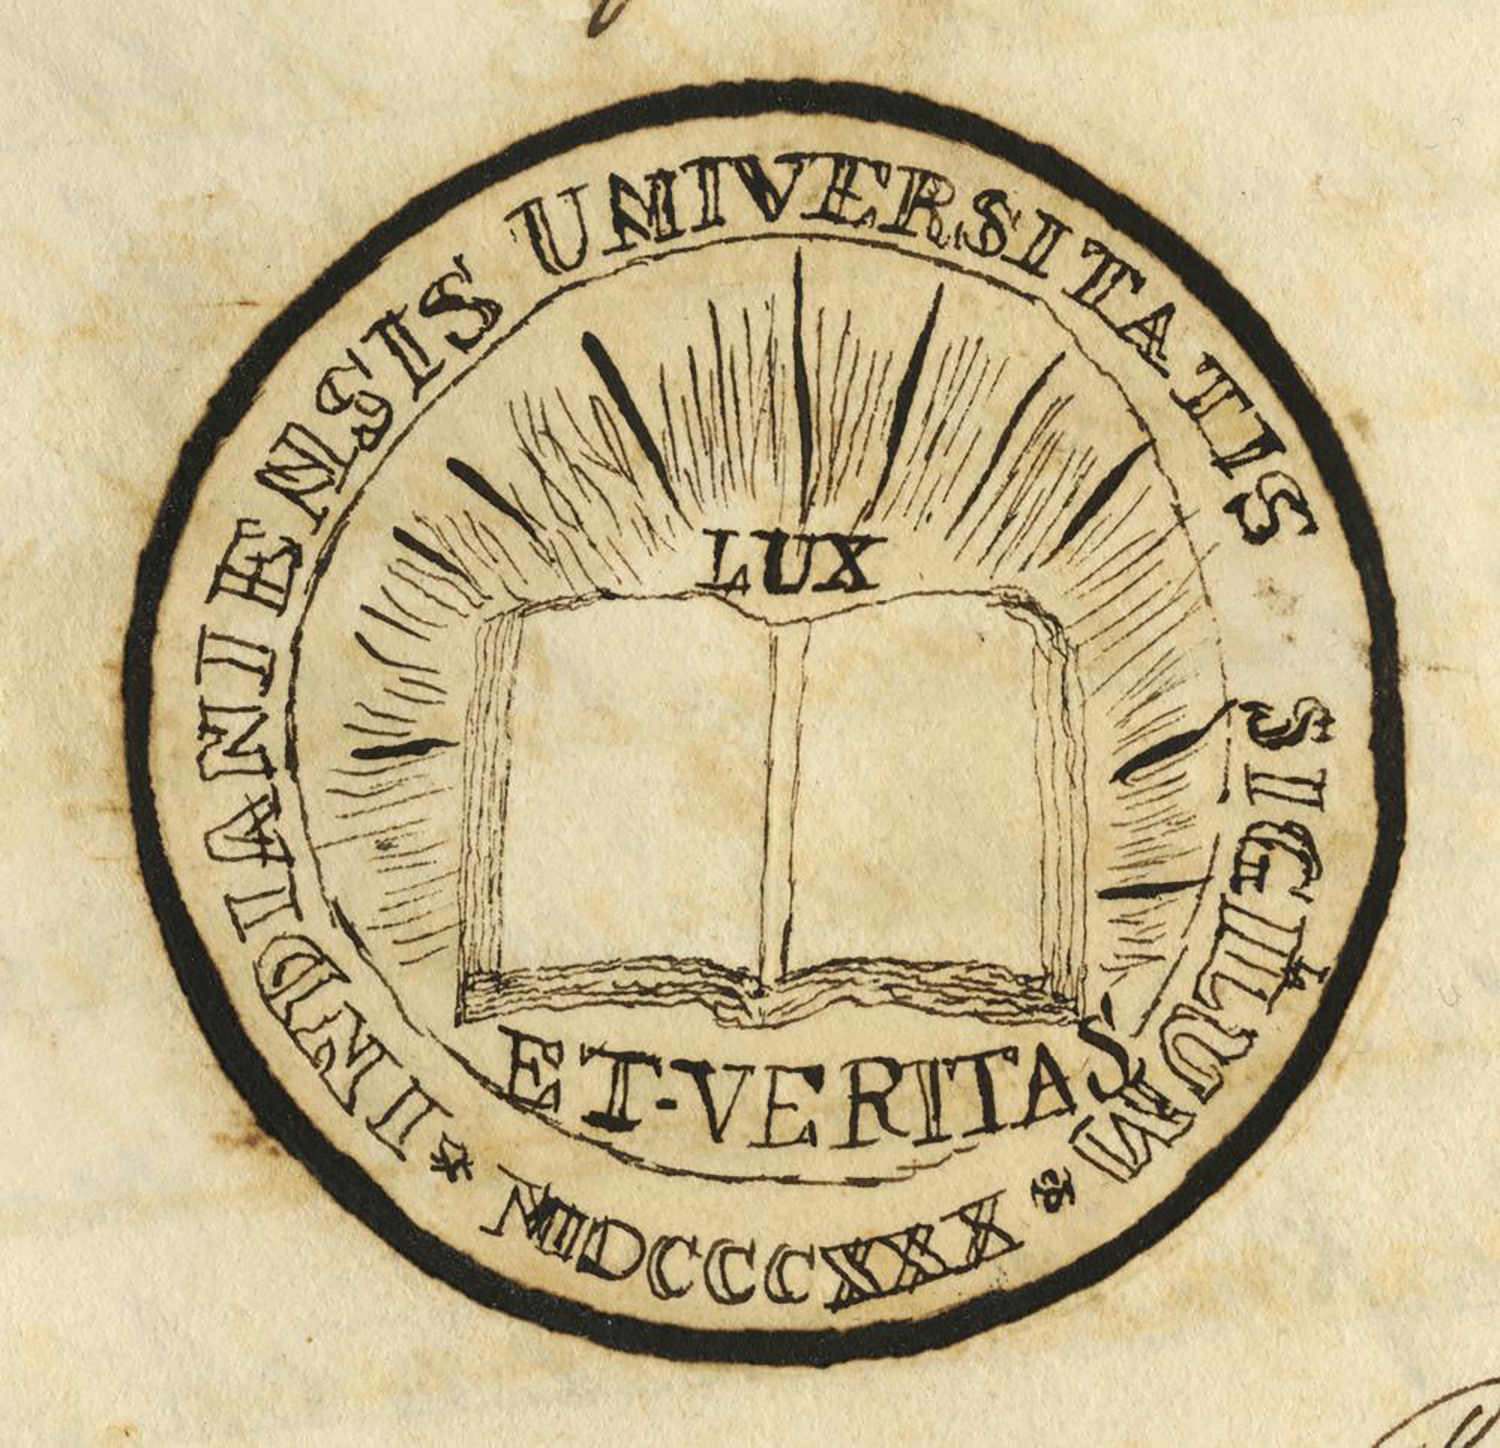
\includegraphics[keepaspectratio]{images/uniseal.jpg}}

}

\caption[First Image of Indiana University Seal]{First image of the
Indiana University seal. Hand-drawn in the manuscript minutes of the
Indiana University Board of Trustees, July 21, 1841. \textbf{© Indiana
University. Image from the
\href{https://libraries.indiana.edu/university-archives}{IU Archives}.}}

\end{figure}%

\bookmarksetup{startatroot}

\chapter{First the Forests}\label{sec-one}

\begin{figure}[H]

{\centering 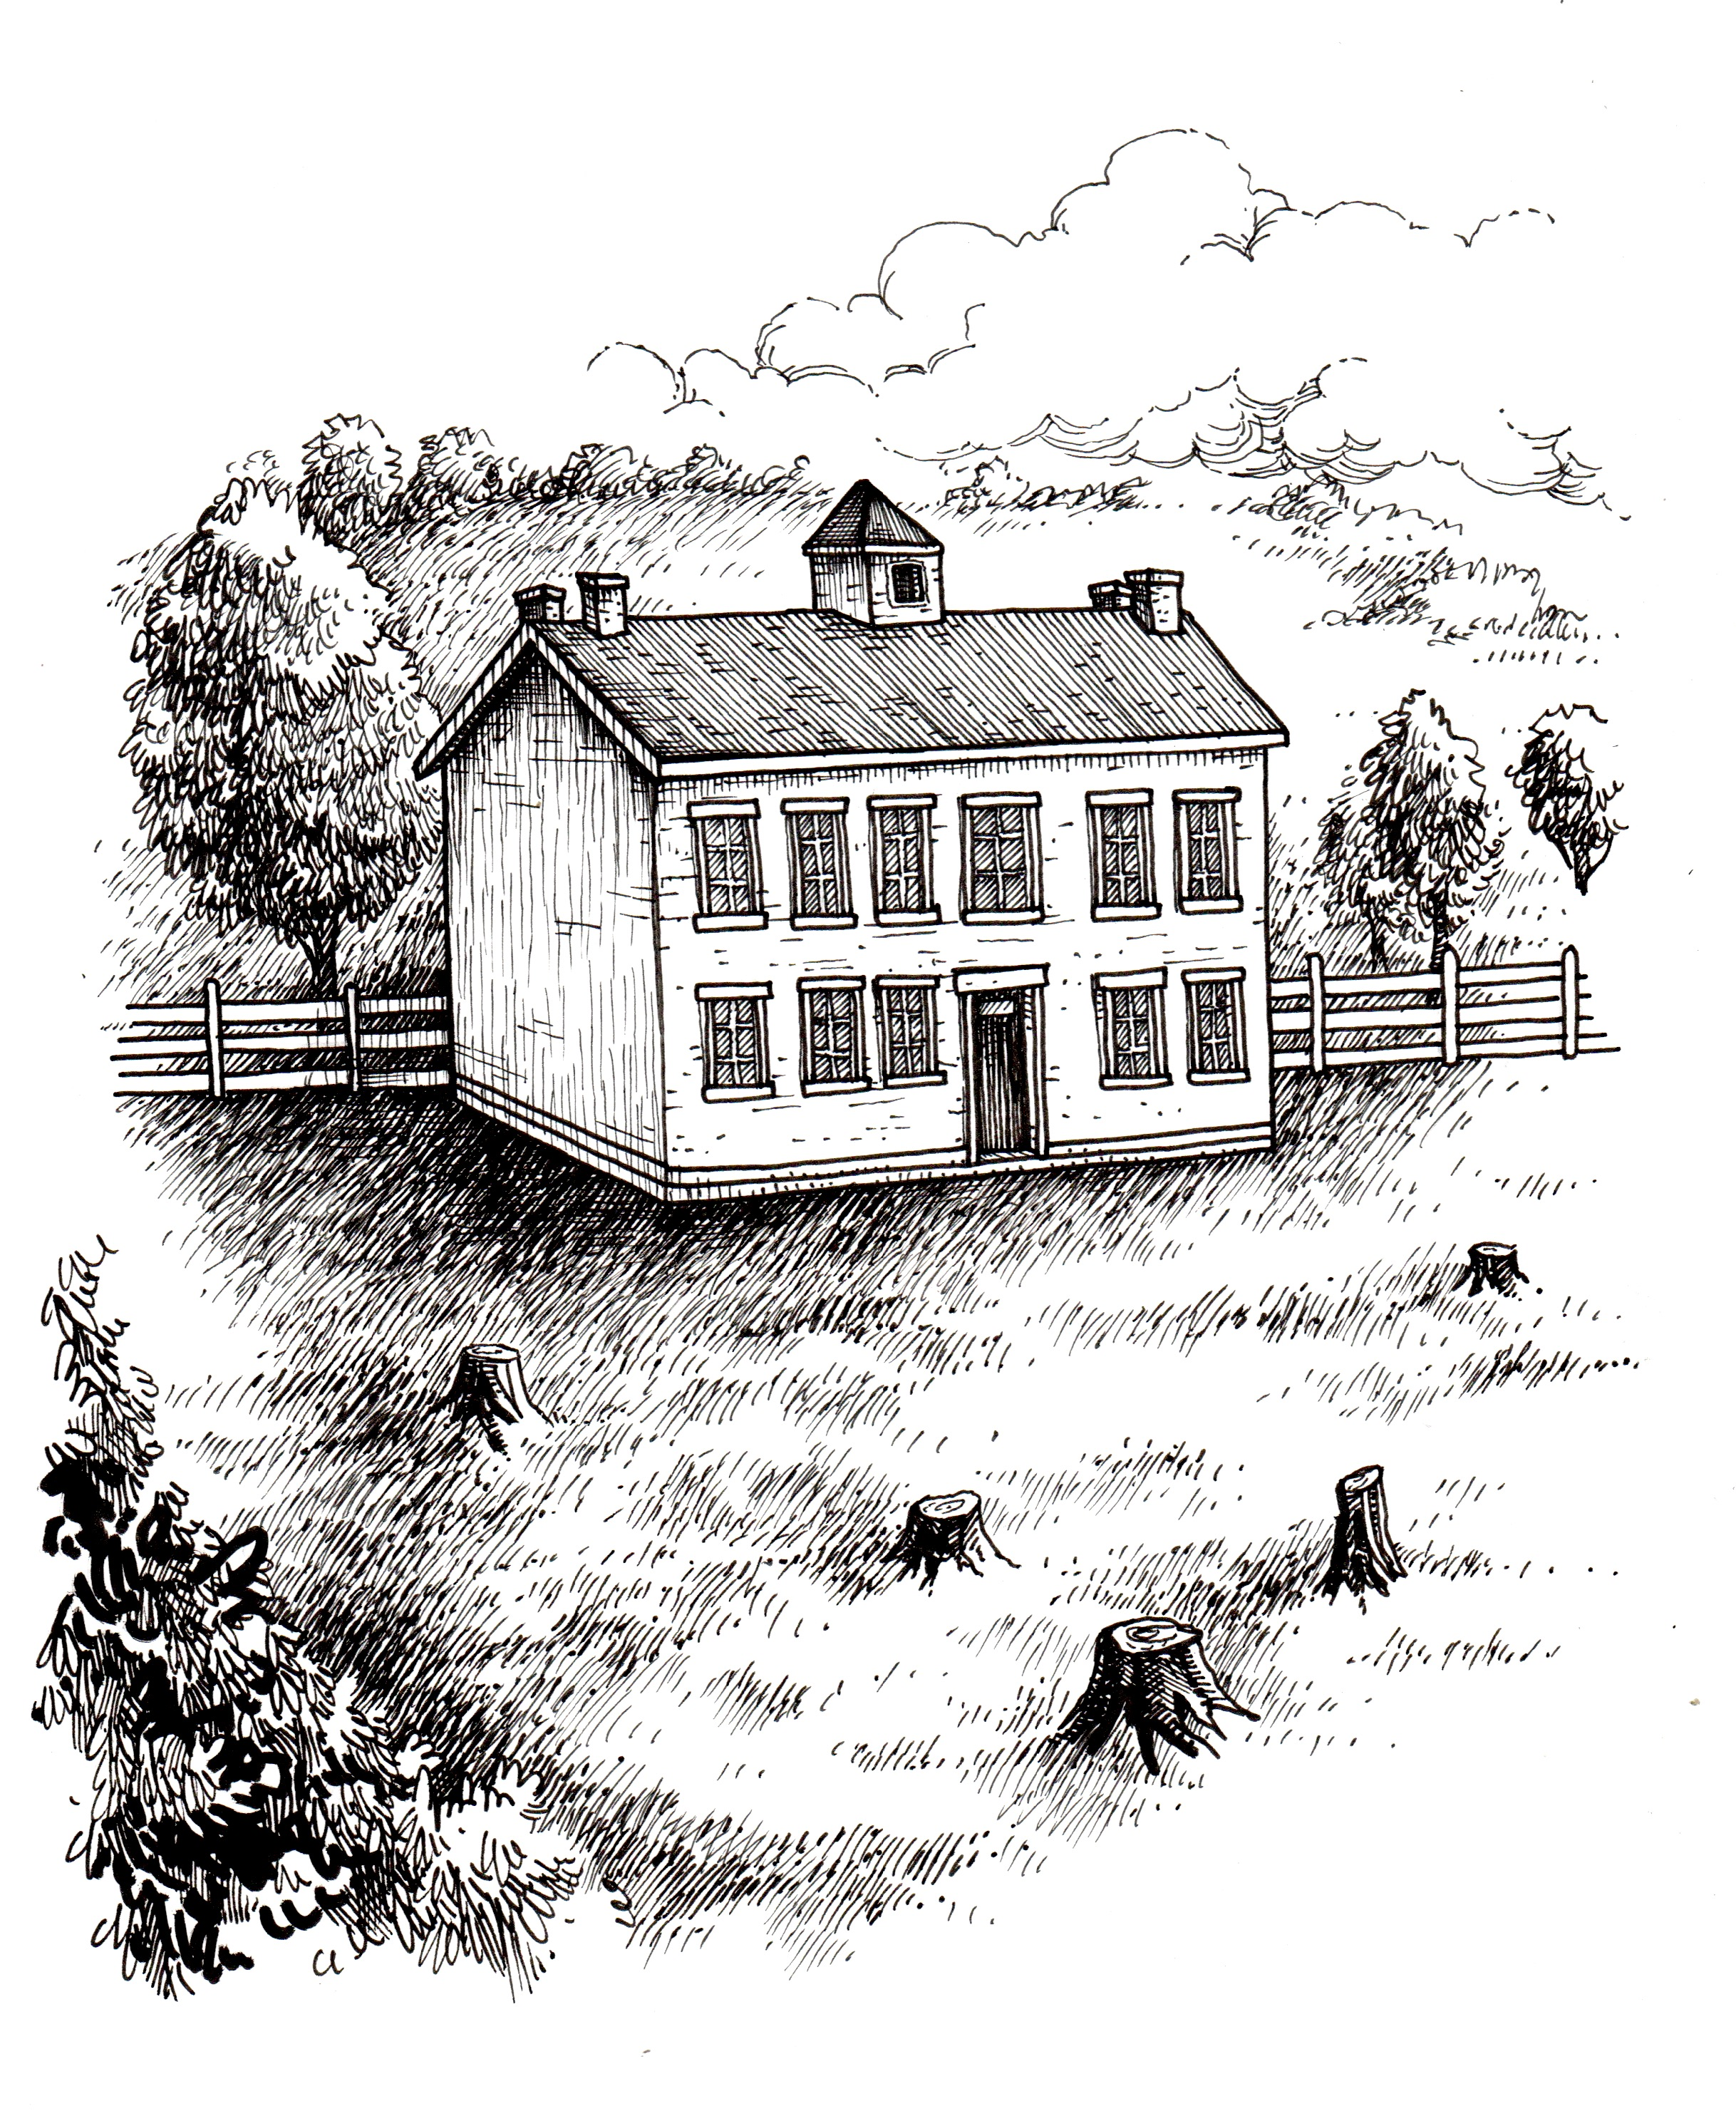
\includegraphics[width=0.6\linewidth,height=\textheight,keepaspectratio]{images/miu1.jpeg}

}

\caption{Seminary Building}

\end{figure}%

\epigraph{
This was the order of human institutions: first the forests, after that the huts, then the villages, next the cities, and finally the academies.} 
{---Giambattista Vico, \textit{The New Science}}

In the beginning, there was the land, covered by a vast deciduous
forest. Far from empty, it was full of vegetative life and animals of
every size, including humans. Indigenous people lived within this
natural abundance---hunting, fishing, and gathering plants for food,
shelter, and medicine.

After the Revolutionary War created the United States of America, the
Northwest Territory (spanning six eventual states: Ohio, Indiana,
Illinois, Michigan, Wisconsin, and Minnesota) was developed in the
late-eighteenth century. European migrants moved in to occupy the
homelands of native communities. Treaty after treaty gave a legal gloss
to systematic genocidal terror as Indigenous peoples were forcibly
removed and property rights were retained by the federal government.
Ironically, their absence defined the beginning of ``the land of the
Indians''---Indiana---and left deep scars from a historical trauma yet
to be reconciled.

As the white population increased to 60,000 (the threshold to petition
for statehood), the state of Indiana was carved out of the Indiana
Territory in 1816.\footnote{\citeproc{ref-madison2014a}{James H.
  Madison, \emph{Hoosiers: A New History of Indiana} (Bloomington:
  Indiana University Press; Indiana Historical Society Press, 2014),
  49}.} The Seventh US Congress granted a township of land (six miles by
six miles square, or 23,040 acres) to support a seminary of
learning.\footnote{See \citeproc{ref-cep2011a}{Center on Education
  Policy, {``Public Schools and the Original Federal Land Grant Program:
  A Background Paper from the Center on Education Policy''} (Washington,
  2011-04), \url{https://eric.ed.gov/?id=ED518388}}.} In 1818, that
location became Perry Township in the new county of Monroe. The recently
concluded Treaty of St.~Mary's ceded Native American lands comprising
the central third of the state and was known as the New Purchase. In the
southern portion of the New Purchase, Monroe County marked the northern
extent of white settlement in the new state.

On January 20, 1820, the Indiana General Assembly passed a bill to
establish a state seminary of learning and designated a board of
trustees to oversee its operation. The board, headed by physician David
H. Maxwell from the new village of Bloomington (population 300), decided
to locate the new seminary in Perry Township on seminary lands, although
they could have located it anywhere in the state. They selected a
ten-acre site with a spring a quarter mile south of the county
courthouse square for the campus of the Indiana State Seminary. Other
seminary township lands were sold to provide a meager endowment for the
school.

The site was cleared of trees and other vegetation, marking an opening
in the wild forest. The trustees hired contractors to build a classroom
building and a professor's house. The next order of business was to find
an instructor who could teach Greek and Latin, the foundation of the
classical curriculum derived from medieval European roots. As it
happened, a Presbyterian minister, Baynard Rush Hall, had moved to
Monroe County recently, and, as he later boasted, he was ``the very
first man since the creation of the world that read Greek in the New
Purchase!''\footnote{\citeproc{ref-hall1916a}{Baynard Rush (Robert
  Carlton, pseud.) Hall, \emph{The New Purchase, or, Seven and a Half
  Years in the Far West}, ed. J. A. Woodburn (1843; repr., Princeton
  University Press, 1916), 158}.} Finally, preparations were complete,
and the seminary opened in April 1825, with a dozen young men comprising
the student body and Hall as the sole faculty member.

\section{Pioneer Bloomington}\label{pioneer-bloomington}

Getting to Bloomington required overland travel, typically by horseback,
stagecoach, or walking. In the frontier village, log cabins abounded,
and the rudimentary dirt roads were full of stumps and turned into muddy
messes when it rained. Heating and cooking were managed by stove or
fireplace, and the provision of firewood was a constant concern.
Residents obtained their food by growing vegetables in home gardens and
possessing flocks of chickens, which ranged freely. Hunting wild game as
well as slaughtering pigs and cows supplemented diets with meat.

As the population slowly grew, the amount of land cleared for the
construction of houses and crops increased, and the village became more
economically diversified and socially stratified. In 1828, the general
assembly raised the seminary to the status of a college---Indiana
College---and the trustees offered its presidency to Andrew Wylie, a
Presbyterian minister who had been a college president in western
Pennsylvania. Wylie took up his duties in 1829, joining a faculty of two
and a student body of nearly forty. Plans were drawn up for a new
college building to provide additional classrooms, a library, and a
chemical laboratory. The first commencement, in 1830, celebrated the
achievements of four students who had completed the college course.

In 1833, Cornelius Pering, along with his family, arrived in Bloomington
to teach in the nascent Monroe County Female Seminary. An Englishman, he
immigrated to the United States the year before. His observations of
Bloomington were keen, and he described the small settlement in words
and drawings. He noted the ubiquity of tree stumps, including on the
rustic unfinished campus: ``You will observe that the land has been
recently cleared, and that the stumps of the trees are not yet entirely
rotten. Trees are always cut down with the axe a foot or two from the
ground and the stumps left to rot, which they do in eight or ten
years.''\footnote{\citeproc{ref-pering1933a}{Cornelius Pering, {``The
  Pering Letters of 1833,''} \emph{Indiana University Alumni Quarterly},
  no. 20 (1933): 420}.}

The first professor, Baynard Hall, who had left in 1832, lamented the
wholesale clearing of the land for the campus. Looking back in 1843, he
wrote, ``That a most sumptuous area had already been marred by the
ignorance and cupidity of planners and builders; and among other
irremediable evils, not a grove of forest trees had been left standing
on the campus.''\footnote{\citeproc{ref-hall1916a}{Hall, \emph{The New
  Purchase, or, Seven and a Half Years in the Far West}, 1916, 71}.} The
great hardwood forests of Indiana were only beginning to be exploited
for economic gains at that time, and little attention was paid to other
values, including their aesthetic beauty.

\section{Original Campus}\label{original-campus}

In 1835, President Wylie and his wife, Margaret, moved their large
family into an imposing two-story brick house located near the college
on a twenty-acre farmstead. One of the finest houses in the county, it
was a marker of their social status. Meanwhile, the new College Building
experienced prolonged delays in construction and was finally opened in
1836. The three-story brick structure was set on a foundation of
limestone. Its design was inspired by ``a picture of a New England
cotton factory {[}found{]} on a bolt of muslin in one of the stores of
Bloomington'' seen by one of the trustees.\footnote{\citeproc{ref-cravens1922a}{John
  W. Cravens, {``Buildings on the Old and New Campuses of Indiana
  University: II: Six of the Buildings on the Old Campus,''}
  \emph{Indiana University Alumni Quarterly} 9, no. 2 (1922): 158}.} It
housed the chapel, ample recitation rooms, and rooms for the Athenian
and Philomathean student literary societies.

In 1838, with the campus as a going concern in the small town of 1,500,
the college was legislatively transformed yet again, into Indiana
University, with plans for schools of medicine and law to be
established.\footnote{See \citeproc{ref-woodburn1940a}{Woodburn,
  \emph{History of Indiana University}, 1940, 118}.} That year, the
Boarding-House was erected, incorporating the professor's house in its
structure. It provided accommodation for thirty to forty students, and
residents could grow their own vegetables on the campus.\footnote{\citeproc{ref-cravens1922a}{Cravens,
  {``Buildings on the Old and New Campuses of Indiana University,''}
  1922, 159}.} (A small laboratory building was also planned but would
not be erected until 1840.) Now the campus claimed a physical plant of
four buildings---Seminary Building, professor's house, Boarding-House,
and College Building. The teaching staff remained small, however,
reaching a low of three instructors in 1839.\footnote{\citeproc{ref-woodburn1940a}{Woodburn,
  \emph{History of Indiana University}, 1940, 120}.} Chronically poor
finances and lack of demand for higher education maintained the
institutional status quo of basic subsistence.

The pace of change gained momentum in the 1850s. President Wylie died in
1851, at sixty-two, because of a woodchopping accident. He had led the
infant institution for over two decades, ensuring its survival in the
face of sectarian controversies and political pressures. His successors
were men of the cloth, as the university was led by Protestant ministers
until 1884.

The railroad came to Bloomington in 1853, revolutionizing transportation
around the state and beyond. Coincidentally, the railroad tracks were
placed along the west boundary of the campus and brought noise, smoke,
and danger to a formerly peaceful locale.

Three years after Wylie died, disaster struck the physical plant. The
main College Building was destroyed by fire in 1854, along with the
library and administrative records. The small academic community
organized the Society of the Alumni to mobilize support for university
rebuilding, and the local government, as well as residents, contributed
financially. The old Seminary Building and the small Laboratory Building
were pressed into service for classroom space as trustees made plans for
a new building.

The plan for the new University Building represented a departure from
the past practice of the trustee board acting as building designers.
Instead, the board hired a professional architect, the Irish-trained
William Tinsley, who practiced in Cincinnati and Indianapolis. The
edifice followed a Gothic style modified for college buildings, with
brick as the main material, highlighted by handsome stonework made of
locally sourced limestone on the windows and entry doors. The new
University Building opened in 1855 and featured an image of the
university seal, adopted in 1841, carved into the limestone.\footnote{See
  \citeproc{ref-capshew2019a}{James H. Capshew, {``Memo University
  Seal''} (Reference file: University Seal, Indiana University Archives,
  March 1, 2019)}.}

By 1860--61, the faculty had grown to nine men, including the
president.\footnote{\citeproc{ref-woodburn1940a}{Woodburn, \emph{History
  of Indiana University}, 1940, 267}.} Debate over the Civil War roiled
the IU campus as well as the town of Bloomington from 1860 to 1865. Some
students enlisted in the Union Army; some fought for the Confederacy.
Passionate arguments animated the two literary societies as they debated
the causes of the war and whether secession was allowable under the US
Constitution.\footnote{\citeproc{ref-towne2018a}{Steven E. Towne,
  {``Indiana University During the Civil War,''} \emph{200: The
  Bicentennial Magazine} 1, no. 2 (2018): 18--19}.}

In 1869, the university lost its bid to become the recipient of a
federal land grant to teach agriculture and engineering through the
Morrill Act when the Indiana General Assembly accepted gifts from
Tippecanoe County and John Purdue to establish an agricultural college
in West Lafayette.

Curriculum expansion and increasing enrollments drove the trustees to
the decision to build another major building on the campus---Science
Hall---to accommodate a natural history museum, a chemical laboratory,
the library, and the departments of philosophy, zoology, comparative
anatomy, and law. The new science building, completed in 1873, was
constructed of brick and trimmed in limestone. Indianapolis architect B.
V. Enos designed the structure in collegiate Gothic style, to harmonize
with the 1855 University Building.\footnote{\citeproc{ref-cravens1922a}{Cravens,
  {``Buildings on the Old and New Campuses of Indiana University,''}
  1922, 162}.} These two large academic halls, at right angles to each
other, were the principal buildings on the campus site. The old Seminary
Building and the Laboratory Building had been torn down in 1858, and the
Boarding-House in 1864; some of the material found reuse in other
structures in Bloomington.\footnote{\citeproc{ref-cravens1922a}{Cravens,
  159--60}. The former campus was bought by the City of Bloomington in
  1967 and subsequently redeveloped. The northeast corner of the
  property was designated Seminary Park and received local historic site
  status in 1976.}

Prompted by growing enrollments, the 1880s saw much change at Indiana
University. Women students became more numerous after their initial
admission in 1867, and a few African American students began to attend.
Curricular reforms resulted in the expansion of courses of study:
ancient classics, modern classics, and science. The faculty, in 1885,
numbered twenty-four men.\footnote{\citeproc{ref-iu1885a}{Indiana
  University, {``Annual Catalogue of the Indiana University for the
  Academical Year 1885--86''} (Bloomington: Indiana University, 1886),
  9--11}.}

In July 1883, a lightning strike ignited a blaze in Science Hall, and
the building, with its library, museum collections, and university
records, was destroyed and its contents a total loss. Despite the fact
that the fire destroyed nearly half of the physical plant, the members
of the university community were not as disheartened as they had been
following the 1854 College Building fire. The university was larger and
stronger, with an active alumni group, and the state had just started
annual appropriations for university operations only months before. The
board of trustees, headed by David Banta, a former circuit court judge,
moved quickly to stabilize the situation and explore options. Some
trustees thought it might be a suitable time to move the campus away
from the railroad, and the board looked at several sites. The trustee
board decided to buy twenty acres of the Dunn family farm on the eastern
outskirts of town. That woodlot became the campus at Dunn's Woods. The
new Dunn's Woods campus was ready in 1885, presided over by a new
president, the former biology professor David Starr Jordan, who oversaw
major changes in the curriculum that accompanied the move.

\bookmarksetup{startatroot}

\chapter{The First Historian}\label{sec-two}

\begin{figure}[H]

{\centering 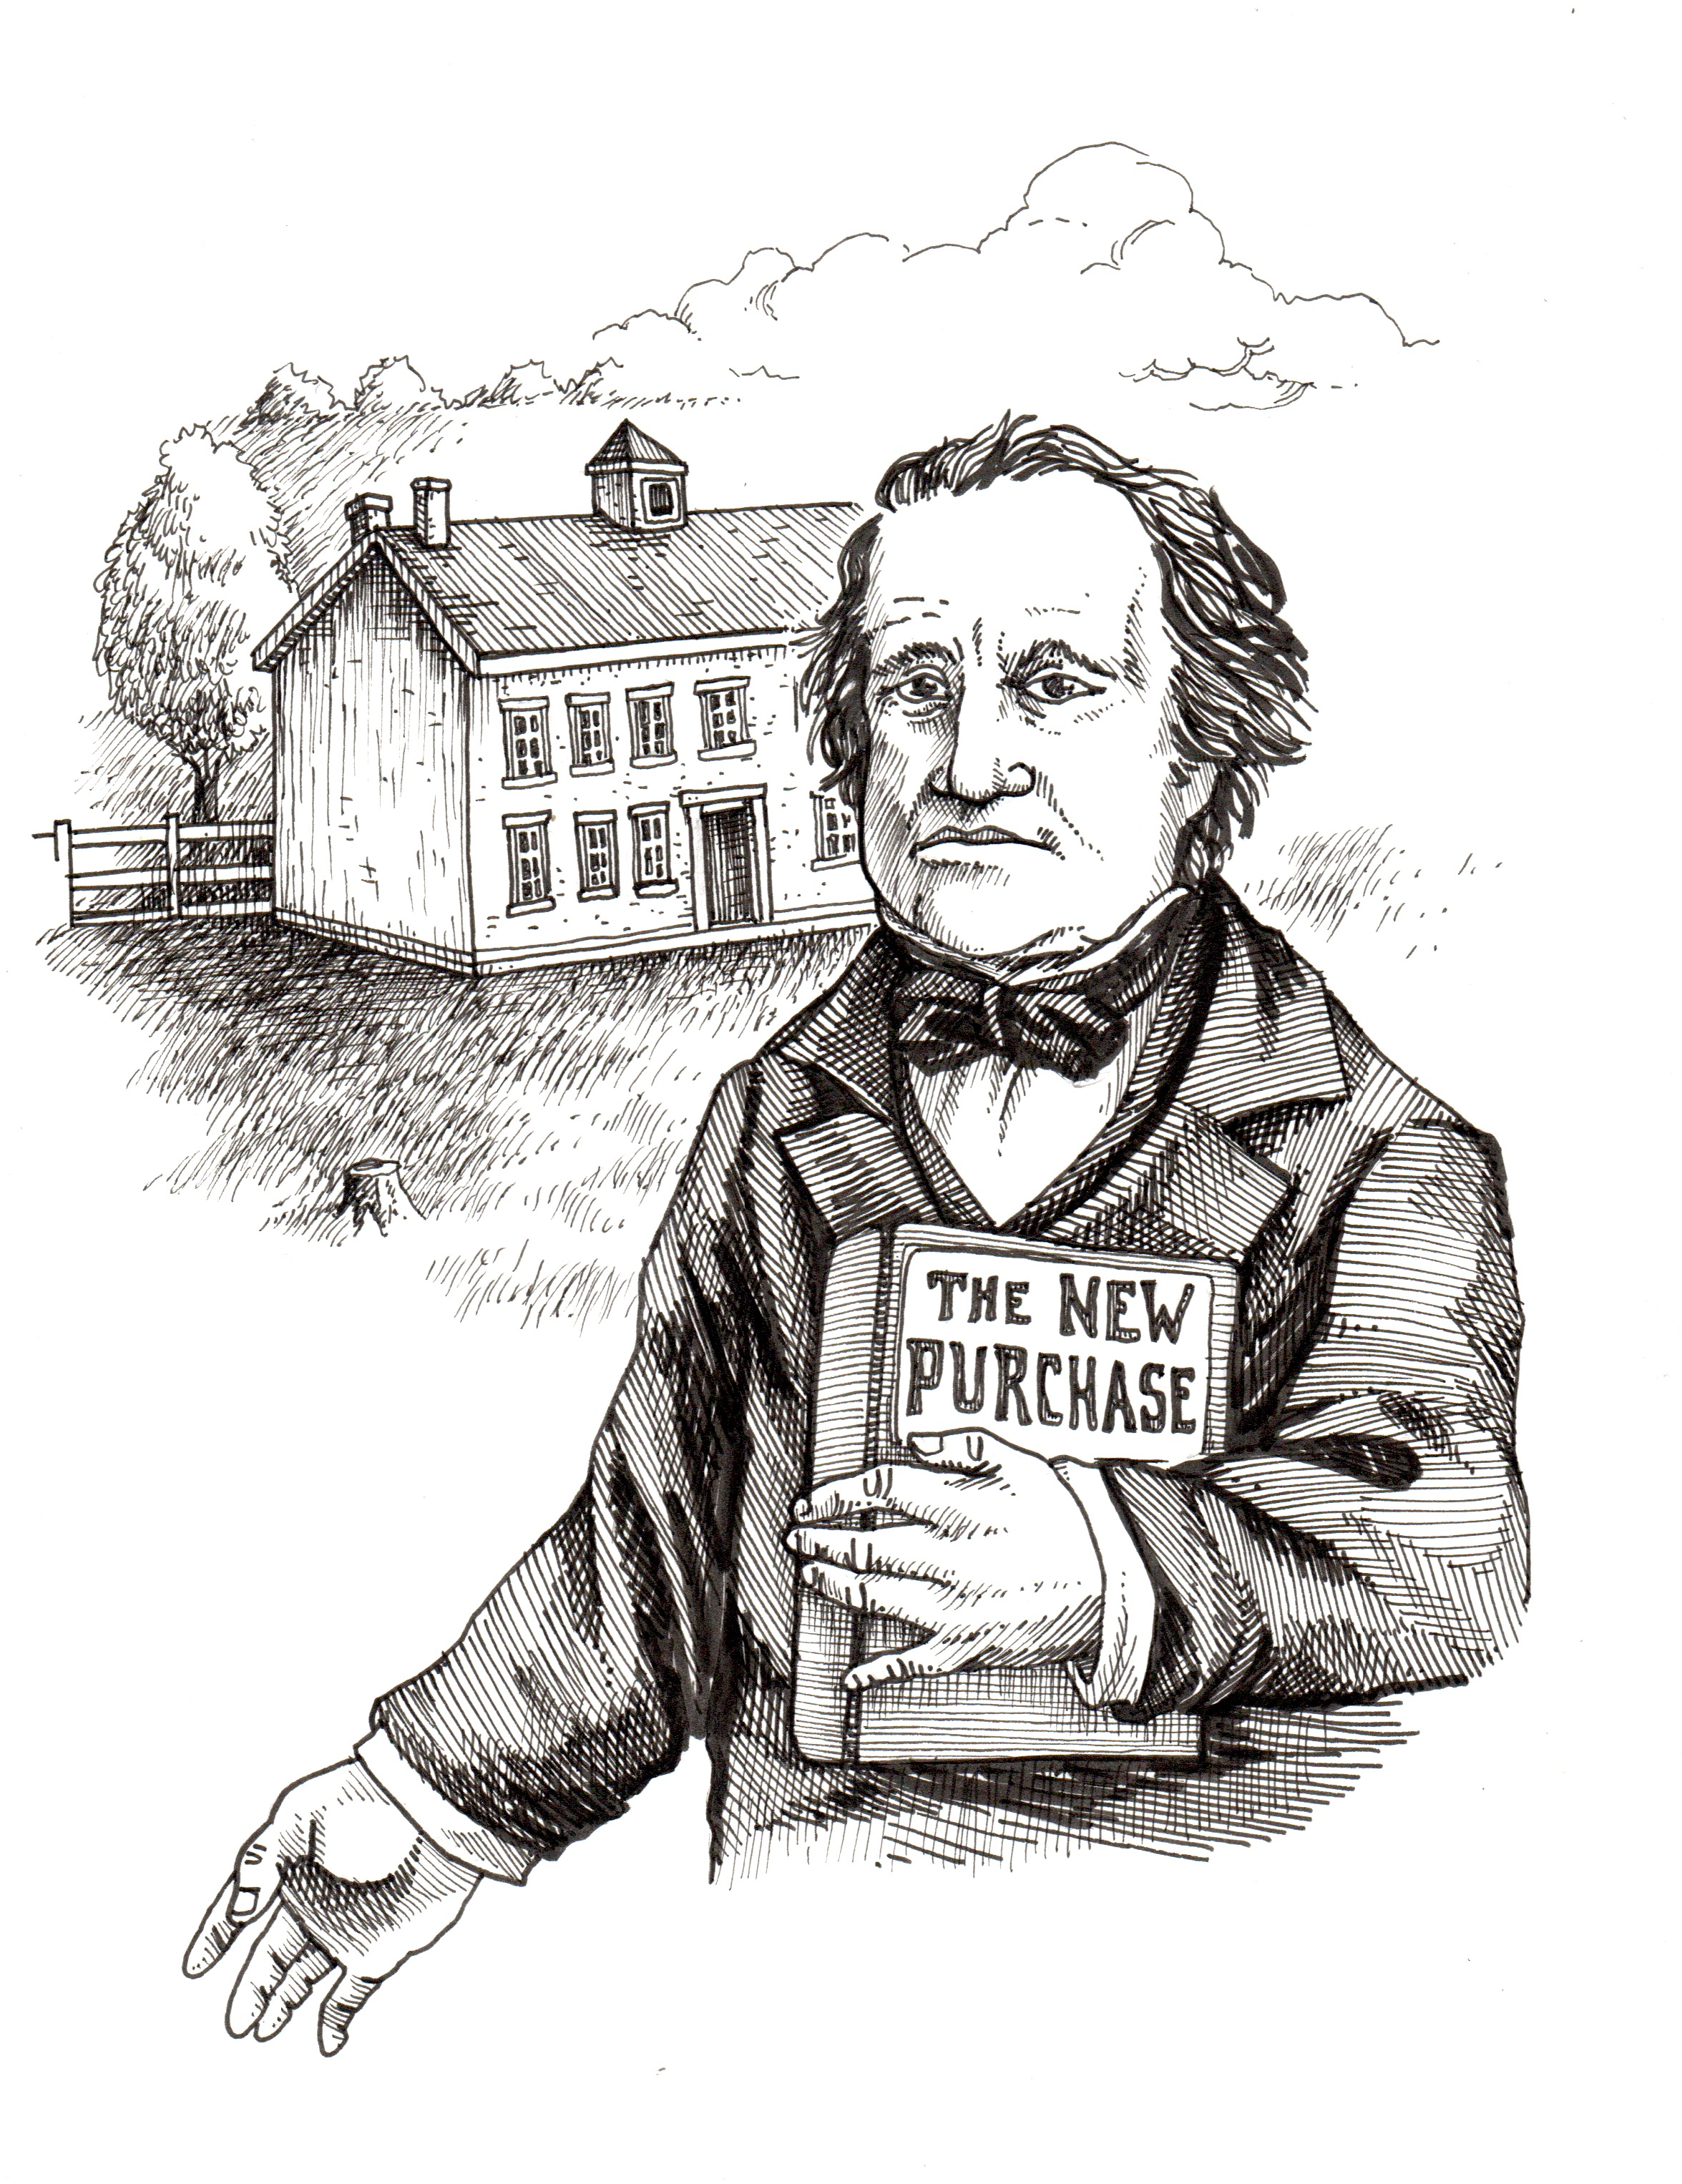
\includegraphics[width=0.6\linewidth,height=\textheight,keepaspectratio]{images/miu2.jpeg}

}

\caption{Baynard R. Hall}

\end{figure}%

\epigraph{
Human beings participate in history both as actors and as narrators. The inherent ambivalence of the word "history" in many modern languages, including English, suggests this dual participation. In vernacular use, history means both the facts of the matter and a narrative of those facts, both "what happened" and "that which is said to have happened." The first meaning places the emphasis on the sociohistorical process, the second on our knowledge of that process or on a story about that process\ldots{}. The inability to step out of history in order to write or rewrite it applies to all actors and narrators.}
{
\parbox{.75\textwidth}{\raggedleft---Michel-Rolph Trouillot, \textit{Silencing the Past: Power and the Production of History}}
}

Few people today are familiar with the Reverend Doctor Baynard Rush Hall
(1798--1863), the inaugural instructor at the progenitor of Indiana
University---the Indiana State Seminary of learning. The school was
chartered by the state legislature in 1820, and Hall served as principal
from its opening in 1825. When the tiny institution was elevated to
Indiana College in 1828, it acquired its first president, Andrew Wylie,
who also served as an instructor. In 1832, Hall left the institution
following an administrative struggle with President Wylie. The thwarting
of his ambitions motivated Hall to write a lightly fictionalized account
of his Bloomington career, \emph{The New Purchase, or, Seven and a Half
Years in the Far West}, published in 1843 in two volumes.\footnote{\citeproc{ref-hall1916a}{Hall,
  \emph{The New Purchase, or, Seven and a Half Years in the Far West},
  1916}. The New Purchase referred to the 1818 acquisition by the United
  States of the central third of Indiana from the resident Miami tribe
  and others living in the territory in the Treaty of St.~Mary's,
  conducted in Ohio during September and October 1818. Monroe County and
  Bloomington were organized in 1818.}

In addition to its endurance as a vivid description of pioneer life in
southern Indiana, the book serves as a uniquely valuable source on the
early history of Indiana University. IU's historiography has been shaped
by Hall leaving and Wylie staying for the rest of his career. Thus, the
first written accounts of institutional history describe the ``faculty
war'' ending with the termination of Hall. Ever since, the historical
role of Hall has been impoverished, relegated to the margins of IU's
institutional saga.

Hall thus was not only the first instructor, teaching Greek and Latin in
the classical curriculum, but also the first historian of the
institution. To be sure, he narrated history in a partisan manner,
outlining what he saw as Wylie's mistaken approach, but the factual
details about college life have been generally accepted. Indeed, early
IU historians wove Hall's recollections, sometimes without attribution,
into their narratives. As living memory faded over time, Hall's book
became an increasingly important historical source. Because his activity
as a historical narrator has been neglected, a closer examination of his
foundational role in the university's historiography might yield deeper
understanding.

\section{From the Metropolis to the
Frontier}\label{from-the-metropolis-to-the-frontier}

A Philadelphia native, Baynard Hall received his bachelor's degree from
Union College in Schenectady, New York, in 1820. He then attended
Princeton Theological Seminary in New Jersey, obtaining a certificate in
1823, and received a license to preach from the Presbyterian ministry.
Hall and Mary Ann Young were married in 1820, in Danville, Kentucky.
Their two young children died in 1824. Propelled by a mixture of
frontier fascination and personal tragedy, Baynard Hall and his wife
left Philadelphia in April 1824, bound for Owen County, Indiana, where
other members of the Young family had settled. Baynard was twenty-six,
and Mary Ann was twenty-eight. Completing their journey by stagecoach in
May, they arrived in Owen County, near the northern limit of white
settlement in the new state.\footnote{See
  \citeproc{ref-richardson2009a}{Dixie Kline Richardson, \emph{Baynard
  Rush Hall: His Story} (Indianapolis: Dixie Kline Richardson, 2009)}.}

Meanwhile, the Indiana State Seminary of learning was being organized by
a board of trustees. Endowed with a federal land grant, the trustees
located the school in Bloomington, a new settlement established in 1818.
The campus was carved out of the forest a few blocks south of the Monroe
County courthouse. A two-story brick Seminary Building went up, as well
as a professor's house, as ten acres of land were cleared for the
school.

In November 1824, Hall was hired by the trustees as the sole instructor
a few months before the seminary opened. Newspaper advertisements
described the young instructor: ``Mr.~Hall is a gentleman, whose
classical attainments are perhaps not inferior to any in the western
country; and whose acquaintance with the most approved methods of
instruction in some of the best universities in the U. States, and whose
morals, manners, and address render him every way qualified to give
dignity and character to the institution.''\footnote{\citeproc{ref-richardson2009a}{Richardson}.}

The description of the campus was similarly embellished: ``{[}The
buildings{]} are erected on an elevated situation, affording a handsome
view of Bloomington the county seat\ldots and also a commanding prospect
of the adjacent country which is altogether pleasant and well calculated
for rural retreats; and as it regards the healthiness of its situation,
we hazard nothing in the assertion, that it cannot be excelled by any in
the western country.''\footnote{\citeproc{ref-richardson2009a}{Richardson}.}

The Indiana State Seminary of learning opened for classes in April 1825,
with Hall welcoming around ten young men. Hall continued to serve as an
instructor for the infant institution until 1832. In those seven years,
student enrollment increased from ten to forty. The faculty was expanded
to two in 1827, with the addition of John Harney to teach mathematics,
and to three in 1829, with the hiring of Andrew Wylie to serve as
president of the institution, now known as Indiana College, as well as
to teach mental and moral philosophy, political economy, and literature.

Hall left the college under a cloud in 1832, as did Harney, because of
personal differences with President Wylie. Harboring bitter
disappointment, Hall and his wife traveled back east. Never returning to
the scene of his professional origination, the classical scholar spent
the rest of his life teaching and preaching at a series of schools and
churches in Pennsylvania, New Jersey, and New York.\footnote{\citeproc{ref-richardson2009a}{Richardson,
  180ff}.}

Hall became a published author in 1836 with a Latin grammar textbook,
which was reviewed harshly.\footnote{\citeproc{ref-hall1836a}{Baynard
  Rush Hall, \emph{Exercises, Analytical and Synthetical; Arranged for
  the New and Compendious Latin Grammar} (Bedford: Harrison Hall,
  1836)}; reviewed by \citeproc{ref-addis1839a}{Alfred Addis, {``Latin
  Grammars,''} \emph{The Literary and Theological Review} 6, no. 21
  (1839): 59--66}.} In 1843, Hall published his second book, detailing
his time in Indiana. \emph{The New Purchase} chronicled how pioneer
Hoosiers cultivated life on the frontier, including colorful
descriptions of daily activities of subsistence, transport, social
mores, and religious observance.\footnote{\citeproc{ref-hall1916a}{Hall,
  \emph{The New Purchase, or, Seven and a Half Years in the Far West},
  1916}.} The book's title was the common name of the middle third of
Indiana, after resident Indian tribes ceded their land to the United
States in the Treaty of St.~Mary's. The book has defied easy literary
categorization: written as a nonfiction composition, it was presented as
a quasi-fictive work.\footnote{The book was referred to as
  ``quasi-fictive'' by \emph{The Oxford Companion to American
  Literature} in 1983.} It contains aspects of autobiography, memoir,
and travelogue, leavened with personal diatribes directed against Wylie.

To tell his side of the story, Hall adopted an unusual approach. The
cutting satire that bordered on defamation in his statements pertaining
to Wylie motivated Hall to invent names for characters and places in
\emph{The New Purchase}. Since he was both the narrator and the chief
protagonist, he devised twin alter egos, identifying pseudonyms for the
author, Robert Carlton, Esq., and for the professor, Reverend Charles
Clarence. Carlton was also given the role of trustee (which Hall was
not).

The preface is a dialogue between Carlton and Clarence about history,
fiction, and truth. Regarding the contents of the book, Carlton
estimates ``that the Truth is eight parts out of ten, the Fiction only
two:---that the Fiction is mainly in the colouring and shading and
perspective\ldots in the aggregation and concentration of events, acts,
actors\ldots that the Chronology of the whole and the parts is in need
of some rectification.''\footnote{\citeproc{ref-hall1916a}{Hall,
  \emph{The New Purchase, or, Seven and a Half Years in the Far West},
  1916, xvii}.}

In discussion about its title, Carlton suggests to Clarence,
``Whereabouts? or Seven and a Half Years in a New Purchase of the Far
West; being a Poetic Dream at Sun Rise, with a Prosaic Reflection as Sun
Set---a Novel-History, and a Historic-Novel.'' Clarence objects,
shortening the title to the published version. In the same vein, Carlton
wants to add a ``little scrap'' of Latin---\emph{alter et idem} (``one
and the same'') and \emph{per multas aditum} (``through many paths'').

As a historical memoir, \emph{The New Purchase} has had singular value
as a narration of the early years of the institution by a main
historical actor. But the fictive names of individuals and places, and
the lack of a dependable chronology of events, have created interpretive
problems. Evidently, Hall was determined to publish an account where the
line between fact and fiction was vague, one that contained accurate
descriptions of the places and people he encountered during his sojourn
on the frontier of settlement but also infused with his private opinions
and feelings. Perhaps he took this literary approach in order to process
and redeem his young adulthood---and to protect himself from potential
charges of libel. At its publication, \emph{The New Purchase} was read
as an account of pioneer life in Indiana. For the people of Bloomington,
it also contained a fascinating account of the early operation of the
seminary and college, still less than two decades old. Some in
Bloomington were scandalized by Hall's airing of the college's dirty
laundry; others might have been secretly gratified. In the eastern
market, the book sold well, and the initial run of one thousand copies
eventually sold out.

\section{An Urtext}\label{an-urtext}

In \emph{The New Purchase,} Hall described the situation that led to his
eventual termination. The three faculty members---Hall, Harney, and
Wylie---shared much in common, including an allegiance to the
Presbyterian faith and a belief in the power of classical education.
Harney and Hall were more traditional, however, and hewed to the method
of rote learning, whereas Wylie was more open to expanding the classical
curriculum. They also differed on questions of managerial authority and
student discipline. With the coming of Wylie, who was older and had more
administrative experience, battle lines soon emerged.

For the nearly four years of the seminary's operation, Hall and Harney
had accomplished the simple administrative tasks required. However,
after the infant institution became a college, Wylie came in as
president (fleeing an untenable situation at Washington College in
western Pennsylvania) and took over administration. Complicating
matters, Wylie brought several students along with him, and friction
developed between students already in residence---so-called
``natives''---and the Pennsylvania transfers, termed ``foreigners.''

In keeping with his satirical intent, Hall invented the name
``Bloduplex'' for Wylie, to signify ``a person that could blow hot and
cold with the same breath,'' and introduced him with a rhetorical
flourish: ``We now introduce a very uncommon personage, a most powerful
prodigious great man, the first of the sort beheld in the New
Purchase---the very Reverend Constant Bloduplex, D.D.---in all the
unfathomable depths of those mystic letters.''\footnote{\citeproc{ref-hall1916a}{Hall,
  477, 480}.}

In describing Wylie's scholarly accomplishments, Hall wrote:

\begin{quote}
His talents were good; his acquirements respectable especially in
Classics, Antiquities, History, and Literature in general; ---still they
were not uncommon. In Mathematics and Sciences, we cannot state his
attainments; and simply because we never discovered them---yet he must
have gotten beyond arithmetic, since Clarence {[}Hall{]}, in return for
aid in Greek, did gratefully assist the Doctor in Algebra. Harwood
{[}Harney{]}, indeed, thought the President's attainments in such
matters inconsiderable; but then Harwood was Professor of Mathematics
and may have expected too much. At all events the President set no great
value on these matters, making himself merry at Clarence's expense, on
accidentally discovering that this gentleman was studying Mathematics
under the guidance of his friend Harwood, while Harwood read Latin and
Greek with Clarence.\footnote{\citeproc{ref-hall1916a}{Hall, 486}.}
\end{quote}

Underscoring Wylie's exaggerated portrait, Hall explicitly stated: ``We
must say that Bloduplex is really a fictitious character!''\footnote{\citeproc{ref-hall1916a}{Hall,
  488}.}

Hall went on to analyze the character of the president:

\begin{quote}
As a companion, no man \emph{could} be more agreeable than our
President. It was this led our young Professors to unbosom
{[}\emph{sic}{]} in his presence---and even when, in an unguarded
moment, the President remarked---\emph{proton pseudos}, to imagine all
sorts of wickedness and chicanery in all others; and then to combat all
with such weapons as he fancied they were using or would use against
him!\footnote{\citeproc{ref-hall1916a}{Hall, \emph{The New Purchase, or,
  Seven and a Half Years in the Far West}, 1916, 486--87}. \emph{Proton
  pseudos} refers to a wrong assumption or error in premise.}
\end{quote}

The verbal portrait was not all negative: ``Doctor B. was an excellent
preacher, and a still better lecturer, whether is regarded the matter or
the manner: and some of his pulpit exhibitions were surpassingly
fine.''\footnote{\citeproc{ref-hall1916a}{Hall, 487}.} Admiring his
adroitness in ``ecclesiastical combats,'' Hall explained that Wylie's
success was due to his ``Phrenological organization.''\footnote{\citeproc{ref-hall1916a}{Hall,
  487}.} ``My own opinion is, President B. owed most of his
victories---and some of his defeats---to his Wonderful Religious
Experience! which in the stereotyped crying places always when
\emph{first} heard inclined \emph{weak} believers to his side!'' But
upon repetition, most people saw through the act, the narrator
averred.\footnote{\citeproc{ref-hall1916a}{Hall, 487--88}.}

Alter ego professor Clarence analyzes why the president dislikes the
professors, enumerating a list of probable reasons:

\begin{quote}
1.~His jealousy of equals, and suspicious and untrustful temper: 2. His
determination for a very low grade of studies---especially in
Mathematics, and even in Classics,---he being resolved to level down and
not up: 3. His love of ease, and wish to get along with a relaxed, or
rather no discipline: 4. His using discipline as an instrument of
avenging himself on students disliked by him: 5. His domineering and
tyrannical temper: 6. His prying disposition, by which he was led to
have spies in the professors' classes, and to watch when they came and
went to and from duties. \&c.: 7. His desire to make room for former
pupils and relatives: 8. His erroneous theology.
\end{quote}

Summarizing the list of grievances, the text continues:

\begin{quote}
Hence, without consulting his peers, nay, contrary to their known wishes
and earnest remonstrances, he tried to discipline students at will and
to suspend and dismiss; he permitted some to be graduated, and who now
hold imperfect diplomas, signed with his sole name: and he
\emph{commanded} what the Professors should and should not do, and what
teach, and how, answering their arguments with insult and derision, and
threatening to stamp them and the trustees also under his feet! He
pretended to think, and dared to assert, that the discipline of a
College was of right a President's special duty, ---and teaching, the
Professors'. And, therefore, he rudely, on several occasions,
contradicted his Faculty in public, and aimed to consider and treat them
as boys!\footnote{\citeproc{ref-hall1916a}{Hall, \emph{The New Purchase,
  or, Seven and a Half Years in the Far West}, 1916, 489}.}
\end{quote}

Continuing in the same vein, Hall ended the section with speculation
about the president's motivations, including the possibility of mental
illness. In addition to criticism of Wylie, the text describes the
organization and operation of the seminary, which became increasingly
valuable historical source material.

After he introduced the major characters, Hall narrated a mystery that
was the proximate cause that led to his termination: In his recitation
room before class, Hall found an unsigned letter tucked into his pocket
edition of Virgil and read it. It accused him of being an indolent and
ineffective teacher and advised the professor to resign. The letter was
sealed with wax that bore the imprint of Wylie's desk key, so Hall
naturally thought that the president was the author. His colleague
Harney and his wife, Mary Ann, agreed with that surmise after they read
the letter. They compared older letters written by Wylie for
corroboration and discovered ``the most remarkable similarity, as to the
hand---the style---the words---the expressions---was apparent: nay, in
some things, was an identity.''\footnote{\citeproc{ref-hall1916a}{Hall,
  493}.}

Harney advised Hall not to resign, however, without seeing President
Wylie first. Hall described their meeting:

\begin{quote}
The letter was taken by the President, but \emph{not read all carefully
and indignantly over}, as by the others! And yet, at a glance, he
learned all its items, and that so well, as to talk and comment on them!
But still, after what he designed should pass for a searching scrutiny,
in a moment he exclaimed,---``I \emph{know} the hand writing---it is
\emph{Smith's}!''\\
``How you relieve me, Doctor Bloduplex,'' said Clarence; ``Harwood was
right to prevent me from sending in my resignation.---I shall
continue---''\\
``Mr.~Clarence,'' replied the President, ``Smith, \emph{I} know, is your
bitter enemy; and I am \emph{told} you have many more, and especially
among the \emph{young gentlemen} that came with me: now, this shows a
state of great unpopularity, and \emph{I do candidly advise, all things
considered, that you had better resign!!}''\\
``Doctor, pardon me, my first belief is returned---I know the author of
this letter, and it is \emph{not} Smith.''
\end{quote}

Later in the passage, Hall shared his strong impression that Wylie wrote
the letter:

\begin{quote}
``Dr.~Bloduplex, from my inmost soul I do hope you may remove my
suspicion,---but I much fear that you yourself are the author of this
letter!''\\
``I!---the author! how could you ever entertain so unjust a
suspicion?''\\
``God grant, sir, it be unjust---but I will give you the grounds of my
suspicion.''\\
``Name them, sir,---I am curious and patient.''\\
Here Clarence went over all that the reader has been told, but to a much
wider extent, and with many arguments and inferences not now narrated;
and then spread out the Doctor's own letters, to be compared with the
anonymous one. Upon which the Doctor said:\\
``Well, Mr.~Clarence, there is no resemblance between them, or but very
little.''\\
``But is there not \emph{some}? Has not the writer tried to imitate your
hand---your style---your very grammatical peculiarities?''\\
``It does, maybe, seem a little so---''\\
``It does, indeed, Doctor Bloduplex; and now look here!---\emph{the seal
is stamped with the key of your desk!}''\\
Here the President coloured; of course in virtuous indignation and
surprise at such roguery, and in some little confusion exclaimed:---\\
``The wicked dogs! they have \emph{stolen} the \emph{key} of my
desk!''\\
Clarence was here affected to tears; that one the other day almost loved
and trusted as a father could be by him no longer so regarded\ldots.\\
``Only assure me, Doctor, on your word of honour and as a Christian that
\emph{you} did not do this base action, and even now will I burn this
letter in this very fire---(it was a cold day)---before your face.''\\
``Mr.~Clarence,'' said he ``I solemnly declare I did not write this
letter; but stay, do not burn it---let me have it and I will try and
find the writer.''
\end{quote}

Still mystified by the poisonous letter, Hall narrated both his
disbelief and his surprising reaction:

\begin{quote}
Of course, then, the letter was not written by the Reverend Constant
Bloduplex, d.d.---for he had the best right to know; and he \emph{said},
solemnly, that it was not. Yet Clarence, ``all things considered,'' did
that very week send his resignation to Dr.~Sylvan {[}trustee president
David Maxwell{]}; offering, however, to remain till the meeting of the
Board. At that the Board offered him nearly double salary to remain some
months longer till a suitable successor could be found; to which
proposal Clarence acceded.
\end{quote}

This then is the story that Hall narrated in \emph{The New Purchase}, in
which he was the primary protagonist.

The next year, 1831--32, Hall continued teaching temporarily, and the
mystery of the anonymous letter persisted. Harney became embroiled in
public controversies with Wylie over student behavior. Things escalated
so much that the two men were involved in a physical altercation in
which Wylie pushed Harney off a log spanning a mudhole. Eventually Wylie
convinced the board of trustees to terminate Harney for insubordination.
So, at the end of the 1831--32 school year, the original two professors
left, and the administration was faced with finding replacements. The
author of the anonymous letter did not come forward, leaving a chasm of
silence surrounding the initiatory event that triggered the termination
of the original faculty.

\section{A Complex Historiography}\label{a-complex-historiography}

Most of what we know about the early history of the Indiana State
Seminary and Indiana College derives from Hall's account in \emph{The
New Purchase}. There are no extant sources that bear on Wylie's or
Harney's reactions to Hall's testimony in the book. Although Hall had
ample motivation to tell his side of the story about his conflict with
the president, there is little reason to believe that he exaggerated or
made false claims about it. As a writer, Hall usually left clear
evidence of the facts of the matter at hand and his interpretation of
them. But his deliberate scrambling of chronology and his penchant for
combining separate acts have left readers puzzled. What emerges in
\emph{The New Purchase} is a protagonist trying to integrate various
aspects of his personality and come to grips with his young adulthood by
narrating his personal experiences, including his emotional reactions.

In a figurative sense, taken as a metaphor for those pioneering times,
\emph{The New Purchase} is a tale of ambition, intrigue, and
disenchantment. Each of the protagonists---Hall, Wylie, and
Harney---attempted to gain purchase on new opportunities as the state of
Indiana made halting steps toward public higher education. Although our
perspective is obscured by the passage of nearly two centuries, each of
these men, full of passion and hope, made their way to the frontier
hamlet of Bloomington to shape an infant institution. The outcome of
their contest for influence meant that their names are differentially
remembered, but all of them acquired some return for their investment of
time and energy.\footnote{One early example is found in Charles
  Blanchard, ed., \citeproc{ref-blanchard1884a}{\emph{Counties of
  Morgan, Monroe, and Brown, Indiana: Historical and Biographical}
  (Chicago: F.A. Battey \& Co., 1884)}, 478:

  \begin{quote}
  President Wylie's connection with the college proved very
  advantageous, not only to that institution, but to Bloomington and
  Monroe County. He was famed for his learning all over the East and
  South, and soon students from distant States came to Bloomington to
  place themselves under his instruction. But the sudden and permanent
  popularity of President Wylie led to bitter jealousy on the part of
  Profs. Hall and Harney, who no doubt envied him his good fortune, and
  wished for the possession of his place and honors. The unpleasantness
  ceased with the permanent departure of Hall and Harney, in 1832. The
  college flourished greatly under the management of President Wylie,
  and its influence was soon felt upon the community.
  \end{quote}}

Using \emph{The New Purchase} as an archival source for interpretations
of IU's past has generated a complex and interesting historiography.
Although the college was expanded and renamed Indiana University in
1838, its history remained confined to oral tradition until Hall's book
was published in 1843. David Maxwell and Andrew Wylie continued their
administrative service into the 1850s, although faculty turnover was
high. The deaths of Wylie in 1851 and Maxwell in 1854 were blows to the
institution, removing two key individual mainstays. Over time, the
details of their accomplishments were obscured, and collective memory
enshrined the two men as founding figures. Following the College
Building fire in 1854, Hall published a revised edition of \emph{The New
Purchase} in 1855, omitting the invective against Wylie and with it some
descriptions of the institution.

After his departure from Bloomington in 1832, Hall held a variety of
teaching posts at small academies in Pennsylvania, New Jersey, and New
York, often in combination with serving local Presbyterian
congregations. He had a remarkable career as an author, with six books
published in the two decades between 1836 and 1855. As mentioned
previously, the first, in 1836, was a Latin grammar textbook ``for the
use of primary schools, academies, and colleges.'' Seven years later,
\emph{The New Purchase} came out. It became his most successful book
and, perhaps, his most personally gratifying.

His rate of publication then dramatically increased, with another three
titles in seven years. In 1846, Hall published another blend of personal
quasi-fictive narrative: \emph{Something for Every Body: Gleaned in the
Old Purchase, from Fields Often Reaped}. Using the same pseudonyms
(Robert Carlton, Esq., and Reverend Charles Clarence) and a dialogue
structure, the book was an exchange of letters between Hall's twin alter
egos, talking about how to live a godly life. Dixie Richardson, Hall's
biographer, called the book ``an exuberant exposition of Hall's opinions
and observations on numerous subjects: theology, medicine, capital
punishment (a gallows at the edge of town indicates the community
provides its citizens safety), temperance, contemporary trends (unlike
Brooklyn writer Walt Whitman, Hall scoffs at phrenology) and in the
process he added more of his own history.''\footnote{\citeproc{ref-richardson2009a}{Richardson,
  \emph{Baynard Rush Hall}, 208}.}

Two years later, Hall published a nonfiction title, \emph{Teaching, a
Science: The Teacher an Artist}, in which he expressed his views on
pedagogy, noting in the preface, ``This book is not an experiment, but
an experience.''\footnote{\citeproc{ref-hall1848a}{Baynard Rush Hall,
  \emph{Teaching, a Science: The Teacher an Artist} (New York: Baker;
  Scribner, 1848), v}.} In 1852, riding the wave of interest created by
the publication of \emph{Uncle Tom's Cabin} by Harriet Beecher Stowe,
Hall released \emph{Frank Freeman's Barber Shop}, a novel featuring both
Black and white main characters.\footnote{\citeproc{ref-hall1852a}{Baynard
  Rush Hall, \emph{Frank Freeman's Barber Shop} (New York: Scribner,
  1852)}.}

Upon publication of the revised edition of \emph{The New Purchase} in
1855, Hall was coming to the end of a remarkable period of literary
productivity. It had been a dozen years since its original publication,
and New Albany, Indiana, publisher John Nunemacher stoked Hall's hopes
for a revival of interest in the work. After Wylie's death in 1851, Hall
felt it was unseemly to mention their conflict and so excised nearly 130
pages that gave details about the story, omitting much of the
description of the state seminary and college.\footnote{In
  correspondence about the second edition, Hall stated, ``In the work
  here and there certain words and expressions that have caused me often
  much sorrow in remembrance, and I would have given many dollars if
  they could have been blotted out. And more especially there would be
  so manifest an unkindness in reprinting a vast amount of what pertains
  to the late President of a certain college, that I would nearly as
  soon consent to have a finger taken off as to continue that''
  (\citeproc{ref-hall1855a}{Baynard Rush Hall, {``Letter to John
  Nunemacher,''} May 13, 1855}).

  Hall reminded Nunemacher that ``all of the chapters and passages in
  the second volume relative to Dr.~Bloduplex (President Wylie) are by
  all means to be discarded\ldots. This gentleman richly deserved all
  that was done to him some years ago, but he is now in the other life,
  and I hope in a better one'' (\citeproc{ref-hall1855a}{Hall};
  \citeproc{ref-banta1914a}{David D. Banta, {``History of Indiana
  University: IV. The {`Faculty War'} of 1832,''} \emph{Indiana
  University Alumni Quarterly} 1, no. 4 (1914): 369--86})} Illustrations
were added, the subtitle was shortened to ``Early Years in the Far
West,'' and the original preface was replaced with a new one, written
and signed by B. R. Hall, ``Author, \emph{Pro. Tem.}'' The frontispiece
featured an engraved portrait of Hall, identified simply as ``The
Author.'' Never resisting a didactic opportunity, Hall translated the
Latin quotations that appeared on the title page: ``\,`\emph{Alter et
idem}' means,---`\emph{pretty much of a muchness},' or in better
Saxon---`\emph{Six of one and half a dozen of the other}.' {[}`\emph{Per
multas aditum sibi sæpe figuras repperit}' means{]}---`\emph{Being
crafty he catches with guile}.' And these are the \emph{freest}
translations we are at liberty to give.''\footnote{\citeproc{ref-hall1855b}{Baynard
  Rush Hall, \emph{The New Purchase; or, Early Years in the Far West},
  2nd ed. (New Albany, IN: Jno. R. Nunemacher, 1855)}.} Appearing in a
single volume, the second edition of \emph{The New Purchase} did not
attract many new purchasers interested in reading about frontier days in
southern Indiana.

On the first of January 1863, during the Civil War, the Emancipation
Proclamation was issued. Hall was living in Brooklyn at the time,
working at the Park Institute School and assisting with services at the
Dutch Reformed Church. Later that month, Hall died a few days before his
sixty-fifth birthday. His passing merited an obituary in the \emph{New
York Times}:

\begin{quote}
As an author, as well as a teacher, he gained a wide reputation.
Dr.~Hall was distinguished by high intellectual culture and refinement,
by delightful conversational powers, to which an incessant current of
humor lent animation and brilliancy, and to which the cordial kindness
of his nature gave geniality. His life, influenced by the strongest
religious convictions, as well as by inherent charity, was spent in
labors of beneficence which were only interrupted by his final illness.
\end{quote}

In addition to misspelling his middle name as ``Rust,'' the obituary
included a mischaracterization in the recitation of his positions:
``Pastor of a Church and President of a College in Bloomington, Ind. for
some years.''\footnote{\citeproc{ref-nytimes1863}{{``Obituary: Baynard
  Rust {[}\emph{{s}ic}{]} Hall,''} \emph{New York Times}, January 27,
  1863, 5}.} The first IU professor passed into historical memory,
joining the first president and the first trustees board president.

\section{Gathering the ``Historical
Catalog''}\label{gathering-the-historical-catalog}

In 1881, the IU Board of Trustees asked longtime professor Theophilus
Wylie to prepare a written ``historical catalog'' for the university.
The university had been granting diplomas for a half century, and there
was a felt need to summarize the history of the institution in a
permanent document. Hired in 1837, Wylie was the seventh person
appointed to the faculty; he was also Andrew Wylie's cousin. Wylie
started writing to alumni and former faculty to gather information.
Trustee David Banta, a former judge and county historian, became
president of the trustee board in 1882, and he also started writing to
former members of the university's academic community for
information.\footnote{\citeproc{ref-banta1881a}{D. D. Banta, \emph{A
  Historical Sketch of Johnson County, Indiana} (Chicago: J.H. Beers \&
  Co., 1881)}; \citeproc{ref-mccaslin1888a}{William McCaslin and D. D.
  Banta, \emph{History of Johnson County, Indiana} (Chicago: Brant \&
  Fuller, 1888)}.}

Among the people Professor Wylie contacted was his relative Andrew Wylie
Jr., the eldest son of the former president and an 1832 graduate of
Indiana College. He served as a federal judge of the Supreme Court of
the District of Columbia. Professor Wylie was seeking information about
Judge Wylie's father and inquired about the anonymous letter that
Professor Hall referred to in \emph{The New Purchase}: ``I have never
thought it possible that he could have written it, \& I would {[}inquire
if?{]} you know certainly that \& positively that it was not written by
him, not as I know it {[}from?{]} being morally certain that he did not
\& could not have written it. Please inform me, so that from positive
knowledge I might contradict it. I do not mean in the published
catalogue, for I think it would be better to ignore all disagreeable
things in such a publication.''\footnote{\citeproc{ref-wylie1881a}{Theophilus
  Wylie, {``Letter to Judge Andrew Wylie,''} July 18, 1881.
  IUA/C202/B5/F Letters relating to history}.}

Banta wrote to Matthew Campbell, a member of the class of 1834 and a
former instructor in IU's Preparatory Department, who replied in detail
about his memories. Regarding the anonymous letter, he wrote, ``I know
that Judge Wylie (who now strongly resembles his father tho' he was
nothing like him 50 years ago) w{[}oul{]}d acknowledge the anonymous
letter as his own. And yet I judge he never so acknowledged it to his
father. Ask him.''\footnote{\citeproc{ref-campbell1882a}{Matthew
  Campbell, {``Letter to David Banta''} (Indiana University
  Archives/C112/B1, December 25, 1882)}.}

Unbeknownst to Campbell, Banta had received a letter from Judge Wylie a
short time earlier, admitting that he was the author of the anonymous
letter.

\begin{quote}
Washington Dec 17, 1882\\
D.D. Banta, Esq.

Dear Sir: Your letter date 7\textsuperscript{th} inst. was duly received
and would have had earlier attention but for the pressure of official
and other duties. The anonymous letter to which you refer was written by
me without the knowledge, suggestion, remotest hint, or suspicion on the
part of my Father. I was at that time a boy of sixteen years. The
anonymous note to Mr.~Hall contained no more than the almost universal
opinion of the students. He was indolent, careless, superficial and
shamefully neglectful of his duties. Both he and Mr.~Harney had been
professors in the college for several years previous to Father's
election as its first president, and were jealous of him, on that
account, as well as for other obvious reasons. The letter was the deed
of a boy, a small affair, and ought to have been so regarded. Mr.~Hall
\& Mr.~Harney, however, declared that it was my Father's hand,
disguised, would accept no denial, would hear no explanation, and
refused consent that an investigation should be made by the faculty.
Father offered to have every student examined, on honor, and pledged
himself that whoever should be found to have written the letter he
should be expelled. Hall \& Harney declined to have the investigation
made, but continued to circulate this false charge throughout the state,
along with others equally unfounded. Father became indignant, and
thenceforth treated them as personal enemies and wilful {[}\emph{sic}{]}
slanderers. It was an ill considered {[}\emph{sic}{]} thing on my part
to write such a letter, but every word of it was true, and I had no idea
that it was to create so much trouble. After the trouble was
created{[},{]} I felt impelled to come out and avow its authorship, but
was restrained from so doing, by the consideration that such an avowal
would be used by H. \& H. as proof that their charge was substantially
true, and that the letter, if not written by the hand of Dr.~Wylie, was
written by his son, at his dictation; and I retained the secret for
years afterwards, even from my Father. I do not now pretend to claim
that my conduct in this respect was either wise or brave. A man of
mature mind and experience would have adopted the other course. I do not
know whether or not my Father even ever prepared such a written account
of the matter as that you refer to: I never saw, or heard of it, if he
did. I have always regarded, as do now look upon the affair as beneath
the serious consideration of sensible people, except for the slander to
which it gave rise to and the annoyance it gave to my Father, whose
nature revolted at the suggestion of a meanness and was ever at warfare
with all sorts of pretenders and rascals.

{[}Signed{]}\\
Andrew Wylie
\end{quote}

With the letter in hand, Banta confirmed the identity of the anonymous
writer of the letter that had led to Hall's termination a half century
before. Surviving records do not tell whether he shared the knowledge
with Theophilus Wylie and other individuals, but he suppressed the
information when he prepared a speech on ``The Faculty War'' presented
ten years later.

In mid-July 1883, amid a driving rainstorm, Indiana University suffered
another calamity as Science Hall was struck by lightning and consumed by
the resulting fire. Science Hall housed IU's extensive scientific
collections, including the Owen Cabinet of natural history and Professor
David Jordan's fish specimens, as well as the library and administrative
records---nearly all of which was destroyed. Unlike the 1854 campus
fire, it did not cripple the university, but it was the proximate cause
of relocating operations to a more commodious site on the eastern
outskirts of Bloomington. About a year later, a new president was
chosen. The new Dunn's Woods campus was ready in 1885, presided over by
the former biology professor Jordan, who oversaw major changes in the
curriculum that accompanied the move.

The loss of another tranche of university records made the historical
catalog project more difficult but increased motivation for its
completion. Professor Wylie and trustee president Banta continued to
push forward in the tedious gathering of data from the alumni body.
Wylie reached emeritus status in 1886, and though now in his
mid-seventies, he remained dogged in his pursuit of the project. Banta
was working closely with the new president, Jordan, making pleas for
more state support and trying to improve the university. An important
way to document the past, the historical catalog was seen as a necessary
background to the current revivification, which added the promotion of
research to the existing goals of equipping students with useful skills
in the context of liberal arts education.

While research continued for the historical catalog, in 1889 President
Jordan announced a day dedicated to the founders of IU---called
Foundation Day. Its centerpiece was a historical address by Banta, who
soon would retire as trustee president to take up the deanship of the IU
School of Law. In keeping with the oral tradition and hewing to the
storyline promoted by David Maxwell, the inaugural leader of the
trustees, Banta started with ``The Seminary Period (1820--1828),'' which
dealt with the state's first effort to provide higher
education.\footnote{See \citeproc{ref-mcmains2010a}{Howard F. McMains,
  {``The Indiana Seminary Charter of 1820,''} \emph{Indiana Magazine of
  History} 106 (2010): 356--80}.} Reading from a text prepared for the
occasion, he described the legislative history of the Indiana State
Seminary of learning and its first instructor:

\begin{quote}
While the General Assembly was legislating the seminary into existence,
a young man, destined to be its first professor and to stay with it
through its seminary life, and to be with it when it passed up into the
Indiana College, and finally to leave that college a disappointed and
embittered man and write a book maligning his enemies and making sport
of his friends, was taking his last year's course of lectures at Union
College, under the celebrated Dr.~Nott. This young man was Baynard R.
Hall. After receiving his first degree at the commencement of 1820 at
Union, he went to Princeton where he studied theology, after which he
was ordained a minister of the Presbyterian church. Returning to
Philadelphia, his natal city, at the close of his theological studies,
he married and soon after set out with his bride for the New
Purchase.\footnote{\citeproc{ref-banta1914b}{David D. Banta, {``History
  of Indiana University {I}: The Seminary Period (1820--1828),''}
  \emph{Indiana University Alumni Quarterly} 1, no. 1 (1914): 3--24},
  quote on 13.}
\end{quote}

Banta mentioned Hall several times during his speech and used
information derived from \emph{The New Purchase}, sometimes without
attribution. He also speculated, without evidence, that Hall came to
Indiana because of the seminary.

On the following Foundation Day, in 1890, Banta continued with the early
history of the institution, ``From Seminary to College (1826--1829).''
He detailed its legislative history and the coming of Andrew Wylie as
its inaugural president. Members of the class of '90 presented
\emph{Scenes from the New Purchase}, an original play adapted from
\emph{The New Purchase}. Composed of four scenes depicting Hall's
sojourn: travel from Louisville to Bloomington, his hiring by the board
of trustees, the first meeting of the first class, and the protest over
Harney's religious faith (Presbyterian) being the same as Hall's. The
play featured handmade costumes, and a prologue read by Samuel B.
Harding, a history professor.\footnote{See the description of the second
  staging of the play twenty-five years later, at the 1915 alumni
  reunion: \citeproc{ref-iuaq1915a}{{``The 1915 Commencement,''}
  \emph{Indiana University Alumni Quarterly} 2, no. 3 (1915): 282,
  286--87}.}

The historical catalog, titled \emph{Indiana University, Its History
from 1820, when Founded, to 1890}, was finally ready for publication in
1890. Banta contributed the chapter ``The Indiana Seminary,'' which was
shortened from his Foundation Day address. In it, he described the first
professor:

\begin{quote}
The choice could hardly have fallen upon a worthier man. His academic
education he had received at Union College and his theological at
Princeton. He was an excellent classical scholar and a persuasive and
sometime eloquent preacher. As a teacher he was enthusiastic, faithful
and painstaking. Into the frontier life of the White River settlement,
in which his lot was cast for a time after he first came to the State,
he entered with a zeal that soon brought him to know all its
peculiarities, a knowledge that stood him many a good turn while at the
head of the State seminary.\footnote{\citeproc{ref-wylie1890a}{Wylie,
  \emph{Indiana University, Its History from 1820, When Founded, to
  1890, with Biographical Sketches of Its Presidents, Professor and
  Graduates, and a List of Its Students from 1820 to 1887}, 38--46},
  quote on 43.}
\end{quote}

Banta described the frontier skills Hall acquired and his interest in
pioneer ways.

Two years later, in 1892, Banta presented his fourth Foundation Day
address, entitled ``The `Faculty War' of 1832.''\footnote{\citeproc{ref-banta1914a}{Banta,
  {``History of Indiana University,''} 1914}; quote on 373. Republished
  in \citeproc{ref-woodburn1940a}{Woodburn, \emph{History of Indiana
  University}, 1940, 78--97}.} He described the main
protagonists---President Andrew Wylie, Professor Baynard Hall, and
Professor John Harney---and concluded with a summary of their
characters: ``Men admired the tall, graceful, grave, stately-stepping,
and dignified Wylie. Men loved the blue-eyed, jolly, laughing,
easy-going Hall. Men feared the erect, precise, nervous, heavy-jawed,
firmly-stepping, neatly dressed, military-looking Harney.''\footnote{\citeproc{ref-woodburn1940a}{Woodburn,
  \emph{History of Indiana University}, 1940, 82}. They were all dead by
  that time, so he relied on other sources.}

Banta went on to narrate a key element of the story---the anonymous
letter: ``Some time toward the close of the collegiate year of
1830--1831, probably in September---which was nearly two years after
Dr.~Wylie came---Professor Hall found in his `pocket Virgil, left as
usual on the mantel of his recitation room,' an anonymous letter, which
taxed him the very plain language with the same charges current among
the `foreign' students---incompetency and neglect of duty---and demanded
his resignation.''\footnote{\citeproc{ref-woodburn1940a}{Woodburn, 84}.}

Hall was convinced that Wylie wrote the letter, and his colleague Harney
agreed, but Wylie ``solemnly and indignantly denied its
authorship.''\footnote{\citeproc{ref-woodburn1940a}{Woodburn, 85}.}
Banta stated unequivocally, ``And yet Dr.~Wylie did not write that
letter. It was written by a Pennsylvania student, `without,' as he
himself says, `the knowledge, suggestion, remotest hint or suspicion' on
the part of Dr.~Wylie.''\footnote{\citeproc{ref-woodburn1940a}{Woodburn,
  85}. Banta quoted from Andrew Wylie Jr.'s letter but did not identify
  him by name.} Banta quoted Hall's account of his resignation in
\emph{The New Purchase} but went on to discuss Hall's actual letter,
which he saw as part of the ``old record'' that was destroyed by the
1883 campus fire and in which Hall cited dissatisfaction.\footnote{\citeproc{ref-woodburn1940a}{Woodburn,
  85}.}

For his general storyline, Banta depended on the description of the
episode in \emph{The New Purchase}, even quoting the book without
citation, but augmented by his inquiries the decade before. He did not
reveal the plain truth that the junior Andrew Wylie, now a federal
judge, had written the letter, only that a ``Pennsylvania student'' was
the author. Obliquely, he did disclose Matthew Campbell's understanding
that Wylie, a fellow classmate in the 1830s, was the writer.\footnote{Banta
  described Campbell: ``who was a student here at the time the letter
  was written, and who for forty years kept the secret of the writer.''
  \citeproc{ref-woodburn1940a}{Woodburn, 84}. ``Forty years'' probably
  refers to the publication of \emph{The New Purchase} in 1843 and the
  1882 receipt by Banta of letter from Andrew Wylie Jr.~admitting
  authorship. That raises the intriguing questions of who else knew the
  secret in the 1830s, how it was spread following the 1882 letter, and
  why it remained hidden in the archival files for decades.}

Thus, Banta's narrative became the latest writing on the subject,
incorporating Hall's 1843 account but providing a new interpretation
that emphasized its effect on the university. Judging that ``neither
side was without fault,'' he eschewed assigning blame but concluded
``their personal controversy worked a grievous wrong to the
institution.''\footnote{\citeproc{ref-woodburn1940a}{Woodburn, 96--97}.}
This rewriting of institutional history obliterated Hall's original
motivation by incorporating his account for new purposes.\footnote{Cf.
  Merton's dictum, ``obliteration by incorporation.'' See
  Chapter~\ref{sec-three}.}

\section{Into the Twentieth Century}\label{into-the-twentieth-century}

In 1902, the \emph{Indianapolis News} published a retrospective review
of \emph{The New Purchase} with fresh insight into its historical value:

\begin{quote}
As a volume curiously expository of early Indiana, it is also a volume
curiously expository of Dr.~Baynard Rush Hall. Regarded as a literary
boomerang, the printed word far outranks the pen or the sword\ldots.To
the painful surprise of Dr.~Hall and his New Albany publishers, the new
edition of ``The New Purchase'' created no furor in the book world, East
or West. The book, however, sold slowly for almost half a century; and
now a copy of the 1855 edition is almost as unobtainable and as great a
book curio as one dated 1843. With all its faults, and in spite of
Indiana's resentment of its unjust caricature, the human interest of
``The New Purchase'' will long maintain it, as Dr.~Hall pronounced it,
an ``Indiana classic.''\footnote{\citeproc{ref-carleton1902a}{Emma
  Carleton, {``About the New Purchase,''} \emph{Indianapolis News}, May
  16, 1902, 10}.}
\end{quote}

With no mention of its role as an early account of the origins of
Indiana University, the review underscored its value in American
literary and social history.

In 1913, IU historian James Woodburn published a commentary on \emph{The
New Purchase}, inaugurating another phase in its literary
historiography. Appearing in the \emph{Indiana Magazine of History}, it
was an address prepared for the History Society of Wabash College and
was also read before other county history groups. Woodburn emphasized
Hall's connection to the new state seminary and his literary ambitions
before launching into a review of frontier life as depicted in the
volume. He spoke about Hall's descriptions of native speech patterns,
social life, amusements, and politics, among other topics. Despite the
presence of ``the benighted and the indifferent,'' Woodburn spoke about
the pioneer spirit that Hall brought to life: ``But let us remember that
among the rank and file of struggling Hoosiers in the new commonwealth
there were others who hailed the prophecy and the promise of a better
day; who gave of their toil and meagre substance to truth, to religion,
to learning and education, and who were ready to dedicate to the
upbuilding and higher intelligence of their State, their lives, their
fortunes and their sacred honors.''\footnote{\citeproc{ref-woodburn1913a}{James
  A. Woodburn, {``Local Life and Color in the New Purchase,''}
  \emph{Indiana Magazine of History} 9, no. 4 (1913): 215--33}, quote on
  233.} In keeping with Woodburn's professional commitments, he advised
the audience of students and residents in his conclusion: ``One of the
uses of history is to remind us not only of our unpaid obligation to the
past, but of our never-ending obligation to the future.''\footnote{\citeproc{ref-woodburn1913a}{Woodburn,
  233}.}

As IU enrollments had grown steadily since the late nineteenth century,
the ranks of alumni had followed suit. To increase communication with
that constituency, the \emph{Indiana University Alumni Quarterly} was
launched in 1914. It contained a mix of university news items, feature
articles, and alumni notes. It soon became the journal of record for
contributions to IU history, with the help of Professor Woodburn and the
editor, Ivy Chamness. Banta's annual addresses on Foundation Day,
presented from 1889 to 1894, were published in the first six issues of
the \emph{Alumni Quarterly}, including ``The Seminary Period'' and ``The
`Faculty War' of 1832,'' further disseminating his version of the
story.\footnote{\citeproc{ref-banta1914b}{Banta, {``History of Indiana
  University {I}''}}; \citeproc{ref-banta1914c}{David D. Banta,
  {``History of Indiana University: II: From Seminary to College
  (1826--1829),''} \emph{Indiana University Alumni Quarterly} 1, no. 2
  (1914): 142--65}; \citeproc{ref-banta1914d}{David D. Banta, {``History
  of Indiana University: III: The New Departure (1829--1833),''}
  \emph{Indiana University Alumni Quarterly} 1, no. 3 (1914): 272--92};
  \citeproc{ref-banta1914a}{Banta, {``History of Indiana University,''}
  1914}; \citeproc{ref-banta1915a}{David D. Banta, {``History of Indiana
  University: V: From College to University (1833--1838),''}
  \emph{Indiana University Alumni Quarterly} 2, no. 1 (1915): 5--17};
  \citeproc{ref-banta1915b}{David D. Banta, {``History of Indiana
  University: VI: Perils from Sectarian Controversies and the
  Constitutional Convention (1838--1850),''} \emph{Indiana University
  Alumni Quarterly} 2, no. 2 (1915): 99--110}.} Woodburn followed with
eight articles, published from 1915 to 1917, dealing with the
university's history from 1840 to 1860.\footnote{\citeproc{ref-woodburn1940a}{Woodburn,
  \emph{History of Indiana University}, 1940}.}

Meanwhile, Professor Woodburn convinced Princeton University Press to
republish the 1843 edition of \emph{The New Purchase}, long since out of
print, as a contribution to the 1916 centennial commemoration of
Indiana's statehood. Woodburn wrote an introduction to the volume and
some explanatory footnotes. He enthused, ``This work has been pronounced
`one of the best books ever written concerning life in the West,'\,''
adding, ``There is certainly no more valuable book on early Indiana.''
Woodburn quoted his erstwhile colleague Banta, who praised it as ``the
best and truest history of pioneer life and pioneer surroundings in
Indiana that can anywhere be found. Hall evidently entered with zest
into the life and scenes about him, and he writes graphically of all he
sees and hears.''\footnote{\citeproc{ref-hall1916a}{Hall, \emph{The New
  Purchase, or, Seven and a Half Years in the Far West}, 1916}.}

In his discussion of the book's publishing history, Woodburn noted that
the 1855 revised edition omitted 130 pages, including mention of Hall's
conflict with Wylie. In the interests of historical completeness, the
decision to republish the original 1843 version was made, ``college
quarrel, personalities and all, without change or expurgation,'' the
editor explained.\footnote{\citeproc{ref-hall1916a}{Hall, xii}. Calling
  the conflict between Professor Hall and President Wylie the ``college
  quarrel,'' Woodburn eschewed Banta's ``war'' metaphor.} Woodburn
concluded his paean to \emph{The New Purchase} and its author: ``The
general truthfulness of the book, the integrity and sincerity of its
author and the great value to history of Hall's descriptions and
portraitures are now recognized by all and I do not hesitate to say that
his book will ever remain what Hall richly deserved that it should prove
to be, an imperishable Indiana classic.''\footnote{\citeproc{ref-hall1916a}{Hall,
  xii}.}

Woodburn's edition, with a valuable key to characters and places, became
a standard. It was reviewed by at least eight periodicals, ranging from
Boston's \emph{Transcript} to the \emph{Times Literary Supplement}.
Woodburn read the introduction at the 1916 annual meeting of the Ohio
Valley Historical Association.\footnote{\citeproc{ref-woodburn1916a}{James
  Albert Woodburn, {``The New Purchase,''} in \emph{Proceedings of the
  Tenth Annual Meeting of the Ohio Valley Historical Association}, ed.
  Harlow Lindley, vol. 6, 1 (Indiana Historical Society Publications,
  1916), 43--54}.} The \emph{Indiana Magazine of History} soon published
a review of Woodburn's edition of \emph{The New Purchase}:

\begin{quote}
There is only one sufficient argument for a new edition of the story,
but that argument is enough. As a picture of pioneer life in Indiana it
is unequalled, and must necessarily always remain so. Mr.~Hall qualified
for writing the story by entering fully into the pioneer life around
him. He saw and was broad-minded enough to appreciate the sterling
character of the settlers. He was also frank enough to point out the
unattractive features. The picture is not a burst of sunlight on the
snow but a mixture of light and shadow, the light tempered with humor
and the shadow tempered with sympathy.
\end{quote}

The only criticism was that the author's notes were mixed in with the
editor's notes.\footnote{\citeproc{ref-imoh1916a}{{``The New Purchase or
  Seven and Half Years in the Far West,''} \emph{Indiana Magazine of
  History}, n.d. unsigned review of Hall, \emph{The New Purchase}
  (1916)}, quote on 354.}

Meanwhile, one of Woodburn's IU colleagues, Logan Esarey, published his
massive two-volume \emph{History of Indiana} in 1915. Encyclopedic in
scope, the publication reviews the literature of the state, identifying
Hall as the author of a penetrating study of early Indiana. In a concise
summary, Esarey wrote: ``The lure of the West was in his blood. He had
visions of doing great deeds for humanity in this land of miracles. He
followed this dream, about 1822, into the wilderness of Indiana,
locating on the frontier near the present town of Gosport. His book,
\emph{The New Purchase, or Seven and a Half Years in the Far West},
narrates his experiences there and at Bloomington. As a critical study
of the pioneers it stands without a rival.''\footnote{\citeproc{ref-esarey1915a}{Logan
  Esarey, \emph{History of Indiana} (Indianapolis: W. K. Stewart Co.,
  1915), 1112}.} He quoted David Banta's 1888 assessment that it was
``the best and truest history of pioneer life and pioneer surroundings
in Indiana that can anywhere be found.'' Harking back to the
contemporaneous New Harmony experiment, Esarey concluded on an elegiac
note: ``Nevertheless, like Robert Owen, Hall was unable to realize his
beautiful vision and returned a disappointed man.''\footnote{\citeproc{ref-esarey1915a}{Esarey,
  \emph{History of Indiana}}. In a footnote, Esarey evaluated: ``The
  volume does not rank high in literary merit, but the descriptions are
  vivid, faithful and historically just.'' In 1919, another historian of
  Indiana, Jacob P. Dunn, published a massive multivolume compendium,
  \emph{Indiana and Indianans: A History of Aboriginal and Territorial
  Indiana and the Century of Statehood} (Chicago and New York: American
  Historical Society, 1919), in which Hall's career at the state
  seminary and college is briefly noted in volume two, pages 873--874.}

\section{The Lincoln Inquiry}\label{the-lincoln-inquiry}

In the 1920s, \emph{The New Purchase} came under fire precisely because
of its catholic treatment of all sectors of frontier society. The
Southwestern Indiana Historical Society, formed in 1920, had an ongoing
``Lincoln Inquiry,'' seeking to establish the salience of Abraham
Lincoln's life in southern Indiana from 1816 to 1830. In 1923, at a
luncheon meeting of the society, President John Iglehart explained the
aim of the research program on Lincoln's formative years in southern
Indiana: ``Since American democracy was not of New England or of
Atlantic Coast civilization, but was born in the northwest territory,
the history of pioneer Indiana assumes a new importance; particularly
because of its effect on Lincoln.''\footnote{\citeproc{ref-iglehart1923a}{John
  E. Iglehart, {``Correspondence Between Lincoln Historians and This
  Society,''} in \emph{Proceedings of the Southwestern Indiana
  Historical Society}, vol. 63--88, 18 (Indianapolis: Wm. B. Burford,
  1923)}, quote on 64.} But ``the history of the people of southern
Indiana has never been written,'' he lamented.

Iglehart cited sources of literature that contributed to the historical
image of Indiana, complaining that they presented a skewed picture
because they did not focus on the ``better class of people.''\footnote{\citeproc{ref-iglehart1923a}{Iglehart,
  68}.} He singled out for criticism \emph{The New Purchase} by Hall,
freshly available in the Woodburn edition. Rather than providing a new
perspective, he cited the old criticism mounted by the Indianapolis
\emph{Sentinel} nearly seventy years previously in its review of the
1855 edition: ``The original design of the work was principally to hold
up to public indignation and ridicule the late Rev.~Dr.~Wylie, president
of the University, with whom the author has a disagreement, which led to
his leaving the college, and also the late Governor Whitcomb, General
Lowe, and others.''\footnote{\citeproc{ref-iglehart1923a}{Iglehart,
  68--69}.}

Iglehart claimed that the book ``breathes a contempt for western
character'' and that Hall was ``unable to adjust to himself to pioneer
life and to become a part of it.'' Iglehart continued to make assertions
that were unsupported by evidence in Hall's biography or the book:

\begin{quote}
The eastern states opposed the addition of new states to the Union, and
there existed a fear of the development of an agricultural democracy on
account of which theological students like Hall came West in part to
preserve the religious and intellectual \emph{status quo} of these older
states. Such a thing was impossible and therefore Hall failed. Hall was
wrecked on the shoals which even today confront every eastern man who
for the first time comes West as a minister or teacher among western
people---shoals which a tactless and narrow-minded man cannot
successfully navigate. It cannot be denied that his viewpoint of the
people is that of a leading actor in the play of early Indiana life
where he failed to succeed and he makes no effort to disguise his
bitterness as a bad loser.\footnote{\citeproc{ref-iglehart1923a}{Iglehart,
  69}.}
\end{quote}

Iglehart also put forward another specious claim, regarding the
circumstances of Hall's termination from Indiana College nearly a
century earlier: ``It was libelous in the extreme, full of express
malice against leading men more successful than Hall was, who, upon the
facts shown in the book, could do nothing less than discharge as
teacher.''\footnote{\citeproc{ref-iglehart1923a}{Iglehart, 69}.}
Apparently, Iglehart objected to Hall's slice-of-life approach, which
was inclusive of all classes in pioneer life and made copious use of
colloquial expressions.\footnote{John Iglehart died in 1934. In her 1938
  summary of the Lincoln Inquiry, Bess V. Ehrmann,
  \citeproc{ref-ehrmann1938a}{\emph{The Missing Chapter in the Life of
  Abraham Lincoln} (Chicago: Walter M. Hill, 1938), 17} does not mention
  \emph{The New Purchase} by name but by implication when she criticizes
  ``certain novels dealing with the uncouth, illiterate pioneers in the
  Hoosier state.''}

After retiring in 1924, James Woodburn moved to Ann Arbor with his wife.
He remained in touch with the IU administration, headed by his old
friend President William Lowe Bryan, who encouraged him to continue his
work in IU history. In 1936, Woodburn authored an entry for Baynard Rush
Hall in the \emph{Dictionary of American Biography}.\footnote{\citeproc{ref-woodburn1936a}{James
  A. Woodburn, {``Baynard Rush Hall,''} in \emph{Dictionary of American
  Biography}, 1936}.} In 1940, he published \emph{History of Indiana
University: Volume I, 1820--1902}.\footnote{\citeproc{ref-woodburn1940a}{Woodburn,
  \emph{History of Indiana University}, 1940}.} With no overarching
storyline or integrated approach, the contents represent three distinct
periods of composition. The first six chapters were written by David
Banta, forming the text of his 1890s Foundation Day addresses about the
early history of the institution, reprinted from their original
publications in the \emph{Alumni Quarterly} in 1914 and 1915. Next were
eight chapters authored by Woodburn dealing with the university in the
1840s and 1850s, republished from issues of the \emph{Alumni Quarterly}
dating between 1915 and 1917. The last eight chapters were composed by
Woodburn in the 1930s and display a mix of institutional history
peppered with personal anecdotes.

The Woodburn volume became an extremely valuable reference to IU's past,
displaying stories of IU's nineteenth-century existence filtered through
the lens of two alumni authors (Woodburn and Banta) who were also
faculty members. That authorship also accounts for some of the volume's
shortcomings, including the lack of overarching themes, the favoring of
description over analysis, and the shortage of critical or comparative
perspectives. The book also highlighted the dearth of primary source
materials due to the campus fires of 1854 and 1883. Woodburn, who might
have been aware of Andrew Wylie Junior's instigating role in the removal
of Baynard Hall, chose not to reveal that secret and published Banta's
1892 account of the ``faculty war'' of 1832 without amendment.

In the 1940s, literary analysts rediscovered Baynard Hall and \emph{The
New Purchase}, especially in the context of review articles and
bibliography. Discussing early literary developments in Indiana, Agnes
Murray noted that settlement patterns northward from the Ohio River
confined literary production before 1850: ``Baynard Rush Hall's
\emph{New Purchase} was the sole distinguished work written in the newer
area of southern Indiana.''\footnote{\citeproc{ref-murray1940a}{Agnes M.
  Murray, {``Early Literary Developments in Indiana,''} \emph{Indiana
  Magazine of History} 36 (1940): 327--33}, quote on 331.} Robert
Hubach, in a review of nineteenth-century literary visitors to Indiana,
highlighted Hall's sojourn in the new Hoosier state: ``One authority
states that it stands unrivaled as a critical study of the pioneers,''
with a footnote citing Banta's earlier judgment.\footnote{\citeproc{ref-hubach1949a}{Robert
  R. Hubach, {``Nineteenth-Century Literary Visitors to the Hoosier
  State: A Chapter in American Cultural History,''} \emph{Indiana
  Magazine of History} 45 (1949): 39--50}, quote on 40.}

As IU expanded because of the Second World War, a great building program
was launched, including student residence centers. In searching for
appropriate names, the university decided to cull from the ranks of
early trustees, students, and faculty members. Thus, in 1949, Baynard
Hall's name graced a small unit---Hall House---of the Joseph A. Wright
Quadrangle.\footnote{\citeproc{ref-botm1949a}{Indiana University Board
  of Trustees, {``Minutes of the Board of Trustees of Indiana
  University, 21 October 1949--22 October 1949''} (Bloomington: Indiana
  University Archives \& Indiana University Libraries Digital
  Collections Services, October 21, 1949),
  \url{https://purl.dlib.indiana.edu/iudl/archives/iubot/1949-10-21}}.}

In 1950, IU history professor R. Carlyle Buley, in his Pulitzer
Prize--winning study \emph{The Old Northwest}, gave an insightful
description about the author of \emph{The New Purchase}, which Buley
called ``a unique study of pioneer life in and around a college town'':

\begin{quote}
Hall has been criticized for a condescending and supercilious attitude
and, at times, biting pen, but considering that this Easterner with a
classical-theological education was dumped into the middle of the
backwoods to teach Latin and Greek, that he found himself more or less
accidently embroiled in an academic-theological imbroglio, it is rather
to be wondered at that his treatment of persons and life was as
sympathetic as it was. It is not necessary to read between the lines to
detect that Hall came to like the surroundings and people more than he,
himself, may have realized; at any rate he delivered himself ``right
smart'' amount of firsthand material. His book, along with
Mrs.~Kirkland's, would be on any list of a half dozen necessary for a
picture of the life of the period.\footnote{\citeproc{ref-buley1950a}{R.
  Carlyle Buley, \emph{The Old Northwest: Pioneer Period, 1815--1840},
  vol. 2 (Bloomington: Indiana University Press, 1950), 557}.}
\end{quote}

In the late 1950s, the multivolume \emph{Bibliography of American
Literature} contained a directory featuring nearly 300 authors of
significance in American literature. Hall was among the authors
included, and \emph{The New Purchase} and several other works were
mentioned.\footnote{\citeproc{ref-blanck1959a}{Jacob Blanck,
  \emph{Bibliography of American Literature}, vol. 3 (New Haven: Yale
  University Press, 1959), 341--43}.}

As a biographical subject, Hall emerged again in 1966, during the
Indiana sesquicentennial year. Brief excerpts from \emph{The New
Purchase} were published in the \emph{Indiana Magazine of History},
introduced by editor Donald Carmony, IU history professor, and assistant
editor Herman J. Viola, a history doctoral student.\footnote{\citeproc{ref-hall1966a}{Baynard
  Rush Hall, Donald F. Carmony, and Herman J. Viola, {``The New
  Purchase: Or, Seven and a Half Years in the Far West,''} \emph{Indiana
  Magazine of History} 62, no. 2 (1966): 101--20}.} In their brief
commentary, Carmony and Viola noted Hall's affiliation with the state
seminary and his vivid descriptions of pioneer life.

Four years later, Hall's institutional career was discussed in
\emph{Indiana University: Midwestern Pioneer} by Thomas D.
Clark.\footnote{\citeproc{ref-clark1970b}{Thomas D. Clark, \emph{Indiana
  University: Midwestern Pioneer: Volume {I}: The Early Years}, 4 vols.
  (Bloomington: Indiana University Press, 1970)}.} A respected
University of Kentucky historian, Clark had an extended appointment at
IU as a visiting professor to research and write a new history of the
institution for its 1970 sesquicentennial. Hewing to the existing
historiography, Clark did not break new ground with his narrative of the
Indiana State Seminary of learning and the contretemps that led to the
discharge of its original faculty members in 1832. He noted, however,
``Hall was to have an enduring say. In \emph{The New Purchase} he
detailed the quarrel with genuine discredit to Wylie.''\footnote{\citeproc{ref-clark1970b}{Clark,
  45}.} Clark suggested the root of the problem lay in different
approaches to teaching, with Wylie less wedded to rote learning than
Hall or Harney.

\section{More Recent Scholarship}\label{more-recent-scholarship}

Scholars of literature and language continued to find \emph{The New
Purchase} useful. In 1983, Hall merited an entry in the \emph{Oxford
Companion to American Literature}, now in its fifth revision but still
under the editorship of James Hart, who first assembled the compendium
in 1941. The brief entry mentioned \emph{The New Purchase} (1843) and
\emph{Frank Freeman's Barber Shop} (1852).\footnote{\citeproc{ref-hart1983a}{James
  D. Hart, 5th ed. (New York: Oxford University Press, 1983), 307}.} In
1985, the \emph{Dictionary of American Regional English} cited \emph{The
New Purchase} a total of 353 times.\footnote{\citeproc{ref-cassidy1985a}{Frederic
  G. Cassidy, ed., \emph{Dictionary of American Regional English}
  (Cambridge, MA: Belknap Press of Harvard University Press, 1985)}.} As
Hall's book aged, it found new importance as a historical source to
reconstruct pioneer life in southern Indiana as well as linguistic
patterns in the Hoosier dialect.

In 2004, Thomas Conway sought to explore the culture of early Indiana,
from 1816 to 1830, when Abraham Lincoln was a boy. He stated, ``Perhaps
the best source of Hoosier culture was a novel, \emph{The New Purchase},
written in 1843 by Baynard Rush Hall under the pseudonym of Robert
Carlton. Hall arrived in southern Indiana in 1823 and left the year
after Lincoln did.''\footnote{\citeproc{ref-conway2004a}{Thomas G.
  Conway, {``Finding America's History,''} \emph{Journal of the Illinois
  State Historical Society} 97, no. 2 (2004): 92--106}, quote on 93.}
Conway admired ``Hall's sharply observant eye'' in discerning ``the
ethos and charm of the pioneers who settled in the `Big Woods,'\,'' so
different from other areas of settlement:

\begin{quote}
What was fascinating, especially to sensitive outsiders like Hall, was
that a distinct culture had evolved, unlike the world of eastern
rustics. Although it was unlikely that he would ever meet the young
Lincoln, he did meet and also describe Lincoln-like prototypes.
Undoubtedly, since Lincoln was a Hoosier, the language that he spoke
among his family and friends was the dialect of the community in which
he and his ancestors had grown. Such people had their distinct
vocabulary and modified values. This is what Hall discovered and about
which he wrote.\footnote{\citeproc{ref-conway2004a}{Conway, 93}.}
\end{quote}

The article goes on to discuss ``the lost language'' of frontier people
and problems of historical interpretation. Conway noted that ``Hall
frankly liked the frontier types he describes, and he tried to become a
member of their community,'' unlike other accounts that patronized or
caricatured early Hoosiers.\footnote{\citeproc{ref-conway2004a}{Conway,
  101}.} He summarized, ``Perhaps the stellar work of its genre, Hall's
fictionalized memoir of his years in pioneer southern Indiana is the
most outstanding source for the culture and, especially, the idiom of
the American Backcountry folk.''\footnote{\citeproc{ref-conway2004a}{Conway,
  97}.} The literary historiography of \emph{The New Purchase}, at least
in studies of American language, had moved considerably from the
defensive reactions of the Lincoln Inquiry of the 1920s.

In 2009, journalist and genealogist Dixie Kline Richardson published a
biographical study, \emph{Baynard Rush Hall: His Story}.\footnote{\citeproc{ref-richardson2009a}{Richardson,
  \emph{Baynard Rush Hall}}.} Decades after an early encounter with
\emph{The New Purchase}, she was determined ``to set the record
straight'' because ``the man and the book have been misunderstood,
misjudged, and misread.''\footnote{\citeproc{ref-richardson2009a}{Richardson,
  i}.} This unlikely champion presented a detailed reading of Hall's
life, with critical yet sympathetic insight, and established a helpful
personal and family context. Richardson's close reading of archival
sources led to the 1882 letter of Andrew Wylie Jr.~to trustee president
David Banta and disclosed the rest of the story of the ``faculty war''
that Banta had hidden in 1892.\footnote{\citeproc{ref-richardson2009a}{Richardson,
  166--68}.}

In 2012, historian Keith Erekson examined the Lincoln Inquiry conducted
by the Southwestern Indiana Historical Society in the 1920s and 1930s.
Citing the criticism originally leveled by John Iglehart against Baynard
Hall and his book nearly a century before, Erekson paraphrased
Iglehart's opinion:

\begin{quote}
Society workers contended with more widely read novels---in particular
Baynard Rush Hall's \emph{The New Purchase} (1843) and Edward
Eggleston's \emph{The Hoosier Schoolmaster}. Hall came to Indiana from
Philadelphia to teach at the seminary in Bloomington (later Indiana
University). When the school passed him over for the position of
president, he responded first by feuding with school officials and then
by returning to the East, where he wrote a thinly veiled memoir that
castigated his former neighbors. Iglehart branded the book ``cowardly
libel'' because it ``breathes a contempt for western character'' and
because the author ``makes no effort to disguise his bitterness as a bad
loser.''\footnote{\citeproc{ref-erekson2012a}{Keith A. Erekson,
  \emph{Everybody's History: Indiana's Lincoln Inquiry and the Quest to
  Reclaim a President's Past} (Amherst: University of Massachusetts
  Press, 2012), 26}.}
\end{quote}

Erekson simply embellished Iglehart's unsupported assumptions about why
Hall composed \emph{The New Purchase} and ignored other contemporary
views, such as Logan Esarey's, which praised Hall's book.\footnote{See
  discussion earlier about Esarey's judgment of \emph{The New Purchase.}}

\section{Conclusion}\label{conclusion}

An irony persists at the heart of Baynard Hall's career at Indiana
College. Were it not for Hall's hard feelings and outrage directed
toward President Wylie that motivated the writing of \emph{The New
Purchase}, we would not have his vivid descriptions of Bloomington and
the early years of what became the state university. After Wylie died,
Hall demonstrated a measure of charity and excised the criticism of the
president in the revised edition of 1855---along with much of the
material pertaining to the college. Luckily, when James Woodburn
supervised the republication of \emph{The New Purchase} in 1916, he went
back to the original text. The narrative remains a monument of personal
hurt transformed into literary art.

It was not until later generations that faculty publication became
common and then expected of IU professors. With a half dozen books to
his credit, Hall outstripped his Indiana contemporaries and most of his
nineteenth-century successors. His posthumous reputation rests mainly on
\emph{The New Purchase}, an eyewitness account of what he saw, heard,
and felt living in southern Indiana from 1824 to 1832. As the first
historian of what became Indiana University, understanding his career as
a historical figure as well as his historical perspective in all its
complexity ought to make us grateful for his life as well as his
narrative. We are still learning from Baynard Rush Hall.\footnote{This
  essay has concentrated on Hall's best-known book, \emph{The New
  Purchase}, but scholars have paid attention to another work,
  \emph{Frank Freeman's Barber Shop}, a novel published in 1852 as a
  rejoinder to Harriet Beecher Stowe's \emph{Uncle Tom's Cabin}. A
  mention in 1922 stated: ``It is undoubtedly an important early study
  of the psychology of the Negro'' (Jeannette Reed Tandy,
  \citeproc{ref-tandy1922a}{{``Pro-Slavery Propaganda in American
  Fiction of the Fifties,''} \emph{South Atlantic Quarterly} 21.1, no. 1
  (January 1, 1922): 41--50,
  \url{https://doi.org/10.1215/00382876-21-1-41}}; Jeannette Reed Tandy,
  \citeproc{ref-tandy1922b}{{``Pro-Slavery Propaganda in American
  Fiction of the Fifties,''} \emph{South Atlantic Quarterly} 21.2, no. 2
  (April 1, 1922): 170--78,
  \url{https://doi.org/10.1215/00382876-21-2-170}}; quote on 173). A
  reexamination was launched by Thomas A. Gossett in \emph{Uncle Tom's
  Cabin and American Culture} (Dallas: Southern Methodist University
  Press, 1985). More recent discussions include Joy Jordan-Lake,
  \emph{Whitewashing Uncle Tom's Cabin: Nineteenth-Century Women
  Novelists Respond to Stowe} (Nashville: Vanderbilt University Press,
  2005); Diane N. Capitani, \emph{Truthful Pictures: Slavery Ordained by
  God in the Domestic Sentimental Novel of the Nineteenth-Century South}
  (Lanham, MD: Lexington Books, 2009); Erica Burleigh, \emph{Intimacy
  and Family in Early American Writing} (New York: Palgrave Macmillan,
  2014); and Sarah N. Roth, \emph{Gender and Race in Antebellum Popular
  Culture} (New York: Cambridge University Press, 2014).}

\bookmarksetup{startatroot}

\chapter{Inventing IU History}\label{sec-three}

\begin{figure}[H]

{\centering 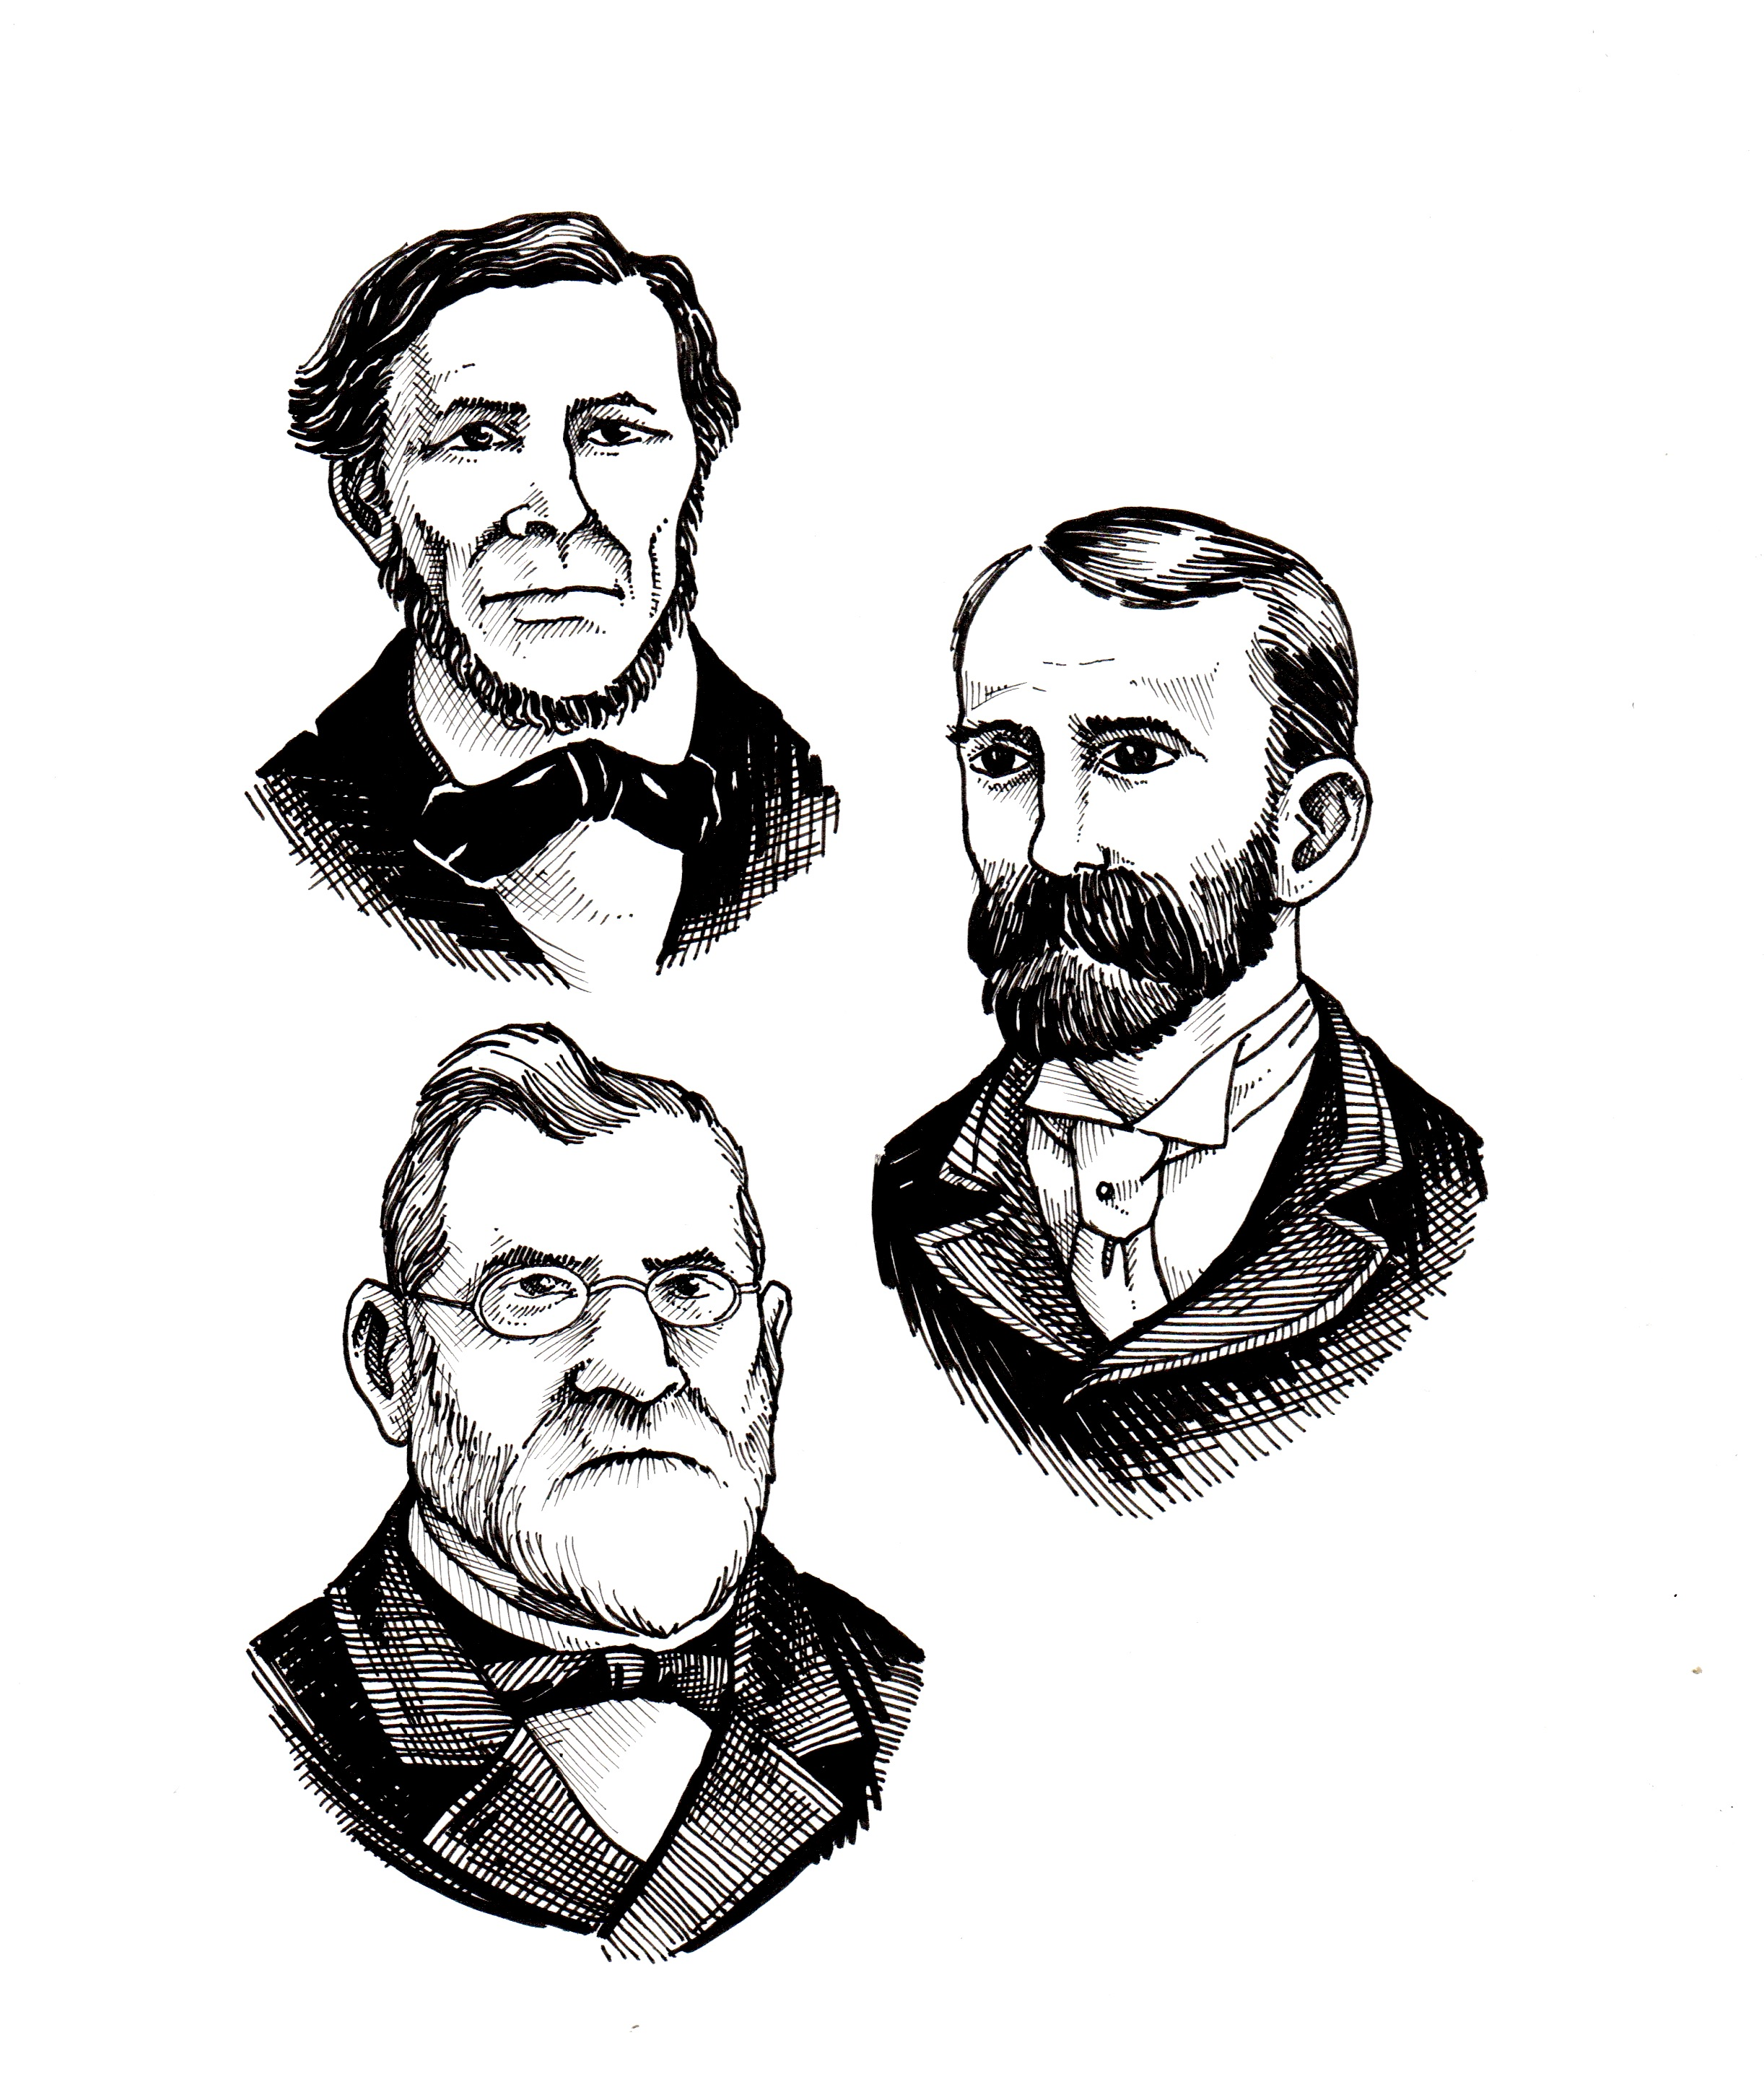
\includegraphics[width=0.6\linewidth,height=\textheight,keepaspectratio]{images/miu3.jpeg}

}

\caption{Theophilus Wylie (top), David Banta (bottom), James Woodburn
(right)}

\end{figure}%

\epigraph{
It will be seen that during the first generation of its history the Indiana University endured a continuous struggle\ldots{}. Yet under its first president, during its first quarter of a century, it continued to do respectable and thorough college work. Under the advancing and more liberal policy of the last twenty years on the part of the State toward her institutions of higher learning, the institution, from being only a training school in the classics and mathematics, is rapidly pushing into the work of the university proper, and offers growing opportunities for advanced and original investigation.}
{---James A. Woodburn, \textit{Higher Education in Indiana}}

Between 1883 and 1885, a series of unforeseen and startling events set
Indiana University on the long road to its current distinction as an
American research university. Shedding its prior identity as an ordinary
classical collegiate institution, the new campus with its fresh
leadership provided energy to pursue ambitious educational goals and
higher aspirations for its academic community. IU got in step with
national trends in higher education, characterized by widespread
university-building fueled by increasing student enrollments, a focus on
research, and renewed commitments to serve society. To make sense of
these changes as well as to further encourage the pursuit of lofty goals
for the institution, the distinct genre of Indiana University history
was invented in the 1880s by a trio of faculty working on individual
projects, with some overlap and collaboration. History-making, through
historical narratives, was a driving force as the university community
confronted its previous sixty-odd years and envisioned a new path
forward.

The quest to assemble a formal university history was made public with
an announcement in the May 1883 issue of the \emph{Indiana Student}.
David D. Banta, president of the IU Board of Trustees, asked for help
from the alumni and former students ``who have any old documents, such
as class programs, catalogues, addresses of professors and presidents,
or other papers pertaining to the University,'' mentioning especially
the 1854 or 1855 catalog of the Athenian Society.\footnote{\citeproc{ref-banta1883a}{\emph{Indiana
  Student} 9, no. 7 (May 1883): 166--67}.} Banta issued this request to
assist longtime professor Theophilus Wylie in preparing the first
``historical catalog'' of the university. Student life at the small
institution located on Second Street and College Avenue centered around
class recitations and the self-governed literary societies, including
the Athenian Society and its chief rival, the Philomathean.

The following month, the 1883 IU commencement featured an alumni reunion
and the award of an honorary LLD (Doctor of Laws degree) to Andrew Wylie
Jr., the eldest son of the first president, Andrew Wylie. The son, a
member of the class of 1832, the third graduating class, had become a
lawyer and was an associate judge of the Supreme Court of the District
of Columbia in Washington, DC, appointed by President Abraham Lincoln.

The alumni society, first constituted in 1854 in the wake of the campus
fire, had been revived a couple of years previously after years of
organizational neglect and recently had made efforts to lobby the
Indiana General Assembly for increased support for the university. Their
efforts paid off in March 1883, when legislation was passed that
established a permanent endowment fund from the state.\footnote{The
  Society of the Alumni was organized in 1854 to provide moral and
  financial support in the wake of the College Building fire. See Janet
  Carter Shirley, \citeproc{ref-shirley2004a}{\emph{The Indiana
  University Alumni Association: One Hundred and Fifty Years,
  1854--2004} (Bloomington: Indiana University Alumni Association,
  2004)}.}

In July 1883, a catastrophic fire struck the deserted campus, burning
the newest of the two main buildings, Science Hall, only ten years old.
Since there were no eyewitnesses and a heavy rainstorm at the time, a
lightning strike was assumed to be the cause. The building was a total
loss, and the thirteen-thousand-volume library, collections of fossils
and of fishes, physical and chemical apparatuses, and faculty books and
papers were among the items destroyed.\footnote{\citeproc{ref-woodburn1940a}{Woodburn,
  \emph{History of Indiana University}, 1940, 332--35}.}

The fire set into motion actions by the IU Board of Trustees that would
have far-reaching effects on the small collegiate institution. By
August, trustees were debating whether to relocate the university. Some
already thought that the ten-acre campus was inadequate, being hemmed in
by the railroad on its western boundary since 1853 with its noise,
vibration, and clutter. The fire became another argument to move.
Bloomington, with its 3,000 citizens, was growing and had ample land for
sale. The trustees looked at eleven parcels and decided to move the
university to the eastern outskirts of the town, to a twenty-acre
woodlot on the Dunn family farm.

\section{From Seminary Square to Dunn's
Woods}\label{from-seminary-square-to-dunns-woods}

Dunn's Woods, purchased by the trustees for \$6,000, became the site of
the new campus. In September, the commissioners of Monroe County made a
\$50,000 donation toward construction costs to rebuild the
university.\footnote{\citeproc{ref-wylie1890a}{Wylie, \emph{Indiana
  University, Its History from 1820, When Founded, to 1890, with
  Biographical Sketches of Its Presidents, Professor and Graduates, and
  a List of Its Students from 1820 to 1887}, 84}.} The next month,
science professor David Starr Jordan, away on a collecting expedition,
wrote to IU president Lemuel Moss: ``I am glad to hear of the general
brightness of the prospects of the institution. The Dunn's Woods project
I do not quite understand, but the location is certainly better among
those great maples. I hope that you will let none be cut down, except
when their removal is absolutely necessary.''\footnote{\citeproc{ref-jordan1883a}{David
  Starr Jordan, {``Letter to Lemuel Moss,''} October 7, 1883.
  IUA/C73/B1/F Jordan, David Starr}.}

The trustees hired Indianapolis architect George W. Bunting to design
three buildings, two of brick and one of wood, and plans were submitted
in November 1883. Ground was broken in April 1884 at the new campus,
hopefully renamed University Park, and construction commenced using
recycled bricks from the burned building. Meanwhile, professors and
students soldiered on at the old campus, the ruins of Science Hall a
daily sight.

Change was not limited to the built environment; it also extended to the
university's leadership. In the first semester of the 1884--85 year, a
group of six students plus the janitor, Thomas ``Uncle Tommy'' Spicer,
drilled a small hole in the floor above one of the rooms in the
surviving university building. There were rumors of an affair between
President Moss, a Baptist minister and a married man, and the young
professor of Greek, Katharine Graydon, a single woman. Through the spy
hole, the students observed the two kissing and caressing and reported
it to the trustees.\footnote{Later,
  \href{http://webapp1.dlib.indiana.edu/archivesphotos/results/item.do?itemId=P0024044&searchId=0&searchResultIndex=1}{a
  picture} was staged with the seven ``Moss Killers,'' displaying a wood
  drill, keyhole saw, and a hatchet on the wall behind.} The trustees,
duty bound to launch their own investigation of this serious violation
of social norms, set a hearing date for November 11. Graydon submitted
her resignation letter on November 5, followed three days later by Moss.
The trustees called off the investigation immediately, likely relieved
that the university would not have to air its dirty laundry in public
after all.\footnote{Minutes of the IU Board of Trustees, November 1884.
  Graydon tried to retract her letter of resignation the following
  month, but the trustees refused to consider it. Indiana University
  Board of Trustees, \citeproc{ref-botm1884a}{{``Minutes of the Board of
  Trustees of Indiana University, 06 November 1884--11 November 1884''}
  (Bloomington: Indiana University Archives \& Indiana University
  Libraries Digital Collections Services, November 7, 1884),
  \url{https://purl.dlib.indiana.edu/iudl/archives/iubot/1884-11-07}}.}
The trustees appointed seasoned professor of languages Elisha Ballantine
as acting president.

The trustee board immediately launched a search for a new president.
Several candidates were considered from a list containing forty-seven
names, but in the end, the trustees chose biology professor David Starr
Jordan, a prominent ichthyologist on the faculty since 1879, as the
seventh president of Indiana University.\footnote{\citeproc{ref-botm1884b}{Indiana
  University Board of Trustees, {``Minutes of the Board of Trustees of
  Indiana University, 16 December 1884--19 December 1884''}
  (Bloomington: Indiana University Archives \& Indiana University
  Libraries Digital Collections Services, December 1884),
  \url{https://purl.dlib.indiana.edu/iudl/archives/iubot/1884-12-16}}.}
Trained at Cornell University and influenced by its progressive
president, Andrew Dickson White, Jordan was a staunch Darwinian and an
avowed proponent of the research ideal. He was a popular professor,
taking students on natural history rambles in the area surrounding
Bloomington and pioneering weeks-long expeditions to Europe, called
``summer tramps,'' to sample aspects of natural as well as cultural
history.

Jordan took office on the first day of January 1885, announcing: ``I
believe our University is the most valuable of Indiana's possessions. It
is not yet a great University, it is not yet a University at all, but it
is the germ of one and its growth is as certain as the progress of the
seasons.''\footnote{\citeproc{ref-jordan1922a}{\emph{Days of a Man,
  Being Memories of a Naturalist, Teacher, and Minor Prophet of
  Democracy}, vol. 1 (Yonkers-on-Hudson, NY: World Book Company, 1922),
  295}.}

The IU trustees, headed by Banta, had faced three major challenges in
the previous eighteen months: the burning of the best building on
campus, the decision for a wholesale removal to a new site, and an
unanticipated change of presidential leadership. Further changes were
afoot in the expansion of the curriculum to embrace scientific fields,
the reorganization of the faculty into departments, and the institution
of the ``major'' course of study for students. As President Jordan
explained, ``The highest function of the real University is that of
instruction by investigation, and a man who cannot and does not
investigate cannot train investigators.''\footnote{Jordan made this
  statement in his 1888 report as a trustee of Cornell University;
  quoted in W. T. Hewett, \citeproc{ref-hewett1905a}{\emph{Cornell
  University: A History}, vol. 1 (New York: University Publishing
  Society, 1905)}, p.~286.}

To some longtime faculty members, the pace of change provoked
apprehension. Theophilus Wylie, granted emeritus status in 1886, wrote
in his diary: ``New arrangements, new studies, new teachers, new modes
of teaching, give me much anxiety.''\footnote{\citeproc{ref-wylie1885a}{{``Diary
  Entry''} (Indiana University Archives, September 6, 1885)}.} Some
others might have shared Wylie's disquiet, but students were voting with
their feet to come to the new University Park, as enrollments surged
after 1885.

To improve faculty quality in the face of limited financial resources,
Jordan began filling vacancies with professors from eastern
institutions, but most ``failed to adapt themselves, appearing to feel
that coming so far West was a form of banishment.'' So, he took a page
from Hoosier agricultural heritage and populated the faculty with
homegrown talent. He started the Specialist's Club for gifted students,
and he promised talented recent IU graduates ``professorships when they
had secured the requisite advanced training in the East or in
Europe.''\footnote{\citeproc{ref-jordan1922a}{\emph{Days of a Man, Being
  Memories of a Naturalist, Teacher, and Minor Prophet of Democracy},
  1:295}.} Among the many alumni he inspired to become Indiana faculty
stalwarts were Joseph Swain, William Lowe Bryan, Carl Eigenmann, James
A. Woodburn, David Mottier, and William Rawles.\footnote{\citeproc{ref-jordan1922a}{Jordan,
  1:295--96}; Cf. \citeproc{ref-capshew2011a}{Capshew, {``Indiana
  University as the {`Mother of College Presidents'}''}}.}

In the fall of 1885, classes opened on the new campus. The three new
buildings---Wylie, Owen, and Maxwell (later renamed
Mitchell)---contained classrooms, laboratories, and offices. The old
College Building at Seminary Square was still being used for the IU
Preparatory Department and large gatherings. Events of the previous two
years ``uprooted the institution, and the new campus opened in 1885
without a sense of history,'' as historian Howard McMains later
noted.\footnote{\citeproc{ref-mcmains2010a}{{``The Indiana Seminary
  Charter of 1820,''} 359}.}

\section{Inventors of IU History}\label{inventors-of-iu-history}

As Indiana University worked through significant changes in the 1880s, a
trio of faculty were working, separately and together, to craft the saga
of the institution. Each brought different talents and angles of vision
to the task of making sense of the recent changes. To be sure, the
university had survived serious threats to its welfare, even its
existence as an institution, almost since the beginning of instruction,
but things were different this time. Nearly every aspect of the
university---physical plant, curriculum, leadership, state
relations---was affected. In the face of a period of major changes,
there was an inevitable distinction to be made between the time leading
up to the period and the time since. In simple terms, there was a clear
``before'' and ``after.'' That distinction, whether explicitly
acknowledged or not, became the main armature around which the trio of
faculty historians shaped their narratives about IU.

The first, in terms of seniority and length of faculty service, was
Theophilus Wylie (1810--95). A younger half-cousin of the first
president, Andrew Wylie, he was hired to teach natural science and
chemistry in 1837. He taught many other subjects over his long teaching
career as well. Wylie also served a variety of administrative posts,
including librarian and president \emph{pro tem} of the small
university. Thus, he was in a good position when the board of trustees
asked him, in 1881, to prepare a historical catalog documenting the
history of IU for its first six decades. He was appointed IU vice
president in 1882 but resigned from this position in June 1884 to free
up more time for historical research and asked Banta for
assistance.\footnote{\citeproc{ref-botm1884c}{Indiana University Board
  of Trustees, {``Minutes of the Board of Trustees of Indiana
  University, 04 June 1884--11 June 1884''} (Bloomington: Indiana
  University Archives \& Indiana University Libraries Digital
  Collections Services, June 7, 1884),
  \url{https://purl.dlib.indiana.edu/iudl/archives/iubot/1884-06-04}};
  cf. \citeproc{ref-myers1951a}{Burton Dorr Myers, \emph{Trustees and
  Officers of Indiana University 1820--1950}, ed. Ivy L. Chamness and
  Burton D. Myers (Bloomington: Indiana University, 1951), 484--85}.}

The second member of the trio was David D. Banta (1833--96), a former
Indiana circuit court judge who became an IU trustee in 1877, serving as
board president from 1882 to 1889. He was appointed dean of the newly
revived law school in 1889, serving until his death in 1896. He received
two degrees from IU: a Bachelor of Science in 1855 and a Bachelor of
Laws in 1857. Banta, a successful lawyer and judge, was a self-trained
historian, completing a history of the Presbyterian Church in Franklin,
Indiana, in 1874. As president of the IU Board of Trustees, he was a key
figure during the momentous transition in the university's campus
location and leadership from 1883 to 1885.

The trio's last member, James Albert Woodburn (1856--1943), represented
yet another, more recent, generation. Son of faculty member James W.
Woodburn (1817--65), he had been baptized at seven months by Theophilus
Wylie at Bloomington's Presbyterian church.\footnote{Theophilus Wylie,
  \citeproc{ref-wylie1857a}{{``Diary Entry''} (Indiana University
  Archives, June 28, 1857)}: ``Baptized James Albert, sone
  {[}\emph{sic}{]} of James \& Martha Woodburn{[}.{]} Weather warm,
  summer like.''} The younger Woodburn had been educated in Bloomington
schools and attended IU, receiving a Bachelor of Arts in 1876 and a
Master of Arts in history in 1885. In 1879, he began teaching in the IU
Preparatory Department and later became a member of President Jordan's
Specialist's Club for future faculty members. Securing a leave of
absence from IU in 1886, Woodburn pursued a doctorate in history from
Johns Hopkins University, studying in the famous seminar guided by
Herbert B. Adams. In his absence, in 1888, he was promoted to associate
professor of history at IU. After writing a dissertation examining the
history of higher education in Indiana, he earned his Doctor of
Philosophy in 1890.

Both Woodburn and Banta were IU alumni, and each became acquainted with
Theophilus Wylie as college students. Starting in 1879, the trio spent
sixteen years on the IU staff together until Wylie's death in 1895,
followed a year later by Banta's passing. All were steeped in the
traditions of the Seminary Square campus, but each had a different
viewpoint based on their personal observations and associations. Wylie
was in the final phase of his long teaching career and now embarking on
a laborious accounting of all the people who had belonged to the
university since 1820---students, faculty, presidents, and trustees.
Banta, as president of the trustee board, played a key role in steering
the university's course in the turbulent mid-1880s. Pressed into service
as the dean of the newly revived law school in 1889, he became a senior
faculty figure too. Woodburn, nearly a half century younger than Wylie,
was just starting his professorial career, albeit with a family
background that had been connected to IU since the late 1830s.

\section{Toward a Historical Catalog}\label{toward-a-historical-catalog}

When he started the historical catalog project in 1881, Wylie thought it
would take him about three years. The intent of the work, according to
the trustees' request, was to showcase the university's contribution to
the state and the nation through the impact of its faculty and alumni.
Taking on what he acknowledged as ``a very big task\ldots if it is done
as it ought to be,'' Wylie sent out multiple rounds of postcards and
letters soliciting information from former faculty and students as he
endeavored to compile exhaustive lists and biographical portraits of
professors, presidents, trustees, and students, both graduates and
nongraduates, since the university's beginning in 1820 as the state's
seminary of learning.

Wylie's painstaking work was frustrated by the loss of university
records and papers by the 1854 campus fire and the more recent burning
of Science Hall in 1883. He sifted through surviving documents, year by
year, for the comings and goings of students and faculty.\footnote{\citeproc{ref-wylie1890a}{Wylie,
  \emph{Indiana University, Its History from 1820, When Founded, to
  1890, with Biographical Sketches of Its Presidents, Professor and
  Graduates, and a List of Its Students from 1820 to 1887}, 3}.} His
wide correspondence with alumni yielded a wealth of materials to replace
missing records and other relevant information.

The lack of sufficient documentation and understanding concerning IU's
past was illustrated by a historical conundrum addressed by the trustee
board in March 1884. In the midst of making plans for the new campus at
University Park (and a few months before the Moss scandal broke), a
point of clarification was raised about another, seemingly minor matter:
``The question of date on the University Seal was brought to the notice
of the Board. After discussing the old date (1830) and the date of the
organization of the Indiana Seminary (1820), the organization of the
Indiana College (1828), and the Indiana University (1838), it was agreed
by general counsel to fix the date of the seal at 1820, the other
devices to remain as in the former seal.''\footnote{\citeproc{ref-botm1884d}{Indiana
  University Board of Trustees, {``Minutes of the Board of Trustees of
  Indiana University, 04 March 1884--25 March 1884''} (Bloomington:
  Indiana University Archives \& Indiana University Libraries Digital
  Collections Services, March 25, 1884),
  \url{https://purl.dlib.indiana.edu/iudl/archives/iubot/1884-03-04}}.}
Without relevant records to disclose the reason why 1830 was on the
seal, the trustees apparently decided it was a simple mistake and
removed the last X from MDCCCXXX. After the trustees changed the seal to
correspond with the founding date of the institution's earliest
progenitor, the Indiana State Seminary, the trustees moved on to more
pressing business.

Trying to piece together IU's history during extensive institutional
change was not easy for Wylie. On the verge of teaching on the new
campus in September 1885, Wylie confessed his anxiety to his daily
diary.\footnote{\citeproc{ref-wylie1885a}{{``Diary Entry,''} September
  6, 1885}.} In 1886, after successfully completing his final year of
teaching in the new surroundings of University Park, Wylie was granted
emeritus status for his forty-seven years of service.\footnote{Wylie
  first came in 1837, then spent two and a half years at Miami
  University in 1852--54, and then returned to IU.} He was a creature of
the old campus, retaining his emotional connection to Seminary Square.
His living situation reinforced those ties. He had been living in Wylie
House, the former home of the first president, for a quarter century and
raised a large family there. Wylie persevered with his research and
extensive correspondence with members of the university clan for several
years after the center of campus life moved to Dunn's Woods. As the
scope and complexity of the historical catalog continued to evolve,
Banta, who had done some research and writing about the university
himself, became both a contributor to the volume and a member of the
trustee committee supervising its production.

\section{Creating a Foundation
Narrative}\label{creating-a-foundation-narrative}

By the mid-1880s, the university had survived for sixty years, with over
1,200 graduates. Stories of the institution's past, leavened with
folklore, had evolved into an informal oral tradition, passed from
generation to generation. A main source of this oral tradition was
physician David H. Maxwell, the first president of the board of
trustees; the oral tradition was further amplified by his son, James
Darwin Maxwell, also a trustee.

From Jefferson County, the senior Maxwell was a delegate at the
convention that wrote Indiana's first state constitution in 1816. That
document mentioned that the state would provide, at some point in the
future, ``a general system of education, ascending in a regular
gradation from township schools to a State university.''\footnote{Wylie,
  \citeproc{ref-wylie1890a}{\emph{Indiana University, Its History from
  1820, When Founded, to 1890, with Biographical Sketches of Its
  Presidents, Professor and Graduates, and a List of Its Students from
  1820 to 1887}}, p.~14. Maxwell was not a member of the education
  subcommittee that wrote that section of the Indiana Constitution.}

Maxwell, with his wife and young son, moved to Monroe County in 1819, a
year after the county was organized at the northern limit of white
settlement. In 1820, the Indiana General Assembly passed an act to
establish a state seminary of learning, to be organized by a board of
trustees. Maxwell was among the original trustees and was elected
president of the six-member board. In 1828, when the state legislature
established Indiana College, new trustees were appointed, including
Maxwell. He continued as board president for the next decade. In 1838,
the Indiana General Assembly passed ``an act to establish a university
in the State of Indiana'' and a reconstituted board of trustees to
oversee it.\footnote{\citeproc{ref-wylie1890a}{Wylie, 21}.} Maxwell was
not among the original members of this twenty-one-person board, although
he was appointed the following year, serving until 1852. He died weeks
before the 1854 fire that destroyed the College Building.

His son, James Maxwell, also a physician, was an IU alumnus and served
the board of trustees as their appointed secretary from 1838 to 1855
before becoming a trustee himself from 1861 to 1892, the year of his
death.\footnote{James Maxwell served as trustee board president from
  1862 to 1865 during the Civil War.}

Both Maxwells, father and son, lived in Bloomington and were familiar
figures in town and on the IU campus at the end of College Avenue. Their
combined service as trustees spanned seventy years, from the very
beginning of the institution in 1820 into the early 1890s. The main
outlines of the oral tradition emphasized the institution's continuity
and created a narrative of linear progress. It ignored the inconsistent
actions of the Indiana General Assembly and elided the real distinctions
between seminary, college, and university in favor of a \emph{post-hoc}
vision of inevitable advancement.

Until his death in 1854, Maxwell was a regular figure on campus. Banta,
who graduated in 1855, ``remembered him with great respect'' and ``must
have listened to Maxwell's version of the foundation narrative many
times.'' His son, James Maxwell, was also a familiar sight until his
death in 1892, and no doubt reiterated his father's story.\footnote{\citeproc{ref-mcmains2010a}{McMains,
  {``The Indiana Seminary Charter of 1820,''} 361}.} Indeed, all members
of the trio who invented IU history had ample occasions to hear the
origin story from a Maxwell---father or son or both.

When Banta, now the revived law school dean, was chosen to present the
inaugural Foundation Day address in 1889, he spoke on the Indiana
Seminary, crystallizing the informal oral tradition informed by Maxwell
into historical doctrine. The story was that David Maxwell, acting as an
unofficial lobbyist to the legislature meeting in Corydon in December
1819, pressed for the location of a seminary of learning in Monroe
County. With the support of Governor Jonathan Jennings, a bill
authorizing the creation of a state seminary was narrowly passed on
January 20, 1820. Banta admitted in his narrative that ``no record, no
tradition even, remains to tell the story of what he did, to secure
legislative action on behalf of a State school.'' Maxwell's subsequent
actions as a trustee over the next thirty years led Banta to declare
that ``he was the Father of the Indiana University.''\footnote{\citeproc{ref-banta1914b}{{``History
  of Indiana University {I},''} 9}.}

For the next five years, Banta gave Foundation Day addresses,
elaborating on the history of the institution to 1850. With this
official imprimatur, the origin story became further solidified as a
linear chronicle of Indiana State Seminary (1820--28), Indiana College
(1828--38), and Indiana University (since 1838).

After a decade of effort, Wylie's historical catalog was finally
published in 1890, under the title \emph{Indiana University, Its History
from 1820, When Founded, to 1890, with Biographical Sketches of Its
Presidents, Professors and Graduates, and a List of Its Students from
1820 to 1887}. It contained an abbreviated chapter from Banta on the
Indiana seminary, as well as a chapter on the university's legislative
history written by Robert S. Robertson, a trustee. The bulk of the book
was filled with biographical sketches of students, professors,
presidents, and trustees with short narrative sections covering the
collegiate department and law school.\footnote{\citeproc{ref-wylie1890a}{Wylie,
  \emph{Indiana University, Its History from 1820, When Founded, to
  1890, with Biographical Sketches of Its Presidents, Professor and
  Graduates, and a List of Its Students from 1820 to 1887}}.}

Meanwhile, James Woodburn was away in Baltimore, on a leave of absence
from IU to work on a Ph.D.~in history. Shortly after Banta delivered his
first Foundation Day address in January 1889, Woodburn wrote to him
about IU history. Banta replied, ``Anything in my paper you find of
service to you in your monograph you are welcome to use.'' Banta talked
about the Hoosier pioneers who ``were much in earnest in their desire
for educational advancement'' but they faced three main obstacles: ``In
the first place the great poverty of the people and in the second the
physical obstacles such as unprecedented sickness prevailing generally
and the difficulties incident to a region so densely wooded as was Ind.;
and in the third place want of models. Every thing {[}\emph{sic}{]} had
to be worked out of the green and it required the labor of 50 years to
get the field ready.''\footnote{\citeproc{ref-banta1889a}{{``Letter to
  James Woodburn''} (Indiana University Archives, February 9, 1889)}.}

Later that year, Woodburn finished his historical monograph,
\emph{Higher Education in Indiana}, and in 1890 received his doctoral
degree. His mentor, Herbert Adams, was editing a series of studies,
Contributions to American Educational History, for publication by the US
Bureau of Education. Woodburn's dissertation found a place in the series
and was published by the bureau in 1891---his first publication with
Ph.D.~appended to his name.\footnote{\citeproc{ref-woodburn1891a}{James
  Albert Woodburn, {``Higher Education in Indiana,''} ed. Herbert B.
  Adams, Bureau of Education, Circular of Information No. 1, 1891:
  Contributions to American Educational History (Washington: Government
  Publishing Office, 1891)}.}

Woodburn hewed to the existing foundation narrative in his two chapters
on the evolution of Indiana University, writing about the historical
progression of seminary, college, and university in an unproblematic
way. The view from the present was reinforced by eight illustrations of
the buildings of the new campus at Dunn's Woods and only one from the
old campus at Seminary Square, still in use for the preparatory
department. He also singled out the contributions of David Maxwell: ``In
the establishment of institutions, it seems that the life and services
of some one man are paramount and essential. In the establishment of the
Indiana Seminary Dr.~David H. Maxwell was the essential
man.''\footnote{\citeproc{ref-woodburn1891a}{Woodburn, 77}. Comma added.}

The lack of institutional records, exacerbated by two great campus
fires, combined with the perceived need to account for the university's
history in the 1880s, led to agreement among the three faculty members
about the foundation narrative. For over a century, subsequent
historians of IU have uncritically echoed that judgment about the
institution's origins and early development.

More recently, contemporary scholars are indebted to historian Howard
McMains's revisionist account of the early history of the institution
that would become Indiana University. He examined the historical
construction that the charter of the Indiana State Seminary was foretold
in the state's constitution, thus ``laying the bottom rail'' for Indiana
University, as every previous IU historian had written. McMains
explained, ``The constitution had not\ldots contemplated the seminary
charter; the seminary charter had not contemplated the university.'' But
David Maxwell connected the two together: ``His narrative inserted the
institution into the very origins of the state and linked constitution,
seminary, and college into a seamless development\ldots{[}and{]} also
made a university in Bloomington seem inevitable.''\footnote{``Laying
  the Bottom Rail'' was the title of chapter 3 in Clark,
  \citeproc{ref-clark1970b}{\emph{Indiana University}, 1970}, p.~25.
  McMains, \citeproc{ref-mcmains2010a}{{``The Indiana Seminary Charter
  of 1820''}}, pp.~378--379.} By carefully reexamining both surviving
documents and the political and social context, his article lends
support to the contention that the foundation narrative created in
1889--91 was not a straightforward piece of historical reporting but an
account shaped first by David Maxwell to lend legitimacy to the notion
that the seminary was the seed of the university and then by subsequent
historians to provide a comforting sense of institutional progress to
the circumstances of their present day.

\section{A Case of Collective
Amnesia}\label{a-case-of-collective-amnesia}

The process of constructing a foundation narrative for the institution
required a selective reading of past evidence. With the destruction of
records and the limits of human memory, the dates of certain key events
were lost to history or misremembered, at least for a time. One example
occurred at the time IU's origin story was being solidified. Recall that
in 1884, the board of trustees, headed by David Banta, believing the
University Seal to be misdated, changed the date on the seal from
MDCCCXXX (1830) to MDCCCXX (1820). They thought it was a simple
misdating of the seminary's founding. Eight years later, Banta, now dean
of the law school, reinforced that decision in his 1892 Foundation Day
address, ``The `Faculty War' of 1832.'' In his introduction, he spoke of
inscriptions as historical evidence:

\begin{quote}
There is one inscription very close to us that falsifies the truth of
history. It is over the east front entrance of this College building. It
states that the Indiana University was founded in 1830, and for the
benefit of those who may not happen to know better, let me say that
there is not a word of truth in that statement. The Indiana Seminary was
chartered on January 20, 1820, the day we commemorate\ldots.I know of no
excuse for the false record inscribed in the stone over the College
door, and I know not whether it was the result of ignorance or of
mistake. There is nothing connected with this institution which was
founded in 1830.\footnote{\citeproc{ref-banta1914a}{{``History of
  Indiana University,''} 1914, 370}; see also
  \citeproc{ref-woodburn1940a}{Woodburn, \emph{History of Indiana
  University}, 1940, 483}, which repeats this interpretation
  uncritically.}
\end{quote}

Banta devised a likely story to support the trustees' 1884
interpretation that it was a simple mistake. Conveniently, it reinforced
the narrative of linear progress from the seminary.

But 1830 did mark a historic date for the small collegiate institution:
it was the first year that Indiana College granted degrees. After ten
years of planning and five years of classes, four students finally
finished the requirements for a baccalaureate degree in 1830. Now the
institution had begun to have success in its raison d'être. In the
eleven years following, another sixty-five students received their
degrees. In total, eight classes (1830--37) were awarded degrees from
Indiana College.\footnote{Degrees awarded from Indiana College,
  1830--37, and Indiana University, 1838--41:

  \begin{itemize}
  \tightlist
  \item
    1830: 4
  \item
    1831: 4
  \item
    1832: 5
  \item
    1833: 3
  \item
    1834: 4
  \item
    1835: 4
  \item
    1836: 8
  \item
    1837: 10
  \item
    1838: 10
  \item
    1839: 7
  \item
    1840: 5
  \item
    1841: 5
  \end{itemize}}

On February 15, 1838, the Indiana General Assembly elevated Indiana
College to Indiana University. Section 4 read: ``The said trustees shall
cause to be made for their use, one common seal, with such devices, and
inscription thereon, as they shall think proper, under and by which all
deeds, diplomas and certificates and acts of the said corporation shall
pass and be authenticated.''\footnote{\citeproc{ref-botm1838a}{Indiana
  University Board of Trustees, {``Minutes of the Board of Trustees of
  Indiana University, 15 February 1838''} (Bloomington: Indiana
  University Archives \& Indiana University Libraries Digital
  Collections Services, February 15, 1838),
  \url{https://purl.dlib.indiana.edu/iudl/archives/iubot/1838-02-15}}.}
Several months later, in September, President Andrew Wylie received the
following instruction from the board of trustees: ``Resolved That Pres't
Wylie be requested to procure a Seal for the University, with such
engravings and devices as he may think appropriate, and also a
{[}printing{]} plate for Diplomas.''\footnote{\citeproc{ref-botm1838b}{Indiana
  University Board of Trustees, {``Minutes of the Board of Trustees of
  Indiana University, 24 September 1838--27 September 1838''}
  (Bloomington: Indiana University Archives \& Indiana University
  Libraries Digital Collections Services, September 27, 1838),
  \url{https://purl.dlib.indiana.edu/iudl/archives/iubot/1838-09-24}}.}
In 1841, the trustee board approved the original university seal, with
the date MDCCCXXX, with no further discussion.\footnote{\citeproc{ref-botm1841a}{Indiana
  University Board of Trustees, {``Minutes of the Board of Trustees of
  Indiana University, 19 July 1841--24 July 1841''} (Bloomington:
  Indiana University Archives \& Indiana University Libraries Digital
  Collections Services, July 21, 1841),
  \url{https://purl.dlib.indiana.edu/iudl/archives/iubot/1841-07-19}}.}
Diplomas were the primary documents affixed with the seal, but it was
also carved on the stone portals of the second College Building in 1855
after the first College Building was destroyed by fire.\footnote{In
  1908, the portals were removed and integrated into the structure of
  the Rose Well House on the Dunn's Woods campus.}

Paying attention to context, there is a good argument that the seal's
original date was no error. The seal had a symbolic function and was
featured on diplomas for certification and validation. In its early
years, the institution was small and precarious. After the 1838 name
change, it was still a small struggling college for many years, but its
aspirations had enlarged as it met with success, year after year, in
slowly increasing the number of its graduates. The 1841 trustees well
knew that the true mark of institutional accomplishment was the
completion of the recurring cycle of higher education---and there had
been one dozen graduating classes at the time the seal was approved.

Four decades later, the context had changed substantially. In the
immediate aftermath of the Science Hall fire that led to the purchase of
Dunn's Woods, the 1884 trustees were newly concerned about institutional
history. Where was the university headed? Where had it been? Stories
about the inevitable advancement of Indiana University from its
precursors, Indiana State Seminary and Indiana College, provided a
comforting narrative of linear progress in the past during a time of an
uncertain present.

Moreover, annual commencements had become an ordinary feature of the
campus calendar, involving dozens of graduates in the 1880s rather than
the handful of the 1830s and 1840s. Interest had moved to the
consideration of the institution's statutory origins---the 1816
congressional land grant and the 1820 legislative act creating a
seminary of learning. But some basic facts about the university's
operation, such as the date of the original University Seal or the date
when classes started, were misremembered, and lost to collective memory
for a time.\footnote{See \citeproc{ref-hackerd2008a}{Jeremy L. Hackerd,
  {``The Complex History of the Date Classes Began at the State Seminary
  of Indiana''} (Indianapolis: Indiana Historical Bureau, June 30,
  2008). background report on the state historical marker ("State
  Seminary of Indiana" marker) for Seminary Square, Bloomington, Indiana
  State Historical Marker Program}.}

\section{Lack of Primary
Documentation}\label{lack-of-primary-documentation}

Determining key facts in IU's chronology has been hampered by a lack of
primary documentation. Many early university records did not survive the
campus fires. A prime example is the confusion about the date classes
began at the state seminary. With primary sources unavailable, some
university histories have claimed that classes began in 1824, and some
have claimed 1825. In 1890, Banta used 1824 in his abbreviated essay
``The Indiana Seminary,'' published in \emph{Indiana University, Its
History from 1820, When Founded, to 1890}, by Theophilus
Wylie.\footnote{\citeproc{ref-wylie1890a}{Wylie, \emph{Indiana
  University, Its History from 1820, When Founded, to 1890, with
  Biographical Sketches of Its Presidents, Professor and Graduates, and
  a List of Its Students from 1820 to 1887}, 38--46}, quote on p.~43.}
When Banta's manuscripts were published in full in the \emph{IU Alumni
Quarterly} in 1914--15, editor Samuel Harding changed a couple of 1825
instances to 1824. In a long footnote, James Woodburn discussed the
ambiguity in the 1940 \emph{History of Indiana University, Volume I:
1820--1902}.\footnote{\citeproc{ref-woodburn1940a}{\emph{History of
  Indiana University}, 1940, 16--17}.} He cites registrar John Cravens,
who told him that ``he had found seemingly good authority for two
dates---1824 and 1825.'' Woodburn agreed with Cravens: ``For the benefit
of future historians, the evidence for both dates is presented
here.''\footnote{\citeproc{ref-woodburn1940a}{16} fn 10.}

Woodburn goes on to discuss various primary sources from outside
university records, concluding with a citation of David Maxwell's 1828
report to the legislature. The document never explicitly dated the
beginning of instruction but can be interpreted as supporting the 1824
date. Woodburn's final comment implied agreement: ``Perhaps on this
evidence we can rest our case.''\footnote{\citeproc{ref-woodburn1940a}{16}
  fn 10.} There things rested for three decades until 1970, when Thomas
Clark published the first volume of \emph{Indiana University: Midwestern
Pioneer}. Based on careful study, including an unearthed newspaper
notice issued by the board of trustees, he determined that the beginning
of classes at the seminary was 1825.\footnote{\citeproc{ref-clark1970b}{\emph{Indiana
  University}, 1970, 30}.}

In 1984, university archivist Dolores Lahrman assigned her assistant,
Bruce Harrah-Conforth, to research the question again. He wrote ``The
Beginning of Classes at Indiana University 1824 or 1825? A Study of
Evidence'' the following year. He argued for 1824, based on counting
backward from David Maxwell's 1828 report to the legislature that stated
the institution had existed for four years. He dismissed the primary
source that Clark cited in support of the 1825 date, claiming that it
merely announced the first day of classes for a particular term, not the
first day of classes ever at the seminary.

Meanwhile, the City of Bloomington planned to renovate Seminary Park and
include important IU dates carved in limestone. In February 1987,
Lahrman wrote to President John Ryan informing him of the city's plan
and lamenting the inconsistent dates for the opening of classes. Since
the publication of Clark's official history, there were some IU offices
using 1824 and some 1825.

Rather than search for additional primary sources and do further
historical research, the board of trustees accepted Harrah-Conforth's
report as definitive and passed a unanimous resolution ``acknowledging
1824 as the year and May 1 as the anniversary date of the beginning of
classes at the State Seminary.''\footnote{\citeproc{ref-botm1987a}{Indiana
  University Board of Trustees, {``Minutes of the Board of Trustees of
  Indiana University, 07 March 1987''} (Bloomington: Indiana University
  Archives \& Indiana University Libraries Digital Collections Services,
  March 7, 1987),
  \url{https://purl.dlib.indiana.edu/iudl/archives/iubot/1987-03-07}}.}
An IU news release was issued immediately: ``The resolution passed today
by the trustees officially resolves that controversy and establishes
1824 as the date to be used in all future university
publications.''\footnote{\citeproc{ref-iu1987a}{Indiana University,
  {``IU Trustees Approve {`Official Year'} of University's First
  Classes''} (Indiana University Archives, March 7, 1987). news
  release}.} It was not clear whether anyone noticed the irony of
overturning a date determined by a reputable historian in the most
recent official IU history in favor of a single, ambiguous document by a
former trustee who was widely known as ``the father of Indiana
University'' in the origin story first set down in the 1880s.

A month later, the eighty-four-year-old university chancellor and former
president Herman Wells sent President Ryan a note, copying archivist
Lahrman: ``I disagreed with Clark's finding when he made it, and so told
him. I am happy, therefore, that further research has revealed that 1824
is the proper date.''\footnote{\citeproc{ref-wells1987a}{Herman B.
  Wells, {``Letter to John Ryan''} (Indiana University Archives, April
  7, 1987)}.} Lahrman responded to Wells with thanks, saying ``it means
a great deal to us to know that you have been for a long time in
agreement. I was apprehensive about undertaking the research, since I
love and respect Dr.~Clark and hate to risk offending him, but it seemed
that we had to try to determine the facts.''\footnote{\citeproc{ref-lahrman1987a}{\emph{The
  History of Mitchell Hall, 1885--1986} (Bloomington: Indiana University
  Archives, 1987)}.} In his reply, Wells congratulated Harrah-Conforth
on his research and Lahrman for initiating action.\footnote{\citeproc{ref-wells1987b}{{``Letter
  to Dolores Lahrman''} (Indiana University Archives, May 13, 1987)}.}

In 2008, Indiana Historical Bureau researcher Jeremy Hackerd made
another run at the vexed issues of dating the beginning of classes. In
charge of the Indiana Historical Bureau Historical Marker Program,
Hackerd exercised due diligence when the City of Bloomington and Indiana
University proposed a state historical marker to commemorate the site of
the Indiana State Seminary. He carefully studied the historiography of
the issue, reexamined old evidence, gathered new information, and
produced an authoritative study. Hackerd concluded:

\begin{quote}
Determining the beginning date for classes at the State Seminary of
Indiana has challenged historians for decades. The use of newly located
primary sources and a reevaluation of interpretations of early standard
sources have resulted in the need to correct the official Indiana
University timeline. Study of the biography of Baynard Rush Hall---the
first teacher, newspaper notices issued by the State Seminary's Board of
Trustees, and Presbyterian church records substantiate April 4, 1825, as
the date classes began at the State Seminary of Indiana in
Bloomington.\footnote{\citeproc{ref-hackerd2008a}{Hackerd, {``The
  Complex History of the Date Classes Began at the State Seminary of
  Indiana.''} background report on the state historical marker ("State
  Seminary of Indiana" marker) for Seminary Square, Bloomington, Indiana
  State Historical Marker Program}.}
\end{quote}

Thus, the mystery that dates to the early history of the institution
found a satisfactory resolution. Ironically, the 1880s marked the
invention of IU history as a literary genre and the creation of
difficult problems with the university's chronology.

\section{Suppression of Historical
Evidence}\label{suppression-of-historical-evidence}

The two examples cited above were unintentional errors exacerbated by
scarce records and faulty memories. Another, more serious case of
distorting the university's history involved David Banta suppressing a
key fact as he recounted the story of the ``faculty war'' of 1832, as
presented in his 1892 Foundation Day address.\footnote{\citeproc{ref-banta1914a}{Banta,
  {``History of Indiana University,''} 1914}.} As mentioned in
Chapter~\ref{sec-two}, the conflict between Andrew Wylie and Baynard R.
Hall began with an anonymous letter left for Hall at the end of the
1830--31 school year. The note eventually led to Hall's resignation. In
the spring of 1832, Professor Harney began having public conflicts with
President Wylie, which led to his dismissal by the trustee board in the
fall. Thus, at the close of Indiana College's seventh year, the original
faculty were gone, and the president and trustees had to recruit new
teaching staff.

Banta learned the identity of the author of the anonymous note when he
received a letter from Andrew Wylie Jr.~in 1882 admitting authorship but
chose to not reveal it in his Foundation Day address a decade later.
Banta never revealed his reasons for suppressing Andrew Wylie Jr.'s name
from his account of the faculty war, but one can surmise some
possibilities. To begin with, both men were judges, with the expectation
that their actions should exhibit probity, restraint, and wisdom. What
would be gained by exposing a major institutional scandal that occurred
sixty years earlier? Better to keep the secret within a small group of
elder figures, perhaps.

The 1882 letter from Wylie to Banta was in the university archives for
over a century, but the secret it contained was not revealed publicly
until a biography of IU's first professor, \emph{Baynard Rush Hall: His
Story}, was published in 2009 by Dixie Kline Richardson.\footnote{For a
  brief account of the secret, see also
  \citeproc{ref-capshew2018a}{James H. Capshew, {``New Light on an Old
  Story: The Secret of the Faculty War,''} \emph{200: The Bicentennial
  Magazine} 1, no. 1 (2018): 6--8}.} Future historians of IU will need
to take account of the fact that a student---the president's son, no
less---started a process that led to the separation of the original
teaching staff from the institution. The episode should be renamed the
``war against the faculty'' rather than the ``faculty war'' possibly.
Regardless, conflict between the administrative staff and instructional
personnel were present from the start.

\section{A Variation on the Theme}\label{a-variation-on-the-theme}

After the various efforts by Wylie, Banta, and Woodburn to construct a
common foundation narrative for the university, a dozen years later
another approach to IU history was tried. After rejecting an invitation
to prepare an exhibit on Indiana University for the 1904 Louisiana
Purchase Exposition in St.~Louis, President William Bryan explained:
``It was determined to prepare a book which should set forth in
permanent form, for those interested, the salient features of the
history and current status of the University. Out of this determination
arose the present volume.''\footnote{\citeproc{ref-harding1904a}{Harding,
  \emph{Indiana University, 1820--1904}, vii}.} The book functioned
along the line of a university viewbook, providing information for the
interested public.

Edited by Samuel B. Harding, professor of European history, the book had
three parts. The first, authored by William Rawles, professor of
economic and social science, was a concise ``Historical Sketch,'' laying
out IU's legislative history and organizational evolution. The works of
the faculty trio were cited at least once, with Woodburn being quoted
several times. The second part was a close study of the ``Development of
the Course of Instruction'' by Lewis Carson, assistant professor of
philosophy. Based on surviving IU catalogs, his text documented the
expansion of the curriculum from ancient classics to modern languages
and the sciences. The final part was a cumulative bibliography of
publications authored by present faculty members, past faculty members,
alumni, and students. Librarian William A. Alexander supervised its
compilation. Both Rawles and Carson eschewed promotional language and
provided sober assessments of their respective subjects. Following the
scholarly model pursued by Woodburn in his earlier study of IU history,
their writing contrasted with Wylie's focus on the academic community or
Banta's storytelling style.

The hybrid volume ritually invoked the past as a prologue to the
university's current aspirations. The number of pages for each section
reveals something about the institution's self-presentation. The first,
containing a brief overview of its development for the last century, was
32 pages (9 percent). The second section, dealing with curriculum, was
160 pages (46 percent), with three-quarters of that (35 percent of the
book) about ``departments as now constituted.'' The final part,
consisting of a bibliography of publications, was 153 pages (44
percent), subdivided into current faculty (28 pages), former faculty (26
pages), and alumni (98 pages). Curriculum and instruction, departmental
organization and facilities, and intellectual production through
scholarship are the key themes of the volume as the university presented
itself to the wider world. History was a relatively minor theme used to
understand the contemporary scene and to implicitly support the
university's aspirations for the future.

\section{Perseveration: The Ritual Use of
History}\label{perseveration-the-ritual-use-of-history}

In 1914, when the first issue of the \emph{Indiana University Alumni
Quarterly} came out, Woodburn---remembering that the historical
addresses of the late law school dean Banta had never been published in
their entirety---arranged with the editor of the new periodical, fellow
history professor Samuel Harding, to have them appear. Banta's
examination of ``The Indiana Seminary'' appeared on page one, signaling
the journal's intent to cover all aspects of alumni experience, past and
present. That 1889 address, given at the first Foundation Day, had first
been published in Wylie's historical catalog in 1890. The following five
issues of the \emph{Alumni Quarterly} published Banta's subsequent
addresses from 1890 to 1894, each for the first time, in a ``History of
Indiana University'' series.\footnote{\citeproc{ref-banta1914b}{Banta,
  {``History of Indiana University {I}''}};
  \citeproc{ref-banta1914c}{Banta, {``History of Indiana University,''}
  1914}; \citeproc{ref-banta1914d}{Banta, {``History of Indiana
  University,''} 1914}; \citeproc{ref-banta1914a}{Banta, {``History of
  Indiana University,''} 1914}; \citeproc{ref-banta1915a}{Banta,
  {``History of Indiana University,''} 1915};
  \citeproc{ref-banta1915b}{Banta, {``History of Indiana University,''}
  1915}.} Later in 1914, Ivy Chamness began working as assistant editor
of university publications and was soon drawn into editing the
\emph{Alumni Quarterly} as well, succeeding Harding.\footnote{See
  Chapter~\ref{sec-eight}.}

Between 1915 and 1917, Woodburn took up where Banta's narrative ended
and published a series of eight articles in the \emph{Alumni Quarterly}.
Under the general title ``Sketches from the University's History,'' he
covered the 1850s at IU in detail. Consequential events included the
employment of Professor Daniel Read, the death of President Andrew
Wylie, and the 1854 campus fire. He included information about student
life, the trustees, and the faculty and curriculum.\footnote{\citeproc{ref-woodburn1915a}{James
  A. Woodburn, {``{Sketches from the University's History I: College Men
  and College Life about 1850},''} \emph{Indiana University Alumni
  Quarterly} 2 (1915): 249--69}; \citeproc{ref-woodburn1915b}{James A.
  Woodburn, {``{Sketches from the University's History II: College Men
  and College Life About 1850 (Continued)},''} \emph{Indiana University
  Alumni Quarterly} 2 (1915): 409--27};
  \citeproc{ref-woodburn1916b}{James A. Woodburn, {``{Sketches from the
  University's History III: Faculty and Curriculum about 1850},''}
  \emph{Indiana University Alumni Quarterly} 3 (1916): 20--37};
  \citeproc{ref-woodburn1916c}{James A. Woodburn, {``{Sketches from the
  University's History IV: Daniel Read, Professor of Ancient Languages,
  1843--1856},''} \emph{Indiana University Alumni Quarterly} 3 (1916):
  127--48}; \citeproc{ref-woodburn1916d}{James A. Woodburn, {``{Sketches
  from the University's History V: Death of President Wylie: A Year of
  President Ryors and Election of Dr. Daily: Death and Services of Dr.
  David H. Maxwell},''} \emph{Indiana University Alumni Quarterly} 3
  (1916): 347--59}; \citeproc{ref-woodburn1916e}{James A. Woodburn,
  {``{Sketches from the University's History VI: The Vincennes Suit and
  the Fire},''} \emph{Indiana University Alumni Quarterly} 3 (1916):
  489--500}; \citeproc{ref-woodburn1917a}{James A. Woodburn,
  {``{Sketches from the University's History VII: Dark Days after the
  Fire: Courage in Adversity},''} \emph{Indiana University Alumni
  Quarterly} 4 (1917): 1--11}; \citeproc{ref-woodburn1917b}{James A.
  Woodburn, {``{Sketches from the University's History VIII: The Board
  of Trustees Sixty Years Ago; Student Reminiscences},''} \emph{Indiana
  University Alumni Quarterly} 4 (1917): 117--28}.}

In 1921, Chamness edited \emph{Indiana University, 1820--1920:
Centennial Memorial Volume}.\footnote{\citeproc{ref-chamness1921a}{Ivy
  L. Chamness, ed., \emph{Indiana University, 1820--1920: Centennial
  Memorial Volume} (Bloomington: Indiana University, 1921)}.} The first
one hundred pages collected all of Banta's articles published in the
\emph{Alumni Quarterly} and republished them as ``History of Indiana
University,'' with the article titles serving as chapter headings. Part
II included the addresses delivered at the Centennial Educational
Conference held at IU in May 1920, under the title ``The American
University: Today and Tomorrow.'' The last part republished a lengthy
account of the Centennial Commencement, written by Chamness for the July
1920 \emph{Alumni Quarterly}.

In 1940, Woodburn finally published History of \emph{Indiana University,
Volume I: 1820--1902}, when he was eighty-four years old.\footnote{\citeproc{ref-woodburn1940a}{Woodburn,
  \emph{History of Indiana University}, 1940}.} The book was divided
into two parts. The first six chapters were authored by Banta and
reprinted, for the third time, the material published in 1914--15 and
republished in 1921. The second part was authored by Woodburn and
contained sixteen chapters, half reprinted from the 1915--17
\emph{Alumni Quarterly} series and half new material. At the end,
addenda were added that contained a miscellany of archival
correspondence and notes that only became known when the manuscript was
in page proofs.

Banta, who died in 1896, was the chief beneficiary of the emerging
practice of perseveration in IU history publishing. He was the first out
of the gate among the trio who invented IU history, delivering an oral
address on the Indiana State Seminary of learning in 1889 at the first
Foundation Day. His subsequent addresses were published many years after
his death, in the first issues of the \emph{Alumni Quarterly} in
1914--15. Then the six articles became part of the 1921 \emph{Centennial
Memorial Volume}. They were reprinted yet again in 1940 as the opening
chapters of Woodburn's \emph{History of Indiana University} volume.
Banta's name has become indelibly associated with IU history.

This insistent repetition might have been justified because each new
student generation should have an opportunity to become acquainted with
the institution's history, but that argument was never made explicitly.
Closer to the truth was the implicit assumption that Banta's narrative
would function as the foundation story, and there was no need for
further work on the early history of the university. In fact, many
people were interested in the university's story, but few had the
interest and skill to write institutional history. Perseveration of
Banta's account through repeated republication was sustained for fifty
years, from 1890 to 1940, a period of tremendous growth and change in
the university. The impulse that animated Banta, Wylie, and Woodburn to
invent IU history in the 1880s had faded, replaced by the ritual
invocation of Banta's stories of the early institution, including the
creation of the state seminary, the coming of President Andrew Wylie,
and the conflict that led to the departure of the original professor,
Baynard Rush Hall.

\section{Postwar Developments}\label{postwar-developments}

In office since 1937, President Herman Wells had a deep appreciation for
the past, filtered through his overriding concern for the improvement of
the university. He inherited two institutional history projects that
began under the previous administration of President Bryan. One was
Woodburn's \emph{History of Indiana University} project, finished in
1940. The other was a project that resulted in a biographical directory,
\emph{Trustees and Officers of Indiana University, 1820--1950},
published in 1951.

In the early 1940s, the Wells administration authorized research for a
second volume of \emph{History of Indiana University}, to cover the
thirty-five-year administration of President William Lowe Bryan from
1902 to 1937. Bryan, still very much alive, was pleased that the author
was Burton Myers, the emeritus dean of the Bloomington medical school
and a valued colleague. Myers was also tasked with bringing the
long-delayed trustees book project to completion.

Spending the better part of a decade researching and writing until his
death in 1951, Myers hewed close to the institutional records of the IU
trustees and the president's office. The result was a dry official
chronicle more than an interpretive narrative. In 1952, \emph{History of
Indiana University, Volume II: 1902--1937, The Bryan Administration} was
published. The massive volume also contained information reaching back
to IU's beginning in the nineteenth century. Whatever its literary
deficiencies, the book remained an invaluable reference source and a
permanent contribution to IU's historiography.\footnote{See
  Chapter~\ref{sec-eight}.}

Through the 1950s and 1960s, Indiana University experienced great
institutional growth in students and faculty, proliferation in academic
programs and facilities, and a remarkable rise in national standing
among research universities. After twenty-five years, the Wells
administration ended in 1962, and the trustees bucked a
seventy-five-year-old tradition of hiring from the inside and selected
Elvis J. Stahr, a former secretary of the army, as president.
Maintaining the university's trajectory set by Bryan and Wells, Stahr
oversaw the continued expansion of IU's educational footprint around the
state as well as gains in faculty research productivity and creative
scholarship. As the university's 150th anniversary approached in 1970,
Stahr appointed Thomas D. Clark, University of Kentucky history
professor (and one of Stahr's former teachers), as visiting professor in
1967 to prepare a new narrative history of Indiana University.

Clark, an experienced regional historian, took on this task with gusto,
examining voluminous primary sources, reading the existing
historiography, and conducting numerous oral history interviews. Not
since Woodburn's 1891 dissertation research had a professional historian
critically explored IU's past---and there was a lot of material after
150 years. The most recent history volume---Myers's (1952)---ended its
coverage in 1937, prior to the Second World War and the tremendous
postwar expansion.

Eventually Clark's project expanded to three volumes of narrative
history and a sourcebook of documents. The first volume of \emph{Indiana
University: Midwestern Pioneer}, published during the IU
sesquicentennial year, was the first retelling of the early history
since Banta. The second volume, published in 1974, focused on the long
presidency of Bryan and his consequential administration. The final
volume came out in 1977, taking the story of IU from 1937 to 1968,
covering the presidential administrations of Wells and Stahr. The volume
garnered excellent reviews, both from the local press and from history
of education scholars.\footnote{Volume I reviews: Maynard Brichford,
  \citeproc{ref-brichford1971a}{\emph{Journal of the Illinois State
  Historical Society (1908--1984)} 64, no. 3 (1971): 355--56,
  \url{http://www.jstor.org/stable/40190803}}; Daniel W. Hollis,
  \citeproc{ref-hollis1971a}{\emph{The Journal of American History} 58,
  no. 1 (1971): 201--2, \url{https://doi.org/10.2307/1890153}}; James
  Nolan, \citeproc{ref-nolan1971a}{{``Indiana University History,''}
  \emph{Courier-Journal}, January 17, 1971}; Winton U. Solberg,
  \citeproc{ref-solberg1971a}{\emph{Indiana Magazine of History} 67, no.
  3 (1971): 268--69, \url{http://www.jstor.org/stable/27789750}}. Volume
  II reviews: J. David Hoeveler, \citeproc{ref-hoeveler1974a}{{``Higher
  Education in the Midwest: Community and Culture {[}Reviewed Volumes
  One and Two{]},''} \emph{History of Education Quarterly} 14, no. 3
  (1974): 391--402, \url{https://doi.org/10.2307/367940}}; Maynard
  Brichford, \citeproc{ref-brichford1975a}{\emph{Journal of the Illinois
  State Historical Society (1908--1984)} 68, no. 3 (1975): 297--99,
  \url{http://www.jstor.org/stable/40191173}}; Merle Curti,
  \citeproc{ref-curti1975a}{\emph{The American Historical Review} 80,
  no. 3 (1975): 518--19, \url{https://doi.org/10.2307/1850710}};
  Patricia Albjerg Graham, \citeproc{ref-graham1974a}{\emph{Indiana
  Magazine of History} 70, no. 2 (1974): 180--82,
  \url{http://www.jstor.org/stable/27789965}}; Daniel W. Hollis,
  \citeproc{ref-hollis1974a}{\emph{The Journal of American History} 61,
  no. 2 (1974): 515--16, \url{https://doi.org/10.2307/1904023}}; John Ed
  Pearce, \citeproc{ref-pearce1973a}{{``The Middle Years of Indiana
  University: A Review,''} \emph{Courier-Journal}, November 18, 1973}.
  Volume III reviews: Merle Curti, \citeproc{ref-curti1978a}{\emph{The
  American Historical Review} 83, no. 4 (1978): 1101,
  \url{https://doi.org/10.2307/1867836}}; Daniel W. Hollis,
  \citeproc{ref-hollis1978a}{\emph{The Journal of American History} 65,
  no. 3 (1978): 836--37, \url{https://doi.org/10.2307/1901512}}; William
  C. Ringenberg, \citeproc{ref-ringenberg1978a}{\emph{History: Reviews
  of New Books} 6 (1978): 148}; Francis P. Weisenburger,
  \citeproc{ref-weisenburger1978a}{\emph{Indiana Magazine of History}
  74, no. 4 (1978): 367--68,
  \url{http://www.jstor.org/stable/27790338}}. Volume IV reviews: George
  W. Knepper, \citeproc{ref-knepper1979a}{\emph{Indiana Magazine of
  History} 75, no. 1 (1979): 95--96,
  \url{http://www.jstor.org/stable/27790359}}.}

The Clark volumes recast the history of Indiana University in a long
narrative arc of 150 years. For the most part, it followed the
foundation story first circulated in the 1880s when institutional
history was mobilized as a university asset, adding a few details but
not challenging the existing framework. Clark was kind to his
predecessors. A key strength of Clark's work was linking the deep and
the more recent past into a single whole, although few readers had the
stamina to read 1,500 pages over three volumes. Symbolically, the
publication represented a turning point, when IU history, written by a
professional historian recruited from beyond the institution, made its
scholarly debut. It also inspired new work and gave it a richer context.
To cite but one example: In 1980, Herman Wells published an
autobiography, \emph{Being Lucky: Reflections and
Reminiscences}.\footnote{\citeproc{ref-wells1980a}{Herman B Wells,
  \emph{Being Lucky: Reflections and Reminiscences} (Bloomington:
  Indiana University Press, 1980)}.} The book ``was, in equal parts, an
engaging autobiography, a manual of higher education management, and an
artful spoof of his stellar career.''\footnote{\citeproc{ref-capshew2012a}{Capshew,
  \emph{Herman {B} Wells}, 332}.} Readers of both volumes can get a
considered view of how Wells transformed the university by perusing
Clark's history, and some flavor of Wells charm and personality that
drove his relentless quest for educational improvement through his
memoirs. Not since David Starr Jordan published \emph{Days of a Man:
Being Memories of a Naturalist, Teacher, and a Minor Prophet of
Democracy} in 1922 had a former IU president engaged
autobiographically.\footnote{\citeproc{ref-jordan1922a}{Jordan,
  \emph{Days of a Man, Being Memories of a Naturalist, Teacher, and
  Minor Prophet of Democracy}}.}

The Clark volumes remain an impressive scholarly monument as well as an
inviting target for revisionist accounts. In the eighty years between
the invention of IU history as a literary genre and the publication of
\emph{Indiana University: Midwestern Pioneer}, accounts of IU's past
have played various roles for the institution and have contributed to
the university's identity and integrity. Since the 1970s, a
comprehensive IU history has not been attempted, much less written.
Perhaps two centuries are too long to cover in sufficient detail or the
currents of fashion for microhistory run too swiftly. One can count on,
however, institutional history playing a key role in the university's
public persona and contributing to the self-understanding of its diverse
community.

\bookmarksetup{startatroot}

\chapter*{Part Two: The Campus at Dunn's Woods}\label{sec-parttwo}
\addcontentsline{toc}{chapter}{Part Two: The Campus at Dunn's Woods}

\markboth{Part Two: The Campus at Dunn's Woods}{Part Two: The Campus at
Dunn's Woods}

\epigraph{
Consult the genius of the place in all.}  
{
\parbox{.75\textwidth}{\raggedleft---Alexander Pope, \textit{Epistles to Several Persons}, "Epistle IV: To Richard Boyle, Earl of Burlington"}}

\begin{figure}[H]

{\centering \pandocbounded{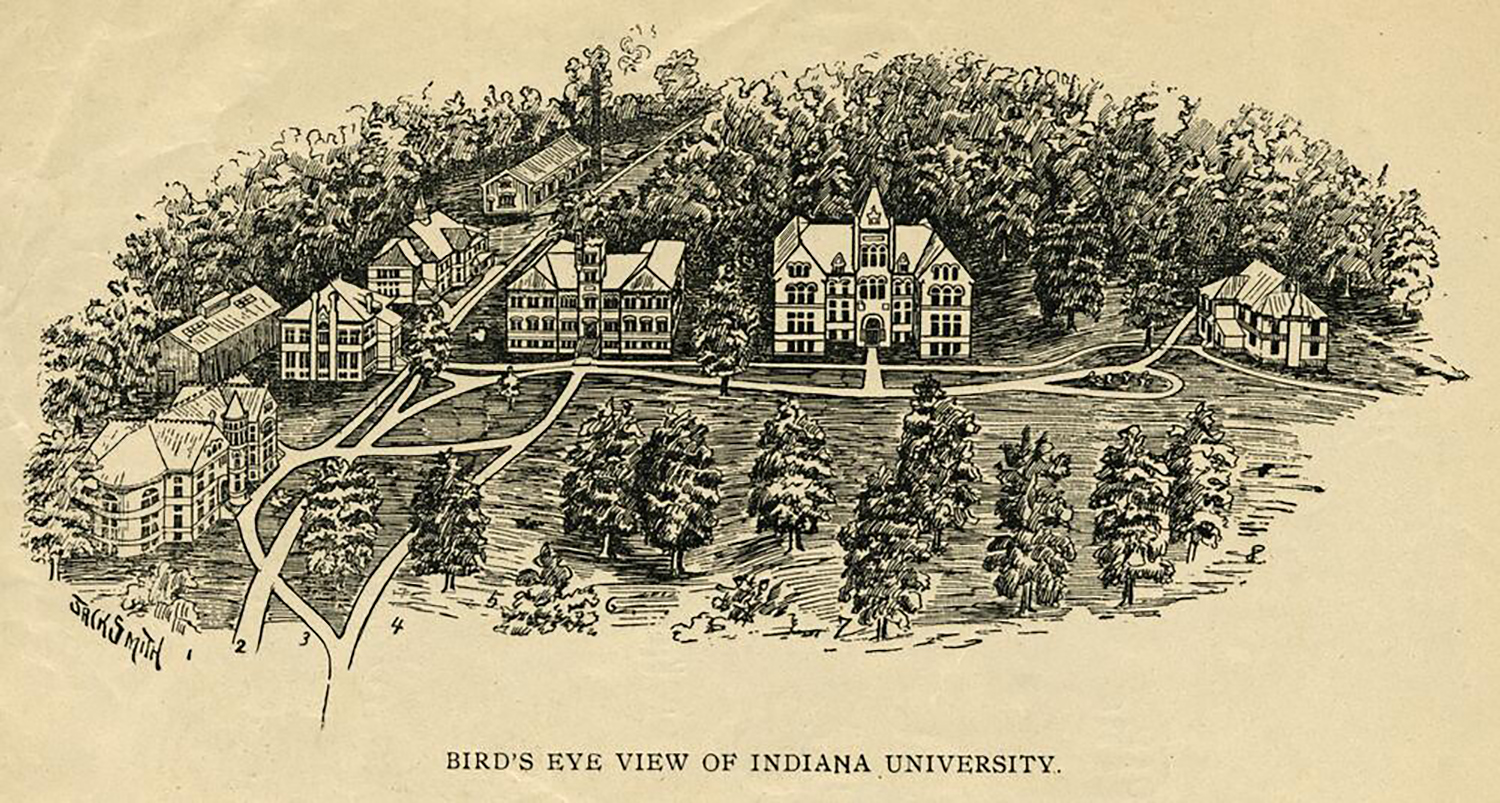
\includegraphics[keepaspectratio]{images/birdseye.jpg}}

}

\caption[A Bird's Eye View of the Campus in 1897]{A bird's eye view of
the campus in 1897, a dozen years after the move to Dunn's Woods. From
left to right, Maxwell Hall, Carpenter Shop (demolished), Owen Hall,
Assembly Hall (demolished), Power Plant (demolished), Wylie Hall,
Kirkwood Hall, Mitchell Hall (demolished). \textbf{© Jack H. Smith.
Image from the
\href{https://libraries.indiana.edu/university-archives}{IU Archives}.}}

\end{figure}%

\bookmarksetup{startatroot}

\chapter{Establishing University Park}\label{sec-four}

\begin{figure}[H]

{\centering 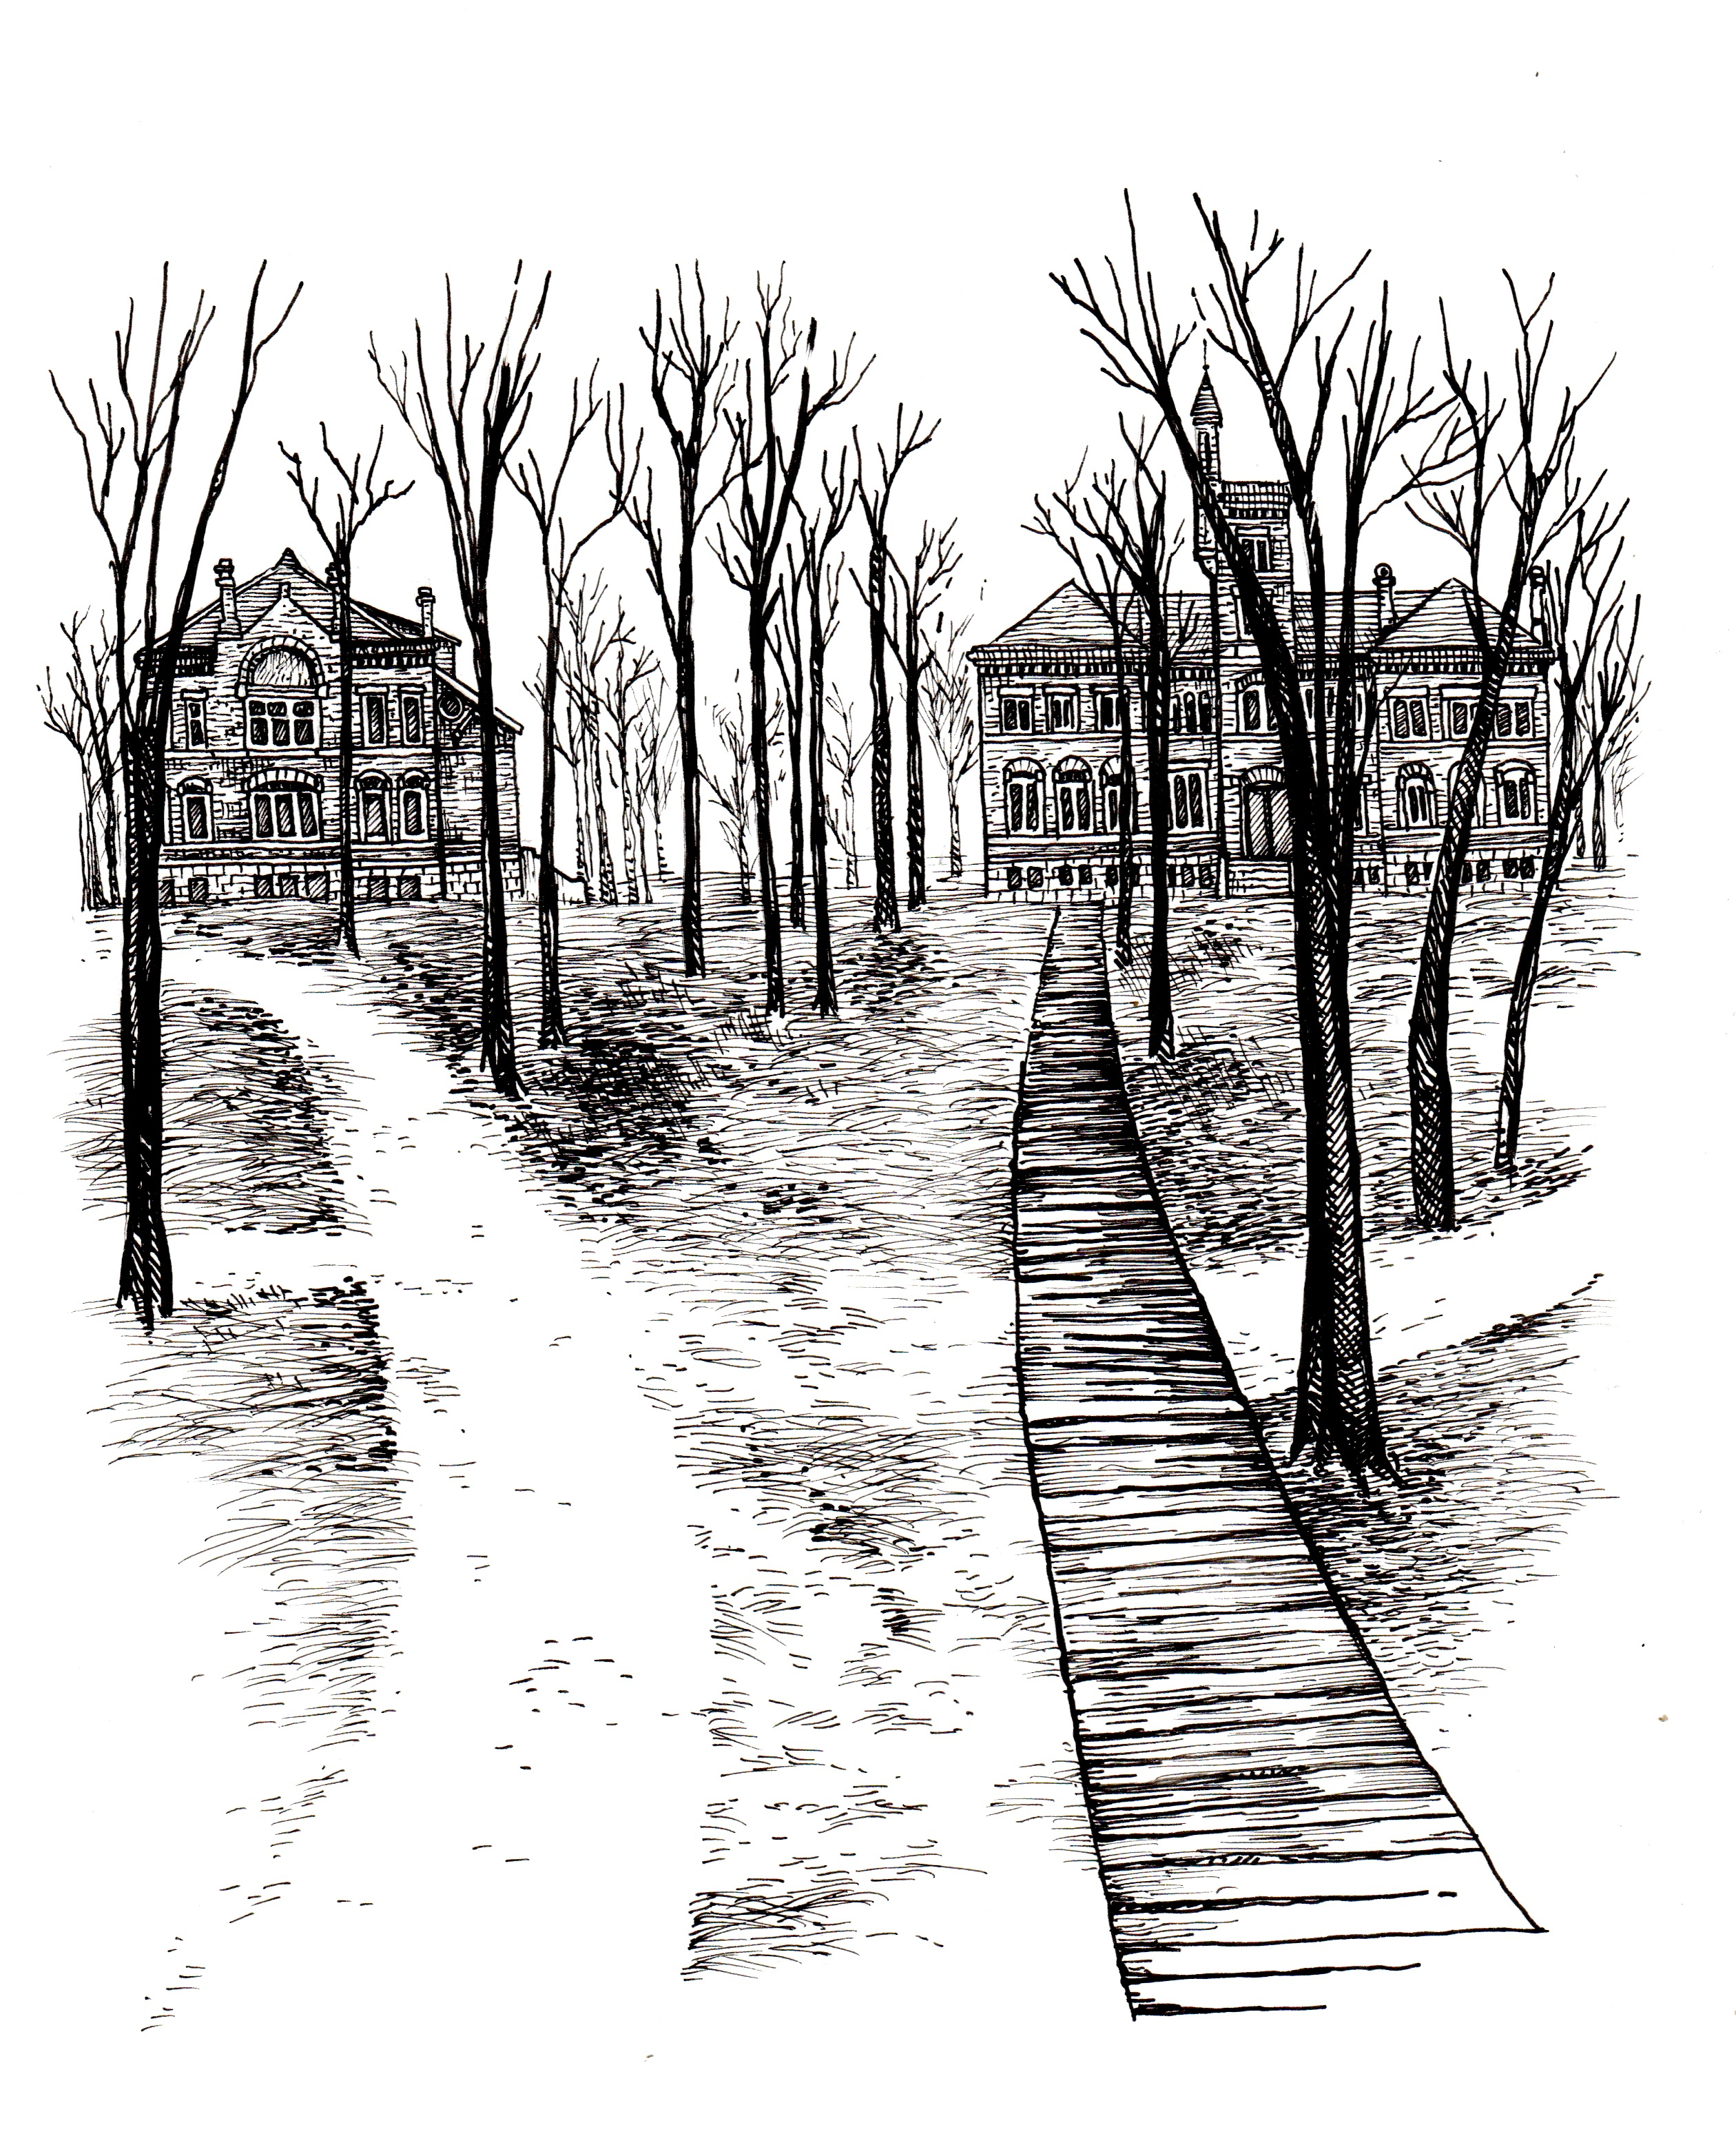
\includegraphics[width=0.6\linewidth,height=\textheight,keepaspectratio]{images/miu4.jpeg}

}

\caption{Owen Hall (left), Wylie Hall (right)}

\end{figure}%

\epigraph{
Places are fusions of human and natural order and are the significant centres of our immediate experiences of the world. They are defined less by unique locations, landscape, and communities than by the focusing of experiences and intentions onto particular settings. Places are not abstractions or concepts, but are directly experienced phenomena of the lived-world and hence are full with meanings, with real objects, and with ongoing activities. They are important sources of individual and communal identity, and are often profound centres of human existence to which people have deep emotional and psychological ties. 
}
{---Edward Relph, \textit{Place and Placelessness}}

By the 1880s, Indiana University had occupied the Seminary Square campus
for nearly sixty years. Carved out of the forest that was Bloomington in
the 1820s, the campus had accommodated a succession of buildings that
served the academic needs of the tiny collegiate institution. The ruins
of Science Hall, destroyed in the 1883 fire, lay next to the College
Building, itself rebuilt in 1855 after an earlier fire. The site had had
hard usage and ``no attention was given to beautifying the campus,'' but
some trees and shrubs had sprung up on their own after the initial
clearing.\footnote{\citeproc{ref-hight1937a}{Kate M. Hight,
  {``Reminiscences,''} \emph{Indiana University Alumni Quarterly} 24,
  no. 4 (1937): 455--60}, quote on 455.}

The IU Board of Trustees was pleased to be getting away from the dirty
clatter of the railroad abutting the campus, away from the industrial
machine and back into the peaceful quiet of the woods. Hoosier attitudes
had changed since the Seminary Square campus was cleared of trees in
frontier Bloomington. Six decades of increasing use of Indiana's forests
led to a growing realization that they were not an inexhaustible natural
resource, and they deserved conservation for the future. In fact, one of
Bloomington's largest employers was the Showers Brothers Furniture
Company, which made wooden bedsteads and other furniture.\footnote{\citeproc{ref-krause2012a}{Carrol
  Krause, \emph{Showers Brothers Furniture Company: The Shared Fortunes
  of a Family, a City, and a University} (Bloomington: Indiana
  University Press, 2012)}.} Overall, forests provided essential
materials for shelter, fuel, and food, and their magnificent forms
dwarfed any manmade structures until the mid-nineteenth century.

The contrast between Dunn's Woods and the original site was stark, and
the move was accompanied by a new appreciation of landscape beauty.
Although wood still provided many of the raw materials for daily life,
no longer was the forest regarded as an obstacle to civilizing forces,
symbolized by a clearing in the wilderness. In a time of widespread
deforestation in the state, now the presence of trees was seen as a
welcome amenity, a moral counterweight to industrial society, where one
could regain a measure of peace and equilibrium by contact with nature.
The university's recent purchase was not virgin forest by any stretch,
but the unimproved farm woodlot did have mature trees that prompted an
aspirational designation as ``University Park'' by the trustees in June
1884.\footnote{\href{https://purl.dlib.indiana.edu/iudl/archives/iubot/1884-06-04}{The
  designation of ``University Park'' died out by 1890.}}

The ideas of Frederick Law Olmsted, landscape designer of Central Park
in New York City, were spreading around the nation, including to
universities and colleges. It was his belief ``that the location and
design of the campus played an essential role in the students'
educational experience'' of equal importance with the academic
curriculum: ``The properly designed campus was part of the civilizing
mission of the college or university, educating the taste and
sensibilities of students.''\footnote{\citeproc{ref-schuyler1997a}{David
  Schuyler, {``Frederick Law Olmsted and the Origins of Modern Campus
  Design,''} \emph{Planning for Higher Education} 25, no. 2
  (1996--1997): 1--10}, quote on p.~10.}

The new site contained twenty acres of a gently sloping hill, generally
oriented west toward the town, with a small brook. Before the university
acquired the land, it was used by local townspeople ``chiefly for the
practice of outdoor speeches, solitary strolls, and clandestine
meetings'' with the tacit approval of the property owners.\footnote{\citeproc{ref-goodwin1930a}{Clarence
  L. Goodwin, {``The \emph{Indiana Student} and Student Life in the
  Early Eighties,''} \emph{Indiana University Alumni Quarterly} 17, no.
  1 (1930): 155}.} Decisions were made to construct the principal
buildings toward the back of the lot, in the northeast corner, oriented
at right angles to each other and to have their main entrances facing
the woods. Two halls were built of brick recycled from the ruins of
Science Hall, and a smaller wood-frame building completed the initial
tableau. In keeping with the thirty-year tradition of employing
consulting architects, the university hired Indianapolis architect
George W. Bunting to design all three.

Ground was broken in spring 1884, and by June, the trustees had chosen
building names. The larger of the brick buildings was designated Wylie
Hall, in memory of the first president, Andrew Wylie, and in honor of
Theophilus Wylie, a longtime professor. A plaque of gratitude for the
financial aid from Monroe County was to be placed in the interior.

The other brick structure was named Owen Hall, for the brothers Robert
Dale Owen, David Dale Owen, and Richard Dale Owen, sons of social
reformer Robert Owen, famous for a utopian social experiment in New
Harmony, Indiana. Still living, Richard was a retired IU professor of
natural sciences. His brothers, both deceased, had achieved prominence
in their careers.\footnote{\href{https://purl.dlib.indiana.edu/iudl/archives/iubot/1884-06-04}{Brother
  Robert was an Indiana politician and statesman, and brother David was
  a well-known American geologist.}}

Given the university's poor financial situation, the trustees simply
desired to replicate existing programs and facilities on the Dunn's
Woods campus, albeit with new buildings. With the increasing interest in
scientific subjects and their demands for laboratory and museum space,
Wylie and Owen Halls were devoted to science.

The \emph{Student} newspaper described the remaining structure: ``The
third, a poor little frame, is used for chapel; {[}and{]} stored away in
its attic are four or five little rooms, about 12 x 16, where the
student must get his philosophy, political economy, literature,
languages, \& etc.''\footnote{\emph{Student}, February 1886, cited in
  \citeproc{ref-clark1970b}{Clark, \emph{Indiana University}, 1970,
  228}.}

The city of Bloomington was supportive of the site of the new campus and
desired to honor the most distinguished member of the faculty in March
1884: ``Since the location of the new University buildings have been
known, the citizens, and especially those on 5th street, have been
talking of naming that thoroughfare Kirkwood Avenue, in honor of our
distinguished townsman, Prof.~Kirkwood. Last Friday night a petition was
properly presented to the Council, and by a vote the name was so
changed. The new University buildings now front on Kirkwood Avenue, if
you please.''\footnote{\citeproc{ref-bt1884a}{\emph{Bloomington
  Telephone} 7, no. 46 (March 29, 1884): 1}; See also
  \citeproc{ref-edmondson2000a}{Frank K. Edmondson, {``Daniel
  Kirkwood---{`{Dean} of American Astronomers'},''} \emph{Mercury} 29,
  no. 3 (2000): 27--33}, quote on p.~32, who mistakenly dated it as
  1885.}

Soon after campus was opened for classes in 1885, the setting of
University Park was highly praised by a local newspaper: ``The forest
trees in the new college campus now present a scene of true
magnificence. Never was there a lovelier scene than the one presented
there last Sunday October 1885. It was a lovely Indian summer day, and
the earth, the air, the clouds, the sky, and the roseate tints of the
stately forest streets seemed to vie with each other in presenting a
scene of gorgeousness never excelled by nature.''\footnote{Bloomington
  \emph{Saturday Courier} cited in \citeproc{ref-clark1970b}{Clark,
  \emph{Indiana University}, 1970, 228}.}

The contrast between the old and the new campuses became a theme that
would resonate and provided a temporal marker of IU history---that is,
before or after the move to Dunn's Woods.\footnote{Naturally, the
  trustees were concerned with maintaining and protecting the new
  physical plant. In 1885, they hired John W. Stuart as the janitor of
  the new campus to be responsible for the heating and lighting systems
  of the three new university buildings as well as general upkeep. His
  caretaking extended to campus grounds surrounding the new buildings.
  He was required to give ``his entire attention and time including
  vacations'' to the job. Indiana University Board of Trustees,
  \citeproc{ref-botm1885a}{{``Minutes of the Board of Trustees of
  Indiana University, 03 June 1885--10 June 1885''} (Bloomington:
  Indiana University Archives \& Indiana University Libraries Digital
  Collections Services, June 10, 1885),
  \url{https://purl.dlib.indiana.edu/iudl/archives/iubot/1885-06-03}}.}

\section{A Sylvan Park}\label{a-sylvan-park}

By 1888, after the initial flurry of construction, the trustees wanted
to improve the grounds in University Park. To remedy the muddy dirt
paths on campus, brick walks leading into the campus and to the
buildings were in place by the summer of 1889, and boardwalks were
elevated over the low ground in the woods.\footnote{\citeproc{ref-clark1970b}{Clark,
  \emph{Indiana University}, 1970, 228};
  \citeproc{ref-clapacs2017a}{Clapacs, \emph{Indiana University
  Bloomington}, 46--47}.} For advice on planning, they contacted
landscape architect Olof Benson, who had been involved in the design of
Chicago's Lincoln Park, and arranged a site visit.\footnote{See
  \href{https://www.tclf.org/pioneer/olof-benson}{bio of Olof Benson}.}
He spent over a week mapping out the twenty-acre campus and submitted a
planning sketch and a report.\footnote{\href{https://purl.dlib.indiana.edu/iudl/archives/iubot/1888-11-08}{The
  report is in the IU Archives}, but the sketch has disappeared. Hearsay
  located it on an office wall in Maxwell Hall as late as 1916.}

Benson, in keeping with the idea of working with nature popularized by
Olmsted and his design of Central Park in the 1850s, extolled the native
trees growing on the old farm woodlot. Taken by the charm of ``graceful
groves of round-headed trees on gracefully sloping hillsides,'' he
advised prospective landscape gardeners to highlight the
``characteristics of a place and enhance its beauties.'' He urged
protecting the green space for the future: ``Everything should be in
keeping with the `Stately Groves.' Nothing should be planted on the
grounds, either buildings or trees, that \emph{will belittle} these
Patriarchs of the Forest.''\footnote{\citeproc{ref-benson1884a}{{``Description
  of the Plan of Improvement of University Park''} (Indiana University
  Archives/C77/B1, 1884)}.} He went on to give further suggestions, like
planting evergreens as a backdrop to the large deciduous trees.

Benson's written report was accompanied by a beautifully rendered
hand-drawn, colored sketch of the campus, with potential building sites,
walkways and roads, and planting areas identified. A large plot next to
Wylie Hall was deemed a suitable site for the main university building,
a couple of locations on Third Street were endorsed for buildings of
manual training and a physical laboratory, and west of Owen Hall had
space for another large building.\footnote{\citeproc{ref-ids1916a}{{``Ideas
  Concerning Campus Plans Change Considerably with Time,''}
  \emph{Indiana Daily Student} 41, no. 98 (February 11, 1916): 3}.}

Students appreciated the campus as well. In 1889--90, future author
Theodore Dreiser spent a year at IU as an eighteen-year-old first-year
student. He had been working in the ``smoky, noisy city'' of Chicago
before coming down to Bloomington ``where all was green and sweet.'' He
remembered:

\begin{quote}
The college campus, while it contained but a few humble and unattractive
buildings, was so strewn with great trees and threaded through one
corner of it (where I entered by a stile) with a crystal clear brook,
that I was entranced. Many a morning on my way to class or at noon on my
way out, I have thrown myself down by the side of this stream, stretched
out my arms and rested, thinking of the difference between my state here
and in Chicago.\footnote{\citeproc{ref-dreiser1916a}{\emph{A Hoosier
  Holiday} (New York: John Lane Company, 1916), 489}. The stile was
  probably located at Fourth Street and Indiana Avenue.}
\end{quote}

Although he did not continue as a student, his year on campus was
restorative, and he reported, ``my outlook and ambitions were
better.''\footnote{\citeproc{ref-dreiser1916a}{490}.}

Benson's recommendations affirmed the wisdom of building on the
perimeter of the plot. Soon a library building was planned to the west
of Owen Hall. Completed in 1890 and named for the Maxwell family in
1894, it was a handsome and richly ornamented Richardsonian Romanesque
interpretation of collegiate Gothic.\footnote{Both David H. Maxwell and
  son James Darwin Maxwell were IU trustees in the nineteenth century.
  For the naming of Maxwell Hall, see Indiana University Board of
  Trustees, \citeproc{ref-botm1894a}{{``Minutes of the Board of Trustees
  of Indiana University, 20 March 1894--23 March 1894''} (Bloomington:
  Indiana University Archives \& Indiana University Libraries Digital
  Collections Services, March 22, 1894),
  \url{https://purl.dlib.indiana.edu/iudl/archives/iubot/1894-03-20}}.}
Designed to hold the library, with its collections still being
reconstructed after the 1883 fire, as well as the president's office and
some classrooms, the hall became a template for future buildings in its
use of limestone for its exterior. Bloomington's location within an
extensive belt of high-quality limestone was a boon for the growing
campus, providing an ideal building material that could be shaped for
academic halls with Gothic features. The library interior featured
richly textured native hardwoods fashioned into doors and window frames,
stairs and balustrades, and partitions. ``About the only natural
resource that traveled any distance was sunlight, which illuminated the
interiors through skylights, transoms, and tall windows. The grounding
presence of nature permeated the campus.''\footnote{\citeproc{ref-roznowski2017a}{Tom
  Roznowski, {``The Trees Grew First: IU's Woodland Campus,''} \emph{The
  Ryder}, April 2017, 24--25}.} Shortly after Maxwell Hall opened,
janitor Stuart received a raise and a budget to hire assistants as
needed.\footnote{\citeproc{ref-botm1891a}{Indiana University Board of
  Trustees, {``Minutes of the Board of Trustees of Indiana University,
  11 June 1891--17 June 1891''} (Bloomington: Indiana University
  Archives \& Indiana University Libraries Digital Collections Services,
  June 16, 1891),
  \url{https://purl.dlib.indiana.edu/iudl/archives/iubot/1891-06-11}}.
  By 1898, the budget for Stuart and staff was \$2,000. For comparison,
  the president, Joseph Swain, was receiving \$5,000 and full
  professors' salaries ranged between \$2,000 and \$2,500; see
  \citeproc{ref-botm1898a}{Indiana University Board of Trustees,
  {``Minutes of the Board of Trustees of Indiana University, 16 November
  1898--18 November 1898''} (Bloomington: Indiana University Archives \&
  Indiana University Libraries Digital Collections Services, November
  18, 1898),
  \url{https://purl.dlib.indiana.edu/iudl/archives/iubot/1898-11-16}}.}
Student enrollment continued to grow, and by the fall of 1894, it stood
at 748.

The next limestone hall, named after Daniel Kirkwood and designed by
Parker \& Jeckel, an Anderson, Indiana, firm, was finished that fall. It
stood next to Wylie Hall, lined up precisely in a so-called Yale Row,
pioneered by Yale University, where the early buildings were arrayed in
a line facing the town of New Haven's common green. At the dedication in
January 1895, professor of philosophy William Bryan spoke: ``This is
Dedication Day and also Foundation Day. We cannot dedicate and forget
the founders\ldots. More directly we are indebted to our own people, to
those who cut away these woods and built a schoolhouse almost as soon as
they had built a cabin.''\footnote{\citeproc{ref-woodburn1940a}{Woodburn,
  \emph{History of Indiana University}, 1940, 431--32}.}

The campus, now consisting of five academic halls, was taking shape,
oriented toward the seasonal green of the woods like an oversize Gothic
quadrangle. But instead of four buildings enclosing a common lawn in the
medieval design, IU was generating a picture frame of buildings around
an expanse of forest. A consensus to conserve the woodland was already
emerging in the academic community as the first corner of the building
design was established.\footnote{Much later enshrined as the Old
  Crescent, after 1980. See Chapter~\ref{sec-six}.} Ubiquitous in
southern Indiana, trees were becoming valued for their aesthetic
qualities in addition to their myriad practical uses. The Dunn's Woods
campus took shape as a ceaseless conversation between limestone
architecture and the woodland landscape.

History was part of the conversation as well, both in discourse and in
physical artifacts. The university started celebrating Foundation Day in
1889 at the suggestion of President Jordan. David Banta gave annual
addresses from 1889 to 1894 on the history of Indiana University. In
1896, eleven years after the move to Dunn's Woods, the old sundial from
the Seminary Square campus was moved to the southwest corner of Maxwell
Hall. Installed in 1868 near the main entrance on College Avenue and
Second Street, the venerable timepiece was ``a point of central
interest'' on the old campus. The move was prompted by a suggestion from
the Physics Department to better regulate the electric bells marking the
beginning and ending of classes.\footnote{\citeproc{ref-clapacs2017a}{Clapacs,
  \emph{Indiana University Bloomington}, 324};
  \citeproc{ref-is1896a}{{``{`Local'} Column,''} \emph{Indiana Student},
  May 26, 1896, 29}.} The sundial came attached to an apocryphal story
about President Cyrus Nutt (1860--75) consulting it at night by striking
a match to see the time. During daylight, it served as a practical
timepiece, although other means of time-telling gradually relegated it
to the status of an heirloom souvenir of the old campus. That same year,
a pair of gingko trees was planted along the walkway between Owen Hall
and Maxwell Hall.\footnote{\citeproc{ref-ellis1929a}{Edith Hennel Ellis,
  {``{The Trees on the I.U. Campus},''} \emph{Indiana University Alumni
  Quarterly} 16, no. 3 (1929): 328--31}.}

\section{Campustry: Romance in the
Woods}\label{campustry-romance-in-the-woods}

The environment for learning was enhanced by the new buildings and
surrounding landscape of Dunn's Woods. The woodland was also conducive
to extracurricular activities---including one that did not receive
official sanction but was common throughout the student body and even
faculty members upon occasion. Called ``campustry,'' it was a discipline
that most were eager to learn. It meant courting out-of-doors, romance
under the trees, building personal relationships in the pastoral setting
of the campus.

Campustry at IU began as soon as students encountered each other in the
fall of 1885, and written descriptions started appearing in the 1890s.
The combination of beautiful surroundings and increasing numbers of
students provided a basis for its emergence. Not surprisingly, students
wrote about it in the \emph{Arbutus} yearbooks and in the pages of the
campus newspaper, the \emph{Indiana Student}, which offered
``Information for New Students'' as a guide:

\begin{quote}
Campustry and chemistry are not the same science. Both offer chances of
working, the law of affinity applies to both, both are experimental
sciences, both include processes with varying results, in both many
fragile articles are broken, but the first science is always more
pleasant than the second, and is always more popular with the girls. A
class in campustry consists of no more than two members, needs no
oversight from the faculty, and recites on the campus. The only
requirement for entrance is the prospect of a spring case.\footnote{\citeproc{ref-is1901a}{\emph{Indiana
  Student}, April 6, 1901, 12}. A ``spring case'' refers to a springtime
  infatuation.}
\end{quote}

Campustry depended on an appreciation of the scenic value of trees and
surrounding vegetation, something southern Indiana was known for. As the
former farm woodlot---previously cut for firewood to feed fireplaces and
stoves that were still ubiquitous in homes and businesses---was
reimagined as a bucolic University Park, students and faculty alike
reveled in the natural beauty.

In the 1899 \emph{Arbutus}, a story described campustry as a synergy
between human feelings and the natural environment:

\begin{quote}
The Indiana University campus is never more attractive than in May. It
is then that the leafy, whispering boughs of the maples and sugar trees
are most inviting for ``campustry,'' that most fascinating pleasure of
college life. The overworked Freshman and the worldly Senior alike finds
it refreshing to lounge in the shade at a respectable distance from the
recitation rooms in company of a fair maiden. Nothing will more
effectively drive away the thoughts of the blunder made last hour or
make one forget when the next recitation period begins. The visitor at
this time of year will notice ``cases of campustry'' in all stages of
development.\footnote{\citeproc{ref-arbutus1899a}{{``Balls and Strikes:
  A Story,''} \emph{Arbutus}, 1899, 174--79}.}
\end{quote}

Extravagant practitioners of campustry became the subject of
stereotyping and the butt of humor, in similar fashion to college
football players, fraternity members, or cheerleaders. An \emph{Indiana
Student} writer described some of the qualities of the stereotype,
referring to a French nobleman who was in the news in the late 1890s:

\begin{quote}
There is one type of undergraduate that is more interesting and more
widely known than any other. I refer to that happy-go-lucky individual
who parts his hair down the middle and takes a cocktail on the side. He
sticks a flower in his buttonhole and a cigarette in his face and
imagines himself a superior of Count de Castallane {[}\emph{sic}{]} or
any other titled foreigner. He is sipping the joys of life and throwing
out the dregs. He is a curious combination of saint and sinner, fool and
philosopher. He spends fifteen minutes digging on his mathematics and
thirty polishing his shoes. You ask him about his work, and he is driven
to death. In the forenoon he attends recitations and takes
campustry.\footnote{\citeproc{ref-ids1898a}{\emph{Indiana Student},
  April 1, 1898, 53}.}
\end{quote}

Many of these romantic encounters were considered casual and
flirtatious, but in some cases, they grew into serious relationships and
even marriages. ``Instead of frowning on Campustry, the University
management and faculty, with the result that for many years one-half of
the faculty marriage have been the outgrowth of the `college case.'\,''
By 1903, the \emph{Daily Student} reported that 68 percent of the IU
faculty were married to Indiana girls.\footnote{\citeproc{ref-ids1903a}{{``The
  Decline of Campustry,''} \emph{Daily Student}, November 11, 1903}.}

Not all of the IU students at the turn of the century practiced
campustry, however. For instance, in 1898--99, Carrie Parker, the
university's first African American female student, did not have time to
cavort in the woods as she labored for room and board in the house of a
professor and his wife. There were also reports of ``immoral students''
in Dunn's Woods.\footnote{David Mottier to President Bryan in 1911,
  reported in Thomas D. Clark, \citeproc{ref-clark1973a}{\emph{Indiana
  University: Midwestern Pioneer: Volume {II}: In Mid-Passage}, 4 vols.
  (Bloomington: Indiana University Press, 1973)}, p.~14.}

Although campustry proved to be a durable tradition for nearly a quarter
century, it faded with the advent of collegiate sports, the rise of
automobile transportation, and changing student fashion. Even the word
\emph{campustry} atrophied through disuse and eventually disappeared
from collective memory.

\section{Campus Planning and Design}\label{campus-planning-and-design}

In early 1896, David Mottier, a professor of botany on leave in Europe,
wrote to his department colleague, Joseph Pierce, to discuss how the
department might use a greenhouse for teaching and research, but he
thought there was no need for an extensive botanical garden because of
the natural setting of the campus. He added:

\begin{quote}
It is a pity, too, that the Trustees do not make an effort to annex the
portion of woods just east of the campus. That would be a good place to
transplant and prevent from becoming extinct many of the wild plants
which must soon pass into history with the present destruction of the
forests and their conversion in sheep pasture etc\ldots. That the
acquisition of the woods on the east to the campus as a part of this
garden is a necessity and likewise their duty. I think that plot of
ground with its matchless forest trees could be made the most beautiful
campus in the country.\footnote{\citeproc{ref-mottier1896a}{David
  Mottier, {``Letter to Joseph Pierce''} (Indiana University Archives
  C174/B31/F Mottier, David, February 13, 1896)}.}
\end{quote}

Mottier, once he returned to campus, became an ardent proponent for the
preservation of native plants for both their scientific value and their
inherent beauty.

In the same year, President Joseph Swain hired Olmsted, Olmsted, and
Eliot to get advice on further campus improvements. The firm, headed by
the two sons of Frederick Law Olmsted, the designer of New York's
Central Park, and the son of Charles W. Eliot, the president of Harvard,
was the most distinguished landscape architect partnership in
America.\footnote{For a history of the firm, see
  \href{https://olmsted.org/colleagues-firm/olmsted-firm/}{Olmsted
  Firm}.} Their twenty-three-page report started with five pages arguing
that the university should purchase additional land for the campus now
in preparation for growth. ``In other words it is better that the
University should control more land than it actually needs at the
time,'' they wrote, ``rather than be crippled afterwards for lack of
room, or rather than that it should be compelled to pay exorbitant
prices for land when actually needed.''\footnote{\citeproc{ref-olmsted1896a}{Olmsted
  Olmsted and Eliot, {``Letter to Joseph Swain''} (Indiana University
  Archives C174/B32/F Olmsted, Olmsted,; Eliot---Campus Plan 1896,
  December 8, 1896)}.}

The report did not include a topographical map or architectural plans
for specific buildings but presented a general overview of planning
considerations for campus design. The recommendations included having
one dominant building material, placing the administration building at
the main campus entrance, lecture halls and laboratory buildings divided
by function, a library that would have room to grow, specialized
discipline collections rather than a general museum, conveniently
located gymnasium and athletic fields, a botanical greenhouse and garden
(``not less than two or three acres and better ten or twenty acres''),
and steam heating with central boilers and conveyed through dry tunnels.
The report commented: ``It has not been the custom of our State
Universities to furnish dormitories, but there seems to be no good
reason why they should not be provided.'' They recommended, if built,
the dormitories should not be over three stories tall and have a
``domestic aspect'' somewhere between ``a city hotel and a suburban
villa.''\footnote{\citeproc{ref-olmsted1896a}{Olmsted and Eliot}.}

Under the heading ``Water Supply,'' the report stated, ``We understand
that the present city supply is at times inadequate and not always
attractive in appearance, if altogether wholesome.'' They suggested
drilling an artesian well supply to be pumped to a water tower, ``all
under the direct control by the University,'' and touted its value in
case of fire. Care must be taken, they cautioned, to locate the tower
away from campus.\footnote{\citeproc{ref-olmsted1896a}{Olmsted and
  Eliot}.}

As far as vegetation, ``the general landscape character of the
university should be that of a shady grove with the ground covered with
turf only,'' which would include shrubbery around building foundations.
Concerned with the thinning of the forest by natural causes over the
following ten to twenty years, they recommended planting replacement
trees. Native trees were preferable for two reasons: ``they are better
adapted to the climate and soil, and also because they look more
appropriate.''\footnote{\citeproc{ref-olmsted1896a}{Olmsted and Eliot}.}

The trustees received the report and took the advice to buy more land to
heart. The next year, they purchased another thirty acres of the old
Dunn farm, surrounding Dunn's Woods on all but the south boundary of
Third Street. The campus now extended to Indiana Avenue, Seventh Street,
and what is now Hawthorne Avenue. The additional land extended Dunn's
Woods to the west, brought additional woodlands to the east, and
included a creek---Spanker's Branch---and a meadow to the north. The
purchase included a growing giant burr oak and a large beech tree on
opposite sides of the creek.\footnote{The bur oak, located at the north
  entrance to the Indiana Memorial Union commons, is still alive; the
  beech tree was removed when the Tudor Room was built in 1957.}

By the end of 1897, the size of the campus had increased 150 percent, to
fifty acres, leaving ample room to grow the 600-student
university.\footnote{\citeproc{ref-myers1952a}{Myers, \emph{History of
  Indiana University}, 1952, 755}.} Money to pay for new buildings would
have to wait a few years, but tree planting and other landscaping
efforts could be started immediately. And now the athletics teams had a
convenient field, named Jordan Field in honor of the former president,
to play sports rather than trekking to the athletics field on the old
campus.\footnote{\citeproc{ref-clapacs2017a}{Clapacs, \emph{Indiana
  University Bloomington}, 384--87}.}

Within this purchase area, the Dunn Cemetery, on the south bank of
Spanker's Branch, was excluded. Deeded for perpetual use as a family
burial ground in 1855, the land was originally acquired by Samuel Dunn
Jr.~as part of a 160-acre homestead. The remains of three Revolutionary
War heroines were buried here---Ellenor (Brewster) Dunn, who was Samuel
Dunn Jr.'s mother, and her sisters, Agnes (Brewster) Alexander and
Jennet (Brewster) Irwin. Old gravestones, grass, and a few trees gave
the space, popularly known as ``God's Little Acre,'' the peace it
deserved as the campus developed around it.\footnote{\citeproc{ref-clapacs2017a}{Clapacs,
  320--21}.}

With the increase in land area, janitor Stuart's title was changed to
superintendent of buildings and grounds.\footnote{\citeproc{ref-botm1897a}{Indiana
  University Board of Trustees, {``Minutes of the Board of Trustees of
  Indiana University, 04 November 1897--06 November 1897''}
  (Bloomington: Indiana University Archives \& Indiana University
  Libraries Digital Collections Services, November 5, 1897),
  \url{https://purl.dlib.indiana.edu/iudl/archives/iubot/1897-11-04}}.}
After a decade and a half of working, Stuart resigned in the spring of
1899, and the president and the trustees conveyed ``their appreciation
of his long and faithful service'' to the campus.\footnote{\citeproc{ref-botm1899a}{Indiana
  University Board of Trustees, {``Minutes of the Board of Trustees of
  Indiana University, 23 March 1899--25 March 18997''} (Bloomington:
  Indiana University Archives \& Indiana University Libraries Digital
  Collections Services, March 25, 1899),
  \url{https://purl.dlib.indiana.edu/iudl/archives/iubot/1899-03-23}}.}
That spring, William R. Ogg was among the workers hired to help with the
physical plant.\footnote{\citeproc{ref-botm1899a}{Indiana University
  Board of Trustees}.} Ogg was the brother of Robert A. Ogg, who was
serving as an alumni trustee.\footnote{Robert Ogg served as a trustee
  from 1896 to 1902. When Ogg's brother Robert died in 1936, President
  Bryan remembered the brothers: ``Robert A. Ogg and William R.
  Ogg---they were brothers on a farm more than eighty years ago. It was
  decided within the family that one of the brothers could go to
  college. Many a time, often through storms and over roads when the mud
  was bottomless, the brother who was to stay on the farm brought to
  Bloomington the brother who was to have the great prize of a college
  education. Graduation day of 1872 came bringing glory to Robert and
  unselfish happiness to William and to all of the family.'' Bryan
  quoted in \citeproc{ref-iuaq1936a}{{``{In Memoriam: William A. Rawles,
  '84, Robert A. Ogg, '72, William T. Patten, '93; and Necrology
  List},''} \emph{Indiana University Alumni Quarterly} 23, no. 3 (1936):
  303--13}, pp.~309--310.} Like Stuart, he managed both buildings and
grounds. Ogg performed all of the outside work by himself ``with only
the aid of a wheelbarrow.''\footnote{\citeproc{ref-ids1921a}{{``Football
  Men Wore Mustaches When He Came to University,''} \emph{Indiana Daily
  Student} 50, no. 56 (December 3, 1921): 2}.}

In May 1899, President Swain received a letter from Rudolph Ulrich, a
landscape architect who was making his name working on gardens for
national expositions around the country, offering his
services.\footnote{Ulrich (1840--1906), a German-born landscape
  architect, worked with Frederick Law Olmsted laying out the grounds of
  Chicago's 1893 World Columbian Exposition. Rudolph Ulrich,
  \citeproc{ref-ulrich1899a}{{``Letter to Joseph Swain''} (Indiana
  University Archives C174/B44, May 1899)}.} With the recent increase in
campus size from twenty to fifty acres, the trustees hired Ulrich. He
visited the campus and eventually produced a highly detailed sketch of
his suggested building sites, roads and pathways, and other facilities.
The campus site was square shaped, bounded by Indiana Avenue on the
west; Third and Seventh Streets on the south and north, respectively;
and Forest Avenue (now Hawthorne Avenue) on the east. The plan, produced
in 1902, showed several sites for buildings that were eventually
constructed around the edges of the quadrangle (Student, Science,
Biology, Commerce and Finance) as well as two sites within the woods
that were not used.\footnote{See
  \href{http://purl.dlib.indiana.edu/iudl/archives/photos/P0029898}{``R.
  Ulrich plan of campus with proposed locations of future buildings,
  walkways, etc.''} The current names are: Student = Frances Morgan
  Swain Student Building; Science = Ernest H. Lindley Hall; Biology =
  Joseph Swain Hall East; and Commerce and Finance = William A. Rawles
  Hall.}

The construction of the campus observatory in 1900, named for Daniel
Kirkwood, within Dunn's Woods indicated the administration's priorities
about land use. The woods at the heart of the campus, beautiful as they
were, could be built on if necessary. Landscape designers such as Ulrich
were employed to give ideas about future development. IU did not have
the financial resources to implement many of the suggestions
immediately, but it was helpful to know the latest thinking of landscape
professionals. Ulrich's concept for the recently acquired Dunn Meadow
included an ``Arboretum with Experimental Garden'' and a string of three
small lakes fed by Spanker's Branch, which never went beyond the
planning map. Having experience working with local government
authorities, he offered to meet with City of Bloomington officials in
the hopes of awakening ``their interest in the improvements, which if
completed, at least to a certain extent, could be used as a Public Park
{[}and{]} be a great adornment to the University \& City.''\footnote{See
  \href{http://purl.dlib.indiana.edu/iudl/archives/photos/P0029898}{``R.
  Ulrich plan of campus with proposed locations of future buildings,
  walkways, etc.''}}

Professor Mottier wrote to his old colleague psychologist William Bryan,
who had just been named the new president of IU in November 1902, and
followed up on some of Ulrich's recommendations, including his support
of a botanical area along the meadow near Seventh Street. Mottier
reported that ``a number of trees,'' mostly hard maple, had been
transplanted on the campus over the previous few years. ``These young
maple trees together with the older ones will preserve the original
character of the primitive forest,'' he stated. But he worried about the
cost of fulfilling Ulrich's excellent planting scheme. Instead, Mottier
suggested that trees be obtained from the surrounding countryside at
little to no cost and that groundskeeper Ogg and his assistants continue
to transplant them. Mottier praised Ogg on his diligence: ``With
constant care and vigilance he had kept alive under adverse conditions
transplanted trees that with ordinary care would have
perished.''\footnote{\citeproc{ref-mottier1902a}{David Mottier,
  {``Letter to William Bryan''} (Indiana University Archives C174/B31/F
  Mottier, David, November 5, 1902)}.}

Another element of stone was added to the campus landscape in 1902---a
low wall of limestone along the Third Street south campus boundary.
Inspired by a limestone wall of the residence of Joseph Swain, the
outgoing president, the trustees arranged to have a similar one
constructed.\footnote{\citeproc{ref-botm1902a}{Indiana University Board
  of Trustees, {``Minutes of the Board of Trustees of Indiana
  University, 24 March 1902--25 March 1902''} (Bloomington: Indiana
  University Archives \& Indiana University Libraries Digital
  Collections Services, March 25, 1902),
  \url{https://purl.dlib.indiana.edu/iudl/archives/iubot/1902-03-24}};
  \citeproc{ref-botm1902b}{Indiana University Board of Trustees,
  {``Minutes of the Board of Trustees of Indiana University, 03
  September 1902--15 September 1902''} (Bloomington: Indiana University
  Archives \& Indiana University Libraries Digital Collections Services,
  September 6, 1902),
  \url{https://purl.dlib.indiana.edu/iudl/archives/iubot/1902-09-03}}.}

After five years of dependable service, in 1904 William Ogg's title was
changed to keeper of the grounds.\footnote{\citeproc{ref-botm1904a}{Indiana
  University Board of Trustees, {``Minutes of the Board of Trustees of
  Indiana University, 16 June 1904--22 June 1904''} (Bloomington:
  Indiana University Archives \& Indiana University Libraries Digital
  Collections Services, June 22, 1904),
  \url{https://purl.dlib.indiana.edu/iudl/archives/iubot/1904-06-16}}.}
Ogg developed an effective partnership with Mottier to preserve and
enhance the campus landscape. The student newspaper wrote about
Mottier's efforts as head of the university's campus committee to make
the grounds the ``most beautiful in the country.'' The article noted
that several hundred native trees had been planted over the previous two
years.\footnote{\citeproc{ref-ids1904a}{{``Campus Improvements Due to
  Prof. Mottier,''} \emph{Indiana Daily Student}, February 5, 1904, 1}.}

Over time, generations of students and faculty interacted with the
modest gardener Ogg as he went about his daily work, and he became a
beloved figure of the campus community. In addition to planting flowers
and trees that ``brightened the lives of those who took the campus
paths,'' he was approachable as he performed his duties. ``Many a one
has gone out of his way a little just to have a chat with Mr.~Ogg, their
friend,'' with his steady and accepting demeanor, talking ``with people
in his calm, pleasant and manly way.''\footnote{\citeproc{ref-botm1948a}{Indiana
  University Board of Trustees, {``Minutes of the Board of Trustees of
  Indiana University, 01 October 1948--02 October 1948''} (Bloomington:
  Indiana University Archives \& Indiana University Libraries Digital
  Collections Services, October 1, 1948),
  \url{https://purl.dlib.indiana.edu/iudl/archives/iubot/1948-10-01}}.}

In 1904, Eugene ``Dick'' Kerr was appointed superintendent of buildings
and grounds at the university, following a career as a Bloomington
police officer and service as the city's fire department chief. As the
campus expanded, he oversaw all phases of construction and maintenance
of the physical plant and became a stalwart adviser to President Bryan
and the board of trustees.\footnote{``No man within my knowledge has
  given a more honest, skillful, successful and devoted service to
  Indiana University than Eugene Kerr. He knew what to do. He knew how.
  He knew how to make men work hard and like the work and like him. He
  was every inch a man,'' William Lowe Bryan's tribute to Kerr at his
  death.}

\section{New Buildings for Science and for
Students}\label{new-buildings-for-science-and-for-students}

Rising enrollments led to the construction of a new building on the
eastern line of halls (Wylie and Kirkwood) dedicated to education and
research in science. Mitchell Hall, the 1885 frame building, was moved a
couple of hundred feet east to make room for Science Hall. In January
1903 during Foundation Day activities, President William Bryan, an
experimental psychologist who had just been elected president of the
American Psychological Association, delivered his inaugural address and
the building's dedication. The limestone building, with specialized
laboratories for research and instruction, was finished in rough-faced
ashlar in regular courses. With its many windows and symmetrical design,
it presented an austerely modern appearance.\footnote{\citeproc{ref-clapacs2017a}{Clapacs,
  \emph{Indiana University Bloomington}, 38--41}.}

The Swain presidential administration also planned a women's building.
With the rise of female enrollment to nearly a third of the student body
by the turn of the century, President and Mrs.~Swain advocated for space
to serve the needs of women students: a gymnasium, an auditorium,
meeting rooms, and lounges. The planned building was not a candidate for
state funding, however, so a student-centered capital campaign was
started, and \$50,000 was raised, from 2,000 donors. President Swain
solicited funds from John D. Rockefeller Jr., who agreed to give an
additional \$50,000 provided that a wing for male students be
included.\footnote{\citeproc{ref-clapacs2017a}{Clapacs, 42--45}.}

Some writers have rightfully stressed its importance as an intentional
space for women students and the role of private philanthropy in funding
the building, albeit with a change in conception to serve the entire
student body. Fewer have noted its salutary effect on the campus
environment. The building became a signature structure not only for its
striking design and its red-tiled roof but also for its monolithic clock
tower and sonorous chimes. The bells transformed the soundscape of the
quadrangle, adding a new element that supplemented the auditory
environment emanating from the campus. The typical sounds of the
campus---wind whistling through trees, birds singing, the crack of
thunder, the patter of rain, students talking, the hush of snowfall,
squirrels chattering---was augmented at regular intervals by pealing
bells.

The bronze bells, funded by a campaign jointly mounted by the classes of
1899, 1900, 1901, and 1902, numbered eleven, the largest of them four
feet in diameter. After installation, the bells were struck every
quarter hour, playing the traditional ``Westminster Quarters'' melody,
followed by strikes for the number of the hour. In 1906, President Bryan
requested that IU's alma mater be played every day at six o'clock. Bells
added something special to the campus experience, as one student from
the class of 1909 recalled: ``I wondered if there really was such a
thing as college spirit, and whether it would ever descend on me.
Suddenly, the chimes pealed forth in the old college tune. My heart
leaped up and as the tone of the last verse died away in the distance, I
almost shouted, `Dear old Indiana!'\,''\footnote{\citeproc{ref-myers1952a}{Myers,
  \emph{History of Indiana University}, 1952, 38--44};
  \citeproc{ref-clapacs2017a}{Clapacs, \emph{Indiana University
  Bloomington}, 42--45}.}

The Student Building tower harkened back to medieval times when sound
was used to mark the hours, and clockfaces were added later for visual
reference. The large four-sided Seth Thomas clock, illuminated at night
like a full moon, was a boon for students who did not carry pocket
watches. And everybody in earshot received a message, often subliminal,
about the passage of time---and the reminder that time was passing as
well.

As the campus matured, attentive students took notice of its design
integrity and natural beauty. In the 1906 \emph{Arbutus} yearbook, one
finds an articulation of IU's spirit of place by an anonymous student
author:

\begin{quote}
``Indiana has the most beautiful campus in the West;'' these are the
words that visitors are so often heard to remark. The great wooded
slope, crowned with the six large halls situated in the form of an
``L,'' never fails in its first impression. If seen in the summer the
foliage is dense, and through it and in contrast with it appear the gray
limestone buildings. In winter the view is often more beautiful than
that in summer. Just after a heavy fall of snow the ice-laden trees are
brilliant in the sunshine. In autumn the grounds are one mass of crimson
and yellow leaves from the beeches and maples.

This campus which impresses the visitor when he looks upon it,
completely wins the heart of the student who spends four years here.
Each has his favorite nook to which he likes to retire in spring and
autumn. Perhaps the most secluded of these retreats is the little plot
of ground know as God's Acre. It is situated in a clump of trees on the
Jordan River. Around the plot runs a stone fence. Inside are a score or
so of graves, covered by trailing vines\ldots.

Everything about the University has a distinctive appearance. It is
``Indiana-like.'' Once impressed upon the student it does not leave him.
What we learn here may pass from our minds, even the images of familiar
faces may grow dim, but the Indiana Campus, with its natural scenery,
its loved retreats, and its well-remembered trysting places will not be
forgotten.\footnote{\citeproc{ref-arbutus1906a}{\emph{Arbutus}, June
  1906, 388--90}.}
\end{quote}

In two decades of occupancy under four presidents, the campus, using
locally sourced materials in a classic design, had developed into a
pleasing and harmonious whole.

Alumna author Edith Hennel Ellis, a member of the class of 1911,
expressed her appreciation of the campus landscape, especially the many
trees. She reiterated the common feeling that ``its natural charm was
the chief asset of the campus'' and collectively thanked the individuals
who were responsible for preserving that beauty. A sharp observer, she
talked about campus design considerations with respect to department
faculty who directly shaped planting regimes---and often supplied the
physical labor. Ellis singled out botany professor Mottier, ``who has
real genius in landscaping,'' for special treatment. He and his
colleagues ``have actually raised and with their own hands transplanted
to the campus hundreds of trees necessary in the process of
reforestation.''\footnote{\citeproc{ref-ellis1929a}{Ellis, {``{The Trees
  on the I.U. Campus},''} 329}.}

Ellis noted that native plants were preferred, but the occasional
imports, like the ginkgo trees between Owen Hall and Maxwell Hall,
planted in 1896, provided welcome variety. ``The campus is virtually a
catalogue of trees native to this region,'' she wrote. ``One can find
beechnuts, hazelnuts, walnuts, chestnuts, hickory nuts, butternuts,
haws, locust, black currants, service berries---practically every tree
and shrub used by the Indians and early settler for nuts and
fruits.''\footnote{\citeproc{ref-ellis1929a}{Ellis, 329}.} She paid
homage to groundskeeper Ogg and his associates: ``The men who have
worked with nature to preserve the beauty of the campus may well glory
in their work. Like the saints of old, their shadow has blessed all on
whom it has fallen.''\footnote{\citeproc{ref-ellis1929a}{Ellis, 331}.}

\section{Enfolding the Woods}\label{enfolding-the-woods}

In addition to the sundial that was moved in 1896, other souvenirs of
the old campus were incorporated into the Dunn's Woods campus. In 1907,
trustee Theodore F. Rose volunteered to pay for a decorative well house
to be constructed over the campus cistern between Maxwell Hall and the
woods. Equipped with a hand pump and a tin cup, it provided drinking
water to the campus community. Previously, the cistern played a role in
fighting a major fire in 1900 that destroyed the tower of Wylie Hall.
The \emph{Daily Student} newspaper enthused about the plan: ``Among all
the buildings which will ultimately adorn the University, there will be
none so suggestive of sacreder {[}\emph{sic}{]} reminiscences to the old
student and so pregnant of possibility for the new as the beautiful new
well-house which the trustees will erect on the site of the present
cistern pump.''\footnote{\citeproc{ref-ds1907a}{{``Well-House
  Innovation,''} \emph{Daily Student}, October 15, 1907, 1, 6}.}

Professor of physics Arthur Foley, who consulted on campus building
plans and engineering improvements, executed an eclectic design for the
Well House, incorporating the 1855 limestone portals from the College
Building, the oldest survivor from the early days of the university,
still in use as the Bloomington High School.

Although it had a utilitarian use, the Well House harkened back to
eighteenth-century English estate garden follies---fanciful structures
devised as ornaments to the grounds. The trustees were interested in the
plan to reuse the old portals, and Rose offered to pay the entire cost
and dedicate it on behalf of the alumni.\footnote{Mrs.~Rose was the
  granddaughter of President Andrew Wylie. Indiana University Board of
  Trustees, \citeproc{ref-botm1908a}{{``Minutes of the Board of Trustees
  of Indiana University, 19 June 1908--23 June 1908''} (Bloomington:
  Indiana University Archives \& Indiana University Libraries Digital
  Collections Services, June 22, 1908),
  \url{https://purl.dlib.indiana.edu/iudl/archives/iubot/1908-06-19}}.}
Rose, who graduated in 1875, was a member of an early IU fraternity,
Beta Theta Pi, and the footprint of the structure was an elongated
octagon, mirroring the shape of the fraternity pin.

Once constructed, the Well House was a magnet for student activities
that had little to do with classwork. Placed next to the woods on a main
path, it welcomed the entire campus community to slake their thirst. It
also served as a social center and meeting place for undergraduates. In
1912, a fictional story---``Drinking Fountain at I.U.''---was published
in the \emph{Indiana Student} featuring a first-year coed searching for
a drink of water after studying in the library. The water in the library
lavatory seemed unpotable, so she went, in turn, to the Student
Building, Maxwell Hall, and Kirkwood Hall, to no avail. Spotting men
students loafing and smoking around the Well House, she decided not to
go there. She found an old water pump near Maxwell Hall, got over her
fear of germs, and used a rusty tin cup and ``quaffed a deep, satisfying
draught of the cool, crystal water.'' ``How foolish of me,'' she said.
``It is I who am not up to date. Indiana is following the style of
preserving `old things.' Before long we will have a real, old-fashioned
old-oaken-bucket well.''\footnote{\citeproc{ref-ids1912a}{{``Drinking
  Fountain at {I.U.}''} \emph{Indiana Daily Student}, March 9, 1912}.
  The football tradition to award the ``Old Oaken Bucket'' to the winner
  of the IU vs.~Purdue game was begun in 1925.}

The best-known student tradition associated with the Well House was
kissing. Built as an open-air pavilion with a roof, the structure
provided a refuge that afforded some privacy on campus and a protected
lookout. There is ample evidence that it was soon the site of dates, the
exchange of fraternity pins, and, as social mores allowed, hugging and
kissing. In a review of campus traditions, student Marvin Shamon noted
that first-year students learned about the Well House kissing tradition.
Undergraduate women were not considered as true coeds until they kissed
at ``this famous campus shrine for the full twelve strokes of
midnight\ldots it has been observed that the chimes of the Student
Building clock seem to have a more mellow and full ring to them at
midnight than at any other time.''\footnote{\citeproc{ref-shamon1935a}{Marvin
  Shamon, {``The Traditions of Indiana University''} (Indiana University
  Archives/Reference file: Buildings---Bloomington Campus Well House,
  Rose., c1935?)}.}

In addition to the Well House, another building was being constructed at
the same time---a new library. The library, located in Maxwell Hall
since 1890, had run out of space, and burgeoning enrollments made this
project imperative.\footnote{ From 1884--85, when attendance was 157, to
  twenty-five years later, in 1909--10, when 2,562 students were in
  attendance. Myers, \citeproc{ref-myers1952a}{\emph{History of Indiana
  University}, 1952}, p.~85.} The university drew up plans for a
building twice the size of Maxwell Hall and requested \$250,000 from the
state legislature for construction costs. The legislature appropriated
\$100,000. Librarian William Jenkins made a fact-finding tour of the
best libraries in the country and consulted with President Bryan to plan
a building to which additions could be made over time. Patton and
Miller, a Chicago architecture firm that had built more than one hundred
Carnegie community libraries, oversaw construction.

Located west of the Student Building, on the corner of Indiana and
Kirkwood Avenues, near the main entrance to campus, the library
completed the north row of buildings framing the quadrangle. The sizable
reading room presented design challenges:

\begin{quote}
Construction of the University Library was delayed when the contractor
and then also the architects stated that they did not know how to make
the ceiling of the large reading room of one concrete slab in such a
manner that the structure would be safe. A Chicago engineer called in
consultation was likewise unable to give satisfactory advice. We then
asked three of our professors---Lyons (Chemistry), Foley (Physics),
Miller (Analytic Mechanics)---to consider the problem. They made the
necessary chemical and mathematical studies and submitted plans and
specifications for a safe construction. These were adopted and building
proceeded accordingly.\footnote{Robert E. Lyons, Arthur L. Foley, John
  A. Miller. Myers{}, pp.~34--35.}
\end{quote}

When the building was completed in December 1907, the books were moved
during winter break. In March 1908, President Bryan noted approvingly
that the use of the library had jumped at least 25 percent. He boasted
that the 200-seat reading room had been filled to capacity already, and
``the great reading room is the lightest and quietest reading room of
the size I know of and compares favorably in attractiveness of any
similar room in the country.''\footnote{\citeproc{ref-myers1952a}{Myers,
  47}.}

The University Library was the biggest building on campus, and its
distinctive English Gothic style mixed with Jacobean features in native
limestone supplied an anchoring presence. Its red-tiled roof provided
visual continuity to the neighboring Student Building. The university
seal was carved high in the south-facing gable, ``announcing the motto
\emph{Lux et Veritas}---light and truth---to all who pass.''\footnote{\citeproc{ref-clapacs2017a}{Clapacs,
  \emph{Indiana University Bloomington}, 50}.}

In 1909, another science building, dedicated to biology, was among the
priorities of the university's budget request to the state legislature.
The general assembly granted \$80,000, about a third of the amount
requested. A decision was made to place the building near Third Street,
southwest of Science Hall, to start another side of the frame of
buildings enclosing Dunn's Woods. The primary entrance faced the woods
to the north; the south entrance was on Third Street. This would be the
eighth academic hall constructed in the quadrangle since the campus was
opened a century earlier. Robert Frost Daggett was the architect. With
simple but effective symmetry in collegiate Gothic design executed in
limestone, the building was the first on the south campus boundary. A
faculty space committee decided that the Department of Botany would
occupy the first floor and the Department of Zoology the third floor,
with the Department of English on the second. Because of a continuing
campus space shortage, Biology Hall was populated in the middle of the
1910 fall semester.\footnote{\citeproc{ref-myers1952a}{Myers,
  \emph{History of Indiana University}, 1952, 149--53};
  \citeproc{ref-clapacs2017a}{Clapacs, \emph{Indiana University
  Bloomington}, 58--61}.}

In April 1910, a 200-year-old tree was destroyed to make way for the
heating plant tunnel, and the editor of the \emph{Indiana Daily Student}
was incensed. ``None of the natural growth of trees,'' he fulminated,
``are less than 125 years old. Storms and decay are destroying the
magnificent trees at a rate of six a year.''\footnote{Much later, Thomas
  Clark took issue with that estimate, stating that Mottier and Ogg had
  been planting native trees from the university's nursery for the last
  decade. ``This gave the appearance that the trees had sprouted from
  seed where they stood,'' (\citeproc{ref-clark1973a}{\emph{Indiana
  University}, 1973}), p.~14.} Apparently, student reporters were not
aware of the continuing efforts of Ogg and Mottier to replant native
trees.

\section{University Lake}\label{university-lake}

When the campus moved from Seminary Square to Dunn's Woods, cisterns and
wells supplied water, but as the institution grew, it came to depend on
Bloomington's water utility. The city was between two forks of the White
River rather than on a lake or river. Beginning in the mid-1890s, a
series of dams was created to form artificial lakes on the town's
southwestern outskirts. But the limestone bedrock was full of sinkholes
and underground streams, so the lakes were leaky, and the water plants
proved inadequate.\footnote{\citeproc{ref-visher1956a}{Stephen S.
  Visher, {``Water Supply Problems of Bloomington, Indiana,''}
  \emph{Proceedings of the Indiana Academy of Science} 66 (1956):
  188--91}.} By the 1903--04 academic year, the trustees were in
meetings with the city administration, and they decided to have two
additional wells dug on campus. By 1908, the situation had escalated.
``What had long been an inconvenience and annoyance now had become a
great menace,'' wrote Burton Myers, dean of IU Bloomington School of
Medicine, as the administration began to take steps to provide the
university with its own independent water supply.\footnote{\citeproc{ref-myers1952a}{\emph{History
  of Indiana University}, 1952, 270--71}.}

In 1909, the Indiana legislature appropriated \$20,000 for a university
water supply. IU geology professors advised looking at the northeastern
outskirts of Bloomington, where limestone karst gave way to sandstone
formations that were less permeable. Test wells were dug in the Griffy
Creek valley, but they proved inadequate, so a narrow gorge farther up
the valley was dammed. Additional funds were appropriated in the
following years to raise the height of the dam and to purchase the 250
acres of land surrounding the impoundment.\footnote{For a description of
  the dam, see \citeproc{ref-cumings1911a}{E. R. Cumings, {``The
  Geological Conditions of Municipal Water Supply in the Driftless Area
  of Southern Indiana,''} \emph{Proceedings of the Indiana Academy of
  Science} 21 (1911): 124--29,
  \url{https://journals.indianapolis.iu.edu/index.php/ias/article/view/14025}}.}

After the dam was completed in 1914, a coal-powered waterworks plant was
built, and pipes were laid to campus a mile away. The sixteen-acre
reservoir, dubbed University Lake, supplied the needs of IU's physical
plant, but water shortages still affected students and staff because
their residences were served by the inadequate Bloomington water
utility. Governor Samuel Ralston grew irritated at the city's failure
and threatened removal of the university: ``The water situation in
Bloomington is very serious. I have about made up my mind as Governor to
ask the legislature to take account of the situation and, if necessary,
to remove the University from its present site.''\footnote{\citeproc{ref-myers1952a}{Myers,
  \emph{History of Indiana University}, 1952, 273}.}

Public opinion was galvanized, and the Bloomington water utility
constructed a reservoir downstream of University Lake, damming the main
channel of Griffy Creek. The resulting Lake Griffy was completed in the
mid-1920s and solved the community's chronic water shortage.\footnote{\citeproc{ref-myers1952a}{Myers,
  270--90}.} For a time, University Lake was popular among students as a
hiking destination and for picnics.\footnote{\citeproc{ref-myers1952a}{Myers,
  270--90}; \citeproc{ref-clark1973a}{Clark, \emph{Indiana University},
  1973, 32--38}.} Although it was institutional property and it served
the university infrastructure, it was not considered part of the campus
proper.

\section{Three Decades in the Woods}\label{three-decades-in-the-woods}

In November 1913, botanist David Mottier teamed with Ulysses Hanna, a
mathematics professor, to submit a report to the IU Board of Trustees,
``Suggestions on the Improvement of the East Campus.'' Referring to a
twenty-one-acre plot east of the quadrangle purchased a few months
before, the faculty members' recommendation was for a forest landscape
like the original University Quadrangle. They envisioned a second
quadrangle of buildings, a garden, and an athletic field, with the
possibility of a small lake from the damming of a tributary of Spanker's
Branch.\footnote{\citeproc{ref-mottier1913a}{David Mottier and Ulysses
  S. Hanna, {``Suggestions on the Improvement of the East Campus''}
  (Indiana University Archives C174/B31/F Mottier, David, November 10,
  1913). report to IU Board of Trustees}.} No action was taken on the
report, and the purchase of another twenty-six acres in the vicinity the
next year prompted a search for a landscape architect.

With rising enrollment as well as the growing popularity of college
athletics, campus sentiment was in favor of a new gymnasium. The
existing gym, built in 1896, was already too small. A wooden structure,
it was located awkwardly east of Owen Hall, right outside of the
quadrangle.

In December 1914, the trustees prepared a report to the governor and the
visiting committee about this urgent priority. Reflecting conventional
wisdom about the foundational role of physical education, the report
stated, ``It is needed by all the men of the University; not only by
those who take part in athletics, but still more by the hundreds and
thousands who do not take part in athletics.''\footnote{\citeproc{ref-myers1952a}{Myers,
  \emph{History of Indiana University}, 1952, 171}.} In addition to a
new gymnasium, several other construction needs were mentioned,
including an education building, an administration building, an
auditorium, a library addition, and a dormitory for women.\footnote{\citeproc{ref-myers1952a}{Myers,
  172}.} It would take the next quarter century to accomplish these
building projects.

By 1915, the Bryan administration had successfully established the
School of Medicine, with its program split between Bloomington and
Indianapolis, and dealt with steadily rising enrollments. A fine
physical plant had developed over thirty years. It boasted eight
substantial academic halls, plus a gymnasium, an observatory, and a well
house, arranged in an expansive quadrangle with Dunn's Woods at the
center. The aspirational label ``University Park'' faded quickly, but
the conservationist ethos did not. It aligned with the repeated
financial exigencies presented by meager state funding as well as the
pioneer ``make do'' attitude. There were still building sites on the
great quadrangle that framed Dunn's Woods, plus more undeveloped land,
on the 118-acre campus.

\bookmarksetup{startatroot}

\chapter{Beyond the Quadrangle}\label{sec-five}

\begin{figure}[H]

{\centering 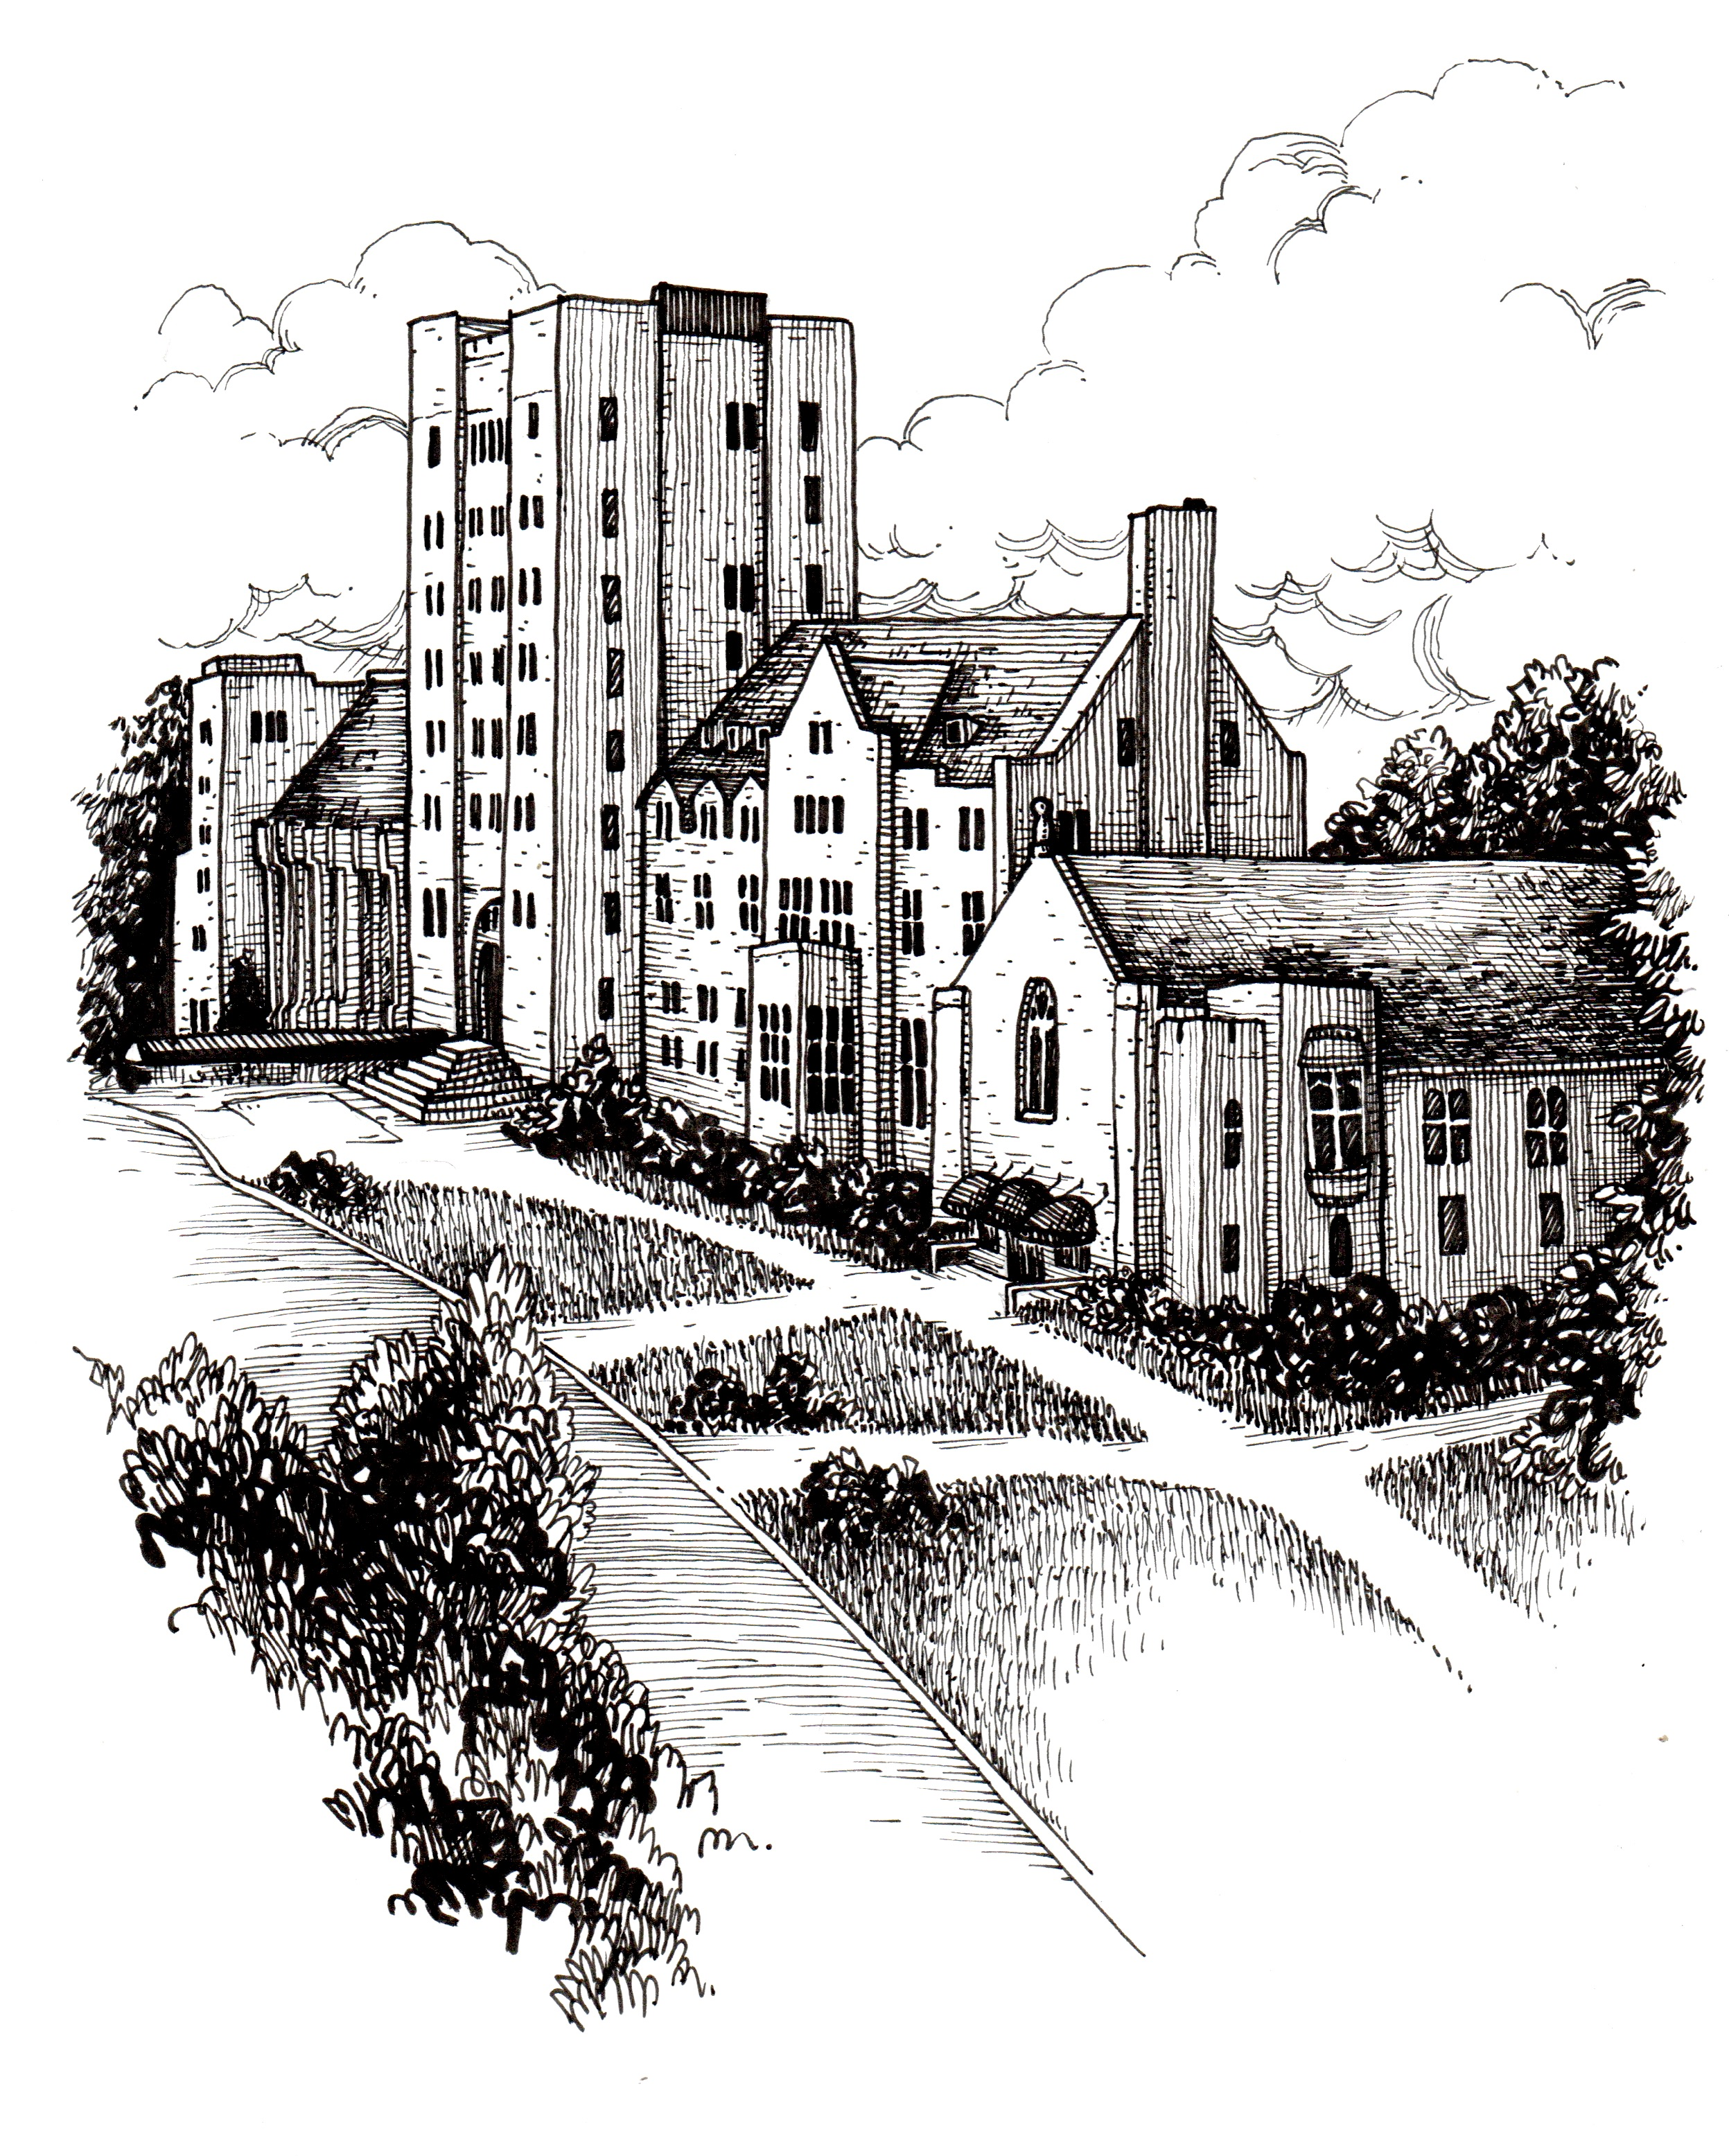
\includegraphics[width=0.6\linewidth,height=\textheight,keepaspectratio]{images/miu5.jpeg}

}

\caption{Indiana Memorial Union}

\end{figure}%

\epigraph{
The numerous symbolic references that have marked the history of universities are also captured in "placemaking." The arrangements and styles of buildings and spaces on a given territory are cultural glue. They attract and fix student and faculty loyalties. In fractured disciplinary environments, they create a sense of the whole being greater than any of its parts. They provide continuity: emotional and sentimental anchors in a world where experiences are fleeting. They unite the generations, keeping graduates close to the institution. 
}
{---Sheldon Rothblatt, "A Note on the 'Integrity' of the University"}

Academic rhythms change slowly---the school calendar and class meeting
times; commencement and summer school; the progression of freshman,
sophomore, junior, senior. The tempo of campus development has a
different cadence, however. As new buildings and facilities are planned,
constructed, and occupied, the calculus of possibilities is always
changing. Likewise, when areas of green nature are marked, modified,
preserved, or enhanced, new horizons of potentiality are revealed. Taken
together, the man-made (human) and the natural (nonhuman) exist in a
dynamic relationship.

As an intentional community of learning, by 1915 IU was settling into
the campus it had occupied for a third of its ninety years as an
institution. One sign of healthy growth was student enrollment, which in
1915 stood at 1,600---eight times as many as in 1885. Handsome limestone
halls were arrayed around the original plot of Dunn's Woods, and the
campus footprint had grown to nearly 120 acres---six times larger than
the original plot in 1885. The academic program was expanding with the
creation of new professional schools and the offering of graduate work.

Concerned about reaching potential students who were not able to come to
the Bloomington campus, President William Bryan established the
Extension Division in 1914, which offered college courses as well as
other educational services to citizens of the state. Aided by the advent
of the automobile to augment the excellent intrastate rail services,
Bloomington faculty traveled to many Indiana cities and towns to offer
classes and programs. The extension programs filled a need, and by the
mid-1920s, the number of statewide enrollments exceeded the student body
in Bloomington.

The Bryan administration took steps to mobilize the growing number of
living alumni. The Society of the Alumni had been formed in 1854 in
response to the devastating campus fire that destroyed the main academic
hall. Since that time, efforts to rouse this group to provide moral and
financial support to the university had been successful but sporadic.
Now there were some two thousand alumni, and their ranks swelled by
several hundred each year at commencement. Keeping alumni informed about
the university as well as their particular graduating class was a key
part of the mobilization strategy. In 1914, a new publication was
launched---the \emph{Indiana University Alumni Quarterly}---designed to
have broad appeal to former students as well as friends of the
university. A special section titled ``Alumni Notes'' in the magazine
was dedicated to news of former students, arranged by graduation year.

In 1915, John W. Cravens, university registrar and secretary to the
board of trustees, wrote a note in the new \emph{Alumni Quarterly} after
the recent purchase of additional land for the campus. He praised the
work of botany professor David Mottier and the campus committee, who had
been helping to enhance the campus landscape by planting native trees
and shrubs for well over a decade. ``As a result,'' Cravens declared,
``Indiana University has one of the most beautiful campuses in the
country. Its hollows, hills, and level places, primeval forests and
recently planted trees, make the campus very attractive. There is a
charm about the campus that stays with one through his entire life. When
a person has once been on the campus of Indiana University he is forever
afterwards enthusiastic about its many entrancing features.''\footnote{\citeproc{ref-cravens1915a}{{``History
  of University Land Purchases,''} \emph{Indiana University Alumni
  Quarterly} 2, no. 2 (1915): 159}; land purchases are summarized in
  \citeproc{ref-myers1952a}{Myers, \emph{History of Indiana University},
  1952, 755}.} Perhaps not surprisingly, an alumnus and employee of
Indiana University expressed these sentiments.

Another former student, novelist Theodore Dreiser, who attended during
the 1889--90 school year, paid a visit to Bloomington in 1915 and
marveled at the changes that had occurred since he last saw the campus
twenty-five years before: ``After this came the university, wholly
changed, but far more attractive than it had been in my day---a really
beautiful school. I could find only a few things---Wylie Hall, the
brook, a portion of some building which had formerly been our library.
It had been so added to that it was scarcely recognizable.''\footnote{\citeproc{ref-dreiser1916a}{\emph{A
  Hoosier Holiday}, 503}. He was referring to Mitchell Hall as the
  former library.} Many new academic halls and supporting infrastructure
served the growing student body, five times the size it was during
Dreiser's day, and the campus footprint had expanded nearly sixfold, to
117 acres.

\section{A New Gymnasium}\label{a-new-gymnasium}

What had begun with the right-angle placement of Owen Hall and Wylie
Hall in 1885 had developed into a large quadrangle, with the center
green provided by trees rather than grass. Orderly rows of buildings
framing the woods were complete on two sides and had been started on the
other two---along Third Street and along Indiana Avenue. The main
entrance to campus remained on Kirkwood Avenue, next to the 1908
University Library. With the recent availability of more campus land
lying northeast of the quadrangle, including the Dunn family homestead,
there was room to grow.

In 1915, the trustees decided that a new gymnasium would be the next
building erected on campus, and they selected a site in the old apple
orchard adjacent to the Dunn family house. To clear the site, the
trustees permitted the students to cut down the trees and create piles
of firewood for bonfires. About half of the student body, numbering
eight hundred or so, showed up on October 21. The day started at the
Student Building with a concert by the university band and a short talk
by President Bryan, who then led the procession to the site. Both the
president and Mrs.~Bryan wielded axes to initiate the cutting. The men
students joined in eagerly, chopping trees and piling wood, while women
students made and served sandwiches. Enough wood was gathered for three
bonfires at pep rallies for football season. IU anatomist and historian
Burton Myers, who was there, later reported: ``This was a joyous
occasion. The students felt that they were helping clear the way for
this long-desired structure.''\footnote{\citeproc{ref-myers1952a}{Myers,
  \emph{History of Indiana University}, 1952, 188}.} In the days
following, the news reported that Bedford attorney Moses Dunn, who sold
the family farm that became the core of IU's campus, had died the day of
the orchard's destruction.\footnote{\citeproc{ref-ehman2010a}{Lee Ehman,
  {``The Dunn Name, but Not the Spirit,''} \emph{Monroe County
  Historian} 3 (August 2010): 10--11}.}

Representing the leading edge of campus expansion, the site was on
Seventh Street, a couple of blocks away from the main part of campus on
Kirkwood Avenue. As the first campus building on the north side of the
stream known as Spanker's Branch---informally referred to as Jordan
River---the gymnasium's imposing Gothic limestone architecture would be
magnified by its site atop a terraced hill, commanding a view to the
west.

With the prospect of new development on campus, President Bryan and the
board of trustees thought it prudent to hire a consultant to prepare a
master plan. Well-known for his work in the park system of Indianapolis,
George Kessler, a landscape architect who worked around the Midwest, had
a thriving business and was engaged in 1915.\footnote{\citeproc{ref-myers1952a}{Myers,
  \emph{History of Indiana University}, 1952, 174}.} In November,
Kessler shared his general ideas for campus planning with President
Bryan and the board of trustees. He thought that ``planning should be
comprehensive. Even though a grand design could only be realized in bits
and pieces, and over a long period of years, still, we should always
know where we are going.''\footnote{Quoted in
  \citeproc{ref-clapacs2017a}{Clapacs, \emph{Indiana University
  Bloomington}, xx}, from Theodore A. Brown and Lyle W. Dorsett, K.C.: A
  History of Kansas City, Missouri (Boulder, CO: Pruett, 1978),
  163--164.} By the following March, Kessler had reported back to the
trustees with some suggestions, including ideas for buildings in the
center of the quadrangle.

In May, President Bryan wrote to Kessler, conveying a diplomatic but
firm message for the preservation of Dunn's Woods:

\begin{quote}
Fully realizing your great ability as an artist, and my own position as
a layman, I nevertheless get my courage together to say that I hope it
may not be thought necessary to place any buildings in the front
quadrangle between the Wylie, Kirkwood, Science line and Indiana Avenue.
Whether the present forest can be replaced by another or not, this great
space seems to me to have more distinction than any building which could
be placed in it. This is the view, I happen to know, of Professor
Brooks, Mr.~Jenkins, the Trustees, and indeed of all of us. I am sure
you would like to have us give you our view whatever it may be
worth.\footnote{\citeproc{ref-bryan1916a}{{``Letter to George Kessler''}
  (Indiana University Archives C286/B150/F Kessler, George, May 25,
  1916)}.}
\end{quote}

Bryan, expressing a clear consensus among the IU academic community,
took the remaining forest off the table for further development. There
was no compelling reason to jettison the existing design of the
thirty-year-old quadrangle.

As plans were developed for the new gymnasium, the entire board of
trustees, along with architect Robert Frost Daggett, visited the site
and the surrounding campus lands. This signaled the aspiration to
coordinate the work of building architects with the efforts of landscape
planners. The completed building, opened in 1917, was thronged with
students at all hours. It served as a lonely architectural sentinel as
future facilities were expected in the recent land purchases northwest
of the quad. In the same period, replanting of the green space
continued. A report indicated that ``32,000 trees had been ordered as
follows: 25,000 yellow poplar seedlings; 2,000 hard maple; 2,000 red
oak; 3,000 pine, spruce, and fir.''\footnote{\citeproc{ref-myers1952a}{Myers,
  \emph{History of Indiana University}, 1952, 206}.}

The care expended on the physical plant was noticed by a distinguished
visitor in 1918. Former US president Theodore Roosevelt visited
Bloomington as the June commencement speaker. The ceremony was held in a
natural ravine converted into an open-air amphitheater, behind Wylie and
Kirkwood Halls. Equipped with a stage and bench seats, the amphitheater
was a gift from the classes of 1909 through 1912.\footnote{\citeproc{ref-clapacs2017a}{Clapacs,
  \emph{Indiana University Bloomington}, 166--67}.} The former president
began his remarks:

\begin{quote}
I want to say at the outset that I don't think I have ever been at a
more beautiful university commencement than this. I shall always keep in
mind this scene here in the open by the university buildings, a
university which\ldots is approaching its centenary, here under these
great trees, these maples and beeches, that have survived over from the
primeval forest, to see all of you here and the graduating class
composed mainly of girls this year---it is a sight I shall never
forget,---it will always be with me.\footnote{\citeproc{ref-roosevelt1918a}{{``Straightout
  Americanism,''} \emph{Indiana University Alumni Quarterly} 5, no. 3
  (July 1918): 295--307}.}
\end{quote}

President Roosevelt expressed what students, staff, alumni, and other
visitors already knew and appreciated about the campus.

In 1922, another distinguished visitor came to campus and stayed awhile.
Theodore Clement Steele (T. C. Steele), a well-known painter from the
art colony in neighboring Brown County, was appointed honorary professor
of painting. He had a long association with the campus, painting
portraits of many IU faculty, President Bryan among them, before turning
to landscape interpretations. Bryan's idea was that Steele's very
presence would help stimulate art appreciation on campus, thus
contributing to the moral uplift of the student body. For his part,
Steele rendered his mission to the students in a straightforward way:
``to see the Beautiful in nature and life.''\footnote{\citeproc{ref-capshew2012a}{Capshew,
  \emph{Herman {B} Wells}, 27}.}

The university provided studio space in the attic of the main library,
above the large reading room. During his residency, Steele and his wife,
Selma, spent the winters in Bloomington and the summers in Brown County,
at their home near Belmont. The artist was modest and unpretentious
about his work, and he welcomed visitors dropping in when the studio was
open on Thursday, Friday, and Saturday each week. During clement
weather, Steele set up his easel outdoors and painted \emph{en plein
air}. The resulting canvases showed different campus buildings, such as
the Student Building and Kirkwood Observatory, and landscape features,
such as the central woods and the Jordan River. In 1923, the Union Board
bought six of Steele's paintings, which provided the nucleus for the art
collection of the Indiana Memorial Union. Although his original term as
honorary professor was meant to last only a year, he stayed on happily
until 1926, the year of his death.\footnote{\citeproc{ref-capshew2012a}{Capshew,
  27--29}. The IMU now owns over seventy paintings of T. C. Steele.}

\section{Campuses, the Old and the
New}\label{campuses-the-old-and-the-new}

To mark the centennial of the first buildings on the old campus, in
1922, administrative factotum John Cravens penned a series of three
articles for the \emph{Alumni Quarterly}. By that time, the university
had been occupying the campus at Dunn's Wood for a third of a century. A
former school superintendent and court clerk for Monroe County, Cravens
occupied a unique position in the university. Appointed as IU registrar
in 1895, he became the secretary to the board of trustees in 1898
concurrently. In 1915, he added another duty---secretary of the
university. Thus, Cravens played a key role in gatekeeping for the
student body and witnessing trustee decision-making. As the trustee
board authorized campus infrastructure driven by the needs of the
student body, Cravens had access to relevant records of IU's building
program as he wrote ``Buildings on the Old and New Campuses of Indiana
University.''\footnote{\citeproc{ref-cravens1922b}{John W. Cravens,
  {``Buildings on the Old and New Campuses of Indiana University: I. The
  Old Seminary Building,''} \emph{Indiana University Alumni Quarterly}
  9, no. 1 (1922): 1--11}; \citeproc{ref-cravens1922a}{Cravens,
  {``Buildings on the Old and New Campuses of Indiana University,''}
  1922}; \citeproc{ref-cravens1922c}{John W. Cravens, {``Buildings on
  the Old and New Campuses of Indiana University: III. Buildings on the
  New Campus and Elsewhere in Monroe County,''} \emph{Indiana University
  Alumni Quarterly} 9, no. 3 (1922): 303--20}.}

He started, not surprisingly, with the original Seminary Building on the
old campus. Cravens intoned reverently: ``What a train of thoughts comes
to one when he stands on the very site which marks the beginning of that
institution destined to become in law and in fact `the head of Indiana's
public-school system.' One feels that he should stand here with
uncovered head. San Salvador, Plymouth Rock, and Jamestown each has its
special significance. Each was the beginning of an important movement.
The Old Seminary Building is the cradle of higher education in
Indiana.''\footnote{\citeproc{ref-cravens1922b}{Cravens, {``Buildings on
  the Old and New Campuses of Indiana University,''} 1922, 1}.} He went
on to describe the process of choosing the site and the details of
construction of the simple two-story brick structure, then launched into
a description of the building's uses over time and listed many of the
early graduates who had made names for themselves. As the only academic
building, it saw constant use from 1824 to 1836. When the larger College
Building was finished in 1836, the older building was pressed into
service as needs arose. It was torn down in 1858.

Cravens was attempting a word portrait, to fix in the reader's mind the
primordial significance of the structure that was the first physical
embodiment of the idea of Indiana University. The trouble was, he
admitted, ``the \emph{exact} location of the Old Seminary Building had
passed from the memories of the oldest graduates and citizens of
Bloomington'' in the two-thirds of a century since it was demolished.
People remembered it was ``\,`on the high ground near the southwest
corner of the old campus,' but all outward traces of the building had
disappeared.''\footnote{\citeproc{ref-cravens1922b}{Cravens, 3}.
  Original emphasis.} Undeterred, Cravens got permission and a crew of
men to excavate for any remains of the original building.

Charles Hays, the assistant superintendent of buildings and grounds, was
the foreman.\footnote{Charles H. Hays (1897--1937) was a native of
  Monroe County and spent a thirty-one-year career at the university.
  Starting in 1906 as a custodian for Kirkwood Hall, he became assistant
  superintendent of buildings and grounds in 1917. After being promoted
  to superintendent at the death of his predecessor, Eugene Kerr, in
  1926, he served until his sudden death from a heart attack in 1937.
  President Bryan noted his artistic interests, which took various
  forms: scenery manager for student plays, decorator for university
  events, and campus landscape designer. See
  \citeproc{ref-iuaq1937a}{{``{Charles H. Hays},''} \emph{Indiana
  University Alumni Quarterly} 24 (1937): 511--12}.} In addition to the
university work crew, a group of older residents of Bloomington served
as location consultants, including Hays's father-in-law, who pointed to
a spot within fifteen feet of where the old building had stood. They
discovered the ruins of the Seminary Building, unearthing part of the
foundation and entrance steps, and found the base of the College
Building, which was constructed in 1836 and destroyed by fire in 1854.
They marked the location with a stone and considered the construction of
a suitable monument.\footnote{\citeproc{ref-ids1922a}{{``Discover Ruins
  of Seminary Building,''} \emph{Indiana Daily Student}, January 18,
  1922, 3}. See map in Cravens, \citeproc{ref-cravens1922a}{{``Buildings
  on the Old and New Campuses of Indiana University,''} 1922}, p.~161.}

In his second article, Cravens covered the remaining six buildings on
the original campus---the professor's house (1824--1864), the College
Building (1836--1854), the Boarding-House (1838--1864), the Laboratory
Building (1840--1858), the second College Building (1855--present), and
Science Hall (1873--1883)---with details of construction and
use.\footnote{The second College Building, sometimes referred to as the
  first University Building, was sold to the Bloomington school system
  in 1897 and served as Bloomington High School until 1965, when a new
  school was opened at 1965 S. Walnut Street and the former IU building
  was razed.} He delineated the trustee board's debate after the fire
that destroyed Science Hall in July 1883, about whether to rebuild on
the seminary site. In September 1883, the trustees entertained seven
sites, including the existing campus, ranging from ten to fifty acres.
After discussion, a test vote was taken, with three favoring the present
site, three for the Blair property (located northwest), and one for the
Dunn property (located east). After further debate, the final vote was
taken, with five for Dunn's Woods and three for the existing site.
Cravens summarized: ``And thus our present magnificent campus,
recognized as one of the finest in the United States, was
selected.''\footnote{\citeproc{ref-cravens1922a}{{``Buildings on the Old
  and New Campuses of Indiana University,''} 1922, 164}.}

Cravens then went on to recount the story of the first buildings on the
new campus in the third article, starting with Wylie Hall and Owen Hall,
that eventually formed ``three sides of a quadrangle on the crest of the
campus proper.''\footnote{\citeproc{ref-cravens1922c}{{``Buildings on
  the Old and New Campuses of Indiana University,''} 1922}.} He
enumerated in order of construction the seventeen buildings and
structures that populated the campus in 1922, nearly thirty-five years
after the move to Dunn's Woods. He noted that all except two of the
trustees who engineered the relocation were deceased. In each of the
capsule histories, Cravens gave a myriad of architectural, construction,
and financial details, in addition to the naming of the building,
whether functional (Power Plant No.~1 or Student Building) or honorary
(Maxwell Hall or Kirkwood Observatory). The result was a trove of rare
information, combining data from records but also from campus lore and
personal observation. The article ended with the newest building, the
Commerce and Finance Building, for the use of the recently founded
School of Commerce and Finance, which was still under construction in
1922.\footnote{\citeproc{ref-cravens1922c}{Cravens, 319--20}. The
  Commerce and Finance Building was renamed William A. Rawles Hall in
  1963 by the trustees.}

Cravens's series, coming on the heels of IU's centennial in 1920, was a
unique compendium of campus architectural and social history. It married
the old and new campuses in a straightforward chronicle of institutional
progress, in which the devastating fires on the old campus served as an
impetus for the relocation and led to brighter prospects for the
university. The hidden variable in this focus on the physical plant was
an exponential increase in the size of the student body, from less than
two hundred at the start of the 1880s to nearly three thousand in 1922,
with a concomitant expansion of faculty and staff numbers. The
escalating growth of the campus infrastructure was also a result. Not
only did Cravens's articles draw attention to this formative period of
campus development in its material embodiment, but they were also a
refreshing complement to the exclusive focus on educational philosophy,
policy, and practice that was found in the \emph{Centennial Memorial
Volume} published in 1921.\footnote{\citeproc{ref-chamness1921a}{Chamness,
  \emph{Indiana University, 1820--1920}}.}

\section{Literary Appreciations}\label{literary-appreciations}

As enrollments kept rising through the 1920s, from 2,300 to 3,500
students, a remarkable efflorescence of prose occurred among students
that featured the Bloomington campus. Whether addressing their
remembered or present experience, student writers described the weather,
the trees, and the buildings and pathways, thus evoking the university's
unique spirit of place. Some evidenced a deep attachment to place;
others used the campus as a setting to describe personal feelings or
states of mind.

Ernie Pyle, a columnist and editor for the \emph{Indiana Daily Student},
penned a paean to IU's spirit of place as students were returning to
classes for the 1922 fall semester:

\begin{quote}
Nearly everyone who has ever attended Indiana University will tell you
there is no place in the world like Indiana. They sometimes attempt to
explain that statement but they cannot. When they ejaculate that there
is no place in all the world like Indiana, they are thinking about
something else. They are thinking about spring days when the campus is
bursting with fragrance, vivid with color of blossoms and new leaves,
and then the moon is bright---it is undeniable that spring is nowhere in
the world as it is at Indiana. They are thinking about autumn evenings
when dusk has settled.
\end{quote}

Moving from the ambiance of nature to the human milieu, Pyle observed
the deep interpersonal attachments the college experience fostered,
continuing: ``They are thinking about hundreds of wholesome, pleasant
people, who were their friends. They are thinking something about
Indiana which none of them could ever express in words. These persons
who make such broad unqualified statements about Indiana say that they
have since tried living in many other places but somehow that tang is
missing.''\footnote{\citeproc{ref-pyle1922a}{Ernie Pyle, {``It's in the
  Air,''} \emph{Indiana Daily Student}, September 5, 1922, 4}.} Trying
to grapple with an ineffable spirit of place, Pyle showed glimpses of
his gift for description and his penchant to take the ordinary
universals of life as his subject.

Another student of the 1920s shaped by his time on the Bloomington
campus was Hoagy Carmichael, who wrote about the main student hangout in
a memoir. Located across the street from the campus, the Book Nook, a
former bookstore turned into a soda fountain, was ``the hub of all
student activity'' in the days before the Indiana Memorial
Union.\footnote{\citeproc{ref-wells1980a}{Wells, \emph{Being Lucky},
  33}.} Carmichael later recalled the teeming social life---indelibly
associated with the composition of ``Stardust''---contained within:

\begin{quote}
On Indiana Avenue stood the Book Nook, a randy temple smelling of socks,
wet slickers, vanilla flavoring, face powder, and unread books. Its dim
lights, its scarred walls, its marked-up booths, unsteady tables, make
campus history. It was for us King Arthur's Round Table, a wailing wall,
a fortune telling tent. It tried to be a bookstore. It had grown and
been added to recklessly until by the time I was a senior in high school
it seated a hundred or so Coke-guzzling, book-annoyed, bug-eyed college
students. New tunes were heard and praised or thumbed down, lengthy
discussions on sex, drama, sport, money, and motor cars were started and
never quite finished. The first steps of the toddle, the shimmy, and the
strut were taken and fitted to the new rhythms. Dates were made and mad
hopes were born.\footnote{Hoagy Carmichael and Stephen Longstreet,
  \citeproc{ref-carmichael1965a}{\emph{Sometimes i Wonder: The Story of
  Hoagy Carmichael} (New York: Farrer, Straus; Giroux, 1965)},
  pp.~54--55. To sort out the folklore surrounding the composition of
  ``Stardust,'' see Richard M. Sudhalter,
  \citeproc{ref-sudhalter2002a}{\emph{Stardust Melody: The Life and
  Music of Hoagy Carmichael} (New York: Oxford University Press, 2002)},
  pp.~103--123.}
\end{quote}

Carmichael, a Bloomington native, had a special feel for his home in a
college town. In his first, impressionistic memoir, published in 1946,
he described the campus as he remembered it in the 1920s:

\begin{quote}
A low stone wall borders the campus on the south. This is the ``spooning
wall'' and it is usually dotted by quiet indiscernible couples late at
night who have stopped there on the way home from the Book Nook or a
picture show. To the north of the campus, bounding Dunn Meadows
{[}\emph{sic}{]} and the old athletic fields, runs the famous Jordan
River. Famous because of its high-sounding name and yet its waters---a
foot deep in floodtime---barely trickle during the dog days of
August.\footnote{\citeproc{ref-carmichael1969a}{Hoagy Carmichael,
  \emph{The Stardust Road} (1946; repr., New York: Greenwood Press,
  1969), 34}.}
\end{quote}

Tinged with nostalgia about times past, more wistful than sentimental,
Carmichael's writing was retrospective as he recalled his Bloomington
roots years later.

For the first time, the campus woodland was the setting for a novel.
Published in 1925, the novel \emph{Initiation} was written by George J.
Shively, a member of the class of 1916 who majored in
English.\footnote{George J. Shively (1892--1980) was the son of Benjamin
  Franklin Shively (1857--1916), a US senator (1909--16) and IU trustee
  (1893--1916) who served as president of the board from 1906 until his
  death. He died on March 14, 1916, when his son George was weeks away
  from IU graduation.} A coming-of-age story, much of the action took
place on university grounds under a fictionalized name for the
institution. \emph{The Vagabond}, the campus literary magazine,
enthused: ``For the first time Indiana University lives under its own
name and at full length in modern fiction. The veil is frankly not drawn
over reality by calling the place Monrovia College and renaming Jordan
Field. It deals with Indiana University more openly than does the
University catalogue. Any student or alumnus knows where he is\ldots. It
is by far the best description of student life so far written about the
school.''\footnote{\citeproc{ref-fcs1925a}{F. C. S{[}enour{]}, {``A
  Novel of Indiana University,''} \emph{The Vagabond} 2, no. 3 (March
  1925): 51--52}.}

Following graduation, Shively went to Yale University to pursue literary
studies, but after a year, his graduate program was interrupted by the
Great War in Europe. He served in the Yale ambulance unit with the
French Army during the war, where he was wounded. His first publication,
a concise history of his ambulance unit, came out in 1920.\footnote{\citeproc{ref-shively1920a}{George
  J. Shively, ed., \emph{Record of {S.S.U.} 585} (New Haven: Brick Row
  Book Shop, 1920)}.}

\emph{Initiation} was his second publication. As described in the novel,
his recollections of IU campus life were fresh and vivid, tinged with
longing for a more innocent time:

\begin{quote}
Upon John grew that affection which no one can escape who walks long
under campus trees; that naïve and sentimental fondness at once fatuous
and deep, that clings to a man long afterward, and that has been known,
of mention of Alma Mater, to show up soft in gnarled citizens otherwise
hard-shelled as the devil himself. To a peculiar degree the Indiana
milieu was created to inspire love. It has the unspoiled generosity, the
frankness, the toil, the taciturn courage and the exasperating ineptness
of natural man himself. One listens to the winds sighing through
beeches, or plods through autumnal drizzle with gaze divided between the
cracks of the Board Walk and that miraculous personal vision that for no
two people is produced alike, whether it be conjured from books, or from
inner song, or from liquor, or from a co-ed's smile or from all
together. Because of this one berates Indiana and loves her
doggedly.\footnote{\citeproc{ref-shivley1925a}{George Shively,
  \emph{Initiation} (New York: Harcourt, Brace; Company, 1925), 122}.}
\end{quote}

Shively went on to publish one other novel, \emph{Sabbatical Year}
(1926), a saga of an upper-class American family, before making a career
in the publishing industry as a senior editor at Doubleday \& Company in
New York.\footnote{See
  \href{https://www.nytimes.com/1973/02/06/archives/mrs-george-shively.html?smid=url-share}{``Mrs.~George
  Shively''}}

In 1929, writer and humorist Don Herold penned a remembrance of his
student days. Originally from Bloomfield, in a neighboring county,
Herold graduated in 1913. He stated:

\begin{quote}
It is hard not to get soft about the Indiana campus. I know of none in
America which surpasses it in beauty. Indiana buildings, some good, many
architecturally atrocious, have been set in a forest of fine old trees,
as the real estate agents would say. No adolescent saplings these, but
grand old patriarch timber to touch the souls of sensitive boys and
girls. I think the really worthwhile college student is a bit sad, and I
feel that every campus should offer the comfort of towering trees. I am
glad I did not have to go to college in a skyscraper or on a sun-baked
subdivision. Romance burns best on a wooded campus. It would take a
pretty generous state appropriation to offset the thrill of a stroll on
the board walk from Kirkwood Hall to Forest Place\ldots. As I said to
myself a lot of times, say I, ``I like this campus,'' and I know every
other Indiana undergraduate has had many a similar throb.\footnote{\citeproc{ref-herold1929a}{Don
  Herold, \emph{College Humor}, November 1929, 130--31}.}
\end{quote}

Such literary appreciations describe the emotional pull of the campus,
heightened by campus society and the developmental challenges of
learning and study.

Other students, less self-consciously literary, left their impressions
as well. When Eura Ann Sargent, from Indianapolis, came to IU as a
first-year student in 1927, the campus was largely as Cravens described
it a few years before. The physical plant consisted of about a dozen
academic halls arranged around three sides of Dunn's Woods, plus the old
Assembly Hall, power plant, and the new Men's Gymnasium. All except the
new gymnasium were adjacent to the woods. She remembered:

\begin{quote}
The campus was a thing of beauty. All around the Well House to the
street was colorful woods. The sun had to force its way through the
dense foliage and soft breezes stirred the leaves to make lazy ephemeral
shadows on a ground carpeted with some of last year's leaves and dotted
with a few wild flowers and other stirring sprouts which dared to live
in spite of the shade. Behind most of these ten buildings was
picturesque and natural growth. Nature seemed to be pleased to have such
latitude and was doing her utmost to make the best of the
opportunity.\footnote{Sargent interview, in IU Archives reference file
  ``African Americans at IU. William Smith's Research Files for the
  `African American Experience at IU' Project.'' Sargent was among the
  tiny minority of African Americans at IU during this period, about 1
  percent.}
\end{quote}

Sargent joined generations of students who responded to the beauty of
the campus and the intermingling of stone buildings and the woodland.

Among those responsible for the physical plant in those times was
Charles Hays, then assistant superintendent of building and grounds. He
not only supervised the groundskeepers but also tried his hand in
landscape design. Because bedrock was located close to the surface in
Bloomington, there were small-scale limestone quarries dotting the area.
One was on campus near Third Street, west of Memorial Hall, sometimes
called Dunn Quarry.

In 1928, Hays designed a rock garden within the old quarry, featuring a
pond and attractive landscaping. The Sunken Gardens became ``one of the
most beautiful spots on campus,'' and the classes of 1927 and 1928
contributed money for supplies.\footnote{\citeproc{ref-myers1952a}{Myers,
  \emph{History of Indiana University}, 1952, 381};
  \citeproc{ref-iuaq1937a}{{``{Charles H. Hays},''} 1937};
  \citeproc{ref-iam1957a}{{``{Charles H. Hays},''} \emph{Indiana Alumni
  Magazine} 19, no. 7 (1957): 1}.} A local resident vividly remembered
playing there as a child:

\begin{quote}
It is still a refuge, a playground, a Paradise. Two arches in a low
stone wall invite entry to descending flights of rough, shallow steps.
These are bordered by trees, ferns and ground cover plants which hold
the cool, dark, damp atmosphere born of the wide pond at the foot of
steps. Circling the pond, the questing child arrives at her goal---the
huge, sloping limestone rock which juts into the water. The rock's
surface, about two feet above the water, is superbly placed for watching
crawdads and water striders, and is itself studded with fossils. The
cool quiet of the Sunken Gardens was then, and is now, that child's safe
haven.\footnote{\citeproc{ref-gabbay2013a}{Sue Davis Gabbay, {``Letter
  to Brad Cook''} (Indiana University Archives/Reference file: B+G
  Sunken Gardens, March 2013)}.}
\end{quote}

Heavily used by sunbathers, swimmers, and artists, it was also favored
by college sweethearts, leading to its popular name, the Passion Pit.
For over two decades, the gardens provided a tranquil and picturesque
setting for communing with nature until they were removed to make way
for the construction of Jordan Hall (now Biology Hall) in the early
1950s.\footnote{See \citeproc{ref-clapacs2017a}{Clapacs, \emph{Indiana
  University Bloomington}, 181}.}

In 1929, alumna Edith Hennel Ellis, a member of the class of 1911,
authored an article about the woodland campus for the \emph{Alumni
Quarterly}. Simply titled ``The Trees on the I.U. Campus,'' it included
poetic descriptions: ``Certain scenes stamp themselves indelibly upon
the mind: lingering shadows of tall trees creeping across the grass on
long summer afternoons; black trunks of trees rising from snow-covered
slopes, etched against a leaden winter sky; masses of Forsythia bursting
into sudden yellow bloom; and that loveliest of all Indiana springtime
pictures, white dogwood and pink redbud blooming against a green
background of maples.'' Ellis asserted: ``The Indiana University campus
is famous the country over for its natural beauty. It is more than a
thing of beauty. Its trees are sanctuaries under which old men may dream
dreams and young men may see visions.''\footnote{\citeproc{ref-ellis1929a}{Ellis,
  {``{The Trees on the I.U. Campus},''} 331}.}

\section{Campus Development in the 1920s and
1930s}\label{campus-development-in-the-1920s-and-1930s}

The landscape architectural firm of Olmsted Brothers began consulting
with the IU administration in 1929.\footnote{In 1898, John Charles
  Olmsted (1852--1920) and Frederick Law Olmsted Jr.~(1870--1957) formed
  the Olmsted Brothers partnership, operating under that name until
  1961. See
  \href{http://www.olmsted.org/the-olmsted-legacy/the-olmsted-firm/an-introduction}{Olmstead
  Firm}.} They prepared site plans for proposed buildings, laid out
paths and streets, and advised on landscape design and planting schemes.
They also carefully inventoried trees and vegetation in Dunn's Wood,
with a blueprint of location, species, and size. Like before, IU
officials used the plans as guidelines and suggestions, modifying their
implementation according to available finances and current priorities.

After the Men's Gymnasium on Seventh Street opened in 1917, other new
buildings sprang up during the 1920s. The first was on the quadrangle:
the Commerce Building (now Rawles Hall), completed in 1923, due east of
the Biology Hall (now Swain Hall East) on Third Street. To mark a
primary entrance to the building, the class of 1926 donated funds for a
pair of limestone pillars on the sidewalk adjacent to Third Street. In
1924, a campus home for President Bryan and his wife, Charlotte Lowe
Bryan, was constructed. It was east of the quadrangle, along the campus
border, on a slight rise between two small creeks. It was known as the
President's House (now Bryan House).

It was the last construction project overseen by Superintendent of
Buildings and Grounds Eugene Kerr, who died in July. The \emph{Indiana
Daily Student} noted Kerr's passing: ``For the last twenty years this
man has labored earnestly for the good and advancement of the
University. He has been instrumental in bringing about many of the
needed improvements in buildings and grounds during that time. He took
deep pride in keeping the buildings and grounds in the best of
condition, and largely through his efforts the campus still ranks as one
of the most beautiful of any college or university in
America.''\footnote{Quoted in \citeproc{ref-iuaq1924a}{{``Death of
  Eugene Kerr,''} \emph{Indiana University Alumni Quarterly} 11, no. 4
  (1924): 544}.} After Kerr's death, Charles Hays stepped into the role
of superintendent of buildings and grounds and served from 1924 to 1937.
A few months later, Kerr was memorialized by a bronze plaque placed in
Maxwell Hall.\footnote{\citeproc{ref-botm1925a}{Indiana University Board
  of Trustees, {``Minutes of the Board of Trustees of Indiana
  University, 13 March 1925--14 March 1925''} (Bloomington: Indiana
  University Archives \& Indiana University Libraries Digital
  Collections Services, March 14, 1925),
  \url{https://purl.dlib.indiana.edu/iudl/archives/iubot/1925-03-13}}.}

Also in 1924, the first dormitory for men, South Hall (now Smith Hall),
was opened on Tenth Street, colonizing yet another street for the campus
building program. It was joined the following year by Memorial Stadium
(now Cox Arboretum) to the east. Across campus on Third Street, the
first dormitory for women, Memorial Hall, was finished in 1925. It was
no accident that living quarters for women and for men were on opposite
ends of campus. In 1928, athletic facilities were boosted by the
construction of the huge Fieldhouse (now the Garrett Fieldhouse),
attached to the Men's Gym, suitable for intercollegiate sports.

Despite the stock market crash in 1929, campus construction continued.
That year, the power plant was renovated after a fire and finally made
adequate.\footnote{\citeproc{ref-myers1952a}{Myers, \emph{History of
  Indiana University}, 1952, 764}.} The class of 1929 funded a set of
limestone gates along the campus border on Third Street, between Biology
Hall (now Swain East) and Commerce Building (now Rawles
Hall).\footnote{\citeproc{ref-iu_classgifts}{Indiana University
  Archives, {``Reference File: Class Gifts''} (Bloomington: Indiana
  University; Unpublished archival material, n.d.)}.}

In 1931, the long-planned Chemistry Building was completed. The large
and handsome limestone building, decorated with a bold frieze depicting
the elements of the periodic table punctuated with clusters of grapes,
occupied a site due east of Wylie and Kirkwood Halls, outside of the
quadrangle. The well-used amphitheater, the location of many
commencement ceremonies and convocation programs, had to be sacrificed
to make room for the new building, although one can still see the
remnants of the natural ravine near the north entrance.\footnote{\citeproc{ref-myers1952a}{Myers,
  \emph{History of Indiana University}, 1952, 418--19, 434--35};
  \citeproc{ref-lyon1931a}{Robert E. Lyon, {``The History of Chemistry
  at Indiana University, 1829--1931,''} \emph{Indiana University
  News-Letter} 19, no. 3 (March 1931)}.}

The last of the facilities financed by the Memorial Fund was the Indiana
Memorial Union (IMU). Formally dedicated at commencement in June 1932
with an inaugural dinner in Alumni Hall, the building was located south
of Jordan River and north of Maxwell Hall, a few steps away from the
quadrangle. Richly ornamented limestone carvings embellished the
exterior, and the main Romanesque tower rivaled the tallest building in
downtown Bloomington a few blocks away. In the lobby, a bronze tablet in
the floor depicted the different branches of the military services of
the IU men and women memorialized by the building and the Golden Book
listed the names of those who served as well as the contributors who
donated to the Memorial Fund drive. (Since 1961, the bronze tablet and
the Golden Book have been located in the Memorial Room, an antechamber
off the lobby.) The east wing was allocated for the university
bookstore, which featured a second-floor balcony and lounge with a
fireplace. Taken with the graceful luxuriance of its utilitarian design,
President Bryan boasted that it was ``the most beautiful college
bookstore in America.'' The bookstore manager, Ward G. Biddle, became
the first director of the Indiana Memorial Union. Almost immediately,
the union became an essential part of campus life as well as an iconic
architectural landmark.\footnote{Myers,
  \citeproc{ref-myers1952a}{\emph{History of Indiana University}, 1952},
  pp.~413--417; Clapacs, \citeproc{ref-clapacs2017a}{\emph{Indiana
  University Bloomington}}, pp.~266--271;
  \href{https://goldenbook.iu.edu/}{The Golden Book}}

Two months following the IMU dedication, the national economic situation
caught up to the Hoosier economy, and the Indiana General Assembly cut
Indiana University's budget request by 15 percent. Soon after, the Bryan
administration authorized faculty salary reductions ranging from 8
percent to 12.5 percent. President Bryan, who insisted on an even higher
cut to his own salary, received expressions of gratitude from the
faculty that the reductions were not higher.\footnote{\citeproc{ref-myers1952a}{Myers,
  \emph{History of Indiana University}, 1952, 436--39}.}

It was years before the situation improved. In 1935, the university
presented a budget to the state of just under \$1.5 million, which was
met with success, accompanied by a supplemental request of \$335,000 to
address deferred needs, which was not. The next year, President Bryan
prepared the budget request, noting that salaries had not been restored
after the 1932 cut. The state granted \$1.9 million in 1937, about 15
percent less than the request, and did not fund the requested \$500,000
for capital projects.\footnote{\citeproc{ref-myers1952a}{Myers, 504--7}.}

The federal government, under President Franklin Roosevelt, had several
relief agencies operating during the 1930s to assist in providing funds
for public works, notably the Public Works Administration (PWA) and the
Works Progress Administration (WPA, later Work Projects Administration).
Revising previous lists of building needs, in 1935, the trustees sought
federal assistance for an extension of the power plant, another women's
dormitory, and buildings for the music school, education school,
university administration, and one each for the medical school in
Bloomington and in Indianapolis. The state government, under Governor
Paul McNutt, former dean of the IU School of Law, assisted in obtaining
financing.\footnote{\citeproc{ref-myers1952a}{Myers, 515--31}.}

As the trustees prepared to finance construction of a new administration
building in 1935 with the aid of WPA funds, they decided to put it east
of Kirkwood Observatory and north of Fourth Street---right in the center
of the woods.\footnote{\citeproc{ref-botm1935a}{Indiana University Board
  of Trustees, {``Minutes of the Board of Trustees of Indiana
  University, 04 March 1935''} (Bloomington: Indiana University Archives
  \& Indiana University Libraries Digital Collections Services, March 4,
  1935),
  \url{https://purl.dlib.indiana.edu/iudl/archives/iubot/1935-03-04}}.}
Students got wind of this plan and expressed their misgivings through
the editorial columns of the \emph{Indiana Daily Student} newspaper.
There was general concern that it would mar the natural beauty of the
campus. Zoology professor Alfred Kinsey sided with the students opposing
the plan, but English professor William Jenkins supported placing the
building in Dunn's Woods.

The newspaper published each of their statements in full. Jenkins cited
the opinions of experts, arguing that ``every survey of the campus by
qualified landscape architects has put the building on that site.'' He
thought most people could imagine seeing the gray limestone structure
half hidden by the trees from Maxwell Hall. Besides, he thought, it was
a common error to think that forest trees are desirable near a formal
building. ``As a matter of fact such a building should have formally
treated grounds about it,'' he concluded. Kinsey, who was an
accomplished botanist as well as a zoologist, drew an analogy: ``From a
landscape standpoint it is better that the center of the campus be kept
clear of buildings for the same reason that the center of a lawn should
be kept clear of shrubbery and flower beds.'' He reminded readers that
the central quadrangle, under development for a half century, had been
framed on two and a half sides with perimeter buildings. ``The heart of
the picture is the growth of trees which has made our campus famous all
over the country.'' Barring some new comprehensive plan, he argued,
``new buildings should be placed to complete three or four sides of the
picture without modifying the present center of that
picture.''\footnote{\citeproc{ref-ids1935a}{{``Professors Take Divergent
  Views on Building Site,''} \emph{Indiana Daily Student}, March 28,
  1935, 1, 3}.}

The concerns of students and faculty resonated with the trustees, and
they relocated the plans for the administration building to the corner
of Indiana and Kirkwood Avenues, due south of the library, making a
start on the fourth side of the quadrangle's framing.\footnote{\citeproc{ref-botm1935b}{Indiana
  University Board of Trustees, {``Minutes of the Board of Trustees of
  Indiana University, 04 April 1935''} (Bloomington: Indiana University
  Archives \& Indiana University Libraries Digital Collections Services,
  April 4, 1935),
  \url{https://purl.dlib.indiana.edu/iudl/archives/iubot/1935-04-04}}.}
The administration building, officially named for President William Lowe
Bryan in 1936 at the urging of Governor McNutt, was called by its
generic name because PWA rules prevented the use of Bryan's name during
his lifetime.\footnote{\citeproc{ref-myers1952a}{Myers, \emph{History of
  Indiana University}, 1952, 523}.} The class of 1935 provided funds for
limestone benches on the first and second floors.\footnote{\citeproc{ref-iu_classgifts}{Indiana
  University Archives, {``Reference File''}}.}

In 1937, three new buildings were completed: a women's dormitory
(Goodbody Hall), placed at right angles to Memorial Hall, and the School
of Music Building (now Merrill Hall) and the Medical Building (now Myers
Hall), both along Third Street. The next year, the Clinical Building of
the School of Medicine was completed in Indianapolis, and the School of
Education Building, including a laboratory school, University School,
was finished, located at the corner of Third Street and Jordan Avenue,
anchoring the growing line of university buildings on Third Street
stretching westward to Indiana Avenue.\footnote{\citeproc{ref-myers1952a}{Myers,
  \emph{History of Indiana University}, 1952, 515--31}.}

\section{Beneath the Sundial}\label{beneath-the-sundial}

Amid this forward-looking expansion, pieces of the campus's past also
sprung up. Otto and Mathilda Klopsch were both members of the class of
1896, the year the sundial was relocated from the old campus to Dunn's
Woods. They had fond memories of the woodland campus and reminisced
about their time at IU with their three children. In 1935, after both
had died, their son Otto Jr.~requested and received permission from
President Bryan to scatter their ashes at the base of the sundial. Their
children made a wish: ``May their spirit rest as peacefully as it lived
happily while they studied and loved on these grounds.'' A bronze plaque
at the sundial's base was inscribed:

\begin{quote}
Mathilda Zwicker Klopsch / Otto Paul Klopsch / Class of 1896\\
They met at this sundial when classmates.\\
Their ashes rest here together until eternity.
\end{quote}

This memorial joined Dunn Cemetery as a consecrated place of memory on
the IU campus.\footnote{\citeproc{ref-clapacs2017a}{Clapacs,
  \emph{Indiana University Bloomington}, 324};
  \citeproc{ref-lesnick2005a}{Gavin Lesnick, {``Campus Icon Retains
  History, Myth from 1868,''} \emph{Indiana Daily Student}, September
  13, 2005,
  \url{https://www.idsnews.com/article/2005/09/campus-icon-retains-history-myth-from-1868}}.}

Keeper of Grounds William Ogg turned eighty in 1931 but continued
working throughout the decade. In 1936, President Bryan lauded Ogg as a
``master of the fine arts of dealing with all things that grow upon our
glorious campus'' for the previous thirty-five years: ``Dealing rightly
with plants is Art.''\footnote{Bryan quoted in
  \citeproc{ref-iuaq1936a}{{``{In Memoriam: William A. Rawles, '84,
  Robert A. Ogg, '72, William T. Patten, '93; and Necrology List},''}
  309--10}.} In 1938, Ogg finally got out of the weather and became the
``greenhouse man,'' with his salary line transferred to the Department
of Botany.\footnote{\citeproc{ref-botm1938a}{Indiana University Board of
  Trustees, {``Minutes of the Board of Trustees of Indiana University,
  03 November 1938--04 November 1938''} (Bloomington: Indiana University
  Archives \& Indiana University Libraries Digital Collections Services,
  November 3, 1938),
  \url{https://purl.dlib.indiana.edu/iudl/archives/iubot/1938-11-03}}.}
He retired the following year, at eighty-eight. Although Ogg was the
senior figure of the groundskeeping staff, many others contributed years
of dedicated work in caring for the IU landscape.

\section{A Vision Realized}\label{a-vision-realized}

President William Lowe Bryan gave notice of his retirement in March
1937, after serving thirty-five years, longer than any of his nine
predecessors. His foresight and discernment helped guide the university
through a time of tremendous growth. The student body increased from 750
in 1902 to 5,000 in 1937. During his administration, the basic structure
of graduate and professional education was established, with the
organization of the schools of medicine, education, nursing, business,
music, and dentistry as well as the graduate school and the extension
division.

The physical plant had undergone significant expansion too, as the
campus footprint increased from 50 acres in 1902 to almost 140 acres in
1937. The crescent of buildings at the northeast corner of Dunn's Woods
in 1902 had, by 1937, developed into a four-sided frame enclosing the
woods, reminiscent of an oversize Gothic quadrangle. President Bryan,
who had been a student at the Seminary Square campus and started his
teaching career during the transition to the Dunn's Woods campus, was a
champion of letting the natural beauty of the woodland shine. His vision
of the venerable quadrangle as the heart of the campus was realized,
even as growth pushed campus boundaries ever farther.

Bryan's successor as president was the dean of the School of Business
Administration, Herman B Wells, who was a 1924 IU graduate. His
nine-month stint as acting president started in July 1937. By March of
the following year, Wells was confirmed as IU's eleventh president, a
position he would hold for the next quarter century.

As a student in the early 1920s, Wells participated fully in campus
life, both academically and socially, and first knew the campus when it
was organized around the Dunn's Woods quadrangle. Wells later recalled
his student years as a ``time of response, growth, transformation, and
inspiration.'' The natural environment was key: ``My senses were so keen
that they eagerly absorbed the beauty of the changing seasons in
southern Indiana, the pastel colors of spring, the drowsy lushness of
summer, the brilliance of the fall foliage, and the still but
invigorating atmosphere of winter.''\footnote{\citeproc{ref-wells1980a}{Wells,
  \emph{Being Lucky}, 42}.}

In the early 1930s, he became a junior faculty member and witnessed the
growth of the campus beyond the quadrangle. In August 1937, Charles
Hays, superintendent of building and grounds, died of a heart attack at
only sixty-one years old. He worked for IU for thirty-one years, working
his way up from custodian for Kirkwood Hall to the directorship of the
physical plant. The \emph{Alumni Quarterly} stated, ``Mr.~Hays was
responsible for much that is pleasing on the campus, and especial
mention should be made of the sunken garden near Memorial Hall, made in
an old quarry hole. Students will remember his work in arranging stage
settings for revues, and in devising decorative effects for social
affairs.''\footnote{\citeproc{ref-iuaq1937a}{{``{Charles H. Hays},''}
  1937}.} Both President Emeritus Bryan and Acting President Wells gave
brief public statements. Bryan, who had worked with Hays for three
decades, summarized, ``He was devoted to Indiana University, and never
spared himself in its service. I counted him as a true friend and he
never failed me.'' Wells said, ``Charlie Hays has a living memorial in
the Indiana University campus. For many years he has been quietly at
work enhancing its beauty without disturbing its
naturalness.''\footnote{\citeproc{ref-iuaq1937a}{{``{Charles H.
  Hays}''}}.}

As president, Wells continued to honor the timeworn elements of stone,
water, and trees as the foundation of campus design. He was attuned to
how the buildings and grounds could enhance learning as the campus was
poised for exponential growth in size, programs, and
students.\footnote{\citeproc{ref-capshew2009a}{James H. Capshew, {``The
  Campus as a Pedagogical Agent: Herman Wells, Cultural
  Entrepreneurship, and the Benton Murals,''} \emph{Indiana Magazine of
  History} 105, no. 2 (2009): 179--97,
  \url{https://www.jstor.org/stable/27792978}}.}

\bookmarksetup{startatroot}

\chapter{Cultivating New Ground}\label{sec-six}

\begin{figure}[H]

{\centering 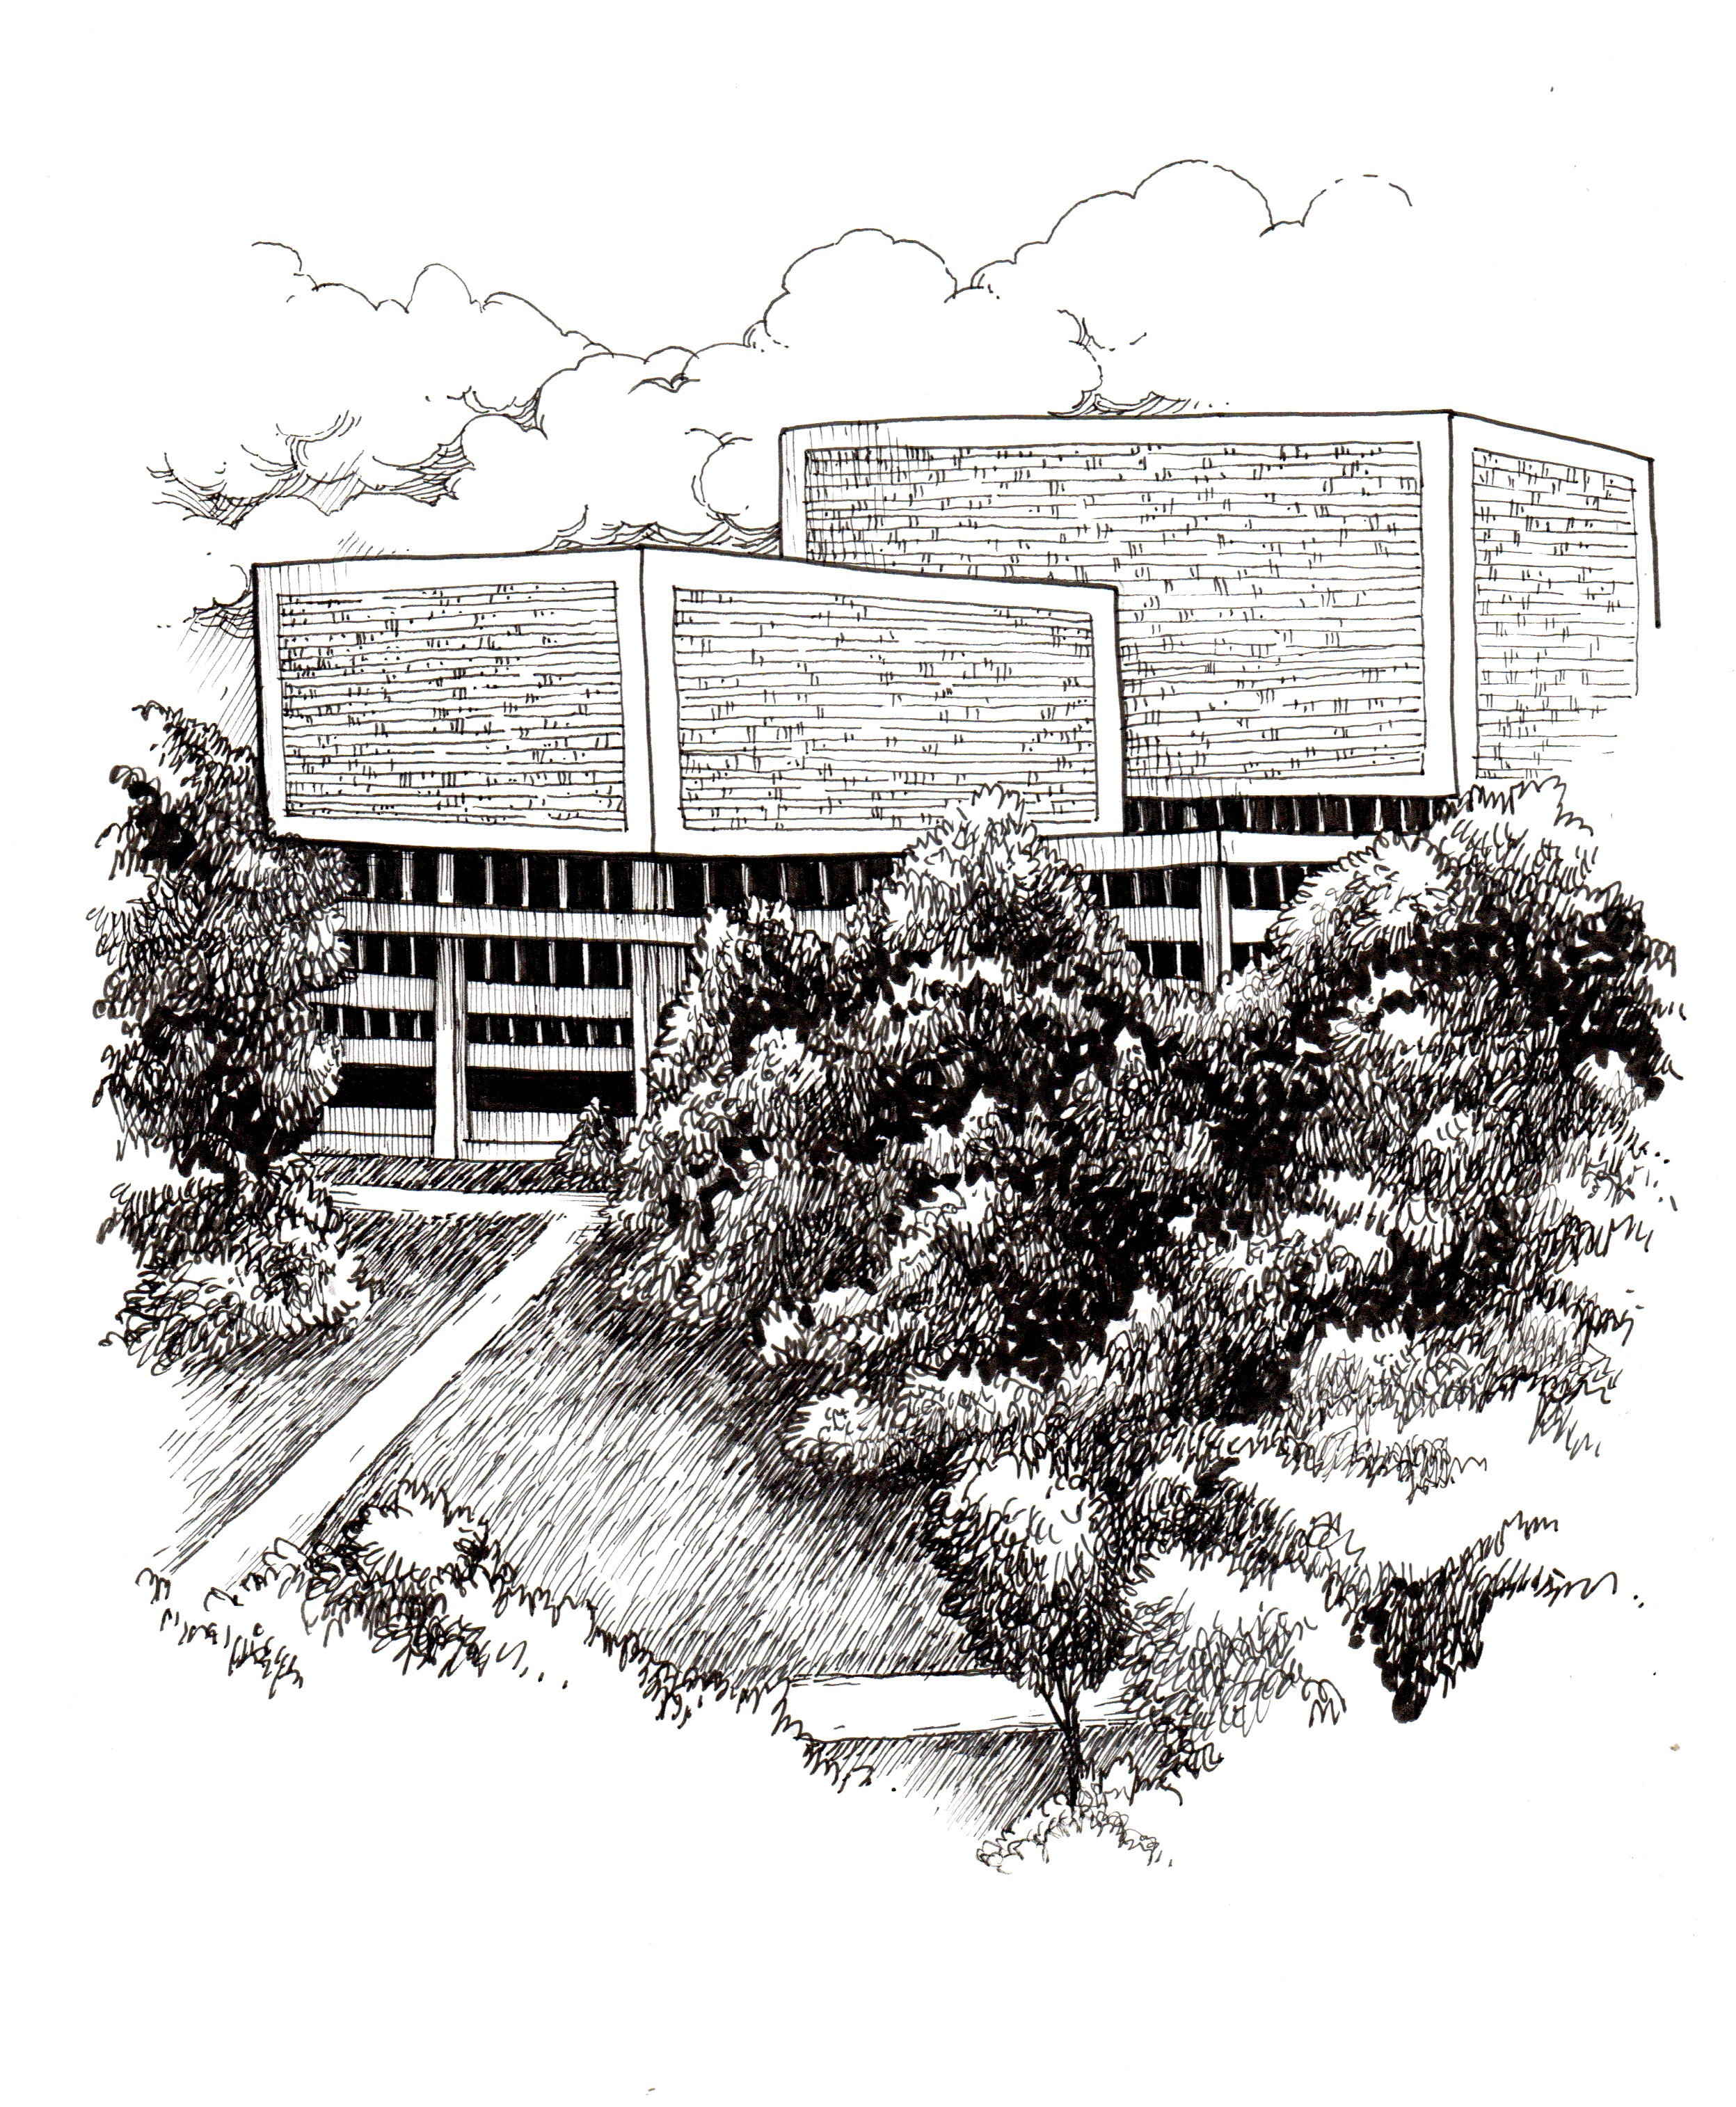
\includegraphics[width=0.6\linewidth,height=\textheight,keepaspectratio]{images/miu6.jpeg}

}

\caption{Herman B Wells Library}

\end{figure}%

\epigraph{
In the United States, the corporate integrity of the university lies in the college idea, as Newman said, which is itself expressed as a territorial entity denominated the "campus." The campus contains the indispensable innumerable symbols and structures: buildings, gardens, bridges, walks, avenues, glades, statues, plazas, fountains, statuary, towers, gateways and also follies, quirky leftover inheritances in the form of inscriptions, unlikely structures and almost unusable ones.  
}
{---Sheldon Rothblatt, ``A Note on the `Integrity' of the University"}

Between 1938 and 1980, Indiana University grew in size, scope, and
stature. The global war that consumed the world from 1939 to 1945
accelerated both the extent and the pace of change, and the postwar
campus that emerged was faithful to the unique design tradition that had
been growing for sixty years. Under the leadership of President Herman
Wells until 1962, the Bloomington campus served a student body that had
increased from five thousand to nearly eighteen thousand when Wells
stepped down. Growth continued, reaching thirty thousand by 1970 and
thirty-five thousand by 1980. To accommodate the growth and
diversification of academic programs, new facilities were added. The
decision to provide ample housing options for students on campus fueled
the construction of an extensive residential life complex, and the
expansion of intercollegiate athletics, both regionally and nationally,
meant the provision of specialized sports facilities.

At the beginning of this period, the campus comprised 137 acres---about
one-fifth of a square mile. By 1968, thirty years later, it had grown
exponentially to encompass nearly the entire northeast quadrant of the
city of Bloomington---about 1,900 acres, or three-square miles. Since
the late 1960s, its size has held steady at 2,000 acres. University
planners had gained a large canvas with which to work, but a large and
enduring challenge faced them: how to knit together the old intimate
precincts surrounding Dunn's Woods with recently acquired ground. As the
cosmopolitan research university emerged, the elemental design mainstays
of trees, stone, and water were employed on a significantly enlarged
campus terrain.

\section{The Campus as a Pedagogical
Agent}\label{the-campus-as-a-pedagogical-agent}

At the close of the Bryan administration in 1937, there were several
major buildings either planned or under construction that would be
finished during the first few years of the Wells regime. They included
buildings for education (now Simon Music Library and Recital Center),
business and economics (now Woodburn Hall), and the physical sciences
(now Swain Hall West). Two dormitories for women, Sycamore Hall and
Beech Hall (now Morrison Hall), completed the Memorial Hall quadrangle
(now Agnes E. Wells Quadrangle); two for men, West Hall (now Edmondson
Hall) and North Hall (now Cravens Hall), completed the Men's Residence
Center (now Collins Living-Learning Center), an open
quadrangle.\footnote{\citeproc{ref-clapacs2017a}{Clapacs, \emph{Indiana
  University Bloomington}, 68--70, 126--31, 172--75, 204--14}.} Finished
in collegiate Gothic style, all were substantial limestone buildings
that fit into established campus districts. The last building
constructed and dedicated before the attack on Pearl Harbor and the
entrance of the United States into the Second World War was the Hall of
Music, more commonly known as the Auditorium.

Within six months of losing his ``acting'' title in 1938, President
Wells recommended to the board of trustees that the architectural firm
of Eggers \& Higgins, from New York City, in collaboration with A. M.
Strauss, a Hoosier architect based in Fort Wayne, be responsible for the
design of a campus auditorium---the Hall of Music---located at the
eastern end of Seventh Street beyond the Men's Gym. Wells was determined
to make his mark on the physical campus by hewing to the established
architectural tradition in the first building planned during his
administration.\footnote{\citeproc{ref-wells1980a}{Wells, \emph{Being
  Lucky}, 198}; \citeproc{ref-capshew2012a}{Capshew, \emph{Herman {B}
  Wells}, 123--25}.}

Excavation began in 1939, but the contractors ran into limestone bedrock
that necessitated additional work. Great shelves of rock and immense
boulders were unearthed. Rather than carry them away for disposal, they
were set aside to create a rock garden immediately north of the
building. This scheme not only saved the cost of disposal but also
enhanced the campus landscape with an artful mimicking of a natural
limestone outcrop. The rock garden, eventually endowed by philanthropist
Elsie Sweeney, joined the Sunken Gardens as another place of beauty
featuring limestone in its natural state.

Pleased with Eggers \& Higgins' work on the Auditorium, in 1940, IU
hired the firm to prepare a feasibility study to add a bowling alley to
the Indiana Memorial Union.\footnote{\citeproc{ref-botm1940a}{Indiana
  University Board of Trustees, {``Minutes of the Board of Trustees of
  Indiana University, 25 March 1940--26 March 1940''} (Bloomington:
  Indiana University Archives \& Indiana University Libraries Digital
  Collections Services, March 25, 1940),
  \url{https://purl.dlib.indiana.edu/iudl/archives/iubot/1940-03-25}}.}
Soon the firm was preparing a site development plan for the entire
campus. ``It was our plan,'' Wells later wrote, ``to try to preserve the
traditional style of architecture on the old campus with as little
modification as possible but, as we moved outward, to allow the
buildings to conform with architectural styles then in
vogue.''\footnote{\citeproc{ref-wells1980a}{Wells, \emph{Being Lucky},
  198}.} That meant, in practice, some limited stylistic experimentation
with collegiate Gothic as well as a few signature buildings in
contemporary modern styles.

Wells lavished care on the planning of a venue that would provide a
superior performance space, whether for musical and dramatic productions
or lectures and convocations. The Auditorium did double duty as the new
permanent gallery for the dramatic murals of Thomas Hart Benton that
were exhibited at the 1933 World's Fair in Chicago.\footnote{\citeproc{ref-capshew2009a}{Capshew,
  {``The Campus as a Pedagogical Agent''}}.} The monumental building
made possible a new design element previously unseen at the Bloomington
campus. Facing west, it was located at the end of Seventh Street atop a
small rise and provided an east-west axis along the street. Starting at
Dunn Meadow, traveling east, on the right was the IMU and on the left
the Men's Gymnasium, and farther, on the right, was the new Business and
Economics Building, with the Auditorium anchoring one end of the axis.
At the request of Wells, Eggers \& Higgins sketched a plan for an open
quadrangle of buildings next to the Auditorium. They produced a scheme
for a building for the fine arts on the north and an open-air
amphitheater on the south slope, near the Jordan River.

In addition, the Wells administration began a relationship with
landscape architect Frits Loonsten in 1940. Based in Indianapolis, the
Dutch-trained Loonsten had a ``great feeling for the natural'' and was
able to figure out ways to seamlessly combine new landscaping with the
old.\footnote{\citeproc{ref-wells1980a}{Wells, \emph{Being Lucky}, 199}.}
As the campus grew, additional green areas were set aside in keeping
with the woodland theme established in the late nineteenth century.

Although classes continued to meet during the war years, mobilization
caused significant changes. Several armed forces training programs used
the campus buildings and grounds, and the academic calendar was
accelerated, with classes year-round and three annual commencements.
Students in military uniforms mingled with civilian undergraduates,
sharing an earnest spirit. Each class from 1940 to 1945 revived the
tradition of funding limestone gates to pierce the low stone walls along
campus boundaries on Third Street and on Indiana Avenue.\footnote{From
  the corner of Third and Indiana, going east along Third Street: 1942,
  1941, 1929, 1926, 1943, 1940; and going north: 1944, 1945.}

As the Second World War was ending, Wells prepared for the predicted
wave of increased enrollments, which would mean increased pressure on
the campus physical plant and facilities. With a banker's foresight, he
directed the treasurer's office to buy contiguous tracts of land from
willing sellers. Between 1944 and 1955, the campus added nearly 1,000
acres to the 140 acres extant at the start of the Wells administration.
Expanding in a northeastward direction, IU now occupied a whole quadrant
of Bloomington, a town of less than thirty thousand.\footnote{US Census
  counts for Bloomington were 20,870 in 1940, 28,163 in 1950, and 31,357
  in 1960.} Sitting on this land-bank, the university had plenty of room
to grow.

\section{Postwar Growth}\label{postwar-growth}

The board of trustees had a nostalgic impulse in 1947 when they
communicated birthday wishes to William Ogg, who had turned ninety-six
on September 12. Every one of the trustees knew Ogg, the former keeper
of grounds from 1899 to 1938, who ``exalted this humble position to make
it one of great importance and inspiration in their lives and in the
lives of countless students and faculty members.'' The board resolved:
``Through fidelity to the task which he loved, through kindness,
friendliness and virtue of his noble life, he enriched the lives of all
of us. He gave flowers for all and their message of beauty and peace
went into the lives of all who trod this campus. He gave us trees, and
many of the oaks planted by his hands stand today straight and strong to
shelter and guide all who come this way. They all symbolized the full
life of this kind and faithful gentleman who served his fellow man in
full measure.''\footnote{\citeproc{ref-botm1947a}{Indiana University
  Board of Trustees, {``Minutes of the Board of Trustees of Indiana
  University, 12 September 1947--13 September 1947''} (Bloomington:
  Indiana University Archives \& Indiana University Libraries Digital
  Collections Services, September 12, 1947),
  \url{https://purl.dlib.indiana.edu/iudl/archives/iubot/1947-09-12}}.}

The unassuming gardener died a year later, a week after his
ninety-seventh birthday. The trustees prepared a memorial resolution,
similar in substance to the birthday wishes given the year before. In
addition to his planting work ``that brightened the lives of those who
took the campus paths, the measure of which service will never be
known,'' Ogg provided a sympathetic ear. As he was working outside, ``he
talked with people in his calm, pleasant and manly way, and many a one
has gone out of his way just to have a chat with Mr.~Ogg, their
friend.''\footnote{\citeproc{ref-botm1948a}{Indiana University Board of
  Trustees, {``Minutes of the Board of Trustees of Indiana University,
  01 October 1948--02 October 1948''}}.}

The postwar world's shape, with its contradictions and opportunities,
was still emerging, but it was already clear it would be different than
the prewar situation. On campus, enrollment doubled in 1946, from 5,000
to 10,000, and a great building program was soon underway. No longer
would the campus revolve around the historic core of Dunn's Woods as
more precincts were developed and activity shifted to new locations. New
academic structures and residence halls and dining facilities claimed
attention among the campus community. The old quadrangle surrounding
Dunn's Woods would remain, still in daily use, but gradually
metamorphizing into a historic landmark.

Student housing was the direst need, and temporary quarters in military
surplus barracks and house trailers were obtained and pressed into
service. For instance, in 1945 a trailer park with three hundred units
was set up on Woodlawn Field, across from the Men's Residence Center,
named Woodlawn Courts. Meanwhile, plans to construct and build a system
of dormitories to the east of the Auditorium were pursued. The first,
Rogers II (now the Ashton Center), was opened in 1945, followed by
several apartment complexes and the Men's Quadrangle (now Wright
Quadrangle) in 1949. They were followed by Smithwood Hall (1955, now
Read Hall), Tower Quadrangle (1959, now Teter Quadrangle), Campus View
Apartments (1962), Foster Quadrangle (1963), McNutt Quadrangle (1964),
Tulip Tree Apartments (1965), Wilkie Residence Center (1965), Forest
Quadrangle (1966), and Eigenmann Hall (1968).\footnote{Clapacs,
  \citeproc{ref-clapacs2017a}{\emph{Indiana University Bloomington}},
  pp.~216--248. See Thomas D. Clark,
  \citeproc{ref-clark1977a}{\emph{Indiana University: Midwestern
  Pioneer: Volume {III}: Years of Fulfillment}, 4 vols. (Bloomington:
  Indiana University Press, 1977)}, p.~197-225}

Military surplus Quonset huts sprang up everywhere, even near the old
quadrangle, to provide needed space for overflowing academic programs.
In 1947, to provide practice and performance space for the School of
Music, the university obtained a surplus airplane hangar from an
Illinois airport and designated East Hall, which included a
one-thousand-seat auditorium, the first home for the opera
program.\footnote{\citeproc{ref-clapacs2017a}{Clapacs, \emph{Indiana
  University Bloomington}, 72--75}; \citeproc{ref-clark1977a}{Clark,
  \emph{Indiana University}, 1977, 485, 498}.} During the postwar
building boom, President Wells ``made a regular tour of construction
sites. He talked with contractors, foremen, workmen, and university
personnel. He climbed through partially constructed buildings, inquired
about schedules, and prayed for good weather, good labor relations, and
speed.''\footnote{\citeproc{ref-clark1977a}{Clark, \emph{Indiana
  University}, 1977, 212}.}

Among the new postwar programs, one depended on campus soil. In 1948,
Assistant Professor of Botany Barbara Shalucha, with the support of her
department and President Wells, started a youth gardening program on
undeveloped campus land on East Tenth Street. Modeled after the Brooklyn
Botanical Garden's program, where Shalucha was previously employed, it
was designed to teach basic horticultural techniques and environmental
science. IU cooperated with the City of Bloomington's Parks and
Recreation Department and the Bloomington Garden Club to provide a
practical outdoor laboratory for area youth.\footnote{\citeproc{ref-bunnage1999a}{JoAnn
  C. Bunnage, {``Barbara Shalucha and the Development of Hilltop Garden
  and Nature Center: The Cultivation of a Community Treasure''} (1999)}.}

In 1961, newly installed lighting in the Well House threatened the
kissing tradition, the \emph{Indiana Daily Student} reported. At
midnight, it seemed as though couples were ``giggling and talking to
each other'' instead of kissing ``in keeping with tradition.'' The
reporter noted, ``The founding fathers located the building away from
campus lights and the beaten path for a purpose\ldots. If the lights
remain, the Well House seems doomed to become nothing more than an
open-air Commons. Coke and candy machines will probably be installed.
This is carrying student enlightenment too far. It is a glaring
error.''\footnote{\citeproc{ref-hunt1961a}{Ralph Hunt, {``Enlightening
  Situation? Well House Wattage Encourages Conversation Rather Than
  Action,''} \emph{Indiana Daily Student}, November 1, 1961}.} This
lighthearted story proved campus usage patterns were changing as the
student body grew and the physical plant increased. Dunn's Woods lost
its centrality after the Second World War as other nodes of campus
activity came into existence serving the needs of an increasingly
cosmopolitan institution.

Another example of the turn away from the old quadrangle occurred in the
early 1960s. The campus, in a vigorous postwar building program, also
looked to existing buildings to address the perennial problem of
creating academic space. But older facilities sometimes suffered under
the bias toward the new. In 1963, Lindley Hall (formerly Science Hall),
built sixty years earlier as the fifth academic hall on the old
quadrangle, was worn and verging on decrepit. The president and the
trustees identified Lindley Hall as a possible candidate for replacement
in a structural review.\footnote{\citeproc{ref-botm1963a}{Indiana
  University Board of Trustees, {``Minutes of the Board of Trustees of
  Indiana University, 31 May 1963--03 June 1963''} (Bloomington: Indiana
  University Archives \& Indiana University Libraries Digital
  Collections Services, May 31, 1963),
  \url{https://purl.dlib.indiana.edu/iudl/archives/iubot/1963-05-31}}.}
The review indicated that the building was not so severely dilapidated
that it would make sense to tear it down, so some modest repairs and
improvements were approved. Looking back, this decision upheld the
design integrity of the original quadrangle, thus ``avoiding the mistake
of many other universities that destroyed their architectural
legacies.''\footnote{\citeproc{ref-clapacs2017a}{Clapacs, \emph{Indiana
  University Bloomington}, 40}.}

\section{Tying the Present to the
Past}\label{tying-the-present-to-the-past}

Amid the postwar transformation of the campus to serve a great expansion
of IU's mission of education, research, and service, a faculty member
reflected on the role of trees in shaping the design of the physical
plant. In 1960, botany professor emeritus Paul Weatherwax published a
short article, ``Familiar Trees Greet Returning Alumni,'' in \emph{The
Review}, a publication for arts and sciences alumni. A specialist on the
evolution of the corn plant, Weatherwax received both his undergraduate
and graduate degrees from IU and started teaching in 1918. Well
acquainted with fellow botany professor David Mottier, he shared an
appreciation for the southern Indiana landscape. His article empathizes
with returning alumni: ``New buildings everywhere, old buildings with
new names, new walks and drives, and memories of old thoroughfares which
can no longer be found, all add up to a bewildering picture of growth
and change.'' But campus trees ``turn out to be faithful old
landmarks''---``something to tie the present to the past.''

The article went on to briefly recount the history of campus design,
focusing on the role and care of trees, including tree surgery.
Naturally, the botanist included some comments on tree identification.
Countering the common misperception that every kind of tree that grew in
Indiana was to be found on the campus and that there were hundreds and
hundreds of them, Weatherwax stated that there were fewer than 150
species across the Hoosier state and perhaps fewer than seventy to be
found on the campus. He went on a verbal tour around campus, pointing
out a dozen or so species, including beech, sugar maple, oak, sycamore,
tulip poplar, tamarack, bald cypress, ginkgo, and pine. He gently
exhorted, ``To live among the trees without knowing anything about them
is much like living in a foreign country among people whose names you do
not know and whose language you do not understand\ldots. The time and
effort invested in learning something about the trees and other natural
things in our environment will yield generous dividends for a
lifetime.''\footnote{\citeproc{ref-weatherwax1960a}{Paul Weatherwax,
  {``Familiar Trees Greet Returning Alumni,''} \emph{The Review}, May
  1960, 12--18}.} Weatherwax's article caught the eye of President
Wells, a fellow tree-lover.

In 1961, in his last year as president, Wells wrote a two-page letter to
Weatherwax urging him to expand the article into a pamphlet ``to
enlighten incoming freshmen about the design history of their campus and
to promote this legacy to visitors and alumni.'' He went into some
detail, eleven points in all, about the proposed content. Wells thought
it would be ``a very great contribution to the building of affection for
our Alma Mater.'' Ending the letter with ``one final thought---put in a
ringing warning against any plan to put buildings in the wooded areas,''
Wells reaffirmed yet again the administrative commitment to preserve and
protect the trees.\footnote{\citeproc{ref-wells1961a}{Herman B. Wells,
  {``Letter to Paul Weatherwax''} (Lilly institution/LMC 2283/B4/F
  Wells, Herman B., August 22, 1961)}.}

Weatherwax took Wells's suggestion and revised the text into a booklet,
\emph{The Woodland Campus of Indiana University}, first published in
1966. More than a guide for tree identification, it was a testimonial to
the campus design path that the university had taken over the previous
seventy-five years and was designed to inspire pride in the aesthetic
qualities of the contemporary campus. Enlivened with anecdotes and
historical tidbits, about half the content concerned tree
identification, aided by a map for a self-guided tour of the sylvan
beauty of the campus.

Wells, the university chancellor since 1962, provided an introduction in
the form of a letter ``to the students of Indiana University.''
Proclaiming ``we share a priceless heritage,'' he wrote, ``Our campus is
unique and beautiful. It is unique because it preserves areas of forest,
maintained in as near natural state as daily use by thousands of us will
permit.'' Wells wrote of the beauty revealed through each season and the
need for ``breathing space'' in the face of increasing urbanization.
Paying tribute to earlier conservationists, he stated, ``To cut a tree
unnecessarily has long been an act of treason against our heritage and
the loyalty, love, and effort of our predecessors who have preserved it
for us.'' After a paragraph explaining the mission of the IU Foundation,
he suggests: ``Our forest trees are your link to the past. The Indiana
University Foundation is your link to the future.'' Wells, paraphrasing
an earlier speech, hoped, ``May you find on the campus, especially the
old quadrangle, the beauty and sanctuary which will inspire you to dream
long dreams of future usefulness to society.''\footnote{\citeproc{ref-weatherwax1966a}{Paul
  Weatherwax, \emph{The Woodland Campus of Indiana University}
  (Bloomington: Indiana University, 1966), 2--3}.}

In the main text, Weatherwax invited the reader ``to pause occasionally
and appreciate this unusual beauty which has been enjoyed for many
generations which of those who have preceded you,'' adding the hope that
support to ``preserve this heritage'' will result. After a brief
discussion of the old seminary campus and the move to Dunn's Woods,
Weatherwax highlighted various groundskeepers, including William Ogg,
along with faculty members David Mottier and J. Van Hook, as key figures
in the creation of the woodland campus. Weatherwax dryly noted that the
``removal of a tree for any reason has always been a fighting matter,
with emotion often pitted against sound judgement.'' He explained, ``In
spite of misguided protests, better judgement generally prevailed, and
the campus developed by a series of compromises.''\footnote{\citeproc{ref-weatherwax1966a}{Weatherwax,
  5--7}.}

Moving to open space planning, Weatherwax talked about the lands east of
Jordan Avenue, where residential halls were being constructed amid
wartime surplus buildings serving as temporary dormitories. The
makeshift structures, each named after a native tree (e.g., Pine Hall)
and known collectively as Trees Center, were to be removed, and
afterward, ``it is hoped that it will revert to the original forested
state.'' Despite strong pressures to further develop open land for
practical uses in the future, ``these spots of natural beauty on the
campus, our most stable link with our pioneer past, must be preserved
for future generation,'' Weatherwax maintained.\footnote{\citeproc{ref-weatherwax1966a}{Weatherwax,
  12}.}

Turning from politics to botany, Weatherwax admitted that ``trees on a
college campus have, at best, a hard time of it,'' as they face a host
of environmental challenges caused by the man-made hardscape even though
they receive dedicated care. ``Effort is made to steer a sensible course
between what is best for the trees and what use is to be made of the
campus.'' The basic biology of trees and their life cycles were
presented, and the roles of native wildflowers and animals were also
mentioned. A list of nearly one hundred ``trees you may wish to
recognize'' was followed by a map of the older parts of campus that
noted the locations of sixty species. About half of the booklet was
devoted to the campus tree guide, describing both common and unusual
species found on the campus.\footnote{\citeproc{ref-weatherwax1966a}{Weatherwax,
  13--28}.}

With its pedagogic aims of environmental education coupled with an
appreciation of the natural landscape, the booklet had wide appeal and
addressed many interests---historical, artistic, ecological,
philanthropic, recreational, as well as educational. Waxing poetic,
Weatherwax summed up the main point: ``There are few places in the world
where great laboratories, classrooms, libraries, and other centers of
intellectual and artistic activity are located in an environment which
retains its primeval character---few places where one may so quickly go
to shed the tensions and anxieties of this complex modern world in quiet
meditation.''

He added a challenge: ``Are we so poor that we cannot afford to preserve
this precious heritage? Indeed, are we so rich that we can afford to
lose it?''\footnote{\citeproc{ref-weatherwax1966a}{Weatherwax, 17}.} The
pamphlet went through several revisions and republications in the years
following.

\emph{The Woodland Campus of Indiana University} considered the campus
worthy of consideration, over and apart from its daily functioning, for
a myriad of educational activities. Campus design was explicitly
connected to pedagogical purposes, and knowing the history of a basic
natural feature---trees---was deemed valuable. Among the important
messages conveyed by this publication was that students learn from the
environment surrounding them, both indoors and outside.

The booklet was published when the presidential administration of Elvis
J. Stahr was well underway. His administration, lasting from 1962 to
1968, saw the conclusion of a major building program at the Bloomington
campus that stretched back to the 1930s. As the rate of enrollment
increase began to slow, the commitment to house a sizable portion of
students on campus neared completion. The main campus reached nearly
2,000 acres---its present size. Of the dozen major buildings and
facilities completed during his tenure, seven were housing for students
and three were for academic departments.\footnote{Student housing:
  Foster, McNutt, Briscoe, Tulip Tree, Willkie, Forest, and Eigenmann;
  academic structures for psychology, radio and television, and
  business. See Clapacs, \citeproc{ref-clapacs2017a}{\emph{Indiana
  University Bloomington}}, p.~470. In 1966, a faculty Committee on
  Natural Areas proposed a preliminary plan for University Woods,
  encompassing the shore of Griffy Reservoir and the University Lake
  area, for further development of research and teaching. See J. A.
  Franklin, \citeproc{ref-franklin1966a}{{``Letter to Thomas {D}.
  Brock''} (Indiana University Archives/C268/B13/F Committee, Natural
  Areas, July 21, 1966)}.}

Beyond Bloomington, there was a surge of construction at the IU
Extension Centers located around the state, as the university underlined
its educational commitment to regional hubs through bricks or limestone
and mortar. In 1968, the centers gained more autonomy and were
designated regional campuses.\footnote{For basic information on the
  history of the regional campuses, see
  \href{https://expand.iu.edu/browse/iuheritage/courses/iu-history-campuses-context}{IU
  History: Campuses \& Context}}

\section{Earth Day 1970}\label{earth-day-1970}

The startling view of ``Earthrise'' taken from the Apollo 8 mission to
the moon on December 24, 1968, was breathtaking. It offered a new
perspective of our planetary home as a beautiful gem in the vastness of
space. The idea of ``Spaceship Earth,'' given concrete form by the
Apollo photographs, presaged the awakening provided by Earth Day in
1970.

As the 1960s wore on, groups of people in various parts of the country
focused on problems of pollution of the environment. Toxic emissions
from industries and automobiles befouling the air, poisonous waste
dumped in rivers and lakes, landfills leaching chemicals into the water
table, dangerous insecticides and herbicides, oil spills along the
coast, and the ``tragedy of the commons'' were debated. The words
\emph{ecology} and \emph{environment} started to pepper public
discourse. Among the national voices were several IU faculty, Elinor
Ostrom, Vincent Ostrom, and Lynton Caldwell among them.

Wisconsin senator Gaylord Nelson, aware of these emerging issues,
devised a way to increase public consciousness about the fraying of the
nation's ecological fabric: a civic demonstration expressing care of the
Earth, first thought of as an environmental ``teach-in'' and then as an
``environmental action day.'' The senator wisely let planning staff
groups from universities, colleges, cities, and towns across the United
States plan locally relevant programs. At Indiana University, an
organization emerged with the name Crisis Biology to serve as a
clearinghouse for Earth Day and related plans. Associate Professor of
Botany Donald Whitehead served as chair of the steering committee for
Environmental Action Day.\footnote{\citeproc{ref-schlechtweg1970a}{Harold
  Schlechtweg, {``Environmental Day Activities Listed,''} \emph{Indiana
  Daily Student}, April 20, 1970}.}

The schedule of activities for the first Earth Day on April 22, 1970,
was impressively extensive. Dunn Meadow, the site of numerous music
concerts and protest demonstrations in the past, was chosen as the site.
Bob Scott, a junior, summed up the attraction in the student newspaper;
``The Revolution Is Here, Escape in Dunn Meadow'' was the headline:

\begin{quote}
It is the communal ground and ancestral home for the young. It is I.U.'s
continuing Woodstock. In Dunn Meadow, people run wild and go crazy in
the spring, in all of the good weather and some of the bad. In Dunn
Meadow there is no saturating up-tightness, only the warmth that comes
from the closeness of the earth, the blueness of the sky, and the
oneness of people being happy. We all want to escape to a Dunn Meadow of
the mind\ldots. Dunn Meadow is the spirit of freedom.\footnote{\citeproc{ref-scott1970a}{Bob
  Scott, {``The Revolution Is Here, Escape in Dunn Meadow,''}
  \emph{Indiana Daily Student}, April 20, 1970}.}
\end{quote}

The meadow, acting as the expansive side yard of the Indiana Memorial
Union, could handle the large crowd expected.

The organizers scored a coup in attracting Senator Nelson to open the
festivities with an address. It was the start of a long two days for
him, with speaking engagements in Madison, Milwaukee, Boston, Atlanta,
Denver, and Berkeley as well. Bloomington was the smallest metro area on
his itinerary.\footnote{\citeproc{ref-bischoff1970a}{Sue Bischoff,
  {``Nelson Pleased by Turnout, Originality,''} \emph{Indiana Daily
  Student}, n.d.}} Around 2,000 people attended Nelson's 9:30 a.m.
address. Righteous cries of ``Right on!'' punctuated the air. Pollution,
he declared, was the most important issue facing humanity. Briefly
interrupting Nelson's speech, about ten women dressed as witches
performed some guerrilla theater, dancing in a circle and chanting,
``Save our bodies, save ourselves,'' demonstrating for the free use of
contraceptive devices and against abortion laws. Returning to his
remarks, Nelson said the problem of pollution had two aspects, the
philosophical and the physical. To counteract the ideology that humans
are ``over, above, and separate from the rest of nature,'' he called for
changes in ``philosophical beliefs, feelings, and attitudes toward
nature.'' On the physical side, Nelson wanted remedial actions to take
place on the national level in addition to state and local efforts.

On the podium with Nelson was Robert Menke, an IU trustee. He reminded
the crowd that ``the concern of past leaders of the environment'' was
demonstrated by IU's beautiful campus. ``I have faith in the future,''
Menke declared, ``because I have faith in the young people of
America.''\footnote{\citeproc{ref-schlechtweg1970b}{Harold Schlechtweg,
  {``Nelson Outlines Proposals to End National Pollution,''}
  \emph{Indiana Daily Student}, April 23, 1970}.}

After the speeches by Nelson and Menke, the Environmental Fair opened.
People were free to visit tables and booths set up in Dunn Meadow where
groups with connections to the environment had displays and information.
``Their subject matter ranged from Planned Parenthood to organic food;
from non-detergent soap to a soft drink company's use of reusable
bottles,'' \emph{Indiana Daily Student} reporters observed, adding,
``The sophistication of the exhibits ran the gamut from grade school
level crayon posters to a scale model farm pond---complete with fish and
frog.''\footnote{\citeproc{ref-ferries1970a}{Ken Ferries and Linda
  Herman, {``{Woodstock, 4-H Flavor I.U. Environmental Fair},''}
  \emph{Indiana Daily Student}, April 23, 1970}.} Rock music accompanied
the Environmental Fair all day, with local favorite bands the Screaming
Gypsies, Pure Funk, and others providing the soundtrack. Adults and
young people, parents and children all intermingled---wandering,
dancing, playing Frisbee, wading in the Jordan River (``one of the
campus' primary pollution symbols,'' the reporter noted). Random
guerrilla theater continued. Booth workers engaged people in
conversation and passed out information. Some, like IU sophomore Steve
Gudeman, worried about the intent of the buoyant crowd: ``I'm afraid
they really aren't serious. I'm interested in seeing how much work is
done by the committees after this.'' The \emph{IDS} summarized the
action at the Environmental Fair: ``Beneath a sky that never quite had
the heart to rain, I.U. played out its bit of Earth Day. The
`ceremonies' were a stew of Indiana `4-H' with a strong dash of
Woodstock thrown in for flavor.''\footnote{\citeproc{ref-ferries1970a}{Ferries
  and Herman}.} Echoing recent protests against the Vietnam War and
massive tuition increases, Dunn Meadow was the setting for a new type of
demonstration on behalf of the environment.

In keeping with the eclectic and polycentric day, there was a wealth of
other activities. There were ``pollution tours'' of Bloomington by bus.
There was an all-day Environmental Film Program, sponsored by the IU
Audio-Visual Center, in Whittenberger Auditorium. Environmental justice
themes were the focus of film and discussion: ``The Environment and the
Poor: Someone Pays the Price.'' A multidisciplinary mini-symposium with
IU professors explored ``Alternatives to Present Urban
Trends.''\footnote{The speakers were professors Frederick Churchill,
  Lloyd Orr, George Smerk, and Al Ruesink.} The Interfraternity Council
organized the SMUT (Students March Upon Trash) campaign as a campus
cleanup. Residence halls and Greek houses, twenty-five in all, had
multiple speakers on environmental topics. At night, WTIU broadcast a
televised panel discussion (with a simultaneous radio broadcast on
WFIU), ``Environmental Action Day: A Beginning,'' with local and state
government officials and interested citizens to assess existing problems
and prospects for the future.\footnote{\citeproc{ref-ids1970a}{{``Environmental
  Action Day April 22 Schedule of Activities,''} \emph{Indiana Daily
  Student}, April 22, 1970}.}

Featuring other national figures, an evening symposium in the IU
Auditorium closed Earth Day. Entitled ``Environmental Action: It's Up to
Us,'' the symposium was moderated by botany professor and chair of the
Earth Day committee Donald Whitehead. The speakers included Leon
Billings, chief of staff to Senator Edmund Muskie and staff director of
the US Senate Subcommittee on Air and Water Pollution, and US
Representative Lee Hamilton, representing the ninth congressional
district since 1965.\footnote{Billings was a major architect of the
  Clean Air Act, signed by President Nixon on December 31, 1970. See
  also Sam Roberts, \citeproc{ref-roberts2016a}{{``Leon {G}. Billings,
  Architect of Clean Air and Clean Water Acts, Dies at 78,''} \emph{New
  York Times}, November 17, 2016}.} Back on campus was former IU
president Elvis Stahr, two years after he stepped down and assumed the
presidency of the National Audubon Society, revitalizing the venerable
bird-watching organization into an activist environmental
watchdog.\footnote{\citeproc{ref-schlechtweg1970a}{Schlechtweg,
  {``Environmental Day Activities Listed''}}.}

Representative Hamilton began, ``With astounding alacrity, we have all
become environmentalists,'' adding, ``The environment is a politician's
delight'' because ``everyone is for clean air, clear water, and tall
forests.'' But he injected a note of caution: ``In spite of all the
protests, meetings, commissions, speeches, legislation, organizations,
in spite even of the enormous political popularity of the issue, I am
not fully persuaded that we have begun to grasp the dimensions of the
environmental task.'' Hamilton went on to say that we must clearly see
the complexities of the task of cleaning up the environment and warned
about the dangers of single-minded thinking and of assigning blame to
others. ``The fact is,'' he declared, ``that all of us are polluters and
all living Americans are big polluters.'' He spoke of power politics and
the voices of industry and business and the trade-offs that are
involved: ``Pollution control may mean short term competitive
disadvantage.'' In his view, management of the environment is above all
a political issue, and ``politics, not science, is the key to whether or
not we succeed.''

Hamilton saw problems in the proliferation of governmental groups
dealing with the environment---``11 federal departments, 16 independent
agencies, 13 congressional committees, 90 federal programs, 26
quasi-governmental bodies, and 14 interagency committees''---with hope
that the planned establishment of the Environmental Protection Agency
would begin to rationalize the system of federal oversight. Moving to
individual lifestyle choices, he suggested giving up so-called
``luxury'' if that means ``squandering and spoiling resources.''
Hamilton reviewed pending federal legislation concerning the environment
and some state initiatives, noting that Indiana would spend 1.9¢ per
person in the biennium for air pollution control, in contrast to
Kentucky, where 10.4¢ would be expended. He concluded his speech with a
lengthy list of steps for everyone to take, dealing with community
engagement on a variety of environmental issues. ``When the hoopla and
the shouting die, the flags no longer wave, and Earth Day has come and
gone, our task will be to persevere. So join the fray---if you don't,
who will?''\footnote{\citeproc{ref-hamilton1970a}{Lee Hamilton, {``The
  Popularity of the Environmental Issue''} (Indiana University
  Archives/Lee H. Hamilton Congressional Papers,
  1965--1998/MPP2B142/Folder 18, Speech Book 16, Q., April 22, 1970)}.}

Earth Day was a symptom of a rising tide of environmental consciousness
that was sweeping the nation. Congress had just passed the National
Environmental Policy Act in 1969 to ``create and maintain conditions
under which man and nature can exist in productive harmony'' and to
``assure for all Americans safe, healthful, productive, esthetically and
culturally pleasing surroundings.''\footnote{\citeproc{ref-epa1992a}{{``The
  Guardian: Origins of the EPA,''} \emph{EPA Historical Publication-1},
  Spring 1992}.} It contained an innovative tool of analysis of likely
consequences---the ``Environmental Impact Statement''---that all federal
projects were required to submit. A new federal institution, the
Environmental Protection Agency, was formed in 1970, cobbled together
from existing departments and bureaus and designed to rationalize
pollution control and establish environmental baselines.

At Indiana University, faculty members were contributing to the national
discussion as well as creating new academic frameworks to sustain
research, teaching, and service in this arena. Lynton Caldwell, a
political science professor, was credited with drafting the text of the
1969 National Environmental Policy Act in collaboration with Senator
Henry Jackson's office. Earlier, in 1963, Caldwell wrote a
groundbreaking article, ``Environment: A New Focus for Public Policy?''
that helped launch a new subfield.\footnote{\citeproc{ref-caldwell1963a}{Lynton
  K. Caldwell, {``Environment: A New Focus for Public Policy?''}
  \emph{Public Administration Review} 23 (1963): 132--39}.} On the IU
campus, Caldwell and others advocated for the formation of a new
school---School of Public and Environmental Affairs---which was created
in 1972. Known by its acronym, SPEA was an unusual hybrid, with public
policy studies coexisting alongside environmental science programs, with
aspirations of cross-fertilization. With the concentration on national
and international issues, there was less focus on local environmental
issues, although that would slowly change. SPEA, a robust response to
emerging issues of concern in modern life, was the first new
professional school established at IU in decades. Much of the
organizational framework for professional schools had been put in place
in the 1920s and had served well since then.

A new presidential administration began in 1971, when the vice president
for regional campuses, John W. Ryan, was selected by the board of
trustees to serve. An IU Ph.D.~alumnus in political science, Ryan was in
office for sixteen years, until 1987. His administration supervised the
construction of several landmark structures that rounded out the
physical plant. In 1971, the Musical Arts Center, perhaps the finest
opera house on a college campus in the nation, was completed, as was
Assembly Hall (now Simon Skjodt Assembly Hall) to provide a venue to
showcase IU basketball. Ten years later, the IU Art Museum (now the
Eskenazi Museum of Art), with a ``starchitect'' building by I. M. Pei,
complemented the Fine Arts Plaza, and the new Bill Armstrong Stadium
provided a field for the IU soccer teams as well as a track for Little
500 cycling races.

In 1980, the original campus at Dunn's Woods, including nine historic
buildings on the old quadrangle and the remnant woodland, was listed on
the National Register of Historic Places. The listing was a local
outgrowth of historic preservation awareness and initiatives that
stemmed from the 1976 national bicentennial. The nomination packet of
text and pictures referred to these historic buildings collectively as
the ``Old Crescent,'' certainly an evocative appellation, albeit
completely new. This coinage rounded off the corners of the old
quadrangle, bundled the buildings together, and inscribed a venerable
label for a historic precinct. ``Old Crescent'' caught on quickly,
unlike ``University Park'' nearly a century earlier.\footnote{I have not
  found any references to ``Old Crescent'' relating to the IUB campus
  until after the NRHP designation. The nomination form was prepared by
  Daniel F. Harrington, c/o Indiana Geological Survey, on behalf of the
  Indiana University Heritage Committee. The ``Name'' box had ``historic
  and/or common''; ``The Old Crescent'' was listed as the common name.
  \citeproc{ref-hcrs1980a}{{``The Old Crescent''} (NRHP
  Inventory-Nomination Form; United States Department of the Interior:
  Heritage Conservation and Recreation Service, 1980)}.}

\bookmarksetup{startatroot}

\chapter{Landscapes of Learning}\label{sec-seven}

\begin{figure}[H]

{\centering 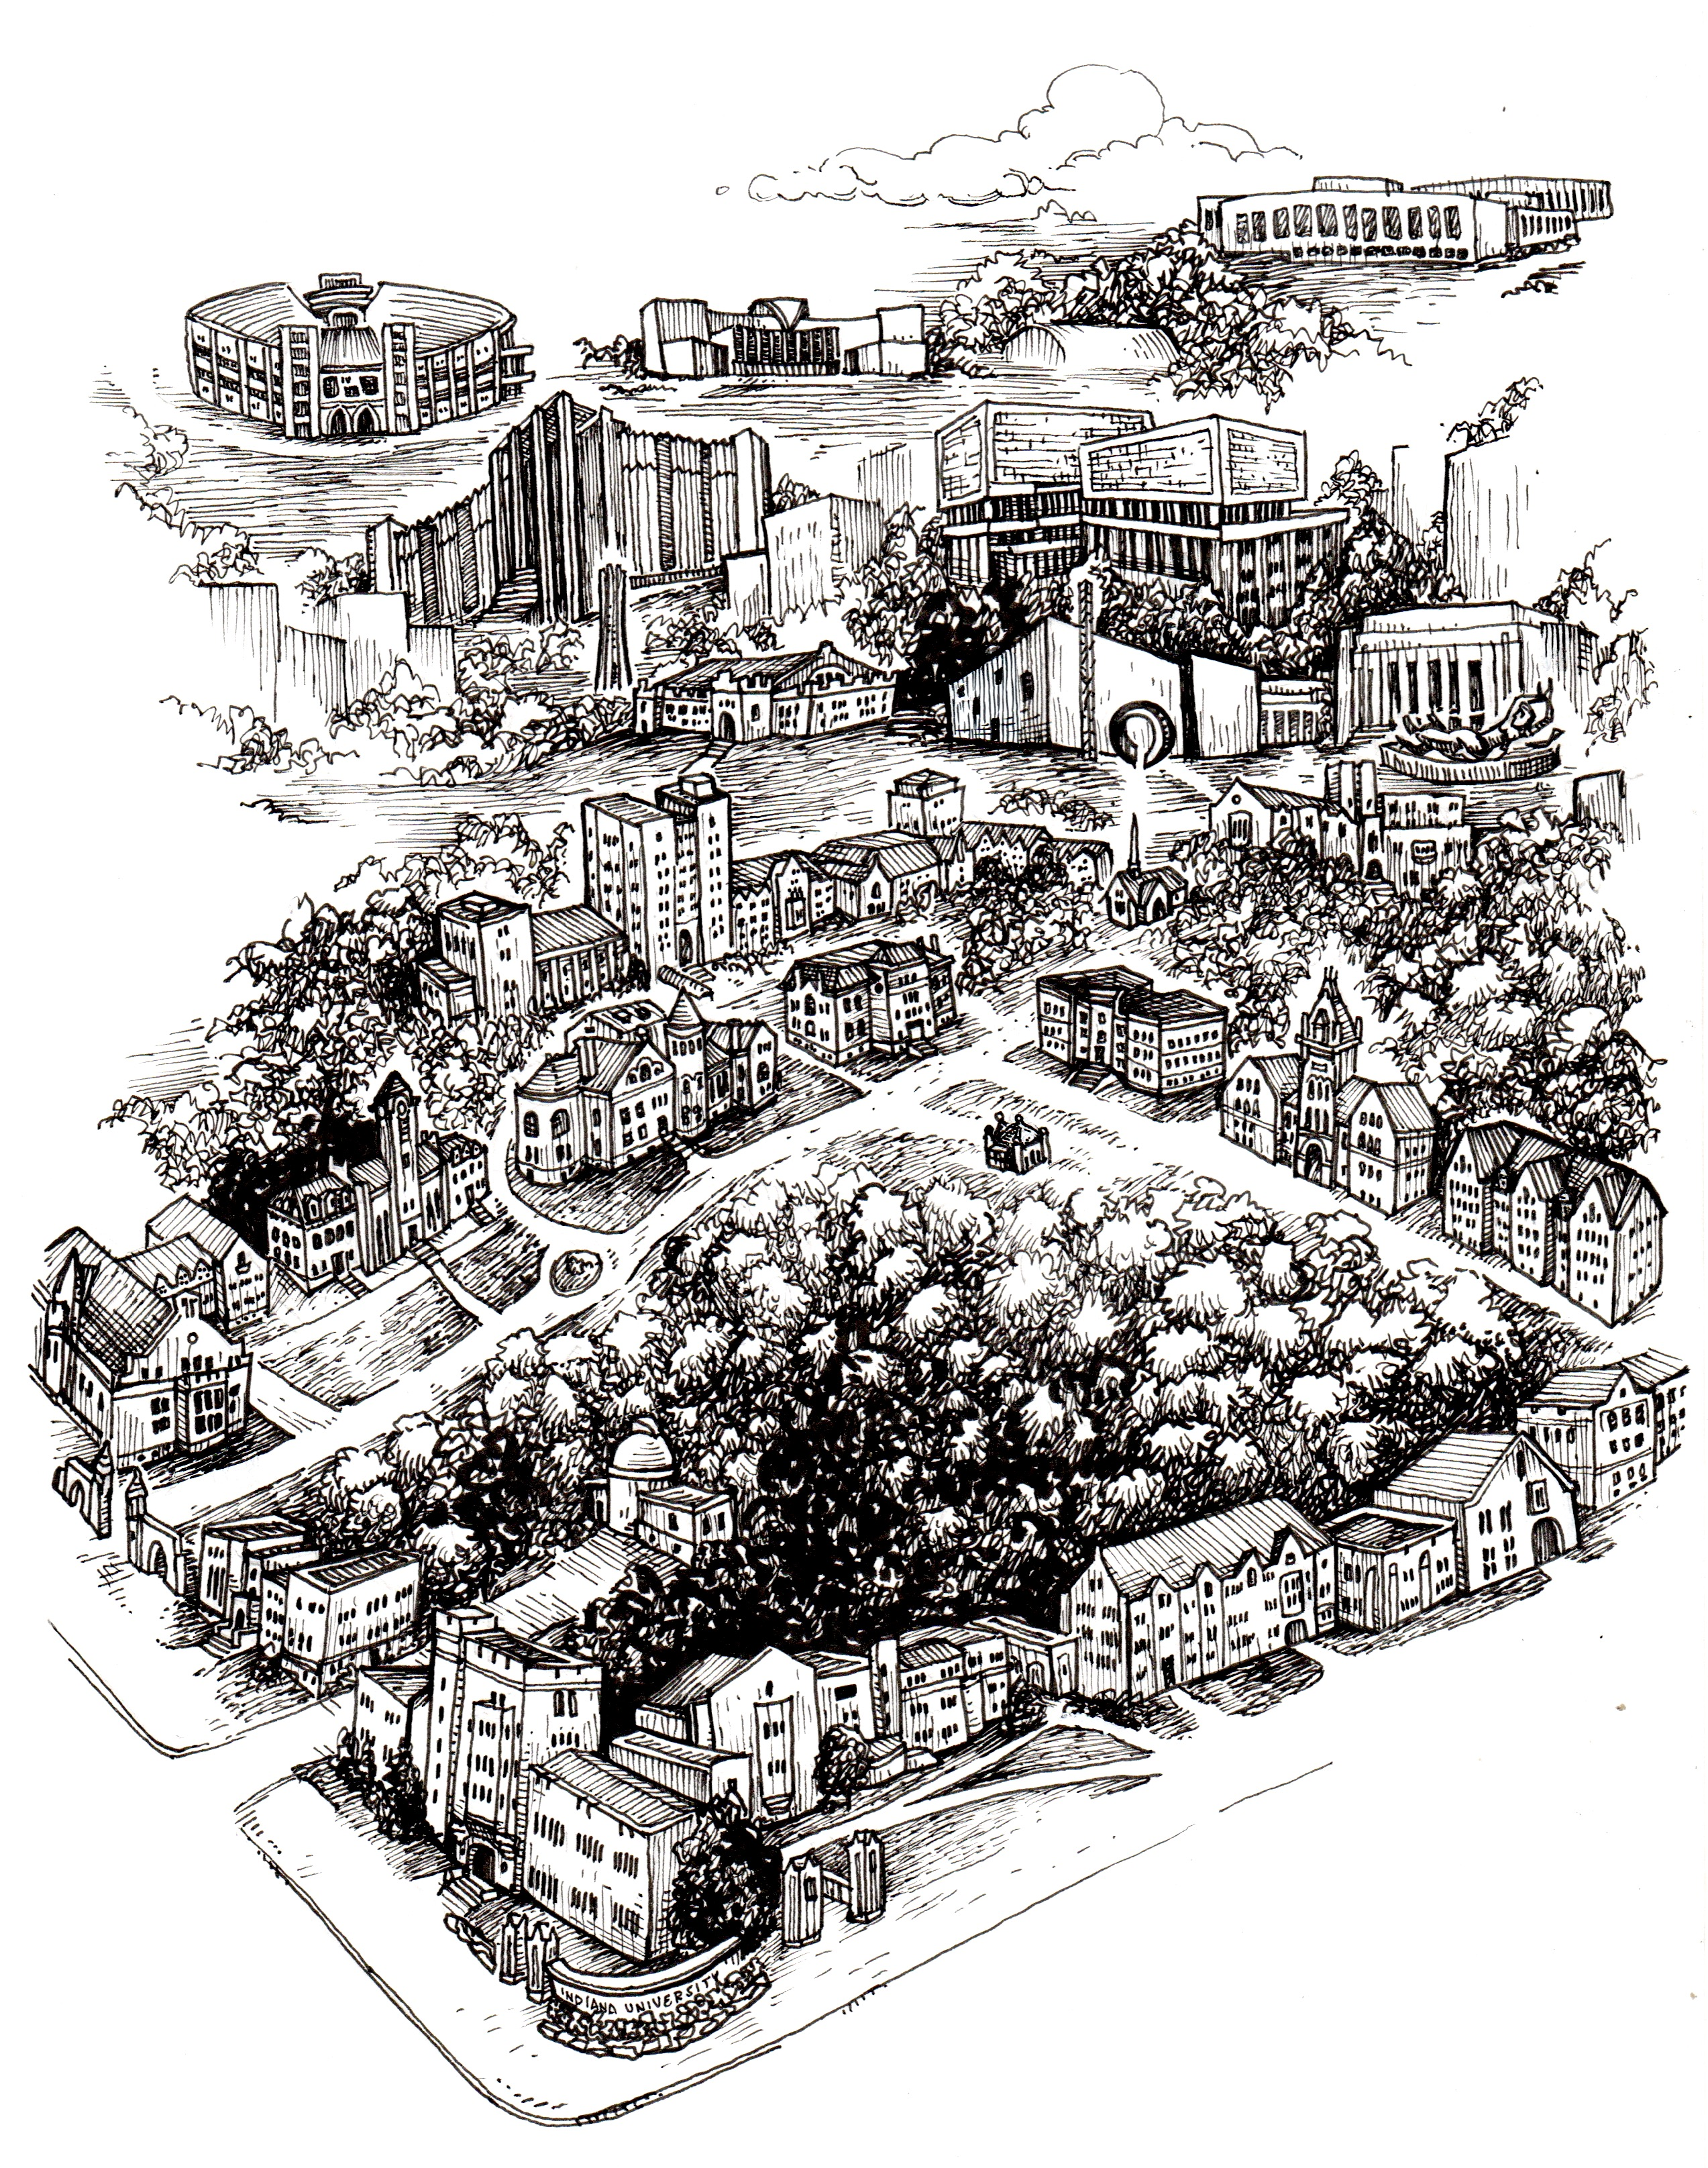
\includegraphics[width=0.6\linewidth,height=\textheight,keepaspectratio]{images/miu7.jpeg}

}

\caption{IU Bloomington Campus}

\end{figure}%

\epigraph{
We know that the campus itself must be the teacher, a place that gives vitality, meaning, and memory to the learning experience, not just within the confines of the institution but in the times and places beyond. I have argued that those are the fundamental attributes of the place-based institution---its soul, if you please---that have enabled it to persevere throughout our restless history, to continuously transform itself as it has tackled the ever-changing needs of American society.  
}
{---M. Perry Chapman, \textit{American Places: In Search of the Twenty-First Century Campus}}

The flagship Indiana University campus one sees today is but the latest
culmination of a partnership between humans and nonhuman nature that
began in 1885. The environmental history of the IU Bloomington (IUB)
campus between 1980 and 2020 was shaped by a shared understanding of the
importance of the woodland theme in campus design that emerged in the
1880s and its successful adaptation to post--World War II circumstances.
Presidents John Ryan (1971--87), Tom Ehrlich (1987--94), Myles Brand
(1994--2002), Adam Herbert (2003--07), and Michael McRobbie (2007--21)
continued this remarkable continuity of vision and practice while their
administrations served as stewards of the campus design ethos. But
leadership was only one part of the equation. Faculty, staff, students,
alumni, and Bloomington townspeople shaped the campus with their actions
and care, as did architects, contractors, and gardeners who brought
plans and blueprints to life.

Relabeling the Dunn's Woods quadrangle of buildings as the Old Crescent
in 1980 served to differentiate the historic core from newer areas on
the sprawling campus. But the challenges to integrating academics,
residential life, and athletics within the physical plant continued.
Construction persisted, with a mix of new buildings, renovations of
older structures, and, occasionally, wholesale redevelopment. In this
period, university officials occasionally faced organized local public
opposition to proposed land use decisions and facility planning,
sometimes leading to the modification or abandonment of design schemes.

\section{Law School Addition}\label{law-school-addition}

The School of Law building, located at Indiana Avenue and Third Street
since 1957, anchored the southwest corner of the historic campus
quadrangle. Concern over maintaining accreditation standards led to
plans to expand and renovate the law library, and the Ryan
administration negotiated with the Phi Gamma Delta (Fijis) fraternity
next door to buy their property. After talks collapsed in the fall of
1981, the board of trustees approved the construction of an addition on
the back of the existing law building.\footnote{An addition had been
  discussed for years, and the trustees had hired architects in 1980 to
  prepare plans. IU had sought bonding authority for the \$11 million
  project, but the state budget bill reduced the amount to \$5 million
  in spring 1981. Indiana University Board of Trustees,
  \citeproc{ref-botm1980a}{{``Minutes of the Board of Trustees of
  Indiana University, 02 February 1980''} (Bloomington: Indiana
  University Archives \& Indiana University Libraries Digital
  Collections Services, February 2, 1980),
  \url{https://purl.dlib.indiana.edu/iudl/archives/iubot/1980-02-02}};
  Indiana University Board of Trustees,
  \citeproc{ref-botm1980b}{{``Minutes of the Board of Trustees of
  Indiana University, 09 May 1980''} (Bloomington: Indiana University
  Archives \& Indiana University Libraries Digital Collections Services,
  May 9, 1980),
  \url{https://purl.dlib.indiana.edu/iudl/archives/iubot/1980-05-09}};
  Indiana University Board of Trustees,
  \citeproc{ref-botm1981a}{{``Minutes of the Board of Trustees of
  Indiana University, 03 March 1981''} (Bloomington: Indiana University
  Archives \& Indiana University Libraries Digital Collections Services,
  March 7, 1980),
  \url{https://purl.dlib.indiana.edu/iudl/archives/iubot/1981-03-07}};
  Indiana University Board of Trustees,
  \citeproc{ref-botm1981b}{{``Minutes of the Board of Trustees of
  Indiana University, 05 December 1981''} (Bloomington: Indiana
  University Archives \& Indiana University Libraries Digital
  Collections Services, December 5, 1980),
  \url{https://purl.dlib.indiana.edu/iudl/archives/iubot/1981-12-05}};
  and John Fancher, \citeproc{ref-fancher1981a}{{``IU Trustees OK Law
  School Addition,''} \emph{Herald-Times} 15, no. 15 (December 6, 1981):
  1, 8}.} Soon after, Professor David Parkhurst, in the School of Public
and Environmental Affairs, noticed the survey stakes encroaching into
Dunn's Woods and raised concern, writing in mid-January 1982 to
Bloomington Chancellor Ken Gros Louis as well as the \emph{Indiana Daily
Student}.\footnote{David Parkhurst, personal communication to author,
  March 11, 2019. (\citeproc{ref-parkhurst1982a}{{``Letter to Kenneth
  Gros Louis,''} January 18, 1982. David F. Parkhurst files}). At the
  Bloomington Faculty Council meeting on February 2, Gros Louis
  addressed the questions, hewing to the trustees' public position;
  Indiana University Bloomington Faculty Council,
  \citeproc{ref-bfcm1982a}{{``Indiana University Bloomington Faculty
  Council Minutes, 02 February 1982''} (Bloomington: Indiana University
  Archives \& Indiana University Libraries Digital Collections Services,
  February 2, 1982),
  \url{https://purl.dlib.indiana.edu/iudl/archives/bfc/1982-02-02}}.}

The \emph{IDS} broke the story about the plan for the 57,000-square-foot
addition, which would require the removal of twenty-two trees. Parkhurst
stated, ``I want nothing less than total preservation of the woods, so I
object to this very strongly. I thought those woods were sacrosanct.''
University Physical Facilities Director Terry Clapacs said that steps
would be taken to minimize impact on the woods. When Parkhurst charged
that the plan lacked public discussion, Clapacs and assistant dean of
the law school Arthur Lotz disagreed: ``We talked to central
administration, President Ryan, Chancellor Wells, the vice presidents,
Board of Trustees and the Higher Education Committee {[}\emph{sic}{]}.''
The article reported that drawings posted in the law school lobby showed
a cleared area three times the size of the addition, but Clapacs
maintained that only the perimeter of the building was
finalized.\footnote{\citeproc{ref-cokinos1982a}{Christopher Cokinos,
  {``Law Addition Sparks Dispute over Woods,''} \emph{Indiana Daily
  Student}, January 19, 1982}.}

Public debate was thus begun. The Department of Astronomy, incensed that
they were not consulted, complained that the addition would ``ruin the
{[}Kirkwood{]} observatory.''\footnote{\citeproc{ref-cokinos1982b}{Christopher
  Cokinos, {``Law School Expansion May Incapacitate Observatory,''}
  \emph{Indiana Daily Student}, January 21, 1982, 1}.} On February 1,
law school dean Sheldon Plager, a former environmental attorney,
circulated a memo, ``The Woods and the Law School Library Addition,''
attempting to address concerns about the brewing controversy. Taking a
balanced tone, he expressed concern for the woods but also the academic
programs. He went through the failed negotiation with the Phi Gamma
Delta fraternity to purchase the adjoining property and the lengthy
design review, which involved seven alternative plans. From the
beginning of the planning, the law school wanted to take advantage of
its proximity to the woods and reorient the backside of the building.
Plager minimized the concerns about the Kirkwood Observatory expressed
by the astronomy department.\footnote{\citeproc{ref-plager1982a}{{``The
  Woods and the Law School Institution Addition,''} February 1, 1982.
  Memo to Law School Student Body and Staff. David F. Parkhurst files,
  University Archives, Indiana University}.}

A couple of days later, a public meeting was held in computer science
professor Douglas Hofstadter's Lindley Hall office to organize a group
to ``stop this ugly threat'' to the woods. Called ``Save the Woods,''
the group circulated an open letter, citing the one-hundred-year history
of Dunn's Woods, noting that it had been placed on the National Register
of Historic Places just a year before. ``If you resent the expedient
disregard of the Trustees and the present I.U. officers for one of
I.U.'s biggest drawing cards and the surest symbol of the University's
traditions, you should be heard''---the open letter urged individuals to
write to the trustees and the president.\footnote{\citeproc{ref-openletter1982a}{Save
  the Woods, {``Save the IU Crescent Forest,''} \emph{Real Times} 6, no.
  6 (February 19, 1982): 2. Originally circulated as "An Open Letter to
  Indiana University Alumni," February 11, 1982. David F. Parkhurst
  files, University Archives, Indiana University}.} Save the Woods
announced a plan to sponsor a ribbon-tying ceremony that Friday, where
they ``will tie green ribbons around trees earmarked for removal, and,
if enough ribbon is available, also around the observatory.''\footnote{\citeproc{ref-cokinos1982c}{Christopher
  Cokinos, {``Save the Woods Group Organizing to Protect Old
  Crescent,''} \emph{Indiana Daily Student}, February 10, 1982, 3}. The
  \emph{Herald-Times} published a photo of Tom Zeller and Donald Hutter
  tying ribbons, February 13, 1982.} Meanwhile, in that same week, the
student Environmental Law Society hosted a forum in the law school about
the addition. Faculty member Craig Bradley announced that the plans
would be resubmitted to keep it outside the Old Crescent
boundary.\footnote{Christopher Cokinos,
  \citeproc{ref-cokinos1982d}{{``Law School Addition Plans to Be
  Resubmitted,''} \emph{Indiana Daily Student}, 1982-02-11}. The
  Indianapolis Star covered the controversy, noting the main issues were
  the intrusion into the woodland preserve and the interference with
  Kirkwood Observatory, which recently had a \$200,000 renovation. Barb
  Albert, \citeproc{ref-albert1982a}{{``{I.U.} Group Launches Battle to
  Rescue Beloved Woods,''} \emph{Indianapolis Star}, February 12, 1982,
  22}.}

Save the Woods started a petition to the IU trustees, and soon over two
thousand signatures had been gathered, as well as several organizational
endorsements.\footnote{\citeproc{ref-hooker1982a}{Lisa Hooker, {``RHA
  Votes to Ask the Trustees to {`Save the Trees'},''} \emph{Indiana
  Daily Student}, February 18, 1982}.} Parkhurst reached out to a
visiting professor of music, Leonard Bernstein, in early February,
hoping to garner support from the famous composer. Bernstein's note was
published in the \emph{IDS}: ``I should like to go on record as opposing
strongly the violation of the so-called Old Crescent woods in favor of
extended building facilities. In my short stay here I have been deeply
impressed by the care taken to preserve the natural beauties of the
campus, and it would be sad indeed to see this long-standing tradition
broken.''\footnote{{\citeproc{ref-parkhurst1982b}{{``Letter to Leonard
  Bernstein,''} February 7, 1982. David F. Parkhurst files}.}; Leonard
  Bernstein, \citeproc{ref-bernstein1982a}{{``Letter to David {F.}
  Parkhurst,''} February 13, 1982. David F. Parkhurst files}; David
  Parkhurst to James Capshew, personal communication, March 11, 2019;
  Christopher Cokinos, \citeproc{ref-cokinos1982e}{{``Bernstein Note
  Indicates Support for {`Save the Woods'},''} \emph{Indiana Daily
  Student}, February 19, 1982}.}

In mid-February, \emph{IDS} student columnist Dan Brogan admitted
confusion: ``How do you justify something for one academic unit that
will harm so many other aspects of the campus and community?'' He added,
``Compromise would seem to be the answer.'' Brogan wondered why ``law
school officials seem oblivious to any needs but their own.''\footnote{\citeproc{ref-brogan1982a}{{``Plager's
  Contempt on Compromise Out of Character for Law Profession,''}
  \emph{Indiana Daily Student}, February 19, 1982}.}

President Ryan met with law school officials and supporters, as well as
people who opposed the plans. He explicitly stated he would seek
alternatives and ``oppose removal of trees'' from the Old Crescent. To
prevent future problems, Ryan supported developing a clear policy for
the woods and other natural areas on campus.\footnote{\citeproc{ref-cokinos1982f}{Christopher
  Cokinos, {``Ryan Requests Look at Options for Law School,''}
  \emph{Indiana Daily Student}, February 25, 1982}.}

The Environmental Law Society weighed in and released a statement. The
students were opposed because university officials ``have failed to
consider both state environmental policies and the views of those
persons affected by the proposed addition.'' The group found no evidence
of an environmental assessment as plans were developed and noted the
failure to share information with the academic community and the public.
They supported the expansion of the law school but not at the cost of
``the natural and historic environment.''\footnote{\citeproc{ref-els1982a}{{``Position
  Statement on the Proposed Law School Addition,''} February 24, 1982.
  David F. Parkhurst files}.}

Before the trustees' meeting in early March, letters to the editor of
Bloomington's \emph{Herald-Telephone} proliferated. One was penned by
law professor emeritus Ralph Fuchs, who recalled a magnificent beech
tree standing where the Tudor Room in the Memorial Union was then
located. He cautioned against one-sided policies that either favored
institutional needs or focused on the natural environment exclusively.
``In respect to the law school addition, the question is whether the
educational needs of the school prevail over the preservation of the
particular trees involved. The value of the trees depends upon their
location and quality, their role in the surrounding ecology, and any
applicable considerations of law or stated public policy,'' Fuchs
summarized. About the beech tree that was sacrificed to make way for the
union's expansion in 1958: no one raised objections, ``yet many
doubtless mourned its loss, as I still do.''\footnote{\citeproc{ref-fuchs1982a}{{``Letter
  to the Editor,''} \emph{Herald-Telephone}, March 2, 1982, 8}.}

On March 6, opponents of the addition had their first chance to air
their views directly to the board of trustees at meetings of their
architectural, faculty relations, and student affairs committees.
Addressing the architectural committee, Professor Hofstadter said that
on his first visit to the Bloomington campus in 1967, he was
``particularly struck by the beauty of the woods'' and urged the
trustees to affirm it as ``a protected entity.'' Professor of Astronomy
Martin Burkhead asserted that ``heat and light from the addition would
make Kirkwood Observatory useless.'' At the faculty relations committee,
Professor and Chair of Astronomy Hollis Johnson noted that the
observatory had recently been renovated to accommodate a new solar
telescope, making it ``one of the best telescope facilities in the
Midwest.'' At the student affairs committee meeting, senior Mark Kruzan,
President of the IU Student Association, read a unanimous association
resolution in ``opposition to any plan that infringes on the wooded
area.''\footnote{\citeproc{ref-cokinos1982g}{Christopher Cokinos and
  Barbara Toman, {``Trustees to Hear Law Expansion Opposition,''}
  \emph{Indiana Daily Student}, March 5, 1982};
  \citeproc{ref-toman1982a}{Barbara Toman and Christopher Cokinos,
  {``Trustees Will Re-Evaluate Plan,''} \emph{Indiana Daily Student},
  March 8, 1982, 1, 5}; \citeproc{ref-cokinos1982h}{Christopher Cokinos,
  {``State to Determine If Law Applies to IU Expansion,''} \emph{Indiana
  Daily Student}, March 12, 1982}; \citeproc{ref-fancher1982a}{John
  Fancher, {``Law School Addition Still {Up} in the Air,''}
  \emph{Herald-Telephone}, March 6, 1982, 1}.}

Responding to the public outcry, the trustees took another look at the
plan after their March meeting. Privately, trustee Harry Gonso, an
Indianapolis attorney, complained to the other members of the board
about the misinformation that had been spread across the state, such as
rumors that the entire forest would be removed and the Rose Well House
razed. President Ryan commiserated and reminded the board that all plans
must spare any intrusion into the woods.\footnote{\citeproc{ref-botm1982a}{Indiana
  University Board of Trustees, {``Minutes of the Board of Trustees of
  Indiana University, 06 March 1982''} (Bloomington: Indiana University
  Archives \& Indiana University Libraries Digital Collections Services,
  March 6, 1982),
  \url{https://purl.dlib.indiana.edu/iudl/archives/iubot/1982-03-06}};
  \citeproc{ref-toman1982a}{Toman and Cokinos, {``Trustees Will
  Re-Evaluate Plan''}}.}

In its reporting, the \emph{Herald-Telephone} attempted to quell some of
the rumors, such as bulldozers would down trees in the Old Crescent and
that the Well House would be torn down.\footnote{\citeproc{ref-fancher1982b}{John
  Fancher, {``IU Law School Addition Will Not Harm Trees,''}
  \emph{Herald-Telephone}, March 7, 1982, 1}.} Although glad that Ryan
asked for other options to be explored, the \emph{IDS} Opinion Board was
skeptical about officials' concern about minimizing impact on Dunn's
Woods. They applauded the efforts of Save the Woods: ``Had the group
never been formed, the University may have forged ahead with the plan
and actually broken ground.''\footnote{\citeproc{ref-ferguson1982a}{Jenny
  Ferguson, {``Working to Save the Woods, Ryan Makes His Feeling
  Heard,''} \emph{Indiana Daily Student}, March 1, 1982. For the Opinion
  Board}.}

The architects went back to the drawing board and submitted a revised
plan within a month. The new plan was farther away from the observatory
and pulled back the twenty-four-feet intrusion into Dunn's Woods. Among
the design changes were blinds on the windows facing the observatory and
white marble chips on the roof to limit possible image distortion. The
board of trustees approved the changed plan on April 2.\footnote{Christopher
  Cokinos, \citeproc{ref-cokinos1982i}{{``New Addition Plan Would Save
  Woods,''} \emph{Indiana Daily Student}, April 2, 1982}. Thus, the
  legal status of the plan was rendered moot. See Cokinos,
  \citeproc{ref-cokinos1982h}{{``State to Determine If Law Applies to IU
  Expansion''}}, p.~2; Christopher Cokinos,
  \citeproc{ref-cokinos1982j}{{``Law School Expansion Inquiry Buried,''}
  \emph{Indiana Daily Student}, March 31, 1982}.} Relieved that the law
school needs would still be met, Dean Plager quipped: ``It gets us out
of the woods---literally and figuratively.'' Some astronomers remained
skeptical, however. The Save the Woods group would be disbanded shortly,
their mission accomplished.\footnote{\citeproc{ref-toman1982b}{Barbara
  Toman and Christopher Cokinos, {``Trustees Approve Addition Plan,''}
  \emph{Indiana Daily Student}, April 5, 1982};
  \citeproc{ref-fancher1982c}{John Fancher, {``Law School Addition
  OK'd,''} \emph{Herald-Telephone}, April 4, 1982};
  \citeproc{ref-fancher1982d}{John Fancher, {``Law School Plan That
  Saves Woods Moves Ahead,''} \emph{Herald-Telephone}, April 3, 1982};
  \citeproc{ref-plager1982b}{Sheldon J. Plager, {``Letter to Alumni and
  Friends of the University and the Law School Community,''} April 8,
  1982}.} After a few days, the \emph{IDS} Opinion Board editorial
headline read: ``How the Trees Were Saved, Law Addition Flap Is Finally
Over.''\footnote{\citeproc{ref-slatalla1982a}{Michelle Slatalla, {``How
  the Trees Were Saved, Law Addition Flap Is Finally Over,''}
  \emph{Indiana Daily Student}, April 8, 1982. For the Opinion Board}.}

Board of Trustees President Richard Stoner issued a form letter to all
who wrote to the board, seeking to smooth ruffled feathers: ``I regret
the misunderstandings generated by the original announcement. Please
rest assured that the Trustees, all alumni, share your deep concerns for
the landmarks and traditions of our University.'' Stoner, in practicing
damage control, concluded that ``it was heartwarming to me to see so
many loyal alumni `rise to the cause' when they felt something might
happen to change the campus they love.''\footnote{\citeproc{ref-stoner1982a}{{``Form
  Letter,''} April 26, 1982. David F. Parkhurst files}.}

President Ryan also sent personal notes to the main participants,
including Professor Parkhurst, thanking him for ``expressing your
thoughts, and for your loyalty.''\footnote{\citeproc{ref-ryan1982a}{{``Letter
  to David {F.} Parkhurst,''} April 30, 1982. David F. Parkhurst files}.}
The board of trustees requested that the University Heritage Committee
recommend ``policy regarding definition of areas, as well as factors to
consider in determining their protection and use.''\footnote{\citeproc{ref-botm1982b}{{``Minutes
  of the Board of Trustees of Indiana University, 03 April 1982''}
  (Bloomington: Indiana University Archives \& Indiana University
  Libraries Digital Collections Services, April 3, 1982),
  \url{https://purl.dlib.indiana.edu/iudl/archives/iubot/1982-04-03}}.}

In the light of history, this episode revealed the emergence of a new
force to affect campus planning: a coalition of interested local
citizens, many who had ties to the university. The ad hoc group sprung
up in response to a threat to natural areas on campus, demonstrating the
wide concern about environmental and historic values that was shared
among students, faculty, staff, alumni, and townspeople. Tending to
buildings and landscapes on campus was within the proper purview of the
IU administration, but public sentiment provided needed checks and
balances in a university whose aim was to serve the public.

\section{``University Woods'' near
Griffy}\label{university-woods-near-griffy}

The University Heritage Committee, chaired by Chancellor Wells, held a
hearing on campus green areas on April 29, 1982. Among the sites
mentioned were Dunn's Woods, the grove between Myers Hall and the
Chemistry Building, the old stadium area, East Seventh Street between
Jordan and Union, the Bryan House area, and University Woods near Griffy
Lake. A separate committee, the Natural Areas Committee, concerned with
teaching and research, was remobilized to provide input to the Heritage
Committee.\footnote{\citeproc{ref-patton1982a}{John B. Patton,
  {``Location to the Natural Areas Committee,''} June 30, 1982. David F.
  Parkhurst files, University Archives, Indiana University}.} Wells said
that the university ``can't cut off future development of the campus,
but it can try to anticipate problems.''\footnote{\citeproc{ref-cokinos1982k}{Christopher
  Cokinos, {``Wells: University to Develop Campus Natural-Areas
  Policy,''} \emph{Indiana Daily Student}, April 30, 1982, 2}.}

John Ross, professor of recreation and park administration, wrote to
Chancellor Wells about the green areas on campus, suggesting that campus
walkways be enhanced by small gathering places ``to watch one another,
to engage in conversation with friend and faculty, to dream a little, to
argue and debate, and to perceive life and the surroundings.'' He
suggested endorsing his colleague James Peterson's proposal for a ``blue
ribbon planning effort'' in the University Woods--Griffy green area.
``The Griffy site is said to be the largest `natural area' in close
proximity to central city of any city of this size in the country. The
proposal for a `nature center' is further enhanced by potential users
from nearby Meadowood.'' Ross said that the idea had been around since
before 1960 and had been analyzed by planning classes.\footnote{``Although
  not a new idea (first proposed by Rey Carlson's outdoor education
  classes before 1960), its {[}\emph{sic}{]} been the subject of many
  planning efforts (including a preliminary master plan by a student in
  my R-530 planning class in 1971).'' John M. Ross,
  \citeproc{ref-ross1982a}{{``Letter to Herman {B} Wells,''} April 27,
  1982. David F. Parkhurst files}.}

\section{``A Stadium of Green''}\label{a-stadium-of-green}

President Ryan, newly sensitized to issues concerning the natural areas
of campus, agreed with a plan suggested by Bloomington Chancellor Gros
Louis about what to do with the site of the Tenth Street Stadium (the
former Memorial Stadium), built in 1925. IU football moved in 1960 to
the new Memorial Stadium, in the athletics complex on Seventeenth
Street. The Little 500 men's cycling race had been held at the old
stadium since the beginning of competition in 1951, and the old stadium
provided a major site of filmmaking for the feature film \emph{Breaking
Away}, released in 1979. After more than fifty years of service, the old
stadium was deteriorating beyond repair, and it was to be razed in
1982.\footnote{Built in 1925, it was called Memorial Stadium and was
  constructed with funds from the Memorial Fund drive. In 1960, a new
  stadium was built on Seventeenth Street. Confusion about the old and
  new Memorial Stadiums was addressed by the board of trustees in
  \href{https://purl.dlib.indiana.edu/iudl/archives/iubot/1968-11-15}{1968},
  \href{https://purl.dlib.indiana.edu/iudl/archives/iubot/1970-04-25}{1970},
  and
  \href{https://purl.dlib.indiana.edu/iudl/archives/iubot/1971-08-14}{1971},
  with the newer one designated Memorial Stadium and the older one Tenth
  Street Stadium.}

Located due west of the library building, the seven-acre site was close
to several academic buildings lining Tenth Street, so supplemental
parking became a popular suggestion. Others thought the space should be
reserved for future buildings. Instead, Ryan, with the aid of Gros
Louis, hatched a plan to convert the area back into green space. Doing
so would provide several benefits to this campus precinct: visual relief
from the streetscape, a striking backdrop to the massive bulk of the
Main Library (now Wells Library), and a pleasant place to walk or
wander. Their idea was to symbolically ``give'' the embryonic arboretum
as a gift from the president to the graduating class, thus
short-circuiting lobbying efforts from interested parties for alternate
uses. Gros Louis, a fine wordsmith, hit upon an apt phrase: ``a stadium
of green.'' The two men rewrote Ryan's commencement speech, weaving in
descriptions of the trees, flowers, colors, and scents that would grace
the emerging ``stadium of green.''\footnote{\citeproc{ref-capshew2012a}{Capshew,
  \emph{Herman {B} Wells}, 343}.}

At commencement, President Ryan unveiled the plans to ``create and
nurture a place of woodland beauty---a Hoosier Arboretum'' on the site
of the old stadium. With plantings of trees and shrubs from Indiana and
every other state, as well as specimens from around the globe, he
continued, ``Just as you have come here from throughout the world, so
let this new `stadium,' a stadium of green and growing things, represent
you in its diversity. Let it represent you in the Class of '82 in the
seasons which stretch out before you, grow in character, in splendor of
achievement, in grace and presence; so also the Arboretum will grow in
scope and breadth.''\footnote{\citeproc{ref-ryan1982b}{{``Charge to the
  Class,''} May 8, 1982. Indiana University commencement location,
  Indiana University Archives/C45/John Ryan Speeches}.}

Steeped in the culture of the Bloomington campus, Ryan and Gros Louis
conceptualized a striking redevelopment of a significant area of campus,
recognizing the opportunity to de-urbanize several acres. As the center
of campus moved northeastward, toward Tenth Street and Jordan Avenue, an
arboretum would connect the main library and Woodlawn Field, providing
an unbroken green expanse along several blocks of Tenth Street.

As demolition of the stadium proceeded, several structures were
preserved, including ticket booths, flagpoles, and the wrought-iron
fence along the west perimeter. Soil was brought in and sculpted into
gentle hills, and a small pond was excavated in the center.\footnote{\citeproc{ref-clapacs2017a}{Clapacs,
  \emph{Indiana University Bloomington}, 354--59}.} Reviewing the
arboretum through a historical lens, landscape historian Anita
Bracalente suggested that it represented a delayed fulfillment of the
1896 Olmsted, Olmsted, and Eliot plan.\footnote{\citeproc{ref-bracalente2012a}{{``Indiana
  University's Woodland Campus,''} \emph{View} 12 (2012): 25--27}.}

\section{Courtyards, Gates, and Campus
Appreciation}\label{courtyards-gates-and-campus-appreciation}

In October 1985, a century after the university relocated to Dunn's
Woods, Owen and Wylie Halls were rededicated in a ceremony that included
both a tree planting and the conferral of an honorary Doctor of Laws
degree on David S. Broder, the distinguished journalist. The Student
Building bells played Hoagy Carmichael's ``Chimes of Indiana'' as
President Ryan presided over the occasion. A ``Tree Planting Litany''
was organized as a call-and-response exercise, with representatives from
the university community:

\begin{quote}
\textbf{Faculty \& Administration Representative}: ``Trees symbolize
growth and continuity.''\\
\textbf{Audience}: ``Even as the light of the sun nurtures these trees,
the light of knowledge nurtures our minds.''

\textbf{Student Representative}: ``They are sentinels that have grown
with the University since Owen and Wylie halls were built.''\\
\textbf{Audience}: ``Even as their leaves fall, they remind us of the
seasons of our lives.''

\textbf{Faculty \& Administration Representative}: ``We plant these
trees to remember the founders of this University and the creative
leaders who came after them.''\\
\textbf{Audience}: ``As they grow, may they bring added beauty to the
campus and enrich the lives of those who frequent this place.''

\textbf{Alumni Representative}: ``We plant these trees for those who
will follow us and to commemorate this centennial occasion, committing
ourselves anew to the mission of Indiana University.''\\
\textbf{Audience}: ``Even as they mature, may we grow in understanding
and deepen our commitment.''\footnote{\citeproc{ref-iuRededication1985a}{{``Program
  for the Rededication Ceremony for Indiana University's Owen Hall and
  Wylie Hall, October 18, 1985''} (Bloomington: University Printing
  Services, 1985)}.}
\end{quote}

Nearing the close of his administration in 1987, President Ryan pursued
a pet project: a verbal depiction of the design of the Bloomington
campus, organized around the trope of courtyards. The template harkened
to the English medieval tradition found at Oxford and Cambridge
universities in which four buildings, constructed at right angles to
each other, enclosed a common lawn or green space. Juliet Frey, the
president's speech writer and editor, composed a first draft of
twenty-five pages, started a list of quotations, and assembled a
bibliography. Ryan edited the draft extensively, rewriting the prose and
reorganizing the text, and crafted a lyrical homage to his beloved
campus called \emph{Islands of Green and Serenity: The Courtyards of
Indiana University}. Illustrated by beautiful paintings and inspiring
quotations, the main thrust of the narrative was to illuminate how the
campus was designed so that ``everywhere the eye rests, it should see
something of beauty.'' Meditative and uplifting, this publication
focused on the campus as a cultural landscape that constituted a work of
art.\footnote{\citeproc{ref-frey1987a}{Juliet Frey, ed., {``Islands of
  Green and Serenity: The Courtyards of Indiana University''}
  (Bloomington: Indiana University Publications, 1987)}.}

For decades, university administrators aspired to install ceremonial
gates at the main campus entrance at Kirkwood and Indiana Avenues, and
the university archives accumulated numerous unbuilt plans. In 1987,
this long-held vision was realized through a gift from IU financial aid
director Edson Sample, made in honor of his parents. Constructed of
limestone, the Gothic-style gateway features twin towers connected by
short walls with open arches. At the dedication in June, President Ryan
mused that the campus grounds were hallowed ``by an echo of the
footsteps of thousands of members of the Indiana University community
who came here throughout 102 years, in their search for greater
knowledge and understanding.''\footnote{\citeproc{ref-ryan1987a}{{``Remarks
  at the Sample Gates and Plaza Dedication''} (June 13, 1987). John Ryan
  Speeches, Indiana University Archives/C45}.} Vice President and
Bloomington Chancellor Ken Gros Louis spoke of the gates as entrances,
to the university looking east as well as to the greater world looking
west. ``The Sample Gates,'' he continued, ``both into the campus and
from the campus into the community, hopefully, ideally, and I believe
realistically, are not two paths, but one, with access, vision,
understanding, ideas going easily and equally in both
directions.''\footnote{\citeproc{ref-groslouis1987a}{{``Remarks at the
  Sample Gates and Plaza Dedication''} (Indiana University Archives,
  June 13, 1987). John Ryan Speeches, Indiana University Archives/C45}.}
Afterward, the gates blended so well with the historic precinct that
they became iconic, framing the Student Building bell tower in countless
photographs.

In 1991, an outside authority affirmed what IU aficionados long
believed: the Bloomington campus design was exceptional. Landscape
architect Thomas Gaines published \emph{The Campus as a Work of Art}, a
comparative study of American campuses. Pressing the claim that the
physical college campus in its totality was a legitimate art form, the
book attempted to define aesthetic criteria of the ideal campus and
analyzed two hundred examples from the United States. The narrative
featured comments on the IU campus as well as quotes from longtime
university architect Raymond Casati.\footnote{\citeproc{ref-gaines1991a}{\emph{The
  Campus as a Work of Art}}.}

As the IU campus grew, ``university president after university president
refused to cave into the pressures for routine development and
determinedly preserved its campus in the woods,'' Gaines noted
approvingly.\footnote{\citeproc{ref-gaines1991a}{101}.} ``Education is
an endeavor that is most sensitive to ambience; students respond all
their lives to memories of the place that nourished their intellectual
growth,'' suggested Gaines, citing empirical evidence that a campus's
visual environment is an important factor in college choice. IU
architect Casati pointed out that design standards set by the IU campus
could set the bar when students encounter other environments: ``In other
words, you won't settle for anything less than you've had
here.''\footnote{\citeproc{ref-gaines1991a}{Gaines, 11}.}

Gaines commented on the interaction between collegiate Gothic
architecture and natural landscaping. The campus was visually coherent,
with limestone providing the dominant building material. Any minor
variations in the overall architectural pattern, ranging from Romanesque
to Art Deco, provided pleasant accents. That meant that unusual
buildings, a few built by ``starchitects,'' could be fit into the campus
fabric to provide contrast and excitement. Gaines cited two examples.
The main library, opened in 1969, was ``a strong cubistic statement of
stone,'' designed by the Eggers \& Higgins firm and dubbed ``The Towers
of Silence.'' It was placed near the residential zone rather than at the
center of the classroom area, which was out of the ordinary, and ``its
long approach relieves the enormity of the building,'' he explained,
``thus avoiding an otherwise overbearing presence.''\footnote{\citeproc{ref-gaines1991a}{101}.}
Despite some controversy over a modern building set within the
traditional collegiate Gothic environs, Gaines appreciated how the
concrete and glass I. M. Pei art museum (since renamed the Sidney and
Lois Eskenazi Museum of Art) fitted into the Beaux Arts--inspired Fine
Arts Plaza in 1982, noting ``its scale, siting, materials, and design
excellence do no harm to the fine aesthetic tradition of the
campus.''\footnote{\citeproc{ref-gaines1991a}{41}.}

In his summary, Gaines noted that Indiana ``never lost that sense of
being a university in the woods,'' understanding that it was a matter of
``aggressive cultivation'' of the woodland leitmotif. He singled out the
lengthy career of groundskeeper William Ogg and his ongoing efforts to
replace campus trees by transplanting trees obtained from surrounding
forests. ``Medieval masterpieces such as turreted Maxwell Hall and
rusticated Kirkwood'' adorn the still-intact Old Crescent, and the
campus added ``interesting and related urban spaces'' as it grew,
staying true to its design goals. He mentions the Union, the buildings
and fountain that make up the Fine Arts Plaza, and the art museum.
Walking past ``the huge and characterless classroom building Ballantine
Hall'' to another forested area, he quipped, ``Little Red Riding Hood
would have felt at home on this campus.'' Gaines concluded,

\begin{quote}
Indiana University is exciting. You never know what is coming up next.
You must walk through hilly gardens and woods to get to classes, to
dorms, to the library, to the union. Surprise is surely a worthy goal of
design. It is more difficult, I believe, to develop an interestingly
cohesive campus without the traditional axes or quads on which planners
hang their hats. And it is more dangerous to try. Indiana succeeds,
because its visual quality is largely based on the
unexpected.\footnote{\citeproc{ref-gaines1991a}{134--35}.}
\end{quote}

The IU campus was listed as number five on Gaines's list of the top
fifty campuses, within the top-ranked group of thirteen. The campuses
were rated on four criteria: urban space, architectural quality,
landscape, and overall appeal.\footnote{The top group of thirteen, which
  all received nineteen out of twenty points, all received the maximum
  five points for urban space and overall appeal. They differed by one
  point on either architectural quality or landscape. Indiana received a
  five on landscape and four on architectural quality. The first four
  places were: Stanford, Princeton, Wellesley (four on landscape), and
  Colorado (four on architectural quality).
  (\citeproc{ref-gaines1991a}{\emph{The Campus as a Work of Art}}),
  pp.~155-156.}

A year after the Gaines study was published, the IU arts and sciences
alumni publication, \emph{The College}, featured an article about the
design history of the Bloomington campus. Dottie Collins, the research
associate for Chancellor Wells, spoke about a mulberry tree growing
close to the front entrance to Owen Hall, where Wells's office was. It
produced abundant sweet fruit, much of it ending up on the sidewalk and
stairs and then getting tracked inside. Wells resisted repeated calls to
cut the tree down and instead had his assistants gather mulberries for
his consumption. The article cited Wells as a campus guardian:
``Sixty-one {[}\emph{sic}{]} years after he arrived on campus as an
undergraduate, he remains the living link with its woodland
beginnings.'' He was taught respect for the woodland campus by the likes
of President Bryan and groundskeepers William Ogg and Milburn
Beck.\footnote{George Milburn Beck (1895--1981), a Bloomington native,
  began working at IU's physical plant in 1910, first as a janitor and
  then as a gardener, becoming campus foreman in the 1930s. After the
  war, he was supervisor of grounds, retiring in 1960 with fifty years
  of service. Indiana University Board of Trustees,
  \citeproc{ref-botm1961a}{{``Minutes of the Board of Trustees of
  Indiana University, 14 July 1961--15 July 1961''} (Bloomington:
  Indiana University Archives \& Indiana University Libraries Digital
  Collections Services, July 14, 1961),
  \url{https://purl.dlib.indiana.edu/iudl/archives/iubot/1961-07-14}}.}
After he became president in 1938, he ``has been teaching the lessons of
preservation to his successors'' with the aid of advisers such as
landscape consultant Frits Loonsten.\footnote{Wells began his
  undergraduate career in 1921, seventy-one years before the article was
  written. (\citeproc{ref-collins1992a}{{``Conversations about the
  Bloomington Campus: It Isn't Easy Being Green (but Planning Ahead
  Helps),''} \emph{The College} 16, no. 2 (1992): 8--11}), p.~8.}

Charles Hagen, professor of plant sciences, was interviewed. When asked
about the difference between an urban campus and a pastoral one, he
paraphrased university architect Ray Casati: ``In an urban campus you
have jewel-like green areas in a sea of buildings. In a pastoral campus
you try to build jewel-like buildings in a sea of green.'' Pointing out
the ``swamp'' along the Jordan River north of the Musical Arts Center,
Hagen mentioned bald cypress trees, skunk cabbage, white dogtooth
violets, and bluebells growing there. ``It may be an eyesore for some
people,'' he said, ``but I like it.''\footnote{Charles W. Hagen
  Jr.~(1918--1996) earned his Ph.D.~in botany from IU in 1944 and spent
  his entire career there, retiring in 1983, as both a professor and an
  administrator. He was chair of the Arboretum Planning Committee.
  Collins{}, p.~9--10.}

Students are attracted by the beauty of the campus, stated Michael
Crowe, assistant director for campus maintenance and university
horticulturalist. ``That confirms our idea of why we're here. We're a
business, trying to attract customers, and we treat the people we deal
with on campus as customers.'' David Smith, university landscape
architect, spoke about the unexpected consequences when Mitchell Hall
was removed from the Old Crescent. It allowed new perspectives for other
buildings: ``It actually gave them a backyard. Those are very beautiful
buildings, from whatever side you're looking at them. So the decision
was made to continue with the philosophy of the woodland campus and to
maintain that backyard as an open green space.''

Citing Robert Frost's poem ``Stopping by Woods on a Snowy Evening,''
Terry Clapacs, the director of the physical plant, suggested: ``Our hope
is that as you cross campus, you find many places where you stop and you
look and it's beautiful, and you take that experience away with
you.''\footnote{Collins{}, pp.~10--11. Michael J. Crowe (1955--2010) was
  instrumental in the development of IU's nursery and flower production
  programs. He was serving as director of facilities at the time of his
  death. Mitchell Hall, a wood frame building constructed at the same
  time as Wylie and Owen Halls in 1884, had seen hard use, many
  additions, and renovations to the point that little of the original
  fabric was left. There was controversy over its demolition. See
  Lahrman and Miller, \citeproc{ref-lahrman1987a}{\emph{The History of
  Mitchell Hall, 1885--1986}}.}

\section{Bloomington Campus Land Use Task
Force}\label{bloomington-campus-land-use-task-force}

In 1995, Edgar Williams, vice president emeritus for administration, was
appointed chair of the Bloomington Campus Land Use Task Force, initiated
by President Myles Brand in the first year of his administration. At
first, lands beyond the bypass were the subject of review, but it grew
to include all property related to the campus. With a fifty-year
planning horizon, the goal was to provide a basis for policy to govern
both long-term and short-term land use.

The following year, in November 1996, the task force reported its
findings and recommendations to the board of trustees. Chair Williams
said that the university did not have formal procedures to decide on
land use; the task force recommended the establishment of a
university-wide permanent land use committee. The idea of designating a
land bank, with ``various parcels of land {[}that{]} may be dedicated
for periods of time for certain usage, keeping the highest priority for
both academic and academic support services,'' was also suggested. Three
areas were identified: the land between Indiana and Woodlawn Avenues
from Seventh to Tenth Streets, the land across Seventeenth Street from
the athletic complex and west and south of the alumni center, and the
land north and east of the State Road 46 Bypass.

The task force went on to recommend that ``one of the best uses at this
time for some of the land north and east of the SR 46 Bypass is for golf
courses,'' with the suggestion that the land would be designated for a
``specified time period {[}of{]} 20--25 years'' to accommodate any
private investments. They asked the Department of Intercollegiate
Athletics to prepare a plan ``involving the use of private funds only of
the enhancement and development of golfing facilities that will better
serve the rapidly increasing user rate.'' They cited as evidence the
43,000 rounds played on the IU course the previous year. ``It is almost
impossible to maintain that course,'' Williams stated, ``and to meet the
increasing demand.''

Addressing other uses of the lands beyond the bypass, the task force
recommended that the skeet and trap range and the police firing range be
relocated and the lease agreement with the Sycamore Valley Gun Club be
terminated. Using that ground for shooting sports and training for a
third of a century with no accidents, the club had ``certainly been a
good neighbor,'' but increasing residential development in the area
beyond the campus necessitated a change.\footnote{\citeproc{ref-botm1996a}{Indiana
  University Board of Trustees, {``Minutes of the Board of Trustees of
  Indiana University, 01 November 1996''} (Bloomington: Indiana
  University Archives \& Indiana University Libraries Digital
  Collections Services, November 1, 1996),
  \url{https://purl.dlib.indiana.edu/iudl/archives/iubot/1996-11-01}}.}
The next June, Athletic Director Clarence Doninger mentioned the golf
course in his report to the trustees. Still under study was whether to
add nine or eighteen holes to the course, with future fundraising a
given.\footnote{\citeproc{ref-botm1997a}{Indiana University Board of
  Trustees, {``Minutes of the Board of Trustees of Indiana University,
  27 June 1997''} (Bloomington: Indiana University Archives \& Indiana
  University Libraries Digital Collections Services, July 27, 1997),
  \url{https://purl.dlib.indiana.edu/iudl/archives/iubot/1997-06-27}}.}

\section[Council for Environmental Stewardship]{\texorpdfstring{Council
for Environmental
Stewardship\footnote{In the interest of full disclosure, I was a member
  of the council and its successor organizations.}}{Council for Environmental Stewardship}}\label{council-for-environmental-stewardship}

In the fall of 1996, Paul Schneller, coordinator of professional
development for the physical plant, met with the IUB Professional Staff
Council to float the idea of implementing a campus environmental
stewardship program. The council created an ad hoc ``Green Committee''
consisting of staff members from a variety of areas to explore the
idea.\footnote{Members were, in addition to Schneller: Jeff Kaden and
  Jeff Owens (physical plant), Ron Jensen (optometry), Bob Ensman
  (chemistry), Ted Alexander (environmental health and safety), and Mark
  Lame (SPEA). Council for Environmental Stewardship,
  \citeproc{ref-ces1999a}{{``Annual Report,''} 1998--1999}, p.~2.} Staff
council president Tim Rice, with the purchasing department, received the
endorsement of IU President Myles Brand in January 1997 for an
environmentally friendly campus, with the recommendation that the
committee work with Vice President for Administration J. Terry Clapacs
and his staff. With administrative and financial support from Ken Gros
Louis, vice president for academic affairs and Bloomington chancellor, a
half-time position of environmental stewardship coordinator was created
in August to assist with the initiative.

In January 1998, Gros Louis hosted a meeting with vice presidents,
deans, and other campus leaders to launch the environmental stewardship
initiative. Featured speakers were Oberlin professor David Orr, a leader
in campus ecology efforts, and Ball State University representatives who
discussed their campus ``greening'' program and the biennial national
conferences on ``greening the campus.''

Working with both the academic structure and the operational departments
of IU, the Council for Environmental Stewardship (CFES) was formed soon
after and had its first meeting in March. Members---around forty to
start---represented a variety of offices, departments, schools, and
organizations. The mission was ``to engage students, faculty and staff
in academic programs and administrative efforts that enhance our campus
environment and contribute to a healthy and sustainable
world.''\footnote{\citeproc{ref-ces1999a}{Council for Environmental
  Stewardship, 2}.} The council, growing out of a national movement for
campus ecology, harnessed disparate efforts by individuals and small
groups to make positive changes in the campus environment by developing
formal communication channels between the university's campus operations
and its varied academic programs of research and teaching.

\section{Staying the Course}\label{staying-the-course}

At the end of August 1999, IU officials revealed plans to negotiate with
a private developer to build and operate a Jack Nicklaus--designed
championship golf course and associated facilities on the IU campus. The
proposed location was Sycamore Valley, where until recently the gun
range had been located, and adjacent to the existing golf course, which
was showing its age and lack of professional design. The project
fulfilled hopes that had been nurtured for years by the athletic
department and their supporters.

Reaction soon followed. A letter to the \emph{Herald-Times} editor was
titled ``IU Country Club?'' and urged public discussion on the project.
The \emph{Herald-Times} published a staff editorial, ``Nicklaus Course
Raises Questions.'' Acknowledging that a Jack Nicklaus Signature
Championship Golf Course operated by Arnold Palmer Golf Management
``must sound like a dream come true for area golfers,'' the editorial
wondered whether the proposed facility ``would be accessible to Hank and
Helen Hacker.'' It was clear that the proposal was for a private club;
it was unclear how public use might be managed. The piece also raised
questions about the financial arrangements between IU and the developer
and the potential environmental impact of the course.\footnote{\citeproc{ref-capshew1999a}{James
  H. Capshew, {``IU Country Club?''} \emph{Herald-Times}, September 4,
  1999}; \citeproc{ref-capshew1999b}{James H. Capshew, {``Nicklaus
  Course Raises Questions,''} \emph{Herald-Times}, no. editorial
  (September 8, 1999)}.} Soon IU environmental scientists---plant
scientist Keith Clay, water specialist Bill Jones, ecologist Dan
Willard---sent a letter to the university administration outlining
environmental concerns and recommendations.

In mid-October, the IU Student Association, at the urging of the Student
Environmental Action Coalition, sponsored a forum to discuss the golf
course project. Held in the law school, the forum featured speakers
Professor Clay, Bloomington Parks and Recreation Natural Resources
Director Steve Cotter, and IU Assistant Vice President for Real Estate
Lynn Coyne. ``The informational forum turned into a grilling as
opponents to the proposal, making up the majority of the 170 people
packing the room, lambasted Coyne with tough questions concerning the
proposal,'' a student eyewitness reported.\footnote{\citeproc{ref-busch2000a}{Jonah
  M. Busch, {``The Protect Griffy Alliance and the Golf War: Collective
  Action at Its Finest''} (April 28, 2000). seminar paper, Indiana
  University}.} Answering questions for two hours, Coyne maintained,
``The goal is to integrate the design with environmental sensitivity,''
with any environmental concerns, such as soil erosion, water quality,
and wildlife habitat, to be addressed adequately. But most of the
audience remained skeptical.\footnote{\citeproc{ref-wright1999a}{Mike
  Wright, {``Issues Raised about Golf Course's Impact,''}
  \emph{Herald-Times}, October 13, 1999}.} For those folks, the forum
also turned out to be an occasion to make connections with others of
like mind.

Soon after the forum, about two dozen students and townspeople, with a
sprinkling of faculty, formed an ad hoc group opposed to the new golf
course. Open to all, it took the name of Protect Griffy Alliance. Its
abbreviation---PGA---was an ironic play on the better-known shorthand
for the Professional Golfers' Association. Griffy Lake, which had served
as Bloomington's source of drinking water from 1925 to 1955, and its
surrounding wooded watershed were the focus of concern, but the deeper
issue was the propriety of private land use concessions within a public
university. The existence of the Protect Griffy Alliance organization
was spread by word of mouth, letters to the editor of the local
newspaper, and frequent public meetings of the group. The group's
members had no common ideology save a concern for the natural
environment represented by the Griffy watershed. Griffy Lake was fed by
Griffy Creek, which flowed through Sycamore Valley.\footnote{For
  example, Jerry Merriman, \citeproc{ref-merriman1999a}{{``How Should We
  Grow?''} \emph{Herald-Times}, November 10, 1999. letter to the
  editor}.}

Questions about public access were outlined in November when Vice
President Clapacs and Assistant Vice President Coyne briefed the
University Faculty Council. IU students, faculty, and staff would have
limited access to the private club if they did not purchase a
membership, which would include initiation fees ranging from \$1,000 to
\$10,000 with monthly fees ranging from \$75 to \$200. Coyne said the
public-private partnership with the Indiana Club LLC development group
was a way to add more golf holes on campus, a long-term goal of the
athletic department. Trying to allay ecological concerns, Coyne said,
``Each hole will be custom fit to its environment.'' Summarizing the
negotiations, Clapacs observed, ``There is a line you can cross by
making something too private,'' adding, ``The negotiations are difficult
but cordial.''\footnote{\citeproc{ref-wright1999b}{Mike Wright, {``IU
  Students, Staff to Have Golf Access,''} \emph{Herald-Times}, November
  10, 1999}.}

On November 12, the Protect Griffy Alliance staged a protest, dubbed the
Rally for Lake Griffy, at the Sample Gates, the main campus entrance on
Kirkwood Avenue, attracting a large crowd. In a skit, PGA members,
dressed up in costume as birds, trees, and fish, gave objections to the
course plans and potential environmental harms. The other PGA members,
dressed as golfers, pretended to beat them back with golf clubs. In the
newspaper coverage of the protest, Christopher Simpson, IU's vice
president for public affairs and government relations, claimed that the
university administration shared concerns over the environment, noting
that the Nicklaus group had constructed golf courses on environmentally
sensitive land, adding, ``They have a track record of preserving, and
even improving, the environment.'' Kara Reagan, a student member of PGA,
disputed that assessment, stating, ``There is no such thing as an
ecologically sensitive golf course.''\footnote{\citeproc{ref-wright1999c}{Mike
  Wright, {``Golf Course Opponents Dress Like Fish, Trees,''}
  \emph{Herald-Times}, 1999-11-13};
  \citeproc{ref-ids1999a}{\emph{Indiana Daily Student}, November 15,
  1999}.}

The board of trustees scheduled a public forum the week after
Thanksgiving, two days before they were to meet to consider leasing
campus lands for the new course. The other issue needing trustee
approval was the operating agreement between the developer and the
university, tentatively scheduled for a January meeting. Further details
about the leasing and operating arrangements between IU and the
developer were released. The lease, comprising 311 acres, would be for
fifty years initially, based on the land's appraised value of \$1.18
million. All state permits, including erosion control, would be
obtained.\footnote{\citeproc{ref-wright1999e}{Mike Wright, {``Trustees
  Want Public Input on Golf Course,''} \emph{Herald-Times}, 1999-11-24}.}

On the eve of the trustees' forum, the Bloomington \emph{Herald-Times}
filled in background information of the development company, Indiana
Club LLC, which had been legally incorporated only in October. The three
principals---Bob Whitacre, Tom Rush, and Mark Hesemann---were IU alumni,
and their company also was connected to University Clubs of America,
``an organization that creates, develops and manages golf resort
facilities around the country for colleges and universities.'' Hesemann,
an executive with Golden Bear International, the firm headed by Jack
Nicklaus, who achieved fame as a golfer before turning to the
development of golfing facilities, had seen the Pete Dye--designed
Purdue course and thought it would be ``a coup'' to bring something
similar to IU. He was also on the advisory board of the IU Kelley
School's Sports and Entertainment Academy. Hesemann connected with
Whitacre and Rush and produced a plan for a private golf resort at no
cost to the university except exclusive use of a substantial chunk of
campus land.\footnote{\citeproc{ref-wright1999f}{Mike Wright, {``Group
  Behind New IU Golf Course Includes Alumni, Development Firm,''}
  \emph{Herald-Times}, November 30, 1999}.}

The morning of the trustees' forum, professor of geological sciences
Michael Hamburger wrote a \emph{Herald-Times} editorial, asking an
obvious question: ``Why is it that this plan was undertaken with
virtually no involvement of IU geologists, biologists, and environmental
scientists with expertise in the areas of soil erosion, groundwater
contamination, ecology, limnology, and wildlife biology?''\footnote{\citeproc{ref-hamburger1999a}{Michael
  Hamburger, {``Editorial,''} \emph{Herald-Times}, November 30, 1999}.}

Chaired by trustee Fred Eichhorn, the forum took place in the Frangipani
Room of the Indiana Memorial Union. Eighty-five people signed up to
speak; sixty-one were opposed to the project, five were neutral, and
nineteen were in favor. (Due to time constraints, sixty-seven
individuals actually spoke.) After two hours, the forum moved to the
Whittenberger Auditorium for three more hours. Proponents were mostly
connected already to the project or were members of the men's IU golf
team, with some economic development and tourism officials. Many more
opposed the plan. ``These citizens ranged from an angry ex-librarian to
the venerable George Taliaferro, who stated, `We don't need another golf
course. And the university doesn't need to further isolate itself from
the city and the county.'\,''\footnote{\citeproc{ref-wright1999g}{Mike
  Wright, {``Critics Flock to Golf Forum,''} \emph{Herald-Times},
  December 1, 1999}; \citeproc{ref-busch2000a}{Busch, {``The Protect
  Griffy Alliance and the Golf War,''} 4--5. seminar paper, Indiana
  University}.} Professor Hamburger presented a petition with 300
faculty signatures in opposition; Protect Griffy Alliance had one with
2,000 community signatories. The near-unanimous public outcry,
``including numerous little old ladies in tennis shoes saying `we'll lie
down in front of your bulldozers,'\,'' might have given the trustees
pause. And pause they did. The next day, John Walda, president of the
board of trustees, announced the postponement of a decision on the land
lease to Indiana Club LLC until January 21 as well as the creation of an
ad hoc committee of students, faculty, and administration to study the
issues raised by the proposed course.\footnote{\citeproc{ref-wright1999h}{Mike
  Wright, {``IU Delays Action on a New Golf Course,''}
  \emph{Herald-Times}, December 2, 1999}.} In an editorial, the
\emph{Indiana Daily Student} wondered whether the delay was ``to give
the trustees time to think, or to give opponents time to
forget.''\footnote{Indiana Daily Student, December 7, 1999, cited in
  Busch, \citeproc{ref-busch2000a}{{``The Protect Griffy Alliance and
  the Golf War.''} seminar paper, Indiana University}.}

The Protect Griffy Alliance kept up the pressure, with phone calls,
flyers, yard signs, newspaper editorials, and interviews on radio and
TV, through the university's winter break. On January 13, a group of
faculty members submitted an alternative proposal for the Griffy land
for a teaching and research preserve in the natural sciences. One of the
proposal's developers, biology professor Clay, noted that there had been
no response to a previous letter recommending amendments to the golf
course plan to mitigate possible environmental impacts. He said that a
potential compromise might emerge, ``but so far the administration
hasn't given us any compromise positions.''\footnote{\citeproc{ref-wright1999i}{Mike
  Wright, {``Golf Course Alternative Offered,''} \emph{Herald-Times},
  January 14, 2000, A1, A9}.}

The trustees and President Brand received an unusual letter that same
week, from music teacher Daisy Garton, an IU alumna and donor, whose
family homesteaded in the Griffy watershed about 1814. When Griffy Creek
was dammed for the city water reservoir in the 1920s, her grandfather
was forced to sell some bottomland, and he bought other land in the
vicinity, which she inherited in 1937. In the early 1950s, the IU
administration wanted to buy her property, for ``educational purposes.''
Garton resisted but eventually sold part of the farm. When she learned
that it was to be used as a golf course, she thought ``that was
ridiculous.'' Now, over four decades later, the golf resort plan would
affect the remaining lands on Griffy Creek. Incensed, she wrote, ``I do
not believe this endeavor is consistent with the educational mission of
the university, or its public character\ldots. I therefore join with
many other citizens in asking that you preserve this land in its natural
state, for the education and enjoyment of all.''\footnote{\citeproc{ref-garton2000a}{Daisy
  Garton, {``Letter to Trustees of Indiana University, President Myles
  Brand, and Members of the Higher Education Commission,''} January 12,
  2000}.}

In order to finance the fight, the PGA coalition held a benefit ``Lake
Griffy Concert'' in the historic Buskirk-Chumley Theater on January 16,
a Sunday evening. It was a showcase of concerned local speakers and
performers, some with national reputations, on behalf of a beloved local
landmark. Musicians performing included Carrie Newcomer, Malcolm
Dalglish, the Dew Daddies, Vida, and the 4th Street Irregulars. Keynote
speakers were IU professor of English Scott Russell Sanders and local
writer James Alexander Thom. Information was available in the lobby,
where two online computer terminals were located so people could email
their objections directly to IU officials. The atmosphere was electric
in the packed house of seven hundred. The emcee, Professor Hamburger,
proclaimed, ``Tonight we're here to motivate, stimulate, vibrate, and,
if necessary, castigate and repudiate!'' The concert was a success,
raising \$5,000 for PGA.\footnote{\citeproc{ref-horn2000a}{David Horn,
  {``Golf Course Opponents Jam Benefit Concert,''} \emph{Herald-Times},
  January 17, 2000}.}

The day after the concert, the IU trustees' office announced that the
private golf resort proposal was canceled. They explained, ``The
Trustees recognize the potential for the incongruence of mission between
a public university and a golf club, which includes private
membership.'' President Brand cited two reasons: a private club within a
public university, and the various faculty objections, to which ``the
trustees listened carefully.''\footnote{\citeproc{ref-nave2000a}{Erin
  Nave and Kara Saige, {``Golf Course Cancelled,''} \emph{Indiana Daily
  Student}, January 18, 2000}.}

\section{Environmental Literacy and Sustainability
Initiative}\label{environmental-literacy-and-sustainability-initiative}

After the trustees formally designated some lands for the IU Research
and Teaching Preserve in 2001, the Council for Environmental Stewardship
continued its work.\footnote{\citeproc{ref-botm2001a}{Indiana University
  Board of Trustees, {``Minutes of the Board of Trustees of Indiana
  University, 04 May 2001''} (Bloomington: Indiana University Archives
  \& Indiana University Libraries Digital Collections Services, May 4,
  2001),
  \url{https://purl.dlib.indiana.edu/iudl/archives/iubot/2001-05-04}}.}
During the 2001--02 academic year, its environmental literacy working
group decided that basic knowledge of the environment should be a
competency of all graduates. To that end, they updated the list of
environment-related courses at IU and surveyed other universities to
determine whether a basic course in environmental literacy was a
curricular requirement. Less than 10 percent of the institutions
surveyed required such a course, although many offered similar courses
as electives. Working group members developed a detailed proposal for a
faculty seminar series to help create a freshman environmental literacy
course.\footnote{\citeproc{ref-ces2002a}{Council for Environmental
  Stewardship, {``Annual Report,''} 2001--2002, 2--3}.} The next year,
modest funding for the Environmental Literacy seminar was acquired, a
wide variety of IU speakers and participants were recruited, and
keynoters David Orr from Oberlin College and Christopher Uhl from
Pennsylvania State University were confirmed for the fall 2003
event.\footnote{\citeproc{ref-ces2003a}{Council for Environmental
  Stewardship, {``Annual Report,''} 2002--2003, 3}.}

The seminar series addressed two key questions: ``What should an
environmentally literate person actually know?'' and ``What teaching and
learning strategies are most effective in promoting this level of
environmental literacy campus-wide?''\footnote{An earlier iteration:
  ``What constitutes the basic level of environmental literacy that all
  citizens should have?''} Weekly speakers and commentators from a
variety of disciplines and perspectives approached these fundamental
questions. The series was co-coordinated by faculty in biology and
anthropology in collaboration with Campus Instructional Consulting,
assisted by graduate students in SPEA and biology. Presenters included
faculty from anthropology, biology, English, law, physics, religious
studies, and SPEA, among others. Faculty and graduate students, as well
as several staff members, participated in the lively seminar. Interest
in continuing the discussion was so great that the seminar series
continued over the spring semester.\footnote{``ELSI's History,'' from
  archived ELSI website.}

In addition to the knowledge shared and discussed, an attempt was made
to address the seminar's animating questions in a short position paper.
The result, ``Environmental Literacy: A Pedagogical Approach to Greening
IU,'' was a précis of orienting philosophy, learning goals, and
strategy.\footnote{``Environmental Literacy: A Pedagogical Approach to
  Greening IU,'' 2004, from archived ELSI website.} Because of the
success of the seminar, the group spun off and took on a new
name---Environmental Literacy and Sustainability Initiative (ELSI)---to
continue this work.

In the fall 2004 semester, a second, more informal seminar series was
held, focused on the idea of greening IU and planning steps to
institutionalize the twin aims of environmental literacy and campus
sustainability. By August 2005, a small group of the larger ELSI body
developed a proposal, ``Environmental Literacy and Sustainability
Initiative at Indiana University: Strategy and Institutional
Structure,'' for consideration by the IU administration. The
organizational design included a sustainability coordinator (full-time
professional staff member reporting to the chancellor or dean of
faculties) and joint participation from CFES and ELSI in a campus-wide
advisory board. Using temporary working groups to organize projects
would be continued. The project's annual budget was nearly
\$200,000.\footnote{``Environmental Literacy and Sustainability
  Initiative at Indiana University: Strategy and Institutional
  Structure,'' 2005, from archived ELSI website. The proposal
  coordinators were Eduardo Brondizio, Victoria Getty, Brianna Gross,
  Diane Henshel, Catherine Larson, and Heather Reynolds.}

In October 2006, many members of ELSI signed a letter to Provost Michael
McRobbie urging the appointment of a task force on sustainability. Vice
President Terry Clapacs appointed the task force in March 2007.
Students, faculty, and staff comprised the sixteen-member group, aided
by more than one hundred individuals in various working groups. Their
122-page report, \emph{Campus Sustainability Report}, was issued in
January 2008.\footnote{\citeproc{ref-sus2008a}{IU Task Force on Campus
  Sustainability, {``Campus Sustainability Report''} (Bloomington:
  Indiana University, January 7, 2008)}.} One of its main
recommendations was to create an Office of Sustainability on the
Bloomington campus, thereby beginning another chapter of the
university's response to living within its environmental means.

\section{The Journey toward
Sustainability}\label{the-journey-toward-sustainability}

The year 2009 was catalytic for the future of the Bloomington campus. On
the organizational front, the IU Office of Sustainability was
established in March, with dual reporting lines to campus leadership of
academic affairs and facilities administration. Architect and educator
William M. ``Bill'' Brown was selected as the founding director. Before
long, students, faculty, and staff were engaged in a comprehensive
program of assessing various aspects of the campus environment with the
overall goals of improving resource use coupled with environmental
education, and a strong student internship program began.\footnote{Nick
  Cusack, \citeproc{ref-cusack2009a}{{``First IU Sustainability Director
  Named,''} \emph{Indiana Daily Student}, February 19, 2009}; William M.
  Brown and Michael W. Hamburger,
  \citeproc{ref-brown2012a}{{``Organizing for Sustainability,''} in
  \emph{Enhancing Sustainability Campuswide}, ed. Bruce A. Jacobs and
  Jillian Kinzie, New Directions for Student Services 137 (Wiley, 2012),
  83--96}. See also Bruce A. Jacobs and Jillian Kinzie,
  \citeproc{ref-jacobs2012a}{{``Editors' Notes,''} in \emph{Enhancing
  Sustainability Campuswide}, ed. Bruce A. Jacobs and Jillian Kinzie,
  New Directions for Student Services 137 (Wiley, 2012), 1--6}.}

In April, the field laboratory at the IU Research and Teaching Preserve
was completed, providing research and classroom space. Located near
University Lake, the lab followed the principles of green construction
and was certified at the silver level by LEED (Leadership in Energy and
Environmental Design), an international metric. The field lab was the
first IU building to be LEED-certified.\footnote{\href{https://preserve.indiana.edu/about/field-lab.html}{The
  Field Lab}}

In June, the limestone buildings on campus were highlighted by a
pocket-size publication, \emph{Follow the Limestone: A Walking Tour of
Indiana University}.\footnote{Brian D. Keith,
  \citeproc{ref-keith2009a}{{``Follow the Limestone: A Walking Tour of
  Indiana University''} (2009; repr., Bloomington: Originally published
  June 2009 by Indiana Geological Survey; Bloomington/Monroe County
  Convention; Visitors Bureau; republished July 2013 by Indiana
  Geological Survey; Visit Bloomington; current edition published July
  2018 by Indiana Geological; Water Survey; Visit Bloomington, July
  2018)}. In 2015, a digital version was produced: B. D. Keith, B. T.
  Hill, and M. R. Johnson, \citeproc{ref-keith2015a}{{``Indiana
  University Campus Limestone Tour,''} Digital Information (Indiana
  Geological Survey, 2015),
  \url{https://legacy.igws.indiana.edu/bookstore/details.cfm?Pub_Num=DI02}}.}
Brian Keith, a limestone expert employed by the Indiana Geological
Survey, wrote the twelve-page guide explaining the architectural
features and styles of the university's signature building material.

Six months later, in October 2009, Indiana University was catapulted
onto the world stage when political science professor Elinor ``Lin''
Ostrom was awarded the Nobel Memorial Prize in Economic Sciences for her
work on economic governance and the management of common property.
Ostrom had worked at IU for forty-five years and co-directed the
Workshop in Political Theory and Policy Analysis with her husband,
Vincent Ostrom, also a professor of political science. She was the first
woman to receive the prize, which had been awarded since 1969. Much of
her research focused on how humans devise cooperative strategies outside
of markets or governments to manage natural resources---such as fish
stocks, lakes, and groundwater---in sustainable ways, using the tools of
social-ecological analysis.\footnote{Elinor Ostrom,
  \citeproc{ref-ostrom1990a}{\emph{Governing the Commons: The Evolution
  of Institutions for Collective Action} (New York: Cambridge University
  Press, 1990)};
  \href{https://www.nobelprize.org/prizes/economic-sciences/2009/press-release/.}{Press
  release}}

In 2010, continued progress toward campus sustainability was maintained.
The 2008 \emph{Campus Sustainability Report} also informed a new
planning document for IUB. The IU Campus Master Plan was published by
the SmithGroupJJR firm in March 2010 after a three-year period of
analysis and refinement. ``The most substantial and comprehensive plan
of its type ever developed for the campus,'' President McRobbie
declared, adding, ``Sensitive to the great traditions of the campus
while describing a carefully conceived path to an even more impressive
future.''\footnote{SmithGroupJJR,
  \citeproc{ref-smithgroupjjr2010}{{``Indiana University Bloomington
  Campus Master Plan,''} March 2010}. Michael A. McRobbie wrote the
  foreword.} Five key themes animated the plan's vision: promotion of
unique natural features, preservation and reinvigoration of the core, an
embrace of the Jordan River, a commitment to a walkable campus, and the
creation of diverse campus neighborhoods. Affirming ``the continued
relevance of the historic structures and distinguished open spaces,''
campus development ``should emulate the quality and planning principles
employed in the historic core.''\footnote{\citeproc{ref-smithgroupjjr2010}{SmithGroupJJR,
  4}.}

Early in the 2010 spring semester, the book \emph{Teaching Environmental
Literacy: Across Campus and Across the Curriculum} was published. Edited
by faculty members Heather Reynolds, Eduardo Brondizio, and Jennifer
Robinson, it contained ideas from the Environmental Literacy and
Sustainability Initiative faculty seminar a few years
earlier.\footnote{Heather Reynolds, Eduardo Brondizio, and Jennifer
  Robinson, eds., \citeproc{ref-reynolds2010a}{\emph{Teaching
  Environmental Literacy: Across Campus and Across the Curriculum}
  (Bloomington: Indiana University Press, 2010)}. In the interest of
  full disclosure, I authored a chapter in the edited book.} In
February, the 147-page \emph{Greening the IMU: Eco-Charrette Report} was
released, providing a summary of a charette exercise in December 2009 to
explore ``ways to make Indiana Memorial Union operations and maintenance
more environmentally effective.'' Seventy-two individuals
(professionals, students, faculty, and administrators) participated in
the two-day charette, perhaps the first ever held on campus with an
explicit sustainability focus.\footnote{\citeproc{ref-greening2010a}{{``Greening
  the IMU: Eco-Charrette Report''} (Bloomington: Indiana University,
  February 23, 2010)}.}

During the 2010 fall semester, the College of Arts and Sciences
sponsored a ``themester'' focused on the environment. Entitled
``sustain·ability: Thriving on a Small Planet,'' specially themed
coursework, lectures, art installations, movies, and other programs were
abundant. In November, writer and activist Wendell Berry came to campus
to deliver the Patten Lectures as part of the themester. Biology
professor Heather Reynolds organized an interdisciplinary group of
students, staff, and faculty as the Dunn's Woods Project to research,
restore, and educate about this iconic woodland. Much of the effort was
to mitigate the invasive purple wintercreeper (\emph{Euonymus}) and to
reintroduce native plants to restore biodiversity. Two years later,
Latimer Woods, part of the City of Bloomington parks and trails system,
was added and the name expanded to Bloomington Urban Woodlands Project
to pursue community partnerships.\footnote{\href{https://sustain.iu.edu/buwp.html}{Promoting
  healthy forests and reconnecting communities with their woodlands}}

\section{The Bicentennial Era}\label{the-bicentennial-era}

Mindful of the university's two hundredth anniversary in 2020, the
Office of Sustainability adopted a set of twenty aspirational goals to
guide the next decade of work. These goals were organized into
categories including leadership; academic programs; energy, atmosphere,
and the built environment; transportation; food; environmental quality;
and funding.\footnote{\citeproc{ref-iuos2010a}{IU Office of
  Sustainability, {``Office of Sustainability 2020 Vision,''} 2010}.}
Similar goal-setting and planning efforts occurred within university
administration in anticipation of the bicentennial.

In December 2014, the board of trustees approved the Bicentennial
Strategic Plan, which was built on ten Principles of Excellence that
articulated the aims of the university's mission to provide superior
education, research, and health sciences and services. Number eight,
Building for Excellence, addressed the physical plant: ``Ensure that IU
has the new and renovated physical facilities and infrastructure that
are essential to achieve the Principles of Excellence, while recognizing
the importance of historical stewardship, an environment that reflects
IU's values, and the imperative to meet future needs in accordance with
long-term master plans.''\footnote{\citeproc{ref-botm2014a}{Indiana
  University Board of Trustees, {``Minutes of the Board of Trustees of
  Indiana University, 05 December 2014''} (Bloomington: Indiana
  University Archives \& Indiana University Libraries Digital
  Collections Services, December 5, 2014),
  \url{https://purl.dlib.indiana.edu/iudl/archives/iubot/2014-12-05}}.}
Among the action items were the renovation of the Old Crescent area to
make it the core of student academic life once again and the validation
of all new major buildings with the LEED Green Building Certification
System at the gold level or above.\footnote{\citeproc{ref-botm2014a}{Indiana
  University Board of Trustees}.}

Another university-level initiative was the establishment of the Office
of the Bicentennial in 2016 to coordinate historical and commemorative
programs and activities across all campuses. Guided by a report from the
Bicentennial Steering Committee that articulated goals, principles, and
values, the bicentennial office organized its work under two dozen
signature projects. Among the major categories were historical markers,
archive development, publications and media, oral history, and campus
beautification.\footnote{The Office of the Bicentennial created a
  \href{https://web.archive.org/web/20170427181106/https://200.iu.edu/}{website}
  to document IU bicentennial activities. The author served as the
  university historian from 2015 to 2023 and was a staff member of the
  Office of the Bicentennial.} The first IU historical marker was
installed on the IUB campus, honoring Professor Elinor Ostrom, in the
fall of 2019, on the south side of Woodburn Hall.\footnote{\href{https://web.archive.org/web/20210624095353/https://honorsandawards.iu.edu/awards/honoree/1071.html}{Elinor
  Ostrom IU Historical Marker Ceremony}}

The bicentennial office supported a third wave of marking campus
boundaries with gateways as part of the campus beautification project.
During the first wave, in the 1920s, tall limestone gates punctuating
low limestone walls were installed along Third Street. The second effort
occurred in 1987 when the main campus entrance received the Sample
Gates. This new effort was to mark different edges of the campus
boundaries. ``We really didn't have our major gateways identified,''
said university landscape architect Mia Williams. ``It wasn't clear to
people where campus proper started and stopped \ldots it's about a sense
of place. We're saying, `Hey, you're at Indiana
University.'\,''\footnote{\href{https://web.archive.org/web/20201014090439/https://200.iu.edu/signature-projects/heritage-art-campus/campus-beautification/gates.html}{Gates}}
Four new gateways were constructed, along with the relocation of an
existing set of gates. The largest was a limestone monolith at Dunn
Street and State Road 46 Bypass, consisting of a sixty-one-foot tower
reminiscent of the bell tower on the Old Crescent and nine-inch carved
letters proclaiming INDIANA UNIVERSITY. Another, smaller set of gates,
given to the university a half century before by the Chi Omega sorority,
was moved to Woodlawn Avenue and the State Road 46 Bypass, in front of
the baseball and softball fields. The gate at Third and Union Streets
marked the southeast corner of the campus. On the southwest corner, at
Third Street and Indiana Avenue, a similar gate was constructed, a
legacy gift from law alumnus Lowell E. Baier. The last gate, completed
in 2018, was installed at the corner of Seventh Street and Indiana
Avenue, at Dunn Meadow.\footnote{\citeproc{ref-reschke2017a}{Michael
  Reschke, {``IU Building Wave to Keep Going in 2018,''}
  \emph{Herald-Times}, December 25, 2017,
  \url{https://www.heraldtimesonline.com/story/news/local/2017/12/26/iu-building-wave-to-keep-going-in-2018/117591668/}}.}
The limestone gateways not only provided helpful landmarks but also
tastefully reinforced the signature building material.\footnote{The
  bicentennial era also brought other initiatives that promised changes
  for IU's flagship campus, including funding for the
  \href{https://news.iu.edu/stories/2017/05/iu/releases/10-grand-challenges.html}{Prepared
  for Environmental Change Grand Challenge, including an Environmental
  Resilience Institute}; the
  \href{https://news.iu.edu/stories/2017/10/iub/inside/31-campus-farm.html}{establishment
  of the IU Campus Farm}; and the
  \href{https://news.iu.edu/stories/2019/03/iu/releases/04-school-of-public-and-environmental-affairs-named-for-paul-oneill.html}{naming
  gift from Paul H. O'Neill for the School of Public and Environmental
  Affairs}.}

In office from 2007 to 2021, the McRobbie administration pursued a
vigorous program of facilities development, with new and renovated
buildings across the campus, guided by the 2010 master plan. Two
signature projects that were completed during the bicentennial year are
instructive. One was rebuilding the golf course, dating to 1954, to
championship standards---a dream long deferred. Named after a major
donor, the Pfau Course at Indiana University was designed to take
advantage of the forested setting and to offer golfers a demanding test
of skill.\footnote{\citeproc{ref-botm2019a}{Indiana University Board of
  Trustees, {``Minutes of the Board of Trustees of Indiana University,
  14 June 2019''} (Bloomington: Indiana University Archives \& Indiana
  University Libraries Digital Collections Services, June 14, 2019),
  \url{https://purl.dlib.indiana.edu/iudl/archives/iubot/2019-06-14}}.}
The other project was the Arthur Metz Bicentennial Grand Carillon. Fifty
years prior, right after IU's sesquicentennial celebration, the original
Metz Carillon was dedicated atop a hill on North Jordan Avenue. Played
by faculty and staff of the School of Music, it was one of only six
hundred carillons worldwide. Decisions were made to relocate the
instrument closer to the heart of the campus, in the IU Arboretum (named
in honor of Jesse and Beulah Cox), and to increase the number and size
of the bells to qualify as a grand carillon---a rare distinction.
Rivaling the tallest structures on campus, the cylindrical support
holding the chimes, faced in limestone, elevated the bells so the sound
carried for nearly two miles. Like the Student Building bell tower,
installed more than a century ago, the new grand carillon promises to
add to the remarkable soundscape of the campus.\footnote{\citeproc{ref-botm2017a}{Indiana
  University Board of Trustees, {``Minutes of the Board of Trustees of
  Indiana University, 05 October 2017--06 October 2017''} (Bloomington:
  Indiana University Archives \& Indiana University Libraries Digital
  Collections Services, October 5, 2019),
  \url{https://purl.dlib.indiana.edu/iudl/archives/iubot/2017-10-05}}.
  See also
  \href{https://web.archive.org/web/20201014090913/https://200.iu.edu/signature-projects/heritage-art-campus/heritage-preservation1/grand-carillon.html}{Arthur
  Metz Bicentennial Grand Carillon}.}

\section{A Campus Legacy}\label{a-campus-legacy}

In 2017, Indiana University Press published \emph{Indiana University
Bloomington: America's Legacy Campus}. Authored by Terry Clapacs, former
vice president for university administration and facilities, it was the
inaugural volume in the bicentennial Well House Books series.\footnote{Clapacs,
  \citeproc{ref-clapacs2017a}{\emph{Indiana University Bloomington}}. IU
  Press Director Gary Dunham played a major role in guiding this complex
  coffee-table volume.} The book contained an encyclopedic survey of the
buildings and grounds of the flagship campus. Told from an insider's
perspective, the volume's focus was architectural, but stories of campus
life enlivened the text. In the introduction, Clapacs gave his
considered opinion after his forty-year career in administrative
stewardship: ``In the midst of the gently rolling hills of southern
Indiana is America's most beautiful college campus.'' Generations of
students, staff, and visitors would heartily agree.\footnote{\citeproc{ref-clapacs2017a}{Clapacs,
  xv}.}

The image of IU has been shaped over time by the physical plant,
contributing to the university's identity as a place of learning. As
Clapacs suggested, ``A significant core value and institutional
commitment at Indiana University is to provide an environment that is
more than pleasant and comfortable---the campus is meant to inspire and
to instill the idea that one's surroundings do make a
difference.''\footnote{\citeproc{ref-clapacs2017a}{Clapacs, xv}.} By
exploring that development historically, one can better understand the
aspirations as well as the challenges of those who went before. There
was no predetermined path to today's campus. It was nurtured through the
efforts of countless individuals as it grew through more than a century
of academic dwelling.

Historically, there was an unswerving fidelity to the landscape of
southern Indiana. Limestone, native trees, and running water were the
hallmarks of the IUB campus and its raw materials as it expanded a
hundredfold in size since 1885. Expressing the ideals of higher
education, the campus has served as a physical embodiment of the agency
and apparatus of learning. Simultaneously, it has supplied an enduring
emblem of Indiana University, a richly textured symbolic image,
available for immediate apprehension by all. Through the efforts of its
academic community, generation after generation, the campus at Dunn's
Woods has made a place of learning and culture by remaining rooted to
nature.

\bookmarksetup{startatroot}

\chapter*{Part Three: Hidden Histories}\label{sec-partthree}
\addcontentsline{toc}{chapter}{Part Three: Hidden Histories}

\markboth{Part Three: Hidden Histories}{Part Three: Hidden Histories}

\epigraph{
Study the historian before you begin to study the facts.  
}
{---E.H. Carr, \textit{What is History?}}

\begin{figure}[H]

{\centering 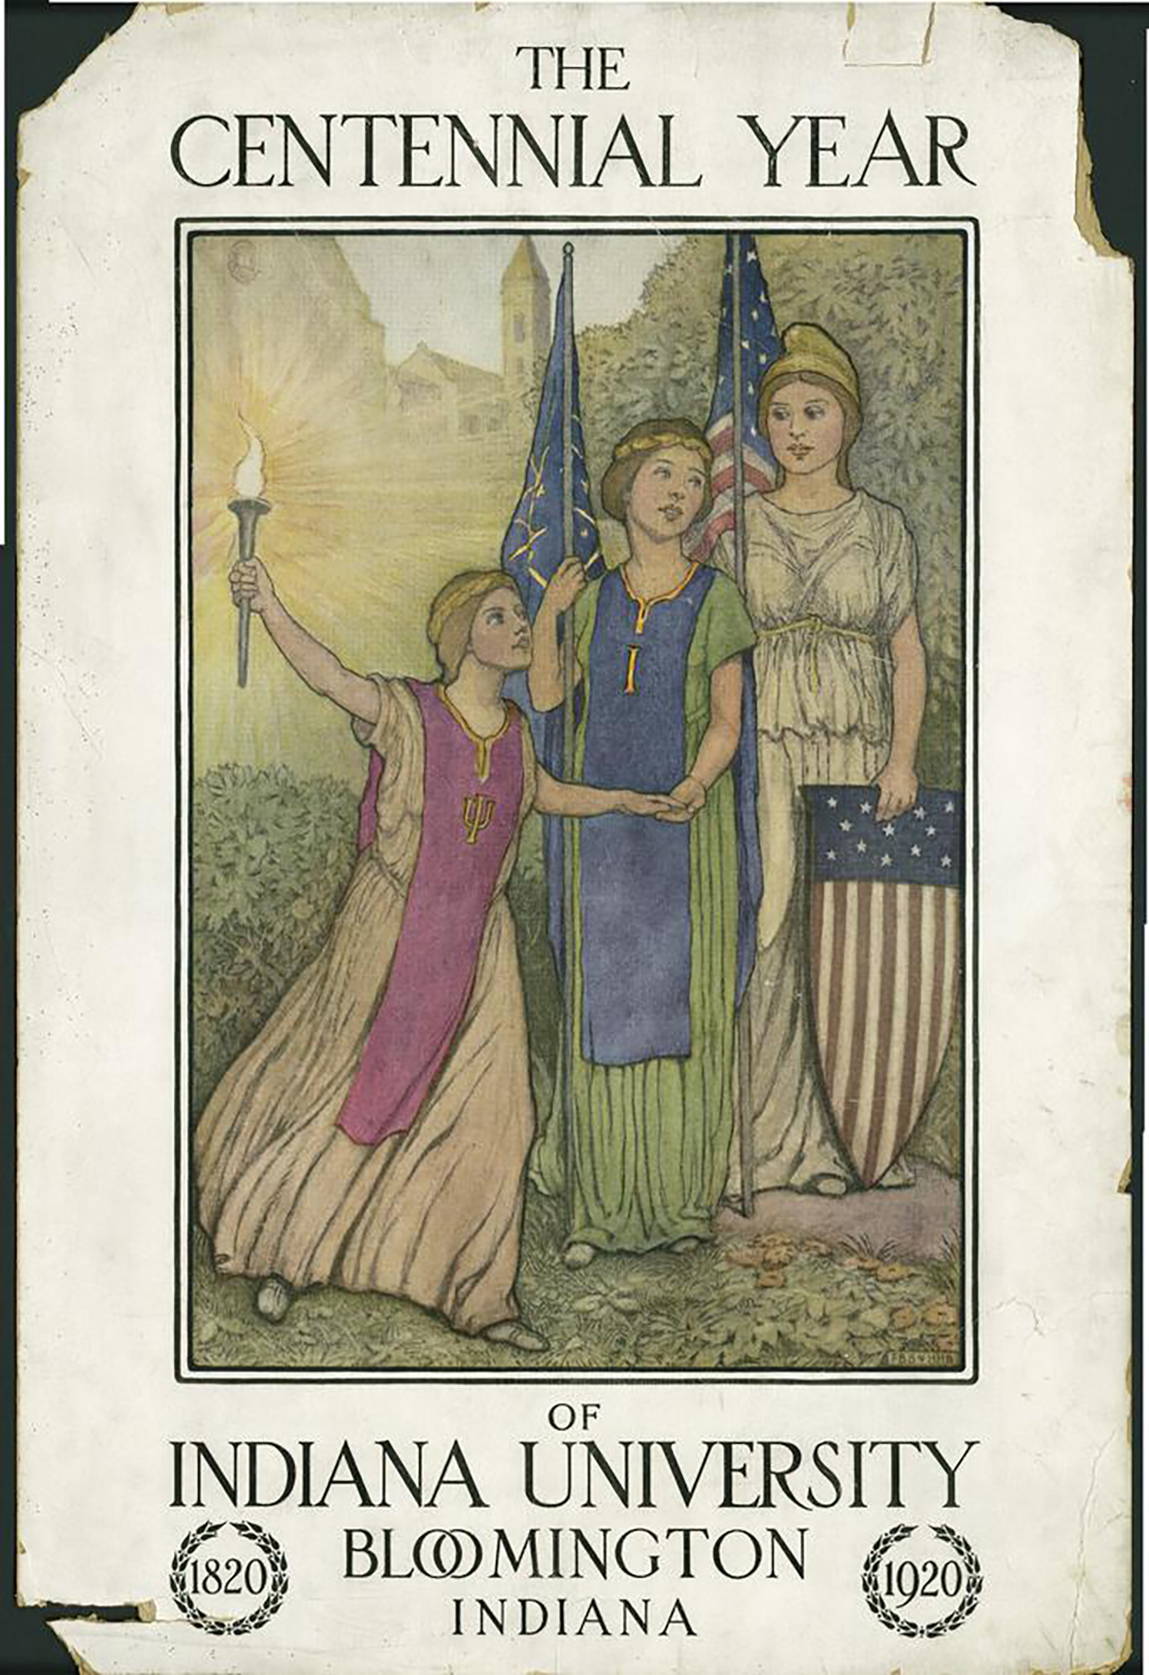
\includegraphics[width=0.6\linewidth,height=\textheight,keepaspectratio]{images/centennialrev.jpg}

}

\caption[Poster for the Centennial Pageant in 1920]{Poster for the
Centennial Pageant in 1920. With the campus bell tower in the
background, feminine spirits occupy the foreground, left to right,
symbolizing Indiana University, the State of Indiana, and the United
States of America. \textbf{© Indiana University. Image from the
\href{https://libraries.indiana.edu/university-archives}{IU Archives}.}}

\end{figure}%

\bookmarksetup{startatroot}

\chapter{The Keeper of University History}\label{sec-eight}

\begin{figure}[H]

{\centering 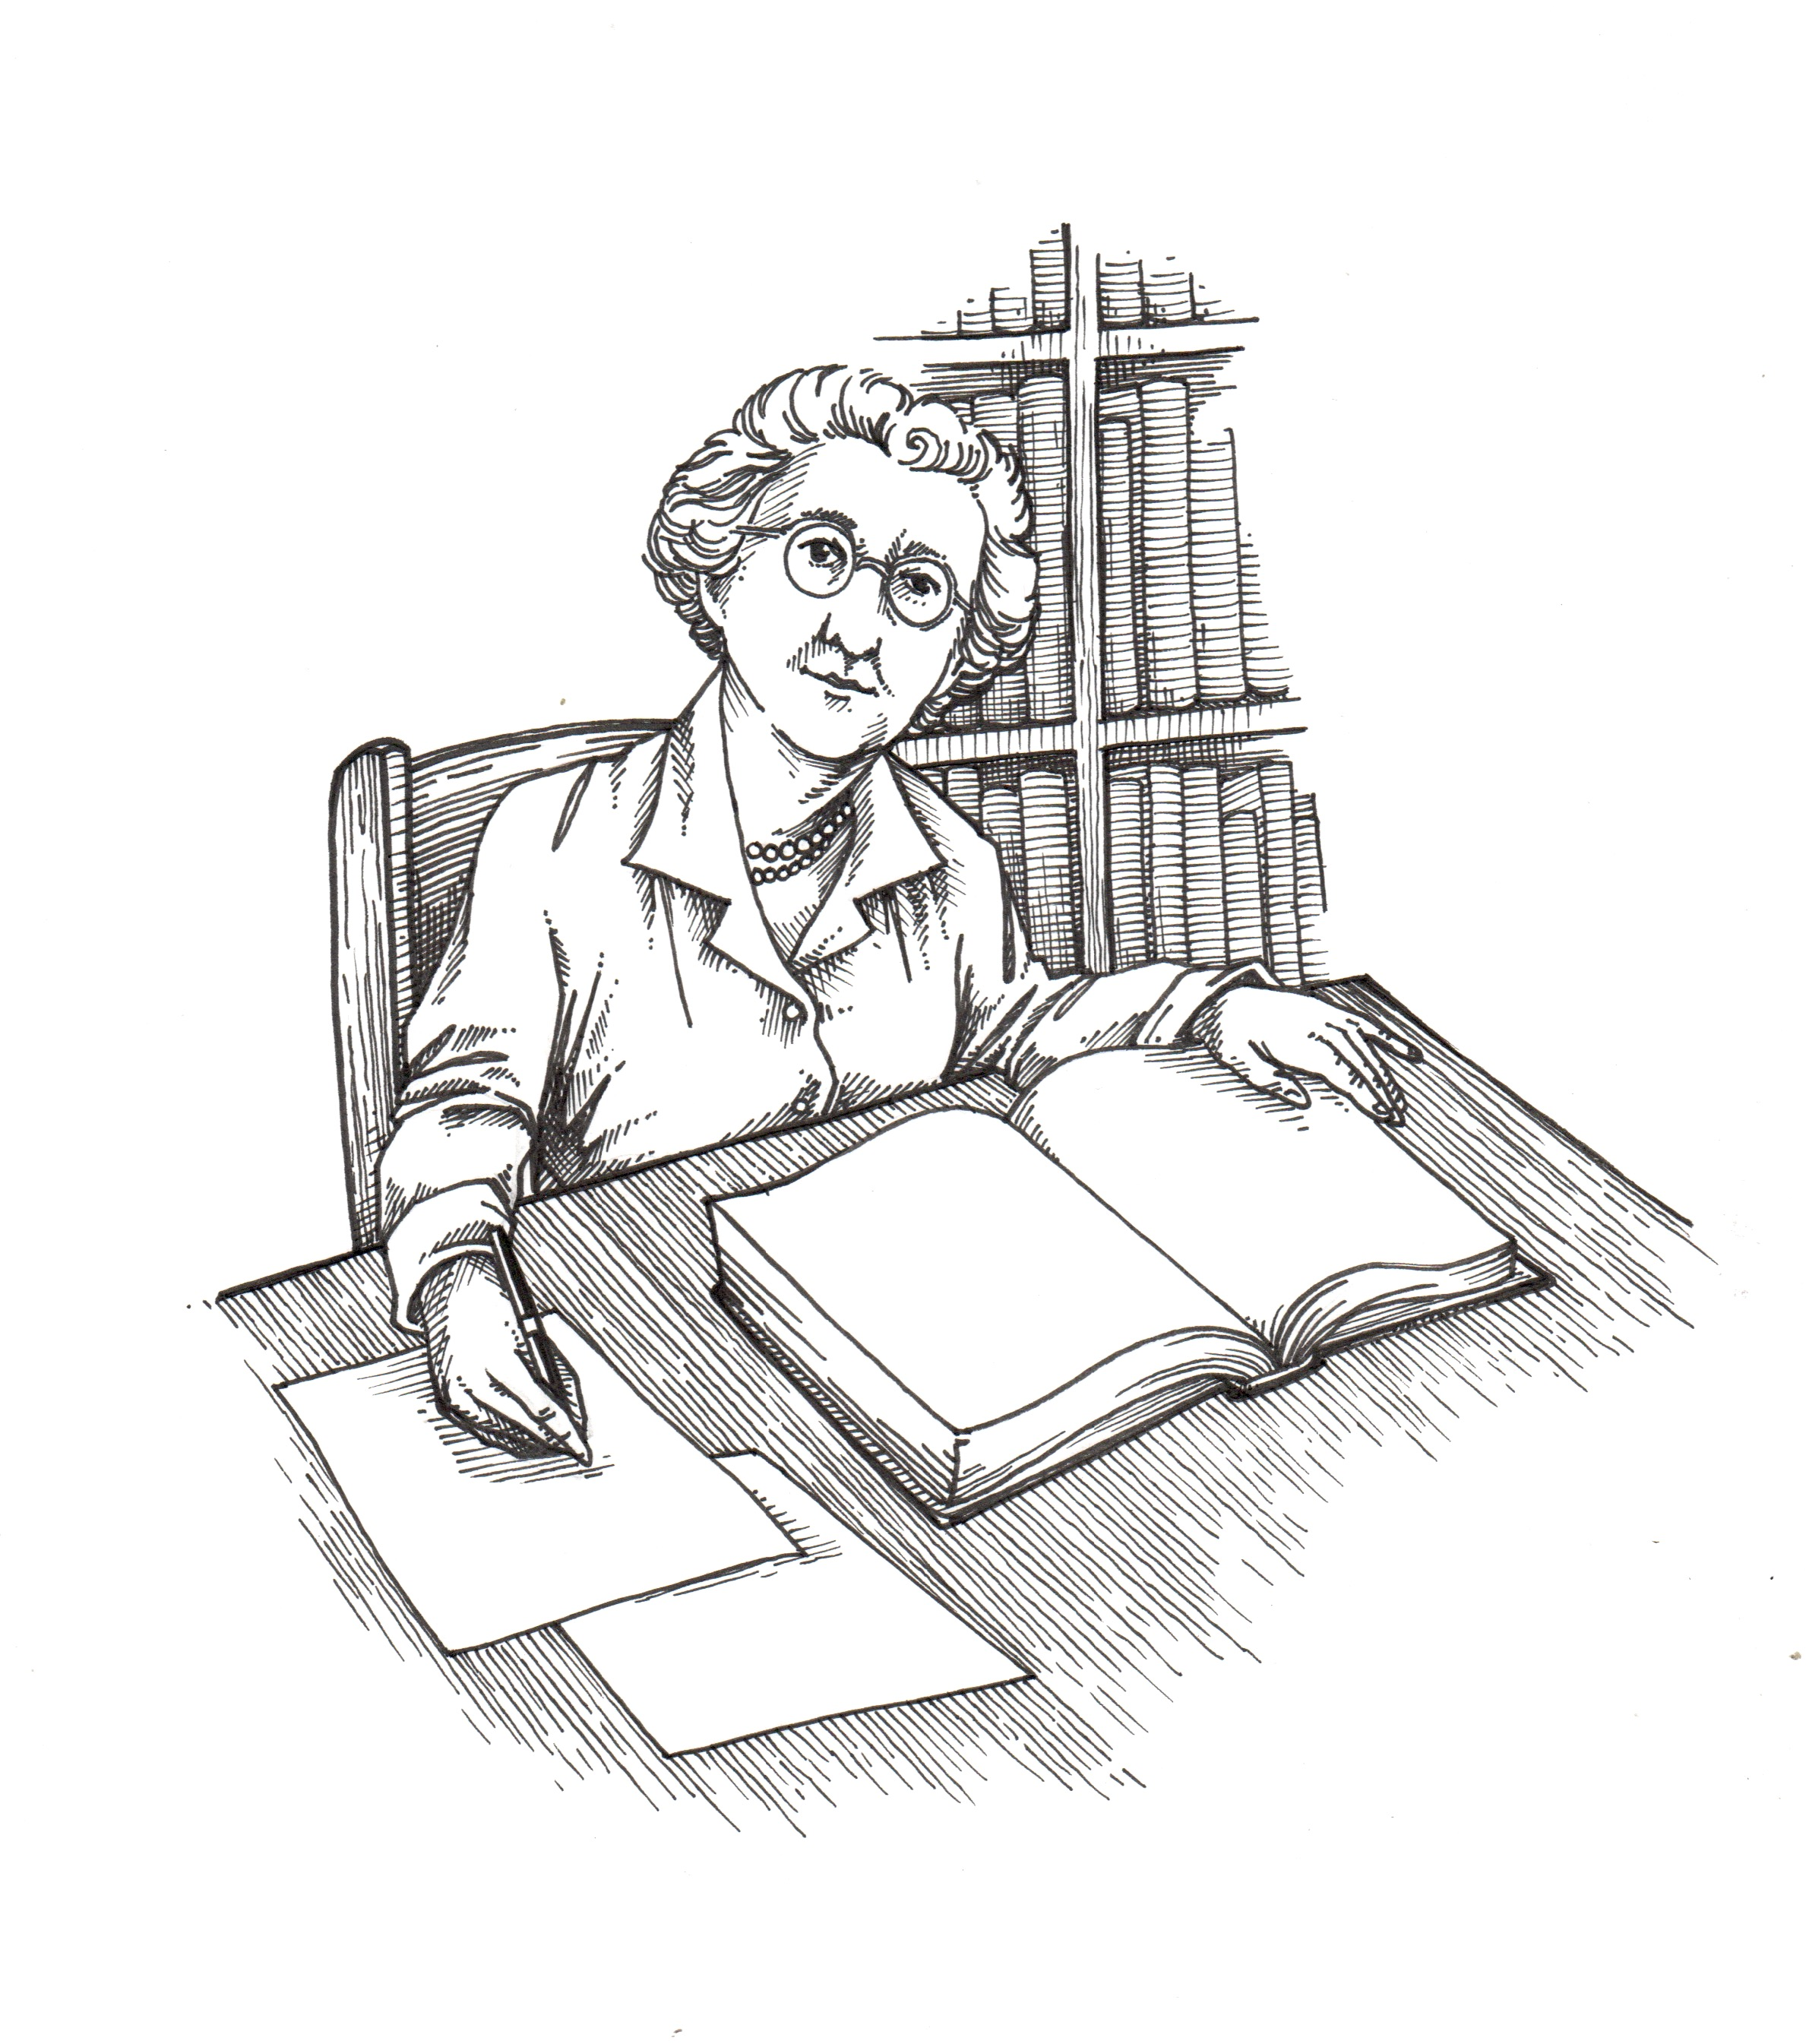
\includegraphics[width=0.6\linewidth,height=\textheight,keepaspectratio]{images/miu8.jpeg}

}

\caption{Ivy L. Chamness}

\end{figure}%

\epigraph{
If the history of Indiana University is ever written, much of it must needs be culled from the catalogues, papers, commencement and other programs which have been preserved by individuals as well as by the University. The mind of man runneth not back to the earliest days, and some of the University records were destroyed in the fires of 1854 and 1883. Extant records, moreover, give us only official acts, and it is to periodicals of the times and to programs of "activities" that we must turn for a picture of college life in those far-off days, seemingly so very, very unlike the present.  }
{---Ivy L. Chamness, "Indiana University in Earlier Days: I. As Reflected in Commencement and Exhibition Programs"}

The first person to hold the position of editor of publications at
Indiana University, Ivy Leone Chamness (1881--1975), is little
remembered today. Her career began before the First World War and
concluded after the Second, from 1914 to 1952. She made signal
contributions to the writing, editing, and production of nearly all IU
official communications, chief among them the periodic catalogs,
bulletins, and registers. In addition, Chamness became the sole editor
of the \emph{Indiana University Alumni Quarterly} soon after it was
begun in 1914. She made a special effort to nurture the understanding of
the institution by making the \emph{Alumni Quarterly} the journal of
record for IU's history. She worked closely with the two preeminent
architects of the modern university, William Lowe Bryan (president
1902--37) and Herman B Wells (president 1937--62), to shape its textual
image to students, faculty, and staff as well as to attract and foster
loyalty among its alumni and friends. When she was called on to assist
elderly faculty historians as a developmental editor for long-delayed
projects, she did not hesitate to lend her talents and skills. Yet she
is barely remembered, remaining in the background as a hidden figure
whose editorial and communicative work for the university did much to
advance its fortunes during the first half of the twentieth century. In
her role as the keeper of campus history, Chamness's efforts to edit,
publish, and make known the history and culture of Indiana University
are well worth noting.

\section{From Student to Employee}\label{from-student-to-employee}

Chamness was born on December 3, 1881, in Hagerstown, Indiana, near
Richmond, the county seat of Wayne County. She graduated from Hagerstown
High School in 1900 after suffering a bout of malaria two years before.
She and her sister, Gracie May, enrolled at IU in 1902, during the first
year of the administration of President William Lowe Bryan, and joined a
student body of 750. Ivy graduated in 1906, majoring in English, and
read the class poem at Senior Day. In the summer she wrote to the IU
registrar, John W. Cravens, for help finding a job teaching English.
With no teaching experience, in the fall of 1906, she landed a position
at the Carlisle School in Sullivan County near Terre Haute. She
contracted a serious case of diphtheria in the winter. During the next
few years, Chamness was employed as an English teacher at a couple of
schools in her home county, and in 1911, she got a job in Indianapolis
at the Bobbs-Merrill Publishing Company, working in the law books
division as a junior editor. The next year, she was on a streetcar that
wrecked and injured twenty-one people, but she escaped with only bruised
arms. After three years at Bobbs-Merrill, she was hired by IU as
assistant editor of publications. She was not quite thirty-three years
old, becoming ``the first full-time appointee in this work.''\footnote{\citeproc{ref-myers1952a}{Myers,
  \emph{History of Indiana University}, 1952, 170}.}

When Chamness started work at IU in 1914, there was no title of ``editor
of publications''; the responsibilities had been folded into the duties
of John Cravens, university registrar and secretary to the board of
trustees, since the turn of the century.\footnote{Cravens served as
  registrar from 1895 to 1936, secretary to the board of trustees from
  1898 to 1936, and secretary to the university from 1915 to 1936.} He
was a trusted member of the small administrative staff and known to
nearly all in the university community. In fact, Chamness had written to
him several times for job advice after graduation. Cravens was appointed
to the additional post of secretary to the university in 1915, soon
after Chamness's arrival on staff.

\section{\texorpdfstring{Early Years at the \emph{Alumni
Quarterly}}{Early Years at the Alumni Quarterly}}\label{early-years-at-the-alumni-quarterly}

Chamness witnessed the infancy of the \emph{Indiana University Alumni
Quarterly}, born in 1914. The Alumni Association of Graduates and Former
Students of Indiana University, as it was known formally, had tried
various ways to communicate with the alumni in the past, and the
quarterly was designed to be an expanded channel, with articles of
current interest, news of the university, book reviews and literary
notes, and class notes arranged by graduation year. The reform of the
association also included a full-time executive secretary to oversee
strategic plans as well as day-to-day operations.

The \emph{Alumni Quarterly}'s initial editor was Samuel Bannister
Harding, a history professor. A prolific author, he had edited the
historical sketch \emph{Indiana University, 1820--1904} ten years
before.\footnote{\citeproc{ref-harding1904a}{\emph{Indiana University,
  1820--1904}}.} The first issue started with an examination of the
institutional beginnings of IU, with an article on ``The Seminary
Period'' by the late David D. Banta. With the printing of all of Banta's
Foundation Day addresses for the first time---six in all---in the first
six issues of the \emph{Alumni Quarterly}, his historical viewpoint was
given fresh life to a new generation, and its publication in an organ of
the university gave it an official imprimatur.

In the fourth issue, published in October 1914, Chamness contributed a
book review of \emph{Readings in Indiana History}, edited by a committee
of the Indiana State Teachers Association and published by IU's new
Extension Division. By that time, she was working at IU as assistant
editor of publications (her book review was submitted months earlier).

In 1915, Chamness jumped in to help the fledging \emph{Alumni Quarterly}
with volume 2 and began to edit the section ``Alumni Notes by Classes.''
The head note for that section contained a recurring plea: ``It is
urgently requested that each class proceed forthwith to the choice of a
permanent class secretary who will undertake news of his class, and
transmit it to the Editor.'' Taking her own advice, Chamness began
serving as the class of 1906 secretary.\footnote{\citeproc{ref-chamness1915b}{{``Alumni
  Notes by Classes,''} ed. Ivy Leone Chamness, \emph{Indiana University
  Alumni Quarterly} 2, no. 2 (April 1915): 207}.}

For the July 1915 issue, history professor James A. Woodburn continued
the historical narrative begun by Banta. He published a total of eight
articles over the next two years, dealing with the university's
development during the period 1840 to 1860. Thus, by the end of the
\emph{Alumni Quarterly}'s first four years, a total of fourteen
historical articles were published, starting a lasting trend.\footnote{\citeproc{ref-woodburn1940a}{\emph{History
  of Indiana University}, 1940, v}.}

Beginning with volume 3 in 1916, Chamness appeared on the masthead as
assistant editor, alongside the alumni secretary, R. V. Sollitt, as
managing editor, and Professor Samuel B. Harding as advisory editor.
Chamness was lauded by Sollitt for her ``fine cooperation\ldots in
getting out the Quarterly,'' with ``vigilance and zeal in securing news
items of the alumni,'' which had made her department one of the most
important.\footnote{\citeproc{ref-iuaq1916a}{{``Work of the Alumni
  Council,''} \emph{Indiana University Alumni Quarterly} 3, no. 3 (July
  1916): 401}.} In addition to her part-time work on the \emph{Alumni
Quarterly}, Chamness had been given more responsibility in her main job
of editing official IU publications. Because of her proficiency, in
1917, she was made editor of publications for the university. But the
recognition of her increasing competency was marred by the behavior of
her administrative superiors at the alumni association.

In July 1918, Sollitt took a leave of absence in New York City, and
Chamness took on his duties. He was still listed as managing editor, and
she assumed that they would communicate regularly while he was away, but
he failed to write a single letter. So, she was responsible for the
entire operation: ``procuring and editing of all signed articles, the
writing of all unsigned articles, and the proofreading.''\footnote{\citeproc{ref-chamness1920a}{{``Letter
  to William Lowe Bryan''} (Indiana University Archives, May 11, 1920).
  IUA/C286/B54}.} After putting up with the silent treatment for nine
months, she wrote to the alumni council about the situation, requesting
``a change in the statement of editorship'' to insert her name as
``editor-in-chief'' while Sollitt was away.\footnote{\citeproc{ref-chamness1919a}{{``Letter
  to Alumni Council''} (Indiana University Archives, March 22, 1919).
  IUA/C286/B54}.} Adding insult to injury, two months later and yet to
receive a reply to her request, a different acting editor was named. She
complained to President Bryan about her ``arduous and gratuitous
service'' on the quarterly being ``repudiated in a sense, that is by the
appointment over my head of someone without any experience in the
work.''\footnote{\citeproc{ref-chamness1919b}{{``Letter to William Lowe
  Bryan''} (Indiana University Archives, June 18, 1919). IUA/C286/B54}.}
Her complaint did bring some extra compensation but no acknowledgment of
the legitimacy of her criticism.

Sollitt's leave turned into a separation, and in 1919, the alumni
council selected a new secretary---Humphrey Mahan Barbour---who became
the \emph{Quarterly}'s managing editor, and Chamness was promoted to
associate editor. The council also directed Barbour to send Chamness ``a
letter of deep appreciation for her great and generous services in
acting as the sole editor of the \emph{Quarterly} in the absence of
Mr.~Sollitt.''\footnote{\citeproc{ref-iuaq1919a}{{``Alumni Council
  Meetings,''} \emph{Indiana University Alumni Quarterly} 6, no. 3 (July
  1919): 394}.} That was a measure of affirmation of her grievance.

When Sarah Parke Morrison, the first female student and graduate of
Indiana University, died in Indianapolis in July 1919, Chamness
republished Morrison's reminiscences from the \emph{Indianapolis Star}
in the \emph{Alumni Quarterly}. Under the title ``Some Sidelights of
Fifty Years Ago,'' Morrison recounted the reasoning that brought her to
the university in 1867, noting the fact that her brother Robert entered
twenty years before, ``though I was two years his senior.'' Her father,
an IU trustee, supported her education, first at home and then at Mount
Holyoke, a female seminary at the time, and Vassar College, and finally
at IU, graduating in 1869. ``But my school days were about over,''
Morrison wrote. ``I could only rejoice at the opening prospect for young
women as already exemplified,'' concluding with a dose of sarcasm, ``and
sit at home.''\footnote{\citeproc{ref-morrison1919a}{{``Some Sidelights
  of Fifty Years Ago,''} \emph{Indiana University Alumni Quarterly} 6,
  no. 3 (July 1919): 530}.}

\section{IU Centennial}\label{iu-centennial}

Indiana University celebrated its centennial birthday on January 20,
1920. IU counted around 7,000 alumni, along with 17,000 former students.
Yet, despite a recent membership drive, the alumni association possessed
about 2,000 members.

Chamness became even busier with editing and publishing items
surrounding the commemoration. When alumni secretary Barbour left in
June 1920, she was appointed acting editor of the \emph{Alumni
Quarterly}. The following year, the alumni council belatedly
acknowledged her value and steady presence within the parade of
short-term managing editors---all men, not coincidentally---and promoted
her to the position of editor. Simple, unadorned ``editor''---of which
she had been doing the work for half a decade already. ``Miss Chamness
has been actively engaged with the editorial work of the
\emph{Quarterly} for a number of years and it is fitting and proper that
she should be given the position as editor of the \emph{Quarterly}
because of her long and efficient services in connection with
it.''\footnote{The decision was made June 6 to take effect on September
  1. \citeproc{ref-iuaq1921a}{{``Ivy Chamness to Edit Quarterly,''}
  \emph{Indiana University Alumni Quarterly} 8 (1921): 331--32}.}
Moreover, the new alumni secretary said, ``Too much cannot be said of
the services of Miss Chamness in connection with the \emph{Alumni
Quarterly}. For years she has worked on the \emph{Quarterly} under the
title of Associate Editor when in fact, for all information I can
ascertain, she has practically edited the magazine. The Alumni Council
owes Miss Chamness a vote of thanks for her efficient
services.''\footnote{\citeproc{ref-iuaq1921a}{{``Ivy Chamness to Edit
  Quarterly,''} 332}.} Her delayed appreciation fit a common historical
pattern of under-recognition and segregated employment endured by women.

Chamness reported on the voluminous activities of the Centennial
Commencement in the July 1920 issue of the \emph{Alumni Quarterly}. The
festivities lasted for nearly a week, from the baccalaureate address on
May 30 to the ninety-first annual commencement on June 4. ``The week was
crowded full of interesting events'' in which a record number of alumni
attended. ``The campus was lovely, as always, and the weather on most
days favorable,'' and ``everyone was happy to be here,'' she
wrote.\footnote{\citeproc{ref-iuaq1920a}{{``The Centennial
  Commencement,''} \emph{Indiana University Alumni Quarterly} 7 (1920):
  370}.}

The production of \emph{Indiana University, 1820--1920: Centennial
Memorial Volume} fell into the capable hands of Chamness (then editor of
university publications). Part one reprinted the six articles by Banta
on the history of the university from the \emph{Alumni Quarterly}. Part
two comprised thirteen addresses presented at the Centennial Educational
Conference in early May, on topics ranging from science to spirituality,
all relating to education. The final part reprinted Chamness's report on
the Centennial Commencement, originally published in the \emph{Alumni
Quarterly}.\footnote{\citeproc{ref-chamness1921a}{\emph{Indiana
  University, 1820--1920}}.} Widely distributed, the book became a
lasting memento of the occasion. It revealed the ceremonial use of IU
history as a background to current views and contentions of possible
futures connected to university life, addressed by a parade of
establishment figures. Only in the last section did the commentary turn
to more quotidian activities on the local scene.

As the university continued to grow under the Bryan administration,
Chamness kept pace with the demands of her position as chief editor of
the bulletins, catalogs, and other university publications.

\section{``Mother of College
Presidents''}\label{mother-of-college-presidents}

Less than a year after the IU centennial celebration, Chamness wrote a
short article titled ``Indiana University---Mother of College
Presidents'' for the journal \emph{Educational Issues}. ``Her
graduates,'' she wrote, ``have been called to the presidencies of
universities, colleges and normal schools from Maine to California, from
Minnesota to Florida.''\footnote{\citeproc{ref-chamness1921b}{{``Indiana
  University---Mother of College Presidents,''} \emph{Educational
  Issues} 2, no. 8 (1921): 28--29}.} There might be larger universities
who have produced more, but, she added, ``considering the size and age
of the institution, the University has an unusually large proportion of
men at the head of institutions of higher learning.'' The article
included a list of twenty-five college and university presidencies held
by IU alumni, including state and private universities, normal schools,
and denominational colleges.

To explain this trend, Chamness cited a policy credited to David Starr
Jordan, IU president from 1885 to 1891. He encouraged promising
undergraduate alumni to obtain graduate training, either in the east or
Europe, before returning to Bloomington to qualify as members of the
faculty. When Jordan left to become the inaugural president of Stanford,
he took six faculty members with him, some future presidents among them.
Concluding on a bittersweet note, Chamness wrote, ``Since that time
increasing numbers of faculty members and alumni have left the
University and the state to become educational leaders in other fields.
Their fellow alumni rejoice in their progress and advancement in the
educational world, but feel regret\,that the University and the state of
Indiana must be deprived of their leadership.''\footnote{\citeproc{ref-chamness1921b}{28--29}.}

The next year, Chamness republished her article in the \emph{Alumni
Quarterly}, adding a few more names to the list of
presidents.\footnote{\citeproc{ref-chamness1922a}{{``Indiana
  University---Mother of College Presidents,''} \emph{Indiana University
  Alumni Quarterly} 9 (1922): 46--49}.} Over time, she would continue to
add names, and her assessment that the institution was the ``mother of
college presidents'' became embedded in IU's historical
identity.\footnote{For example, (\citeproc{ref-chamness1923a}{{``More
  College Presidents,''} \emph{IU Alumni Quarterly} 10 (1923): 334});
  (\citeproc{ref-chamness1923b}{{``Another College President,''}
  \emph{IU Alumni Quarterly} 10 (1923): 512});
  (\citeproc{ref-chamness1938a}{{``Another College President,''}
  \emph{IU Alumni Quarterly} 25 (1938): 59}). See also Capshew,
  \citeproc{ref-capshew2011a}{{``Indiana University as the {`Mother of
  College Presidents'}''}}.}

As a follow-up to the IU centennial, Registrar John Cravens noted the
1922 centennial of the university's first building---the Seminary
Building---and published a series of three articles in the \emph{Alumni
Quarterly} detailing the architectural history of Indiana University. He
was careful to document sources to the written record, but much
information depended on the oral tradition as well as his personal
experience reaching back to the 1890s.\footnote{\citeproc{ref-cravens1922a}{{``Buildings
  on the Old and New Campuses of Indiana University,''} 1922};
  \citeproc{ref-cravens1922b}{{``Buildings on the Old and New Campuses
  of Indiana University,''} 1922};
  \citeproc{ref-cravens1922c}{{``Buildings on the Old and New Campuses
  of Indiana University,''} 1922}.}

Five years later, in 1927, Cravens published the results of his study of
the IU trustees, which totaled 148 individuals, updating an earlier list
found in Wylie's 1890 historical catalog. He noted the silver
anniversary of the administration of President Bryan, who had served
longer than any other president. In addition to outlining the trustee
board's evolving structure, he listed some of the accomplishments and
official positions of individual trustees, including service in state
and national governments.\footnote{\citeproc{ref-cravens1927a}{{``The
  Trustees of Indiana University,''} \emph{Indiana University Alumni
  Quarterly} 14 (1927): 465--83}.} Both of Cravens's publications were
timely contributions to conversations about the past among the IU
community as well as valuable additions to the permanent historiography.

In 1928, Chamness completed a master's degree in journalism. Drawing on
her daily work, she conducted a thesis titled ``A Study of Editorial
Matters in the Catalogs of the Members of the National Association of
State Universities.''\footnote{\citeproc{ref-chamness1928a}{{``A Study
  of Editorial Matters in the Catalogs of the Members of the National
  Association of State Universities''} (Indiana University, 1928).
  Master's thesis, Indiana University}.} The existing literature was
scant---only three publications---and her approach was strictly
empirical.

Based on responses from forty-nine institutions and their catalogs, she
compared typography and form, information and its arrangement, and
miscellaneous matters. In the last section, Chamness discussed
editorship, suggesting, ``Editors are usually a modest lot; they almost
have to be. They become quite accustomed to doing hard work to which no
name or someone else's name is attached. Editors of college catalogs
seem to be no exception. Many of these publications give the reader no
hint as to who is responsible, and, indeed, if something goes wrong
'twixt manuscript and printing press, the editor may well be content
with his anonymity.''\footnote{\citeproc{ref-chamness1928a}{127.
  Master's thesis, Indiana University}.}

Her study revealed a wide array of answers to the question ``Who is
responsible for editing your catalog?'' ranging from administrative
staff to members of a committee. About 60 percent of the institutions
surveyed had an advisory committee. She noted that ``the best practice
would call for an advisory committee to discuss and determine matters of
policy, which the editor could carry out.''\footnote{\citeproc{ref-chamness1928a}{130.
  Master's thesis, Indiana University}.}

She completed her 150-page thesis with a one-paragraph conclusion
suggesting ways to improve the college catalog, focusing on the
important role of editor. If the work falls to a committee, ``uniformity
in details will be well nigh impossible. There are many, many minutiae
which must be watched, and patience, endurance, and eternal vigilance
are prerequisite to the work of editing a college catalog.''\footnote{\citeproc{ref-chamness1928a}{150.
  Master's thesis, Indiana University}.}

\section{``In Earlier Days''}\label{in-earlier-days}

In 1929, Chamness launched an article series under her byline in the
\emph{Alumni Quarterly} with the general title ``Indiana University in
Earlier Days.'' It surveyed the historical documents that Professor
Emeritus Woodburn had recently given to the university, consisting of
old catalogs and programs, and issues of the \emph{Indiana Student}.
Some of the material was collected by his father, James W. Woodburn, who
graduated in 1842 and served as a faculty member before his early death.
Other documents were from his own collection, dating back to his student
days in the 1870s, augmented by another collection from Professor Frank
Andrews. Revealing her penchant for writing and her understanding of the
importance of documentary sources, Chamness introduced the series by
saying official publications are important, but ``extant records,
moreover, give us only official acts, and it is to periodicals of the
times and to programs of `activities' that we must turn for a picture of
college life in those far-off days, seemingly so very, very unlike the
present.''\footnote{\citeproc{ref-chamness1929a}{{``Indiana University
  in Earlier Days: I. As Reflected in Commencement and Exhibition
  Programs,''} \emph{Indiana University Alumni Quarterly} 16, no. 1
  (1929): 33}.}

IU's institutional archives, such as student records and board of
trustees' minutes, were woefully incomplete due to campus fires in 1854
and 1883 that obliterated the bulk of them. Theophilus Wylie's
painstaking work for the 1890 historical catalog, \emph{Indiana
University, Its History from 1820, When Founded, to 1890}, partially
remedied the damage by compiling lists of students, faculty, and
trustees, but records of the early history of student life were gone.
Chamness attempted to reconstruct this lost history using the
collections of historical materials recently donated to the university.
What emerged were fascinating glimpses into nineteenth-century
collegiate life in Bloomington.

Chamness described the students of the 1840s to the 1890s by using past
commencement programs.\footnote{\citeproc{ref-chamness1929a}{{``Indiana
  University in Earlier Days,''} 1929}.} Each graduating student had to
deliver a public speech---a commencement oration---at the graduation
ceremonies. The subjects were varied. Chamness characterized early
graduates as being abstract, ambitious, broad, and inquisitive,
reminding readers that those students carried the same traits as
students of today. Student solidarity and the practice of protesting
perceived injustice remained similar, Chamness suggested, ``even in
those days, for we read that sixty-three fellow-students proposed to go
with a student who, it was claimed, was dismissed without
investigation.''\footnote{\citeproc{ref-chamness1929b}{{``Indiana
  University in Earlier Days: II. As Reflected in Early Issues of the
  \emph{Indiana Student},''} \emph{Indiana University Alumni Quarterly}
  16, no. 2 (1929): 218}.} Even past student newspapers, which looked
significantly different from the contemporary \emph{Indiana Daily
Student}, showcased the similarities between present and past collegiate
life.\footnote{\citeproc{ref-chamness1929b}{Chamness, 199}.} While the
\emph{Indiana Student} advertised ``activity tickets'' for music
concerts and the Union Series, one of the past newspapers, \emph{The
Student}, advertised opportunities to attend lectures, an occasion that
provided students with entertainment and the chance to hear renowned
speakers.\footnote{\citeproc{ref-chamness1931a}{Ivy Leone Chamness,
  {``Indiana University in Earlier Days: IV. As Reflected in Issues of
  the \emph{Indiana Student} in the Nineties,''} \emph{Indiana
  University Alumni Quarterly} 18, no. 2 (1931): 170}.} Even with the
passage of many years, continuities can be observed in collegiate life.

Despite such similarities, however, Chamness acknowledged that college
life had evolved over time and did not mirror the present exactly. The
old \emph{Indiana Student} newspaper had a literary cast, with
literature, reviews, and letters exchanged among the IU community. In
contrast, the contemporary \emph{Indiana Daily Student} emphasized news,
sports, and entertainment.\footnote{\citeproc{ref-chamness1929b}{Chamness,
  {``Indiana University in Earlier Days,''} 1929, 202}.} Chamness
reprinted the 1878 university rules for students. She noted that
present-day departments in the university did not have equivalents of
two of the original departments: civil engineering and mental, moral,
and political philosophy.\footnote{\citeproc{ref-chamness1934a}{Ivy
  Leone Chamness, {``Indiana University in Earlier Days: VII. As
  Reflected in Official Publications,''} \emph{Indiana University Alumni
  Quarterly} 21, no. 2 (1934): 42}.}

The seventh and last article in the ``Indiana University in Earlier
Days'' series appeared in 1934.\footnote{\citeproc{ref-chamness1929a}{Chamness,
  {``Indiana University in Earlier Days,''} 1929};
  \citeproc{ref-chamness1929b}{Chamness, {``Indiana University in
  Earlier Days,''} 1929}; \citeproc{ref-chamness1930a}{Ivy Leone
  Chamness, {``Indiana University in Earlier Days: III. As Reflected in
  the Issues of the \emph{Indiana Student} in the Nineties,''}
  \emph{Indiana University Alumni Quarterly} 17, no. 1 (1930): 22--38};
  \citeproc{ref-chamness1931a}{Chamness, {``Indiana University in
  Earlier Days,''} 1931}; \citeproc{ref-chamness1931b}{Ivy Leone
  Chamness, {``Indiana University in Earlier Days: V. As Reflected in
  Historical Material Recently Given to the Institution,''}
  \emph{Indiana University Alumni Quarterly} 18, no. 1 (1931): 16--29};
  \citeproc{ref-chamness1933a}{Ivy Leone Chamness, {``Indiana University
  in Earlier Days: VI. As Reflected in Official Publications,''}
  \emph{Indiana University Alumni Quarterly} 20, no. 2 (1933): 159--68};
  \citeproc{ref-chamness1934a}{Chamness, {``Indiana University in
  Earlier Days,''} 1934}.} Chamness produced one hundred pages of
material, including programs from commencements, literary societies, and
other events; official catalogs; and student newspaper publications from
the last quarter of the nineteenth century. Chamness divided the
information up into three categories---programs (one article),
\emph{Indiana Student} (three articles), official publications (two
articles)---plus one miscellaneous article. It truly was a grab bag, but
it did contain valuable archival information for future historians. It
generated interest among the alumni and, in some cases, stimulated
responses that were subsequently published, adding more texture and
context to the documents.\footnote{For instance, Goodwin,
  \citeproc{ref-goodwin1930a}{{``The \emph{Indiana Student} and Student
  Life in the Early Eighties''}}.} Her respect for the documentary
record extended to the past, as evidenced by her thorough discussion of
historical documents pertaining to the university's past that had
survived to the 1920s.

\section{\texorpdfstring{Woodburn and \emph{History of Indiana
University}}{Woodburn and History of Indiana University}}\label{woodburn-and-history-of-indiana-university}

By 1933, Chamness had become actively involved in Woodburn's history of
Indiana University project. President Bryan asked her to work with
Professors Henry H. Carter and Albert L. Kohlmeier to prepare an article
on the history of the curriculum post-1904 for the history volume. She
also volunteered to prepare an index to the section ``News of the
University'' published in the \emph{Alumni Quarterly} to aid Woodburn's
research.\footnote{\citeproc{ref-iuaC286B54a}{Indiana University
  Archives, {``Finding Aid, Collection 286, Box 54''} (Bloomington, IN:
  Indiana University, n.d.). IUA/C286/B54}.} Nearly twenty years before,
she had worked with Woodburn when he published several articles in the
\emph{Alumni Quarterly}. Now, he was in his late seventies, living in
retirement in Michigan.

The history project dated to June 1929. Five years after Woodburn
retired from the faculty and moved to his wife's hometown of Ann Arbor,
President Bryan wrote him a letter, beseeching him to write ``some
chapters in the History of Indiana University during the period that you
have known it.'' Bryan and Woodburn had known each other since childhood
in Bloomington, and both entered IU as students in the 1870s. ``Your
reminiscences of the faculty and of the whole situation will be very
valuable,'' Bryan wrote, adding, ``You could continue your chapters as
long as you feel disposed, but I hope that you will not stop until you
have wound up with the chapter on your later years at the University.''
The president appealed to Woodburn's personal and family links to IU
history: ``You are yourself the link which connects the earliest years
of the University by your knowledge of some of the men at that time with
the present. It seems to me so wholly desirable from every point of view
that you should do this, that I can not bear you not to do
it.''\footnote{\citeproc{ref-bryan1929a}{{``Letter to James {A.}
  Woodburn''} (Indiana University Archives, June 17, 1929). IUA/C83/B3/F
  Publications, Galleys, \& Transcripts}.}

Woodburn responded affirmatively to this urgent plea, but the historical
project was slow to gain traction, exacerbated by his difficulty in
returning to Bloomington for archival research. The correspondence
between Woodburn and Bryan quickened again in 1934, with another
exchange of letters. Bryan ruefully promised to send a chapter that
could not appear in the book, illustrating ``the point that much of the
most interesting history cannot be written until everybody is dead who
had anything to do with it or who cares anything about it.'' To aid the
project, Bryan wrote to the faculty, present and past, asking for
biographical details, and announced that Woodburn was editor-in-chief
for the history project. Noting that a meeting of the board of trustees
was coming up, he asked Woodburn to prepare an outline of the book
project for their information.\footnote{\citeproc{ref-bryan1934a}{{``Letter
  to James {A.} Woodburn''} (Indiana University Archives, November 17,
  1934). IUA/C83/B3/F Publications, Galleys, \& Transcripts}.}

In 1935, Woodburn obliged by sketching an outline, noting that ``the
History has been carried to about 1887,'' the end point of Wylie's 1890
historical catalog. The proposed work would have several authors, mostly
faculty and staff, writing about various schools, the athletic program,
student life, the library, buildings and grounds, and the trustees. The
sketch had sixteen items, with eighteen authors contributing.

In keeping with Woodburn's conception of history as a container of the
past, authoritatively authored, he suggested including Judge Banta's
historical articles as well as his own---seen as a continuation of a
singular historical record. Woodburn set himself the task of covering
the period from 1856 (the termination point of his earlier work) up to
the turn of the twentieth century and the start of the Bryan
administration soon afterward.

In addition to Banta and Woodburn, the outline included sections on:
trustees and the physical plant (John Cravens), curriculum (Henry Carter
and Albert Kohlmeier), medical school (Burton Myers), law school
(unspecified), music (Winfred Merrill and John Stempel), journalism and
the \emph{Indiana Student} (Joseph Piercy and Walter French), presidents
and faculty (Mrs.~John Cravens), university publications (Ivy Chamness),
athletics (Charles Sembower and John Sembower), school of education
(Lester Smith), fraternities (Karl Fischer), the library (William
Alexander and Estella Wolf), and reminiscences (William L. Bryan). As
Woodburn put more time in the project, he came to agree with President
Bryan about its priority, admitting in 1935: ``I have let this thing
drag on without doing much at it, but now I recognize, with you, that it
should be pushed forward to completion within the year, if
possible.''\footnote{\citeproc{ref-woodburn1935a}{{``Letter to William
  Lowe Bryan''} (Indiana University Archives, February 28, 1935).
  IUA/C83/B3/F Publications, Galleys, \& Transcripts}.}

Editor Chamness, still busy with endless rounds of editing of IU
catalogs and bulletins, wrote a note to a faculty wife about some alumni
association business in 1935: ``I began my work on the \emph{Quarterly}
twenty-one years ago next fall with Volume I, No.~4. Surely my long
service and my financial support, probably longer than that of any on
the Council, deserve some consideration when a matter of this kind comes
up. One year I did all the work and ran another name as editor, said
editor never contributing one word.''\footnote{\citeproc{ref-chamness1935a}{{``Letter
  to Mrs. C. J. Sembower''} (Indiana University Archives, June 3, 1935).
  IUA/C84/B1/F Edited Manuscripts-Alumni Quarterly}.} She had moved on
from the injustice, but she never forgot.

Woodburn did not meet his self-imposed deadline, but in June 1936, he
convened a meeting of project authors in the Woodburn Room of the
Indiana Memorial Union building. The goal was to have completed
manuscripts on September 1, 1936. All of the authors reported that their
work was completed or in hand to meet the deadline except for one.
Fernandus Payne, dean of the graduate school, suggested that Woodburn,
as editor, should be authorized to cut or change any of the reports,
which received support.\footnote{\citeproc{ref-meetingWoodburn1936a}{{``Meeting
  in Woodburn Room, June 4, 1936,''} June 4, 1936. Folder: Publications,
  Galleys \& Transcripts, IUA/C83/B3/F, Indiana University Archives}.}
Despite the hopeful rhetoric, Woodburn's project continued to flounder.

\section{\texorpdfstring{From \emph{Alumni Quarterly} to \emph{Indiana
Alumni
Magazine}}{From Alumni Quarterly to Indiana Alumni Magazine}}\label{from-alumni-quarterly-to-indiana-alumni-magazine}

Having resided at 807 E. Tenth Street since 1933, Chamness lived with
her widowed mother. In January 1937, her mother died at age
seventy-nine, making Chamness the sole survivor of her immediate
family.\footnote{\citeproc{ref-iuaq1937b}{{``Alumni Notes by Classes:
  1906,''} \emph{Indiana University Alumni Quarterly} 24, no. 1 (1937):
  74}: ``Mrs.~Marvin E. Chamness, mother of Ivy L. Chamness, died at her
  home in Bloomington January 11 following an hour's illness.''} Other
changes were in store. On March 15, President Bryan, now seventy-six
years old and in office for thirty-five years, announced his retirement.
Taking the IU trustees by surprise, it set off an extended transition
period. In June, the trustees appointed dean of the business school
Herman Wells as acting president. The dean was young---he had just
turned thirty-five---but his character combined shrewd financial
judgment with deep empathy for everyone. The presidential search ended
nine months later, when the trustees elevated Wells to become the
eleventh president of Indiana University on March 22, 1938.\footnote{See
  Capshew, \citeproc{ref-capshew2012a}{\emph{Herman {B} Wells}}, Chapter
  5.}

In May, a new alumni magazine was proposed, touted as a way to get more
members. The alumni council sent a query card to 17,200 alumni, but only
759 cards were returned. Over 600 approved of the idea, while 71
disapproved. The recently appointed director of the IU News Bureau, E.
Ross Bartley, stated that ``the proposed monthly sounded like a very
excellent idea, that as good as the \emph{Quarterly} has been, it does
not quite fit in with the new spirit that Indiana has or compare to
other schools.'' Chamness, not reacting to the casual slight, stated
simply that she ``could do the book reviews, class notes, copy editing,
and proofreading.''\footnote{\citeproc{ref-iuaq1938a}{{``Commencement,
  1938,''} \emph{Indiana University Alumni Quarterly} 25, no. 3 (1938):
  298--337}, p.~309. Chamness's classmate ``Mrs.~Mary Hamilton Beck,
  '06, of Evanston, Ill. moved that a vote of appreciation be given to
  Miss Chamness for having given us a fine publication in the
  \emph{Quarterly}. Walter Crim seconded the motion and it was passed,''
  p.~316.}

So, after one hundred issues and a quarter century, the \emph{Indiana
University Alumni Quarterly} ceased publication with its October 1938
issue. Chamness had been identified with the publication since almost
the very beginning, keeping the communication channels between the
university and its alumni flourishing. For twenty-five years, it served
as the journal of record for university history, filling the
thirty-six-year gap between IU history books from 1904 to
1940.\footnote{Harding, \citeproc{ref-harding1904a}{\emph{Indiana
  University, 1820--1904}} and Woodburn,
  \citeproc{ref-woodburn1940a}{\emph{History of Indiana University},
  1940}.}

\section{\texorpdfstring{Publication of the \emph{History of Indiana
University}}{Publication of the History of Indiana University}}\label{publication-of-the-history-of-indiana-university}

Meanwhile, Chamness stepped up her work on Woodburn's history project,
as the new Wells administration made it among their priorities. She
requested more help in 1938 because of the increased workload. During
one of Woodburn's periodic visits, Chamness stated to Wells, ``I have
spent most of my time for two weeks in going over in a rather tentative
way the copy which Dr.~Woodburn prepared for his history.''\footnote{\citeproc{ref-chamness1938b}{{``Letter
  to Herman {B} Wells''} (Indiana University Archives, 1938).
  IUA/C213/B118}.}

In the interest of not delaying the volume further, it was decided to
save the draft sections authored by others and to concentrate on
finishing Woodburn's narrative. As the book took its final shape, it
became a hybrid. The first six chapters were authored by David Banta,
recycled from the early issues of the \emph{Alumni Quarterly}. The next
eight chapters were by Woodburn, again republished from the early
quarterly. The final eight chapters were new material by Woodburn,
covering the period from 1850 to 1902, the start of the Bryan
administration. Those chapters were a blend of historical analysis and
personal observation; Woodburn's memory encompassed the last quarter of
the nineteenth century. He also used primary sources and personal
correspondence to round out the narrative, sometimes quoting letters at
length. It was a brave performance, given Woodburn's age and declining
ability.

For her part, Chamness relished the intellectual and compositional
challenge. In a note to Woodburn, she declared, ``The work on this book
I regard as the most interesting task I have had or hope to have,'' and
added, ``I have put forth my supreme effort.''\footnote{\citeproc{ref-chamness1940a}{{``Letter
  to James {A.} Woodburn''} (Indiana University Archives, November 30,
  1940). IUA/C83/B4/F Testimonial Banquet/Correspondence}.} Although
Chamness was not acknowledged as the book's editor on the title page,
her extensive rewriting and editorial work was evident, and Woodburn
expressed heartfelt gratitude in the preface.\footnote{Woodburn,
  \citeproc{ref-woodburn1940a}{\emph{History of Indiana University},
  1940}, p.~v. A dozen years later, Chamness received retrospective
  acknowledgment as the editor of Woodburn's \emph{History of Indiana
  University}, in the succeeding volume. Myers,
  \citeproc{ref-myers1952a}{\emph{History of Indiana University}, 1952},
  p.~xiv.}

In 1940, the book was unveiled during a gala occasion---the Woodburn
Testimonial Dinner---held in Alumni Hall on November 30, Woodburn's
eighty-fourth birthday. President Wells, who had lived at the Woodburn
House for eight years and had warm relations with the emeritus
professor, wanted to thank Woodburn publicly for his lifetime of service
to the institution, culminating in the publication of the \emph{History
of Indiana University}, his last book.\footnote{Less than year
  afterward, in September 1941, Woodburn gave the Woodburn House to IU.
  Indiana University Board of Trustees,
  \citeproc{ref-botm1941a}{{``Minutes of the Board of Trustees of
  Indiana University, 25 September 1941--27 September 1941''}
  (Bloomington: Indiana University Archives \& Indiana University
  Libraries Digital Collections Services, September 27, 1941),
  \url{https://purl.dlib.indiana.edu/iudl/archives/iubot/1941-09-25}}.}
Over 300 people attended, and former students and colleagues wrote
letters of appreciation for the public presentation.

In his address at the Woodburn Testimonial Dinner, Woodburn recalled his
efforts to have David Banta's speeches on the early history of IU
published in the first issues of the \emph{Alumni Quarterly} and
modestly took credit for their preservation in print. As ``the real
historian of the University in its beginnings,'' stated Woodburn,
``Judge Banta had an historical sense and an historical scent. He knew
evidence. He went to the sources, and he wrote in such a style as to
make the facts as interesting as fiction.'' If Banta's work was the
starting point, ``at the other end of the enterprise came Miss Chamness,
who refuses to speak for herself, a most valuable editor, a fair and
generous critic.'' Woodburn only hinted at her enormous contributions to
the book: ``She has verified my statements or eliminated them. She has
worked with pencil and eraser and has done some of the best work with
the eraser. I wish again to acknowledge my obligations to her, which I
have done quite imperfectly in the preface.''\footnote{\citeproc{ref-woodburnTestimonial}{James
  A. Woodburn, {``Presentation of the \emph{History of Indiana
  University}, Volume {I} at the Woodburn Testimonial Dinner''} (Indiana
  University Archives, n.d.). IUA/C83/B4/F Woodburn, James}.} Chamness,
who had worked with Woodburn for nearly a quarter century, was gratified
by the public praise of her editorial skills. She would soon be involved
in the second volume of \emph{History of Indiana University}, assisting
another retired faculty member with the challenge of writing about
President Bryan's administration.

\section{\texorpdfstring{Myers and \emph{History of Indiana
University}}{Myers and History of Indiana University}}\label{myers-and-history-of-indiana-university}

No sooner was the Woodburn manuscript put to bed than Chamness turned
her attention to another book project: the history of the Bryan
administration. Supervised by retired professor of anatomy and medical
school dean Burton Myers, the second volume of \emph{History of Indiana
University} would cover the long administration of President Bryan from
1902 to 1937. A trusted member of President Bryan's inner circle, Myers
retired in July 1940, at age seventy, and he confidently took up the
mantle of amateur historian. Bryan and Myers had helped shape the early
IU School of Medicine and maintained a respectful friendship for
decades.

Myers had been working on a manuscript dealing with the history of
medical education off and on for several years before retirement. Within
the year following retirement, he was working on the history of the
Bryan administration. In April 1941, Myers and Wells had an exchange
about the project. Wells asked, ``For pay or labor for love?'' Myers
replied, stating his book project on medical education was a labor of
love, but the history project would be different:

\begin{quote}
For this other job I think a pay basis would be fair, tho' the ``labor
of love'' element would not be entirely lacking. It has not been lacking
during my years of connection with Indiana University. I have been happy
to try to give service worth twice as much as I was paid, which makes it
a sort of 50-50 proposition.\ldots What the pay basis should be---I will
be quite willing to leave to your judgement, and you may reserve
judgment, as long as you wish to assure yourself the effort is not a
flop.\footnote{\citeproc{ref-myers1941a}{{``Letter to Herman {B}
  Wells''} (Indiana University Archives, April 1, 1941). IUA/C213/B404/F
  Myers, Dean B. D.}}
\end{quote}

In the same exchange, Myers revealed a patronizing ambivalence about his
coworker: ``Miss Chamness as Associate Editor is all right. I have been
irritated by her at times, but we have gotten along reasonably well. I
realize that she has an experience and judgment that can be very
helpful.''\footnote{\citeproc{ref-myers1941a}{IUA/C213/B404/F Myers,
  Dean B. D.}}

Wells took this information in and added it to his elephantine memory.
For her part, Chamness approached the collaboration as a professional
task. Myers, a longtime administrator used to deference from
subordinates, had trouble relating to Chamness as a fellow
professional---one who possessed not only editorial dexterity but also a
knack for history.

As negotiations on the history project continued, Wells discussed the
question of an honorarium for Myers with the board of trustees. They
left it to the discretion of their executive committee.\footnote{\citeproc{ref-botm1941b}{Indiana
  University Board of Trustees, {``Minutes of the Board of Trustees of
  Indiana University, 30 May 1941--02 June 1941''} (Bloomington: Indiana
  University Archives \& Indiana University Libraries Digital
  Collections Services, May 31, 1941),
  \url{https://purl.dlib.indiana.edu/iudl/archives/iubot/1941-05-30}}.}
In July, Wells wrote to Myers after reading a sample: ``This first
chapter is commendable in every way. In fact, I am enthusiastic about
it.''\footnote{\citeproc{ref-wells1941a}{{``Letter to Burton {D.}
  Myers''} (Indiana University Archives, July 18, 1941). IUA/C213/B404}.}
In April 1942, the trustees authorized an advanced payment to Myers of
\$1,300.\footnote{\citeproc{ref-riddle1942a}{Ward G. Riddle, {``Letter
  to Burton {D.} Myers''} (Indiana University Archives, April 21, 1942).
  IUA/C213/B404}.} Realizing his commitment to the IU history volume,
Myers jettisoned another project---the history of medical education in
Indiana---and gifted the incomplete manuscript to the university in June
1942. The board of trustees authorized President Wells to offer thanks
to Myers as well as to investigate publication possibilities.\footnote{\citeproc{ref-botm1942a}{Indiana
  University Board of Trustees, {``Minutes of the Board of Trustees of
  Indiana University, 22 June 1942--23 June 1942''} (Bloomington:
  Indiana University Archives \& Indiana University Libraries Digital
  Collections Services, June 23, 1942),
  \url{https://purl.dlib.indiana.edu/iudl/archives/iubot/1942-06-22}}.}

As the second volume of the \emph{History of Indiana University} was
taking shape, the question arose of what to do with the bits of
manuscript that were planned for the first volume but never made it in
for one reason or another. As it turned out, many of them were included,
which made the editing task that much harder.

\section{Trustees Volume}\label{trustees-volume}

The Wells administration inherited an additional history project from
the Bryan administration, one focused on the IU trustees. Building on
earlier lists compiled by Wylie (1890) and Cravens (1927), in 1939,
President Wells asked the university librarian, William Alexander, to
continue to accumulate biographical materials on the trustees, including
photographs or portraits, with an eye toward eventual publication.
Alexander made progress in updating the trustee list to 1940 as well as
organizing material for the biographical sketches, but the sketches
remained unwritten at his death in July 1943.\footnote{\citeproc{ref-myers1951a}{Myers,
  \emph{Trustees and Officers of Indiana University 1820--1950}, 1951}.}

Several months later, Wells turned to Myers to take on the uncompleted
task in addition to the historical research on the Bryan administration.
The trustees received an oral report from Myers on his work in December
1943, during which he pointed out some discrepancies in the various IU
histories that had been previously published.\footnote{\citeproc{ref-botm1943a}{Indiana
  University Board of Trustees, {``Minutes of the Board of Trustees of
  Indiana University, 19 December 1943''} (Bloomington: Indiana
  University Archives \& Indiana University Libraries Digital
  Collections Services, December 19, 1943),
  \url{https://purl.dlib.indiana.edu/iudl/archives/iubot/1943-12-19}}.}
For the trustees volume, since the research was well advanced, the
trustee board authorized Myers in January 1944 to proceed with the
preparation of a book that would contain biographies of each trustee,
along with an introduction written by Ora Wildermuth, the board
president. ``Questions of form, size, and date of publication were
postponed'' to a future date.\footnote{\citeproc{ref-botm1944a}{Indiana
  University Board of Trustees, {``Minutes of the Board of Trustees of
  Indiana University, 28 January 1944--30 January 1944''} (Bloomington:
  Indiana University Archives \& Indiana University Libraries Digital
  Collections Services, January 28, 1944),
  \url{https://purl.dlib.indiana.edu/iudl/archives/iubot/1944-01-28}}.}
So now, in wartime, Myers and Chamness had their hands full of research,
writing, and editing as they worked on two important IU history books.

Although the observance of Indiana University's 125th anniversary in
1945 was canceled because of wartime conditions, Chamness managed to
produce a four-page timeline of university history for the May 1945
issue of the \emph{Indiana Alumni Magazine}.\footnote{\citeproc{ref-chamness1945a}{Ivy
  L. Chamness, {``The First 125 Years,''} \emph{Indiana Alumni Magazine}
  7, no. 9 (1945): 11--14}.} That month, the war in Europe had concluded
with Germany's surrender, followed in August by Japan's capitulation in
the Pacific theater, marking the end of the Second World War.

\section{Postwar Changes}\label{postwar-changes}

In the fall of 1945, Chamness would face significant changes in the
university's publication profile. Already the Wells administration had
modernized the alumni association and its communication channels and
created the IU News Bureau to manage the university's public profile. In
the postwar years, expansion---of student enrollment, academic programs,
and facilities---was a constant preoccupation.

As university publications editor, Chamness was still managing the
official bulletins and various research publications under the
university's imprimatur. She also had to handle two large and unwieldy
history manuscripts written by Myers. First, she would take on another
round of editing for the trustees volume, which would take her into
1946. And then she would spend another year wrangling the history book
into acceptable form.

Although Myers relied on Chamness's editing skills to render his drafts
into presentable form, he was a dogged researcher and placed a high
value on getting accurate facts. When Myers took over the trustees'
project after librarian Alexander's death, a thorough review of the data
that had been gathered revealed significant gaps in some of the
biographical materials. Even the list of the trustees had to be
reconciled with surviving documentation of those who were elected and
served as members of the board. Both Wylie and Cravens counted election
as a trustee as the basic criterion. Myers added the criteria of
presentation of a certificate of election and the taking of an oath of
office, which eliminated 22 individuals, leaving a total of 145 members
of the board from 1820 to 1950.\footnote{\citeproc{ref-myers1951a}{Myers,
  \emph{Trustees and Officers of Indiana University 1820--1950}, 1951,
  v--vi}.}

The trustees volume was organized chronologically, divided by changes in
the organization of the trustee board, seven sections in all, and then
included four sections on the university officers (presidents, vice
presidents, secretaries, treasurers). Each board section contained a
summary narrative followed by short biographical sketches of the
trustees who served during the period. Some of the sketches of early
trustees are missing vital information, such as birth or death dates,
but most have portraits or photographs to illustrate. An appendix,
``Political Affiliations of Trustees of Indiana University,
1885--1945,'' gives information, at five-year intervals, of the party,
either Republican or Democratic, of the members of the board.
Remarkably, the eight-member board was usually split evenly between the
parties, with only two periods of five Republicans and three Democratic
members.\footnote{\citeproc{ref-myers1951a}{Myers, 533--34}.}

In September 1946, with the editing of the trustees volume completed,
Chamness moved her focus to the history of the Bryan administration plus
the unit manuscripts left over from the earlier Woodburn project.
Myers's gargantuan history manuscript was not only unwieldy but also
presented problems in continuity and tone. The narrative of the Bryan
administration was wooden and plodding, more chronicle than story. The
add-ons from the earlier project had various dates of coverage. Some,
like the development of the curriculum or the IU library, covered
1824--1937. Others, such as the \emph{Indiana Daily Student}
(1867--1937) or the Extension Division (1891--1937), covered starting
dates through 1937. Still others, such as athletics and the university
bookstore, were integrated into the Bryan administration narrative
despite significant coverage devoted to prior years.

In September 1947, the board of trustees received word that Myers had
completed drafting the trustees book as well as the second volume of the
\emph{History of Indiana University}. Cost estimates, based on one
thousand copies, were \$5,000 for the former and \$9,000 to \$12,000 for
the latter---considerable sums, especially when previous university
histories had had low sales. President Emeritus Bryan, now nearing
eighty-seven, urged publication, perhaps not surprisingly. The trustees'
minutes stated dryly: ``The style does not make it easily read but from
an historical standpoint, Dr.~Bryan feels it is invaluable.'' Also noted
was that both manuscripts ``will require considerable editing before
publication.'' The trustees authorized the editing of the two books,
with printing details to be worked out later.\footnote{\citeproc{ref-botm1947b}{Indiana
  University Board of Trustees, {``Minutes of the Board of Trustees of
  Indiana University, 22 September 1947''} (Bloomington: Indiana
  University Archives \& Indiana University Libraries Digital
  Collections Services, September 22, 1947),
  \url{https://purl.dlib.indiana.edu/iudl/archives/iubot/1947-09-22}}.}

Chamness was faced with one more round of editing in addition to her
increased postwar workload of official publications. The trustees book
was strictly chronological, and the biographical sketches adhered to a
standard template, so the arrangement of content was straightforward.
The history volume was anything but. It had two distinct but related
goals: a narrative description of the Bryan administration (1902--37)
and a topical survey of institutional units dating as far back as the
1820s. The first narrative was drafted by a medical scientist who was
more concerned with factual accuracy than literary style; the second had
multiple authors of varying abilities and had been drafted a decade or
more earlier. She noted for the file: ``This manuscript does not seem to
me logically arranged.''\footnote{\citeproc{ref-chamness1000a}{{``IUA/C84/B1/f
  Edited Manuscripts-Myers''} (Bloomington, IN: Indiana University
  Archives, n.d.)}.}

To solve this compositional problem, Chamness divided the volume up into
two unequal parts: about two-thirds dealt with the history from 1902 to
1937, and the remaining third was arranged by topic. The result was a
combination of administrative chronicle and institutional encyclopedia.
In the topical part, individual authors are sometimes identified:
Velorus Martz on the School of Education, William Alexander on the
university libraries, Joseph Piercy on the \emph{Indiana Daily Student},
Fernandus Payne on the graduate school, Cedric Cummins on the Extension
Division, and Ivy Chamness on publications. Chamness and Myers did not
discuss the leftovers from the Woodburn volume, apparently.\footnote{\citeproc{ref-chamness1000a}{Chamness}.}

Chamness, the good editor she was, tried mightily to make Myers's prose
more readable and engaging, with some success. The beginning of Myers's
narrative, chapters 1 and 2 in the published book---``What Was Indiana
University Like in 1902?'' and ``What of the Man, William Lowe
Bryan''---were singled out in draft: ``The first 23 pp.~could be
\emph{greatly} and \emph{profitably} condensed.''\footnote{\citeproc{ref-chamness1000a}{Chamness}.}
Perhaps Chamness disliked the heroic encomium. Although she respected
Bryan, understatement was the institution's default style---and her own
as well.

\section{Publication}\label{publication}

In early 1950, the trustees book was finally finished. The trustee board
authorized publication, with a print run of 1,000 copies at a cost near
\$5,000, close to the previous estimate.\footnote{\citeproc{ref-botm1950a}{Indiana
  University Board of Trustees, {``Minutes of the Board of Trustees of
  Indiana University, 17 February 1950''} (Bloomington: Indiana
  University Archives \& Indiana University Libraries Digital
  Collections Services, February 17, 1950),
  \url{https://purl.dlib.indiana.edu/iudl/archives/iubot/1950-02-17}}.}
Unbeknownst to Chamness, there was an administrative reorganization
underway that would affect the structure of her position as editor of
publications. At sixty-eight, she was still vigorous, but retirement
would soon be upon her. The Wells administration was aggressively trying
to market the university more effectively and determined that an
innovative approach to communications was called for, including
increased capacity for in-house printing. One possible new hire had
surfaced: Robert L. Mossholder, the director of general printing and
information at the University of Omaha, who had been ``outstanding in
getting life and appeal into the publications'' as reported in the
trustees' confidential discussion. In March, Mossholder accepted the
position of director of publications, to start in July.\footnote{\citeproc{ref-botm1950b}{Indiana
  University Board of Trustees, {``Minutes of the Board of Trustees of
  Indiana University, 19 January 1950''} (Bloomington: Indiana
  University Archives \& Indiana University Libraries Digital
  Collections Services, January 19, 1950),
  \url{https://purl.dlib.indiana.edu/iudl/archives/iubot/1950-01-19}};
  \citeproc{ref-botm1950c}{Indiana University Board of Trustees,
  {``Minutes of the Board of Trustees of Indiana University, 17 March
  1950''} (Bloomington: Indiana University Archives \& Indiana
  University Libraries Digital Collections Services, March 17, 1950),
  \url{https://purl.dlib.indiana.edu/iudl/archives/iubot/1950-03-17}}.}

Editor of Publications Chamness, who was not consulted during the hiring
process, wrote a letter to the board of trustees in May 1950,
complaining about Mossholder's position title, which implied that he had
overall charge of all publications. Her understanding was that he was
hired to write promotional materials only, and she would retain control
of regular catalog and school bulletins, as well as research
publications. The board considered her complaint but ultimately
dismissed her concerns. The trustees simply affirmed the appropriateness
of Mossholder's title and saw no ``serious conflict'' between his title
and hers.\footnote{\citeproc{ref-botm1950d}{Indiana University Board of
  Trustees, {``Minutes of the Board of Trustees of Indiana University,
  19 May 1950''} (Bloomington: Indiana University Archives \& Indiana
  University Libraries Digital Collections Services, May 19, 1950),
  \url{https://purl.dlib.indiana.edu/iudl/archives/iubot/1950-05-19}}.}

\emph{Trustees and Officers of Indiana University, 1820--1950} came out
the first week of February 1951 and went on sale at the IU
bookstore.\footnote{Myers, \citeproc{ref-myers1951a}{\emph{Trustees and
  Officers of Indiana University 1820--1950}, 1951}. For date of
  release, see ``Seymour Man Was Trustee of I.U.,'' \emph{The Tribune}
  (Seymour, Indiana), February 3, 1951.} Myers, who had been ill since
the fall, died on the last day of February, aged eighty. The dean
emeritus had labored for a decade to document the history of IU in two
books but only saw one in print. The trustees volume was a foundation
stone in IU history and became a ready reference to both current and
past institutional leadership.

In June 1952, the second volume of \emph{History of Indiana University}
hit the IU Bookstore.\footnote{\citeproc{ref-myers1952a}{Myers,
  \emph{History of Indiana University}, 1952}.} With over 800 pages of
text and lavishly illustrated with photographs, the bulk of the book
dealt with the Bryan years, but it also went back to earlier times to
pick up the story of curriculum, athletics, publications, educational
extension, and other topics when they started, in keeping with
Woodburn's earlier project to survey developments at IU since its
founding. Bound in mahogany brown pebble-grained cloth, the large volume
contained the title and the author's name embossed in gold on the cover.
Campus maps comprised the endpapers; the front depicted 1902, the back
1937. The title page was elaborate---\emph{History of Indiana
University. Volume II: 1902--1937, The Bryan Administration}---followed
by Burton Dorr Myers, MD, as author. Below that, listed as editors were
Ivy L. Chamness and, again, Burton D. Myers. Like the title page of the
\emph{Trustees and Officers} volume, it is not clear why Myers's name
merited a double listing as editor as well as author.

President Bryan, in his ninety-second year, contributed the foreword. He
extolled the virtues of recently deceased Myers and reflected on their
long association and friendship. In addition, he singled out the
contributions of Chamness: ``Among those who have given generous aid to
Dr.~Myers in his work one has been pre-eminent. This history of Indiana
University, like that of Dr.~Woodburn, is under great obligation to the
expert Editor of University Publications, Miss Ivy Leone
Chamness.''\footnote{\citeproc{ref-myers1952a}{Myers, vi}.} Myers
contributed a brief introduction, explaining the sources and the process
of putting the book together. He acknowledged the help of President
Emeritus Bryan, who read each chapter as it was written, offering
suggestions but cautioned, ``But you have to verify it.'' Bryan, to
avoid any appearance of interference, waited until the book was
published before reading the entire text. An unsigned one-page ``Earlier
Histories of Indiana University'' recapped the existing historiography
with brief descriptions of books of Wylie (1890), Harding (1904), and
Woodburn (1940). The paragraph on the last work began: ``The James A.
Woodburn \emph{History of Indiana University, 1820--1902}, edited by Ivy
L. Chamness, was planned as a series of volumes to be completed down
through the years.\ldots Certain special chapters, those on athletics,
the curriculum, the School of Law, and others were not completed in time
for inclusion in Volume I, and are therefore included in this present
volume.''\footnote{\citeproc{ref-myers1952a}{Myers, xiv}.} This passage
was a belated public acknowledgment of Chamness's key role as well as a
succinct explanation for the hybrid nature of the second volume.

\section{Retirement and Beyond}\label{retirement-and-beyond}

In summer 1952, Chamness retired. Her IU career spanned thirty-eight
years, bookended by the world wars, and encompassing the two decades
between. When she started, the university was a small, intimate
institution, with about 1,500 students enrolled. At her retirement, the
student body in Bloomington had mushroomed to 10,000, and there were
several extension centers around the state. Many professional schools
were developed, initiated by the Bryan administration, and nourished by
the Wells administration. The alumni association had grown and
professionalized, helped along by Chamness's superb efforts with the
\emph{Alumni Quarterly}. She had managed all the university's official
publications for decades, developing a reputation for accuracy, dignity,
and understatement that became an IU hallmark. Chamness was a fanatic
about accuracy. She had a standing bet with her readers to pay for any
errors discovered; no one ever collected.

Soon after her retirement, the office of university publications was
reconfigured under Director of Publications Robert Mossholder, starting
a new chapter in the presentation of IU's written word. Her title,
editor of publications, disappeared. Her books continued onward,
however. The most recent, the second volume of \emph{History of Indiana
University}, appeared in June 1952. By the middle of 1953, almost 800
complimentary copies of the initial press run of 1,000 had been
distributed, leaving 77 sold and 114 copies on hand.\footnote{\citeproc{ref-botm1953a}{Indiana
  University Board of Trustees, {``Minutes of the Board of Trustees of
  Indiana University, 12 June 1953''} (Bloomington, IN: Indiana
  University Archives; Indiana University Libraries Digital Collections
  Services, June 12, 1953),
  \url{https://purl.dlib.indiana.edu/iudl/archives/iubot/1953-06-12}}.}
Many IU offices had copies of the \emph{History of Indiana University},
volumes I and II, and the \emph{Trustees and Officers} volume. These
publications became part of the permanent record of the institution, an
interpretation of the events, the people, and the times of the
university's life.

Chamness was always ready to lend a hand. In the mid-1950s, campus
construction was booming, leading to the creation of an ad hoc committee
on names to assist the president and the trustees in finding appropriate
names for new buildings. In 1954, President Wells started consulting
with Chamness informally, as well as other trusted advisers, including
university archivist Mary Craig. When the Names Committee was formalized
in 1957, Chamness was a member.\footnote{\citeproc{ref-committeeNames}{{``IUA/C239/B3
  All-University Committee on Names''} (Bloomington, IN: Indiana
  University Archives, n.d.)}.} Around that time, Chamness found herself
editing yet another book authored by Burton Myers, on the history of
medical education in Indiana. Even though Myers had passed away in 1951,
the university retained possession of his manuscript. Former editor
Chamness was persuaded to lift her pen once again to edit the modest
manuscript, and the book was published in 1956.\footnote{\citeproc{ref-myers1956a}{Burton
  Dorr Myers, \emph{The History of Medical Education in Indiana}
  (Bloomington: Indiana University Press, 1956)}.}

Still living in her house across Tenth Street from the Men's Residence
Center, the eighty-five-year-old Chamness received the Distinguished
Alumni Service Award in 1966. The citation read:

\begin{quote}
Ivy Leone Chamness was a pioneer in the development of an outstanding
publications system at Indiana University, and an unquestioned authority
on the history of the institution. As a kind, understanding mentor, she
guided students in the meaning of both printed and spoken words of the
English language; always with discriminating judgement {[}\emph{sic}{]},
a disciplined intellect, and unswerving determination. A wise counselor
possessing many skills, she was blessed with a bright spirit that
endeared her to everyone she worked with; devoting her time and energy
to the university long beyond retirement.\footnote{\citeproc{ref-iuChamness}{{``{About
  Ivy L. Chamness},''} n.d.,
  \url{https://honorsandawards.iu.edu/awards/honoree/2297.html}}.}
\end{quote}

She had graduated sixty before and spent nearly all her life serving her
alma mater.

On May 29, 1975, a brief note in the \emph{Palladium-Item} of Richmond,
Indiana, stated, ``Ivy Leone Chamness, History Authority, Dies.'' She
died in Bloomington at ninety-three years old. The article called her
``a recognized authority on the history of Indiana University.''

As editor of publications, Chamness channeled her writerly ambitions
into getting the word out about Indiana University. She backed into a
concern for history at the start of her work for the \emph{Indiana
University Alumni Quarterly}. Demographically, Ivy Chamness was an
outlier of persons who wrote extensively about the history of Indiana
University. Major published works appeared in 1890 (Wylie), 1904
(Harding), 1921 (Chamness), 1940 (Woodburn), 1952 (Myers), and 1970--77
(Clark), all authored by white persons, the dominant majority in the
state and at the university. All were male emeritus faculty members
except for Chamness, who was a pioneering female staff member. She made
inroads to this male club through her competency, determination, and
persistence. She held her own as a writer in this group and kept her
focus on the human element, using her unparalleled understanding of
alumni experience to craft relatable narratives. Intrinsically modest,
she eschewed the limelight, preferring to work behind the scenes, often
anonymously, to present accurate information about the university
through its official publications. Chamness realized early on that
institutional history was a vital part of the university's image and
identity. She spent decades as one of its chief promoters and
preservers, so much so that she deserves to be known as the keeper of
university history.

\bookmarksetup{startatroot}

\chapter{Academic Community and University Necrology}\label{sec-nine}

\begin{figure}[H]

{\centering 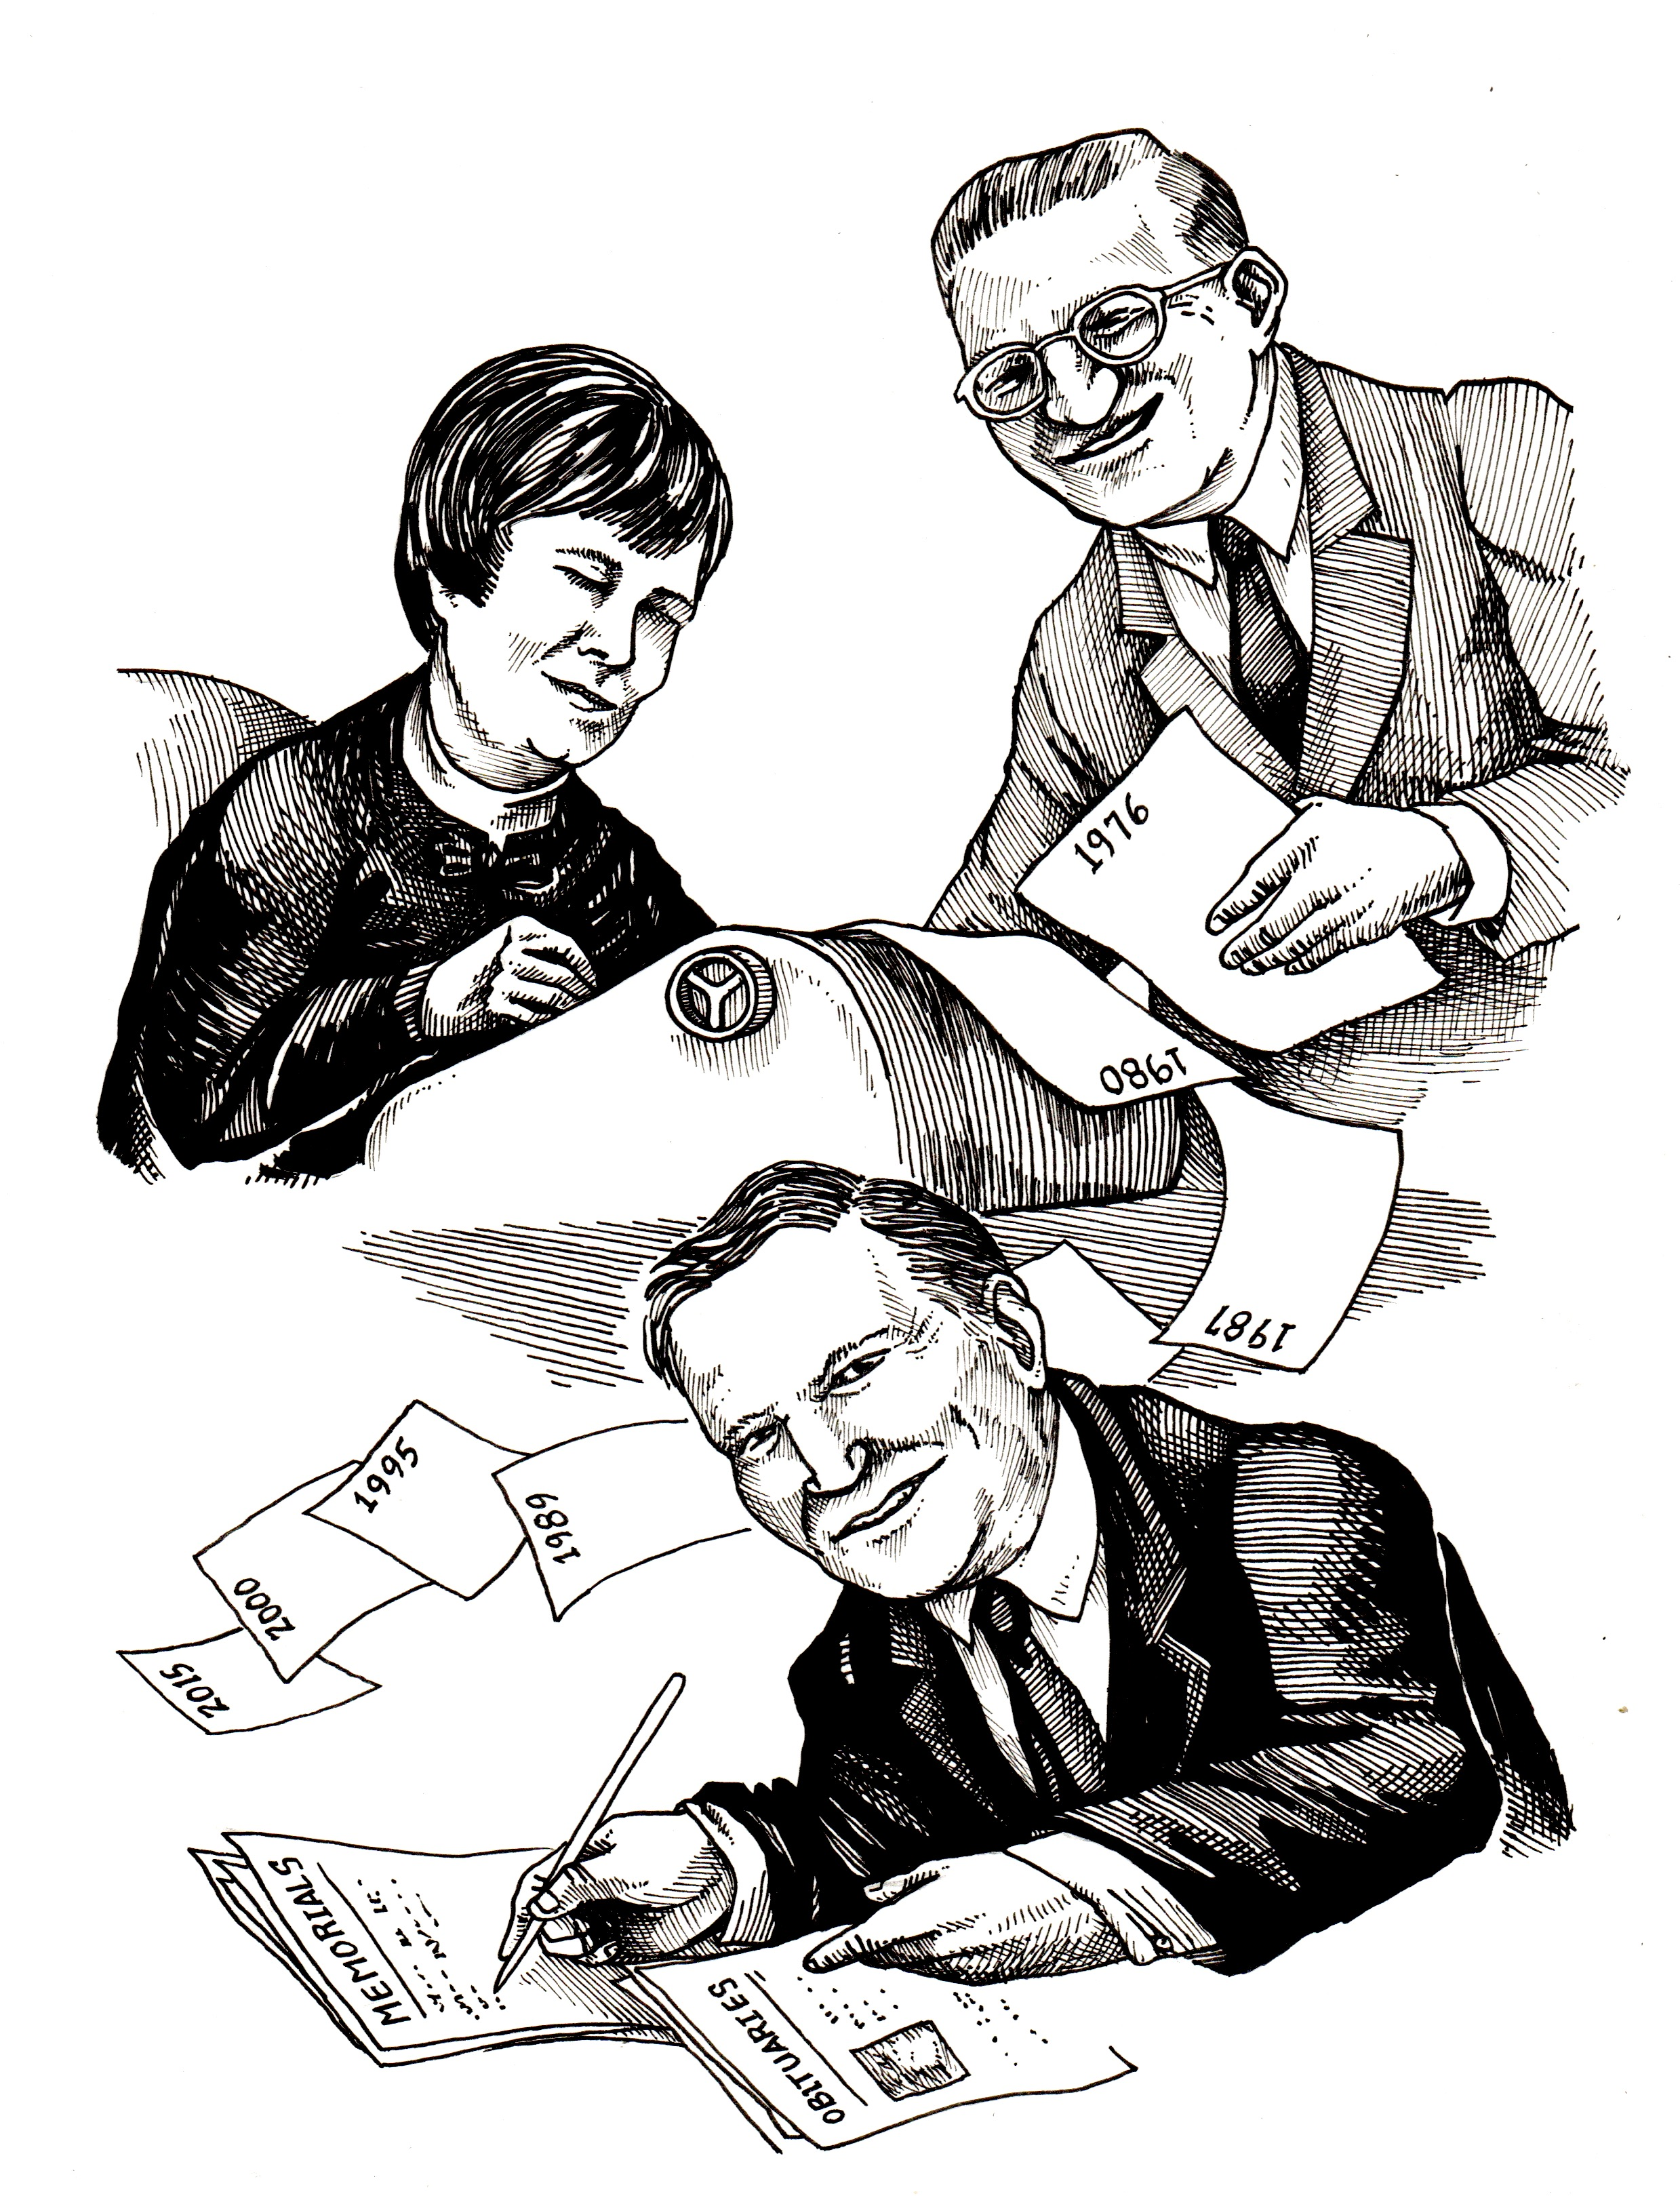
\includegraphics[width=0.6\linewidth,height=\textheight,keepaspectratio]{images/miu9.jpeg}

}

\caption{Harry G. Day (top), Elizabeth M. Greene (left), Donald J. Gray
(bottom)}

\end{figure}%

\epigraph{
The university traditionally upholds the ideal of human values in society. One would expect that the university, having had the benefit of the services of men and women at their peak, would retain them in their waning years. It is the totality of their service that should determine the reckoning.
}
{---Herman B Wells, \textit{Being Lucky: Reflections and Reminiscences}}

Universities, as human institutions, are composed of individuals who
occupy a variety of specific roles. Historically, they are composed of
three primary groups: students, teachers, and administrators. Each group
has characteristic duties, norms, and procedures that interact to
structure the institution in relation to its manifest goals of knowledge
creation, transfer, and preservation. The heart of the learning process
is the relation between teacher and student, with administrators playing
supporting roles to organize and facilitate learning.

Universities keep track of the members of their academic community with
bureaucratic procedures of admission and hiring, documentation of
advancement toward goals, and the commemoration of accomplishment. All
these activities produce written records, whether inscribed on paper,
photographically, or digitally.

For the past two centuries, Indiana University has retained a record of
each matriculated student and their progress toward a
diploma.\footnote{The IU Office of the Registrar is responsible. During
  the university's bicentennial, staff members began making some records
  public. See \href{https://first200.iu.edu/index.html}{``The First 200
  Degrees''} for biographical records of IU's first two hundred
  graduates.} The completion of degree requirements culminates in the
graduation ritual known as commencement. Former students, whether they
graduate or not, become members of the alumni body, which also maintains
records. In a similar fashion, a faculty records office keeps track of
the employment history of members of the academic staff. In contrast to
the limited time that students are working toward their degrees, the
faculty and administrative staff typically spend longer periods at the
university---often much longer. When faculty retire, they are usually
given the honorary designation ``professor emerita'' or ``professor
emeritus'' and feted at a ritual reception hosted by the administration
and attended by their colleagues.

Keeping such vital information has been a tortuous process, with natural
disasters and technological progress punctuating the history of archival
preservation as individual records accumulate. Two major fires---in 1854
and 1883---destroyed books and papers at the small campus. Library
collections were painstakingly rebuilt each time, but university records
and faculty papers were obliterated, leaving large gaps in institutional
archives for the nineteenth century.

Biography is essential to the writing of university history and
understanding the limitations of as well as opportunities provided by
different forms of archival preservation can be illuminating. Luckily,
the nineteenth-century institutional record was partially restored by
Theophilus Wylie's monumental work, discussed below.\footnote{Wylie,
  \citeproc{ref-wylie1890a}{\emph{Indiana University, Its History from
  1820, When Founded, to 1890, with Biographical Sketches of Its
  Presidents, Professor and Graduates, and a List of Its Students from
  1820 to 1887}}. See also Chapter~\ref{sec-three}.}

Like many aspects of IU's history, commemorative policy and practice can
be traced back to IU's ``second beginning'' in 1885, when the university
abandoned its original site on Seminary Square and moved across town to
establish the campus at Dunn's Woods. The proximate cause was an 1883
fire that destroyed Science Hall, one of the two main buildings. The
original campus was occupied for sixty years, from 1825 to 1885, and the
buildings had generic or functional names, such as the Seminary
Building, College Building, and Science Hall. The new campus was a
twenty-acre woodlot, purchased from the Dunn family, located on the
eastern edge of town. The trustees optimistically christened it
University Park.\footnote{\citeproc{ref-botm1884c}{Indiana University
  Board of Trustees, {``Minutes of the Board of Trustees of Indiana
  University, 04 June 1884--11 June 1884''}}.} But the new name did not
catch on, and reference to the relocated campus at ``Dunn's Woods''
endured, a harbinger of a shift in IU's naming practices to personal
names.

Bloomington, now numbering almost 3,500 residents, was coming into its
own as a city. It was featured prominently in an 1884 commercial
publication of county history, and IU was mentioned many times:

\begin{quote}
A detailed history of this university cannot be given in this volume;
neither can suitable or merited personal sketches be written of the many
eminent men {[}\emph{sic}{]} who have been connected with it, or have
gone as students from its halls to honored positions in almost every
State in the Union. It is appropriate, however, to say that the
institution has been the soul of Bloomington. A majority of the older
citizens are graduates or under-graduates, and their children and
grandchildren are now treading in their footsteps.\footnote{\citeproc{ref-blanchard1884a}{Blanchard,
  \emph{Counties of Morgan, Monroe, and Brown, Indiana}, 479}.}
\end{quote}

The city was being modernized, with new transportation options and more
municipal utilities available.

As city leaders of Bloomington heard about the planned relocation of the
IU campus to Dunn's Woods, they decided to honor one of the most
distinguished members of the faculty. In March 1884, Fifth Street was
renamed for Professor Daniel Kirkwood, a theoretical astronomer who
calculated regular intervals in the asteroid belt---the eponymous
``Kirkwood's gaps''---leading to the sobriquet ``the Kepler of
America.'' The \emph{Bloomington Telephone} reported:

\begin{quote}
Since the location of the new University buildings have been known, the
citizens, and especially those on 5th street, have been talking of
naming that thoroughfare Kirkwood Avenue, in honor of our distinguished
townsman, Prof.~Kirkwood. Last Friday night a petition was properly
presented to the Council, and by a vote the name was so changed. The new
University buildings now front on Kirkwood Avenue, if you
please.\footnote{{}. See also Edmondson,
  \citeproc{ref-edmondson2000a}{{``Daniel Kirkwood---{`{Dean} of
  American Astronomers'}''}}, p.~32, who mistakenly dated it as 1885.}
\end{quote}

Kirkwood, at the university since 1856, enjoyed an international
reputation for his scientific contributions. A popular teacher, he was
tolerant and indulgent in the classroom.

A couple of months later, the IU Board of Trustees decided to name the
new buildings---two of brick and one of wood---after esteemed university
figures. The larger brick edifice was named Wylie Hall, in memory of the
first president, Andrew Wylie, and in honor of Professor Theophilus
Wylie, who had taught for almost fifty years. The smaller brick
structure was named Owen Hall, to honor three distinguished brothers,
sons of Robert Owen of New Harmony, Indiana, fame, including retired
professor Richard Dale Owen, who had served on the faculty since
1864.\footnote{\citeproc{ref-botm1884c}{Indiana University Board of
  Trustees, {``Minutes of the Board of Trustees of Indiana University,
  04 June 1884--11 June 1884''}}.} The wood frame structure, serving as
the campus chapel and providing classrooms, was named after David
Maxwell, the first president of the board of trustees.\footnote{\citeproc{ref-botm1885b}{Indiana
  University Board of Trustees, {``Minutes of the Board of Trustees of
  Indiana University, 05 November 1885--11 November 1885''}
  (Bloomington, IN: Indiana University Archives; Indiana University
  Libraries Digital Collections Services, November 11, 1885),
  \url{https://purl.dlib.indiana.edu/iudl/archives/iubot/1885-11-05}}.}
These honorary namings inaugurated a tradition of recognizing
leaders---faculty, trustees, administrators---who had shaped the
university by inscribing their names on the new campus.

By the summer of 1888, the trustees ordered a roadway to be built
connecting the eastern end of Kirkwood Avenue to Wylie Hall, ``to be
covered with broken stone or broken stone and gravel.''\footnote{\citeproc{ref-botm1888a}{Indiana
  University Board of Trustees, {``Minutes of the Board of Trustees of
  Indiana University, 01 June 1888--07 June 1888''} (Bloomington, IN:
  Indiana University Archives; Indiana University Libraries Digital
  Collections Services, June 2, 1888),
  \url{https://purl.dlib.indiana.edu/iudl/archives/iubot/1888-06-01}}.}
Wide enough to allow two horse-drawn teams to pass, the road was near
the northern edge of the Dunn's Woods plot, leaving the bulk of the
property undeveloped. It also unintentionally confirmed the main
entrance to the new campus at Kirkwood and Indiana Avenues.

\section{Documenting the Academic
Community}\label{documenting-the-academic-community}

In 1881, the IU trustees asked Professor Theophilus Wylie to prepare a
historical catalog of the institution's history since its beginning in
1820.\footnote{Wylie was the seventh faculty member hired and had known
  all but three faculty before him---Baynard Hall, John Harney, and
  Ebenezer Elliott---who had left before his appointment in 1837. During
  his forty-nine years as a professor, he taught natural science and had
  stints of administrative work as librarian and acting president. He
  was personally acquainted with every IU faculty member until at least
  the 1880s (he died in 1895) as well as generations of university
  students.} After the 1883 fire consumed the previous three decades of
records, compounding the losses from an earlier fire in 1854, Wylie
turned to the living members of the IU community to salvage historical
information. He devised a questionnaire and embarked on extensive
correspondence by postal service. Painstakingly collating and organizing
reams of written responses, Wylie pressed on after his retirement in
1886. The resulting book, published in 1890, was a remarkably complete
biographical compendium of names of students, faculty, presidents, and
trustees, with some brief interpretive narratives interspersed. By
emphasizing biography, it underlined the importance of individuals
making up the academic community, forming a social institution. Wylie's
book, under the descriptive title \emph{Indiana University, Its History
from 1820, When Founded, to 1890, with Biographical Sketches of Its
Presidents, Professors and Graduates, and a List of Its Students from
1820 to 1887}, was long on a collective biography of the academic
community and short on a descriptive history of the university.

A decade and a half later, another contribution to IU history was
published, \emph{Indiana University, 1820--1904}, edited by history
professor Samuel B. Harding. It contained a historical sketch, an
analysis of curriculum development, and a bibliography of publications
of faculty and alumni.\footnote{\citeproc{ref-harding1904a}{Harding,
  \emph{Indiana University, 1820--1904}}.} For the first time, the
intellectual contributions of the entire IU professorate, both past and
present, were documented.

Nearly fifty years later, a different approach was taken in the
\emph{History of Indiana University, 1902--1937}, published in
1952.\footnote{Myers, \citeproc{ref-myers1952a}{\emph{History of Indiana
  University}, 1952}. Despite its title, the book had several chapters
  covering the entire history from 1820 to 1937.} Retired anatomy dean
Burton Myers studied IU faculty appointments from the beginning of
instruction to 1937, subdividing the chronology in half: 1824 to 1885
and 1885 to 1937. The choice of the dividing line was significant: the
beginning of the administration of President David Starr Jordan, who
represented a break from previous clerical leadership and the promotion
of a new spirit of research. Myers wrote, ``In contrast with the 60
appointments to the faculty in the first sixty-one years of the life of
the University, there were 897 appointments made in the fifty-two years
from 1885 to 1937.''\footnote{\citeproc{ref-myers1952a}{Myers, 577}.}
The rise in the number of faculty appointed was a consequence of the
growth of the student body over that 113-year span.\footnote{Myers,
  \citeproc{ref-myers1952a}{\emph{History of Indiana University}, 1952}.
  He included photographs of active faculty in 1937 who had served
  twenty-five years or more---fifty-two men and women in all.}

Myers's analysis was made possible by a new method of record-keeping
starting circa 1935: a cumulative collection of individual faculty data
collected on single sheets of paper. These biographical data sheets
contained information for each faculty member, such as name, title,
years of service, birth date and birthplace, educational background,
previous positions, marital status, and political and religious
affiliations.

Mellie P. Cravens, wife of John Cravens, IU registrar and secretary to
the board of trustees, worked in the Register of Graduates Office. In
1936, under her direction, a cumulative register of alumni between 1830
and 1935 was prepared.\footnote{Myers{}, pp.~479--480. Alumni records
  were transferred to the IU Archives in 1936. Before her marriage,
  Mellie had worked as a secretary for President Bryan. Myers{}, p.~593.}
Her husband, who served as President Bryan's trusted executive
assistant, retired in the summer of 1936 after forty-one years of
service. President Bryan, seventy-six years old, shocked the trustees by
indicating in early 1937 that he wanted to retire, after thirty-five
years at the helm. The trustees named Herman Wells, dean of the School
of Business Administration, acting president in June 1937, giving some
time to mount a proper search for a permanent replacement.\footnote{See
  Capshew, \citeproc{ref-capshew2012a}{\emph{Herman {B} Wells}}, Chapter
  5.} John Cravens died in August. Amid the flux of administrative
transitions, by November the trustees authorized Wells to support the
preparation of a faculty directory---a who's who of the instructional
staff---for use of the board and the administration.\footnote{\citeproc{ref-botm1937a}{Indiana
  University Board of Trustees, {``Minutes of the Board of Trustees of
  Indiana University, 22 November 1937--23 November 1937''}
  (Bloomington, IN: Indiana University Archives; Indiana University
  Libraries Digital Collections Services, November 23, 1937),
  \url{https://purl.dlib.indiana.edu/iudl/archives/iubot/1937-11-22}}.}
Thus, refinements in record management techniques allowed for recent
data to be integrated in cumulative reports of IU's academic community.

\section{Memorializing Faculty}\label{memorializing-faculty}

Although the board of trustees had noted faculty deaths occasionally in
their minutes with memorial resolutions, there was no regular policy. As
the faculty grew from a small, intimate group to a larger, more
heterogenous community, new president Wells suggested to the trustees
that memorial resolutions be prepared for faculty upon their death. The
trustees agreed with him, as noted in their 1940 minutes, but no
procedure was identified to produce them.\footnote{\citeproc{ref-botm1940b}{Indiana
  University Board of Trustees, {``Minutes of the Board of Trustees of
  Indiana University, 25 March 1940--26 March 1940''} (Bloomington:
  Indiana University Archives \& Indiana University Libraries Digital
  Collections Services, March 26, 1940),
  \url{https://purl.dlib.indiana.edu/iudl/archives/iubot/1940-03-25}}.}

Wells continued to report faculty deaths at the trustees' meetings
through the 1940s, but by the early 1950s, with increasing student
enrollments following the war and a concomitant swelling of faculty
numbers, the president instead created a necrology committee composed of
seasoned faculty members. The committee was responsible for ensuring
that a memorial resolution, usually written by departmental colleagues,
was prepared shortly after the death of a faculty member. That was the
plan, and most faculty were memorialized in this way. But a few faculty
fell inadvertently through the committee's net because the faculty that
had volunteered to write the resolution became too busy or forgot to
complete the assignment.

The first to chair the necrology committee was F. Lee Benns
(1889--1967), a member of the history faculty since 1920. A 1937 survey
indicated Benns was the most highly rated instructor among both faculty
and recent honors graduates. He was ``known as a very demanding teacher
but one widely revered.''\footnote{\citeproc{ref-madison2010a}{James H.
  Madison, \emph{Indiana University Department of History: Past to
  Present} (Bloomington: Indiana University Department of History,
  2010), 8}.} When Benns retired in 1954, Dean of the Faculties Herman
Briscoe wrote to John Stoner on President Wells's behalf, asking him to
take on the necrologist role.\footnote{\citeproc{ref-iu_faculty_necrology}{{``Faculty
  Necrology''} (Reference file, Indiana University Archives, n.d.)}.}
(Around this time, the role became known as the university necrologist.)
Stoner (1902--1988), a member of the Department of Political Science
since 1938, served as university necrologist for four years.\footnote{Stoner
  retired in 1972. His colleagues
  \href{https://purl.dlib.indiana.edu/iudl/archives/bfc/B21-1990}{memorialized
  him}, saying, ``His career spanned the transit from the insular
  elitism of the pre-war school with its few thousand students to the
  contemporary multiversity.''} Turning to another member of the history
department, in 1958 Wells recruited Associate Professor Chase Mooney
(1913--1973) to serve.\footnote{See
  \href{https://purl.dlib.indiana.edu/iudl/archives/bfc/B22-1974}{``MEMORIAL
  RESOLUTION ON THE DEATH OF CHASE C. MOONEY''}.}

Records documenting the history of the necrology committee in the 1960s
are lacking, but archival sources note that history professor Oscar
Winther (1903--1970) chaired the committee starting in 1964\footnote{See
  \href{https://purl.dlib.indiana.edu/iudl/archives/bfc/B22-1971}{``MEMORIAL
  RESOLUTION FOR OSCAR OSBURN WINTHER''}} and that folklorist John
Ashton (1900--1971), former dean of the graduate school, directed the
committee's work until 1970.\footnote{\href{https://purl.dlib.indiana.edu/iudl/archives/bfc/B35-1972}{Ashton's
  faculty memorial resolution} did not mention this role.} From 1970 to
1973, history professor Donald Carmony (1910--2005), editor of the
\emph{Indiana Magazine of History}, chaired the committee.

In 1973, President Ryan appointed chemistry professor Harry Day
(1906--2007) to the position of university necrologist. Day, a member of
the team that created the first fluoridated toothpaste in the 1950s, had
been at the university since 1940 and served various administrative
roles, including chemistry chair and associate dean for research and
advanced studies. Aided by his longtime secretary, Elizabeth Greene
(1921--2011), he conducted all aspects of his career with effectiveness
and dispatch. Although he retired in 1976, at seventy years of age, Day
continued as necrologist for sixteen years, until 1989. By the time he
reached eighty, Day appended an appeal to be relieved of his duties to
his annual necrology report.

Historical research occupied the energies of both Day and Greene into
the 1990s. Day embarked on a history of chemical instruction at IU,
dating back to 1837, when Theophilus Wylie was hired as a faculty member
in the natural sciences.\footnote{Wylie was a cousin of Andrew Wylie,
  the first president, who died in 1851.} Not only was chemistry a
venerable subject of teaching, but the department had also grown to be
the largest among the science departments at IU. In the course of his
research, Day discovered the existence of Wylie's extensive personal
diaries in the university archives. The diaries gave details about
Wylie's activities during the greater part of the nineteenth century,
including his family life and university events, often with an
indication of his personal reactions. Greene laboriously transcribed the
faded handwriting into typescript. Archivist Dolores Lahrman
(1920--1997) and her staff assisted in translating the frequent Greek,
Latin, and French phrases that Wylie used to express his meaning.

The transcription of the diaries was completed in 1987, with Greene
providing a preface and Day supplying an introduction. Wylie's diaries
became an invaluable source for both Bloomington and IU history of the
last two-thirds of the nineteenth century. Later, staff at the IU
Archives discovered some missing diaries, and Greene dutifully
transcribed those too, completing the work in 1992.\footnote{See
  \href{https://archives.iu.edu/catalog/InU-Ar-VAA1230}{archival
  description of Theophilus Wylie's diaries}.} The same year, Day
published his historical chronicle, entitled \emph{The Development of
Chemistry at Indiana University, 1829--1991}.\footnote{\citeproc{ref-day1992a}{Harry
  G. Day, \emph{The Development of Chemistry at Indiana University,
  1829--1991} (Bloomington: Indiana University, 1992)}.} Nearly seven
hundred pages, it was a meticulous compendium of names, dates, and facts
about every aspect of teaching and research in the discipline as it was
practiced at the university.

In 1989, Day's importuning about a replacement yielded fruit, as
President Tom Ehrlich appointed English professor Donald Gray (b. 1927)
as university necrologist. Gray, a specialist in Victorian literature,
joined the English faculty in 1956. He was a superb teacher, supervising
dozens of Ph.D.~dissertation students, and a noted editor, publishing
the Norton \emph{Pride and Prejudice} and \emph{Alice in Wonderland} as
well as serving as editor of the academic journals \emph{College
English} and \emph{Victorian Studies}. He also edited and contributed to
\emph{The Department of English at Indiana University Bloomington,
1868--1970}, published in 1973, following the observance of the IU
sesquicentennial in 1970.\footnote{\citeproc{ref-gray1973a}{Donald J.
  Gray, ed., \emph{The Department of English at Indiana University
  Bloomington, 1868--1970} (Bloomington: Indiana University, 1973)}.}

Gray had witnessed the university's growth and diversification for a
third of a century upon his appointment and had extensive contacts in
the faculty and administration. The new job meant increased exchanges
with every school on the Bloomington campus plus coordinating
information from other campuses from around the state. Gray was quietly
effective, working with faculty colleagues as they crafted memorial
sketches of their late peers, often supplying insights to their
personalities and their impact on university life.

Once written, faculty memorial resolutions were read aloud at meetings
of the Bloomington Faculty Council (BFC), co-chaired by the BFC
president and the campus's presiding officer, first the Bloomington
chancellor and more recently the Bloomington provost. In 2010, education
professor Robert Arnove questioned ``the process by which memorial
resolutions are prepared and brought before this body'' because ``a
number of colleagues have passed away in 2008 and 2009 and I haven't
seen anything for them.'' Vice Provost for Faculty and Academic Affairs
Thomas Gieryn explained:

\begin{quote}
We've worked very, very hard---``we'' being Don Gray, the campus
necrologist and emeriti faculty members and I---have worked hard
contacting deans and chairs of all the departments to provide memorial
resolutions. We beg them, we give them models, we tell them it's not
that onerous. It gets difficult sometimes and I noticed certainly as you
did that sometimes it takes a great deal of time to find the right
person to write the resolution. We encourage all colleagues who know of
someone who has died who has not had a memorial resolution read to bring
that to the attention of their chair so that we can reach that
closure.\footnote{\citeproc{ref-bfcm2010a}{Indiana University
  Bloomington Faculty Council, {``Indiana University Bloomington Faculty
  Council Minutes, 07 September 2010''} (Bloomington: Indiana University
  Archives \& Indiana University Libraries Digital Collections Services,
  September 7, 2010),
  \url{https://purl.dlib.indiana.edu/iudl/archives/bfc/2010-09-07}}.}
\end{quote}

To be sure, a few deceased faculty members escaped the necrologist's
net, but this unique historical record grew year upon year, providing
informed summations of faculty careers and a symbolic closure to
university service.

Professor Gray soldiered on as university necrologist for decade after
decade, cajoling faculty writers and editing their prose, on every
campus of the university. Over time, however, as campus autonomy grew in
Indianapolis and in the regionals and administrative personnel changed,
the other campuses stopped sending information about faculty deaths. By
the time she left office in 2011, Provost Karen Hanson suggested Gray's
title be changed to IUB necrologist. In 2017, after twenty-eight years,
he penned a short memo, ``The IU Necrologist: Duties and Procedures,''
based on his experience, and submitted a request to the university
administration to be relieved of this duty.\footnote{\citeproc{ref-gray2017a}{Donald
  J. Gray, {``The IU Necrologist: Duties and Procedures''} (circa
  2017)}.}

Gray got his wish the following year. He was now ninety years old and in
his sixty-second year of service at Indiana University. In February
2018, Provost Lauren Robel presented a verbal encomium at a regular
meeting of the BFC, right after the customary reading of the latest
faculty memorial resolution. She prefaced her remarks with a verse of
Victorian poet laureate Alfred, Lord Tennyson, from his famous poem,
\emph{In Memoriam A.H.H.}:

\begin{quote}
I sing to him that rests below,\\
And, since the grasses round me wave,\\
I take the grasses of the grave,\\
And make them pipes whereon to blow.
\end{quote}

She began her tribute to Gray by noting, ``We start every meeting of the
Bloomington Faculty Council with our memorial resolutions. And it is
extraordinarily fitting that we do so. The resolutions are human and
charming and grounding and give us a sense of our history and our
colleagues, and the vast range of the interest represented on this
campus.'' She continued by introducing Gray and commending his work as
the university necrologist.

Robel remarked that Gray was a leading scholar of Victorian literature,
thus her choice of Tennyson's elegy, musing that his scholarship might
have motivated his nearly thirty years of service as necrologist, ``or
perhaps it was simply his love for Indiana University and his
understanding of the importance of this role.'' Regardless, ``Don has
done incredibly important work'' for his university colleagues, for the
campus, and for the family and friends of departed faculty
members.\footnote{\citeproc{ref-iubfc2018a}{Indiana University
  Bloomington Faculty Council, {``Ndiana University Bloomington Faculty
  Council Minutes, 06 February 2018''} (Bloomington: Indiana University
  Archives \& Indiana University Libraries Digital Collections Services,
  February 6, 2018),
  \url{https://purl.dlib.indiana.edu/iudl/archives/bfc/2018-02-06}}.}

Gray turned his files on university necrology over to the Office of the
Vice Provost for Faculty and Academic Affairs during the 2017--18
academic year. Indermohan Virk, a staff member responsible for the
Patten Foundation lecture series, added the role of campus necrologist
to her portfolio. In her duties, she works with the leadership of BFC
and colleagues of deceased faculty to craft an appropriate memorial
resolution, which is read into the record during regular council
meetings.

\section{The Bicentennial Era}\label{the-bicentennial-era-1}

Amid his long service as necrologist, Gray embarked on a collateral
project to collect video interviews of emeriti professors. Begun in
2005, it was a way to collect stories of faculty experiences from
retired academics. Similar in concept to the oral history center,
initiated in 1970 as part of the university's sesquicentennial
commemoration, it gathered personal narratives of faculty careers. In
2008, it was folded into the Bicentennial Oral History Project to
capture alumni recollections in advance of the 2020 institutional
anniversary. Teachers and students contributed vital data to this
ongoing effort. Gray expressed the rationale of the emeriti project:
``What we were trying to get, I think, is a picture of what a faculty
member did, how it changed and how the students changed.''\footnote{\href{https://mediaschool.indiana.edu/news-events/news/item.html?n=brownlee-preserves-stories-of-emeriti-faculty}{``Brownlee
  preserves stories of emeriti faculty''}} By 2017, Gray had conducted
150 interviews and bequeathed the project to two other emeriti
professors, Bonnie Brownlee and Bruce Jaffee, both younger.\footnote{See
  also
  \href{https://web.archive.org/web/20230413202919/https://200.iu.edu/doc/IU-bicentennial-final.pdf}{\emph{Indiana
  University Bicentennial Final Report}} (Bloomington: Indiana
  University, 2020), 30--31.}

The Office of the Bicentennial was created in 2016 to plan, coordinate,
and implement a wide array of public events to shed light on the history
of Indiana University, culminating in the institution's 200th
anniversary on January 20, 2020.\footnote{A good overview is provided in
  the \emph{Indiana University Bicentennial Final Report}.} Special
attention was paid to documenting the history of students, faculty,
administrators, and alumni. Staff at the Office of the Registrar helped
with statistical analyses of the historical demography of the student
body, providing estimates of the total number of individuals taking at
least one course since the beginning of instruction in 1825 (nearly
2,000,000) and the count of graduates (approaching 1,000,000). A website
featuring biographical profiles of the first 200 graduates was produced,
and then coverage was extended to all degree recipients.\footnote{\href{https://allgrads.indiana.edu/}{The
  Degree Compendium} and \href{https://first200.iu.edu/}{The First 200}}
In a similar fashion, the faculty records group within the Office of the
Vice Provost for Faculty and Academic Affairs provided data on the
number and characteristics of instructional staff since classes began in
1825. Because of historical changes in the definition of faculty as well
as incomplete records, they could only give a ballpark estimate, which
was near 50,000. In contrast, because of the smaller numbers of trustees
and officers, the administration has proven easier to document its
historical demography. The Office of the Bicentennial chose to continue
a long-running series of volumes of biographical sketches that stretched
back to Theophilus Wylie's 1890 IU history. The result was
\emph{Trustees and Officers of Indiana University, Volume III:
1982--2018}, with a team of five editors and numerous contributors. The
historical total of trustees and officers was about 650
individuals.\footnote{Linda Fariss Keith Buckley Derek F. DiMatteo and
  Colleen Pauwels, eds., \citeproc{ref-buckley2019a}{\emph{Trustees and
  Officers of Indiana University, Volume III: 1982--2018} (Bloomington:
  Indiana University, 2019)}. The first historical list is found in
  Wylie, \citeproc{ref-wylie1890a}{\emph{Indiana University, Its History
  from 1820, When Founded, to 1890, with Biographical Sketches of Its
  Presidents, Professor and Graduates, and a List of Its Students from
  1820 to 1887}}; earlier volumes were Myers,
  \citeproc{ref-myers1951a}{\emph{Trustees and Officers of Indiana
  University 1820--1950}, 1951} and Eleanor Roehr,
  \citeproc{ref-roehr1983a}{\emph{Trustees and Officers of Indiana
  University, 1950 to 1982} (Bloomington: Indiana University, 1983)}.}

As a human institution, it remains important to document the members of
the academic community and their activities. The first history of
Indiana University, published in 1890, was a successful attempt to
reconstruct the names and careers of individual members of the bodies of
students, faculty, and administrators of the institution's first seven
decades in the face of incomplete historical data. By 1900, the office
of the registrar was established and had devised a system to track each
student who matriculated and those who graduated. As enrollments grew,
the number of graduates increased, and the alumni association
established a collateral tracking system as it underwent
professionalization in the first quarter of the twentieth
century.\footnote{See Shirley, \citeproc{ref-shirley2004a}{\emph{The
  Indiana University Alumni Association}}.} By 1935, administrators had
rationalized faculty recordkeeping, facilitating administrative
reporting and historical documentation. Although the media and
techniques of recordkeeping have changed over time, maintaining accurate
and complete records of each member of the academic community continues
to be a core aspect of IU's identity and makes possible historical
analysis, reflection, and celebration.

\bookmarksetup{startatroot}

\chapter{The Resurrection of Wylie House}\label{sec-ten}

\begin{figure}[H]

{\centering 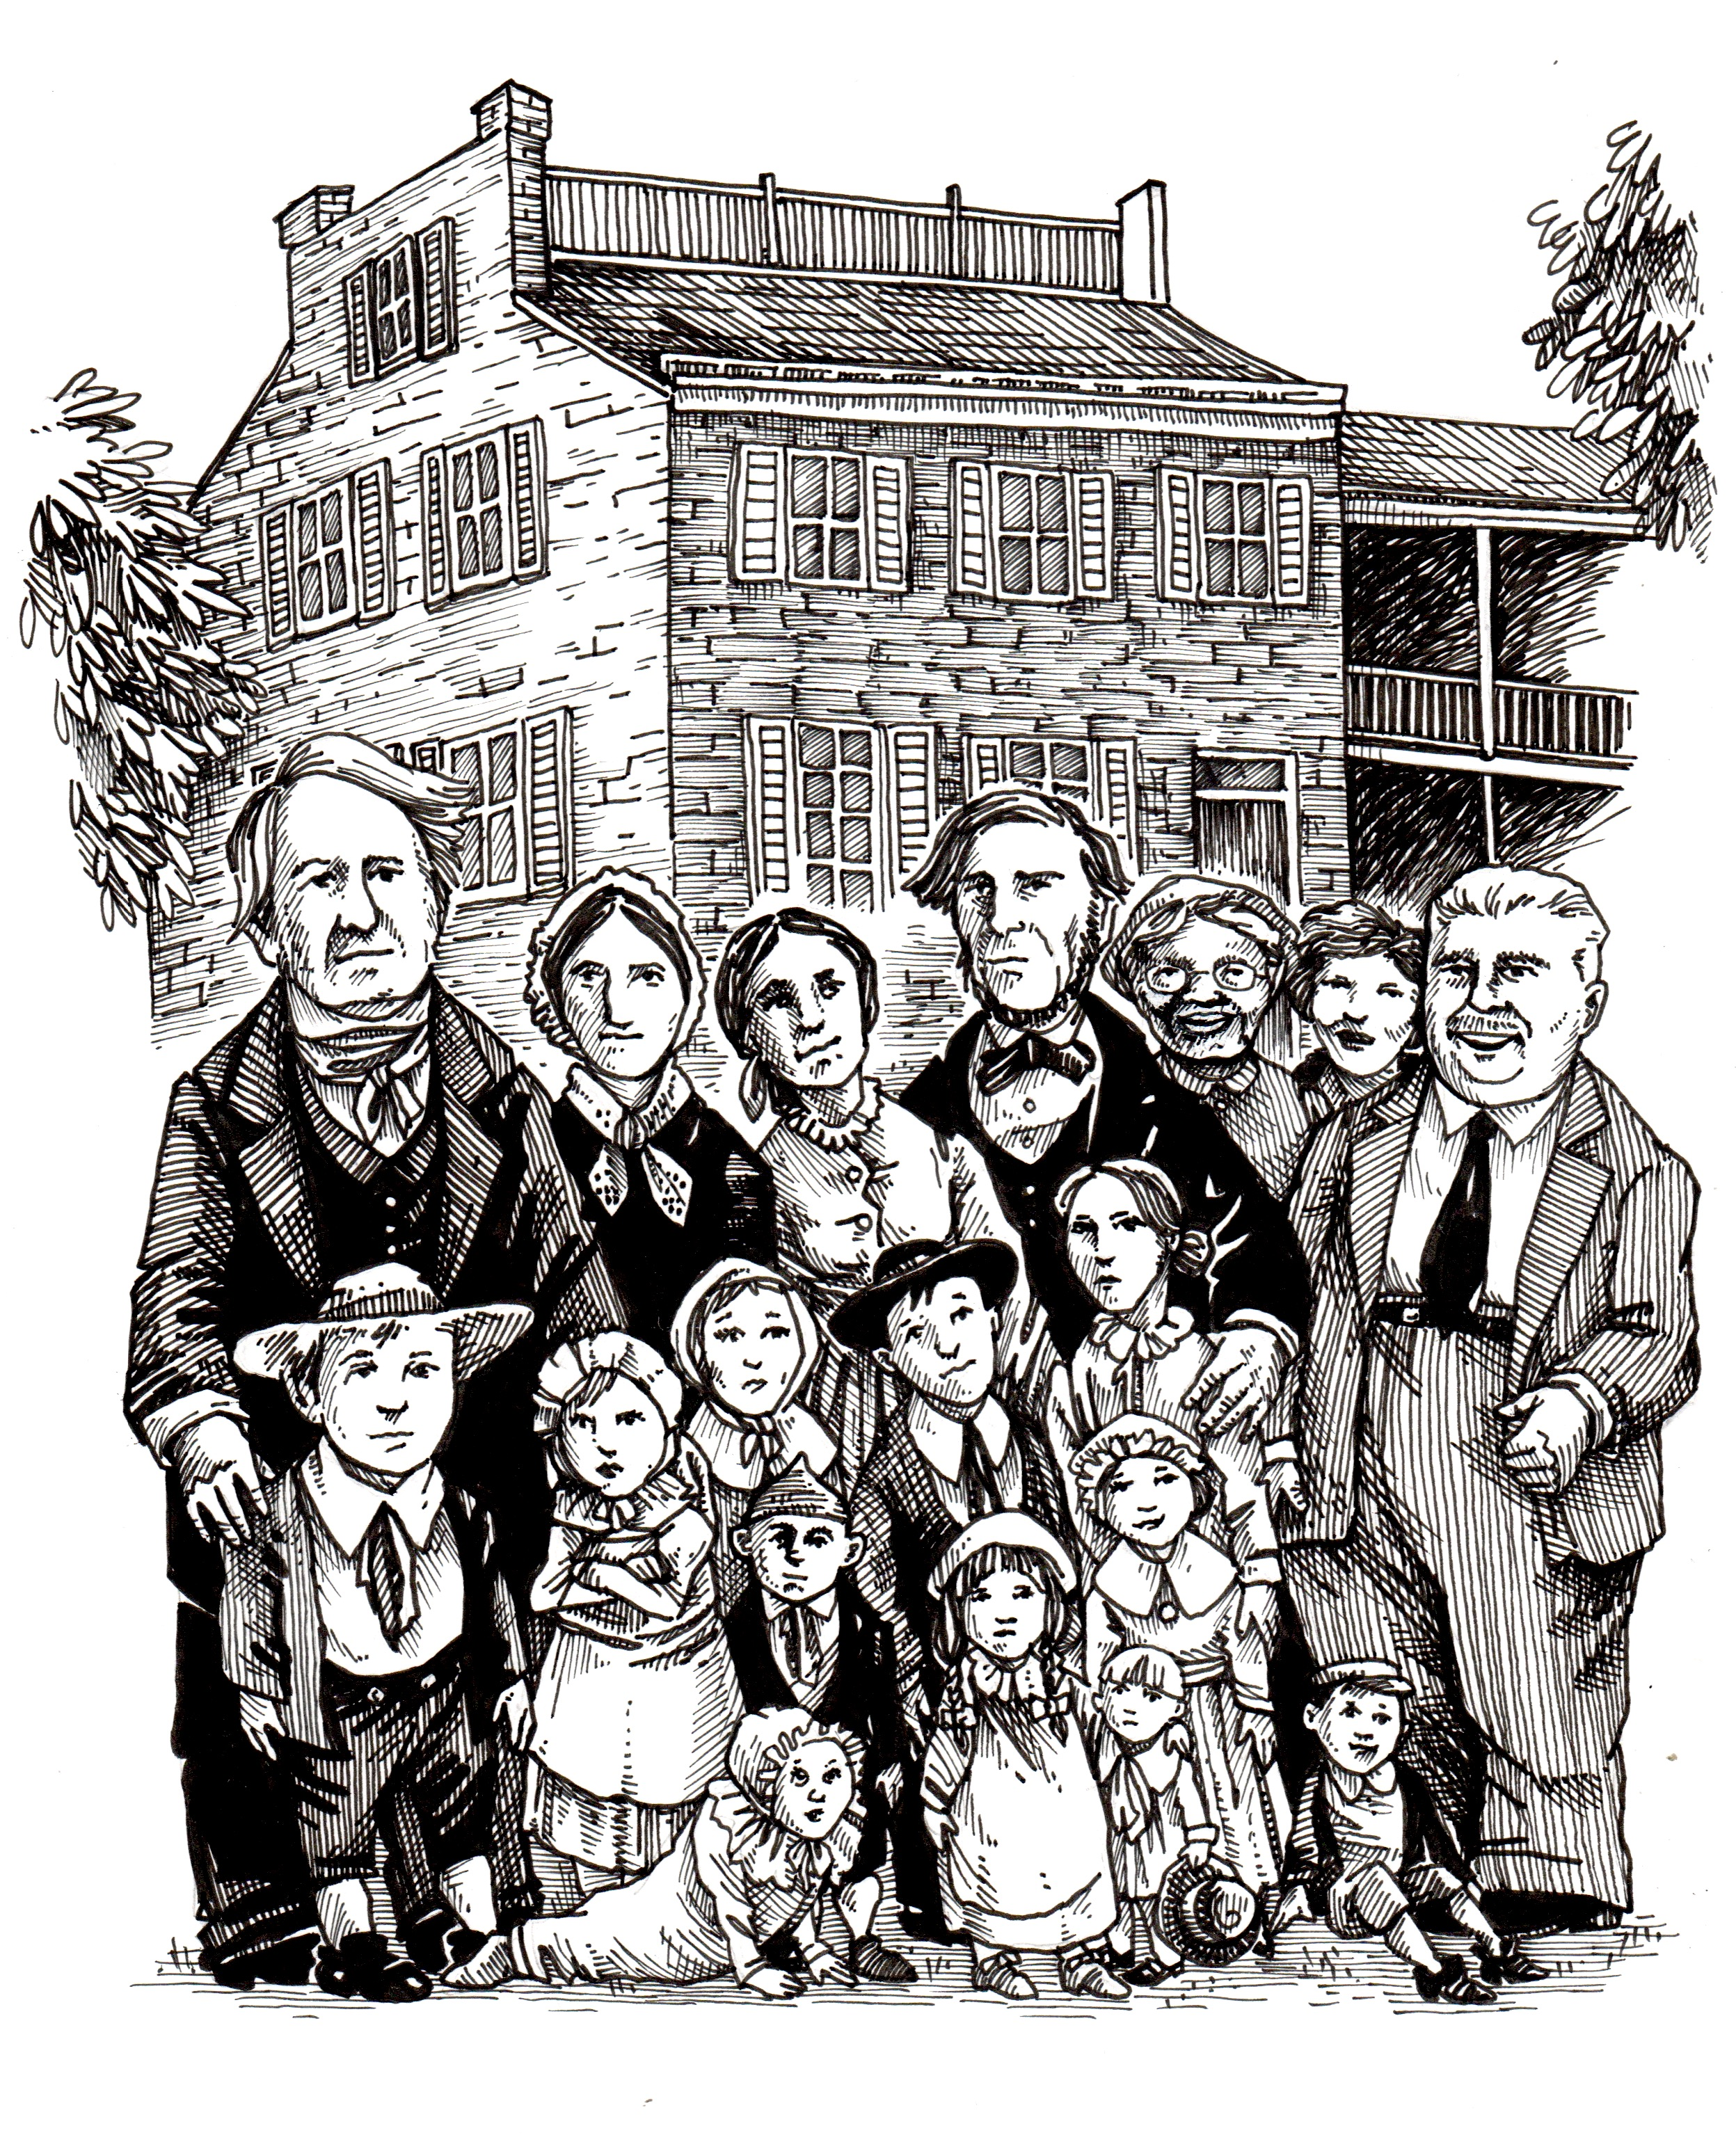
\includegraphics[width=0.6\linewidth,height=\textheight,keepaspectratio]{images/miu10.jpeg}

}

\caption[Wylie House]{Wylie House. Back row, l-r: Andrew Wylie, Margaret
Wylie, Rebecca Wylie, Theophilus Wylie, Lizzie Breckenridge, Lilian
Hershey, and Herman Wells. Front row: Wylie children.}

\end{figure}%

\epigraph{
I was always interested in anything that was a living reminder of the antiquity of the University.  
}
{---Herman B Wells, Interview}

What is the most significant surviving physical artifact from the early
history of Indiana University? A handful of early diplomas, handwritten
letters, and published materials form a sparse but invaluable
documentary record. No physical trace remains of the university's first
campus building---only an Indiana state historical marker stands on the
site where IU began as the Indiana State Seminary in the 1820s. One
possible candidate is the 1843 book \emph{The New Purchase; or, Seven
and a Half Years in the Far West}, which offers the first extended
narrative about IU, written by its inaugural professor, Baynard Hall.

In terms of material culture as well as on programmatic grounds, a
strong case can be made for the Wylie House, built in 1835 by the first
IU president, Andrew Wylie, as a residence for his large family.
Purchased by the university in 1947, it started functioning as a museum
twenty years later but did not employ its first curator until 1983. Now,
as the Wylie House Museum, it plays a central role in IU's history and
heritage activities.

When the house was built in 1835, the institution was known as Indiana
College, and classes had been offered for a decade. Wylie had been in
office for seven years, and student enrollment had reached forty.
Located two blocks from campus, at Second and Lincoln Streets, the house
was one of the finest in the area. Built of brick in the Georgian style,
the house sat on a crest of land, surrounded by twenty acres, including
cultivated gardens, tree plots, and outbuildings.

President Wylie guided the institution for twenty-two years until a
woodchopping accident led to his death by infection in 1851. The house
remained in his immediate family until 1859, when it was sold to
Professor Theophilus A. Wylie, a half-cousin of Andrew Wylie, who also
had a large family. That Wylie family stayed in the home for over fifty
years, a period that encompassed the Civil War to the Great War. In
1915, the house was sold to IU political science professor Amos S.
Hershey and his wife, Lillian S. Hershey. They owned the house for over
thirty years, until it was sold to Indiana University in 1947. President
Herman B Wells engineered its purchase, taking an important step in
preserving the property and laying the groundwork for its eventual use
as a historic house museum. Wells's historical sensibility had been
nurtured years before, starting with his involvement with another old
house in Bloomington.

\section{Living at Woodburn House}\label{living-at-woodburn-house}

In 1932, after a couple of years as an instructor in economics at
Indiana University, Herman Wells started renting rooms at the Woodburn
House, 519 North College Avenue. The young teacher, thirty years old,
had an interest in antique furniture and was beginning to collect
English fox-hunting prints, befitting his status as a confirmed
bachelor. The landlord was IU history professor emeritus James A.
Woodburn, who had been living in Ann Arbor since his retirement in 1924,
the same year Wells received his Bachelor of Science degree from the
School of Commerce and Finance. Woodburn, who had lived in the family
house since his 1856 birth, had a keen appreciation for its long
history.

The house, built in 1829, was a historic structure. In 1855, his father,
also an IU professor, James W. Woodburn, purchased the entire block for
\$1,100 and added a second story to the house in 1858. After the death
of the father James in 1865, his widow took in student boarders. Their
daughter, Ida Woodburn, hosted the first official meeting of the Delta
chapter of the Kappa Kappa Gamma sorority there in 1873. Local lore
suggested that an infamous ``bogus'' underground student newspaper,
\emph{The Dagger}, was started there. Later, IU faculty members,
including psychologist William Bryan and political scientist Amos
Hershey, resided in the house. The son James inherited the house and
raised a family there.\footnote{\citeproc{ref-dagger}{{``The Dagger:
  1875--80''} (Bloomington: Indiana University Archives, n.d.).
  Reference file, Indiana University Archives};
  \href{https://wiki.kkg.org/index.php/Delta\#The_Early_Years}{``Delta:
  The Early Years''};
  \href{https://bloomingpedia.org/wiki/Woodburn_House}{``Woodburn
  House''}}

Wells enjoyed living in the Woodburn House and its proximity to campus.
He also became acquainted with another historic house in this
period---the Wylie House---which was located a half dozen blocks south
of the Woodburn House. In 1915, the house had passed from the Wylie
family to another IU professor, Amos Hershey, and his wife, Lillian.

Amos S. Hershey, a scion of the Pennsylvania chocolate manufacturing
family, joined the Indiana faculty in 1895. A specialist in
international law and diplomacy, in 1914, he was the founding chair of
the Department of Political Science.\footnote{\citeproc{ref-field1952a}{Oliver
  P. Field, \emph{Political Science at Indiana University, 1829--1951}
  (Bloomington: Bureau of Government Research, Department of Government,
  Indiana University, 1952)}.} After the First World War, President
Woodrow Wilson appointed him to the US delegation to the Paris Peace
Conference as a technical advisor. Lillian, a proficient singer, wed
Amos in 1892. She was an active businesswoman, selling antiques and home
furnishings from her residence, which she called The Old Treasure House.
The Hersheys entertained often, and Wells was a frequent guest. Calling
Mrs.~Hershey ``a delightful person,'' Wells recalled, ``Everybody knew
the Hersheys. The house was most interesting, because she just lived
with her antiques. She'd sell anything she had---rugs and furniture and
so forth. The house was the perfect setting for that.''\footnote{\citeproc{ref-wells1992a}{Herman
  B Wells, {``Oral History Interview by Bonnie Williams''} (Wylie House
  Collections, March 19, 1992)}.} Their friendship was fueled by a
shared interest in antiques and fine furnishings. Professor Hershey
retired from teaching in 1932 and died the following year. Lillian
Hershey continued to live in the Wylie House and operate her antiques
business.

In 1933, Wells took a leave of absence to serve the state of Indiana as
it reorganized its financial institutions during the Depression. A
banking wunderkind, he analyzed the banking system in Indiana and
supervised a team that rewrote the state's banking laws in early 1933.
The reform legislation passed under the governorship of Paul McNutt,
former dean of the IU School of Law, creating a new Indiana Department
of Financial Institutions. Wells served in three capacities: as
secretary to the Commission on Financial Institutions, bank supervisor,
and supervisor of the Division of Research and Statistics for the
department. This triple role gave him great authority in regulating the
state's banking system---and a comfortable salary to indulge his taste
for antiques and fine furnishings.\footnote{See Wells,
  \citeproc{ref-wells1980a}{\emph{Being Lucky}}, Chapter 4; and Capshew,
  \citeproc{ref-capshew2012a}{\emph{Herman {B} Wells}}, Chapter 3.}

In 1935, Wells moved from teaching to administration when he was
appointed dean of the IU School of Business Administration by President
William Bryan. He continued his meteoric administrative rise two years
later, when the board of trustees selected him as acting president after
Bryan retired after thirty-five years. Wells was in office for only a
few weeks when he noticed that Lillian Hershey had put the Wylie House
on the real estate market, and he began a warm correspondence with
her.\footnote{\citeproc{ref-hershey}{{``Hershey, Mrs. Amos Shartle''}
  (Bloomington, IN: Indiana University Archives, n.d.).
  IUA/C213/B268/F}.} At the August 1937 meeting of the trustee board,
acting president Wells reported to the trustees that the Wylie House was
for sale, listed at \$30,000. Further discussion by the board was
planned but apparently not memorialized.\footnote{\citeproc{ref-botm1937b}{Indiana
  University Board of Trustees, {``Minutes of the Board of Trustees of
  Indiana University, 09 August 1937''} (Bloomington, IN: Indiana
  University Archives; Indiana University Libraries Digital Collections
  Services, August 9, 1937),
  \url{https://purl.dlib.indiana.edu/iudl/archives/iubot/1937-08-09}}.}
Wells continued to serve as acting president for nine months, fulfilling
day-to-day responsibilities as well as launching an ambitious university
self-study, before being named the eleventh IU president in March
1938.\footnote{\citeproc{ref-capshew2012a}{Capshew, \emph{Herman {B}
  Wells}, chap. 5}.}

\section{Paying Tribute to Andrew
Wylie}\label{paying-tribute-to-andrew-wylie}

Two months later, in May 1938, the new president received a letter from
Roy Quinn, an Indianapolis resident, lamenting the neglect of the first
president, Andrew Wylie, on the recent Foundation Day, a celebration of
the university's heritage. Ruing that he was not a ``University man''
despite his rearing in Bloomington, Quinn admitted, ``I learned to love
old I.U. and revel in its glorious past and pull for its promising
future.'' He observed that, over the half century he had been visiting
Bloomington's Rose Hill Cemetery, he had never seen a flower on Wylie's
grave. He suggested, ``With a band and military units and everything
else needed to make such a thing a success why not lay a wreath upon the
grave of the original `forgotten man'?''\footnote{\citeproc{ref-quinn1938a}{Roy
  Quinn, {``Letter to Herman Wells''} (Indiana University Archives, May
  16, 1938). IUA/C213/B455}.}

In his reply, Wells agreed that the university should pay tribute to
Wylie and suggested that a committee of the senior class place a wreath
on his grave each Foundation Day. ``This would cause students to
remember Dr.~Wylie,'' he thought, ``more than any other action I can
think of.''\footnote{\citeproc{ref-wells1938a}{Herman B Wells, {``Letter
  to Roy Quinn''} (Indiana University Archives, May 26, 1938).
  IUA/C213/B455}.} The next year, Wells oversaw an expansion of the 1939
Foundation Day commemoration, with activities not just in Bloomington
but also around Indiana (Kokomo, Marion, Anderson, Terre Haute, Fort
Wayne, North Vernon, Michigan City, Rushville, Muncie, Washington,
Decatur, Peru, Spencer, South Bend, Evansville, and Salem) and in other
states (St.~Louis, St.~Petersburg, Boston, Champaign, Iowa City, Denver,
Grand Rapids, Louisville, Los Angeles, Milwaukee, New Haven, and
Detroit).\footnote{\citeproc{ref-indynews1939a}{{``{I.U.} Founding to Be
  Observed by Alumni Throughout the World,''} \emph{Indianapolis News},
  May 2, 1939, 13}.}

Wells wrote to Quinn again, telling him that a pilgrimage to the
gravesite of Andrew Wylie was planned as part of the Foundation Day
activities and inviting him to come. ``These services mark the
fulfillment of an idea you had a year ago this month,'' Wells wrote,
``and I hope they may become a part of Indiana University's tradition
for all the years to come.''\footnote{\citeproc{ref-wells1939a}{Herman B
  Wells, {``Letter to Roy Quinn''} (Indiana University Archives, May 2,
  1939). IUA/C213/B455. IUA/Reference file: Foundation Day}.}
Demonstrating Wells's ability to harness an unexpected suggestion into a
university priority, the Wylie pilgrimage was the first stirring of a
new tradition.\footnote{\citeproc{ref-indystar1939a}{{``Inaugurating
  What Is Expected to Be an Annual Custom,''} \emph{Indianapolis Star},
  May 5, 1939, 17. Photo caption}. Pictured: Albert Higdon, president of
  the senior class; Herman Wells; Mrs.~Harry A. Axtell, granddaughter of
  President Wylie; Miss Madeline, great-granddaughter of President
  Wylie; William Bryan.}

The tradition became an annual event, continuing throughout the war
years (with one exception in 1944). President emeritus Bryan was a
frequent participant along with President Wells and student leaders. In
1945, the 125th anniversary of the university was celebrated at
graduation ceremonies, and the commencement speaker, Ralph Cooper
Hutchison, president of Washington and Jefferson College, attended the
pilgrimage and laid the wreath on Wylie's grave. (Wylie had been
president of both colleges sequentially before coming to IU, and in
1816, he unsuccessfully attempted to merge them.)\footnote{Before he
  assumed the IU presidency, Andrew Wylie was president of both
  Jefferson College and Washington College, located a dozen miles apart.
  He attempted unsuccessfully to merge them in 1816; they were united in
  1865.} For the decade after the war, the pilgrimage remained a part of
the celebration of the university's founding, known as Founders Day
after 1951.\footnote{Pilgrimage records are spotty; no documents have
  surfaced for 1946 and 1948.}

\section{The Purchase of Wylie House}\label{the-purchase-of-wylie-house}

During the war, the director of the university library, Robert Miller,
put together an ad hoc archives committee to preserve and care for
documentation of the university's past.\footnote{\citeproc{ref-iua_c213_b30}{(Bloomington:
  Indiana University Archives, n.d.). IUA/C213/B30/F}.} The president's
suite in Bryan Hall, constructed in 1936, was built with a five-floor
archival unit attached, called the President's File Room. It contained a
vast collection of documents generated during the thirty-five-year
administration of former president Bryan as well as copies of past
official catalogs, bulletins, and printed announcements and programs.
Wells, aware of the need for good recordkeeping, acceded to the plan to
rename the space the University Archives and put librarian Mary Craig in
charge. His secretaries kept his presidential files in good order. A
sign was posted in the room:

\begin{quote}
NOTICE!\\
No person shall take any paper of any sort from this room without giving
a receipt therefor to the file clerk, who is made directly responsible
to the Trustees of the University. This order applies to all persons,
including the undersigned.\\
HERMAN B WELLS
\end{quote}

The notice humorously underscored Wells's egalitarian convictions.

After the Second World War ended in 1945, Wells kept his eye on the
Wylie House and continued his correspondence with Lillian Hershey,
sharing their interest in antiques and decorative objects. The president
was still living in the Woodburn House and found it was well suited for
entertaining and other official functions. (James Woodburn had given the
house to IU in 1941, two years before his death.)\footnote{\citeproc{ref-botm1941c}{Indiana
  University Board of Trustees, {``Minutes of the Board of Trustees of
  Indiana University, 10 October 1941--11 October 1941''} (Bloomington,
  IN: Indiana University Archives; Indiana University Libraries Digital
  Collections Services, October 10, 1941),
  \url{https://purl.dlib.indiana.edu/iudl/archives/iubot/1941-10-10}}.}

Wells used the opportunity of a postwar visit by Governor Ralph Gates in
1947 to put into motion an ingenious plan. On a tour around campus and
the city, Wells and Gates drove by the Wylie House. The governor was
suitably impressed and urged Wells to put the funds to acquire the
property on the university's 1947 budget request.\footnote{Clark,
  \citeproc{ref-clark1977a}{\emph{Indiana University}, 1977}, p.~150,
  180--181. See also Wells, \citeproc{ref-wells1992a}{{``Oral History
  Interview by Bonnie Williams''}}.} The purchase went through, and
Wylie House became an institutional property after 112 years of service
as a family home. The terms included a provision for Mrs.~Hershey to
live in the house four years without paying rent or taxes. When she
moved to Florida in 1951, the university took possession.\footnote{\citeproc{ref-botm1947c}{Indiana
  University Board of Trustees, {``Minutes of the Board of Trustees of
  Indiana University, 12 June 1947--14 June 1947''} (Bloomington, IN:
  Indiana University Archives; Indiana University Libraries Digital
  Collections Services, June 12--14, 1947),
  \url{https://purl.dlib.indiana.edu/iudl/archives/iubot/1947-06-13}};
  \citeproc{ref-botm1947d}{Indiana University Board of Trustees,
  {``Minutes of the Board of Trustees of Indiana University, 30 June
  1947''} (Bloomington, IN: Indiana University Archives; Indiana
  University Libraries Digital Collections Services, June 30, 1947),
  \url{https://purl.dlib.indiana.edu/iudl/archives/iubot/1947-06-30}};
  \citeproc{ref-capshew2012a}{Capshew, \emph{Herman {B} Wells},
  184--85}.}

University archivist Craig, who had received a Master of Library Science
degree from Columbia University, turned out to be less interested in the
written record than in the material culture of the past, and she soon
added to her responsibilities the role of unofficial but acknowledged
caretaker of the Wylie House. Both Wells and Craig were aficionados of
antique furniture and historic houses, and the prospect of furnishing
the Wylie House in period pieces was enticing to each. In their quest
for antiques, Wells and Craig used campus storage spaces, including the
attic of Wylie House, to hold accumulating treasures of furniture and
other furnishings.

In October 1951, two grandchildren of Theophilus Wylie joined the
trustee board for lunch: sister and brother, Mrs.~Morton Bradley (née
Marie Boisen), from Boston, and Mr.~Anton Boisen, from Chicago. They
provided valuable background information about the house and some of its
former occupants. Also, family letters, receipts, and other documents
were conveyed to the University Archives. Soon after, the trustees
discussed four options for the Wylie House:

\begin{quote}
\begin{itemize}
\tightlist
\item
  Establish the house as a museum, to depict in detail how a scholar of
  the 1830's lived, worked, and entertained. Much of the original
  furniture is available, and we know exactly where it was placed.
\item
  Restore the house as it was, or in the style of the period, with some
  additional comforts, and use as a guest house. It would be
  incorporated into either the Halls of Residence or the Union system.
  Such usage is common in other universities.
\item
  Restore the house structurally and use it for headquarters for some
  group such as the Alumni Association.
\item
  Restore the house structurally and use it as one of the home
  management houses.\footnote{\citeproc{ref-botm1951a}{Indiana
    University Board of Trustees, {``Minutes of the Board of Trustees of
    Indiana University, 16 November 1951''} (Bloomington, IN: Indiana
    University Archives; Indiana University Libraries Digital
    Collections Services, November 16, 1951),
    \url{https://purl.dlib.indiana.edu/iudl/archives/iubot/1951-11-16}}.}
\end{itemize}
\end{quote}

Although the board favored the guest house option, action was deferred.
In 1953, with university office space at a premium, Wylie House was
pressed into service as the temporary headquarters of IU Press, launched
in 1950.\footnote{\citeproc{ref-botm1952a}{Indiana University Board of
  Trustees, {``Minutes of the Board of Trustees of Indiana University,
  01 December 1952''} (Bloomington, IN: Indiana University Archives;
  Indiana University Libraries Digital Collections Services, December 1,
  1952),
  \url{https://purl.dlib.indiana.edu/iudl/archives/iubot/1952-12-01}};
  \citeproc{ref-capshew2012a}{Capshew, \emph{Herman {B} Wells}, 185,
  203--4}.} The university press office stayed in the building until
1959. Craig corresponded with another grandson, T. A. Wylie, at the end
of 1954 and early 1955, sending him a Wylie family tree and exchanging
other information.

\section{Remembering Andrew Wylie}\label{remembering-andrew-wylie}

Although Wells was familiar with the first president's house and had
engineered its purchase for the university, Andrew Wylie the man and his
influence on IU were a mystery. In the spring of 1960, after announcing
his impending retirement two years hence, Wells renewed his attention to
the house associated with the original campus at Second Street and
College Avenue. In support of the idea that the house should be restored
to its original appearance, he further publicized the legacy of Andrew
Wylie.

In November 1960, Wells gave a speech at Louisville's Filson Club, a
venerable history society dedicated to Kentucky and the Ohio River
valley. The speech was published in the club's history quarterly under
the title ``The Early History of Indiana University as Reflected in the
Administration of Andrew Wylie, 1829--1851,'' under Wells's byline. He
claimed that Wylie, almost forgotten outside of IU circles, was a
``notably important figure in the early development of western state
universities.'' The more he knew about Wylie, the more determined he
became to bring Wylie's legacy to light.

With the aid of IU archivists and historians, Wells pieced together his
narrative account from the few surviving sources, including contemporary
reminiscences from peers and students, to portray Wylie's personality
and career as an educator. He summed up his contributions under four
categories: establishing the curriculum, promoting good student-faculty
relations, serving as chief spokesman for higher education, and mounting
successful defenses of the university against outside forces.\footnote{\citeproc{ref-capshew2012a}{Capshew,
  \emph{Herman {B} Wells}, 121--22}.} Wells concluded with a salute to
his predecessor:

\begin{quote}
If the Indiana University of today is an institution of immeasurable
value and service to the state and nation, and I firmly believe that it
is, we must revere the memory of the first president who offered the
intellectual and moral leadership so vital and necessary to the
University in its infant days. He gave stability in a period
characterized by instability. A university is a durable institution,
built on the accumulated wisdom of the past. How fortunate that our past
included Andrew Wylie!\footnote{\citeproc{ref-capshew2012a}{Capshew,
  \emph{Herman {B} Wells}, 126}.}
\end{quote}

By the time Wells's article appeared in print in 1962, the Wylie House
restoration was underway.\footnote{\citeproc{ref-wells1962a}{Herman G.
  {[}sic{]} Wells, {``The Early History of Indiana University as
  Reflected in the Administration of Andrew Wylie, 1829--1851,''}
  \emph{Filson Club Historical Quarterly} 36 (1962): 113--27}.}

Andrew Wylie's legacy was emerging as a touchstone for the university's
past, and his home was a material embodiment of that legacy. It was a
visible sign of the university's rich cultural heritage, and its
curation and interpretation would provide varied ways to connect to IU's
history.

\section{Wylie House Restoration}\label{wylie-house-restoration}

The Edward D. James architectural firm was selected to perform the
long-delayed renovation of the Wylie residence and produced a condition
report for the university in late 1960. The project was termed a
``restoration,'' which meant renovating the structure to resemble its
original finished appearance in 1835.

Architect Edward James had experience in historic preservation and, in
1957, was appointed American Institute of Architects (AIA) preservation
officer for the state of Indiana, where he coordinated the Historic
American Building Survey Inventory. His younger associate, H. Roll
McLaughlin, was assigned as project architect for the Wylie House
restoration. In 1960, McLaughlin was appointed AIA assistant
preservation officer, working under James. Later that year, McLaughlin
was elected first vice president of the new Historic Landmarks
Foundation of Indiana (now Indiana Landmarks), a nonprofit organization
formed by civic and business leaders interested in the preservation of
architectural heritage.\footnote{Among the leaders of Historic Landmarks
  Foundation of Indiana were Eli Lilly and Herman Krannert. H. Roll
  McLaughlin, \citeproc{ref-mclaughlin1983a}{{``HABS in Indiana,
  1955--1982: Recollections,''} in \emph{Historic American Buildings
  Survey in Indiana}, ed. T. M. Slade (Bloomington: Indiana University
  Press, 1983), 13--20}, pp.~16--17.} Drafting plans for the Wylie House
restoration, McLaughlin embarked on an important early project at the
outset of his long career.\footnote{\citeproc{ref-wyliehouse2001a}{Preservation
  Development Inc., {``Wylie House Historic Structure Report''}
  (Bloomington, 2001)}.}

McLaughlin relied on his architectural training and understanding of the
principles of historic preservation to guide the project. In the fall of
1960, McLaughlin spent ten weeks in Europe studying preservation
techniques and stopped by Washington, Pennsylvania, where Andrew Wylie
lived prior to coming to Bloomington.\footnote{\citeproc{ref-wyliehouse2001a}{Preservation
  Development Inc., 15}.} (Nationwide design standards were not
instituted until 1966, when the National Historic Preservation Act was
passed.) Motivated by a sense of original intent, he focused narrowly on
the architectural creation of the house in 1835 rather than considering
the entire eighty-year span during which two related, yet separate Wylie
families were in residence. The goal was to restore the house to the
year it was built.

The IU trustee board approved an agreement with the Edward D. James firm
in January 1961, with a preliminary cost budget of \$250,000, with a
justification: ``Because of the nature of the work, which precludes
definite advance plans and specifications, this will be done on a
time-card basis cost of work done.''\footnote{\citeproc{ref-botm1961b}{Indiana
  University Board of Trustees, {``Minutes of the Board of Trustees of
  Indiana University, 20 January 1961--21 January 1961''} (Bloomington,
  IN: Indiana University Archives; Indiana University Libraries Digital
  Collections Services, January 20--21, 1961),
  \url{https://purl.dlib.indiana.edu/iudl/archives/iubot/1961-01-20}}.}
In June 1961, President Wells appointed a Committee on the Restoration
of Wylie House, chaired by Joseph Franklin, longtime IU treasurer, and
including archivist Mary Craig, physical plant director H. H. Brooks,
librarian Cecil Byrd, landscape architect Frits Loonsten, and architect
Edward James.\footnote{\citeproc{ref-wyliehouse2001a}{Preservation
  Development Inc., {``Wylie House Historic Structure Report,''}
  13--14}.}

The actual renovation work was done by IU physical plant employees,
around fifteen in all, supervised by John Dixon, a master carpenter. The
initial phase, lasting about a year, stabilized the foundation, rebuilt
the west wall, repointed all exterior walls, rebuilt fireplace hearths,
removed the roof, and removed plaster from interior walls. For the next
three years, a variety of finish work occurred. A new roof, with poplar
shake shingles split by physical plant employee Wally Sullivan, was
installed, and copper guttering was added. Interior walls were re-lathed
and replastered. In the kitchen, the floor joists were replaced and the
floorboards too, with old-growth poplar flooring. The back porch,
including its foundation, was removed. Wood trim was stripped and
repainted, exterior doors and some windowsills were replaced, new
limestone steps were installed at entrances, and most windows were
reglazed with antique glass. The attic was reconstructed, with new
walls, doors, stairs to the roof, and a roof access hatch with copper
hinges. The main staircase was carefully disassembled, stripped of
paint, reassembled, and repainted.\footnote{\citeproc{ref-wyliehouse2001a}{Preservation
  Development Inc., 14--15}.}

As the restoration project continued, in 1962, the university got a new
president, Elvis J. Stahr, and Herman Wells moved into the role of
university chancellor, a new senior administrative post. The traditional
pilgrimage to Wylie's grave in Rose Hill Cemetery on Founders Day went
on, now led by President Stahr and joined regularly by Wells.

\section{Wylie House Museum}\label{wylie-house-museum}

Indiana University issued a press release announcing the opening of the
museum to the public in October 1965. It fell to the university
archivist, Mary Craig, to keep the place running. With no additional
staff and little interpretation, by default the museum focused on the
building itself in its renovated state. After the initial flurry of
publicity, the museum was open by appointment. Craig continued to
acquire period furnishings, and those that were not put on display
immediately were consigned to storage at the university. There was
little attempt to curate the history of the house as successive families
lived there. There was, however, a trove of documents slowly gathering
in the archives, through occasional gifts and the rediscovery of
materials already in the archives that had been poorly cataloged
previously.

Preceding the 1967 pilgrimage to Wylie's gravesite, President Stahr led
a special Founders Day ceremony to commemorate the centennial of the
admission of women to IU. A total of six women received honorary
degrees. Then Stahr invited the audience to join him and Wells for

\begin{quote}
a pilgrimage to the grave and then to the house of Andrew Wylie, first
president of Indiana University. Wylie House was purchased for the
University at the express request of Governor Ralph Gates, who
instructed that it be restored to its original form. The necessity of
collecting funds for the renovation and the time required to do the
actual work postponed the opening until two years ago. Since then,
increasing numbers of students, parents, school children, and others
have toured this home of so much historical significance to Indiana
University and to the State. I should add, Wylie House gives some
\emph{continuing reality} to our annual Founders' Day reminder that ours
is a pioneer university.
\end{quote}

Charter bus transportation was available from the Indiana Memorial
Union.\footnote{\citeproc{ref-stahr1967a}{Elvis Stahr, {``Founders' Day
  Ceremonial''} (Indiana University Archives, May 3, 1967),
  \url{http://fedora.dlib.indiana.edu/fedora/get/iudl:2078062/OVERVIEW}.
  IUA/C75}.}

During the 1970 IU sesquicentennial year, records indicate that an
application for nomination of the Wylie House to the National Register
of Historic Places was begun by IU staff but not completed.\footnote{\citeproc{ref-wyliehouse2001a}{Preservation
  Development Inc., {``Wylie House Historic Structure Report,''} 16}.}
In 1972, Chancellor Wells bought a neighboring house as a real estate
investment to protect Wylie House and help buffer possible future
development.\footnote{The address was 215 E. Second Street. Indiana
  University Board of Trustees, \citeproc{ref-botm1972a}{{``Minutes of
  the Board of Trustees of Indiana University, 22 September 1972''}
  (Bloomington, IN: Indiana University Archives; Indiana University
  Libraries Digital Collections Services, September 22, 1972),
  \url{https://purl.dlib.indiana.edu/iudl/archives/iubot/1972-09-22}}.}
In 1976, the United States bicentennial brought renewed attention to
local landmarks, including several historic structures in Bloomington
connected to the university. A flurry of successful listings on the
National Register of Historic Places was completed, including the Monroe
County Courthouse (1976) and the Carnegie Library (1978).\footnote{Dana
  D'Esopo, co-chair of the Historic Preservation Subcommittee filled out
  the
  \href{https://npgallery.nps.gov/NRHP/GetAsset/36d693e4-5c6b-4f6d-bed4-75e20051adc4}{courthouse
  form}; Bruce Tone and Dana D'Esopo, Save the Library Committee, filled
  out the
  \href{https://npgallery.nps.gov/NRHP/GetAsset/af4df484-de1d-40bf-9b65-ab846ed02b43}{library
  form}.} Three properties with strong links to IU were listed: the
Wylie House (1977), Seminary Square Park (1977), and the Old Crescent
(1980).\footnote{Donald Carmony, IU professor of history and editor of
  the Indiana Magazine of History, and H. Roll McLaughlin, restoration
  architect, filled out the
  \href{https://npgallery.nps.gov/NRHP/GetAsset/02688528-9112-4793-a0ec-9871bda0d52c}{form
  for the Wylie House}; Mary Alice Gray of the Bloomington/Monroe County
  Bicentennial Commission for
  \href{https://npgallery.nps.gov/NRHP/GetAsset/f7982d4d-3546-47c9-8afc-ae2cba1025eb}{Seminary
  Square}; and Daniel F. Harrington of the IU Heritage Committee for the
  \href{https://npgallery.nps.gov/NRHP/GetAsset/696439ba-d253-4034-a2c4-214caa9e038f}{Old
  Crescent}.} Coincidentally, Mary Craig retired in 1977, but she
remained active. In 1978, the home next door was purchased by the
university, dubbed the Wylie House Annex, and provided office space and
additional storage.\footnote{\citeproc{ref-wyliehouse2001a}{Preservation
  Development Inc., {``Wylie House Historic Structure Report,''} 21}.}

In the third volume of Thomas Clark's massive sesquicentennial history
of IU, he mentioned the Wylie House in passing, calling it an
``institutional shrine'' to the university's past and a ``memorial of
`Andrew the First.'\,''\footnote{\citeproc{ref-clark1977a}{Clark,
  \emph{Indiana University}, 1977, 181, 512}.} The vision that animated
the restoration of the house's architectural glory in the 1960s had
dissipated in the 1970s, and Wylie House remained an architectural
relic, impassively witnessing the passing years.

\section{Curatorial Beginnings}\label{curatorial-beginnings}

The annual pilgrimage to Andrew Wylie's gravesite and to the Wylie House
had continued, with President John Ryan leading the party in 1983. The
home, Ryan noted, ``was a mansion almost beyond comprehension'' in its
day.\footnote{\citeproc{ref-botm1983a}{Indiana University Board of
  Trustees, {``Minutes of the Board of Trustees of Indiana University,
  09 April 1983''} (Bloomington, IN: Indiana University Archives;
  Indiana University Libraries Digital Collections Services, April 9,
  1983),
  \url{https://purl.dlib.indiana.edu/iudl/archives/iubot/1983-04-09}}.}
That year, Bonnie Williams was hired as the first curator of Wylie
House. With determination and energy, Williams launched into making the
house more than an architectural relic.

Williams, who was the only staff member at the Wylie House, did have a
small group of volunteers who helped with research and visitor relations
and interpretation. For the first few years, the house had limited
public hours, and, in her words, ``interpretation was confined to
standard third-person tours describing the collection and giving some
historical background about the Wylie family and early Indiana
University.''\footnote{\citeproc{ref-williams1996a}{Bonnie Williams,
  {``Playing in the Stream of History: A Flexible Approach to
  First-Person Interpretation,''} \emph{Association for Living
  Historical Farms and Agricultural Museums Proceedings} 14 (1996):
  255--61}.}

In 1991, one volunteer, who had worked previously as a first-person
interpreter at another historic site, was eager to try first-person
techniques at the Wylie House. Williams was skeptical about whether
there was enough research into the Wylie family and their daily life to
support the creation of a living-history character, as well as how to
deal with certain anachronistic features of the house, such as
electrical outlets and a security system.

After more reading and discussion, however, Williams was willing to try
it. Using a ``my time / your time'' approach, Williams was inspired to
create a first-person ``ghost interpretation.'' The idea was that the
character worked ``in the context of a recreated past but could call on
a knowledge of past and future events as needed to help explain the
story to visitors.''\footnote{\citeproc{ref-williams1996a}{Williams,
  256}.} Williams, dressed in the style of the 1840s, greeted fourth
graders who were on a field trip to the historic house:

\begin{quote}
Good morning and welcome to all of you! Mrs.~Williams, who looks after
Wylie House, told me she was expecting a group of young visitors this
morning. She thought you might enjoy it if I showed you the house and
told you a little about what it was like when I was a girl here. I said
I'd be most pleased to do so. I enjoy talking about old times. Of
course, 150 years is a long time to remember back! But I will say, my
memory has always been sharp. My name is Elizabeth Wylie. You may call
me Miss Wylie. Andrew Wylie was my Papy, and this is the home I grew up
in many, many years ago. Oh, my dears, what memories.\ldots{} Let's go
into the parlor where we can sit and visit for a spell.\footnote{{\citeproc{ref-williams1996a}{{``Playing
  in the Stream of History''}}.}, p.~255. See also Stacy Flora Roth,
  Past into Present: Effective Techniques for First-Person Historical
  Interpretation (Chapel Hill: University of North Carolina Press,
  1988), where Williams's technique is discussed on page 17.}
\end{quote}

Williams explained the rationale behind the approach: ``Instead of
transporting visitors back in time and pretending it is the 1840s, I
bring someone from the 1840s into the present---a `ghost,' so to
speak.''\footnote{\citeproc{ref-williams1996a}{255}.}

By playing a ghost, the interpreter had access to knowledge about the
past as well as the present, providing flexibility in answering
questions about the house or its furnishings. Even obvious anachronisms,
such as the motion detectors for the security system, could be
explained. The ghost of Miss Wylie answered when a schoolchild pointed
out the small plastic box with a blinking red light in the corner of a
room:

\begin{quote}
You know, I studied on that for the longest time. It certainly wasn't
here when I was a girl. Finally I asked Mrs.~Williams and she told me it
was a burglar alarm! I told her that when I was a girl, our ``burglar
alarm'' was our dog! Well, in those days there was always someone in the
house, and nowadays that's not so, and we don't have a dog here anymore
to protect the house. So I suppose it is a good idea to have one of
these new burglar alarms, just to be on the safe side.\footnote{\citeproc{ref-williams1996a}{258}.}
\end{quote}

Williams admitted that the ghost approach necessitated a lot of
background research to be able to respond to visitors' observations and
to answer questions, but in the end, ``we talk about what we do
know.''\footnote{\citeproc{ref-williams1996a}{259}.} At the end of the
group tour, Williams came out of character: ``As you know, I am not
really a ghost. I am an historian. It's my job to learn about the past
and to share what I've learned with you. And I have found that sometimes
the best way to do that is to pretend, like we did today. I enjoyed
sharing and learning with you! Do you like studying history this way?
Maybe someday some of you will become historians, and you may even do
work like this!''\footnote{\citeproc{ref-williams1996a}{258}.} Both
children and adults responded well to this conclusion, which gave the
tour a sense of closure and provided the opportunity to ask questions
about the museum.

Williams used and refined her ghost interpretation at the Wylie House
for nearly a decade for visitor tours. She also practiced a form of
historical reenactment, where a small group would get into character as
various members of the Wylie family and read their nineteenth-century
letters to each other.

In the 1990s, some house features needed additional remediation. In
1994, the trustee board officially renamed the facility the Wylie House
Museum, to better reflect its function.\footnote{\citeproc{ref-botm1994a}{Indiana
  University Board of Trustees, {``Minutes of the Board of Trustees of
  Indiana University, 24 September 1994''} (Bloomington, IN: Indiana
  University Archives; Indiana University Libraries Digital Collections
  Services, September 24, 1994),
  \url{https://purl.dlib.indiana.edu/iudl/archives/iubot/1994-09-24}}.}
In 1995, a wheelchair ramp was installed, which required excavation on
the north side. Some artifacts were found, mostly bits of broken china,
and cleaned and cataloged. Another conservation assessment survey was
completed in 1995.

In 1995, volunteer researcher Elaine Herold, aided by curator Williams,
published a compilation of 163 letters exchanged by the members of the
Andrew Wylie family. The project was made possible by an Indiana
Heritage Research Grant from the Indiana Historical Society and the
Indiana Humanities Council. Under the title \emph{Affectionately Yours:
The Andrew Wylie Family Letters, 1828 to 1859}, the book gives glimpses
of the mid-nineteenth-century Hoosier life of the first family of
IU.\footnote{\citeproc{ref-williams1995a}{Bonnie Williams and Elaine
  Herold, eds., \emph{Affectionately Yours: The Andrew Wylie Family
  Letters, 1828 to 1859} (Bloomington: Indiana University Wylie House
  Museum, 1995)}.} The letters reveal information about travel, weather,
and academic life, as well as family drama and emotion about courtship
and marriage, sickness and death. By showing the rich texture of
day-to-day living, the collection of letters humanizes the Wylie family
as they faced the perennial challenges of life.

An eighteenth-century fortepiano surfaced in IU storage in 1997, having
lain there for decades. Curator Williams and the Wylie House Museum
volunteers were excited, thinking that it might be the one that Andrew
Wylie brought to Bloomington in 1829. Despite extensive research, the
fortepiano's provenance was murky. It likely belonged to the Wylies but
could not be proven conclusively. In any event, plans were made to
restore the instrument, built in 1795 by the Broadwood Company in
England. Local harpsichord craftsman Theodore Robertson rebuilt the
instrument. Based on a bibliography of the Wylies' own sheet music,
musicians searched the Lilly Library for appropriate period music ``that
represents what the Wylie family would likely have experienced.'' In
2001, an audio recording, \emph{Wylie House Music from the Parlor}, was
produced, played on the Broadwood fortepiano and featuring two pianists
and two vocalists.\footnote{\citeproc{ref-wyliehouse2001b}{{``Wylie
  House Music from the Parlor,''} 2001. Audio recording; liner notes by
  Sophia Grace Travis}.}

With funds provided by state and federal grants, Williams started
preparing a bibliography of Andrew Wylie with the aid of stalwart
volunteers. Published in November 2000, \emph{Andrew Wylie: A
Bibliography} was edited by Diane Chaudemanche and Elaine Herold. It
contained an annotated list of seventy-three primary, secondary, and
tertiary sources, plus a short list of artifacts associated with Wylie,
including the house.\footnote{\citeproc{ref-chaudemanche2000a}{Diane
  Chaudemanche and Elaine Herold, eds., \emph{Andrew Wylie: A
  Bibliography}, 2000, \url{http://hdl.handle.net/2022/20329}}.}

\section{Jo Burgess and the Education
Center}\label{jo-burgess-and-the-education-center}

Jo Burgess, former head of Preservation Services at IU Libraries, became
the director of the Wylie House Museum at the beginning of the 2000--01
academic year.\footnote{\citeproc{ref-botm2000a}{Indiana University
  Board of Trustees, {``Minutes of the Board of Trustees of Indiana
  University, 15 September 2000''} (Bloomington, IN: Indiana University
  Archives; Indiana University Libraries Digital Collections Services,
  September 15, 2000),
  \url{https://purl.dlib.indiana.edu/iudl/archives/iubot/2000-09-15}}.}
She had a knack for physical artifacts and an aesthetic that was
historically informed. In her first year, a consultant produced a
thorough analysis of the house's history and current state of
preservation.\footnote{\citeproc{ref-wyliehouse2001a}{Preservation
  Development Inc., {``Wylie House Historic Structure Report''}}.} The
\emph{Wylie House Historic Structure Report} made sober reading, with
several serious threats to the house's historical fabric identified.
Next door, the Wylie House Annex had had substantial structural issues
ever since it was acquired that made it nearly impossible to control
environmental conditions.

In her first years, Burgess had the white walls decorated with
historically appropriate colors, embellished by artful stencil work. She
compiled an index to the family letters contained in
\emph{Affectionately Yours} and published a second edition in 2002.
After that, an unexpected trove of more letters was acquired by the
Wylie House Museum, consisting of several hundred from the Theophilus
Wylie family and another one hundred letters from the Andrew Wylie
family. Several letters found their way into the third edition of the
book, published in 2011.\footnote{\citeproc{ref-burgess2011a}{Jo
  Burgess, ed., \emph{Affectionately Yours: The Andrew Wylie Family
  Letters}, I: 1828--1859, II: 1860--1918 vols. (Bloomington: Wylie
  House Museum, 2011). Volume I:
  \url{https://scholarworks.iu.edu/dspace/items/4323e65e-8053-4624-a19c-cec3c14205f0};
  Volume II:
  \url{https://scholarworks.iu.edu/dspace/items/4c56273e-06d6-427e-a533-769e9cf5504e}}.}

Burgess made concerted efforts to expand educational programming. In
summer 2005, she hired a full-time curator of education---Bridget
Edwards---who had a doctorate in anthropology.\footnote{Edwards served
  from July 2005 to September 2011.}

Aided by the dean of university libraries Suzanne Thorin, Edwards got on
the radar of the university administration in 2006, when the trustees
heard a brief presentation by Vice President Clapacs on the idea of
adding an education center to the museum facilities.\footnote{\citeproc{ref-botm2006a}{Indiana
  University Board of Trustees, {``Minutes of the Board of Trustees of
  Indiana University, 09 June 2006''} (Bloomington, IN: Indiana
  University Archives; Indiana University Libraries Digital Collections
  Services, June 9, 2006),
  \url{https://purl.dlib.indiana.edu/iudl/archives/iubot/2006-06-09}}.}
In 2008, the education center project was approved, and in 2009,
contracts were let to design and build the education center.\footnote{\citeproc{ref-botm2008a}{Indiana
  University Board of Trustees, {``Minutes of the Board of Trustees of
  Indiana University, 15 August 2008''} (Bloomington, IN: Indiana
  University Archives; Indiana University Libraries Digital Collections
  Services, August 15, 2008),
  \url{https://purl.dlib.indiana.edu/iudl/archives/iubot/2008-08-15}};
  \citeproc{ref-botm2009a}{Indiana University Board of Trustees,
  {``Minutes of the Board of Trustees of Indiana University, 14 August
  2009''} (Bloomington, IN: Indiana University Archives; Indiana
  University Libraries Digital Collections Services, August 14, 2009),
  \url{https://purl.dlib.indiana.edu/iudl/archives/iubot/2009-08-14}}.}
In May 2010, the trustees approved the naming of the new facility after
a descendant of Theophilus Wylie, the Morton C. Bradley Jr.~Education
Center.\footnote{\citeproc{ref-botm2010a}{Indiana University Board of
  Trustees, {``Minutes of the Board of Trustees of Indiana University,
  07 May 2010''} (Bloomington, IN: Indiana University Archives; Indiana
  University Libraries Digital Collections Services, May 7, 2010),
  \url{https://purl.dlib.indiana.edu/iudl/archives/iubot/2010-05-07}}.}
Personnel changes ensued, starting with the departure of education
curator Edwards in 2011, followed by the retirement of director Burgess
in 2012.\footnote{\citeproc{ref-botm2012a}{Indiana University Board of
  Trustees, {``Minutes of the Board of Trustees of Indiana University,
  07 December 2012''} (Bloomington, IN: Indiana University Archives;
  Indiana University Libraries Digital Collections Services, December 7,
  2012),
  \url{https://purl.dlib.indiana.edu/iudl/archives/iubot/2012-12-07}}.}

\section{The Recent Past}\label{the-recent-past}

When Burgess retired in 2012, librarian Carey Beam became the next
museum director, carrying on the tradition of engagement with both the
Bloomington community and the larger communities related to
nineteenth-century American history and culture. In the \emph{Wylie
House Museum Handbook} of 2016--17, a guide for staff and volunteers,
the basic mission of interpreting the early history of IU and
Bloomington remained the same but was elaborated in the following way:

\begin{quote}
The mission of the Wylie House Museum is to preserve, collect, and study
the house, its artifacts, documents, and landscape, and through them to
interpret with the public the early history and culture of Indiana
University and the town of Bloomington. We seek to engage the visitor in
an experience of history which is stimulating, thoughtful, and
enjoyable; which is factually accurate and respectful of the period and
people we interpret; and which excites an interest in and appreciation
of domestic history, the heritage of Indiana University and Bloomington,
and the visitor's own personal history.\footnote{\citeproc{ref-wyliehouse2016a}{Wylie
  House Museum, Indiana University Libraries, {``Wylie House Museum
  Handbook''} (2016--2017), 3}.}
\end{quote}

The mission statement also emphasized the ongoing historical research
program involving the museum's buildings, collections, landscape, and
archives, noting that all of it is part of the university's teaching and
research mission.

\section{Connecting to the Past}\label{connecting-to-the-past}

At the gala sesquicentennial dinner in 1970, University Chancellor Wells
paid tribute to his presidential predecessors. He talked about the
``rich store of anecdotes and recollections about the early life of the
university'' possessed by President Bryan, who had lived in Bloomington
for ninety-five years and had been associated with the university during
his entire adult life. Bryan knew friends of the first president, Andrew
Wylie. And the first president, so it was alleged, had met George
Washington when he was a boy. Wells continued the story, smiling, ``It
was my later good fortune to share with Dr.~Bryan remembrances of things
past. They became so much a part of me that I find myself occasionally
reminiscing about George Washington.'' The audience roared with
laughter.\footnote{\citeproc{ref-brancolini1993a}{\emph{The Vision of
  Herman {B} Wells}, Documentary film, 1993, 47:15--20}.}

Wells was using humor to convey a serious point about the human need for
connection to the past. Appreciating those who came before, whether in
our families, communities, or institutions, is a vital part of our
common heritage. In his ninetieth year, Wells reflected on this during
an interview with Bonnie Williams, the first curator of the Wylie House,
saying, ``I was always interested in anything that was a living reminder
of the antiquity of the University.''\footnote{\citeproc{ref-wells1992a}{Wells,
  {``Oral History Interview by Bonnie Williams''}}.} He became
acquainted with the Wylie House in the early 1930s. When he became
president later in the decade, he set his sights on acquiring the house
for the university, which took him ten years. It was another decade and
a half before the house received an architectural restoration. During
the sesquicentennial era, as historian Clark noted, it was an
``institutional shrine.'' Exquisitely restored to its architectural
glory, it was a relic admired from afar, but with tenuous connections to
the ongoing life of the university. In the 1980s, interpretative
programs and cultural research on the home and its inhabitants reengaged
the Wylie House with its local context. Renewed financial and
programmatic investments by the university after 2000 had ensured the
welfare of the Wylie House Museum during IU's bicentennial era.
Throughout his long life, Herman Wells played a catalytic role in the
resurrection of Wylie House, the most significant artifact relating to
the early history of Indiana University.

\bookmarksetup{startatroot}

\chapter*{Coda}\label{coda}
\addcontentsline{toc}{chapter}{Coda}

\markboth{Coda}{Coda}

\epigraph{It has been said that history itself is a dialogue in the present with the past about the future.}
{---Douglass Adair, \textit{Fame and the Founding Fathers}}

\begin{figure}[H]

{\centering \pandocbounded{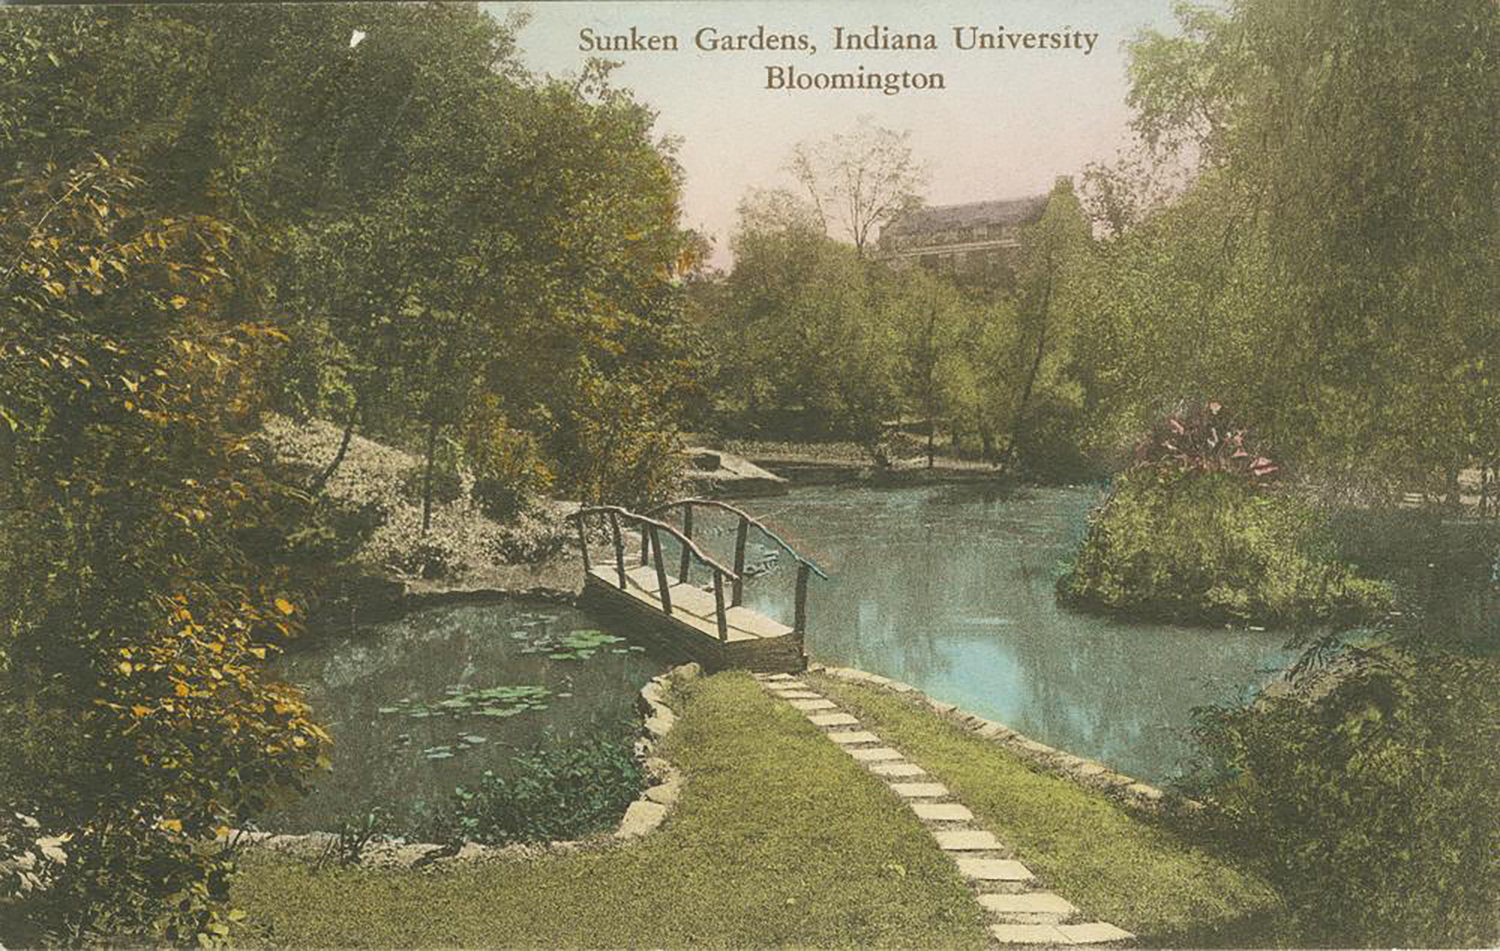
\includegraphics[keepaspectratio]{images/sunkgarden.jpg}}

}

\caption[Postcard of the Sunken Gardens]{Postcard of the Sunken Gardens.
The old Dunn Quarry on Third Street near Hawthorne Drive was converted
into a rock garden in 1928 to serve the recreational needs of the
campus. Known by students as the ``passion pit,'' it was demolished to
make way for the Jordan Hall greenhouse (now Biology Hall).
\textbf{Copyright holder unknown. Image from the
\href{https://libraries.indiana.edu/university-archives}{IU Archives}.}}

\end{figure}%

\bookmarksetup{startatroot}

\chapter*{Spring Break 2020: A New Watershed?}\label{sec-coda}
\addcontentsline{toc}{chapter}{Spring Break 2020: A New Watershed?}

\markboth{Spring Break 2020: A New Watershed?}{Spring Break 2020: A New
Watershed?}

\begin{figure}[H]

{\centering 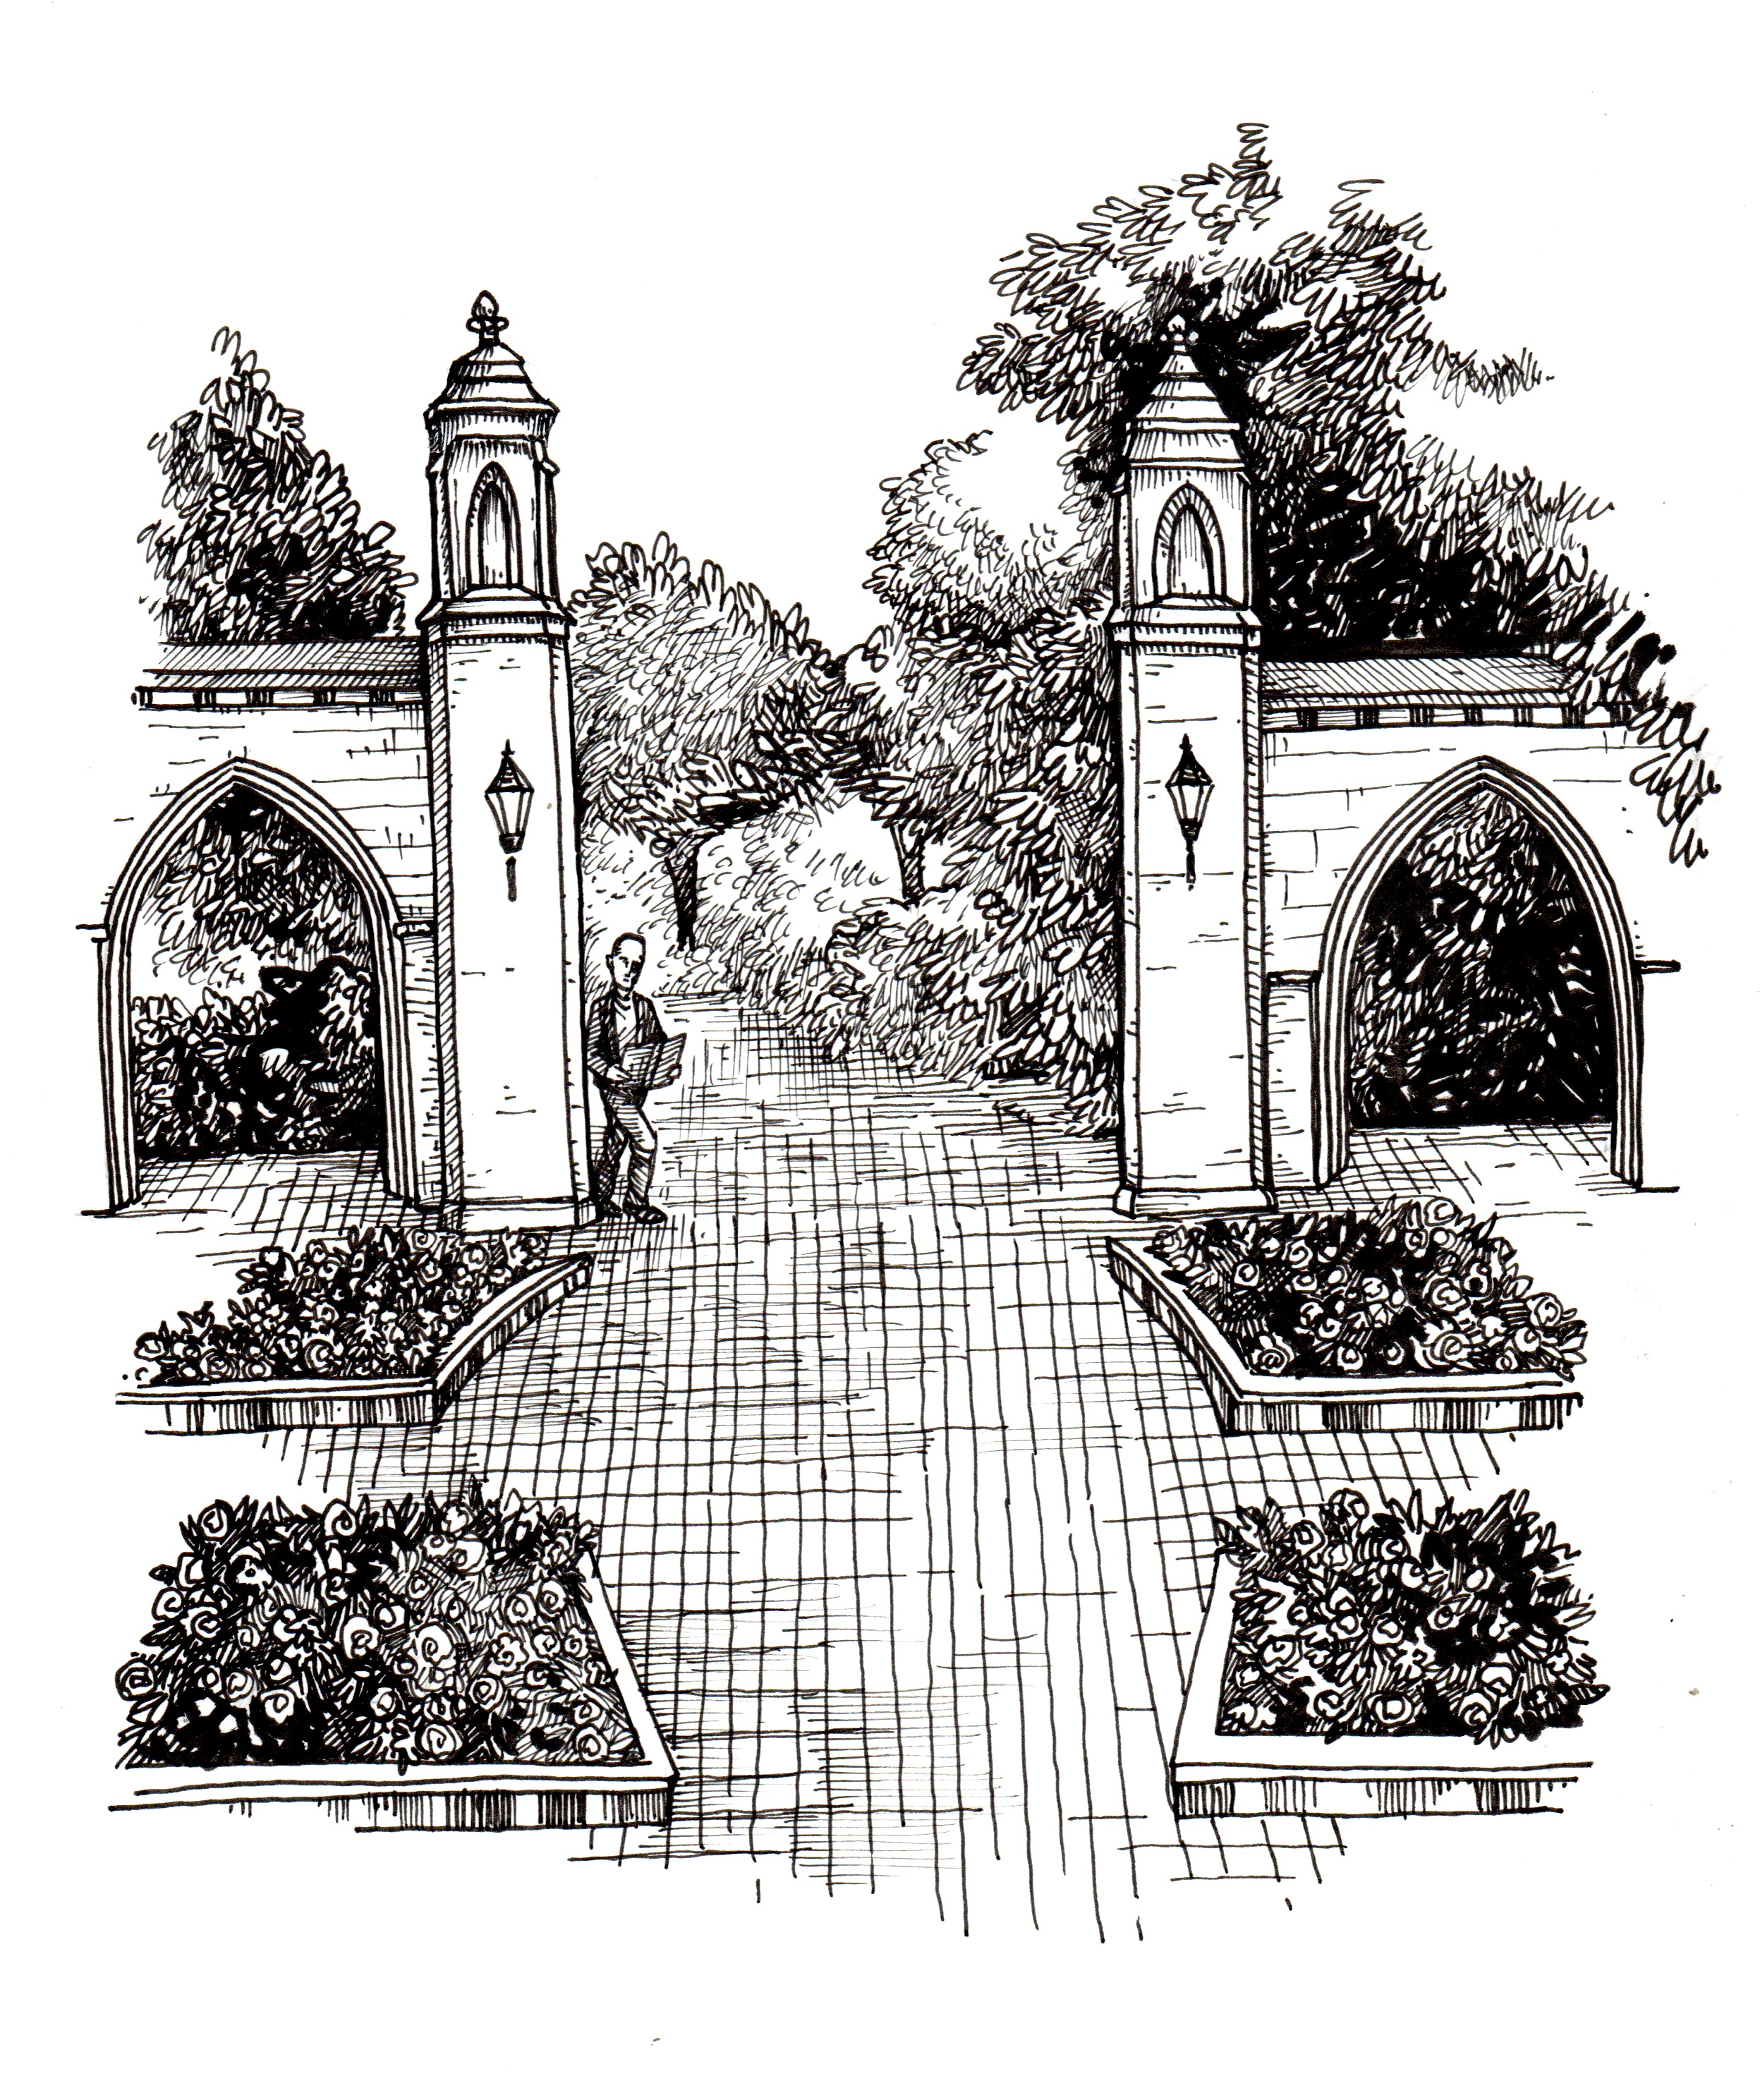
\includegraphics[width=0.6\linewidth,height=\textheight,keepaspectratio]{images/coda.jpeg}

}

\caption{Sample Gates}

\end{figure}%

\epigraph{
A watershed is a marvelous thing to consider: This process of rain falling, streams flowing, and oceans evaporating causes every molecule of water to make the complete trip once every two million years. The surface is carved into watersheds---kind of familial branching, a chart of relationship, and a definition of place. The watershed is the first and last nation, whose boundaries, though subtly shifting, are unarguable. Races of birds, subspecies of trees, and types of hats or rain gear go by the watershed. The watershed gives us a home, and a place to go upstream, downstream, or across in\ldots{}. Watershed consciousness\ldots{}is not just environmentalism\ldots{}but a move toward a profound citizenship in both the natural and the social worlds. If the ground can be our common ground, we can begin to talk to each other (human and non-human) once again.  
}
{---Gary Snyder, "Coming into the Watershed"}

Indiana University entered new institutional terrain in March 2020
around spring break with the arrival of a global pandemic. Tentative
plans to extend spring break another week were soon revised as the
magnitude of the public health crisis became apparent. As the Indiana
government issued directives for all state residents to shelter in
place, IU campuses around the state were closed and classes moved to
online learning delivered via the internet. Commencement ceremonies were
canceled, and the year-long commemoration of the IU bicentennial ceased
three months from its scheduled conclusion on June 30. At this writing,
four years later, the university has weathered this public health
crisis. A vaccination for COVID-19 was developed in record time,
in-person classes resumed, and social life returned, albeit to a new
normal.

What this means for American higher education more generally is still
too early to tell, but some think it represents a transition to a new
``watershed'' in our history. Literally, a watershed is a land area
where precipitation eventually flows into a body of water, usually a
river, lake, or ocean. So, the boundaries of a watershed are high points
on the land, like hilltops, ridges, or mountain crests. The Continental
Divide provided by the Rocky Mountains is an example of a large-scale
watershed boundary. Rainfall on the eastern side of the country flows
into the Atlantic Ocean; on the western side, the Pacific Ocean. On a
much smaller scale, the IU campus is bisected by a ridge, running near
Tenth Street, separating the land into two larger watersheds. On the
north side of campus, Griffy Creek and Cascades Creek drain into the
West Fork of the White River. On the south side, Clear Creek and Jackson
Creek drain into the East Fork of the White River. Both are the main
tributaries of the Wabash River. More than a third of the campus is
served by the Jordan River (renamed Campus River), which becomes part of
Clear Creek once it leaves campus.

Metaphorically, watersheds have rich connotations. Used to denote a
significant point of division or transition between two phases or
conditions, it can be applied to historical cases and used as a basis
for historical periodization. Dramatic change characterizes the movement
into a new watershed, as ``before'' and ``after'' acquire a new
relevance.

I suggest that Indiana University has operated in four historic
watersheds in the last two hundred years and is on the verge of a fifth.
The establishment of the institution in 1820 can be seen as the
watershed instauration, with a landscape of unique opportunities,
resources, and challenges. Located on Seminary Square, part of the
original congressional land grant that endowed the school, classes
started in 1825, and the college produced its first four graduates in
1830. The movement from seminary to college to university, the
curriculum based on classical languages, and the financial and political
challenges for the survival of a tiny institution were all part of the
institutional landscape of the early days. That first watershed ended
abruptly after a third of a century when the College Building burned
down in 1854.

That almost killed the university. But the town of Bloomington and the
small body of alumni rallied to provide financial and moral support, and
the institution rebuilt. Amid rebuilding, the institution's sole fiscal
allocation---the small University Fund endowment---was threatened by
legal maneuvering in 1855, but Governor Joseph A. Wright pressed the
legislature to restore the endowment, narrowly avoiding disaster for the
university. Wright happened to be among the students who attended when
the seminary first opened, although he never graduated.

Stronger due to overcoming critical challenges to its very existence, IU
went on for the next three decades, growing slowly in a time when higher
education had little relevance to the civic life of the state's
residents. The institutional landscape of this period saw the Civil War,
admission of women and African Americans as students, and the protracted
campaign to receive designation as a federal land-grant university under
the 1862 Morrill Act, which was unsuccessful. Instead, IU gained a
sibling state university---Purdue University in West Lafayette---as well
as a permanent rival.

This second watershed was upended by another campus fire, in 1883. The
newer of the two main buildings---Science Hall---was destroyed. Unlike
in 1854, it did not threaten the university's continued existence,
although it was a hard blow. By that time, the university had acquired
enough institutional momentum to carry it through. It prompted the board
of trustees to make a fateful decision to move the campus across town,
to a patch of farm woodlot known as Dunn's Woods. In 1885, the campus
acquired a new leader, President David Starr Jordan, a research
scientist with a national reputation. Focused on investigation as the
basis for teaching as well as research, his administration modernized
the curriculum, instituted the elective system, and reorganized the
faculty into departments. The university's aspirations were elevated as
it became involved in national dialogues about higher education,
research, and the role of universities in America.

For over a half century, IU operated in this environment. It grew
steadily, through the turn of the twentieth century, the First World
War, and the Great Depression of the 1930s, much of it under the
leadership of William Lowe Bryan, another research scientist and the
protégé of Jordan. It was not until the advent of the Second World War
and its aftermath that IU entered another watershed.

Starting in 1945, the postwar landscape for American higher education
was changed significantly as the federal government subsidized college
education for military veterans through the GI Bill and invested heavily
in research and development as an important basis for national security.
This ``golden age'' of rising enrollments and ample funding lasted until
the early 1970s when the political and social environment changed. In
the next two decades, American higher education reached the status of a
``mature industry,'' as one observer noted, as competition for students,
funding, and reputation became even more pronounced.\footnote{\citeproc{ref-levine1997a}{Arthur
  Levine, {``How the Academic Profession Is Changing,''} \emph{Daedalus}
  126, no. 4 (1997): 1--20}; \citeproc{ref-levine1997b}{{``Higher
  Education Becomes a Mature Industry,''} \emph{About Campus: Enriching
  the Student Learning Experience} 2, no. 3 (1997): 31--32,
  \url{https://doi.org/10.1177/108648229700200}}.}

In the early years of the twenty-first century, the major features of
the post--World War II watershed were still in place, although buffeted
by ceaseless political winds as American society and culture underwent
change. While still serving the education and knowledge needs of the
state of Indiana, this long-lasting institutional watershed was becoming
increasingly globalized, and student tuition and private philanthropy
assumed greater importance in the university's budget as state
legislative support slowly dwindled.

Looking back over the two-hundred-plus-year history of Indiana
University from the present, one can generalize some broad themes. IU
has grown into a multifaceted educational enterprise with a myriad of
connections to local communities, the Hoosier state, the nation, and the
world. Its education, research, and service missions grew out of the
flagship campus in Bloomington during its first century. In the second
century, the university extended its programs statewide and developed
physical campuses in several Hoosier communities. As a human
institution, IU remains in constant flux, responding internally to
cultural imperatives of teaching and learning as well as reacting to the
myriad external demands placed on it.

In keeping with the focus of this book on how the university was shaped
by its history and physical environment, watershed periods provide a way
to examine large-scale changes. There is no question that 2020 will go
down in IU's history as a significant year, perhaps marking a new
watershed. But the meaning of that year to the history of Indiana
University is still being written.

\bookmarksetup{startatroot}

\chapter*{Campus Expansion Map
(1885--2020)}\label{campus-expansion-map-18852020}
\addcontentsline{toc}{chapter}{Campus Expansion Map (1885--2020)}

\markboth{Campus Expansion Map (1885--2020)}{Campus Expansion Map
(1885--2020)}

\begin{figure}[H]

{\centering 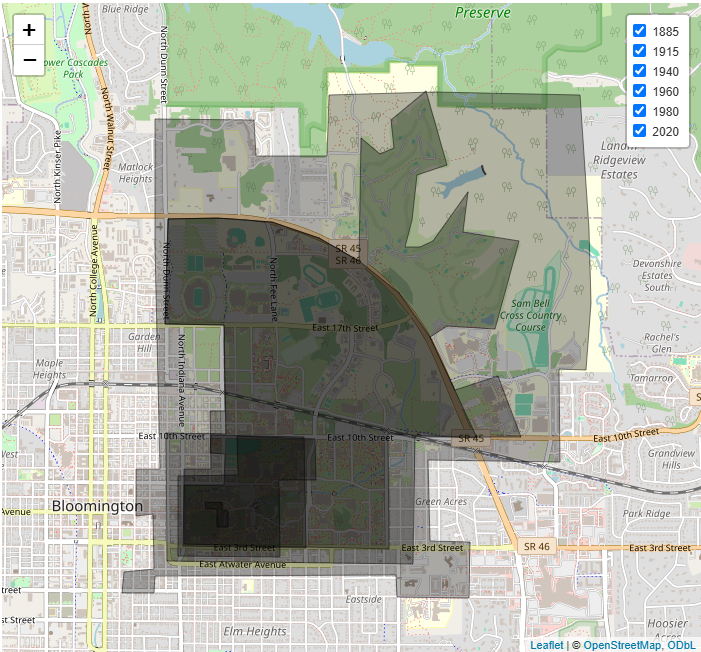
\includegraphics[width=0.85\linewidth,height=\textheight,keepaspectratio]{images/imap.PNG}

}

\caption[Static version of the IU campus footprint map
(1885--2020)]{Static version of the IU campus footprint map
(1885--2020), based on official campus maps, from twenty acres at the
beginning to nearly 2,000 acres at present. The interactive version is
available in the HTML edition.}

\end{figure}%

\bookmarksetup{startatroot}

\chapter*{Acknowledgments}\label{acknowledgments}
\addcontentsline{toc}{chapter}{Acknowledgments}

\markboth{Acknowledgments}{Acknowledgments}

\begin{figure}[H]

{\centering 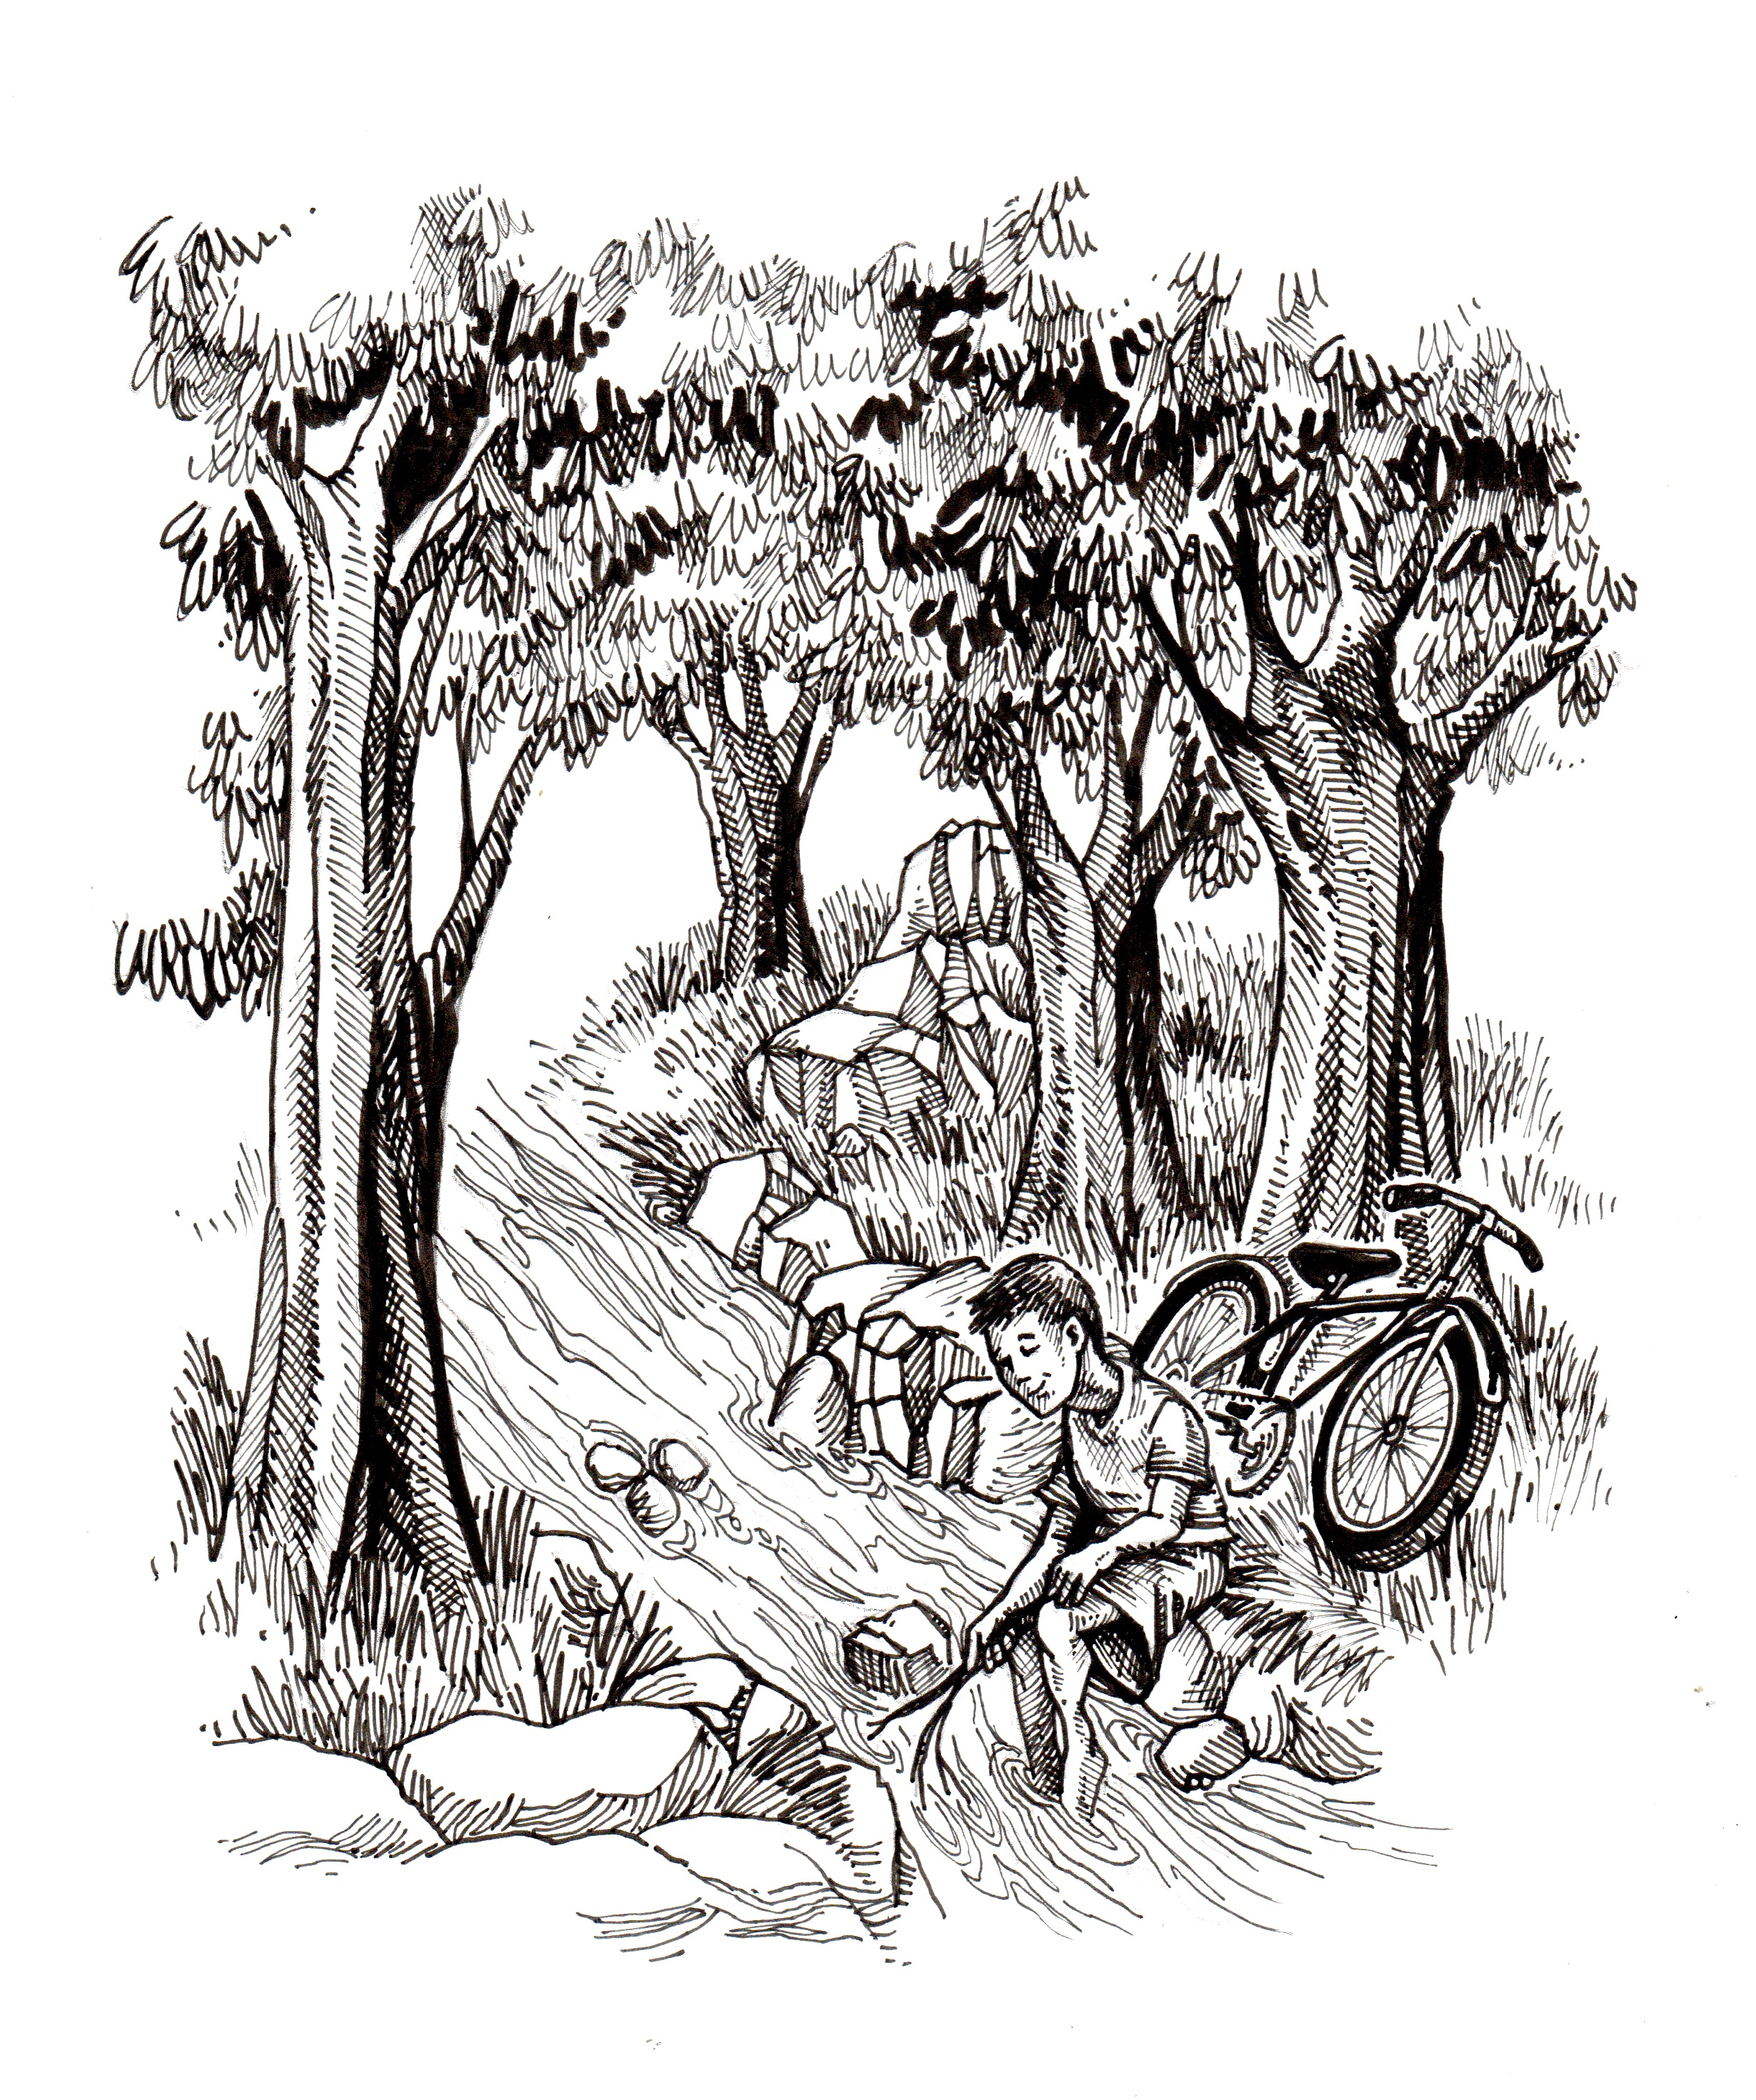
\includegraphics[width=0.6\linewidth,height=\textheight,keepaspectratio]{images/acknowledgements.jpeg}

}

\caption{Boy with bicycle at Jordan River}

\end{figure}%

\begin{anecdote}
A scrawny boy, aged nine, pedaled his twenty-inch red Schwinn bicycle up Woodlawn Avenue from Bryan Park to the Indiana University campus, looking for adventure. The warm spring air was full of mysterious promise. Accompanied by a friend who lived across the street on Maxwell Lane and one of his brothers, the boys knew that winding paths through the woods, immense gray buildings, and running water would await them. Once on campus grounds, anticipation gave way to delight in the present moment---riding endlessly on interconnected walkways, catching goldfish in the creek left discarded from fraternity parties, searching for a drinking fountain in the cavernous Union building. The waking reverie lasted until the lengthening shadows brought them back to the hunger in their bellies and to the relief of their homes. In the spring and summer of 1964, that boy was introduced to the wonders of university life by the physical environment of the campus, where he was able to engage all of his senses, six blocks away from his home. Still innocent of the ways of place-making, the names Maxwell and Bryan held no connotations. The boy's name was Jimmy Capshew, and he has lived in the university's sheltering shadow since.
\end{anecdote}

This book was a long time in the making, delayed by the global pandemic.
Along the way, I received assistance from many people, most notably from
the excellent staff of the University Archives at Indiana University
Bloomington. I am grateful to my colleagues Dina Kellams, Kristin
Leaman, Carrie Schwier, Mary Mellon, Molly Wittenberg, Brad Cook, and
Amanda Rindler.

In 2015, I was drawn into the organization and then operation of the IU
Office of the Bicentennial under its mastermind, Kelly Kish, whose
administrative acumen is matched only by her prodigious intellect. She
always asked the hard questions, but I could count on her for unflagging
support. The staff of the Bicentennial Office, including Bre Anne Kusz,
Jeremy Hackerd, Sarah Jacobi, Angel Nathan, Sarah Reynolds, Rafal
Swiatkowski, and Brittany Terwilliger, buoyed my efforts at every turn.

I made presentations to several audiences, both local and national,
about the research on which this book is based, including the Monroe
County History Club, the IU Alumni Association's Mini University, the
Friends of the Monroe County Public Library, and the History of
Education Society.

Several persons facilitated access to documents and shared relevant
information, including Anita Bracalente, Jonah Busch, Greg Buse, Carey
Champion, Terry Clapacs, Michael Chitwood, Bridget Edwards, Harry Ford,
Deborah Lemon, Richard McClelland, Sarah Mincey, David Parkhurst, Eileen
Savage, and Indermohan Virk.

The people who read drafts of chapters occupy a high niche in my
personal pantheon: Bre Anne Kusz, Jonah Busch, Duncan Campbell, Carey
Champion, Michael Chitwood, Harry Ford, Donald J. Gray, Jeremy Hackerd,
Sarah Mincey, Michael Nelson, Laura Plummer, Sarah Reynolds, Eric
Sandweiss, Curt Simic, and John Summerlot. It was a pleasure working
with illustrator Joe Lee, whom I first met two decades ago.

When the time came to publish this research, Diane Dallis-Comentale,
Ruth Lilly Dean of University Libraries, suggested I try the new
publishing service provided by the Department of Scholarly
Communication. Adam Mazel, Digital Publishing Librarian, was an
excellent guide and an effective colleague in creating my first ``born
digital'' book. The interactive map was made possible through the
innovative efforts of Theresa Quill, Map and Spatial Data librarian.

A special thanks goes to Michael McRobbie, University Chancellor and
President Emeritus, who had faith in planning for the university's
future by a thorough understanding of its past.

\begin{flushright}
Halloween 2024
\end{flushright}

\bookmarksetup{startatroot}

\chapter*{Bibliography}\label{bibliography}
\addcontentsline{toc}{chapter}{Bibliography}

\markboth{Bibliography}{Bibliography}

\phantomsection\label{refs}
\begin{CSLReferences}{1}{0}
\bibitem[\citeproctext]{ref-ids1898a}
\emph{Indiana Student}, April 1, 1898, 53.

\bibitem[\citeproctext]{ref-is1901a}
\emph{Indiana Student}, April 6, 1901, 12.

\bibitem[\citeproctext]{ref-arbutus1906a}
\emph{Arbutus}, June 1906, 388--90.

\bibitem[\citeproctext]{ref-ids1999a}
\emph{Indiana Daily Student}, November 15, 1999.

\bibitem[\citeproctext]{ref-bt1884a}
\emph{Bloomington Telephone} 7, no. 46 (March 29, 1884): 1.

\bibitem[\citeproctext]{ref-iua_c213_b30}
Bloomington: Indiana University Archives, n.d. IUA/C213/B30/F.

\bibitem[\citeproctext]{ref-iuChamness}
{``{About Ivy L. Chamness},''} n.d.
\url{https://honorsandawards.iu.edu/awards/honoree/2297.html}.

\bibitem[\citeproctext]{ref-abram1996a}
Abram, David. \emph{The Spell of the Sensuous: Perception and Language
in a More-Than-Human World}. New York: Vintage, 1996.

\bibitem[\citeproctext]{ref-adair1974a}
Adair, Douglass. \emph{Fame and the Founding Fathers: Essays by Douglass
Adair}. Edited by Trevor Colburn. New York: W. W. Norton \& Company,
1974.

\bibitem[\citeproctext]{ref-addis1839a}
Addis, Alfred. {``Latin Grammars.''} \emph{The Literary and Theological
Review} 6, no. 21 (1839): 59--66.

\bibitem[\citeproctext]{ref-albert1982a}
Albert, Barb. {``{I.U.} Group Launches Battle to Rescue Beloved
Woods.''} \emph{Indianapolis Star}, February 12, 1982, 22.

\bibitem[\citeproctext]{ref-iuaq1919a}
{``Alumni Council Meetings.''} \emph{Indiana University Alumni
Quarterly} 6, no. 3 (July 1919): 392--94.

\bibitem[\citeproctext]{ref-iuaq1937b}
{``Alumni Notes by Classes: 1906.''} \emph{Indiana University Alumni
Quarterly} 24, no. 1 (1937): 74.

\bibitem[\citeproctext]{ref-arbutus1899a}
{``Balls and Strikes: A Story.''} \emph{Arbutus}, 1899, 174--79.

\bibitem[\citeproctext]{ref-banta1881a}
Banta, D. D. \emph{A Historical Sketch of Johnson County, Indiana}.
Chicago: J.H. Beers \& Co., 1881.

\bibitem[\citeproctext]{ref-banta1914b}
Banta, David D. {``History of Indiana University {I}: The Seminary
Period (1820--1828).''} \emph{Indiana University Alumni Quarterly} 1,
no. 1 (1914): 3--24.

\bibitem[\citeproctext]{ref-banta1914c}
Banta, David D. {``History of Indiana University: II: From Seminary to
College (1826--1829).''} \emph{Indiana University Alumni Quarterly} 1,
no. 2 (1914): 142--65.

\bibitem[\citeproctext]{ref-banta1914d}
Banta, David D. {``History of Indiana University: III: The New Departure
(1829--1833).''} \emph{Indiana University Alumni Quarterly} 1, no. 3
(1914): 272--92.

\bibitem[\citeproctext]{ref-banta1914a}
Banta, David D. {``History of Indiana University: IV. The {`Faculty
War'} of 1832.''} \emph{Indiana University Alumni Quarterly} 1, no. 4
(1914): 369--86.

\bibitem[\citeproctext]{ref-banta1915a}
Banta, David D. {``History of Indiana University: V: From College to
University (1833--1838).''} \emph{Indiana University Alumni Quarterly}
2, no. 1 (1915): 5--17.

\bibitem[\citeproctext]{ref-banta1915b}
Banta, David D. {``History of Indiana University: VI: Perils from
Sectarian Controversies and the Constitutional Convention
(1838--1850).''} \emph{Indiana University Alumni Quarterly} 2, no. 2
(1915): 99--110.

\bibitem[\citeproctext]{ref-banta1889a}
Banta, David D. {``Letter to James Woodburn.''} Indiana University
Archives, February 9, 1889.

\bibitem[\citeproctext]{ref-banta1883a}
Banta, David D. \emph{Indiana Student} 9, no. 7 (May 1883): 166--67.

\bibitem[\citeproctext]{ref-benson1884a}
Benson, Olof. {``Description of the Plan of Improvement of University
Park.''} Indiana University Archives/C77/B1, 1884.

\bibitem[\citeproctext]{ref-bernstein1982a}
Bernstein, Leonard. {``Letter to David {F.} Parkhurst,''} February 13,
1982. David F. Parkhurst files.

\bibitem[\citeproctext]{ref-bischoff1970a}
Bischoff, Sue. {``Nelson Pleased by Turnout, Originality.''}
\emph{Indiana Daily Student}, n.d.

\bibitem[\citeproctext]{ref-blanchard1884a}
Blanchard, Charles, ed. \emph{Counties of Morgan, Monroe, and Brown,
Indiana: Historical and Biographical}. Chicago: F.A. Battey \& Co.,
1884.

\bibitem[\citeproctext]{ref-blanck1959a}
Blanck, Jacob. \emph{Bibliography of American Literature}. Vol. 3. New
Haven: Yale University Press, 1959.

\bibitem[\citeproctext]{ref-bracalente2012a}
Bracalente, Anita. {``Indiana University's Woodland Campus.''}
\emph{View} 12 (2012): 25--27.

\bibitem[\citeproctext]{ref-brichford1971a}
Brichford, Maynard. \emph{Journal of the Illinois State Historical
Society (1908--1984)} 64, no. 3 (1971): 355--56.
\url{http://www.jstor.org/stable/40190803}.

\bibitem[\citeproctext]{ref-brichford1975a}
Brichford, Maynard. \emph{Journal of the Illinois State Historical
Society (1908--1984)} 68, no. 3 (1975): 297--99.
\url{http://www.jstor.org/stable/40191173}.

\bibitem[\citeproctext]{ref-brogan1982a}
Brogan, Dan. {``Plager's Contempt on Compromise Out of Character for Law
Profession.''} \emph{Indiana Daily Student}, February 19, 1982.

\bibitem[\citeproctext]{ref-brown2012a}
Brown, William M., and Michael W. Hamburger. {``Organizing for
Sustainability.''} In \emph{Enhancing Sustainability Campuswide}, edited
by Bruce A. Jacobs and Jillian Kinzie, 83--96. New Directions for
Student Services 137. Wiley, 2012.

\bibitem[\citeproctext]{ref-bryan1916a}
Bryan, William. {``Letter to George Kessler.''} Indiana University
Archives C286/B150/F Kessler, George, May 25, 1916.

\bibitem[\citeproctext]{ref-bryan1929a}
Bryan, William Lowe. {``Letter to James {A.} Woodburn.''} Indiana
University Archives, June 17, 1929. IUA/C83/B3/F Publications, Galleys,
\& Transcripts.

\bibitem[\citeproctext]{ref-bryan1934a}
Bryan, William Lowe. {``Letter to James {A.} Woodburn.''} Indiana
University Archives, November 17, 1934. IUA/C83/B3/F Publications,
Galleys, \& Transcripts.

\bibitem[\citeproctext]{ref-buley1950a}
Buley, R. Carlyle. \emph{The Old Northwest: Pioneer Period, 1815--1840}.
Vol. 2. Bloomington: Indiana University Press, 1950.

\bibitem[\citeproctext]{ref-bunnage1999a}
Bunnage, JoAnn C. {``Barbara Shalucha and the Development of Hilltop
Garden and Nature Center: The Cultivation of a Community Treasure,''}
1999.

\bibitem[\citeproctext]{ref-burgess2011a}
Burgess, Jo, ed. \emph{Affectionately Yours: The Andrew Wylie Family
Letters}. I: 1828--1859, II: 1860--1918 vols. Bloomington: Wylie House
Museum, 2011. Volume I:
\url{https://scholarworks.iu.edu/dspace/items/4323e65e-8053-4624-a19c-cec3c14205f0};
Volume II:
\url{https://scholarworks.iu.edu/dspace/items/4c56273e-06d6-427e-a533-769e9cf5504e}.

\bibitem[\citeproctext]{ref-busch2000a}
Busch, Jonah M. {``The Protect Griffy Alliance and the Golf War:
Collective Action at Its Finest,''} April 28, 2000. seminar paper,
Indiana University.

\bibitem[\citeproctext]{ref-caldwell1963a}
Caldwell, Lynton K. {``Environment: A New Focus for Public Policy?''}
\emph{Public Administration Review} 23 (1963): 132--39.

\bibitem[\citeproctext]{ref-caldwell1997a}
Caldwell, Lynton Keith. {``Foreword: A Sense of Place.''} In \emph{The
Natural Heritage of Indiana}, edited by Marion C. Jackson, xv--xvi.
Bloomington: Indiana University Press, 1997.

\bibitem[\citeproctext]{ref-campbell1882a}
Campbell, Matthew. {``Letter to David Banta.''} Indiana University
Archives/C112/B1, December 25, 1882.

\bibitem[\citeproctext]{ref-ids1904a}
{``Campus Improvements Due to Prof. Mottier.''} \emph{Indiana Daily
Student}, February 5, 1904, 1.

\bibitem[\citeproctext]{ref-capshew2012a}
Capshew, James H. \emph{Herman {B} Wells: The Promise of the American
University}. Bloomington; Indianapolis: Indiana University Press;
Indiana Historical Society Press, 2012.

\bibitem[\citeproctext]{ref-capshew2011a}
Capshew, James H. {``Indiana University as the {`Mother of College
Presidents'}: Herman {B} Wells as Inheritor, Exemplar, and Agent.''}
Bloomington: IU Institute for Advanced Study, 2011.
\url{https://hdl.handle.net/2022/14123}.

\bibitem[\citeproctext]{ref-capshew1999a}
Capshew, James H. {``IU Country Club?''} \emph{Herald-Times}, September
4, 1999.

\bibitem[\citeproctext]{ref-capshew2019a}
Capshew, James H. {``Memo University Seal.''} Reference file: University
Seal. Indiana University Archives, March 1, 2019.

\bibitem[\citeproctext]{ref-capshew2018a}
Capshew, James H. {``New Light on an Old Story: The Secret of the
Faculty War.''} \emph{200: The Bicentennial Magazine} 1, no. 1 (2018):
6--8.

\bibitem[\citeproctext]{ref-capshew1999b}
Capshew, James H. {``Nicklaus Course Raises Questions.''}
\emph{Herald-Times}, no. editorial (September 8, 1999).

\bibitem[\citeproctext]{ref-capshew2009a}
Capshew, James H. {``The Campus as a Pedagogical Agent: Herman Wells,
Cultural Entrepreneurship, and the Benton Murals.''} \emph{Indiana
Magazine of History} 105, no. 2 (2009): 179--97.
\url{https://www.jstor.org/stable/27792978}.

\bibitem[\citeproctext]{ref-carleton1902a}
Carleton, Emma. {``About the New Purchase.''} \emph{Indianapolis News},
May 16, 1902.

\bibitem[\citeproctext]{ref-carmichael1969a}
Carmichael, Hoagy. \emph{The Stardust Road}. 1946. Reprint, New York:
Greenwood Press, 1969.

\bibitem[\citeproctext]{ref-carmichael1965a}
Carmichael, Hoagy, and Stephen Longstreet. \emph{Sometimes i Wonder: The
Story of Hoagy Carmichael}. New York: Farrer, Straus; Giroux, 1965.

\bibitem[\citeproctext]{ref-carr1961a}
Carr, Edward Hallett. \emph{What Is History?} New York: Knopf, 1961.

\bibitem[\citeproctext]{ref-cassidy1985a}
Cassidy, Frederic G., ed. \emph{Dictionary of American Regional
English}. Cambridge, MA: Belknap Press of Harvard University Press,
1985.

\bibitem[\citeproctext]{ref-cep2011a}
Center on Education Policy. {``Public Schools and the Original Federal
Land Grant Program: A Background Paper from the Center on Education
Policy.''} Washington, 2011-04. \url{https://eric.ed.gov/?id=ED518388}.

\bibitem[\citeproctext]{ref-chamness1919a}
Chamness, Ivy. {``Letter to Alumni Council.''} Indiana University
Archives, March 22, 1919. IUA/C286/B54.

\bibitem[\citeproctext]{ref-chamness1938b}
Chamness, Ivy. {``Letter to Herman {B} Wells.''} Indiana University
Archives, 1938. IUA/C213/B118.

\bibitem[\citeproctext]{ref-chamness1940a}
Chamness, Ivy. {``Letter to James {A.} Woodburn.''} Indiana University
Archives, November 30, 1940. IUA/C83/B4/F Testimonial
Banquet/Correspondence.

\bibitem[\citeproctext]{ref-chamness1935a}
Chamness, Ivy. {``Letter to Mrs. C. J. Sembower.''} Indiana University
Archives, June 3, 1935. IUA/C84/B1/F Edited Manuscripts-Alumni
Quarterly.

\bibitem[\citeproctext]{ref-chamness1919b}
Chamness, Ivy. {``Letter to William Lowe Bryan.''} Indiana University
Archives, June 18, 1919. IUA/C286/B54.

\bibitem[\citeproctext]{ref-chamness1920a}
Chamness, Ivy. {``Letter to William Lowe Bryan.''} Indiana University
Archives, May 11, 1920. IUA/C286/B54.

\bibitem[\citeproctext]{ref-chamness1923b}
Chamness, Ivy L. {``Another College President.''} \emph{IU Alumni
Quarterly} 10 (1923): 512.

\bibitem[\citeproctext]{ref-chamness1938a}
Chamness, Ivy L. {``Another College President.''} \emph{IU Alumni
Quarterly} 25 (1938): 59.

\bibitem[\citeproctext]{ref-chamness1921a}
Chamness, Ivy L., ed. \emph{Indiana University, 1820--1920: Centennial
Memorial Volume}. Bloomington: Indiana University, 1921.

\bibitem[\citeproctext]{ref-chamness1929a}
Chamness, Ivy L. {``Indiana University in Earlier Days: I. As Reflected
in Commencement and Exhibition Programs.''} \emph{Indiana University
Alumni Quarterly} 16, no. 1 (1929): 33--45.

\bibitem[\citeproctext]{ref-chamness1929b}
Chamness, Ivy L. {``Indiana University in Earlier Days: II. As Reflected
in Early Issues of the \emph{Indiana Student}.''} \emph{Indiana
University Alumni Quarterly} 16, no. 2 (1929): 199--221.

\bibitem[\citeproctext]{ref-chamness1921b}
Chamness, Ivy L. {``Indiana University---Mother of College
Presidents.''} \emph{Educational Issues} 2, no. 8 (1921): 28--29.

\bibitem[\citeproctext]{ref-chamness1922a}
Chamness, Ivy L. {``Indiana University---Mother of College
Presidents.''} \emph{Indiana University Alumni Quarterly} 9 (1922):
46--49.

\bibitem[\citeproctext]{ref-chamness1000a}
Chamness, Ivy L. {``IUA/C84/B1/f Edited Manuscripts-Myers.''}
Bloomington, IN: Indiana University Archives, n.d.

\bibitem[\citeproctext]{ref-chamness1923a}
Chamness, Ivy L. {``More College Presidents.''} \emph{IU Alumni
Quarterly} 10 (1923): 334.

\bibitem[\citeproctext]{ref-chamness1945a}
Chamness, Ivy L. {``The First 125 Years.''} \emph{Indiana Alumni
Magazine} 7, no. 9 (1945): 11--14.

\bibitem[\citeproctext]{ref-chamness1928a}
Chamness, Ivy Leone. {``A Study of Editorial Matters in the Catalogs of
the Members of the National Association of State Universities.''}
Indiana University, 1928. Master's thesis, Indiana University.

\bibitem[\citeproctext]{ref-chamness1915b}
Chamness, Ivy Leone. {``Alumni Notes by Classes.''} Edited by Ivy Leone
Chamness. \emph{Indiana University Alumni Quarterly} 2, no. 2 (April
1915): 207.

\bibitem[\citeproctext]{ref-chamness1930a}
Chamness, Ivy Leone. {``Indiana University in Earlier Days: III. As
Reflected in the Issues of the \emph{Indiana Student} in the
Nineties.''} \emph{Indiana University Alumni Quarterly} 17, no. 1
(1930): 22--38.

\bibitem[\citeproctext]{ref-chamness1931a}
Chamness, Ivy Leone. {``Indiana University in Earlier Days: IV. As
Reflected in Issues of the \emph{Indiana Student} in the Nineties.''}
\emph{Indiana University Alumni Quarterly} 18, no. 2 (1931): 156--71.

\bibitem[\citeproctext]{ref-chamness1931b}
Chamness, Ivy Leone. {``Indiana University in Earlier Days: V. As
Reflected in Historical Material Recently Given to the Institution.''}
\emph{Indiana University Alumni Quarterly} 18, no. 1 (1931): 16--29.

\bibitem[\citeproctext]{ref-chamness1933a}
Chamness, Ivy Leone. {``Indiana University in Earlier Days: VI. As
Reflected in Official Publications.''} \emph{Indiana University Alumni
Quarterly} 20, no. 2 (1933): 159--68.

\bibitem[\citeproctext]{ref-chamness1934a}
Chamness, Ivy Leone. {``Indiana University in Earlier Days: VII. As
Reflected in Official Publications.''} \emph{Indiana University Alumni
Quarterly} 21, no. 2 (1934): 34--47.

\bibitem[\citeproctext]{ref-chapman2006a}
Chapman, M. Perry. \emph{American Places: In Search of the Twenty-First
Century Campus}. Westport, CT: Praeger, 2006.

\bibitem[\citeproctext]{ref-iuaq1937a}
{``{Charles H. Hays}.''} \emph{Indiana University Alumni Quarterly} 24
(1937): 511--12.

\bibitem[\citeproctext]{ref-iam1957a}
{``{Charles H. Hays}.''} \emph{Indiana Alumni Magazine} 19, no. 7
(1957): 1.

\bibitem[\citeproctext]{ref-chaudemanche2000a}
Chaudemanche, Diane, and Elaine Herold, eds. \emph{Andrew Wylie: A
Bibliography}, 2000. \url{http://hdl.handle.net/2022/20329}.

\bibitem[\citeproctext]{ref-clapacs2017a}
Clapacs, J. Terry. \emph{Indiana University Bloomington: America's
Legacy Campus}. Bloomington: Indiana University Press, 2017.

\bibitem[\citeproctext]{ref-clark1970a}
Clark, Thomas D. \emph{Indiana University: Midwestern Pioneer}. 4 vols.
Bloomington: Indiana University Press, 1970/1977.

\bibitem[\citeproctext]{ref-clark1970b}
Clark, Thomas D. \emph{Indiana University: Midwestern Pioneer: Volume
{I}: The Early Years}. 4 vols. Bloomington: Indiana University Press,
1970.

\bibitem[\citeproctext]{ref-clark1973a}
Clark, Thomas D. \emph{Indiana University: Midwestern Pioneer: Volume
{II}: In Mid-Passage}. 4 vols. Bloomington: Indiana University Press,
1973.

\bibitem[\citeproctext]{ref-clark1977a}
Clark, Thomas D. \emph{Indiana University: Midwestern Pioneer: Volume
{III}: Years of Fulfillment}. 4 vols. Bloomington: Indiana University
Press, 1977.

\bibitem[\citeproctext]{ref-cokinos1982e}
Cokinos, Christopher. {``Bernstein Note Indicates Support for {`Save the
Woods'}.''} \emph{Indiana Daily Student}, February 19, 1982.

\bibitem[\citeproctext]{ref-cokinos1982a}
Cokinos, Christopher. {``Law Addition Sparks Dispute over Woods.''}
\emph{Indiana Daily Student}, January 19, 1982.

\bibitem[\citeproctext]{ref-cokinos1982d}
Cokinos, Christopher. {``Law School Addition Plans to Be Resubmitted.''}
\emph{Indiana Daily Student}, 1982-02-11.

\bibitem[\citeproctext]{ref-cokinos1982j}
Cokinos, Christopher. {``Law School Expansion Inquiry Buried.''}
\emph{Indiana Daily Student}, March 31, 1982.

\bibitem[\citeproctext]{ref-cokinos1982b}
Cokinos, Christopher. {``Law School Expansion May Incapacitate
Observatory.''} \emph{Indiana Daily Student}, January 21, 1982, 1.

\bibitem[\citeproctext]{ref-cokinos1982i}
Cokinos, Christopher. {``New Addition Plan Would Save Woods.''}
\emph{Indiana Daily Student}, April 2, 1982.

\bibitem[\citeproctext]{ref-cokinos1982f}
Cokinos, Christopher. {``Ryan Requests Look at Options for Law
School.''} \emph{Indiana Daily Student}, February 25, 1982.

\bibitem[\citeproctext]{ref-cokinos1982c}
Cokinos, Christopher. {``Save the Woods Group Organizing to Protect Old
Crescent.''} \emph{Indiana Daily Student}, February 10, 1982, 3.

\bibitem[\citeproctext]{ref-cokinos1982h}
Cokinos, Christopher. {``State to Determine If Law Applies to IU
Expansion.''} \emph{Indiana Daily Student}, March 12, 1982.

\bibitem[\citeproctext]{ref-cokinos1982k}
Cokinos, Christopher. {``Wells: University to Develop Campus
Natural-Areas Policy.''} \emph{Indiana Daily Student}, April 30, 1982,
2.

\bibitem[\citeproctext]{ref-cokinos1982g}
Cokinos, Christopher, and Barbara Toman. {``Trustees to Hear Law
Expansion Opposition.''} \emph{Indiana Daily Student}, March 5, 1982.

\bibitem[\citeproctext]{ref-collins1992a}
Collins, Dottie. {``Conversations about the Bloomington Campus: It Isn't
Easy Being Green (but Planning Ahead Helps).''} \emph{The College} 16,
no. 2 (1992): 8--11.

\bibitem[\citeproctext]{ref-iuaq1938a}
{``Commencement, 1938.''} \emph{Indiana University Alumni Quarterly} 25,
no. 3 (1938): 298--337.

\bibitem[\citeproctext]{ref-conway2004a}
Conway, Thomas G. {``Finding America's History.''} \emph{Journal of the
Illinois State Historical Society} 97, no. 2 (2004): 92--106.

\bibitem[\citeproctext]{ref-ces1999a}
Council for Environmental Stewardship. {``Annual Report,''} 1998--1999.

\bibitem[\citeproctext]{ref-ces2002a}
Council for Environmental Stewardship. {``Annual Report,''} 2001--2002.

\bibitem[\citeproctext]{ref-ces2003a}
Council for Environmental Stewardship. {``Annual Report,''} 2002--2003.

\bibitem[\citeproctext]{ref-counts2002a}
Counts, Will, James H. Madison, and Scott Russell Sanders.
\emph{Bloomington Past and Present}. Bloomington: Indiana University
Press, 2002.

\bibitem[\citeproctext]{ref-cravens1915a}
Cravens, J. W. {``History of University Land Purchases.''} \emph{Indiana
University Alumni Quarterly} 2, no. 2 (1915): 156--59.

\bibitem[\citeproctext]{ref-cravens1922b}
Cravens, John W. {``Buildings on the Old and New Campuses of Indiana
University: I. The Old Seminary Building.''} \emph{Indiana University
Alumni Quarterly} 9, no. 1 (1922): 1--11.

\bibitem[\citeproctext]{ref-cravens1922a}
Cravens, John W. {``Buildings on the Old and New Campuses of Indiana
University: II: Six of the Buildings on the Old Campus.''} \emph{Indiana
University Alumni Quarterly} 9, no. 2 (1922): 156--64.

\bibitem[\citeproctext]{ref-cravens1922c}
Cravens, John W. {``Buildings on the Old and New Campuses of Indiana
University: III. Buildings on the New Campus and Elsewhere in Monroe
County.''} \emph{Indiana University Alumni Quarterly} 9, no. 3 (1922):
303--20.

\bibitem[\citeproctext]{ref-cravens1927a}
Cravens, John W. {``The Trustees of Indiana University.''} \emph{Indiana
University Alumni Quarterly} 14 (1927): 465--83.

\bibitem[\citeproctext]{ref-cumings1911a}
Cumings, E. R. {``The Geological Conditions of Municipal Water Supply in
the Driftless Area of Southern Indiana.''} \emph{Proceedings of the
Indiana Academy of Science} 21 (1911): 111--46.
\url{https://journals.indianapolis.iu.edu/index.php/ias/article/view/14025}.

\bibitem[\citeproctext]{ref-curti1975a}
Curti, Merle. \emph{The American Historical Review} 80, no. 3 (1975):
518--19. \url{https://doi.org/10.2307/1850710}.

\bibitem[\citeproctext]{ref-curti1978a}
Curti, Merle. \emph{The American Historical Review} 83, no. 4 (1978):
1101. \url{https://doi.org/10.2307/1867836}.

\bibitem[\citeproctext]{ref-cusack2009a}
Cusack, Nick. {``First IU Sustainability Director Named.''}
\emph{Indiana Daily Student}, February 19, 2009.

\bibitem[\citeproctext]{ref-day1992a}
Day, Harry G. \emph{The Development of Chemistry at Indiana University,
1829--1991}. Bloomington: Indiana University, 1992.

\bibitem[\citeproctext]{ref-iuaq1924a}
{``Death of Eugene Kerr.''} \emph{Indiana University Alumni Quarterly}
11, no. 4 (1924): 543--44.

\bibitem[\citeproctext]{ref-ids1922a}
{``Discover Ruins of Seminary Building.''} \emph{Indiana Daily Student},
January 18, 1922, 3.

\bibitem[\citeproctext]{ref-dreiser1916a}
Dreiser, Theodore. \emph{A Hoosier Holiday}. New York: John Lane
Company, 1916.

\bibitem[\citeproctext]{ref-ids1912a}
{``Drinking Fountain at {I.U.}''} \emph{Indiana Daily Student}, March 9,
1912.

\bibitem[\citeproctext]{ref-edmondson2000a}
Edmondson, Frank K. {``Daniel Kirkwood---{`{Dean} of American
Astronomers'}.''} \emph{Mercury} 29, no. 3 (2000): 27--33.

\bibitem[\citeproctext]{ref-ehman2010a}
Ehman, Lee. {``The Dunn Name, but Not the Spirit.''} \emph{Monroe County
Historian} 3 (August 2010): 10--11.

\bibitem[\citeproctext]{ref-ehrmann1938a}
Ehrmann, Bess V. \emph{The Missing Chapter in the Life of Abraham
Lincoln}. Chicago: Walter M. Hill, 1938.

\bibitem[\citeproctext]{ref-ellis1929a}
Ellis, Edith Hennel. {``{The Trees on the I.U. Campus}.''} \emph{Indiana
University Alumni Quarterly} 16, no. 3 (1929): 328--31.

\bibitem[\citeproctext]{ref-ids1970a}
{``Environmental Action Day April 22 Schedule of Activities.''}
\emph{Indiana Daily Student}, April 22, 1970.

\bibitem[\citeproctext]{ref-els1982a}
Environmental Law Society. {``Position Statement on the Proposed Law
School Addition,''} February 24, 1982. David F. Parkhurst files.

\bibitem[\citeproctext]{ref-erekson2012a}
Erekson, Keith A. \emph{Everybody's History: Indiana's Lincoln Inquiry
and the Quest to Reclaim a President's Past}. Amherst: University of
Massachusetts Press, 2012.

\bibitem[\citeproctext]{ref-esarey1915a}
Esarey, Logan. \emph{History of Indiana}. Indianapolis: W. K. Stewart
Co., 1915.

\bibitem[\citeproctext]{ref-iu_faculty_necrology}
{``Faculty Necrology.''} Reference file, Indiana University Archives,
n.d.

\bibitem[\citeproctext]{ref-fancher1982b}
Fancher, John. {``IU Law School Addition Will Not Harm Trees.''}
\emph{Herald-Telephone}, March 7, 1982, 1.

\bibitem[\citeproctext]{ref-fancher1981a}
Fancher, John. {``IU Trustees OK Law School Addition.''}
\emph{Herald-Times} 15, no. 15 (December 6, 1981): 1, 8.

\bibitem[\citeproctext]{ref-fancher1982c}
Fancher, John. {``Law School Addition OK'd.''} \emph{Herald-Telephone},
April 4, 1982.

\bibitem[\citeproctext]{ref-fancher1982a}
Fancher, John. {``Law School Addition Still {Up} in the Air.''}
\emph{Herald-Telephone}, March 6, 1982, 1.

\bibitem[\citeproctext]{ref-fancher1982d}
Fancher, John. {``Law School Plan That Saves Woods Moves Ahead.''}
\emph{Herald-Telephone}, April 3, 1982.

\bibitem[\citeproctext]{ref-ferguson1982a}
Ferguson, Jenny. {``Working to Save the Woods, Ryan Makes His Feeling
Heard.''} \emph{Indiana Daily Student}, March 1, 1982. For the Opinion
Board.

\bibitem[\citeproctext]{ref-ferries1970a}
Ferries, Ken, and Linda Herman. {``{Woodstock, 4-H Flavor I.U.
Environmental Fair}.''} \emph{Indiana Daily Student}, April 23, 1970.

\bibitem[\citeproctext]{ref-field1952a}
Field, Oliver P. \emph{Political Science at Indiana University,
1829--1951}. Bloomington: Bureau of Government Research, Department of
Government, Indiana University, 1952.

\bibitem[\citeproctext]{ref-ids1921a}
{``Football Men Wore Mustaches When He Came to University.''}
\emph{Indiana Daily Student} 50, no. 56 (December 3, 1921): 2.

\bibitem[\citeproctext]{ref-franklin1966a}
Franklin, J. A. {``Letter to Thomas {D}. Brock.''} Indiana University
Archives/C268/B13/F Committee, Natural Areas, July 21, 1966.

\bibitem[\citeproctext]{ref-frey1987a}
Frey, Juliet, ed. {``Islands of Green and Serenity: The Courtyards of
Indiana University.''} Bloomington: Indiana University Publications,
1987.

\bibitem[\citeproctext]{ref-fuchs1982a}
Fuchs, Ralph F. {``Letter to the Editor.''} \emph{Herald-Telephone},
March 2, 1982, 8.

\bibitem[\citeproctext]{ref-gabbay2013a}
Gabbay, Sue Davis. {``Letter to Brad Cook.''} Indiana University
Archives/Reference file: B+G Sunken Gardens, March 2013.

\bibitem[\citeproctext]{ref-gaines1991a}
Gaines, Thomas A. \emph{The Campus as a Work of Art}. Westport, CT:
Praeger, 1991.

\bibitem[\citeproctext]{ref-garton2000a}
Garton, Daisy. {``Letter to Trustees of Indiana University, President
Myles Brand, and Members of the Higher Education Commission,''} January
12, 2000.

\bibitem[\citeproctext]{ref-goodwin1930a}
Goodwin, Clarence L. {``The \emph{Indiana Student} and Student Life in
the Early Eighties.''} \emph{Indiana University Alumni Quarterly} 17,
no. 1 (1930): 146--58.

\bibitem[\citeproctext]{ref-graham1974a}
Graham, Patricia Albjerg. \emph{Indiana Magazine of History} 70, no. 2
(1974): 180--82. \url{http://www.jstor.org/stable/27789965}.

\bibitem[\citeproctext]{ref-gray1973a}
Gray, Donald J., ed. \emph{The Department of English at Indiana
University Bloomington, 1868--1970}. Bloomington: Indiana University,
1973.

\bibitem[\citeproctext]{ref-gray2017a}
Gray, Donald J. {``The IU Necrologist: Duties and Procedures,''} circa
2017.

\bibitem[\citeproctext]{ref-greening2010a}
{``Greening the IMU: Eco-Charrette Report.''} Bloomington: Indiana
University, February 23, 2010.

\bibitem[\citeproctext]{ref-hackerd2008a}
Hackerd, Jeremy L. {``The Complex History of the Date Classes Began at
the State Seminary of Indiana.''} Indianapolis: Indiana Historical
Bureau, June 30, 2008. background report on the state historical marker
("State Seminary of Indiana" marker) for Seminary Square, Bloomington,
Indiana State Historical Marker Program.

\bibitem[\citeproctext]{ref-hall1836a}
Hall, Baynard Rush. \emph{Exercises, Analytical and Synthetical;
Arranged for the New and Compendious Latin Grammar}. Bedford: Harrison
Hall, 1836.

\bibitem[\citeproctext]{ref-hall1852a}
Hall, Baynard Rush. \emph{Frank Freeman's Barber Shop}. New York:
Scribner, 1852.

\bibitem[\citeproctext]{ref-hall1855a}
Hall, Baynard Rush. {``Letter to John Nunemacher,''} May 13, 1855.

\bibitem[\citeproctext]{ref-hall1848a}
Hall, Baynard Rush. \emph{Teaching, a Science: The Teacher an Artist}.
New York: Baker; Scribner, 1848.

\bibitem[\citeproctext]{ref-hall1855b}
Hall, Baynard Rush. \emph{The New Purchase; or, Early Years in the Far
West}. 2nd ed. New Albany, IN: Jno. R. Nunemacher, 1855.

\bibitem[\citeproctext]{ref-hall1916a}
Hall, Baynard Rush (Robert Carlton, pseud.). \emph{The New Purchase, or,
Seven and a Half Years in the Far West}. Edited by J. A. Woodburn. 1843.
Reprint, Princeton University Press, 1916.

\bibitem[\citeproctext]{ref-hall1966a}
Hall, Baynard Rush, Donald F. Carmony, and Herman J. Viola. {``The New
Purchase: Or, Seven and a Half Years in the Far West.''} \emph{Indiana
Magazine of History} 62, no. 2 (1966): 101--20.

\bibitem[\citeproctext]{ref-hamburger1999a}
Hamburger, Michael. {``Editorial.''} \emph{Herald-Times}, November 30,
1999.

\bibitem[\citeproctext]{ref-hamilton1970a}
Hamilton, Lee. {``The Popularity of the Environmental Issue.''} Indiana
University Archives/Lee H. Hamilton Congressional Papers,
1965--1998/MPP2B142/Folder 18, Speech Book 16, Q., April 22, 1970.

\bibitem[\citeproctext]{ref-harding1904a}
Harding, Samuel Bannister, ed. \emph{Indiana University, 1820--1904}.
Bloomington: Indiana University, 1904.

\bibitem[\citeproctext]{ref-harrison2008a}
Harrison, Robert Pogue. \emph{Gardens: An Essay on the Human Condition}.
University of Chicago Press, 2008.

\bibitem[\citeproctext]{ref-hart1983a}
Hart, James D. 5th ed. New York: Oxford University Press, 1983.

\bibitem[\citeproctext]{ref-herold1929a}
Herold, Don. \emph{College Humor}, November 1929, 130--31.

\bibitem[\citeproctext]{ref-hershey}
{``Hershey, Mrs. Amos Shartle.''} Bloomington, IN: Indiana University
Archives, n.d. IUA/C213/B268/F.

\bibitem[\citeproctext]{ref-hewett1905a}
Hewett, W. T. \emph{Cornell University: A History}. Vol. 1. New York:
University Publishing Society, 1905.

\bibitem[\citeproctext]{ref-hight1937a}
Hight, Kate M. {``Reminiscences.''} \emph{Indiana University Alumni
Quarterly} 24, no. 4 (1937): 455--60.

\bibitem[\citeproctext]{ref-hoeveler1974a}
Hoeveler, J. David. {``Higher Education in the Midwest: Community and
Culture {[}Reviewed Volumes One and Two{]}.''} \emph{History of
Education Quarterly} 14, no. 3 (1974): 391--402.
\url{https://doi.org/10.2307/367940}.

\bibitem[\citeproctext]{ref-hollis1971a}
Hollis, Daniel W. \emph{The Journal of American History} 58, no. 1
(1971): 201--2. \url{https://doi.org/10.2307/1890153}.

\bibitem[\citeproctext]{ref-hollis1978a}
Hollis, Daniel W. \emph{The Journal of American History} 65, no. 3
(1978): 836--37. \url{https://doi.org/10.2307/1901512}.

\bibitem[\citeproctext]{ref-hollis1974a}
Hollis, Daniel W. \emph{The Journal of American History} 61, no. 2
(1974): 515--16. \url{https://doi.org/10.2307/1904023}.

\bibitem[\citeproctext]{ref-hooker1982a}
Hooker, Lisa. {``RHA Votes to Ask the Trustees to {`Save the Trees'}.''}
\emph{Indiana Daily Student}, February 18, 1982.

\bibitem[\citeproctext]{ref-horn2000a}
Horn, David. {``Golf Course Opponents Jam Benefit Concert.''}
\emph{Herald-Times}, January 17, 2000.

\bibitem[\citeproctext]{ref-hubach1949a}
Hubach, Robert R. {``Nineteenth-Century Literary Visitors to the Hoosier
State: A Chapter in American Cultural History.''} \emph{Indiana Magazine
of History} 45 (1949): 39--50.

\bibitem[\citeproctext]{ref-hunt1961a}
Hunt, Ralph. {``Enlightening Situation? Well House Wattage Encourages
Conversation Rather Than Action.''} \emph{Indiana Daily Student},
November 1, 1961.

\bibitem[\citeproctext]{ref-ids1916a}
{``Ideas Concerning Campus Plans Change Considerably with Time.''}
\emph{Indiana Daily Student} 41, no. 98 (February 11, 1916): 3.

\bibitem[\citeproctext]{ref-iglehart1923a}
Iglehart, John E. {``Correspondence Between Lincoln Historians and This
Society.''} In \emph{Proceedings of the Southwestern Indiana Historical
Society}, Vol. 63--88. 18. Indianapolis: Wm. B. Burford, 1923.

\bibitem[\citeproctext]{ref-iuaq1936a}
{``{In Memoriam: William A. Rawles, '84, Robert A. Ogg, '72, William T.
Patten, '93; and Necrology List}.''} \emph{Indiana University Alumni
Quarterly} 23, no. 3 (1936): 303--13.

\bibitem[\citeproctext]{ref-indystar1939a}
{``Inaugurating What Is Expected to Be an Annual Custom.''}
\emph{Indianapolis Star}, May 5, 1939, 17. Photo caption.

\bibitem[\citeproctext]{ref-iu1885a}
Indiana University. {``Annual Catalogue of the Indiana University for
the Academical Year 1885--86.''} Bloomington: Indiana University, 1886.

\bibitem[\citeproctext]{ref-iu1987a}
Indiana University. {``IU Trustees Approve {`Official Year'} of
University's First Classes.''} Indiana University Archives, March 7,
1987. news release.

\bibitem[\citeproctext]{ref-iuaC286B54a}
Indiana University Archives. {``Finding Aid, Collection 286, Box 54.''}
Bloomington, IN: Indiana University, n.d. IUA/C286/B54.

\bibitem[\citeproctext]{ref-iu_classgifts}
Indiana University Archives. {``Reference File: Class Gifts.''}
Bloomington: Indiana University; Unpublished archival material, n.d.

\bibitem[\citeproctext]{ref-bfcm1982a}
Indiana University Bloomington Faculty Council. {``Indiana University
Bloomington Faculty Council Minutes, 02 February 1982.''} Bloomington:
Indiana University Archives \& Indiana University Libraries Digital
Collections Services, February 2, 1982.
\url{https://purl.dlib.indiana.edu/iudl/archives/bfc/1982-02-02}.

\bibitem[\citeproctext]{ref-bfcm2010a}
Indiana University Bloomington Faculty Council. {``Indiana University
Bloomington Faculty Council Minutes, 07 September 2010.''} Bloomington:
Indiana University Archives \& Indiana University Libraries Digital
Collections Services, September 7, 2010.
\url{https://purl.dlib.indiana.edu/iudl/archives/bfc/2010-09-07}.

\bibitem[\citeproctext]{ref-iubfc2018a}
Indiana University Bloomington Faculty Council. {``Ndiana University
Bloomington Faculty Council Minutes, 06 February 2018.''} Bloomington:
Indiana University Archives \& Indiana University Libraries Digital
Collections Services, February 6, 2018.
\url{https://purl.dlib.indiana.edu/iudl/archives/bfc/2018-02-06}.

\bibitem[\citeproctext]{ref-botm1952a}
Indiana University Board of Trustees. {``Minutes of the Board of
Trustees of Indiana University, 01 December 1952.''} Bloomington, IN:
Indiana University Archives; Indiana University Libraries Digital
Collections Services, December 1, 1952.
\url{https://purl.dlib.indiana.edu/iudl/archives/iubot/1952-12-01}.

\bibitem[\citeproctext]{ref-botm1888a}
Indiana University Board of Trustees. {``Minutes of the Board of
Trustees of Indiana University, 01 June 1888--07 June 1888.''}
Bloomington, IN: Indiana University Archives; Indiana University
Libraries Digital Collections Services, June 2, 1888.
\url{https://purl.dlib.indiana.edu/iudl/archives/iubot/1888-06-01}.

\bibitem[\citeproctext]{ref-botm1996a}
Indiana University Board of Trustees. {``Minutes of the Board of
Trustees of Indiana University, 01 November 1996.''} Bloomington:
Indiana University Archives \& Indiana University Libraries Digital
Collections Services, November 1, 1996.
\url{https://purl.dlib.indiana.edu/iudl/archives/iubot/1996-11-01}.

\bibitem[\citeproctext]{ref-botm1948a}
Indiana University Board of Trustees. {``Minutes of the Board of
Trustees of Indiana University, 01 October 1948--02 October 1948.''}
Bloomington: Indiana University Archives \& Indiana University Libraries
Digital Collections Services, October 1, 1948.
\url{https://purl.dlib.indiana.edu/iudl/archives/iubot/1948-10-01}.

\bibitem[\citeproctext]{ref-botm1980a}
Indiana University Board of Trustees. {``Minutes of the Board of
Trustees of Indiana University, 02 February 1980.''} Bloomington:
Indiana University Archives \& Indiana University Libraries Digital
Collections Services, February 2, 1980.
\url{https://purl.dlib.indiana.edu/iudl/archives/iubot/1980-02-02}.

\bibitem[\citeproctext]{ref-botm1982b}
Indiana University Board of Trustees. {``Minutes of the Board of
Trustees of Indiana University, 03 April 1982.''} Bloomington: Indiana
University Archives \& Indiana University Libraries Digital Collections
Services, April 3, 1982.
\url{https://purl.dlib.indiana.edu/iudl/archives/iubot/1982-04-03}.

\bibitem[\citeproctext]{ref-botm1885a}
Indiana University Board of Trustees. {``Minutes of the Board of
Trustees of Indiana University, 03 June 1885--10 June 1885.''}
Bloomington: Indiana University Archives \& Indiana University Libraries
Digital Collections Services, June 10, 1885.
\url{https://purl.dlib.indiana.edu/iudl/archives/iubot/1885-06-03}.

\bibitem[\citeproctext]{ref-botm1981a}
Indiana University Board of Trustees. {``Minutes of the Board of
Trustees of Indiana University, 03 March 1981.''} Bloomington: Indiana
University Archives \& Indiana University Libraries Digital Collections
Services, March 7, 1980.
\url{https://purl.dlib.indiana.edu/iudl/archives/iubot/1981-03-07}.

\bibitem[\citeproctext]{ref-botm1938a}
Indiana University Board of Trustees. {``Minutes of the Board of
Trustees of Indiana University, 03 November 1938--04 November 1938.''}
Bloomington: Indiana University Archives \& Indiana University Libraries
Digital Collections Services, November 3, 1938.
\url{https://purl.dlib.indiana.edu/iudl/archives/iubot/1938-11-03}.

\bibitem[\citeproctext]{ref-botm1902b}
Indiana University Board of Trustees. {``Minutes of the Board of
Trustees of Indiana University, 03 September 1902--15 September 1902.''}
Bloomington: Indiana University Archives \& Indiana University Libraries
Digital Collections Services, September 6, 1902.
\url{https://purl.dlib.indiana.edu/iudl/archives/iubot/1902-09-03}.

\bibitem[\citeproctext]{ref-botm1935b}
Indiana University Board of Trustees. {``Minutes of the Board of
Trustees of Indiana University, 04 April 1935.''} Bloomington: Indiana
University Archives \& Indiana University Libraries Digital Collections
Services, April 4, 1935.
\url{https://purl.dlib.indiana.edu/iudl/archives/iubot/1935-04-04}.

\bibitem[\citeproctext]{ref-botm1884c}
Indiana University Board of Trustees. {``Minutes of the Board of
Trustees of Indiana University, 04 June 1884--11 June 1884.''}
Bloomington: Indiana University Archives \& Indiana University Libraries
Digital Collections Services, June 7, 1884.
\url{https://purl.dlib.indiana.edu/iudl/archives/iubot/1884-06-04}.

\bibitem[\citeproctext]{ref-botm1884d}
Indiana University Board of Trustees. {``Minutes of the Board of
Trustees of Indiana University, 04 March 1884--25 March 1884.''}
Bloomington: Indiana University Archives \& Indiana University Libraries
Digital Collections Services, March 25, 1884.
\url{https://purl.dlib.indiana.edu/iudl/archives/iubot/1884-03-04}.

\bibitem[\citeproctext]{ref-botm1935a}
Indiana University Board of Trustees. {``Minutes of the Board of
Trustees of Indiana University, 04 March 1935.''} Bloomington: Indiana
University Archives \& Indiana University Libraries Digital Collections
Services, March 4, 1935.
\url{https://purl.dlib.indiana.edu/iudl/archives/iubot/1935-03-04}.

\bibitem[\citeproctext]{ref-botm2001a}
Indiana University Board of Trustees. {``Minutes of the Board of
Trustees of Indiana University, 04 May 2001.''} Bloomington: Indiana
University Archives \& Indiana University Libraries Digital Collections
Services, May 4, 2001.
\url{https://purl.dlib.indiana.edu/iudl/archives/iubot/2001-05-04}.

\bibitem[\citeproctext]{ref-botm1897a}
Indiana University Board of Trustees. {``Minutes of the Board of
Trustees of Indiana University, 04 November 1897--06 November 1897.''}
Bloomington: Indiana University Archives \& Indiana University Libraries
Digital Collections Services, November 5, 1897.
\url{https://purl.dlib.indiana.edu/iudl/archives/iubot/1897-11-04}.

\bibitem[\citeproctext]{ref-botm1981b}
Indiana University Board of Trustees. {``Minutes of the Board of
Trustees of Indiana University, 05 December 1981.''} Bloomington:
Indiana University Archives \& Indiana University Libraries Digital
Collections Services, December 5, 1980.
\url{https://purl.dlib.indiana.edu/iudl/archives/iubot/1981-12-05}.

\bibitem[\citeproctext]{ref-botm2014a}
Indiana University Board of Trustees. {``Minutes of the Board of
Trustees of Indiana University, 05 December 2014.''} Bloomington:
Indiana University Archives \& Indiana University Libraries Digital
Collections Services, December 5, 2014.
\url{https://purl.dlib.indiana.edu/iudl/archives/iubot/2014-12-05}.

\bibitem[\citeproctext]{ref-botm1885b}
Indiana University Board of Trustees. {``Minutes of the Board of
Trustees of Indiana University, 05 November 1885--11 November 1885.''}
Bloomington, IN: Indiana University Archives; Indiana University
Libraries Digital Collections Services, November 11, 1885.
\url{https://purl.dlib.indiana.edu/iudl/archives/iubot/1885-11-05}.

\bibitem[\citeproctext]{ref-botm2017a}
Indiana University Board of Trustees. {``Minutes of the Board of
Trustees of Indiana University, 05 October 2017--06 October 2017.''}
Bloomington: Indiana University Archives \& Indiana University Libraries
Digital Collections Services, October 5, 2019.
\url{https://purl.dlib.indiana.edu/iudl/archives/iubot/2017-10-05}.

\bibitem[\citeproctext]{ref-botm1982a}
Indiana University Board of Trustees. {``Minutes of the Board of
Trustees of Indiana University, 06 March 1982.''} Bloomington: Indiana
University Archives \& Indiana University Libraries Digital Collections
Services, March 6, 1982.
\url{https://purl.dlib.indiana.edu/iudl/archives/iubot/1982-03-06}.

\bibitem[\citeproctext]{ref-botm1884a}
Indiana University Board of Trustees. {``Minutes of the Board of
Trustees of Indiana University, 06 November 1884--11 November 1884.''}
Bloomington: Indiana University Archives \& Indiana University Libraries
Digital Collections Services, November 7, 1884.
\url{https://purl.dlib.indiana.edu/iudl/archives/iubot/1884-11-07}.

\bibitem[\citeproctext]{ref-botm2012a}
Indiana University Board of Trustees. {``Minutes of the Board of
Trustees of Indiana University, 07 December 2012.''} Bloomington, IN:
Indiana University Archives; Indiana University Libraries Digital
Collections Services, December 7, 2012.
\url{https://purl.dlib.indiana.edu/iudl/archives/iubot/2012-12-07}.

\bibitem[\citeproctext]{ref-botm1987a}
Indiana University Board of Trustees. {``Minutes of the Board of
Trustees of Indiana University, 07 March 1987.''} Bloomington: Indiana
University Archives \& Indiana University Libraries Digital Collections
Services, March 7, 1987.
\url{https://purl.dlib.indiana.edu/iudl/archives/iubot/1987-03-07}.

\bibitem[\citeproctext]{ref-botm2010a}
Indiana University Board of Trustees. {``Minutes of the Board of
Trustees of Indiana University, 07 May 2010.''} Bloomington, IN: Indiana
University Archives; Indiana University Libraries Digital Collections
Services, May 7, 2010.
\url{https://purl.dlib.indiana.edu/iudl/archives/iubot/2010-05-07}.

\bibitem[\citeproctext]{ref-botm1983a}
Indiana University Board of Trustees. {``Minutes of the Board of
Trustees of Indiana University, 09 April 1983.''} Bloomington, IN:
Indiana University Archives; Indiana University Libraries Digital
Collections Services, April 9, 1983.
\url{https://purl.dlib.indiana.edu/iudl/archives/iubot/1983-04-09}.

\bibitem[\citeproctext]{ref-botm1937b}
Indiana University Board of Trustees. {``Minutes of the Board of
Trustees of Indiana University, 09 August 1937.''} Bloomington, IN:
Indiana University Archives; Indiana University Libraries Digital
Collections Services, August 9, 1937.
\url{https://purl.dlib.indiana.edu/iudl/archives/iubot/1937-08-09}.

\bibitem[\citeproctext]{ref-botm2006a}
Indiana University Board of Trustees. {``Minutes of the Board of
Trustees of Indiana University, 09 June 2006.''} Bloomington, IN:
Indiana University Archives; Indiana University Libraries Digital
Collections Services, June 9, 2006.
\url{https://purl.dlib.indiana.edu/iudl/archives/iubot/2006-06-09}.

\bibitem[\citeproctext]{ref-botm1980b}
Indiana University Board of Trustees. {``Minutes of the Board of
Trustees of Indiana University, 09 May 1980.''} Bloomington: Indiana
University Archives \& Indiana University Libraries Digital Collections
Services, May 9, 1980.
\url{https://purl.dlib.indiana.edu/iudl/archives/iubot/1980-05-09}.

\bibitem[\citeproctext]{ref-botm1941c}
Indiana University Board of Trustees. {``Minutes of the Board of
Trustees of Indiana University, 10 October 1941--11 October 1941.''}
Bloomington, IN: Indiana University Archives; Indiana University
Libraries Digital Collections Services, October 10, 1941.
\url{https://purl.dlib.indiana.edu/iudl/archives/iubot/1941-10-10}.

\bibitem[\citeproctext]{ref-botm1891a}
Indiana University Board of Trustees. {``Minutes of the Board of
Trustees of Indiana University, 11 June 1891--17 June 1891.''}
Bloomington: Indiana University Archives \& Indiana University Libraries
Digital Collections Services, June 16, 1891.
\url{https://purl.dlib.indiana.edu/iudl/archives/iubot/1891-06-11}.

\bibitem[\citeproctext]{ref-botm1947c}
Indiana University Board of Trustees. {``Minutes of the Board of
Trustees of Indiana University, 12 June 1947--14 June 1947.''}
Bloomington, IN: Indiana University Archives; Indiana University
Libraries Digital Collections Services, June 12--14, 1947.
\url{https://purl.dlib.indiana.edu/iudl/archives/iubot/1947-06-13}.

\bibitem[\citeproctext]{ref-botm1953a}
Indiana University Board of Trustees. {``Minutes of the Board of
Trustees of Indiana University, 12 June 1953.''} Bloomington, IN:
Indiana University Archives; Indiana University Libraries Digital
Collections Services, June 12, 1953.
\url{https://purl.dlib.indiana.edu/iudl/archives/iubot/1953-06-12}.

\bibitem[\citeproctext]{ref-botm1947a}
Indiana University Board of Trustees. {``Minutes of the Board of
Trustees of Indiana University, 12 September 1947--13 September 1947.''}
Bloomington: Indiana University Archives \& Indiana University Libraries
Digital Collections Services, September 12, 1947.
\url{https://purl.dlib.indiana.edu/iudl/archives/iubot/1947-09-12}.

\bibitem[\citeproctext]{ref-botm1925a}
Indiana University Board of Trustees. {``Minutes of the Board of
Trustees of Indiana University, 13 March 1925--14 March 1925.''}
Bloomington: Indiana University Archives \& Indiana University Libraries
Digital Collections Services, March 14, 1925.
\url{https://purl.dlib.indiana.edu/iudl/archives/iubot/1925-03-13}.

\bibitem[\citeproctext]{ref-botm2009a}
Indiana University Board of Trustees. {``Minutes of the Board of
Trustees of Indiana University, 14 August 2009.''} Bloomington, IN:
Indiana University Archives; Indiana University Libraries Digital
Collections Services, August 14, 2009.
\url{https://purl.dlib.indiana.edu/iudl/archives/iubot/2009-08-14}.

\bibitem[\citeproctext]{ref-botm1961a}
Indiana University Board of Trustees. {``Minutes of the Board of
Trustees of Indiana University, 14 July 1961--15 July 1961.''}
Bloomington: Indiana University Archives \& Indiana University Libraries
Digital Collections Services, July 14, 1961.
\url{https://purl.dlib.indiana.edu/iudl/archives/iubot/1961-07-14}.

\bibitem[\citeproctext]{ref-botm2019a}
Indiana University Board of Trustees. {``Minutes of the Board of
Trustees of Indiana University, 14 June 2019.''} Bloomington: Indiana
University Archives \& Indiana University Libraries Digital Collections
Services, June 14, 2019.
\url{https://purl.dlib.indiana.edu/iudl/archives/iubot/2019-06-14}.

\bibitem[\citeproctext]{ref-botm2008a}
Indiana University Board of Trustees. {``Minutes of the Board of
Trustees of Indiana University, 15 August 2008.''} Bloomington, IN:
Indiana University Archives; Indiana University Libraries Digital
Collections Services, August 15, 2008.
\url{https://purl.dlib.indiana.edu/iudl/archives/iubot/2008-08-15}.

\bibitem[\citeproctext]{ref-botm1838a}
Indiana University Board of Trustees. {``Minutes of the Board of
Trustees of Indiana University, 15 February 1838.''} Bloomington:
Indiana University Archives \& Indiana University Libraries Digital
Collections Services, February 15, 1838.
\url{https://purl.dlib.indiana.edu/iudl/archives/iubot/1838-02-15}.

\bibitem[\citeproctext]{ref-botm2000a}
Indiana University Board of Trustees. {``Minutes of the Board of
Trustees of Indiana University, 15 September 2000.''} Bloomington, IN:
Indiana University Archives; Indiana University Libraries Digital
Collections Services, September 15, 2000.
\url{https://purl.dlib.indiana.edu/iudl/archives/iubot/2000-09-15}.

\bibitem[\citeproctext]{ref-botm1884b}
Indiana University Board of Trustees. {``Minutes of the Board of
Trustees of Indiana University, 16 December 1884--19 December 1884.''}
Bloomington: Indiana University Archives \& Indiana University Libraries
Digital Collections Services, December 1884.
\url{https://purl.dlib.indiana.edu/iudl/archives/iubot/1884-12-16}.

\bibitem[\citeproctext]{ref-botm1904a}
Indiana University Board of Trustees. {``Minutes of the Board of
Trustees of Indiana University, 16 June 1904--22 June 1904.''}
Bloomington: Indiana University Archives \& Indiana University Libraries
Digital Collections Services, June 22, 1904.
\url{https://purl.dlib.indiana.edu/iudl/archives/iubot/1904-06-16}.

\bibitem[\citeproctext]{ref-botm1898a}
Indiana University Board of Trustees. {``Minutes of the Board of
Trustees of Indiana University, 16 November 1898--18 November 1898.''}
Bloomington: Indiana University Archives \& Indiana University Libraries
Digital Collections Services, November 18, 1898.
\url{https://purl.dlib.indiana.edu/iudl/archives/iubot/1898-11-16}.

\bibitem[\citeproctext]{ref-botm1951a}
Indiana University Board of Trustees. {``Minutes of the Board of
Trustees of Indiana University, 16 November 1951.''} Bloomington, IN:
Indiana University Archives; Indiana University Libraries Digital
Collections Services, November 16, 1951.
\url{https://purl.dlib.indiana.edu/iudl/archives/iubot/1951-11-16}.

\bibitem[\citeproctext]{ref-botm1950a}
Indiana University Board of Trustees. {``Minutes of the Board of
Trustees of Indiana University, 17 February 1950.''} Bloomington:
Indiana University Archives \& Indiana University Libraries Digital
Collections Services, February 17, 1950.
\url{https://purl.dlib.indiana.edu/iudl/archives/iubot/1950-02-17}.

\bibitem[\citeproctext]{ref-botm1950c}
Indiana University Board of Trustees. {``Minutes of the Board of
Trustees of Indiana University, 17 March 1950.''} Bloomington: Indiana
University Archives \& Indiana University Libraries Digital Collections
Services, March 17, 1950.
\url{https://purl.dlib.indiana.edu/iudl/archives/iubot/1950-03-17}.

\bibitem[\citeproctext]{ref-botm1943a}
Indiana University Board of Trustees. {``Minutes of the Board of
Trustees of Indiana University, 19 December 1943.''} Bloomington:
Indiana University Archives \& Indiana University Libraries Digital
Collections Services, December 19, 1943.
\url{https://purl.dlib.indiana.edu/iudl/archives/iubot/1943-12-19}.

\bibitem[\citeproctext]{ref-botm1950b}
Indiana University Board of Trustees. {``Minutes of the Board of
Trustees of Indiana University, 19 January 1950.''} Bloomington: Indiana
University Archives \& Indiana University Libraries Digital Collections
Services, January 19, 1950.
\url{https://purl.dlib.indiana.edu/iudl/archives/iubot/1950-01-19}.

\bibitem[\citeproctext]{ref-botm1841a}
Indiana University Board of Trustees. {``Minutes of the Board of
Trustees of Indiana University, 19 July 1841--24 July 1841.''}
Bloomington: Indiana University Archives \& Indiana University Libraries
Digital Collections Services, July 21, 1841.
\url{https://purl.dlib.indiana.edu/iudl/archives/iubot/1841-07-19}.

\bibitem[\citeproctext]{ref-botm1908a}
Indiana University Board of Trustees. {``Minutes of the Board of
Trustees of Indiana University, 19 June 1908--23 June 1908.''}
Bloomington: Indiana University Archives \& Indiana University Libraries
Digital Collections Services, June 22, 1908.
\url{https://purl.dlib.indiana.edu/iudl/archives/iubot/1908-06-19}.

\bibitem[\citeproctext]{ref-botm1950d}
Indiana University Board of Trustees. {``Minutes of the Board of
Trustees of Indiana University, 19 May 1950.''} Bloomington: Indiana
University Archives \& Indiana University Libraries Digital Collections
Services, May 19, 1950.
\url{https://purl.dlib.indiana.edu/iudl/archives/iubot/1950-05-19}.

\bibitem[\citeproctext]{ref-botm1961b}
Indiana University Board of Trustees. {``Minutes of the Board of
Trustees of Indiana University, 20 January 1961--21 January 1961.''}
Bloomington, IN: Indiana University Archives; Indiana University
Libraries Digital Collections Services, January 20--21, 1961.
\url{https://purl.dlib.indiana.edu/iudl/archives/iubot/1961-01-20}.

\bibitem[\citeproctext]{ref-botm1894a}
Indiana University Board of Trustees. {``Minutes of the Board of
Trustees of Indiana University, 20 March 1894--23 March 1894.''}
Bloomington: Indiana University Archives \& Indiana University Libraries
Digital Collections Services, March 22, 1894.
\url{https://purl.dlib.indiana.edu/iudl/archives/iubot/1894-03-20}.

\bibitem[\citeproctext]{ref-botm1949a}
Indiana University Board of Trustees. {``Minutes of the Board of
Trustees of Indiana University, 21 October 1949--22 October 1949.''}
Bloomington: Indiana University Archives \& Indiana University Libraries
Digital Collections Services, October 21, 1949.
\url{https://purl.dlib.indiana.edu/iudl/archives/iubot/1949-10-21}.

\bibitem[\citeproctext]{ref-botm1942a}
Indiana University Board of Trustees. {``Minutes of the Board of
Trustees of Indiana University, 22 June 1942--23 June 1942.''}
Bloomington: Indiana University Archives \& Indiana University Libraries
Digital Collections Services, June 23, 1942.
\url{https://purl.dlib.indiana.edu/iudl/archives/iubot/1942-06-22}.

\bibitem[\citeproctext]{ref-botm1937a}
Indiana University Board of Trustees. {``Minutes of the Board of
Trustees of Indiana University, 22 November 1937--23 November 1937.''}
Bloomington, IN: Indiana University Archives; Indiana University
Libraries Digital Collections Services, November 23, 1937.
\url{https://purl.dlib.indiana.edu/iudl/archives/iubot/1937-11-22}.

\bibitem[\citeproctext]{ref-botm1947b}
Indiana University Board of Trustees. {``Minutes of the Board of
Trustees of Indiana University, 22 September 1947.''} Bloomington:
Indiana University Archives \& Indiana University Libraries Digital
Collections Services, September 22, 1947.
\url{https://purl.dlib.indiana.edu/iudl/archives/iubot/1947-09-22}.

\bibitem[\citeproctext]{ref-botm1972a}
Indiana University Board of Trustees. {``Minutes of the Board of
Trustees of Indiana University, 22 September 1972.''} Bloomington, IN:
Indiana University Archives; Indiana University Libraries Digital
Collections Services, September 22, 1972.
\url{https://purl.dlib.indiana.edu/iudl/archives/iubot/1972-09-22}.

\bibitem[\citeproctext]{ref-botm1899a}
Indiana University Board of Trustees. {``Minutes of the Board of
Trustees of Indiana University, 23 March 1899--25 March 18997.''}
Bloomington: Indiana University Archives \& Indiana University Libraries
Digital Collections Services, March 25, 1899.
\url{https://purl.dlib.indiana.edu/iudl/archives/iubot/1899-03-23}.

\bibitem[\citeproctext]{ref-botm1902a}
Indiana University Board of Trustees. {``Minutes of the Board of
Trustees of Indiana University, 24 March 1902--25 March 1902.''}
Bloomington: Indiana University Archives \& Indiana University Libraries
Digital Collections Services, March 25, 1902.
\url{https://purl.dlib.indiana.edu/iudl/archives/iubot/1902-03-24}.

\bibitem[\citeproctext]{ref-botm1838b}
Indiana University Board of Trustees. {``Minutes of the Board of
Trustees of Indiana University, 24 September 1838--27 September 1838.''}
Bloomington: Indiana University Archives \& Indiana University Libraries
Digital Collections Services, September 27, 1838.
\url{https://purl.dlib.indiana.edu/iudl/archives/iubot/1838-09-24}.

\bibitem[\citeproctext]{ref-botm1994a}
Indiana University Board of Trustees. {``Minutes of the Board of
Trustees of Indiana University, 24 September 1994.''} Bloomington, IN:
Indiana University Archives; Indiana University Libraries Digital
Collections Services, September 24, 1994.
\url{https://purl.dlib.indiana.edu/iudl/archives/iubot/1994-09-24}.

\bibitem[\citeproctext]{ref-botm1940a}
Indiana University Board of Trustees. {``Minutes of the Board of
Trustees of Indiana University, 25 March 1940--26 March 1940.''}
Bloomington: Indiana University Archives \& Indiana University Libraries
Digital Collections Services, March 25, 1940.
\url{https://purl.dlib.indiana.edu/iudl/archives/iubot/1940-03-25}.

\bibitem[\citeproctext]{ref-botm1940b}
Indiana University Board of Trustees. {``Minutes of the Board of
Trustees of Indiana University, 25 March 1940--26 March 1940.''}
Bloomington: Indiana University Archives \& Indiana University Libraries
Digital Collections Services, March 26, 1940.
\url{https://purl.dlib.indiana.edu/iudl/archives/iubot/1940-03-25}.

\bibitem[\citeproctext]{ref-botm1941a}
Indiana University Board of Trustees. {``Minutes of the Board of
Trustees of Indiana University, 25 September 1941--27 September 1941.''}
Bloomington: Indiana University Archives \& Indiana University Libraries
Digital Collections Services, September 27, 1941.
\url{https://purl.dlib.indiana.edu/iudl/archives/iubot/1941-09-25}.

\bibitem[\citeproctext]{ref-botm1997a}
Indiana University Board of Trustees. {``Minutes of the Board of
Trustees of Indiana University, 27 June 1997.''} Bloomington: Indiana
University Archives \& Indiana University Libraries Digital Collections
Services, July 27, 1997.
\url{https://purl.dlib.indiana.edu/iudl/archives/iubot/1997-06-27}.

\bibitem[\citeproctext]{ref-botm1944a}
Indiana University Board of Trustees. {``Minutes of the Board of
Trustees of Indiana University, 28 January 1944--30 January 1944.''}
Bloomington: Indiana University Archives \& Indiana University Libraries
Digital Collections Services, January 28, 1944.
\url{https://purl.dlib.indiana.edu/iudl/archives/iubot/1944-01-28}.

\bibitem[\citeproctext]{ref-botm1947d}
Indiana University Board of Trustees. {``Minutes of the Board of
Trustees of Indiana University, 30 June 1947.''} Bloomington, IN:
Indiana University Archives; Indiana University Libraries Digital
Collections Services, June 30, 1947.
\url{https://purl.dlib.indiana.edu/iudl/archives/iubot/1947-06-30}.

\bibitem[\citeproctext]{ref-botm1941b}
Indiana University Board of Trustees. {``Minutes of the Board of
Trustees of Indiana University, 30 May 1941--02 June 1941.''}
Bloomington: Indiana University Archives \& Indiana University Libraries
Digital Collections Services, May 31, 1941.
\url{https://purl.dlib.indiana.edu/iudl/archives/iubot/1941-05-30}.

\bibitem[\citeproctext]{ref-botm1963a}
Indiana University Board of Trustees. {``Minutes of the Board of
Trustees of Indiana University, 31 May 1963--03 June 1963.''}
Bloomington: Indiana University Archives \& Indiana University Libraries
Digital Collections Services, May 31, 1963.
\url{https://purl.dlib.indiana.edu/iudl/archives/iubot/1963-05-31}.

\bibitem[\citeproctext]{ref-indynews1939a}
{``{I.U.} Founding to Be Observed by Alumni Throughout the World.''}
\emph{Indianapolis News}, May 2, 1939, 13.

\bibitem[\citeproctext]{ref-iuos2010a}
IU Office of Sustainability. {``Office of Sustainability 2020 Vision,''}
2010.

\bibitem[\citeproctext]{ref-sus2008a}
IU Task Force on Campus Sustainability. {``Campus Sustainability
Report.''} Bloomington: Indiana University, January 7, 2008.

\bibitem[\citeproctext]{ref-committeeNames}
{``IUA/C239/B3 All-University Committee on Names.''} Bloomington, IN:
Indiana University Archives, n.d.

\bibitem[\citeproctext]{ref-iuaq1921a}
{``Ivy Chamness to Edit Quarterly.''} \emph{Indiana University Alumni
Quarterly} 8 (1921): 331--32.

\bibitem[\citeproctext]{ref-jacobs2012a}
Jacobs, Bruce A., and Jillian Kinzie. {``Editors' Notes.''} In
\emph{Enhancing Sustainability Campuswide}, edited by Bruce A. Jacobs
and Jillian Kinzie, 1--6. New Directions for Student Services 137.
Wiley, 2012.

\bibitem[\citeproctext]{ref-jordan1922a}
Jordan, David Starr. \emph{Days of a Man, Being Memories of a
Naturalist, Teacher, and Minor Prophet of Democracy}. Vol. 1. 2 vols.
Yonkers-on-Hudson, NY: World Book Company, 1922.

\bibitem[\citeproctext]{ref-jordan1883a}
Jordan, David Starr. {``Letter to Lemuel Moss,''} October 7, 1883.
IUA/C73/B1/F Jordan, David Starr.

\bibitem[\citeproctext]{ref-keith2015a}
Keith, B. D., B. T. Hill, and M. R. Johnson. {``Indiana University
Campus Limestone Tour.''} Digital Information. Indiana Geological
Survey, 2015.
\url{https://legacy.igws.indiana.edu/bookstore/details.cfm?Pub_Num=DI02}.

\bibitem[\citeproctext]{ref-keith2009a}
Keith, Brian D. {``Follow the Limestone: A Walking Tour of Indiana
University.''} 2009. Reprint, Bloomington: Originally published June
2009 by Indiana Geological Survey; Bloomington/Monroe County Convention;
Visitors Bureau; republished July 2013 by Indiana Geological Survey;
Visit Bloomington; current edition published July 2018 by Indiana
Geological; Water Survey; Visit Bloomington, July 2018.

\bibitem[\citeproctext]{ref-buckley2019a}
Keith Buckley, Linda Fariss, Derek F. DiMatteo, and Colleen Pauwels,
eds. \emph{Trustees and Officers of Indiana University, Volume III:
1982--2018}. Bloomington: Indiana University, 2019.

\bibitem[\citeproctext]{ref-knepper1979a}
Knepper, George W. \emph{Indiana Magazine of History} 75, no. 1 (1979):
95--96. \url{http://www.jstor.org/stable/27790359}.

\bibitem[\citeproctext]{ref-krause2012a}
Krause, Carrol. \emph{Showers Brothers Furniture Company: The Shared
Fortunes of a Family, a City, and a University}. Bloomington: Indiana
University Press, 2012.

\bibitem[\citeproctext]{ref-lahrman1987a}
Lahrman, Dolores M., and Delbert C. Miller. \emph{The History of
Mitchell Hall, 1885--1986}. Bloomington: Indiana University Archives,
1987.

\bibitem[\citeproctext]{ref-lesnick2005a}
Lesnick, Gavin. {``Campus Icon Retains History, Myth from 1868.''}
\emph{Indiana Daily Student}, September 13, 2005.
\url{https://www.idsnews.com/article/2005/09/campus-icon-retains-history-myth-from-1868}.

\bibitem[\citeproctext]{ref-iuaq1921b}
Levell, Frank H. {``Report of the Alumni Secretary.''} \emph{Indiana
University Alumni Quarterly} 8 (1921): 323.

\bibitem[\citeproctext]{ref-levine1997b}
Levine, Arthur. {``Higher Education Becomes a Mature Industry.''}
\emph{About Campus: Enriching the Student Learning Experience} 2, no. 3
(1997): 31--32. \url{https://doi.org/10.1177/108648229700200}.

\bibitem[\citeproctext]{ref-levine1997a}
Levine, Arthur. {``How the Academic Profession Is Changing.''}
\emph{Daedalus} 126, no. 4 (1997): 1--20.

\bibitem[\citeproctext]{ref-is1896a}
{``{`Local'} Column.''} \emph{Indiana Student}, May 26, 1896, 29.

\bibitem[\citeproctext]{ref-groslouis1987a}
Louis, Kenneth Gros. {``Remarks at the Sample Gates and Plaza
Dedication.''} Bloomington, IN: Indiana University Archives, June 13,
1987. John Ryan Speeches, Indiana University Archives/C45.

\bibitem[\citeproctext]{ref-lyon1931a}
Lyon, Robert E. {``The History of Chemistry at Indiana University,
1829--1931.''} \emph{Indiana University News-Letter} 19, no. 3 (March
1931).

\bibitem[\citeproctext]{ref-madison2014a}
Madison, James H. \emph{Hoosiers: A New History of Indiana}.
Bloomington: Indiana University Press; Indiana Historical Society Press,
2014.

\bibitem[\citeproctext]{ref-madison2010a}
Madison, James H. \emph{Indiana University Department of History: Past
to Present}. Bloomington: Indiana University Department of History,
2010.

\bibitem[\citeproctext]{ref-mccaslin1888a}
McCaslin, William, and D. D. Banta. \emph{History of Johnson County,
Indiana}. Chicago: Brant \& Fuller, 1888.

\bibitem[\citeproctext]{ref-mclaughlin1983a}
McLaughlin, H. Roll. {``HABS in Indiana, 1955--1982: Recollections.''}
In \emph{Historic American Buildings Survey in Indiana}, edited by T. M.
Slade, 13--20. Bloomington: Indiana University Press, 1983.

\bibitem[\citeproctext]{ref-mcmains2010a}
McMains, Howard F. {``The Indiana Seminary Charter of 1820.''}
\emph{Indiana Magazine of History} 106 (2010): 356--80.

\bibitem[\citeproctext]{ref-meetingWoodburn1936a}
{``Meeting in Woodburn Room, June 4, 1936,''} June 4, 1936. Folder:
Publications, Galleys \& Transcripts, IUA/C83/B3/F, Indiana University
Archives.

\bibitem[\citeproctext]{ref-merriman1999a}
Merriman, Jerry. {``How Should We Grow?''} \emph{Herald-Times}, November
10, 1999. letter to the editor.

\bibitem[\citeproctext]{ref-morrison1919a}
Morrison, Sarah Parke. {``Some Sidelights of Fifty Years Ago.''}
\emph{Indiana University Alumni Quarterly} 6, no. 3 (July 1919):
529--35.

\bibitem[\citeproctext]{ref-mottier1896a}
Mottier, David. {``Letter to Joseph Pierce.''} Indiana University
Archives C174/B31/F Mottier, David, February 13, 1896.

\bibitem[\citeproctext]{ref-mottier1902a}
Mottier, David. {``Letter to William Bryan.''} Indiana University
Archives C174/B31/F Mottier, David, November 5, 1902.

\bibitem[\citeproctext]{ref-mottier1913a}
Mottier, David, and Ulysses S. Hanna. {``Suggestions on the Improvement
of the East Campus.''} Indiana University Archives C174/B31/F Mottier,
David, November 10, 1913. report to IU Board of Trustees.

\bibitem[\citeproctext]{ref-murray1940a}
Murray, Agnes M. {``Early Literary Developments in Indiana.''}
\emph{Indiana Magazine of History} 36 (1940): 327--33.

\bibitem[\citeproctext]{ref-myers1941a}
Myers, Burton D. {``Letter to Herman {B} Wells.''} Indiana University
Archives, April 1, 1941. IUA/C213/B404/F Myers, Dean B. D.

\bibitem[\citeproctext]{ref-myers1952a}
Myers, Burton Dorr. \emph{History of Indiana University: Volume {II},
1902--1937, {The} Bryan Administration}. Edited by Burton D. Myers and
Ivy L. Chamness. Bloomington: Indiana University, 1952.

\bibitem[\citeproctext]{ref-myers1956a}
Myers, Burton Dorr. \emph{The History of Medical Education in Indiana}.
Bloomington: Indiana University Press, 1956.

\bibitem[\citeproctext]{ref-myers1951a}
Myers, Burton Dorr. \emph{Trustees and Officers of Indiana University
1820--1950}. Edited by Ivy L. Chamness and Burton D. Myers. Bloomington:
Indiana University, 1951.

\bibitem[\citeproctext]{ref-nave2000a}
Nave, Erin, and Kara Saige. {``Golf Course Cancelled.''} \emph{Indiana
Daily Student}, January 18, 2000.

\bibitem[\citeproctext]{ref-nolan1971a}
Nolan, James. {``Indiana University History.''} \emph{Courier-Journal},
January 17, 1971.

\bibitem[\citeproctext]{ref-nytimes1863}
{``Obituary: Baynard Rust {[}\emph{{s}ic}{]} Hall.''} \emph{New York
Times}, January 27, 1863, 5.

\bibitem[\citeproctext]{ref-iu2020a}
Office of the Bicentennial. {``Indiana University Bicentennial Final
Report.''} Bloomington: Indiana University, 2020.
\url{https://wayback.archive-it.org/219/20240413230003/https://200.iu.edu/doc/IU-bicentennial-final.pdf}.

\bibitem[\citeproctext]{ref-olmsted1896a}
Olmsted, Olmsted, and Eliot. {``Letter to Joseph Swain.''} Indiana
University Archives C174/B32/F Olmsted, Olmsted,; Eliot---Campus Plan
1896, December 8, 1896.

\bibitem[\citeproctext]{ref-ostrom1990a}
Ostrom, Elinor. \emph{Governing the Commons: The Evolution of
Institutions for Collective Action}. New York: Cambridge University
Press, 1990.

\bibitem[\citeproctext]{ref-parkhurst1982a}
Parkhurst, David F. {``Letter to Kenneth Gros Louis,''} January 18,
1982. David F. Parkhurst files.

\bibitem[\citeproctext]{ref-parkhurst1982b}
Parkhurst, David F. {``Letter to Leonard Bernstein,''} February 7, 1982.
David F. Parkhurst files.

\bibitem[\citeproctext]{ref-patton1982a}
Patton, John B. {``Location to the Natural Areas Committee,''} June 30,
1982. David F. Parkhurst files, University Archives, Indiana University.

\bibitem[\citeproctext]{ref-pearce1973a}
Pearce, John Ed. {``The Middle Years of Indiana University: A Review.''}
\emph{Courier-Journal}, November 18, 1973.

\bibitem[\citeproctext]{ref-pering1933a}
Pering, Cornelius. {``The Pering Letters of 1833.''} \emph{Indiana
University Alumni Quarterly}, no. 20 (1933): 409--28.

\bibitem[\citeproctext]{ref-plager1982b}
Plager, Sheldon J. {``Letter to Alumni and Friends of the University and
the Law School Community,''} April 8, 1982.

\bibitem[\citeproctext]{ref-plager1982a}
Plager, Sheldon J. {``The Woods and the Law School Institution
Addition,''} February 1, 1982. Memo to Law School Student Body and
Staff. David F. Parkhurst files, University Archives, Indiana
University.

\bibitem[\citeproctext]{ref-pope1731a}
Pope, Alexander. \emph{An Epistle to the Right Honourable Richard Earl
of Burlington}. London: L. Gilliver, 1731.

\bibitem[\citeproctext]{ref-wyliehouse2001a}
Preservation Development Inc. {``Wylie House Historic Structure
Report.''} Bloomington, 2001.

\bibitem[\citeproctext]{ref-ids1935a}
{``Professors Take Divergent Views on Building Site.''} \emph{Indiana
Daily Student}, March 28, 1935, 1, 3.

\bibitem[\citeproctext]{ref-iuRededication1985a}
{``Program for the Rededication Ceremony for Indiana University's Owen
Hall and Wylie Hall, October 18, 1985.''} Bloomington: University
Printing Services, 1985.

\bibitem[\citeproctext]{ref-pyle1922a}
Pyle, Ernie. {``It's in the Air.''} \emph{Indiana Daily Student},
September 5, 1922, 4.

\bibitem[\citeproctext]{ref-quinn1938a}
Quinn, Roy. {``Letter to Herman Wells.''} Indiana University Archives,
May 16, 1938. IUA/C213/B455.

\bibitem[\citeproctext]{ref-relph1976a}
Relph, Edward. \emph{Place and Placelessness}. London: Pion Limited,
1976.

\bibitem[\citeproctext]{ref-reschke2017a}
Reschke, Michael. {``IU Building Wave to Keep Going in 2018.''}
\emph{Herald-Times}, December 25, 2017.
\url{https://www.heraldtimesonline.com/story/news/local/2017/12/26/iu-building-wave-to-keep-going-in-2018/117591668/}.

\bibitem[\citeproctext]{ref-reynolds2010a}
Reynolds, Heather, Eduardo Brondizio, and Jennifer Robinson, eds.
\emph{Teaching Environmental Literacy: Across Campus and Across the
Curriculum}. Bloomington: Indiana University Press, 2010.

\bibitem[\citeproctext]{ref-richardson2009a}
Richardson, Dixie Kline. \emph{Baynard Rush Hall: His Story}.
Indianapolis: Dixie Kline Richardson, 2009.

\bibitem[\citeproctext]{ref-riddle1942a}
Riddle, Ward G. {``Letter to Burton {D.} Myers.''} Indiana University
Archives, April 21, 1942. IUA/C213/B404.

\bibitem[\citeproctext]{ref-ringenberg1978a}
Ringenberg, William C. \emph{History: Reviews of New Books} 6 (1978):
148.

\bibitem[\citeproctext]{ref-roberts2016a}
Roberts, Sam. {``Leon {G}. Billings, Architect of Clean Air and Clean
Water Acts, Dies at 78.''} \emph{New York Times}, November 17, 2016.

\bibitem[\citeproctext]{ref-roehr1983a}
Roehr, Eleanor. \emph{Trustees and Officers of Indiana University, 1950
to 1982}. Bloomington: Indiana University, 1983.

\bibitem[\citeproctext]{ref-roosevelt1918a}
Roosevelt, Theodore. {``Straightout Americanism.''} \emph{Indiana
University Alumni Quarterly} 5, no. 3 (July 1918): 295--307.

\bibitem[\citeproctext]{ref-ross1982a}
Ross, John M. {``Letter to Herman {B} Wells,''} April 27, 1982. David F.
Parkhurst files.

\bibitem[\citeproctext]{ref-rothblatt2008a}
Rothblatt, Sheldon. {``A Note on the {`Integrity'} of the University.''}
In \emph{Aurora Torealis: Studies in the History of Science and Ideas in
Honor of Tore Frängsmyr}, edited by Marco Beretta, Karl Grandin, and
Svante Lindqvist, 277--98. Sagamore Beach, MA: Science History
Publications, 2008.

\bibitem[\citeproctext]{ref-roznowski2017a}
Roznowski, Tom. {``The Trees Grew First: IU's Woodland Campus.''}
\emph{The Ryder}, April 2017, 24--25.

\bibitem[\citeproctext]{ref-ryan1982a}
Ryan, John. {``Letter to David {F.} Parkhurst,''} April 30, 1982. David
F. Parkhurst files.

\bibitem[\citeproctext]{ref-ryan1982b}
Ryan, John W. {``Charge to the Class,''} May 8, 1982. Indiana University
commencement location, Indiana University Archives/C45/John Ryan
Speeches.

\bibitem[\citeproctext]{ref-ryan1987a}
Ryan, John W. {``Remarks at the Sample Gates and Plaza Dedication.''}
Bloomington, IN, June 13, 1987. John Ryan Speeches, Indiana University
Archives/C45.

\bibitem[\citeproctext]{ref-sandweiss2024a}
Sandweiss, Eric. {``Personal Communication to the Author,''} June 7,
2024.

\bibitem[\citeproctext]{ref-openletter1982a}
Save the Woods. {``Save the IU Crescent Forest.''} \emph{Real Times} 6,
no. 6 (February 19, 1982): 2. Originally circulated as "An Open Letter
to Indiana University Alumni," February 11, 1982. David F. Parkhurst
files, University Archives, Indiana University.

\bibitem[\citeproctext]{ref-schlechtweg1970a}
Schlechtweg, Harold. {``Environmental Day Activities Listed.''}
\emph{Indiana Daily Student}, April 20, 1970.

\bibitem[\citeproctext]{ref-schlechtweg1970b}
Schlechtweg, Harold. {``Nelson Outlines Proposals to End National
Pollution.''} \emph{Indiana Daily Student}, April 23, 1970.

\bibitem[\citeproctext]{ref-schuyler1997a}
Schuyler, David. {``Frederick Law Olmsted and the Origins of Modern
Campus Design.''} \emph{Planning for Higher Education} 25, no. 2
(1996--1997): 1--10.

\bibitem[\citeproctext]{ref-scott1970a}
Scott, Bob. {``The Revolution Is Here, Escape in Dunn Meadow.''}
\emph{Indiana Daily Student}, April 20, 1970.

\bibitem[\citeproctext]{ref-fcs1925a}
S{[}enour{]}, F. C. {``A Novel of Indiana University.''} \emph{The
Vagabond} 2, no. 3 (March 1925): 51--52.

\bibitem[\citeproctext]{ref-shamon1935a}
Shamon, Marvin. {``The Traditions of Indiana University.''} Indiana
University Archives/Reference file: Buildings---Bloomington Campus Well
House, Rose., c1935?

\bibitem[\citeproctext]{ref-shirley2004a}
Shirley, Janet Carter. \emph{The Indiana University Alumni Association:
One Hundred and Fifty Years, 1854--2004}. Bloomington: Indiana
University Alumni Association, 2004.

\bibitem[\citeproctext]{ref-shivley1925a}
Shively, George. \emph{Initiation}. New York: Harcourt, Brace; Company,
1925.

\bibitem[\citeproctext]{ref-shively1920a}
Shively, George J., ed. \emph{Record of {S.S.U.} 585}. New Haven: Brick
Row Book Shop, 1920.

\bibitem[\citeproctext]{ref-slatalla1982a}
Slatalla, Michelle. {``How the Trees Were Saved, Law Addition Flap Is
Finally Over.''} \emph{Indiana Daily Student}, April 8, 1982. For the
Opinion Board.

\bibitem[\citeproctext]{ref-smithgroupjjr2010}
SmithGroupJJR. {``Indiana University Bloomington Campus Master Plan,''}
March 2010.

\bibitem[\citeproctext]{ref-snyder1993a}
Snyder, Gary. {``Coming in to the Watershed: Biological and Cultural
Diversity in the California Habitat.''} \emph{Chicago Review} 39, no.
3/4 (1993): 75--86. \url{https://doi.org/10.2307/25305721}.

\bibitem[\citeproctext]{ref-solberg1971a}
Solberg, Winton U. \emph{Indiana Magazine of History} 67, no. 3 (1971):
268--69. \url{http://www.jstor.org/stable/27789750}.

\bibitem[\citeproctext]{ref-stahr1967a}
Stahr, Elvis. {``Founders' Day Ceremonial.''} Indiana University
Archives, May 3, 1967.
\url{http://fedora.dlib.indiana.edu/fedora/get/iudl:2078062/OVERVIEW}.
IUA/C75.

\bibitem[\citeproctext]{ref-stoner1982a}
Stoner, Richard B. {``Form Letter,''} April 26, 1982. David F. Parkhurst
files.

\bibitem[\citeproctext]{ref-sudhalter2002a}
Sudhalter, Richard M. \emph{Stardust Melody: The Life and Music of Hoagy
Carmichael}. New York: Oxford University Press, 2002.

\bibitem[\citeproctext]{ref-tandy1922a}
Tandy, Jeannette Reed. {``Pro-Slavery Propaganda in American Fiction of
the Fifties.''} \emph{South Atlantic Quarterly} 21.1, no. 1 (January 1,
1922): 41--50. \url{https://doi.org/10.1215/00382876-21-1-41}.

\bibitem[\citeproctext]{ref-tandy1922b}
Tandy, Jeannette Reed. {``Pro-Slavery Propaganda in American Fiction of
the Fifties.''} \emph{South Atlantic Quarterly} 21.2, no. 2 (April 1,
1922): 170--78. \url{https://doi.org/10.1215/00382876-21-2-170}.

\bibitem[\citeproctext]{ref-iuaq1915a}
{``The 1915 Commencement.''} \emph{Indiana University Alumni Quarterly}
2, no. 3 (1915): 278--92.

\bibitem[\citeproctext]{ref-iuaq1920a}
{``The Centennial Commencement.''} \emph{Indiana University Alumni
Quarterly} 7 (1920): 370--418.

\bibitem[\citeproctext]{ref-dagger}
{``The Dagger: 1875--80.''} Bloomington: Indiana University Archives,
n.d. Reference file, Indiana University Archives.

\bibitem[\citeproctext]{ref-ids1903a}
{``The Decline of Campustry.''} \emph{Daily Student}, November 11, 1903.

\bibitem[\citeproctext]{ref-epa1992a}
{``The Guardian: Origins of the EPA.''} \emph{EPA Historical
Publication-1}, Spring 1992.

\bibitem[\citeproctext]{ref-imoh1916a}
{``The New Purchase or Seven and Half Years in the Far West.''}
\emph{Indiana Magazine of History}, n.d. unsigned review of Hall,
\emph{The New Purchase} (1916).

\bibitem[\citeproctext]{ref-hcrs1980a}
{``The Old Crescent.''} NRHP Inventory-Nomination Form; United States
Department of the Interior: Heritage Conservation and Recreation
Service, 1980.

\bibitem[\citeproctext]{ref-brancolini1993a}
\emph{The Vision of Herman {B} Wells}. Documentary film, 1993.

\bibitem[\citeproctext]{ref-toman1982b}
Toman, Barbara, and Christopher Cokinos. {``Trustees Approve Addition
Plan.''} \emph{Indiana Daily Student}, April 5, 1982.

\bibitem[\citeproctext]{ref-toman1982a}
Toman, Barbara, and Christopher Cokinos. {``Trustees Will Re-Evaluate
Plan.''} \emph{Indiana Daily Student}, March 8, 1982, 1, 5.

\bibitem[\citeproctext]{ref-towne2018a}
Towne, Steven E. {``Indiana University During the Civil War.''}
\emph{200: The Bicentennial Magazine} 1, no. 2 (2018): 18--19.

\bibitem[\citeproctext]{ref-trouillot1995a}
Trouillot, Michel-Rolph. \emph{Silencing the Past: Power and the
Production of History}. Boston: Beacon Press, 1995.

\bibitem[\citeproctext]{ref-turner1891a}
Turner, F. J. {``The Significance of History.''} \emph{Wisconsin Journal
of Education and Midland School Journal} 21, no. 10/11
(October--November 1891): 230--34, 253--56.

\bibitem[\citeproctext]{ref-ulrich1899a}
Ulrich, Rudolph. {``Letter to Joseph Swain.''} Indiana University
Archives C174/B44, May 1899.

\bibitem[\citeproctext]{ref-vico1984a}
Vico, Giambattista. \emph{The New Science of Giambattista Vico:
Unabridged Translation of the Third Edition (1744) with the Addition of
the "Practic of the New Science"}. Translated by Thomas Goddard Bergin
and Max Harold Fisch. Ithaca, NY: Cornell University Press, 1984.

\bibitem[\citeproctext]{ref-visher1956a}
Visher, Stephen S. {``Water Supply Problems of Bloomington, Indiana,''}
\emph{Proceedings of the Indiana Academy of Science} 66 (1956): 188--91.

\bibitem[\citeproctext]{ref-weatherwax1960a}
Weatherwax, Paul. {``Familiar Trees Greet Returning Alumni.''} \emph{The
Review}, May 1960, 12--18.

\bibitem[\citeproctext]{ref-weatherwax1966a}
Weatherwax, Paul. \emph{The Woodland Campus of Indiana University}.
Bloomington: Indiana University, 1966.

\bibitem[\citeproctext]{ref-weisenburger1978a}
Weisenburger, Francis P. \emph{Indiana Magazine of History} 74, no. 4
(1978): 367--68. \url{http://www.jstor.org/stable/27790338}.

\bibitem[\citeproctext]{ref-ds1907a}
{``Well-House Innovation.''} \emph{Daily Student}, October 15, 1907.

\bibitem[\citeproctext]{ref-wells1980a}
Wells, Herman B. \emph{Being Lucky: Reflections and Reminiscences}.
Bloomington: Indiana University Press, 1980.

\bibitem[\citeproctext]{ref-wells1941a}
Wells, Herman B. {``Letter to Burton {D.} Myers.''} Indiana University
Archives, July 18, 1941. IUA/C213/B404.

\bibitem[\citeproctext]{ref-wells1938a}
Wells, Herman B. {``Letter to Roy Quinn.''} Indiana University Archives,
May 26, 1938. IUA/C213/B455.

\bibitem[\citeproctext]{ref-wells1939a}
Wells, Herman B. {``Letter to Roy Quinn.''} Indiana University Archives,
May 2, 1939. IUA/C213/B455. IUA/Reference file: Foundation Day.

\bibitem[\citeproctext]{ref-wells1992a}
Wells, Herman B. {``Oral History Interview by Bonnie Williams.''} Wylie
House Collections, March 19, 1992.

\bibitem[\citeproctext]{ref-wells1987b}
Wells, Herman B. {``Letter to Dolores Lahrman.''} Indiana University
Archives, May 13, 1987.

\bibitem[\citeproctext]{ref-wells1987a}
Wells, Herman B. {``Letter to John Ryan.''} Indiana University Archives,
April 7, 1987.

\bibitem[\citeproctext]{ref-wells1961a}
Wells, Herman B. {``Letter to Paul Weatherwax.''} Lilly institution/LMC
2283/B4/F Wells, Herman B., August 22, 1961.

\bibitem[\citeproctext]{ref-wells1962a}
Wells, Herman G. {[}sic{]}. {``The Early History of Indiana University
as Reflected in the Administration of Andrew Wylie, 1829--1851.''}
\emph{Filson Club Historical Quarterly} 36 (1962): 113--27.

\bibitem[\citeproctext]{ref-williams1996a}
Williams, Bonnie. {``Playing in the Stream of History: A Flexible
Approach to First-Person Interpretation.''} \emph{Association for Living
Historical Farms and Agricultural Museums Proceedings} 14 (1996):
255--61.

\bibitem[\citeproctext]{ref-williams1995a}
Williams, Bonnie, and Elaine Herold, eds. \emph{Affectionately Yours:
The Andrew Wylie Family Letters, 1828 to 1859}. Bloomington: Indiana
University Wylie House Museum, 1995.

\bibitem[\citeproctext]{ref-woodburn1936a}
Woodburn, James A. {``Baynard Rush Hall.''} In \emph{Dictionary of
American Biography}, 1936.

\bibitem[\citeproctext]{ref-woodburn1940a}
Woodburn, James A. \emph{History of Indiana University: Volume {I},
1820--1902}. Bloomington: Indiana University, 1940.

\bibitem[\citeproctext]{ref-woodburn1935a}
Woodburn, James A. {``Letter to William Lowe Bryan.''} Indiana
University Archives, February 28, 1935. IUA/C83/B3/F Publications,
Galleys, \& Transcripts.

\bibitem[\citeproctext]{ref-woodburn1913a}
Woodburn, James A. {``Local Life and Color in the New Purchase.''}
\emph{Indiana Magazine of History} 9, no. 4 (1913): 215--33.

\bibitem[\citeproctext]{ref-woodburnTestimonial}
Woodburn, James A. {``Presentation of the \emph{History of Indiana
University}, Volume {I} at the Woodburn Testimonial Dinner.''} Indiana
University Archives, n.d. IUA/C83/B4/F Woodburn, James.

\bibitem[\citeproctext]{ref-woodburn1915a}
Woodburn, James A. {``{Sketches from the University's History I: College
Men and College Life about 1850}.''} \emph{Indiana University Alumni
Quarterly} 2 (1915): 249--69.

\bibitem[\citeproctext]{ref-woodburn1915b}
Woodburn, James A. {``{Sketches from the University's History II:
College Men and College Life About 1850 (Continued)}.''} \emph{Indiana
University Alumni Quarterly} 2 (1915): 409--27.

\bibitem[\citeproctext]{ref-woodburn1916b}
Woodburn, James A. {``{Sketches from the University's History III:
Faculty and Curriculum about 1850}.''} \emph{Indiana University Alumni
Quarterly} 3 (1916): 20--37.

\bibitem[\citeproctext]{ref-woodburn1916c}
Woodburn, James A. {``{Sketches from the University's History IV: Daniel
Read, Professor of Ancient Languages, 1843--1856}.''} \emph{Indiana
University Alumni Quarterly} 3 (1916): 127--48.

\bibitem[\citeproctext]{ref-woodburn1916d}
Woodburn, James A. {``{Sketches from the University's History V: Death
of President Wylie: A Year of President Ryors and Election of Dr. Daily:
Death and Services of Dr. David H. Maxwell}.''} \emph{Indiana University
Alumni Quarterly} 3 (1916): 347--59.

\bibitem[\citeproctext]{ref-woodburn1916e}
Woodburn, James A. {``{Sketches from the University's History VI: The
Vincennes Suit and the Fire}.''} \emph{Indiana University Alumni
Quarterly} 3 (1916): 489--500.

\bibitem[\citeproctext]{ref-woodburn1917a}
Woodburn, James A. {``{Sketches from the University's History VII: Dark
Days after the Fire: Courage in Adversity}.''} \emph{Indiana University
Alumni Quarterly} 4 (1917): 1--11.

\bibitem[\citeproctext]{ref-woodburn1917b}
Woodburn, James A. {``{Sketches from the University's History VIII: The
Board of Trustees Sixty Years Ago; Student Reminiscences}.''}
\emph{Indiana University Alumni Quarterly} 4 (1917): 117--28.

\bibitem[\citeproctext]{ref-woodburn1891a}
Woodburn, James Albert. {``Higher Education in Indiana.''} Edited by
Herbert B. Adams. Bureau of Education, Circular of Information No. 1,
1891: Contributions to American Educational History. Washington:
Government Publishing Office, 1891.

\bibitem[\citeproctext]{ref-woodburn1916a}
Woodburn, James Albert. {``The New Purchase.''} In \emph{Proceedings of
the Tenth Annual Meeting of the Ohio Valley Historical Association},
edited by Harlow Lindley, 6:43--54. 1. Indiana Historical Society
Publications, 1916.

\bibitem[\citeproctext]{ref-iuaq1916a}
{``Work of the Alumni Council.''} \emph{Indiana University Alumni
Quarterly} 3, no. 3 (July 1916): 397--405.

\bibitem[\citeproctext]{ref-wright1999g}
Wright, Mike. {``Critics Flock to Golf Forum.''} \emph{Herald-Times},
December 1, 1999.

\bibitem[\citeproctext]{ref-wright1999i}
Wright, Mike. {``Golf Course Alternative Offered.''}
\emph{Herald-Times}, January 14, 2000, A1, A9.

\bibitem[\citeproctext]{ref-wright1999c}
Wright, Mike. {``Golf Course Opponents Dress Like Fish, Trees.''}
\emph{Herald-Times}, 1999-11-13.

\bibitem[\citeproctext]{ref-wright1999f}
Wright, Mike. {``Group Behind New IU Golf Course Includes Alumni,
Development Firm.''} \emph{Herald-Times}, November 30, 1999.

\bibitem[\citeproctext]{ref-wright1999a}
Wright, Mike. {``Issues Raised about Golf Course's Impact.''}
\emph{Herald-Times}, October 13, 1999.

\bibitem[\citeproctext]{ref-wright1999h}
Wright, Mike. {``IU Delays Action on a New Golf Course.''}
\emph{Herald-Times}, December 2, 1999.

\bibitem[\citeproctext]{ref-wright1999b}
Wright, Mike. {``IU Students, Staff to Have Golf Access.''}
\emph{Herald-Times}, November 10, 1999.

\bibitem[\citeproctext]{ref-wright1999e}
Wright, Mike. {``Trustees Want Public Input on Golf Course.''}
\emph{Herald-Times}, 1999-11-24.

\bibitem[\citeproctext]{ref-wyliehouse2016a}
Wylie House Museum, Indiana University Libraries. {``Wylie House Museum
Handbook,''} 2016--2017.

\bibitem[\citeproctext]{ref-wyliehouse2001b}
{``Wylie House Music from the Parlor,''} 2001. Audio recording; liner
notes by Sophia Grace Travis.

\bibitem[\citeproctext]{ref-wylie1857a}
Wylie, Theophilus. {``Diary Entry.''} Indiana University Archives, June
28, 1857.

\bibitem[\citeproctext]{ref-wylie1885a}
Wylie, Theophilus. {``Diary Entry.''} Indiana University Archives,
September 6, 1885.

\bibitem[\citeproctext]{ref-wylie1881a}
Wylie, Theophilus. {``Letter to Judge Andrew Wylie,''} July 18, 1881.
IUA/C202/B5/F Letters relating to history.

\bibitem[\citeproctext]{ref-wylie1890a}
Wylie, Theophilus A. \emph{Indiana University, Its History from 1820,
When Founded, to 1890, with Biographical Sketches of Its Presidents,
Professor and Graduates, and a List of Its Students from 1820 to 1887}.
Indianapolis: Wm. B. Burford, 1890.

\end{CSLReferences}




\end{document}
